\documentclass{book}
\bibliographystyle{plainnat}

% lhs2TeX setup
\usepackage{mylhs2tex}
% Emacs, this is -*- latex -*-!
\usepackage{natbib}
\usepackage{rotating}
\usepackage{amsmath}
\usepackage{comment}
\usepackage[shortlabels]{enumitem}
\usepackage[T1]{fontenc}
\usepackage[utf8]{inputenc}
\usepackage{xparse}
\usepackage{microtype}

\usepackage{subcaption}

% This package allows hyphenation of compound words. Use \-/
% instead of - as hyphen to allow hyphenation elsewhere. Use \=/
% to additionally specify that hyphenation right after the dash
% is forbidden. However, this package with this setting redefines
% \- and \=!

%\usepackage[shortcuts]{extdash}

\usepackage{etoolbox} %For newtoggle
\newtoggle{todos}

% Show empty space at page ends, to ease squeezing space.
% Should remove before submission.
%\raggedbottom

% For submission. These settings shouldn't be altered.
\togglefalse{todos}
% \toggletrue{todos}
\allowdisplaybreaks[1]
% For development, feel free to tune if needed.
% Allow reasonable looks without huge cost, during development.
%   \allowdisplaybreaks[1]
%   %\sloppy

% Introduce environment oldSec for material which we commented out but might
% still have bits to save:
\excludecomment{oldSec}
% Replace the above line with:
%\includecomment{oldSec}
% to comment those sections back in.
\newenvironment{optionalproof}{\begin{proof}}{\end{proof}}
\newenvironment{optionallemma}{\begin{lemma}}{\end{lemma}}

% Emacs, this is -*- latex -*-!
\usepackage[scaled=0.88]{beramono} % http://wbillingsley.blogspot.de/2008/06/latex-monospace-bold-computer-modern.html
\usepackage{array}
\usepackage{booktabs}
\usepackage{mathpartir}

\usepackage[amsmath,thmmarks,amsthm]{ntheorem}
\usepackage{thmtools}
\usepackage{thm-restate}
% Load hyperref as last package
% (http://www.tex.ac.uk/cgi-bin/texfaq2html?label=hyperdupdest), except for
% bookmark (which would otherwise load hyperref with other options).
\usepackage[unicode=true]{hyperref}
\usepackage{bookmark}

% Comments
\iftoggle{todos}{%
\usepackage{amssymb}
\usepackage{stmaryrd}
\usepackage{xcolor}
\newcommand{\mynote}[2]{
  \textcolor{red}
  {
  {\bfseries\sffamily\scriptsize#1}
  {\small$\blacktriangleright$\textsf{\emph{#2}}$\blacktriangleleft$}}}
}{%
\newcommand{\mynote}[2]{}
}

\newcommand{\todo}{\mynote}

\newcommand{\tr}{\todo{TR}}
\newcommand{\pg}{\todo{PG}}
\newcommand{\ko}{\todo{KO}}
\newcommand{\yc}{\todo{YC}}
\newcommand{\chk}{\todo{CK}}
\newcommand{\mei}{\todo{ME}}
\newcommand{\rmi}{\todo{RM}}

% Allow using λ in section headers and having it show in PDF bookmarks.
% http://tex.stackexchange.com/a/142906/1340
\usepackage{newunicodechar}
\newunicodechar{λ}{\texorpdfstring{\ensuremath{\lambda}}{λ}}
\DeclareRobustCommand{\TitleLambda}{λ}
\newunicodechar{⊕}{\texorpdfstring{\ensuremath{\oplus}}{⊕}}


\usepackage{listings}
% Hey Emacs this is -*- latex -*-
% From http://tihlde.org/~eivindw/latex-listings-for-scala/
% "define" Scala
%Keyword list taken from the scaladoc definition.
\lstdefinelanguage{scala}{
  morekeywords={%
	  abstract,case,catch,class,def,do,else,extends,%
	  false,final,finally,for,forSome,if,implicit,import,lazy,%
	  match,new,null,object,override,package,private,protected,%
	  return,sealed,super,this,throw,trait,true,try,type,%
	  val,var,while,with,yield},
  otherkeywords={=>,<-,<\%,<:,>:,\#,@,scala>},
  sensitive=true,
  morecomment=[l]{//},
  morecomment=[n]{/*}{*/},
  morestring=[b]",
  morestring=[b]',
  morestring=[b]"""
}[keywords,comments,strings]

% activate the language and predefine settings
\lstset{%
    language=Scala,%
    tabsize=2,%
    basicstyle=\ttfamily,%
    commentstyle=\itshape,%
    keywordstyle=\bfseries,%
    identifierstyle=,% nothing
    stringstyle=\ttfamily, % typewriter type for strings
    mathescape=true,%
    escapechar=£,%
    numberstyle=\tiny,%
}

%Setup whitespace in listings
\lstset{%
%columns=fullflexible,		% enable kerning, lose column alignment.
showstringspaces=false, %
breaklines=false,
breakatwhitespace=false,
breakautoindent=false,
keepspaces
%keepspaces was described at: http://tex.stackexchange.com/questions/41954/listings-bug-space-after-literate-replacement-lost-with-spaceflexible-fullflexi
}

\newcommand{\codesize}{}

% Command for in-text code snippets, if needed.
\newcommand{\code}{%
    \lstinline[basicstyle=\codesize\ttfamily]}

% I use ^ as the only decent alternative - not-ASCII characters don't work in this setup (probably because of UTF-8).}
% literate programming: replace some operators by nicer equivalents.
%{==}{{$\equiv$}}1 {!=}{{$\neq$}}1
\lstset{literate={{<-}{{$\gets$}}1 {<=}{{$\leq$}}1 {>=}{{$\geq$}}1 { => }{{$\Rightarrow$}}1 { -> }{{$\rightarrow$}}1 {...}{{\ldots} }2}}


% Macros specific to this paper project

\providecommand{\nocaptionrule}{} %Hack for non-SIGPLAN formats.
% \DeclareMathOperator{\ExpWrap}{Lift}
\newcommand{\ExpWrap}{\mathit{Lift}}
%\newcommand{\LoS}{SCQL} % Scala Collection Query Language
%\newcommand{\LoS}{Squopt} % Scala Query Optimizer
\newcommand{\LoS}{\textsc{SQuOpt}} % Scala Query Optimizer % Try to get Squaw?
\newcommand{\LoSDef}{\LoS, the Scala QUery OPTimizer}
%\newcommand{\LoS}{\textsc{Squash}}
%\newcommand{\LINQ}{LINQ}
\newcommand{\LINQ}{\textsc{Linq}}

\hypersetup{breaklinks=true, pdfborder={0 0 0}}

%\newcommand{\textsubscr}[1]{\ensuremath{_{\scriptsize\textrm{#1}}}}
%\setlength{\parindent}{0pt}
%\setlength{\parskip}{6pt plus 2pt minus 1pt}
%\setlength{\emergencystretch}{3em}  % prevent overfull lines
%\setcounter{secnumdepth}{0}

\newcommand{\intersect}{\wedge}
\providecommand{\IEEEPARstart}[2]{#1#2}

\newcommand{\smartParagraph}[1]{\textbf{#1}}

% Macros specific to this paper project

% Macros for terms, types and values
%
% Naming Convention:
%   \UPPERCASE -- single keyword
%   \Mixed     -- term constructor
%
% All term constructors have a starred form to add parentheses.
%
% Example:
%
%   \App{\Lam*{x}{\Var{x}}}{\Lit{42}}  gives  (λx.x) 42

% Consider using.
%   \newcommand{\eqdef}{\ensuremath{=_{\mathit{def}}}}

\usepackage{mathtools}
\newcommand\validfromto[4]{#3 \;\rhd\; #2 \xhookrightarrow{#1} #4}
\newcommand\correctdt[2]{#1 \;\rhd \; #2}
\DeclareMathAlphabet{\mathcal}{OT1}{pzc}{m}{it}

\newcommand{\Keyword}[1]{\textbf{#1}}
\newcommand{\Term}[1]{\Varid{#1}}

\newenvironment{equational}{
\def\commentbegin{\quad\{\ }
\def\commentend{\}}
}{}

% Lists

\NewDocumentCommand{\List}{sm}{\Parens#1{\overline{#2}}}

% Helper for optional subscripts and superscripts

\NewDocumentCommand{\Index}{sm}{\IfValueTF{#2}{\IfBooleanTF{#1}{^}{_}{#2}}{}}

% \DIFF          for   ⊖
% \Diff{u}{v}    for   u ⊖ v

% Deprecated:
% \APPLY         for   ⊕
% \Apply{dv}{v}  for   v ⊕ dv
%
% New:
% \UPDATE        for   ⊕
% \Update{v}{dv} for   v ⊕ dv.
\NewDocumentCommand{\DIFF}{o}{\ominus\Index{#1}}
\NewDocumentCommand{\UPDATE}{o}{\oplus\Index{#1}}
%Deprecated alias.
\let\APPLY\UPDATE

\NewDocumentCommand{\Upd}{sm}{\Parens#1{#2 \UPDATE \D #2}}

\NewDocumentCommand{\Diff}{somm}{\Parens#1{#3 \DIFF[#2] #4}}

\NewDocumentCommand{\Update}{somm}{\Parens#1{#3 \UPDATE[#2] #4}}
% Deprecated variant. Beware of the copy and paste!
\NewDocumentCommand{\Apply}{somm}{\Parens#1{#4 \UPDATE[#2] #3}}

\NewDocumentCommand{\WideDiff}{somm}{\Parens#1{#3 \;\;\DIFF[#2]\;\; #4}}
\NewDocumentCommand{\WideApply}{somm}{\Parens#1{#4 \;\;\APPLY[#2]\;\; #3}}

\NewDocumentCommand{\NILC}{}{\mathbf{0}}
\NewDocumentCommand{\NilC}{om}{\NILC_{#2}}

\NewDocumentCommand{\ChangeStruct}{m}{\widehat{#1}}
\NewDocumentCommand{\chs}{m}{\ChangeStruct{#1}}

%http://tex.stackexchange.com/a/163831/1340
\usepackage{stackengine}
\NewDocumentCommand{\Doe}{}{\mathrel{\stackon[1pt]{$=$}{$\scriptscriptstyle\Delta$}}}
%{\ensuremath{\overset{\scriptscriptstyle\GD}{=}}}
%{\triangleq}

\NewDocumentCommand{\MAP}{}{\Term{map}}

\NewDocumentCommand{\Xs}{}{\Term{xs}}
\NewDocumentCommand{\Ys}{}{\Term{ys}}
\NewDocumentCommand{\Zs}{}{\Term{zs}}
\NewDocumentCommand{\Program}{}{\Term{grand\_total}}
\NewDocumentCommand{\ProgramBody}{}{\Lam{\Xs}{\Lam{\Ys}{\FOLD~(+)~0~(\Merge\Xs\Ys)}}}
\NewDocumentCommand{\Derivative}{}{\Term{dgrand\_total}}
\NewDocumentCommand{\Output}{}{\Term{output}}

\NewDocumentCommand{\DXs}{}{\Term{dxs}}
\NewDocumentCommand{\DYs}{}{\Term{dys}}
\NewDocumentCommand{\DZs}{}{\Term{dzs}}
\NewDocumentCommand{\DOutput}{}{\Term{doutput}}

% Semantic brackets
% \mean t       for   ⟦t⟧
% \mean[\Gr]t   for   ⟦t⟧ ρ
% \mean*[\Gr]t  for   (⟦t⟧ ρ)
\NewDocumentCommand{\mean}{soomo}{\Parens#1{%
\left\llbracket\,#4\,\right\rrbracket\IfNoValueTF{#5}{}{^{#5}}\IfNoValueTF{#2}{}{\;#2}\IfNoValueTF{#3}{}{\;#3}}}

% Environment update
% \update x v \Gr   for   ρ[x ↦ v]
% \update* x v \Gr  for   (ρ[x ↦ v])
\NewDocumentCommand{\update}{smmm}{\Parens#1{#4[#2\mapsto#3]}}

% \D x   for  dx
%
% Warning: \D x typesets dx as a single word, unlike dx.
% See discussion of mathit in, e.g.,
% http://tex.stackexchange.com/a/58108/1340.
\NewDocumentCommand{\D}{m}{\Term{d#1}}

% \Old f for  f_old
\NewDocumentCommand{\Old}{m}{#1_{\textrm{old}}}
\NewDocumentCommand{\New}{m}{#1_{\textrm{new}}}

\NewDocumentCommand{\APPFun}{}{\Keyword{app}}
\NewDocumentCommand{\IF}{}{\mathop{\Keyword{if}}}
\NewDocumentCommand{\THEN}{}{\mathbin{\Keyword{then}}}
\NewDocumentCommand{\ELSE}{}{\mathbin{\Keyword{else}}}
\NewDocumentCommand{\TRUE}{}{\Keyword{true}}
\NewDocumentCommand{\FALSE}{}{\Keyword{false}}
\NewDocumentCommand{\BAG}{}{\mathop{\Keyword{Bag}}}
\NewDocumentCommand{\MERGE}{}{\Term{merge}}
\NewDocumentCommand{\NAT}{}{\Keyword{Nat}}
\NewDocumentCommand{\INT}{}{\Keyword{Int}}
\NewDocumentCommand{\BOOL}{}{\Keyword{Bool}}
\NewDocumentCommand{\EVAL}{}{\mathcal{Eval}}
\NewDocumentCommand{\DOM}{}{D}
\NewDocumentCommand{\NEGATE}{}{\Term{negate}}
\NewDocumentCommand{\CHANGE}{o}{\Delta\Index{#1}}
\NewDocumentCommand{\BASE}{}{\mathop{\Keyword{Base}}}

\NewDocumentCommand{\Parens}{mm}{\IfBooleanTF#1{\left(#2\right)}{#2}}

\NewDocumentCommand{\Fun}{smm}{\Parens#1{#2 \to #3}}
\NewDocumentCommand{\Base}{sO{}}{\Parens#1{\App\BASE{#2}}}
\NewDocumentCommand{\Bag}{sO{}}{\Parens#1{\IfValueTF{#1}{\App\BAG{#2}}{\BAG}}}
\NewDocumentCommand{\Nat}{s}{\Parens#1{\NAT}}
\NewDocumentCommand{\Int}{s}{\Parens#1{\INT}}

\NewDocumentCommand{\Set}{m}{\left\lbrace\left\lbrace#1\right\rbrace\right\rbrace}

\NewDocumentCommand{\APP}{}{\;}
\NewDocumentCommand{\App}{smm}{\Parens#1{#2\;#3}}
\NewDocumentCommand{\Lam}{smm}{\Parens#1{\lambda#2 \rightarrow \ #3}}
\NewDocumentCommand{\Var}{sm}{\Parens#1{#2}}
\NewDocumentCommand{\Const}{sm}{\Parens#1{#2}}
\NewDocumentCommand{\Lit}{sm}{\Parens#1{#2}}
\NewDocumentCommand{\Add}{smm}{\Parens#1{#2 + #3}}
\NewDocumentCommand{\Minus}{sm}{\Parens#1{- #2}}
\NewDocumentCommand{\Bool}{s}{\Parens#1{\BOOL}}
\NewDocumentCommand{\TrueT}{s}{\Parens#1{\TRUE}}
\NewDocumentCommand{\FalseT}{s}{\Parens#1{\FALSE}}
\NewDocumentCommand{\If}{smmm}{\Parens#1{\IF #2 \THEN #3 \ELSE #4}}
\NewDocumentCommand{\Empty}{s}{\Parens#1{\emptyset}}
\NewDocumentCommand{\BagLit}{m}{\left\lbrace#1\right\rbrace}
\NewDocumentCommand{\SINGLETON}{}{\Term{singleton}}
\NewDocumentCommand{\SingletonT}{sm}{\Parens#1{\App\SINGLETON{#2}}}
\NewDocumentCommand{\INSERT}{}{\Term{insert}}
\NewDocumentCommand{\InsertT}{smm}{\Parens#1{\App{\App\INSERT{#2}}{#3}}}
\NewDocumentCommand{\Merge}{smm}{\Parens#1{\App{\App\MERGE {#2}}{#3}}}
\NewDocumentCommand{\MapT}{smm}{\Parens#1{\App{\CMap{#2}}{#3}}}
\NewDocumentCommand{\CMap}{sm}{\Parens#1{\App{\MAP}{#2}}}
\NewDocumentCommand{\FLATMAP}{}{\Term{flatmap}}
\NewDocumentCommand{\Flatmap}{smm}{\Parens#1{\App{\App\FLATMAP{#2}}{#3}}}
\NewDocumentCommand{\Sum}{sm}{\Parens#1{\App{\Term{sum}}{#2}}}
\NewDocumentCommand{\Negate}{sm}{\Parens#1{\App{\NEGATE}{#2}}}
\NewDocumentCommand{\DELETE}{}{\Term{delete}}
\NewDocumentCommand{\Delete}{smm}
  {\Parens#1{\App{\App{\App{\DELETE}{#2}}{\Term{from}}}{#3}}}

\NewDocumentCommand{\Change}{som}{\Parens#1{\CHANGE[#2]#3}}

\NewDocumentCommand{\Eval}{m}{\mean{#1}}
\NewDocumentCommand{\EvalWith}{smm}{\Parens#1{\mean[#3]{#2}}}
\NewDocumentCommand{\EvalInc}{m}{\mean{#1}[\GD]}
\NewDocumentCommand{\EvalIncWith}{smmm}{\Parens#1{\mean[#3][#4]{#2}[\GD]}}

% For special situations.
\NewDocumentCommand{\EvalIncSmash}{m}{\mean{#1}[\smash{\GD}\!\!\!]}
\NewDocumentCommand{\EvalIncSmashWith}{smmm}{\Parens#1{\mean[#3][#4]{#2}[\smash{\GD}\!\!\!]}}

\NewDocumentCommand{\CONST}{}{\mathcal{C}}

\NewDocumentCommand{\EvalConst}{sm}{\Parens#1{\mean{#2}[\CONST]}}
\NewDocumentCommand{\DERIVE}{}{\mathcal{D}}
\NewDocumentCommand{\Derive}{sm}{\Parens#1{\DERIVE(#2)}}
\NewDocumentCommand{\DeriveConst}{sm}{\Parens#1{\DERIVE^{\CONST}(#2)}}
\NewDocumentCommand{\Dom}{m}{\DOM_{#1}}

\NewDocumentCommand{\Append}{smm}{\Parens#1{#2 , #3}}
\NewDocumentCommand{\HasType}{smm}{\Parens#1{#2 : #3}}
\NewDocumentCommand{\HasTypeAligned}{mm}{#1 & : #2}
\NewDocumentCommand{\EmptyContext}{}{\varepsilon}
\NewDocumentCommand{\Extend}{sO{\Gamma}mm}{\Parens#1{\Append{#2}{\HasType{#3}{#4}}}}
\NewDocumentCommand{\Typing}{O{\Gamma}mm}{#1 \vdash \HasType{#2}{#3}}
\NewDocumentCommand{\ConstTyping}{mm}{\vdash^{\CONST} \HasType{#1}{#2}}

\NewDocumentCommand{\HasValue}{smm}{\Parens#1{#2 = #3}}
% I'm not sure I like the implementation of \EmptyEnv, please fill in a better one.
\NewDocumentCommand{\EmptyEnv}{}{\varnothing}
\NewDocumentCommand{\ExtendEnv}{sO{\rho}mm}{\Parens#1{\Append{#2}{\HasValue{#3}{#4}}}}

\NewDocumentCommand{\Rule}{O{}mm}{\inferrule{#2}{#3}\;\textsc{#1}}
\NewDocumentCommand{\Axiom}{O{}m}{\Rule[#1]{\hbox{}}{#2}}

\NewDocumentCommand{\IMPLEMENTS}{oo}{\sim\Index{#1}\Index*{#2}}
\NewDocumentCommand{\Implements}{soomm}{\Parens#1{#4\IMPLEMENTS[#2][#3] #5}}

% This is often inlined, so it can't be changed easily.
\NewDocumentCommand{\DeltaType}{m}{\GD #1}

\NewDocumentCommand{\DeltaContext}{m}{\GD #1}

% Proof-embedded domains and set of validity proofs
\NewDocumentCommand{\PD}{}{E}
\NewDocumentCommand{\VP}{}{V}
\NewDocumentCommand{\Pd}{m}{\PD_{\GD#1}}
\NewDocumentCommand{\Vp}{mm}{\VP[#1,#2]}
\NewDocumentCommand{\Vt}{mmm}{\VP_{#1}[#2,#3]}

\newenvironment{syntax}
{\[\begin{tabular}{>{$}r<{$}@{\;}>{$}c<{$}@{\;}>{$}l<{$}@{\qquad}l}}
{\end{tabular}\]}

\NewDocumentCommand{\FramedSignature}{m}
  {\fbox{\(#1\)}}

\NewDocumentCommand{\RightFramedSignature}{m}
  {\vbox{\hfill\FramedSignature{#1}}}

\NewDocumentEnvironment{typing}{o}
{\IfValueTF{#1}{\RightFramedSignature{#1}}{}
 \begin{mathpar}}
{\end{mathpar}}

\newenvironment{signature}
{\begin{tabular}{>{$}c<{$}@{$\hbox{}:\hbox{}$}>{$}l<{$}@{\qquad}l}}
{\end{tabular}}

% Proofs by case analysis
% Usage:
% \Case t = \Lam x s: Lorem ipsum dolor sit amet.
% \Case t = \App {t_0} {t_1}: Consectetur, adipisci velit.
\def\Case#1:{\smallbreak\noindent\textit{Case} $#1$:\par}

% Separation between groups of equations
\newdimen\eqsep
\eqsep=1em

% refering to items
\def\itref#1{(\ref{#1})}

% HISTOGRAM EXAMPLE
\NewDocumentCommand{\HISTOGRAM}{}{\Term{histogram}}
\NewDocumentCommand{\WORDCOUNT}{}{\Term{wordcount}}
\NewDocumentCommand{\HASHMAP}{}{\Keyword{Map}}
\NewDocumentCommand{\HashMap}{mm}{\App{\App\HASHMAP{#1}}{#2}}
\NewDocumentCommand{\DOCUMENT}{}{\Keyword{Document}}
\NewDocumentCommand{\DOCUMENTID}{}{\Keyword{ID}}
\NewDocumentCommand{\WORD}{}{\Keyword{Word}}
% bags defined somewhere above
% foldbag
\NewDocumentCommand{\FOLD}{}{\Term{fold}}
\NewDocumentCommand{\FOLDBAG}{}{\Term{foldBag}}
\NewDocumentCommand{\FoldBag}{smm}{\Parens#1{\App{\App\FOLDBAG {#2}}{#3}}}

\NewDocumentCommand{\ABELIAN}{}{\Keyword{AbelianGroup}}
\NewDocumentCommand{\Abelian}{sm}{\Parens#1{\App\ABELIAN{#2}}}
\NewDocumentCommand{\ABELIANCONS}{}{\Term{abelianGroup}}
% maps
\NewDocumentCommand{\LIFTGROUP}{}{\Term{liftGroup}}
\NewDocumentCommand{\MAKEMAP}{}{\Term{singletonMap}}
\NewDocumentCommand{\FOLDMAP}{}{\Term{foldMap}}
\NewDocumentCommand{\LOOKUP}{}{\Term{lookup}}
%
\NewDocumentCommand{\MAYBE}{}{\Keyword{Maybe}}
\NewDocumentCommand{\Maybe}{sm}{\Parens#1{\App\MAYBE{#2}}}

% a series of indentations for the derivative of the running example
\newcommand\DeriveProgramEnv{
\def\zero{\hspace{1.375em}}
\def\one{\hspace{2.75em}}
\def\two{\hspace{5em}}
\def\three{\hspace{8.5em}}}


% The next package must be loaded last.
% It adds the \cref{label} command, producing Eq./Sec./whatever followed by the reference.
\usepackage[capitalise]{cleveref}

\crefname{section}{Sec.}{Sec.}
\crefname{subsection}{Sec.}{Sec.}
\crefname{subsubsection}{Sec.}{Sec.}


% Theorems, lemmas, corollaries
% Typeset in roman to avoid known TeX feature
% (bad spacing between italic text and math formulas)
%
% Numbering:
% Theorem 3.1. It always rains.
% Lemma 3.2. If it rains, then the weather is bad.
% Corollary 3.3. The weather is always bad.
%
% http://tex.stackexchange.com/a/67251
\theoremstyle{definition}
% % Emacs, this is -*- latex -*-!
% http://tex.stackexchange.com/a/66157
\usepackage{etoolbox}
\makeatletter
\DeclareRobustCommand{\QED}{%
  \ifmmode
    \eqno \def\@badmath{$$}%$$
    \let\eqno\relax \let\leqno\relax \let\veqno\relax
    \hbox{\openbox}%
  \else
    \leavevmode\unskip\penalty9999 \hbox{}\nobreak\hfill
    \quad\hbox{\openbox}%
  \fi
}
\def\qedAligned{\tag*{\hbox{\openbox}}\gdef\qed{}}
\gdef\qed{\QED\gdef\qed{}}
\patchcmd{\@endtheorem}{\endtrivlist}{\qed\gdef\qed{\QED\gdef\qed{}}\endtrivlist}{}{}
\makeatother

\theoremsymbol{\ensuremath{_\Box}}
\declaretheorem[numberwithin=section,refname={Theorem,Theorems}]{theorem}
\declaretheorem[numberlike=theorem,refname={Lemma,Lemmas}]{lemma}
\declaretheorem[numberlike=theorem,refname={Corollary,Corollaries}]{corollary}
\declaretheorem[numberlike=theorem,refname={Definition,Definitions}]{definition}
% \declaretheorem[numberlike=theorem,name=Plugin Requirement]{parameter}
\declaretheorem[numberlike=theorem,name=Plugin Requirement,refname={Plugin Requirement,Plugin Requirements}]{requirement}
\declaretheorem[numberlike=theorem,name=Remark,refname={Remark,Remarks}]{remark}
\declaretheorem[numberlike=theorem,name=Example,refname={Example,Examples}]{examples}
\declaretheorem[numberlike=theorem,name=Example,refname={Example,Examples}]{example}
\declaretheorem[numberlike=theorem,name=Slogan,refname={Slogan,Slogans}]{slogan}

% \newtheorem{theorem}{Theorem}
% % http://tex.stackexchange.com/a/45358/1340
% % \numberwithin{section}{chapter} % From AMS Author FAQ (http://www.ams.org/faq?class_id=561), makes no difference?
%\numberwithin{theorem}{section}
% \newtheorem{lemma}[theorem]{Lemma}
% \newtheorem{corollary}[theorem]{Corollary}
% \newtheorem{definition}[theorem]{Definition}
% \newtheorem{parameter}[theorem]{Plugin Requirement}

%%%%%%%%%%%%%%%%%%%%%%%%%%%%%%%%%%%%%%%%%%%%
% Enumerations inside theorem environments
%
% (cannot be in macros.tex because of \crefname)
%%%%%%%%%%%%%%%%%%%%%%%%%%%%%%%%%%%%%%%%%%%%

\newlist{subdefinition}{enumerate}{1}
\setlist*[subdefinition]{label=(\alph*), ref=\arabic{chapter}.\arabic{section}.\arabic{theorem}\alph*}
\crefname{subdefinitioni}{Property}{Properties}
\Crefname{subdefinitioni}{Property}{Properties}

\newlist{subparameter}{enumerate}{1}
\setlist*[subparameter]{label=(\alph*), ref=\arabic{chapter}.\arabic{section}.\arabic{theorem}\alph*}
\crefname{subparameteri}{Plugin Requirement}{Plugin Requirements}
\Crefname{subparameteri}{Plugin Requirement}{Plugin Requirements}

\newlist{subtheorem}{enumerate}{1}
\setlist*[subtheorem]{label=(\alph*), ref=\arabic{chapter}.\arabic{section}.\arabic{theorem}\alph*}
\crefname{subtheoremi}{Theorem}{Theorems}
\Crefname{subtheoremi}{Theorem}{Theorems}

% from pldi14
\newcommand{\ILC}{ILC}
% from aosd13
\usepackage{comment}
\excludecomment{extraEval}
\includecomment{techrep}
\excludecomment{nontechrep}
\includecomment{forNonBeamer}

% For adapting to compiling the whole thesis, or only parts.
\newtoggle{full}
\togglefalse{full}

\iftoggle{full}{
\includecomment{fullCompile}
\excludecomment{partCompile}
}{% else
\excludecomment{fullCompile}
\includecomment{partCompile}
}

% FROM POPL18
\usepackage{popl18/thesis-defs}
\usepackage{syntaxmacros,multicol}
% HEAVYWEIGHT, enable as late as possible.
\iftoggle{full}{
\usepackage{tikz}
\usepackage{pgfplots}
}{}


% Number floats and figures together. Documented at
% http://stackoverflow.com/a/43266057/53974.
\makeatletter
\let\c@table\c@figure
\let\ftype@table\ftype@figure
\makeatother
\title{Optimizing and Incrementalizing Collection Queries by AST Transformations}
\author{Paolo G. Giarrusso}

\iftoggle{full}{
}{%else
% Only for development.
%
% Requires that other files are compiled with include, and can only be used in
% incremental runs: a first run has to be made without includeonly.
%
%\includeonly{aosd13/graphs/evalResLos,aosd13/paperBody}
%\includeonly{pldi14/sec-preliminaries,chap-intro-incr,chap-diff-correct-formal,chap-chs,pldi14/sec-intro,new-stuff}
%\includeonly{pldi14/sec-preliminaries,chap-intro-incr,chap-diff-correct-formal,chap-chs,pldi14/sec-intro}
%\includeonly{pldi14/sec-preliminaries,chap-intro-incr,chap-diff-correct-formal,chap-chs}
%\includeonly{pldi14/sec-preliminaries}
%\includeonly{chap-intro-incr}
%\includeonly{pldi14/sec-preliminaries,chap-diff-correct-formal}
%\includeonly{pldi14/sec-intro}

%\includeonly{chap-th-extensions,chap-towards-sysf}
\includeonly{chap-intro,chap-intro-incr,chap-diff-examples}
%\includeonly{chap-diff-examples,new-stuff}

%\includeonly{pldi14/sec-preliminaries,chap-diff-correct-formal,chap-chs,chap-operationally}
%\includeonly{chap-operationally}

%\includeonly{pldi14/sec-preliminaries,chap-intro-incr,pldi14/sec-intro,new-stuff}

%\includeonly{chap-intro-incr,new-stuff,pldi14/sec-rw}
%\includeonly{chap-operationally,pldi14/sec-intro}
%\includeonly{new-stuff}
%\includeonly{chap-diff-correct-formal,pldi14/sec-intro}
%\includeonly{pldi14/sec-intro,new-stuff}
%\includeonly{aosd13/graphs/evalResLos,aosd13/paperBody,pldi14/sec-intro,backmatter}
}
%
% Also, include can add extra page breaks, so maybe switch back to input at the end.
% From http://web.science.mq.edu.au/~rdale/resources/writingnotes/latexstruct.html.
% Emacs, this is -*- latex -*-!
% Symbol table for those spoiled by `agda` input method
% Please add more as you encounter them.

% Math symbols (sort alphabetically ascending according
% to Agda key combination)
\def\bn{\mathbb N}
\def\bz{\mathbb Z}
\def\r{\to}

% Minuscule Greek letters
\def\Ga{\alpha  }
\def\Gb{\beta   }
\def\Gg{\gamma  }
\def\Gd{\delta  }
\def\Ge{\epsilon}
\def\Gz{\zeta   }
\def\Gth{\theta  }
\def\Gi{\iota   }
\def\Gk{\kappa  }
\def\Gl{\lambda }
\def\Gr{\rho    }
\def\Gs{\sigma  }
\def\Gt{\tau    }
\def\Gp{\psi    }
\def\Go{\omega  }

% Majuscule Greek letters
\def\GA{\Alpha  }
\def\GB{\Beta   }
\def\GG{\Gamma  }
\def\GD{\Delta  }
\def\GE{\Epsilon}
\def\GZ{\Zeta   }
\def\GTH{\Theta }
\def\GL{\Lambda }
\def\GP{\Psi    }
\def\GO{\Omega  }

\def\x{\times}

\begin{document}


\iftoggle{full}{
\maketitle
\section*{Abstract}
% Programs manipulating data collections require

% \begin{abstract}
% \end{abstract}
\tableofcontents

\listoffigures
\listoftables
}{}

\chapter{Introduction}

Many program perform queries on collections of data, and for non-trivial amounts
of data it is useful to execute the queries efficiently. When the data is
updated often enough, it can also be useful to update the results of some
queries \emph{incrementally} whenever the input changes, so that up-to-date
results are quickly available, even for queries that are expensive to execute.

For instance, a program manipulating anagraphic data about citizens of a country
might need to compute statistics on them, such as their average age, and update
those statistics when the set of citizens changes.

Traditional relational database management systems (RDBMS) support both queries
optimization and (in quite a few cases) incremental update of query results
(called there \emph{incremental view maintenance}).

However, often queries are executed on collections of data that are not stored
in a database, but in collections manipulated by some program. Moving in-memory
data to RDBMSs typically does not improve
performance~\citep{Stonebraker07,Rompf2015functional}, and reusing database
optimizers is not trivial.

Moreover, many programming languages are far more expressive than RDBMSs.
Typical RDBMS can only manipulate SQL relations, that is multisets (or bags) of
tuples (or sometimes sets of tuples, after duplicate elimination). Typical
programming languages (PL) support also arbitrarily nested lists and maps of
data, and allow programmers to define new data types with few restrictions; a
typical PL will also allow a far richer set of operations than SQL.

However, typical PL do not apply typical database optimizations to collection
queries, and if queries are incrementalized, this is often done by hand, even
though code implementing incremental query is error-prone and
hard-to-maintain~\citep{Salvaneschi13reactive}.

What's worse, some of these manual optimizations are best done over the whole
program. For instance, adding an index on some collection can speed up looking
for some information, but each index must be maintained incrementally when the
underlying data changes. Depending on the actual queries and updates performed
on the collection, and on how often they happen, it might turn out that updating
an index takes more time than the index saves; hence the choice of which indexes
to enable depends on the whole program. However, adding/removing an index
requires updating all PL queries to use it, while RDBMS queries can use an index
transparently.

\section{This thesis}
To reduce the need for manual optimizations, in this thesis we propose
techniques for optimizing collection queries and executing them
incrementally.

We consider the problem for functional programming languages such as Haskell or
Scala, and we consider collection queries written using the APIs of their
collection libraries, which we treat as an embedded domain-specific language (EDSL). Such
APIs (or DSLs) contain powerful operators on collections such as $\Varid{map}$,\pg{exemplify or take for granted?}
which are higher-order, that
is they take as arguments arbitrary functions in the host language that we must
also handle.

Therefore, our optimizations and incrementalizations must handle programs in
higher-order EDSLs that can contain arbitrary code in the host language. Hence,
many of our optimizations will exploit on properties of our collection EDSL, but
will need to handle host language code. We restrict the problem to purely
functional programs (without mutation or other side effects, mostly including
non-termination), because such programs can be more ``declarative'' and because
avoiding side effects can enable more powerful optimization and simplify the
work of the optimizer at the same time.

This thesis is divided into three parts:
\begin{itemize}
\item In \cref{part:ch-aosd13}, we describe work on optimizing collection
  queries by static program transformation, based on a set of rewrite rules~\citep{GiarrussoAOSD13}.
\item In \cref{part:incr}, we describe work on incrementalizing programs
  by static program transformation. This thesis presents the first approach that
  handles higher-order programs by using program transformation; hence, while
  our main examples use collection queries, we phrase the work in terms of
  $\lambda$-calculi with unspecified primitives~\citep*{CaiEtAl2014ILC}.
\item In \cref{part:caching}, we extend ILC with a further program transformation
  step, so that base programs can store intermediate results and derivatives can
  reuse them, but without resorting to dynamic memoization and necessarily
  needing to look results up at runtime. To this end, we build on work by
\citet{Liu00} and extend it to a higher-order, typed setting.
\end{itemize}

\Cref{part:incr} and \cref{part:caching} are more theoretical than
\cref{part:ch-aosd13}. That was necessary, because optimizations in
\cref{part:ch-aosd13} are much better understood than our approach to
incrementalization.

To incrementalize programs, we are the first to extend to higher-order programs
techniques based on finite differencing for queries on
collections~\citep{Paige82FDC} and
databases~\citep{Blakeley:1986:EUM,Gupta99MMV}.
Incrementalizing by finite differencing is a well-understood technique for
database queries. How to generalize it for higher-order programs or beyond
databases was less clear, so we spend significant energy on providing sound
mathematical foundations for this transformation.

In fact, it took us a while to be sure that our transformation was correct, and
to understand why; our first correctness proof~\citep*{CaiEtAl2014ILC}, while a
significant step, was still more complex than needed. In \cref{part:incr},
especially \cref{ch:derive-formally}, we offer a mathematically much simpler
proof.

\Cref{part:incr} makes the following contributions:
\begin{itemize}
\item We present a novel mathematical theory of changes and derivatives, which
  is more general than other work in the field because changes are first-class
  entities, they are distinct from base values and they are defined also for
  functions.
  %(\cref{sec:1st-order-changes}).
  %KO: I think the next sentence cannot be understood at this point.
  %We introduce changes for complex types, defined compositionally.
%
\item We present the first approach to incremental computation for pure
  $\lambda$-calculi by a source-to-source transformation, $\DERIVE$, that
  requires no run-time support. The transformation produces an incremental
  program in the same language; all optimization techniques for the original
  program are applicable to the incremental program as well.
%KO: commented this out. I think the purity is not important enough
%to deserve another sentence here, since we only vaguely hint
%at "further research".
%Since our incremental programs use no impure features, they are
%especially amenable to further optimizations, making this approach
%very suitable for further research.
%
% KO: Let's have one bullet point per section. Also, a conjecture
% sounds like a rather weak contribution
%\item We argue that incrementalization is efficient on
%  \emph{self-maintainable programs}, and discuss how further research on
%  static or dynamic memoization can speed up a larger class of programs (\cref{sec:performance-cons}).
%  \pg{This contribution references text which is now commented
%    out. I believe the text should be brought back in.}
%
\item We prove that our incrementalizing transformation $\DERIVE$
is correct~(\cref{eq:correctness}) by a novel machine-checked logical relation
proof, mechanized in Agda~\citep{agda-head}.

\item While we focus mainly on the theory of changes
and derivatives, we also perform a performance case study.
We implement the derivation transformation in Scala,
with a plug-in architecture that can be extended with new base
types and primitives. We define a plugin with support for
different collection types and use the plugin to
incrementalize a variant of the MapReduce programming model~\citep{Lammel07}.
  Benchmarks show that on this program,
  incrementalization can reduce asymptotic complexity and can turn $O(n)$
  performance into $O(1)$, improving running time by over 4
  orders of magnitude on realistic inputs (\cref{sec:applying}).
\end{itemize}

\pg{Describe \cref{part:caching}}
\subsection{Included papers}
This thesis includes material from joint work with colleagues.

\Cref{part:ch-aosd13} is based on work by \citet*{GiarrussoAOSD13}. While the
work was in collaboration, a few clearer responsibilities arose.
I did most of the implementation work, and collaborated to the writing: among
other things I devised the embedding for collection operations, implemented
optimizations and indexing, implemented compilation when interpretation did not
achieve sufficient performance, and performed the performance evaluation.
Michael Eichberg and Ralf Mitschke contributed to the evaluation by adapting
FindBugs queries.
Christian K{\"{a}}stner contributed, among other things, to the experiment
design for the performance evaluation. Klaus Ostermann proposed the original
idea (together with an initial prototype) and supervised the project.

\Cref{part:incr} is originally based on work by \citet*{CaiEtAl2014ILC}, though
significantly revised. This work was even more of a team effort. I designed the
overall project and came up with the original notion of change structures; Cai
Yufei contributed differentiation itself and its first correctness proof.
\Cref{part:incr} contains novel correctness proof; its history and
contributions are discussed in \cref{sec:ilc-dev-history}.

Furthermore, \cref{part:caching} comes from a new, unpublished
manuscript~\citep*{Giarrusso2018Static}. I
designed the overall approach, the transformation and the case study on
sequences and nested loops. Proofs were done in collaboration with Yann
Régis-Gianas: most of the actual mechanization work is his, though I contributed significantly to the
correctness proof for ILC. Philipp Schuster contributed to the evaluation,
devising language plugins for bags and maps.

\pg{Readd section on excluded papers.}
% \subsection{Excluded papers}
% During my PhD work I collaborated on several other papers.

% \paragraph{Software Product Lines}
% Initial work on Software Product Lines lead to \cite{KPO:VaMoS11} and
% \cite{KGREOB:OOPSLA11}. On the same line I collaborated to experiments in
% \cite{SRKGAK:SPLC11} and its updated version\pg{TODO}.
% % \pg{Cite work on VarPL? Unlikely.}

% \paragraph{Modularity}
% \cite{OGKR:ECOOP11}

% \paragraph{DSL work}
% While working on modular embedded DSLs I collaborated to \citet{ErdwegGR12},
% \pg{TODO GADT paper}, \pg{TODO maybe manuscript on cake pattern?}.

% Modern libraries offer high-level APIs for manipulating (in-memory) collections;
% equivalently, such an API is an embedded domain-specific language (EDSL).

% Compared to SQL, EDSL queries will typically be able to use user-defined
% functions in queries. Moreover, the author of EDSL queries can enjoy abstraction
% mechanisms from the underlying language.

% \pg{Examples!}

% Collection operations are typically executed directly; however, they can instead
% construct a query representation that can then be optimized.

% \section{Our design for incrementalizing queries}
% We designed our incrementalization system by abstracting from needs and ideas for
% collection APIs.
% \begin{itemize}
% \item collection APIs are typically higher-order. This allows further
%   flexibility compared to first-order query languages: in particular we can
%   design new operators in terms of existing ones.
% \item many collection types support equations that can be used for optimization.
%   For instance
% \end{itemize}

% \subsection{Domain-specific}
% Special optimizations are possible because many collection datatypes, equality
% is not purely structural. Two lists are equal if they are structurally equal.
% But two sets are equal if they have the same elements, which does not imply they
% are structurally equal.\footnote{\pg{Cool but not necessarily appropriate here.}
%   Technically, the datatypes are not freely generated and their signatures
%   contain further equations.}
% %
% A general-purpose optimizer cannot exploit this to return a structurally
% different set with ``the same meaning'', but a domain-specific optimizer can be
% instructed to do so.

% Taking this into account we were led to design our incrementalization system to
% allow domain-specific support from the start.

%%% Local Variables:
%%% mode: latex
%%% TeX-master: "thesis-main"
%%% End:


\part{Optimizing collection queries by reification}
\label{part:ch-aosd13}


\newcommand{\kZrememberedSampleLoops}{10}
\newcommand{\qZmaxLoops}{50}
\newcommand{\thetaZmaxCov}{0.1}
\newcommand{\readingClassFilesTime}{4755.32 \pm 141.66}
\newcommand{\queryCOVARIANTCOMPARETO}{$1$}
\newcommand{\speedupTCOVARIANTCOMPARETO}{4.4x}
\newcommand{\queryGCCALL}{$2$}
\newcommand{\speedupTGCCALL}{9.5x}
\newcommand{\queryPROTECTEDFIELD}{$3$}
\newcommand{\speedupTPROTECTEDFIELD}{9.8x}
\newcommand{\queryRUNFINALIZERSONEXIT}{$4$}
\newcommand{\speedupTRUNFINALIZERSONEXIT}{51x}
\newcommand{\queryNOTCLONEABLE}{$5$}
\newcommand{\speedupTNOTCLONEABLE}{61x}
\newcommand{\queryCOVARIANTEQUALS}{$6$}
\newcommand{\speedupTCOVARIANTEQUALS}{147x}
\newcommand{\queryFINALIZERNOTPROTECTED}{$7$}
\newcommand{\speedupTFINALIZERNOTPROTECTED}{1070x}
\newcommand{\queryDONTCATCHIMSE}{$8$}
\newcommand{\speedupTDONTCATCHIMSE}{12800x}
\newcommand{\queryURUNINITREADCALLEDFROMSUPERCONSTRUCTOR}{$9^R$}
\newcommand{\speedupTURUNINITREADCALLEDFROMSUPERCONSTRUCTOR}{0.9x}
\newcommand{\queryMSPKGPROTECT}{$10^R$}
\newcommand{\speedupTMSPKGPROTECT}{1.0x}
\newcommand{\querySICINNERSHOULDBESTATICANON}{$11^R$}
\newcommand{\speedupTSICINNERSHOULDBESTATICANON}{1.0x}
\newcommand{\queryITAINEFFICIENTTOARRAY}{$12^R$}
\newcommand{\speedupTITAINEFFICIENTTOARRAY}{1.1x}
\newcommand{\queryBXBOXINGIMMEDIATELYUNBOXEDTOPERFORMCOERCION}{$13^R$}
\newcommand{\speedupTBXBOXINGIMMEDIATELYUNBOXEDTOPERFORMCOERCION}{1.2x}
\newcommand{\queryDMILONGBITSTODOUBLEINVOKEDONINT}{$14^R$}
\newcommand{\speedupTDMILONGBITSTODOUBLEINVOKEDONINT}{1.3x}
\newcommand{\queryDPDOINSIDEDOPRIVILEGED}{$15^R$}
\newcommand{\speedupTDPDOINSIDEDOPRIVILEGED}{1.5x}
\newcommand{\queryMSSHOULDBEFINAL}{$16^R$}
\newcommand{\speedupTMSSHOULDBEFINAL}{1.8x}
\newcommand{\querySEBADFIELDINNERCLASS}{$17^R$}
\newcommand{\speedupTSEBADFIELDINNERCLASS}{6.9x}
\newcommand{\querySWSWINGMETHODSINVOKEDINSWINGTHREAD}{$18^R$}
\newcommand{\speedupTSWSWINGMETHODSINVOKEDINSWINGTHREAD}{13x}
\newcommand{\queryFIUSELESS}{$19^R$}
\newcommand{\speedupTFIUSELESS}{541x}
\newcommand{\MaxDevExp}{28.7}
\newcommand{\MaxStdErrExp}{9.1}
\newcommand{\minInvInterpOver}{0.3}
\newcommand{\geoMeanInterpOver}{1.2}
\newcommand{\maxInvInterpOver}{12.9}
\newcommand{\minInterpOver}{0.1}
\newcommand{\maxInterpOver}{3.4}
\newcommand{\minOptimTime}{3.5}
\newcommand{\avgOptimTime}{54.8}
\newcommand{\stdDevOptimTime}{85.5}
\newcommand{\maxOptimTime}{381.7}
\newcommand{\minOptimSpeedup}{1.2x}
\newcommand{\maxOptimSpeedup}{12800x}
\newcommand{\nSpeededUpQueries}{15}
\newcommand{\speedupBigThreshold}{5}
\newcommand{\nBigSpeededUpQueries}{10}
\newcommand{\randomQueryCount}{11}
\newcommand{\manualQueryCount}{8}
\newcommand{\queryCount}{19}
\newcommand{\avgSpeedupT}{12x}
\newcommand{\maxSpeedupT}{12800x}

\section{Introduction}
In-memory collections of data often need efficient processing. For on-disk
data, efficient processing is already provided by database management systems~(DBMS) thanks to
their query optimizers, which support many optimizations specific to the domain
of collections. Moving in-memory data to DBMSs, however,
typically does not improve performance~\citep{Stonebraker07}, and query optimizers cannot
be reused separately since DBMS are typically monolithic and their optimizers deeply integrated.
A few collection-specific optimizations, such as shortcut
fusion~\citep{Gill93shortcut}, are supported by compilers for purely
functional languages such as Haskell. However, the implementation techniques for
those optimizations do not
generalize to many other ones, such as support for indexes. In
general, collection-specific optimizations are not supported by the general-purpose
optimizers used by typical (JIT) compilers.

%Therefore, programs often manipulate collections using languages where automatic
%domain-specific optimizations are not supported, and thus perform some
%collection-related optimizations by hand.%~\citep{AOP}.

% High-level is missing. Maybe put that in the conclusion.
%Programmers would benefit from domain-specific
%optimizations which are not supported by 
%current general-purpose optimizers.
%Such optimizations are supported instead by query optimizers in database
%management systems (DBMS). However, such query optimizers cannot be used on their own because
%database systems are usually monolithic; moving collection processing to a
%DBMS, instead, is not always appropriate nor easy since they are geared toward on-disk data and support a
%quite different data model: in-memory data is typically represented as an object
%graph, which is not easy to convert to flat relational data; specialized toolkit
%exist, but require a high amount of control from the programmer~\citep{Meijer11CoSQL}.
%%it is not trivial to convert in-memory data (object
%%graphs) to flat relational data, that is, to perform object-relational
%%mapping~\citep{Meijer11CoSQL}.
%A similar mismatch exists between SQL and most
%general-purpose programming languages: expressing general-purpose
%computations in SQL is therefore often problematic~\citep{Stonebraker07,Yu08}.
Therefore programmers, when needing
collection-related optimizations, perform them manually. To allow that, they are often forced to perform manual
inlining~\citep{Peyton-Jones02}.
But manual inlining
modifies source code by combining distinct functions together, while often distinct
functions should remain distinct, because they deal with different concerns, or
because one function need to be reused in a different context.
In either case, manual inlining reduces modularity --- defined here as the
ability to abstract behavior in a separate function (possibly part of a
different module) to enable reuse and improve understandability.%
%In general, to preserve modularity.
%When a function is separated because it is part of another module, manual
%inlining will reduce modularity.

%can reduce modularity.% and in particular violates \emph{information hiding}.
%Programs are partitioned in different modules, that is modularized, for many
%reasons, for instance to separate different implementation concerns and hide
%implementation details from one another. The smallest modularization
%Inlining combines together code from different functions
%Code fragments are divided in differen modules to hide implementation details between
%abstraction barriers.
%Manual inlining modifies source code by combining functions, even if it would
%be better to keep them distinct, because for instance they are part of different
%modules, or they have logically different goals.
%---we assume for some good reason, for instance because they are part of different modules.
%When two functions are logically distinct, 

For these reasons, currently developers need to choose between modularity and
performance, as also highlighted by
\citet{AOP} on a similar example.
Instead, we envision that they should rely on an automatic optimizer performing inlining
and collection-specific optimizations. They would then achieve both performance and modularity.%
\footnote{In the terminology of \citet{AOP}, our goal is to be able to decompose
different \emph{generalized procedures} of a program according to its primary
decomposition, while separating the handling of some performance concerns. To
this end, we are modularizing these performance concerns into a
metaprogramming-based optimization module, which we believe
could be called, in that terminology, \emph{aspect}.}

One way to implement such an optimizer would be to extend the compiler of the language with a collection-specific optimizer, or 
to add some kind of external preprocessor to the language. However, such solutions would be rather brittle (for instance, they lack
composability with other language extensions) and they would preclude optimization opportunities that arise only at runtime.

For this reason, our approach is implemented as an embedded domain-specific language, that is, as a regular library.
We call this library \LoSDef. \LoS\ consists of a domain-specific language (DSL) for queries on collections based on the Scala collections API\@. 
This DSL is implemented as an embedded DSL (EDSL) for Scala. An expression in this EDSL produces at run time an \emph{expression tree} in the host language: a data structure which represents the query to execute, similar to an abstract syntax tree (AST) or a query plan. Thanks to the extensibility of Scala, expressions in this language look almost identical to expressions with the same meaning in Scala.
When executing the query, \LoS\ optimizes and compiles these expression trees for more efficient execution. Doing optimization at run time, instead of compile-time, avoids the need for control-flow analyses to determine which code will be actually executed~\citep{Chambers10}, as we will see later.

We have choosen Scala \citep{Odersky11book} to implement our library for two reasons: (i) Scala is a good meta-language for embedded DSLs, because it is syntactically
flexible and has a powerful type system, and (ii) Scala has a sophisticated collections library with an attractive syntax (for-comprehensions) to specify queries.

To evaluate \LoS, we study queries of the FindBugs tool~\citep{DBLP:journals/sigplan/HovemeyerP04}.
We rewrote a set of queries to use the Scala collections API and show that  modularization incurs significant performance overhead. Subsequently, we consider versions of the same queries using \LoS{}. 
We demonstrate that the automatic optimization can reconcile modularity and performance in many cases. Adding advanced optimizations such as indexing can even improve the performance of the analyses beyond the original non-modular analyses.
 
Overall, our main contributions are the following:
\begin{itemize}
\item We illustrate the tradeoff between modularity and performance when manipulating collections, caused by the lack of domain-specific optimizations~(Sec.~\ref{sec:motivation}). Conversely, we illustrate how domain-specific optimizations lead to more readable and more modular code (Sec.~\ref{sec:solution}).
\item We present the design and implementation of \LoS, an embedded DSL for queries on collections in Scala (Sec.~\ref{sec:implementation}).
%\LoS\ makes heavy usage of advanced Scala features to preserve the ``look and feel'' of native Scala queries
% and is hence a significant showcase for these features~(Sec.~\ref{sec:implementation}).
 \item We evaluate \LoS\ to show that it supports writing queries that are at the same time modular and fast. We do so by re-implementing several code analyses of the FindBugs tool.
 The resulting code is more modular and/or more efficient, in some cases by orders of magnitude.
 In these case studies, we measured average speedups of \avgSpeedupT{} with a maximum of \maxSpeedupT{}~(Sec.~\ref{sec:evaluation}).
\end{itemize}

\section{Motivation}
\label{sec:motivation}

In this section, we show how the absense of collection-specific optimizations
forces programmers to trade modularity against performance, which motivates our design of {\LoS} to resolve this conflict.

As our running example through the paper, we consider representing and querying a simple in-memory bibliography. A book has, in our schema, a title, a publisher and a list of authors. Each author, in turn, has a first and last name. We represent authors and books as instances of the Scala classes \code{Author} and \code{Book} shown in Fig.~\ref{fig:schema}. The class declarations list the type of each field: Titles, publishers, and first and last names are all stored in fields of type \code{String}. The list of authors is stored in a field of type \code{Seq[Author]}, that is, a sequence of authors -- something that would be more complex to model in a relational database.
The code fragment also defines a collection of books named \code{books}.
\begin{figure}[t]
\centering
\begin{lstlisting}
package schema
case class Author(firstName: String, lastName: String)
case class Book(title: String, publisher: String,
  authors: Seq[Author])

val books: Set[Book] = Set(
  new Book("Compilers: Principles, Techniques and Tools",
       "Pearson Education",
       Seq(new Author("Alfred V.", "Aho"),
           new Author("Monica S.", "Lam"),
           new Author("Ravi", "Sethi"),
           new Author("Jeffrey D.", "Ullman"))
  /* other books ... */)
\end{lstlisting}
\caption{Definition of the schema and of some content.}
\label{fig:schema}
\end{figure}

As a common idiom to query such collections, Scala provides \emph{for-comprehensions}.
For instance, the for\-/comprehension computing \code{records} in Fig.~\ref{fig:query} finds all books published by Pearson Education and yields, for each of those books, and for each of its authors, a record containing the book title, the full name of that author and the number of additional coauthors.
The \emph{generator} \code{book <- books} functions like a loop header: The remainder of the for-comprehension is executed once per book in the collection. Consequently, the \emph{generator} \code{author <- book.authors} starts a nested loop.
The return value of the for-comprehension is a collection of all yielded
records. Note that if a book has multiple authors, this for-comprehensions will
return multiple records relative to this book, one for each author.

\begin{figure}[t]
\centering
\begin{lstlisting}
case class BookData(title: String, authorName: String,
  coauthors: Int)

val records =
  for {
    book <- books
    if book.publisher == "Pearson Education"
    author <- book.authors
  } yield new BookData(book.title,
                 author.firstName + " " +
                 author.lastName,
                 book.authors.size - 1)

def titleFilter(records: Set[BookData],
    keyword: String) =
  for {
    record <- records
    if record.title.contains(keyword)
  } yield (record.title, record.authorName)

val res = titleFilter(records, "Principles")
\end{lstlisting}
\caption{Our example query on the schema in Fig.~\ref{fig:schema}, and a function which postprocesses its result.}
\label{fig:query}
\end{figure}

We can further process this collection with another for-comprehension, possibly
in a different module. For example, still in Fig.~\ref{fig:query}, the function
\code{titleFilter} filters book titles containing the word "Principles", and
drops from each record the number of additional coauthors.

In Scala, the implementation of for-comprehensions is not fixed. Instead, the
compiler desugars a for-comprehension to a series of API calls, and different
collection classes can implement this API differently. Later, we will use this
flexibility to provide an optimizing implementation of for\-/comprehensions, but
in this section, we focus on the behavior of the standard Scala collections,
which implement for-comprehensions as loops that create intermediate
collections.

\subsection{Optimizing by Hand}

In the naive implementation in Fig.~\ref{fig:query} different concerns are separated, hence it is modular. However, it is also inefficient.
To execute this code, we first build the original collection and
only later we perform further processing to build the new result; creating the
intermediate collection at the interface between these functions is costly.
Moreover, the same book can appear in \code{records} more than once if the book has more than one author, but all of these duplicates have the same title. Nevertheless, we test each duplicate title separately whether it contains the searched \code{keyword}. If books have 4 authors on average, this means a slowdown of a factor of 4 for the filtering step.

In general, one can only resolve these inefficiencies by manually optimizing the query; however, we will observe that these manual optimizations produce less modular code.%
\footnote{%
The existing Scala collections API supports optimization, for instance through non-strict variants of the query operators (called `views' in Scala), but they can only
be used for a limited set of optimizations, as we discuss in Sec.~\ref{sec:relwork}.}

To address the first problem above, that is, to avoid creating intermediate collections, we can manually inline \code{titleFilter} and \code{records}; we obtain two nested for\-/comprehensions.
Furthermore, we can \emph{unnest} the inner one~\citep{Fegaras00}.

To address the second problem above, that is, to avoid testing the same title multiple times, we \emph{hoist} the filtering step, that is, we change the order of the processing steps in the query to first look for \code{keyword} within \code{book.title} and then iterate over the set of authors. This does not change the overall semantics of the query because the filter only accesses the title but does not depend on the author. In the end, we obtain the code in Fig.~\ref{fig:titleFilterho2}. The resulting query processes the title of each book only once. Since filtering in Scala is done lazily, the resulting query avoids building an intermediate collection.

This second optimization is only possible after inlining and thereby reducing the modularity of the code, because it mixes together processing steps from \code{titleFilter} and from the definition of \code{records}. Therefore, reusing the code creating records would now be harder.

To make \code{titleFilterHandOpt} more reusable, we could turn the publisher name into a parameter.
However, the new versions of \code{titleFilter} cannot be reused as-is if some details of the inlined code change; for instance, we might need to filter publishers differently or not at all. On the other hand, if we express queries modularly, we might lose some opportunities for optimization. The design of the collections API, both in Scala and in typical languages, forces us to manually optimize our code by repeated inlining and subsequent application of query optimization rules, which leads to a loss of modularity.

\begin{figure}
\centering
\begin{lstlisting}
def titleFilterHandOpt(books: Set[Book],
                        publisher: String,
                        keyword: String) =
  for {
    book <- books
    if book.publisher == publisher && book.title.contains(keyword)
    author <- book.authors
  } yield (book.title, author.firstName + " " +
           author.lastName)
val res = titleFilterHandOpt(books,
  "Pearson Education", "Principles")
\end{lstlisting}
\caption{Composition of queries in Fig.~\ref{fig:query}, after inlining, query unnesting and hoisting.}
\label{fig:titleFilterho2}
\end{figure}


% XXX HACK
%\section{Automatic optimization with \textsc{\textbf{SQuOpt}}}
% Does not work well
\section{Automatic optimization with \\SQuOpt}

\label{sec:solution}
The goal of {\LoS} is to let programmers write queries modularly and at a high level of abstraction and deal with optimization by a dedicated domain-specific optimizer. In our concrete example,
programmers should be able to write queries similar to the one in Fig.~\ref{fig:query}, but get the efficiency of the one in Fig.~\ref{fig:titleFilterho2}.
To allow this, {\LoS} overloads for-comprehensions and other constructs, such as string concatenation with \code{+} and field access \code{book.author}. Our overloads of these constructs reify the query as an expression tree. {\LoS} can then optimize this expression tree and execute the resulting optimized query.
Programmers explicitly trigger processing by {\LoS}, by adapting their queries as we describe in next subsection.

\subsection{Adapting a Query}
\label{subsec:adaptingaquery}
\begin{figure}
\centering
\begin{lstlisting}
import squopt._
import schema.squopt._

val recordsQuery =
  for {
    book <- books.asSquopt
    if book.publisher ==# "Pearson Education"
    author <- book.authors
  } yield new BookData(book.title,
    author.firstName + " " + author.lastName,
    book.authors.size - 1)

// ...
val records = recordsQuery.eval

def titleFilterQuery(records: Exp[Set[BookData]], 
                keyword: Exp[String]) = for {
  record <- records
  if record.title.contains(keyword)
} yield (record.title, record.authorName)
val resQuery = titleFilterQuery(recordsQuery, "Principles")
val res = resQuery.optimize.eval
\end{lstlisting}
\caption{\LoS\ version of Fig.~\ref{fig:query}; \code{recordQuery} contains a reification of the query, \code{records} its result.}
\label{fig:reifiedQuery}
\end{figure}

To use {\LoS} instead of native Scala queries, we first assume that the query
does not use side effects and is thus \emph{purely functional}. We argue that purely functional queries are more
declarative. Side effects are used to improve performance, but
\LoS\ makes that unnecessary through automatic optimizations. In fact, the lack
of side effects enables more optimizations.

% KO: commented this out, let's not be too technical here
%There is one exception: logical operators
%(\code{&&} and \code{||}) are guaranteed to be short-circuiting in \LoS{},
%unlike in purely functional code; thus, code like \code{foo != null && foo.bar}
%remains valid.
% PG: also, that's not even strictly true.

%To simplify optimizations, the optimizer assumes no side effects are performed, and 
In Fig.~\ref{fig:reifiedQuery} we show a version of our running example adapted to use {\LoS}. We first discuss changes to \code{records}.
To enable {\LoS}, a programmer needs to (a) import the \LoS\
library, (b) import some wrapper code specific to the types the collection
operates on, in this case \code{Book} and \code{Author} (more about that later), (c) convert explicitly the native Scala collections involved to collections of our framework by a call to \code{asSquopt}, (d) rename a few operators such as \code{==} to \code{==#} (this is necessary due to some Scala limitations), and (e) add a separate step where the query is evaluated (possibly after optimization). All these changes are lightweight and mostly of a  syntactic nature.

%Expressing a query through {\LoS} allows the query to benefit from various optimizations. Even if the query definition is split into different modules, optimizations work on the complete query definition, and thus cross modularity boundaries: the optimizer considers information defined in different modules to determine how to best optimize the query.
% Conclusion of the section.
%In general, a program in a deeply embedded DSL can benefit from the advantages of metaprogramming
% Idea 1: a DS-O can significantly improve performance, but also perform non-modular optimizations

%To trigger this optimization, we also express the second part of the running example with {\LoS} and explicitly call \lstinline!optimize! before running the query.

For parameterized queries like \code{titleFilter}, we need to also adapt type annotations.
The ones in \code{titleFilterQuery} reveal some details of our implementation:
Expressions that are reified have type \code{Exp[T]} instead of \code{T}.
As the code shows, \code{resQuery} is optimized before compilation. This call will perform the optimizations that we previously did by hand
and will return a query equivalent to that in Fig.~\ref{fig:titleFilterho2}, after verifying their safety conditions. For instance, 
after inlining, the filter \code{if book.title.contains(keyword)} does not reference \code{author}; hence, it is safe to hoist. 
Note that checking this safety condition would not be possible without reifying the predicate. For instance, it would
not be sufficient to only reify the calls to the collection API, because the predicate is represented as a boolean function parameter.
In general, our automatic optimizer inspects the whole reification of the query implementation to check that optimizations
do not introduce changes in the overall result of the query and are therefore safe.

\subsection{Indexing}
%We reuse path indexes~\citep{Bertino89}.
%\pg{We have no example which shows a hierarchical index, nor do we say we use
%path indexes, nor do we cite the paper (citation key Bertino89). Is that OK?}
% PG: yes at least for now, because of space reasons.

{\LoS} also supports the transparent usage of indexes. Indexes can further improve the efficiency of queries, sometimes by orders of magnitude. 
In our running example, the query scans all books to look for the ones having the right publisher. To speed up this query, we can preprocess \code{books} to build an index, that is, a dictionary mapping, from each publisher to a collection of all the books it published. This index can then be used to answer the original query without scanning all books.

We construct a \emph{query} representing the desired dictionary, and inform the optimizer that it should use this index where appropriate:
\begin{lstlisting}
val idxByPublisher =
  books.asSquopt.indexBy(_.publisher)
Optimization.addIndex(idxByPublisher)
\end{lstlisting}

The \code{indexBy} collection method accepts a function that maps a collection element to a key; \code{coll.indexBy(key)} returns a dictionary mapping each key to the collection of all elements of \code{coll} having that key. Missing keys are mapped to an empty collection.%
\footnote{For readers familiar with the Scala collection API, we remark that the only difference with the standard \code{groupBy} method is the handling of missing keys.}
\code{Optimization.addIndex} simply preevaluates the index and updates a dictionary mapping the index to its preevaluated result. 

% PG: this explanation is too simplified, explain this better later.
%In {\LoS}, the user is responsible for creating indexes, in form of \emph{queries} representing the desired dictionaries,
%and registering them.
%The automatic optimizer is responsible for using registered indexes where possible to speed up queries. 
%In \LoS, an index is defined as a query which returns a map%
%% from the index key to the rest of the collection,
%, usually by calling the \code{indexBy} operator.
%This query is added to a collection of available
%indexes that are available for optimizing queries.

A call to \code{optimize} on a query will then take this index into account and rewrite the query to perform index lookup instead of scanning, if possible. For instance, the code in Fig.~\ref{fig:reifiedQuery} would be transparently rewritten by the optimizer to a query similar to the following:
\begin{lstlisting}
val indexedQuery =
  for {
    book <- idxByPublisher("Pearson Education")
    author <- book.authors
  } yield new BookData(book.title, author.firstName
    + " " + author.lastName, book.authors.size - 1)
\end{lstlisting}
Since dictionaries in Scala are functions, in the above code, dictionary lookup on \code{idxByPublisher} is represented simply as function application. The above code iterates over books having the desired publisher, instead of scanning the whole library, and performs the remaining computation from the original query. Although the index use in the listing above is notated as 
\code{idxByPublisher("Pearson Education")}, only the cached result of evaluating the index is used when
the query is executed, not the reified index definition.

This optimization could also be performed manually, of course, but the queries are on a higher abstraction level and more maintainable if indexing is defined separately and applied automatically.
Manual application of indexing is a crosscutting concern because adding or removing an index affects potentially many queries.
\LoS\ does not free the developer from the task of assessing which index will `pay off' (we have not considered
automatic index creation yet), but at least it becomes simple to add or remove an index, since the application
of the indexes is modularized in the optimizer.

%For instance, the same index can be useful in many different queries; applying it manually in all queries leads to undesirable redundancy which is hard to maintain.

%Did we improve performance? Scanning a table of $n$ elements takes $\Theta(n)$, while a dictionary lookup takes $\Theta(1)$ or $\Theta(\log n)$ depending on the dictionary implementation; hence, we changed the complexity class of the query. On the other hand, we need to build the index in the first place, with a cost of at least $\Omega(n)$ (when representing the index as a hash map) and at most $O(n \log n)$ (when representing the index as a balanced tree); building such an index is convenient only if we use it often enough, for instance for many similar lookups. Thus, we cannot decide whether to use an index in a query based only on the query itself; similarly to databases, we need to consider all queries together to decide that. The decision to add an index is therefore non-modular; to limit its impact, it should be possible to implement it by doing a local change (creating and registering the index), rather than by altering all queries which should use that index.


%\pg{Exemplify join optimization? Better just cite~\citep{Willis06JQL} about it; they don't report great results IIRC, unlike their next version,~\citep{Willis08}.}

\section{Implementation}
\label{sec:implementation}

After describing how to use {\LoS}, we explain how \LoS{} represents queries internally and optimizes them.
\begin{techrep}
Here we give only a brief overview of our implementation technique; it is described in more detail
in Appendix~\ref{sec:intfScala}.
\end{techrep}
\begin{nontechrep}
We give only a brief overview of our implementation technique; it is described in more detail
in a technical report that accompanies this paper~\citep{GiarrussoEtAl2012ReifyTR}.
\end{nontechrep}

\subsection{Expression Trees}
\label{sec:representation}
In order to analyze and optimize collection queries at runtime, {\LoS} reifies their syntactic structure as \emph{expression trees}.
The expression tree reflects the syntax of the query after desugaring, that is, after for-comprehensions have been replaced by API calls.
For instance, \code{recordsQuery} from Fig.~\ref{fig:reifiedQuery} points to the
following expression tree (with some boilerplate omitted for clarity):

\begin{lstlisting}
new FlatMap(
  new Filter(
    new Const(books),
    v2 => new Eq(new Book_publisher(v2),
                new Const("Pearson Education"))),
    v3 => new MapNode(
          new Book_authors(v3),
          v4 => new BookData(
                 new Book_title(v3),
                 new StringConcat(
                   new StringConcat(
                     new Author_firstName(v4),
                     new Const(" ")),
                   new Author_lastName(v4)),
                 new Plus(new Size(new Book_authors(v3)),
                          new Negate(new Const(1))))))
\end{lstlisting}

The structure of the for-comprehension is encoded with the \code{FlatMap}, \code{Filter} and \code{MapNode} instances. These classes correspond to the API methods that for-comprehensions get desugared to. {\LoS} arranges for the implementation of \code{flatMap} to construct a \code{FlatMap} instance, etc.
The instances of the other classes encode the rest of the structure of the collection query, that is, which methods are called on which arguments. On the one hand, {\LoS} defines classes such as \code{Const} or \code{Eq} that are generic and applicable to all queries. On the other hand, classes such as \code{Book_publisher} cannot be predefined, because they are specific to the user-defined types used in a query. {\LoS} provides a small code generator, which creates a case class for
each method and field of a user-defined type. Functions in the query are represented by functions that
create expression trees; representing functions in this way is frequently called higher-order
abstract syntax \citep{Pfenning88hoas}.

We can see that the reification of this code corresponds closely to an abstract
syntax tree for the code which is executed; however, many calls to specific
methods, like \code{map}, are represented by special nodes, like \code{MapNode}, rather
than as method calls.
For the optimizer it becomes easier to match and transform those
nodes than with a generic abstract syntax tree.

Nodes for collection operations are carefully defined by hand to provide them
highly generic type signatures and make them reusable for all collection types.
In Scala, collection operations are highly polymorphic; for instance, \code{map}
has a single implementation working on all collection types, like \code{List},
\code{Set}, and we similarly want to represent all usages of \code{map} through
instances of a single node type, namely \code{MapNode}. Having separate nodes \code{ListMapNode}, \code{SetMapNode} and so
on would be inconvenient, for instance when writing the optimizer.
However, \code{map}
on a \code{List[Int]} will produce another \code{List}, while on a \code{Set} it
will produce another \code{Set}, and so on for each specific collection type (in
first approximation); moreover, this is guaranteed statically by the type of
\code{map}. Yet, thanks to advanced typesystem features, \code{map} is defined
only once avoiding redundancy, but has a type polymorphic enough to guarantee
statically that the correct return value is produced.
Since our tree representation is strongly typed, we need to have a similar level
of polymorphism in \code{MapNode}. We achieved this by extending the techniques
described by \citet{odersky2009fighting}, as detailed in our technical report%
~\citep{GiarrussoEtAl2012ReifyTR}.

We get these expression trees by using Scala implicit conversions in a particular style, which we adopted from
\citet{rompf2010lightweight}. Implicit conversions allow to add, for each method
\code{A.foo(B)}, an overload of \code{Exp[A].foo(Exp[B])}. Where a value of
type \code{Exp[T]} is expected, a value of type \code{T} can be used thanks to
other implicit conversions, which wrap it in a \code{Const} node. The initial call of \code{asSquopt} triggers the application of the implicit conversions by
converting the collection to the leaf of an expression tree.

It is also possible to call methods that do not return expression trees; however, such method calls would
then only be represented by an opaque \code{MethodCall} node in the expression tree, which means that the code
of the method cannot be considered in optimizations. 

Crucially, these expression trees are generated at runtime. For instance,
the first \code{Const} contains a reference to the actual collection of books to which \code{books} refers.
If a query uses another query, such as \code{records} in Fig.~\ref{fig:reifiedQuery}, then
the subquery is effectively \emph{inlined}. The same holds for method calls inside queries: If these methods
return an expression tree (such as the \code{titleFilterQuery} method in Fig.~\ref{fig:reifiedQuery}), then
these expression trees are inlined into the composite query. Since the reification happens at runtime, it is not
necessary to predict the targets of dynamically bound method calls: A new (and possibly different) expression tree
is created each time a block of code containing queries is executed.

Hence, we can say that expression trees represent the computation which is going to be executed
after inlining; control flow or virtual calls in the original code typically
disappear---especially if they manipulate the query as a whole.
This is typical of deeply embedded DSLs like ours, where code instead of performing
computations produces a representation of the computation to
perform~\citep{elliott03compiling, Chambers10}.

This inlining can duplicate computations; for instance, in this
code:
\begin{lstlisting}
val num: Exp[Int] = 10
val square = num * num
val sum = square + square
\end{lstlisting}
evaluating \code{sum} will evaluate \code{square} twice.
\citet{elliott03compiling} and we avoid this using common-subexpression
elimination.

\subsection{Optimizations}

Our optimizer currently supports several algebraic optimizations.
Any query and in fact every reified expression can be optimized by calling the \code{optimize} function on it. The ability to optimize reified expressions that are not queries is
useful; for instance, optimizing a function that produces a query is similar to a ``prepared statement''
in relational databases.

The optimizations we implemented are mostly standard in compilers~\citep{DBLP:books/mk/Muchnick1997} or databases:

\begin{itemize}
\item \emph{Query unnesting} merges a nested query into the containing
one~\citep{Fegaras00,Grust99How}, replacing for instance
\begin{lstlisting}
for {val1 <- (for {val2 <- coll} yield f(val2))}
  yield g(val1)
\end{lstlisting}
with
\begin{lstlisting}
for {val2 <- coll; val1 = f(val2)} yield g(val1)
\end{lstlisting}
%A more complex example was in \ref{fig:titleFilterho2}.
\item \emph{Bulk operation fusion} fuses higher-order operators on collections.
% How to explain it?
%This allows optimizations across the arguments of different operators.
\item \emph{Filter hoisting} tries to apply filters as early as possible; in
database query optimization, it is known as selection pushdown. For filter hoisting, it
is important that the full query is reified, because otherwise the dependencies of the filter condition
cannot be determined.
\item
%To reduce data abstraction overhead, we
We reduce during optimization
tuple/case class accesses: For instance,
\code{(a, b)._1} is simplified to \code{a}. This is important because
the produced expression does not depend on \code{b}; removing this false
dependency can allow, for instance, a filter containing this expression to be
hoisted to a context where \code{b} is not bound.
%In turn, this allows a filter of form \code{b => (a, b)._1} to
\item \emph{Indexing} tries to apply one or more of the available indexes to speed up the query.
\item \emph{Common subexpression elimination (CSE)} avoids that the same computation
is performed multiple times; we use techniques similar to
\citet{rompf2010lightweight}.
\item Smaller optimizations include constant folding, reassociation of
associative operators and
      %beta-reduction,  Klaus: this may raise too many questions
      removal of identity maps (\code{coll.map(x => x)}, typically generated by
      the translation of for-comprehensions).
\end{itemize}
%The optimizations are applied iteratively until no more optimizations are applicable. 
Each optimization is applied recursively bottom-up until it does not trigger
anymore; different optimizations are composed in a fixed pipeline.

Optimizations are only guaranteed to be semantics\-/preserving if queries obey the
restrictions we mentioned: for instance, queries should not involve
side-effects such as assignments or I/O, and all collections used in queries
should implement the specifications stated in the collections API\@. Obviously the choice of optimizations involves many tradeoffs; for that reason
we believe that it is all the more important that the optimizer is not
hard-wired into the compiler but implemented as a library, with potentially
many different implementations.

To make changes to the optimizer more practical, we designed our query
representation so that optimizations are easy to express; restricting to pure
queries also helps. For instance, filter fusion can be implemented simply as:%
\footnote{\code{Sym} nodes are part of the boilerplate we omitted earlier.}
\begin{lstlisting}
  val mergeFilters = ExpTransformer {
    case Sym(Filter(Sym(Filter(collection, pred2)), pred1)) =>
      coll.filter(x => pred2(x) && pred1(x))
  }
\end{lstlisting}
The above code matches on reified expression of form
\code{coll.} \code{filter(pred2).filter(pred1)} and rewrites it. A more complex
optimization such as filter hoisting requires only 20 lines of code.

We have implemented a prototype of the optimizer with the mentioned
optimizations. Many additional algebraic optimizations can be added in future
work by us or others; a candidate would be loop hoisting, which moves out of
loops arbitrary computations not depending on the loop variable (and not just filters).
With some changes to the optimizer's architecture, it would also be possible to perform cost-based and dynamic optimizations.

\subsection{Query Execution}
\label{sec:execution}
Calling the \code{eval} method on a query will convert it to executable
bytecode; this bytecode will be loaded and invoked by using Java reflection.
We produce a thunk that, when evaluated, will execute the
generated code.

In our prototype we produce bytecode by converting expression trees to
Scala code and invoking on the result the Scala compiler, \texttt{scalac}. Invoking
\texttt{scalac} is typically quite slow, and we currently use caching to limit
this concern; however, we believe it is merely an engineering problem to
produce bytecode directly from expression trees, just as compilers do.

Our expression trees contain native Scala values wrapped in \code{Const} nodes,
and in many cases one cannot produce Scala program text evaluating to the same value.
To allow executing such expression trees we need to implement cross-stage
persistence (CSP): the generated code will be a function, accepting the actual
values as arguments~\citep{rompf2010lightweight}. This allows sharing the compiled
code for expressions which differ only in the embedded values.

More in detail, our compilation algorithm is as follows.
(a) We implement CSP by replacing embedded Scala values by references to the
function arguments; so for instance \code{List(1, 2, 3).map(x => x + 1)} becomes
the function \code{(s1: List[Int], s2: Int) => s1.map(x => x + s2)}.
(b) We look up the produced expression tree, together with the types of the
constants we just removed, in a cache mapping to the generated classes. If the
lookup fails we update the cache with the result of the next steps.
(c) We apply CSE on the expression.
(d) We convert the tree to code, compile it and load the generated code.

\smartParagraph{Preventing errors in generated code}
Compiler errors in generated code are typically a concern; with \LoS{}, however,
they can only arise due to implementation bugs in \LoS{} (for instance in
pretty-printing, which cannot be checked statically), so they do not concern
users.
Since our query language and tree representation are statically typed,
type-incorrect queries will be rejected statically.
For instance, consider again \code{idxByPublisher}, described previously:
\begin{lstlisting}
val idxByPublisher =
  books.asSquopt.indexBy(_.publisher)
\end{lstlisting}
Since \code{Book.publisher} returns a \code{String}, \code{idxByPublisher} has
type \code{Exp[Map[String, Book]]}. Looking up a key of the wrong type, for
instance by writing \code{idxByPublisher(book)} where \code{book: Book}, will
make \texttt{scalac} emit a static type error.

\newcommand{\graphPath}[1]{aosd13/graphs/#1}

\newcommand{\avgRealTimeFb}{43.52}
\newcommand{\avgRealSdFb}{1.38}
\newcommand{\avgUserTimeFb}{90.74}
\newcommand{\avgUserSdFb}{1.26}
\newcommand{\avgRealTimeLos}{17.16}
\newcommand{\avgRealSdLos}{0.25}
\newcommand{\avgUserTimeLos}{31.27}
\newcommand{\avgUserSdLos}{0.69}
\newcommand{\avgRealTimeLosOpt}{22.57}
\newcommand{\avgRealSdLosOpt}{1.05}
\newcommand{\avgUserTimeLosOpt}{40.89}
\newcommand{\avgUserSdLosOpt}{1.18}

\chapter{Evaluating SQuOpt}
\label{sec:evaluation}
\label{ch:aosd13-evaluation}

%introduction
The key goals of \LoS\ are to reconcile \emph{modularity} and \emph{efficiency}. To evaluate this claim, we perform a rigorous performance evaluation of queries with and without \LoS{}. We also analyze modularization potential of these queries and evaluate how modularization affects performance (with and without \LoS{}).

We show that modularization introduces a significant slowdown. The overhead of
using \LoS{} is usually moderate, and optimizations can compensate this overhead, remove the
modularization slowdown and improve performance of some queries by orders of
magnitude, especially when indexes are used.

%In this section, we demonstrate the potential of \LoS\ regarding
%%compactness and
%\emph{efficiency} by implementing queries and measuring their performance. We show that interpretation overhead is comparably moderate, whereas our optimizations can improve performance of some queries by orders of magnitude.

\section{Study Setup}
%evaluation strategy
Throughout this chapter, we have already shown several compact queries for which our optimizations increase performance significantly compared to a naive execution. Since some optimizations change
the complexity class of the query (e.g.\ by using an index), so the speedups grow with the size of the data. However, to get a more realistic evaluation of \LoS{}, we decided to perform an experiment with existing real-world queries.

%general process
\label{sec:implemenationsandspeedups}
As we are interested in both performance and modularization, we have a specification and three different implementations of each query that we need to compare:
\begin{enumerate}
	\item[(0)] \textbf{Query specification:} We selected a set of existing real-world queries specified and implemented independently from our work and prior to it. We used only the specification of these queries.

	\item[(1)] \textbf{Modularized Scala implementation:}
	We reimplemented each query as an expression on Scala collections\--- our baseline implementation. For modularity, we separated reusable domain abstractions into subqueries. We confirmed the abstractions with a domain expert and will later illustrate them to emphasize their general nature.
	\item[(2)] \textbf{Hand-optimized Scala implementation:} Next, we asked a domain expert to performed manual optimizations on the modularized queries. The expert should perform optimizations, such as inlining and filter hoisting, where he could find performance improvements.
%Specifically, we inlined all subqueries into a single query and performed the following optimization: loop fusion, \chk{...}.
	\item[(3)] \textbf{\LoS\ implementation:} Finally, we rewrote the modularized Scala queries from (1) as \LoS\ queries. The rewrites are of purely syntactic nature to use our library (as described in \cref{subsec:adaptingaquery}) and preserve the modularity of the queries.
\end{enumerate}

Since \LoS\ supports executing queries with and without optimizations and indexes, we measured actually three different execution modes of the \LoS\ implementation:
\begin{enumerate}
	\item[($3^-$)] \textbf{\LoS\ without optimizer:} First, we execute the \LoS\ queries without performing optimization first, which should show the \LoS{} overhead compared to the modular Scala implementation (1).
However, common-subexpression elimination is still used here, since it is part of the compilation pipeline. This is appropriate to counter the effects of excessive inlining due to using a deep embedding, as explained in \cref{sec:representation}.
	\item[($3^o$)] \textbf{\LoS\ with optimizer:} Next, we execute \LoS\ queries after optimization.
	\item[($3^x$)] \textbf{\LoS\ with optimizer and indexes:} Finally, we execute the queries after providing a set of indexes that the optimizer can consider.
	%The measured times include the time for optimization, but not the time for creating the indexes (see discussion below).
\end{enumerate}

In all cases, we measure query execution time for the generated code, excluding compilation: we consider this appropriate because the results of compilations are cached aggressively and can be reused when the underlying data is changed, potentially even across executions (even though this is not yet implemented), as the data is not part of the compiled code.

We use additional indexes in ($3^x$), but not in the hand-optimized Scala implementation (2). We argue that indexes are less likely to be applied manually, because index application is a crosscutting concern and makes the whole query implementation more complicated and less abstract.
%KO: this argument is weak because we still suffer from the same problem
%choosing which indexes to create requires global reasoning to understand which ones will be used often enough to compensate the cost to create them.
Still, we offer measurement ($3^o$) to compare the speedup without additional indexes.


This gives us a total of five settings to measure and compare (1, 2, $3^-$, $3^o$, and $3^x$). Between them, we want to observe the following interesting performance ratios (speedups or slowdowns, computed through the indicated divisions):
\begin{enumerate}
	\item[\textbf{(M)}] Modularization overhead (the relative performance difference between the modularized and the hand\-/optimized Scala implementation: $1/2$).
	\item[\textbf{(S)}] \LoS{} overhead (the overhead of executing unoptimized \LoS\ queries: $1/3^-$; smaller is better).
	\item[\textbf{(H)}] Hand-optimization challenge (the performance overhead of our optimizer against hand-optimizations of a domain expert: $2/3^o$; bigger is better). This overhead is partly due to the \LoS{} overhead (S) and partly to optimizations which have not been automated or have not been effective enough.
	This comparison excludes the effects of indexing, since this is an optimization we did not perform by hand; we also report \textbf{(H')} = $2/3^x$, which includes indexing.
	\item[\textbf{(O)}] Optimization potential (the speedup by optimizing modularized queries: $1/3^o$; bigger is better).
	\item[\textbf{(X)}] Index influence (the speedup gained by using indexes: $3^o/3^x$) (bigger is better).
	\item[\textbf{(T)}] Total optimization potential with indexes ($1/3^x$; bigger is better), which is equal to $(O) \times (X)$.
\end{enumerate}

In \cref{fig:measurements-overview}, we provide an overview of the setup.
	We made our raw data available and our results reproducible~\citep{Vitek11R3}.%
\footnote{Data available at: \url{http://www.informatik.uni-marburg.de/~pgiarrusso/SQuOpt}}

\begin{figure}[htb]
	\centering
		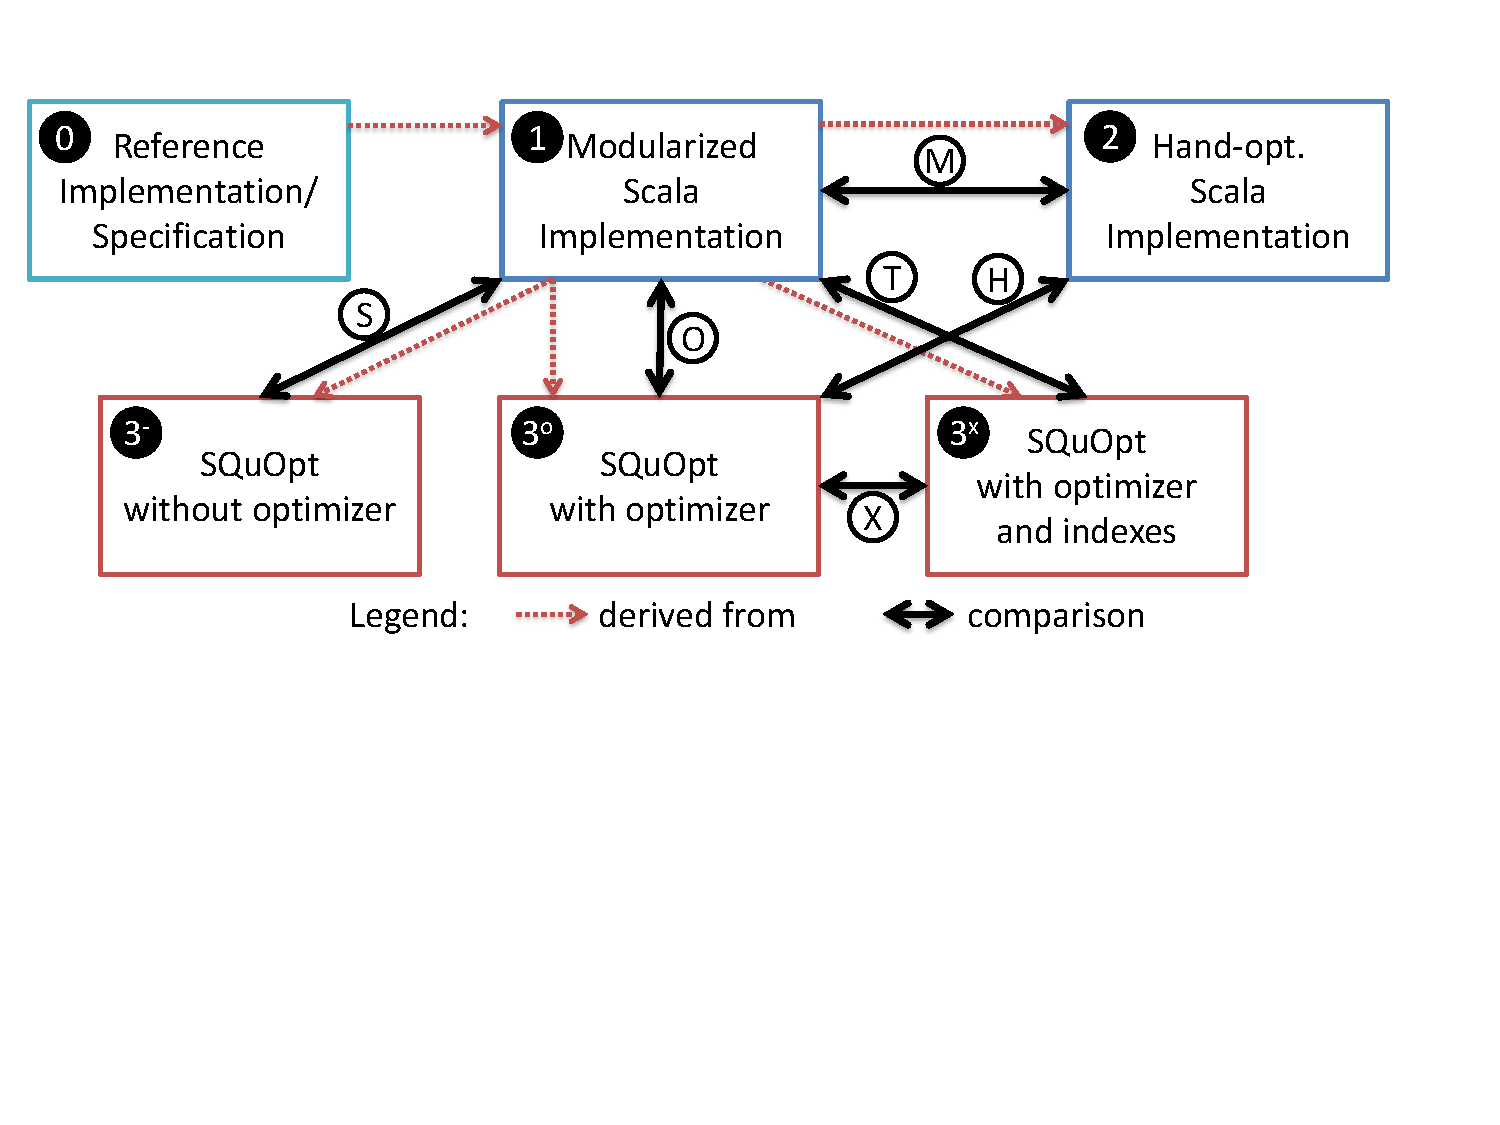
\includegraphics[width=\linewidth]{aosd13/graphs/measurements-overview}
	\caption{Measurement Setup: Overview}
	\label{fig:measurements-overview}
\end{figure}


\section{Experimental Units}




%selecting queries
%\begin{table*}
%\begin{tabular}{ll}\toprule
%Identifier & Description \\ \midrule
%PROTECTED\_FIELD % Findbugs: CI\_CONFUSED\_INHERITANCE
%%	& % Idealized: 4
%	& Class is final but declares protected field \\
%NO\_CLONE % Findbugs: CN\_IDOM
%%	& % Idealized: 9
%	&  Class implements Cloneable but does not define or use clone method \\
%SUPER\_CLONE\_MISSING % Findbugs: CN\_IDIOM\_NO\_SUPER\_CALL
%%	& % Idealized: 11
%	& The clone method does not call super.clone() \\
%NOT\_CLONEABLE % Findbugs: CN\_IMPLEMENTS\_CLONE\_BUT\_NOT\_CLONEABLE
%%	& % Idealized: 5
%	& Class defines clone() but doesn't implement Cloneable\\
%COVARIANT\_COMPARETO % Findbugs CO\_ABSTRACT\_SELF \& CO\_SELF\_NO\_OBJECT
%%	& % Idealized: 7
%	& Covariant compareTo() method defined\\
%GC\_CALL % Findbugs:  DM\_GC
%%	& % Idealized: 12
%	& Explicit garbage collection; extremely dubious except in benchmarking code\\
%RUN\_FINALIZERS\_ON\_EXIT % Findbugs DM\_RUN\_FINALIZERS\_ON\_EXIT
%%	& % Idealized: 12
%	& Method invokes dangerous method runFinalizersOnExit\\
%COVARIANT\_EQUALS %Findbugs: EQ\_ABSTRACT\_SELF
%%	& % Idealized: 4
%	& Abstract class defines covariant equals() method \\
%FINALIZER\_NOT\_PROTECTED % Findbugs: FI_PUBLIC_SHOULD_BE_PROTECTED
%%	& % Idealized: 6
%	& Finalizer should be protected, not public\\
%%NO\_SUITABLE\_CONSTRUCTOR% Findbugs: SE\_NO\_SUITABLE\_CONSTRUCTOR
%%	& % Idealized: 7
%%	& Class is Serializable but its superclass doesn't define a void constructor\\
%UNUSED\_PRIVATE\_FIELD % Findbugs: UUF\_UNUSED\_FIELD
%%	& % Idealized: 23
%	& The value of a private field is not read\\
%DONT\_CATCH\_IMSE  %Findbugs: IMSE\_DONT\_CATCH\_IMSE
%%	& % Idealized: 5
%	& Dubious catching of IllegalMonitorStateException \\\bottomrule
%\end{tabular}
%\nocaptionrule\caption{Implemented Analyses}
%\label{table:implemented-analyses}
%\end{table*}


\newcommand{\captionEvalTable}{%
As in in \cref{sec:implemenationsandspeedups}, (1) denotes the modular Scala
implementation, (2) the hand-optimized Scala one, and ($3^-$), ($3^o$), ($3^x$)
refer to the {\LoS} implementation when run, respectively, without
optimizations, with optimizations, with optimizations and indexing.
Queries marked with the $R$ superscript were selected by random sampling.}
\newcommand{\tablerowsize}{\scriptsize}
\begin{sidewaystable}[ph!]
\centering
\input{\graphPath{EvalTable}}
\nocaptionrule\caption{Performance results. \captionEvalTable}
\label{table:performance}
\end{sidewaystable}



\begin{table}[h]
  \centering
  \footnotesize
\input{\graphPath{EvalSummaryTable}}
\nocaptionrule\caption{Average performance ratios.
This table summarizes all interesting performance ratios across all queries,
using the geometric mean~\citep{Fleming86}.
The meaning of speedups is discussed in \cref{sec:implemenationsandspeedups}.}
\label{table:performanceAvg}
\end{table}

\begin{table}[h!]
\begin{tabular}{p{7cm}r}\toprule
Abstraction & Used \\ \midrule
% calculate class hierarchy & 5 \\
All fields in all class files	& 4\\
All methods in all class files	& 3\\
All method bodies in all class files	& 3\\
All instructions in all method bodies and their bytecode index	& 5\\
Sliding window (size $n$) over all instructions (and their index) &	3\\
\bottomrule
\end{tabular}\\
\nocaptionrule\caption{Description of abstractions removed during hand-optimization and number of queries where the abstraction is used (and optimized away).}
\label{table:implemented-abstractions}
\end{table}

\begin{extraEval}
\begin{table*}[tb]
\centering
\begin{tabular}{l*{3}{r@{}c@{}l}r*{2}{r@{}c@{}l}}\toprule
Name&\multicolumn{3}{c}{Base impl.\ (in ms)}&\multicolumn{3}{c}{Modular impl}&\multicolumn{3}{c}{Optimiz.\ time}&IS&\multicolumn{3}{c}{OS}&\multicolumn{3}{c}{OS-Opt}\\\midrule
\input{\graphPath{table}}
\bottomrule
\end{tabular}
\nocaptionrule\caption{Old performance results table}
\label{table:performanceOld}
\end{table*}
\end{extraEval}


As experimental units, we sampled a set of queries on code structures from FindBugs 2.0~\citep{DBLP:journals/sigplan/HovemeyerP04}. FindBugs is a popular bug-finding tool for Java Bytecode available as open source. To detect instances of bug patterns, it queries a structural in-memory representation of a code base (extracted from bytecode).
Concretely, a single loop traverses each class and invokes all visitors (implemented as listeners) on each element of the class. Many visitors, in turn, perform activities concerning multiple bug detectors which are fused together. An extreme example is that, in FindBugs, query \queryRUNFINALIZERSONEXIT{} is defined in class \code{DumbMethods} together with other 41 bug detectors for distinct types of bugs.
Typically a bug detector is furthermore scattered across the different methods of the visitor, which handle different elements of the class.
We believe this architecture has been chosen to achieve good performance; however, we do not consider such manual fusion of distinct bug detectors together as modular. We selected queries from FindBugs because they represent typical non-trivial queries on in-memory collections and because we believe our framework allows expressing them more modularly.

We sampled queries in two batches. First, we manually selected \manualQueryCount~queries (from approx.\ 400~queries in FindBugs), chosen mainly to evaluate the potential speedups of indexing (queries that primarily looked for declarations of classes, methods, or fields with specific properties, queries that inspect the type hierarchy, and queries that required analyzing methods implementation).
Subsequently, we \emph{randomly} selected a batch of \randomQueryCount~additional queries.
The batch excluded queries that rely on control-/dataflow analyses (i.e., analyzing the effect of bytecode instructions on the stack), due to limitations of the bytecode tookit we use.
In total, we have \queryCount{} queries as listed in \cref{table:performance} (the randomly selected queries are marked with the superscript $R$).




%Omit - this only showcases BAT, not our code. Show our implementation instead.
\begin{figure}[htb]
\centering
%\begin{lstlisting}
%for {
%  cf <- classFiles
%  m @ Method(_, "equals", MethodDescriptor(Seq(cf.thisClass), BooleanType), _) <- cf.methods
%  if m.isAbstract
%} yield (cf, m)
%\end{lstlisting}
%import BATLifting._
\begin{lstlisting}
for {
  classFile <- classFiles.asSquopt
  method <- classFile.methods
  if method.isAbstract && method.name ==# "equals" &&
     method.descriptor.returnType ==# BooleanType
  parameterTypes <- Let(method.descriptor.parameterTypes)
  if parameterTypes.length ==# 1 &&
     parameterTypes(0) ==# classFile.thisClass
} yield (classFile, method)
\end{lstlisting}
\caption{Find covariant \code{equals} methods.}
\label{fig:covariant-equals}
\end{figure}



%reimplementation
We implemented each query three times (see implementations (1)--(3) in \cref{sec:implemenationsandspeedups}) following the specifications given in the FindBugs documentation (0). Instead of using a hierarchy of visitors as the original implementations of the queries in FindBugs, we wrote the queries as for-comprehensions in Scala on an in-memory representation created by the Scala toolkit BAT\@.\footnote{\url{http://github.com/Delors/BAT}}
BAT in particular provides comprehensive support for
writing queries against Java bytecode in an idiomatic way.
We exemplify an analysis in \cref{fig:covariant-equals}: It detects all co-variant \code{equals} methods in a project by iterating over all class files (line 2) and all methods, searching for methods named ``\code{equals}'' that return a boolean value and define a single parameter of the type of the current class.


\smartParagraph{Abstractions}
In the reference implementations (1), we identified several reusable abstractions as shown in \cref{table:implemented-abstractions}.
The reference implementations of all queries except \querySEBADFIELDINNERCLASS{} use exactly one of these abstractions, which encapsulate the main loops of the queries.

\smartParagraph{Indexes}
For executing ($3^x$) (\LoS\ with indexes), we have constructed three indexes to speed up navigation over the queried data of queries 1--\manualQueryCount{}: Indexes for method name, exception handlers, and instruction types. We illustrate the implementation of the method-name index in \cref{fig:indexes}: it produces a collection of all methods and then indexes them using \code{indexBy}; its argument extracts from an entry the key, that is the method name.
We selected which indexes to implement using guidance from \LoS{} itself; during optimizations, \LoS{} reports which indexes it could have applied to the given query. Among those, we tried to select indexes giving a reasonable compromise between construction cost and optimization speedup.
%% If we want to show the raw data, we could use this LaTeX code - but we need updated, and correct, data!
We first measured the construction cost of these indexes:

\begin{center}
\begin{tabular}{l*{1}{r@{}c@{}l}}\toprule
Index&\multicolumn{3}{c}{Elapsed time (ms)}\\\midrule

Method name&$97.99$&$\pm$&$2.94$\\
Exception handlers&$179.29$&$\pm$&$3.21$\\
Instruction type&$4166.49$&$\pm$&$202.85$\\

\bottomrule
\end{tabular}
\end{center}
For our test data, index construction takes less than 200 ms for the first two indexes, which is moderate compared to the time for loading the bytecode in the BAT representation ($\readingClassFilesTime$). Building the instruction index took around 4 seconds, which we consider acceptable since this index maps each type of instruction (e.g.\ \code{INSTANCEOF}) to a collection of all bytecode instructions of that type.
%Valid question: why does the exception-handler index take so much more than the query it optimizes? That's because indexes are interpreted. But it's best not to say it. Also, we already discuss this later convincingly.

%The first index maps any method name to the corresponding methods (together with containing classes), and is used by many different queries. Its implementation is shown in \cref{fig:indexes}: the code shown first produces a collection of all methods and then indexes them using \code{indexBy}; its argument extracts from an entry the key, that is the method name.
%The second index maps any exception type to exception handlers catching them (together with the containing method bodies, methods and class).
%The third index allows to look for occurrences of bytecode instructions of a given type; it maps any type of bytecode instruction (like \code{INVOKESTATIC}, \code{INVOKEVIRTUAL} and so on) to its occurrences.

\begin{figure}
\centering
\begin{lstlisting}
val methodNameIdx: Exp[Map[String, Seq[(ClassFile, Method)]]] = (for {
  classFile <- classFiles.asSquopt
  method <- classFile.methods
} yield (classFile, method)).indexBy(entry => entry._2.name)
\end{lstlisting}
\caption{A simple index definition}
\label{fig:indexes}
\end{figure}



\section{Measurement Setup}
To measure performance, we executed the queries on the preinstalled JDK class library (\texttt{rt.jar}), containing 58M of uncompressed Java bytecode.
We also performed a preliminary evaluation by running queries on the much smaller ScalaTest library, getting comparable results that we hence do not discuss.
Experiments were run on a 8-core Intel Core i7-2600, 3.40 GHz, with 8 GB of RAM, running Scientific Linux release 6.2.
The benchmark code itself is single-threaded, so it uses only one core; however the JVM used also other cores to offload garbage collection.
We used the preinstalled OpenJDK Java version 1.7.0\_05-icedtea and Scala 2.10.0-M7.

We measure steady-state performance as recommended by \citet{Georges07rigorousJavaPerformance}. We invoke the JVM $p = 15$ times;
at the beginning of each JVM invocation, all the bytecode to analyze is loaded in memory and converted into BAT's representation.
In each JVM invocation, we iterate each benchmark until the variations of results becomes low enough. We measure the variations of results through the coefficient of variation (CoV; standard deviation divided by the mean). Thus, we iterate each benchmark until the CoV in the last $k = \kZrememberedSampleLoops$ iterations drops under the threshold $\theta = \thetaZmaxCov$, or until we complete $q = \qZmaxLoops$ iterations.
We report the arithmetic mean of these measurements (and also report the usually low standard deviation on our web page).
%PG: I had p = 3, k = 50, theta = 0.02, q = 1000, but changed the parameters when running more queries.

\section{Results}

\smartParagraph{Correctness} We machine-checked that for each query, all variants in \cref{table:performance} agree.

\smartParagraph{Modularization Overhead}
We first observe that performance suffers significantly when using the abstractions we described in \cref{table:implemented-abstractions}. These abstractions, while natural in the domain and in the setting of a declarative language, are not idiomatic in Java or Scala because, without optimization, they
will obviously lead to bad performance. They are still useful abstractions from the point of view of modularity, though---as indicated by \cref{table:implemented-abstractions}---and as such it would be desirable if one could use them without paying the performance penalty.


\smartParagraph{Scala Implementations vs.\ FindBugs}
Before actually comparing between the different Scala and \LoS\ implementations, we first ensured that the implementations are comparable to the original FindBugs implementation. A direct comparison between the FindBugs reference implementation and any of our implementations is not possible in a rigorous and fair manner. FindBugs bug detectors are not fully modularized, therefore we cannot reasonably isolate the implementation of the selected queries from support code. Furthermore, the architecture of the implementation has many differences that affect performance: among others, FindBugs also uses multithreading. Moreover, while in our case each query loops over all classes, in FindBugs, as discussed above, a single loop considers each class and invokes all visitors (implemented as listeners) on it.

We measured \emph{startup performance}~\citep{Georges07rigorousJavaPerformance}, that is the performance of running the queries only once, to minimize the effect of compiler optimizations.
We setup our \LoS-based analyses to only perform optimization and run the optimized query. To setup FindBugs, we manually disabled all unrelated bug detectors; we also made the modified FindBugs source code available. The result is that the performance of the Scala implementations of the queries ($3^-$) has performance of the same order of magnitude as the original FindBugs queries -- in our tests, the \LoS\ implementation was about twice as fast. However, since the comparison cannot be made fair, we refrained from a more detailed investigation.

% XXX HACK
\smartParagraph{SQuOpt Overhead and Optimization Potential}
We present the results of our benchmarks in \cref{table:performance}.
Column names refer to a few of the definitions described above; for readability, we do not present all the ratios previously introduced for each query, but report the raw data.
In \cref{table:performanceAvg}, we report the geometric mean \cite{Fleming86} of each ratio, computed with the same weight for each query.

%queries are between \maxInterpOver{}x slower and \maxInvInterpOver{}x faster; on average \LoS\ queries are \geoMeanInvInterpOver{}x faster.
%\minInvInterpOver{}x and \maxInvInterpOver{}x---that is, queries are between \minInterpOver{}x and
We see that, in its current implementation, \LoS\ can cause a overhead S
(1/$3^-$) up to \maxInterpOver{}x. On average \LoS\ queries are
\geoMeanInterpOver{}x faster. These differences are due to minor implementation
details of certain collection operators.
For query $18^R$, instead, we have that the the basic \LoS\ implementation is \maxInvInterpOver{}x faster and are investigating the reason; we suspect this might be related to the use of pattern matching in the original query.

As expected, not all queries benefit from optimizations;
out of \queryCount{} queries, optimization affords for \nSpeededUpQueries{} of them significant speedups ranging from a \minOptimSpeedup{} factor to a \maxOptimSpeedup{} factor; \nBigSpeededUpQueries{} queries are faster by a factor of at least \speedupBigThreshold{}.
Only queries \queryMSPKGPROTECT{}, \querySICINNERSHOULDBESTATICANON{} and \queryITAINEFFICIENTTOARRAY{} fail to recover any modularization overhead.

We have analyzed the behavior of a few queries after optimization, to understand why their performance has
(or has not) improved.

Optimization makes query \querySEBADFIELDINNERCLASS{} slower; we believe this is because optimization replaces filtering by lazy filtering, which is usually faster, but not here.
Among queries where indexing succeeds, query \queryGCCALL{} has the least speedup. After optimization, this query uses the instruction-type index to find all occurrences of invocation opcodes (\code{INVOKESTATIC} and \code{INVOKEVIRTUAL}); after this step the query looks, among those invocations, for ones targeting \code{runFinalizersOnExit}. Since invocation opcodes are quite frequent, the used index is not very specific, hence it allows for little speedup (\speedupTGCCALL). However no other index applies to this query; moreover, our framework does not maintain any selectivity statistics on indexes to predict these effects.
Query \queryFIUSELESS{} benefits from indexing without any specific tuning on our part, because it looks for implementations of \code{finalize} with some characteristic, hence the highly selective method-name index applies.
After optimization, query \queryDONTCATCHIMSE{} becomes simply an index lookup on the index for exception handlers, looking for handlers of \code{IllegalMonitorStateException}; it is thus not surprising that its speedup is thus extremely high (\maxOptimSpeedup{}). This speedup relies on an index which is specific for this kind of query, and building this index is slower than executing the unoptimized query. On the other hand, building this index is entirely appropriate in a situation where similar queries are common enough. Similar considerations apply to usage of indexing in general, similarly to what happens in databases.

\smartParagraph{Optimization Overhead}
The current implementation of the optimizer is not yet optimized for speed (of the optimization algorithm). For instance, expression trees are traversed and rebuilt completely once for each transformation.
However, the optimization overhead is usually not excessive and
is $\avgOptimTime \pm \stdDevOptimTime$ ms, varying between \minOptimTime{} ms and \maxOptimTime{} ms (mostly depending on the query size).

\smartParagraph{Limitations}
Although many speedups are encouraging, our optimizer is currently a proof-of-concept and we experienced some limitations:
\begin{itemize}
\item In a few cases hand-optimized queries are still faster than what the optimizer can produce. We believe these problems could be addressed by adding further optimizations.
\item Our implementation of indexing is currently limited to immutable collections. For mutable collections, indexes must be maintained incrementally.
Since indexes are defined as special queries in {\LoS},  incremental index maintenance becomes an instance of incremental maintenance of query results, that is, of incremental view maintenance. We plan to support incremental view maintenance as part of future work; however,
indexing in the current form is already useful, as illustrated by our experimental results.
\end{itemize}

\smartParagraph{Threats to Validity}
With rigorous performance measurements and the chosen setup, our study was setup to maximize internal and construct validity. Although we did not involve an external domain expert and we did not compare the results of our queries with the ones from FindBugs (except while developing the queries), we believe that the queries adequately represent the modularity and performance characteristics of FindBugs and {\LoS}. However, since we selected only queries from a single project, external validity is limited.
While we cannot generalize our results beyond FindBugs yet, we believe that the FindBugs queries are representative for complex in-memory queries performed by applications.


\smartParagraph{Summary}
We demonstrated on our real-world queries that relying on declarative abstractions in collection queries often causes a significant slowdown. As we have seen, using \LoS\ without optimization, or when no optimizations are possible, usually provides performance comparable to using standard Scala; however, \LoS\ optimizations can in most cases remove the slowdown due to declarative abstractions. Furthermore, relying on indexing allows to achieve even greater speedups while still using a declarative programming style.
Some implementation limitations restrict the effectiveness of our optimizer, but since this is a preliminary implementation, we believe our evaluation shows the great potential of optimizing queries to in-memory collections.


% vim: set tw=0:


\section{Related Work}
\label{sec:relwork}
This paper builds on prior work on language-integrated queries, query optimization, techniques for DSL embedding, and other works on code querying.

\smartParagraph{Language-Integrated Queries}
Microsoft's Language-Integrated Query technology (\LINQ)~\citep{Meijer:2006:LRO:1142473.1142552,Bierman:2007:LTF:1297027.1297063} is similar to our work in that it also
reifies queries on collections to enable analysis and optimization. Such queries can be executed against a variety of backends (such as SQL databases or in-memory objects), and adding new back-ends is supported. Its implementation uses \emph{expression trees}, a compiler-supported
implicit conversion between expressions and their reification as a syntax tree. There are various major differences, though.
First, the support for expression trees is hard-coded into the compiler. This means that the techniques are not applicable in languages 
that do not explicitly support expression trees. More importantly, the way expression trees are created in \LINQ\ is generic and fixed.
For instance, it is not possible to create different tree nodes for method calls that are relevant to an analysis (such as the \code{map} method) than for method calls that are irrelevant for the analysis (such as the \code{toString} method). For this reason, expression trees in \LINQ\ 
cannot be customized to the task at hand and contain too much low-level information. It is well-known that this makes it quite hard to
implement programs operating on expression trees~\citep{Eini11Pain}. 

\LINQ\ queries can also not easily be decomposed and modularized. For instance, consider the task of refactoring the filter in the query {\tt from x in y where x.z == 1 select x}
into a function. Defining this function as {\tt bool comp(int v) \{ return v == 1; \}} would destroy the possibility of analyzing the filter for optimization, since
the resulting expression tree would only contain a reference to an opaque function. The function could be declared as returning an expression tree instead, but then
this function could not be used in the original query anymore, since the compiler expects an expression of type {\tt bool} and not an expression tree of type {\tt bool}.
It could only be integrated if the expression tree of the original query is created by hand, without using the built-in support for expression trees.

% Klaus: since we do not talk much about the embedding technique we should not talk about type safety here
%Expression trees in \LINQ\ also provide little type safety. While they appear to be typed superficially (quoting an expression of type \code{T} yields 
%an expression tree of type \code{Expression<T>}) they are untyped internally. For instance, when one decomposes a node into its components,
%the components are untyped. 
% Klaus: let's not distract by talking superficially about Haskell
% This is similar to deep embedding of expressions in Haskell, which typically use a phantom type wrapper around untyped expressions.

%In contrast, expression trees in our approach are typed and simple transformations can be statically checked to be type-preserving. More complex optimizations require however type casts and rely on erasure of type parameters at run time, as we will discuss in detail later on.

Although queries against in-memory collections could theoretically also be optimized in \LINQ, the standard implementation, {\LINQ}2Objects, performs no optimizations. 

A few optimized embedded DSLs allow executing queries or computations on distributed clusters.
DryadLINQ~\citep{Yu08}, based on \LINQ, optimizes queries for distributed
execution. It inherits \LINQ's limitations and thus does not support decomposing queries in different modules.
Modularizing queries is supported instead by FlumeJava~\citep{Chambers10},
another library (in Java) for distributed query execution.
However, FlumeJava cannot express many optimizations because its representation
of expressions is more
limited; also, its query language is more cumbersome. Both problems are rooted
in Java's limited support for embedded DSLs.
Other embedded DSLs support parallel platforms such as GPUs or many-core CPUs,
such as Delite~\citep{Rompf13}.

\citet{Willis06JQL,Willis08} add first-class queries to Java through a source-to-source translator and implement a few selected optimizations, including join order optimization and incremental maintenance of query results.
They investigate how well their techniques apply to Java programs, and they suggest that programmers use manual optimizations to avoid expensive constructs like nested loops. While the goal of these works is similar to ours, their implementation as an external source-to-source-translator makes
the adoption, extensibility, and composability of their technique difficult%
%~\citep{ErdwegGR12}
.
%KO: not sure whether the reference here helps
%PG: Remove it if we have space limits.

There have been many approaches for a closer integration of SQL queries into programs, such as
HaskellDB~\citep{Leijen99DSEC} (which also inspired \LINQ), or Ferry~\citep{Grust:2009:FDP:1559845.1559982} 
(which moves part of a program execution to a database). In Scala, there are also
APIs which integrate SQL queries more closely such as
Slick.\footnote{\url{http://slick.typesafe.com/}} Its frontend allows to define
and combine type-safe queries, similarly to ours (also in the way it is
implemented).
However, the language for defining queries maps to SQL, so it does not support nesting collections
in other collections (a feature which simplified our example in
Sec.~\ref{sec:motivation}), nor distinguishes statically between different kinds of
collections, such as \code{Set} or \code{Seq}.
Based on Ferry, ScalaQL~\citep{JOT:issue_2010_07/article3} extends Scala with a compiler-plugin to integrate a query language on top of a relational database. The work by \citet{Spiewak09scalaql:language-integrated} is
 unrelated to~\citep{JOT:issue_2010_07/article3} but also called ScalaQL\@. It is similar to our approach in that it also 
proposes to reify queries based on for-comprehensions, but it is not clear from the paper how the reification 
works.\footnote{We contacted the authors; they were not willing to provide more details or the sources of their approach.}


\smartParagraph{Query Optimization}
Query optimization on relational data is a long-standing issue in the database community, but there
are also many works on query optimization on objects~\citep{Fegaras00,Grust99PhD}.
Compared to these works, we have only implemented a few simple query optimizations, so there is potential
for further improvement of our work by incorporating more advanced optimizations.

%CQEngine (\url{http://code.google.com/p/cqengine/}) does not support path
%indexes. It support standing queries - but those are just incrementally
%maintained queries, as far as it seems. But the system is quite cool.
%---

% That's not strictly true, and is not the point. The point is a consequence: in a monoid comprehension for a given monoid, a generator cannot range over a monoid which is weaker wrt.\ idempotence or commutativity.

%For instance, while the formal analogous of folds in their calculus is a monoid homomorphism, computing the size of a Set can be expressed through a fold but not through a monoid homomorphism, since it is a fold from an idempotent to a non-idempotent monoid.

% Klaus: I think this is not that relevant for ICSE
%\citet{Henglein10} present an embedding of the relational algebra in Haskell.
%Queries are not reified in their approach, but due to a particularly sophisticated
%representation of multisets it is possible to execute some queries containing
%cross-products using faster equi-joins.


\smartParagraph{Scala and DSL Embedding}
\label{sec:rwdsl}
Technically, our implementation of \LoS\ is a deep embedding of a part of the Scala collections API~\citep{odersky2009fighting}.
Deep embeddings were pionereed by \citet{Leijen99DSEC} and \citet{elliott03compiling}. The technical
details of the embedding are not the main topic of this paper; we are using some of the 
Scala techniques presented by \citet{rompf2010lightweight} for using implicits and for
adding infix operators to a type. Similar to \citet{rompf2010lightweight}, we also 
use the Scala compiler on-the-fly. A plausible alternative backend for \LoS\ would
have been to use Delite~\citep{Rompf11BBlocks}, a framework for
building highly efficient DSLs in Scala.
Using this framework, in concurrent work, \citet{Rompf13} also optimize
collection queries; while their work allows for imperative programs, they do
not support embedding arbitrary libraries in an automated way. On the other
hand, they can reuse support for automatic parallelization and multiple platforms present in Delite.
\citet{Ackermann12} present Jet, which also optimizes collection queries but
targets MapReduce-style computations in a distributed environment.
Moreover, both works do not apply typical database optimizations such as
indexing or filter hoisting.


We regard the Scala collections API~\citep{odersky2009fighting} as a shallowly embedded query DSL\@. Query operators immediately perform collection operations when called, so that it is not possible to optimize queries before execution. In addition to these eager query operators, the Scala collections API also provides \emph{views} to create lazy collections.
Views are somewhat similar to {\LoS} in that they reify query operators as data structures and interpret them later.
However, views are not used for automatic query optimization, but for explicitly changing the evaluation order of collection processing. Unfortunately, views are not suited as a basis for the implementation of {\LoS} because they only reify the outermost pipeline of collection operators, whereas nested collection operators as well as other Scala code in queries, such as filter predicates or \code{map} and \code{flatMap} arguments, are only shallowly embedded.
Deep embedding of the whole query is necessary for many optimizations, as discussed in Sec.~\ref{sec:solution}.

\smartParagraph{Code Querying}
In our evaluation we explore the usage of \LoS\ to express queries on code and re-implement a subset of the FindBugs~\citep{DBLP:journals/sigplan/HovemeyerP04} analyses. There are various other specialized code query languages such as 
CodeQuest~\citep{Hajiyev06CodeQuest} or D-CUBED~\citep{Wegrzynowicz:2009:GBU:1639950.1640032}. 
Since these are special-purpose query languages that are not embedded into a host language, they are not directly comparable to our approach.



\section{Future Work}
As part of future work we plan to add support for \emph{incremental view
maintenance}~\citep{GlucheGrust97Incr} to \LoS. This would allow, for instance,
to update incrementally both indexes and query results.

To make our DSL more convenient to use, it would be useful to use the
virtualized pattern matcher of Scala 2.10, when it will be more robust, to add
support for pattern matching in our virtualized queries.

Finally, while our optimizations are type-safe, as they rewrite an expression
tree to another of the same type, currently the Scala
type-checker cannot verify this statically, because of its limited support for
GADTs.
Solving this problem conveniently would allow checking statically that
transformations are safe and make developing them easier.

\section{Conclusions}

We have illustrated the tradeoff between performance and modularity for queries on in-memory collections. We have shown that it is possible to design a deep embedding of a version of the collections API which reifies queries and can optimize them at runtime.
Writing queries using this framework is, except minor syntactic details, the same as writing queries using the collection library, hence the adoption barrier to using our optimizer is low. 

Our evaluation shows that using abstractions in queries introduces a significant
performance overhead with native Scala code, while \LoS{}, in most cases, makes
the overhead much more tolerable or removes it completely. Optimizations are not
sufficient on some queries, but since our optimizer is a proof-of-concept with
many opportunities for improvement, we believe a more elaborate version will
achieve even better performance and reduce these limitations.


%\section*{Acknowledgements}
\smartParagraph{Acknowledgements}
The authors thank Sebastian Erdweg for helpful discussions on
this project, Katharina Haselhorst for help
implementing the code generator, and the anonymous reviewers, Jacques Carette and Karl Klose
for their helpful comments on this paper.
This work is supported in part by the European Research Council, grant \#203099 ``ScalPL''.



\part{Incrementalization by static differentiation}
\label{part:incr}
% Emacs, this is -*- latex -*-!
%% ODER: format ==         = "\mathrel{==}"
%% ODER: format /=         = "\neq "
%
%
\makeatletter
\@ifundefined{lhs2tex.lhs2tex.sty.read}%
  {\@namedef{lhs2tex.lhs2tex.sty.read}{}%
   \newcommand\SkipToFmtEnd{}%
   \newcommand\EndFmtInput{}%
   \long\def\SkipToFmtEnd#1\EndFmtInput{}%
  }\SkipToFmtEnd

\newcommand\ReadOnlyOnce[1]{\@ifundefined{#1}{\@namedef{#1}{}}\SkipToFmtEnd}
\usepackage{amstext}
\usepackage{amssymb}
\usepackage{stmaryrd}
\DeclareFontFamily{OT1}{cmtex}{}
\DeclareFontShape{OT1}{cmtex}{m}{n}
  {<5><6><7><8>cmtex8
   <9>cmtex9
   <10><10.95><12><14.4><17.28><20.74><24.88>cmtex10}{}
\DeclareFontShape{OT1}{cmtex}{m}{it}
  {<-> ssub * cmtt/m/it}{}
\newcommand{\texfamily}{\fontfamily{cmtex}\selectfont}
\DeclareFontShape{OT1}{cmtt}{bx}{n}
  {<5><6><7><8>cmtt8
   <9>cmbtt9
   <10><10.95><12><14.4><17.28><20.74><24.88>cmbtt10}{}
\DeclareFontShape{OT1}{cmtex}{bx}{n}
  {<-> ssub * cmtt/bx/n}{}
\newcommand{\tex}[1]{\text{\texfamily#1}}	% NEU

\newcommand{\Sp}{\hskip.33334em\relax}


\newcommand{\Conid}[1]{\mathit{#1}}
\newcommand{\Varid}[1]{\mathit{#1}}
\newcommand{\anonymous}{\kern0.06em \vbox{\hrule\@width.5em}}
\newcommand{\plus}{\mathbin{+\!\!\!+}}
\newcommand{\bind}{\mathbin{>\!\!\!>\mkern-6.7mu=}}
\newcommand{\rbind}{\mathbin{=\mkern-6.7mu<\!\!\!<}}% suggested by Neil Mitchell
\newcommand{\sequ}{\mathbin{>\!\!\!>}}
\renewcommand{\leq}{\leqslant}
\renewcommand{\geq}{\geqslant}
\usepackage{polytable}

%mathindent has to be defined
\@ifundefined{mathindent}%
  {\newdimen\mathindent\mathindent\leftmargini}%
  {}%

\def\resethooks{%
  \global\let\SaveRestoreHook\empty
  \global\let\ColumnHook\empty}
\newcommand*{\savecolumns}[1][default]%
  {\g@addto@macro\SaveRestoreHook{\savecolumns[#1]}}
\newcommand*{\restorecolumns}[1][default]%
  {\g@addto@macro\SaveRestoreHook{\restorecolumns[#1]}}
\newcommand*{\aligncolumn}[2]%
  {\g@addto@macro\ColumnHook{\column{#1}{#2}}}

\resethooks

\newcommand{\onelinecommentchars}{\quad-{}- }
\newcommand{\commentbeginchars}{\enskip\{-}
\newcommand{\commentendchars}{-\}\enskip}

\newcommand{\visiblecomments}{%
  \let\onelinecomment=\onelinecommentchars
  \let\commentbegin=\commentbeginchars
  \let\commentend=\commentendchars}

\newcommand{\invisiblecomments}{%
  \let\onelinecomment=\empty
  \let\commentbegin=\empty
  \let\commentend=\empty}

\visiblecomments

\newlength{\blanklineskip}
\setlength{\blanklineskip}{0.66084ex}

\newcommand{\hsindent}[1]{\quad}% default is fixed indentation
\let\hspre\empty
\let\hspost\empty
\newcommand{\NB}{\textbf{NB}}
\newcommand{\Todo}[1]{$\langle$\textbf{To do:}~#1$\rangle$}

\EndFmtInput
\makeatother
%
%
%
%
%
%
% This package provides two environments suitable to take the place
% of hscode, called "plainhscode" and "arrayhscode". 
%
% The plain environment surrounds each code block by vertical space,
% and it uses \abovedisplayskip and \belowdisplayskip to get spacing
% similar to formulas. Note that if these dimensions are changed,
% the spacing around displayed math formulas changes as well.
% All code is indented using \leftskip.
%
% Changed 19.08.2004 to reflect changes in colorcode. Should work with
% CodeGroup.sty.
%
\ReadOnlyOnce{polycode.fmt}%
\makeatletter

\newcommand{\hsnewpar}[1]%
  {{\parskip=0pt\parindent=0pt\par\vskip #1\noindent}}

% can be used, for instance, to redefine the code size, by setting the
% command to \small or something alike
\newcommand{\hscodestyle}{}

% The command \sethscode can be used to switch the code formatting
% behaviour by mapping the hscode environment in the subst directive
% to a new LaTeX environment.

\newcommand{\sethscode}[1]%
  {\expandafter\let\expandafter\hscode\csname #1\endcsname
   \expandafter\let\expandafter\endhscode\csname end#1\endcsname}

% "compatibility" mode restores the non-polycode.fmt layout.

\newenvironment{compathscode}%
  {\par\noindent
   \advance\leftskip\mathindent
   \hscodestyle
   \let\\=\@normalcr
   \let\hspre\(\let\hspost\)%
   \pboxed}%
  {\endpboxed\)%
   \par\noindent
   \ignorespacesafterend}

\newcommand{\compaths}{\sethscode{compathscode}}

% "plain" mode is the proposed default.
% It should now work with \centering.
% This required some changes. The old version
% is still available for reference as oldplainhscode.

\newenvironment{plainhscode}%
  {\hsnewpar\abovedisplayskip
   \advance\leftskip\mathindent
   \hscodestyle
   \let\hspre\(\let\hspost\)%
   \pboxed}%
  {\endpboxed%
   \hsnewpar\belowdisplayskip
   \ignorespacesafterend}

\newenvironment{oldplainhscode}%
  {\hsnewpar\abovedisplayskip
   \advance\leftskip\mathindent
   \hscodestyle
   \let\\=\@normalcr
   \(\pboxed}%
  {\endpboxed\)%
   \hsnewpar\belowdisplayskip
   \ignorespacesafterend}

% Here, we make plainhscode the default environment.

\newcommand{\plainhs}{\sethscode{plainhscode}}
\newcommand{\oldplainhs}{\sethscode{oldplainhscode}}
\plainhs

% The arrayhscode is like plain, but makes use of polytable's
% parray environment which disallows page breaks in code blocks.

\newenvironment{arrayhscode}%
  {\hsnewpar\abovedisplayskip
   \advance\leftskip\mathindent
   \hscodestyle
   \let\\=\@normalcr
   \(\parray}%
  {\endparray\)%
   \hsnewpar\belowdisplayskip
   \ignorespacesafterend}

\newcommand{\arrayhs}{\sethscode{arrayhscode}}

% The mathhscode environment also makes use of polytable's parray 
% environment. It is supposed to be used only inside math mode 
% (I used it to typeset the type rules in my thesis).

\newenvironment{mathhscode}%
  {\parray}{\endparray}

\newcommand{\mathhs}{\sethscode{mathhscode}}

% texths is similar to mathhs, but works in text mode.

\newenvironment{texthscode}%
  {\(\parray}{\endparray\)}

\newcommand{\texths}{\sethscode{texthscode}}

% The framed environment places code in a framed box.

\def\codeframewidth{\arrayrulewidth}
\RequirePackage{calc}

\newenvironment{framedhscode}%
  {\parskip=\abovedisplayskip\par\noindent
   \hscodestyle
   \arrayrulewidth=\codeframewidth
   \tabular{@{}|p{\linewidth-2\arraycolsep-2\arrayrulewidth-2pt}|@{}}%
   \hline\framedhslinecorrect\\{-1.5ex}%
   \let\endoflinesave=\\
   \let\\=\@normalcr
   \(\pboxed}%
  {\endpboxed\)%
   \framedhslinecorrect\endoflinesave{.5ex}\hline
   \endtabular
   \parskip=\belowdisplayskip\par\noindent
   \ignorespacesafterend}

\newcommand{\framedhslinecorrect}[2]%
  {#1[#2]}

\newcommand{\framedhs}{\sethscode{framedhscode}}

% The inlinehscode environment is an experimental environment
% that can be used to typeset displayed code inline.

\newenvironment{inlinehscode}%
  {\(\def\column##1##2{}%
   \let\>\undefined\let\<\undefined\let\\\undefined
   \newcommand\>[1][]{}\newcommand\<[1][]{}\newcommand\\[1][]{}%
   \def\fromto##1##2##3{##3}%
   \def\nextline{}}{\) }%

\newcommand{\inlinehs}{\sethscode{inlinehscode}}

% The joincode environment is a separate environment that
% can be used to surround and thereby connect multiple code
% blocks.

\newenvironment{joincode}%
  {\let\orighscode=\hscode
   \let\origendhscode=\endhscode
   \def\endhscode{\def\hscode{\endgroup\def\@currenvir{hscode}\\}\begingroup}
   %\let\SaveRestoreHook=\empty
   %\let\ColumnHook=\empty
   %\let\resethooks=\empty
   \orighscode\def\hscode{\endgroup\def\@currenvir{hscode}}}%
  {\origendhscode
   \global\let\hscode=\orighscode
   \global\let\endhscode=\origendhscode}%

\makeatother
\EndFmtInput
%
%
%
% First, let's redefine the forall, and the dot.
%
%
% This is made in such a way that after a forall, the next
% dot will be printed as a period, otherwise the formatting
% of `comp_` is used. By redefining `comp_`, as suitable
% composition operator can be chosen. Similarly, period_
% is used for the period.
%
\ReadOnlyOnce{forall.fmt}%
\makeatletter

% The HaskellResetHook is a list to which things can
% be added that reset the Haskell state to the beginning.
% This is to recover from states where the hacked intelligence
% is not sufficient.

\let\HaskellResetHook\empty
\newcommand*{\AtHaskellReset}[1]{%
  \g@addto@macro\HaskellResetHook{#1}}
\newcommand*{\HaskellReset}{\HaskellResetHook}

\global\let\hsforallread\empty

\newcommand\hsforall{\global\let\hsdot=\hsperiodonce}
\newcommand*\hsperiodonce[2]{#2\global\let\hsdot=\hscompose}
\newcommand*\hscompose[2]{#1}

\AtHaskellReset{\global\let\hsdot=\hscompose}

% In the beginning, we should reset Haskell once.
\HaskellReset

\makeatother
\EndFmtInput


% https://github.com/conal/talk-2015-essence-and-origins-of-frp/blob/master/mine.fmt
% Complexity notation:






% If an argument to a formatting directive starts with let, lhs2TeX likes to
% helpfully prepend a space to the let, even though that's seldom desirable.
% Write lett to prevent that.













































% Hook into forall.fmt:
% Add proper spacing after forall-generated dots.











% We shouldn't use /=, that means not equal (even if it can be overriden)!







% XXX



%  format `stoup` = "\blackdiamond"






% Cancel the effect of \; (that is \thickspace)



% Use as in |vapply vf va (downto n) v|.
% (downto n) is parsed as an application argument, so we must undo the produced
% spacing.

% indexed big-step eval
% without environments
% big-step eval
% change big-step eval








% \, is 3mu, \! is -3mu, so this is almost \!\!.


\def\deriveDefCore{%
\begin{align*}
  \ensuremath{\Derive{\lambda (\Varid{x}\typcolon\sigma)\to \Varid{t}}} &= \ensuremath{\lambda (\Varid{x}\typcolon\sigma)\;(\Varid{dx}\typcolon\Delta \sigma)\to \Derive{\Varid{t}}} \\
  \ensuremath{\Derive{\Varid{s}\;\Varid{t}}} &= \ensuremath{\Derive{\Varid{s}}\;\Varid{t}\;\Derive{\Varid{t}}} \\
  \ensuremath{\Derive{\Varid{x}}} &= \ensuremath{\Varid{dx}} \\
  \ensuremath{\Derive{\Varid{c}}} &= \ensuremath{\DeriveConst{\Varid{c}}}
\end{align*}
}


% Drop unsightly numbers from function names. The ones at the end could be
% formatted as subscripts, but not the ones in the middle.


\part*{Appendixes}
\addcontentsline{toc}{part}{Appendixes}

\chapter[Preliminaries]{Preliminaries: syntax and semantics of
  simply-typed λ-calculus}
\label{sec:preliminaries}

To discuss how we incrementalize programs and prove that
our incrementalization technique gives correct results, we specify
which foundation we use for our proofs and what object language we
study throughout most of \cref{part:incr}.

We mechanize our correctness proof using Agda, hence we use
Agda's underlying type theory as our foundation. We discuss
what this means in \cref{sec:metalanguage}.

Our object language is a standard simply-typed $\lambda$-calculus
(STLC)~\citep[Ch.~9]{Pierce02TAPL}, parameterized over base types
and constants. We term the set of base types and constants a
\emph{language plugin} (see \cref{sec:lang-plugins}). In our
examples we assume that the language plugins supports needed base
types and constants. Later (e.g., in \cref{ch:derive-formally})
we add further requirements to language plugins, to support
incrementalization of the language features they add to our STLC\@.
%
Rather than operational semantics we use a denotational
semantics, which is however set-theoretic rather than
domain-theoretic. Our object language and its semantics are
summarized in \cref{fig:lambda-calc}.

At this point, readers might want to skip to \cref{sec:intro}
right away, or focus on denotational semantics, and refer to this
section as needed.

\section{Our proof meta-language}
\label{sec:metalanguage}
In this section we describe the logic (or meta-language) used in our
\emph{mechanized} correctness proof.

First, as usual, we distinguish between ``formalization'' (that
is, on-paper formalized proofs) and ``mechanization'' (that is,
proofs encoded in the language of a proof assistant for
computer-aided \emph{mechanized} verification).

To prove the correctness of \ILC, we provide a mechanized proof
in Agda~\citep{agda-head}. Agda implements intensional Martin-Löf
type theory (from now on, simply type theory), so type theory is
also the foundation of our proofs.

At times, we use conventional set-theoretic language to discuss
our proofs, but the differences are only superficial. For
instance, we might talk about a set of elements \ensuremath{\Conid{S}} and with
elements such as \ensuremath{\Varid{s}\in \Conid{S}}, though we always mean that \ensuremath{\Conid{S}} is
a metalanguage type, that \ensuremath{\Varid{s}} is a metalanguage value, and that \ensuremath{\Varid{s}\typcolon\Conid{S}}.
Talking about sets
avoids ambiguity between types of our meta-language and types of
our object-language (that we discuss next in
\cref{sec:intro-stlc}).
\begin{notation}
  We'll let uppercase latin letters \ensuremath{\Conid{A},\Conid{B},\Conid{C}\ldots,\Conid{V},\Conid{U}} range
  over sets, never over types.
\end{notation}

We do not prove correctness of all our language plugins. However,
in earlier work~\citep{CaiEtAl2014ILC} we prove correctness for
a language plugin supporting \emph{bags}, a type of collection (described in
\cref{sec:motiv-example}). For that proof, we extend our logic by
postulating a few standard axioms on the implementation of bags,
to avoid proving correct an implementation of bags, or needing to
account for different values representing the same bag (such
different values typically arise when implementing bags as search
trees).

\subsection{Type theory versus set theory}
Here we summarize a few features of type theory over set theory.

Type theory is dependently typed, so it generalizes
function type \ensuremath{\Conid{A}\to \Conid{B}} to \emph{dependent} function type \ensuremath{(\Varid{x}\typcolon\Conid{A})\to \Conid{B}}, where \ensuremath{\Varid{x}} can appear free in \ensuremath{\Conid{B}}. Such a type guarantees
that if we apply a function \ensuremath{\Varid{f}\typcolon(\Varid{x}\typcolon\Conid{A})\to \Conid{B}} to an argument \ensuremath{\Varid{a}\typcolon\Conid{A}}, the result has type \ensuremath{\Conid{B}\;[\mskip1.5mu \Varid{x}\mathbin{:=}\Varid{a}\mskip1.5mu]}, that is \ensuremath{\Conid{B}} where \ensuremath{\Varid{x}}
is substituted by \ensuremath{\Varid{a}}. At times, we will use dependent types in
our presentation.

Moreover, by using type theory:
\begin{itemize}
\item We do not postulate the law of excluded middle; that is,
  our logic is constructive.
\item Unlike set theory, type theory is proof-relevant: that is,
  proofs are first-class mathematical objects.
\item Instead of subsets
  $\{x \in A \mid P(x)\}$, we must use $\Sigma$-types
  $\Sigma (x : A) P(x)$ which contain pairs of elements $x$ and
  proofs they satisfy predicate $P$.
\item In set theory, we can assume without further ado functional
  extensionality, that is, that functions that give equal results
  on all equal inputs are equal themselves. Intuitionistic type
  theory does not prove functional extensionality, so we need to
  add it as a postulate. In Agda, this postulate is known to be
  consistent~\citep{Hofmann96}, hence it is safe to assume%
  \footnote{\url{http://permalink.gmane.org/gmane.comp.lang.agda/2343}}.
%\item All our function spaces are limited to computable functions.
\end{itemize}

To handle binding issues in our object language, our
formalization uses typed de Bruijn indexes, because this
techniques takes advantage of Agda's support for type refinement
in pattern matching. On top of that, we implement a HOAS-like
frontend, which we use for writing specific terms.

% Our Agda formalization, Scala implementation and benchmark
% results are available at the URL
% \url{http://inc-lc.github.io/}.
% All lemmas and theorems presented
% in this chapter have been proven in Agda.
% In the chapter, we present an overview of
% the formalization in more human-readable form, glossing over some
% technical details.

\section{Simply-typed λ-calculus}
\label{sec:intro-stlc}

We consider as object language a strongly-normalizing
simply-typed $\Gl$-calculus (STLC). We choose STLC as it is the
simplest language with first-class functions and types, while
being a sufficient model of realistic total languages.%
\footnote{To know why we restrict to total languages see
  \cref{sec:general-recursion}.}
%
We recall the syntax and typing rules of STLC in
\cref{fig:lambda-calc:syntax,fig:lambda-calc:typing}, together
with metavariables we use. Language plugins define base types
\ensuremath{\iota} and constants \ensuremath{\Varid{c}}. Types can be base types \ensuremath{\iota} or
function types \ensuremath{\sigma\to \tau}. Terms can be constants \ensuremath{\Varid{c}},
variables \ensuremath{\Varid{x}}, function applications \ensuremath{\Varid{t}_{1}\;\Varid{t}_{2}} or
$\lambda$-abstractions \ensuremath{\lambda (\Varid{x}\typcolon\sigma)\to \Varid{t}}. To describe
assumptions on variable types when typing terms, we define (typing)
contexts \ensuremath{\Gamma} as being either empty \ensuremath{\EmptyContext}, or as context
extensions \ensuremath{\Gamma,\Varid{x}\typcolon\tau}, which extend context \ensuremath{\Gamma} by
asserting variable \ensuremath{\Varid{x}} has type \ensuremath{\tau}. Typing is defined through
a judgment \ensuremath{\Gamma\vdash\Varid{t}\typcolon\tau}, stating that term \ensuremath{\Varid{t}} under
context \ensuremath{\Gamma} has type \ensuremath{\tau}.%
%
\footnote{We only formalize typed terms, not untyped ones, so
  that each term has a unique type. That is, in the relevant
  jargon, we use \emph{Church-style} typing as opposed to
  \emph{Curry-style} typing.
  Alternatively, we use an
  intrinsically-typed term representation.
  In fact, arguably we mechanize at
  once both well-typed terms and their typing derivations. This
  is even more clear in our mechanization; see discussion
  in~\cref{sec:sem-style-and-rw}.}
%
For a proper introduction to STLC we refer the reader to
\citet[Ch.~9]{Pierce02TAPL}. We will assume significant
familiarity with it.

\begin{figure*}
    \small
    \centering

  \NewDocumentCommand{\Align}{m}
    {{\begin{align*}#1\end{align*}}}

    \begin{subfigure}[b]{0.6\textwidth}
\begin{tabular}{>{$}r<{$}@{$\;::=\;$}>{$}c<{$}@{$\;$}>{$}l<{$}@{\quad}>{(}l<{)}}
\Gi      & \rlap{\ldots} &                       & base types\\
\Gs, \Gt & \Gi           & \mid \Fun{\Gt}{\Gt}   & types\\
\GG      & \EmptyContext & \mid \Extend{x}{\tau} & typing contexts\\
c        & \rlap{\ldots} &                       & constants\\
s, t     & c             & \mid \Lam{x}{t}
                           \mid \App{t}{t}
                           \mid x                & terms
\end{tabular}
    \Subcaption{fig:lambda-calc:syntax}
      {Syntax}
%\label{fig:syntax}
    \end{subfigure}
%
    \vfill
%
    \begin{subfigure}[b]{\textwidth}
    \begin{typing}
\noindent
\Rule[Const]
  {\ldots}
  {\Typing[]{c}{\tau}}

\Axiom[Lookup]
  {\Typing[\Append{\GG_1}{\Append{\HasType{x}{\tau}}{\GG_2}}]{\Var{x}}{\tau}}

\raisebox{0.5\baselineskip}{\fbox{$\Typing{t}{\tau}$}}

\Rule[Lam]
  {\Typing[\Extend{x}{\Gs}]{t}{\Gt}}
  {\Typing{\Lam{x}{t}}{\Fun{\Gs}{\Gt}}}

\Rule[App]
  {\Typing{s}{\Fun{\Gs}{\Gt}}\\
   \Typing{t}{\Gs}}
  {\Typing{\App{s}{t}}{\Gt}}
\end{typing}
    \Subcaption{fig:lambda-calc:typing}
      {Typing}
%\label{fig:typing}
    \end{subfigure}
    \vfill

    \begin{subfigure}[b]{0.3\textwidth}
    \Align{
      \Eval{\iota}
        & = \ldots\\
      \Eval{\Fun{\Gs}{\Gt}}
        & = \Eval{\Gs} \to \Eval{\Gt}
    }
    \Subcaption{fig:lambda-calc:values}{
      Values.
    }
  \end{subfigure}
  \hfill
    \begin{subfigure}[b]{0.6\textwidth}
    \Align{
      \Eval{\EmptyContext}
        & = \left\{ \EmptyEnv \right\} \\
      \Eval{\Extend{x}{\Gt}}
        & = \left\{ \ExtendEnv*{x}{v} \mid \Gr \in \Eval{\GG} \land v \in \Eval{\Gt}\right\}
    }
    \Subcaption{fig:lambda-calc:environments}{
      Environments.
    }
  \end{subfigure}
  \begin{subfigure}[b]{0.5\textwidth}
    \Align{
      \EvalWith{c}{\rho}
        & =\EvalConst{c}\\
      \EvalWith{\Lam{x}{t}}{\rho}
        & = \lambda v.\ \EvalWith{t}{\ExtendEnv*{x}{v}}\\
      \EvalWith{\App{s}{t}}{\rho}
        & = \App{\EvalWith*{s}{\rho}}{\EvalWith*{t}{\rho}}\\
      \EvalWith{x}{\Gr}
        & = \textit{lookup $x$ in $\Gr$}
    }
    \Subcaption{fig:lambda-calc:evaluation}{
      Denotational semantics.
    }
  \end{subfigure}
  \caption{Standard definitions for the simply-typed lambda calculus.}
    \label{fig:lambda-calc}
\end{figure*}


\paragraph{An extensible syntax of types}
In fact, the definition of base types can be mutually recursive
with the definition of types. So a language plugin might add as
base types, for instance, collections of elements of type \ensuremath{\tau},
products and sums of type \ensuremath{\sigma} and type \ensuremath{\tau}, and so on.
%
However, this mutual recursion must satisfy a few technical
restrictions to avoid introducing subtle inconsistencies, and
Agda cannot enforce these restrictions across modules. Hence, if
we define language plugins as separate modules in our
mechanization, we need to verify \emph{by hand} that such
restrictions are satisfied (which they are). See
\cref{sec:modularity-limits} for the gory details.

\begin{notation}
We typically omit type annotations on $\lambda$-abstractions,
that is we write \ensuremath{\lambda \Varid{x}\to \Varid{t}} rather than \ensuremath{\lambda (\Varid{x}\typcolon\sigma)\to \Varid{t}}. Such
type annotations can often be inferred from context (or type
inference). Nevertheless, whenever we discuss terms of shape \ensuremath{\lambda \Varid{x}\to \Varid{t}}, we're in fact discussing \ensuremath{\lambda (\Varid{x}\typcolon\sigma)\to \Varid{t}} for some
arbitrary \ensuremath{\sigma}. We write \ensuremath{\lambda \Varid{x}\to \Varid{t}} instead of %
$\Gl x .\ t$, %
for consistency with the notation we use later for Haskell
programs.

We often omit \ensuremath{\EmptyContext} from typing contexts with some assumptions.
For instance we write \ensuremath{\Varid{x}\typcolon\tau_{1},\Varid{y}\typcolon\tau_{2}} instead of \ensuremath{\EmptyContext,\Varid{x}\typcolon\tau_{1},\Varid{y}\typcolon\tau_{2}}.

We overload symbols (often without warning) when they can be
disambiguated from context, especially when we can teach modern
programming languages to disambiguate such overloadings. For
instance, we reuse \ensuremath{\to } for lambda abstractions \ensuremath{\lambda \Varid{x}\to \Varid{t}},
function spaces \ensuremath{\Conid{A}\to \Conid{B}}, and function types \ensuremath{\sigma\to \tau}, even
though the first is the separator.
\end{notation}

\paragraph{Extensions}
In our examples, we will use some unproblematic syntactic sugar
over STLC, including let expressions, global definitions, type
inference, and we will use a Haskell-like concrete syntax. In
particular, when giving type signatures or type annotations in
Haskell snippets, we will use \ensuremath{\mathrel{:\mkern-1mu:}} to separate terms or variables
from their types, rather than \ensuremath{\typcolon} as in
$\lambda$-calculus. To avoid confusion, we never use \ensuremath{\typcolon} to
denote the constructor for Haskell lists.

At times, our concrete examples will use Hindley-Milner (prenex)
polymorphism, but this is also not such a significant extension.
A top-level definition using prenex polymorphism, that is of type
\ensuremath{\forall \alpha\hsforall \hsdot{\circ }{\mathpunct{.}}\tau} (where \ensuremath{\alpha} is free in \ensuremath{\tau}), can be
taken as sugar for a metalevel family of object-level programs,
indexed by type argument \ensuremath{\tau_{1}} of definitions of type \ensuremath{\tau\;[\mskip1.5mu \alpha\mathbin{:=}\tau_{1}\mskip1.5mu]}. We use this trick without explicit mention in
our first implementation of incrementalization in
Scala~\citep{CaiEtAl2014ILC}.

\subsection{Denotational semantics for STLC}
\label{sec:denotational-sem}
To prove that incrementalization preserves the semantics of our
object-language programs, we define a semantics for STLC\@. We use
a naive set-theoretic denotational semantics: Since STLC is
strongly normalizing~\citep[Ch.~12]{Pierce02TAPL}, its semantics
need not handle partiality. Hence, we can use denotational
semantics but eschew using domain theory, and simply use sets
from the metalanguage (see \cref{sec:metalanguage}). Likewise, we
can use normal functions as domains for function types.

We first associate, to every type \ensuremath{\tau}, a set of values
\ensuremath{\Eval{\tau}}, so that terms of a type \ensuremath{\tau} evaluate to values in
\ensuremath{\Eval{\tau}}. We call set \ensuremath{\Eval{\tau}} a \emph{domain}. Domains
associated to types \ensuremath{\tau} depend on domain associated to base
types \ensuremath{\iota}, that must be specified by language plugins
(\cref{req:base-types}).

\begin{definition}[Domains and values]
  The domain $\Eval{\Gt}$ of a type $\Gt$ is defined as in
  \cref{fig:correctness:values}. A value is a member of a domain.
\end{definition}

We let metavariables \ensuremath{\Varid{u},\Varid{v},\ldots}, \ensuremath{\Varid{a},\Varid{b},\ldots} range over members
of domains; we tend to use \ensuremath{\Varid{v}} for generic values and \ensuremath{\Varid{a}} for
values we use as a function argument. We also let metavariable
\ensuremath{\Varid{f},\Varid{g},\ldots} range over values in the domain for a function type.
At times we might also use metavariables \ensuremath{\Varid{f},\Varid{g},\ldots} to range
over \emph{terms} of function types; the context will clarify
what is intended.

Given this domain construction, we can now define a denotational
semantics for terms. The plugin has to provide the evaluation
function for constants. In general, the evaluation function
\ensuremath{\Eval{\Varid{t}}} computes the value of a well-typed term \ensuremath{\Varid{t}} given the
values of all free variables in \ensuremath{\Varid{t}}. The values of the free
variables are provided in an environment.

\begin{definition}[Environments]
  An environment $\Gr$ assigns values to the names of free
  variables.

  \begin{syntax}
    \Gr ::= \EmptyContext \mid \ExtendEnv{x}{v}
  \end{syntax}

  We write $\Eval{\GG}$ for the set of
  environments that assign values to the names bound in $\GG$
  (see \cref{fig:correctness:environments}).
\end{definition}

\paragraph{Notation}
We often omit \ensuremath{\EmptyEnv} from environments with some assignments.
For instance we write \ensuremath{\Varid{x}\mathrel{=}\Varid{v}_{1},\Varid{y}\mathrel{=}\Varid{v}_{2}} instead of \ensuremath{\EmptyEnv,\Varid{x}\mathrel{=}\Varid{v}_{1},\Varid{y}\mathrel{=}\Varid{v}_{2}}.

\begin{definition}[Evaluation]
  \label{def:evaluation}
  Given $\Typing{t}{\tau}$, the meaning of $t$ is defined by the
  function $\Eval{t}$ of type $\Fun{\Eval{\GG}}{\Eval{\tau}}$
  in \cref{fig:correctness:evaluation}.
\end{definition}

This is a standard denotational semantics of the simply-typed
$\Gl$-calculus.

For each constant \ensuremath{\Varid{c}\typcolon\tau}, the plugin provides \ensuremath{\EvalConst{\Varid{c}}\typcolon\Eval{\tau}}, the semantics of \ensuremath{\Varid{c}} (by \cref{req:constants}); since
constants don't contain free variables, \ensuremath{\EvalConst{\Varid{c}}} does not
depend on an environment.

% \begin{definition}[Program equivalence]
%   Take two terms |t1, t2| with the same context and type, that
%   is, such that |Gamma /- t1 : tau| and |Gamma /- t2 : tau|. We
%   say terms |t1, t2| are denotationally equivalent, and write |t1
%   `cong` t2|, if |eval(t1) = eval(t2)|.
% \end{definition}
% \begin{lemma}
%   Program equivalence is indeed an equivalence relation.
% \end{lemma}

We define a program equivalence across terms of the same type \ensuremath{\Varid{t}_{1}\cong\Varid{t}_{2}} to mean \ensuremath{\Eval{\Varid{t}_{1}}\mathrel{=}\Eval{\Varid{t}_{2}}}.

\iftoggle{full}{
\denotEqual
}{
\begin{restatable}[Denotational equivalence]{definition}{denotEqual}
  \label{def:denot-equivalence}
  We say that two terms \ensuremath{\Gamma\vdash\Varid{t}_{1}\typcolon\tau} and \ensuremath{\Gamma\vdash\Varid{t}_{2}\typcolon\tau} are denotationally equal, and write \ensuremath{\Gamma\vDash\Varid{t}_{1}\cong\Varid{t}_{2}\typcolon\tau} (or sometimes \ensuremath{\Varid{t}_{1}\cong\Varid{t}_{2}}), if for all environments
  \ensuremath{\rho\typcolon\Eval{\Gamma}} we have that \ensuremath{\Eval{\Varid{t}_{1}}\;\rho\mathrel{=}\Eval{\Varid{t}_{2}}\;\rho}.
\end{restatable}
}
\begin{remark}
  Beware that denotational equivalence cannot always be strengthened
  by dropping unused variables:
  that is, \ensuremath{\Gamma,\Varid{x}\typcolon\sigma\vDash\Varid{t}_{1}\cong\Varid{t}_{2}\typcolon\tau} does not
  imply \ensuremath{\Gamma\vDash\Varid{t}_{1}\cong\Varid{t}_{2}\typcolon\tau}, even if \ensuremath{\Varid{x}} does not
  occur free in either \ensuremath{\Varid{t}_{1}} or \ensuremath{\Varid{t}_{2}}. Counterexamples
  rely on \ensuremath{\sigma} being an empty type. For instance, we cannot weaken
  \ensuremath{\Varid{x}\typcolon\mathbf{0}_\tau\vDash\mathrm{0}\cong\mathrm{1}\typcolon\mathbb{Z}} (where \ensuremath{\mathbf{0}_\tau} is an
  empty type): this equality is only true vacuously, because
  there exists no environment for context \ensuremath{\Varid{x}\typcolon\mathbf{0}_\tau}.
\end{remark}

\subsection{Weakening}
While we don't discuss our formalization of variables in full, in
this subsection we discuss briefly weakening on STLC terms and
state as a lemma that weakening preserves meaning. This lemma is needed in
a key proof, the one of \cref{thm:derive-correct}.

As usual, if a term \ensuremath{\Varid{t}} is well-typed in a given context
\ensuremath{\Gamma_{1}}, and context \ensuremath{\Gamma_{2}} extends \ensuremath{\Gamma_{1}} (which we
write as \ensuremath{\Gamma_{1}\preceq\Gamma_{2}}), then \ensuremath{\Varid{t}} is also well-typed in
\ensuremath{\Gamma_{2}}.
\begin{lemma}[Weakening is admissible]
  \label{lem:weakening}
  The following typing rule is admissible:
\begin{typing}
  \Rule[Weaken]
  { \ensuremath{\Gamma_{1}\vdash\Varid{t}\typcolon\tau}\\
    \ensuremath{\Gamma_{1}\preceq\Gamma_{2}}}
  {\ensuremath{\Gamma_{2}\vdash\Varid{t}\typcolon\tau}}
\end{typing}
\end{lemma}

Weakening also preserves semantics. If a term \ensuremath{\Varid{t}} is typed in
context \ensuremath{\Gamma_{1}}, evaluating it requires an environment matching
\ensuremath{\Gamma_{1}}. So if we weaken \ensuremath{\Varid{t}} to a bigger context \ensuremath{\Gamma_{2}},
evaluation requires an extended environment matching \ensuremath{\Gamma_{2}},
and is going to produce the same result.
\begin{lemma}[Weakening preserves meaning]
  \label{lem:weaken-sound}
  Take \ensuremath{\Gamma_{1}\vdash\Varid{t}\typcolon\tau} and \ensuremath{\rho_{1}\typcolon\Eval{\Gamma_{1}}}. If \ensuremath{\Gamma_{1}\preceq\Gamma_{2}} and \ensuremath{\rho_{2}\typcolon\Eval{\Gamma_{2}}} extends \ensuremath{\rho_{1}}, then
  we have that
  \[\ensuremath{\Eval{\Varid{t}}\;\rho_{1}\mathrel{=}\Eval{\Varid{t}}\;\rho_{2}}.\]
\end{lemma}

Mechanize these statements and their proofs requires some care.
We have a meta-level type \ensuremath{\Conid{Term}\;\Gamma\;\tau} of object terms having
type \ensuremath{\tau} in context \ensuremath{\Gamma}. Evaluation has type \ensuremath{\Eval{\text{\textendash}}\typcolon\Conid{Term}\;\Gamma\;\tau\to \Eval{\Gamma}\to \Eval{\tau}}, so \ensuremath{\Eval{\Varid{t}}\;\rho_{1}\mathrel{=}\Eval{\Varid{t}}\;\rho_{2}} is not directly ill-typed.
%
To remedy this, we define formally the subcontext relation
\ensuremath{\Gamma_{1}\preceq\Gamma_{2}}, and an explicit operation that weakens
a term in context \ensuremath{\Gamma_{1}} to a corresponding term in bigger
context \ensuremath{\Gamma_{2}}, \ensuremath{\Varid{weaken}\typcolon\Gamma_{1}\preceq\Gamma_{2}\to \Conid{Term}\;\Gamma_{1}\;\tau\to \Conid{Term}\;\Gamma_{2}\;\tau}.
%
We define the subcontext relation \ensuremath{\Gamma_{1}\preceq\Gamma_{2}} as a
judgment using \emph{order preserving embeddings}.%
\footnote{As mentioned by James Chapman at
  \url{https://lists.chalmers.se/pipermail/agda/2011/003423.html},
  who attributes them to Conor McBride.} We refer to our
mechanized proof for details, including auxiliary definitions and
relevant lemmas.

\subsection{Substitution}
Some facts can be presented using (capture-avoiding) substitution
rather than environments, and we do so at some points, so let us
fix notation. We write \ensuremath{\Varid{t}\;[\mskip1.5mu \Varid{x}\mathbin{:=}\Varid{s}\mskip1.5mu]} for the result of
substituting variable \ensuremath{\Varid{x}} in term \ensuremath{\Varid{t}} by term \ensuremath{\Varid{s}}.

We have mostly avoided mechanizing proofs about substitution, but
we have mechanized substitution following
\citet{Keller2010hereditary} and proved the following
substitution lemma:
\begin{lemma}[Substitution lemma]
  For any term \ensuremath{\Gamma\vdash\Varid{t}\typcolon\tau}, variable \ensuremath{\Varid{x}\typcolon\sigma} bound in \ensuremath{\Gamma}, we write \ensuremath{\Gamma\mathbin{-}\Varid{x}} for the result of
  removing variable \ensuremath{\Varid{x}} from \ensuremath{\Gamma} (as defined by \citeauthor{Keller2010hereditary}).
  Take term \ensuremath{\Gamma\mathbin{-}\Varid{x}\vdash\Varid{s}\typcolon\sigma}, and
  environment \ensuremath{\rho\typcolon\Eval{\Gamma\mathbin{-}\Varid{x}}}.
  Then, we have that substitution and evaluation commute as follows:
  \[\ensuremath{\Eval{\Varid{t}\;[\mskip1.5mu \Varid{x}\mathbin{:=}\Varid{s}\mskip1.5mu]}\;\rho\mathrel{=}\Eval{\Varid{t}}\;(\rho,\Varid{x}\mathrel{=}\Eval{\Varid{s}}\;\rho)}.\]
\end{lemma}
% subst-lemma : ∀ {σ τ Γ} (t : Term Γ τ) (x : Var Γ σ) s rho → ⟦ subst t x s ⟧Term rho ≡ ⟦ t ⟧Term (extend-env x rho (⟦ s ⟧Term rho))

\subsection{Discussion: Our mechanization and semantic style}
\label{sec:sem-style-and-rw}
To formalize meaning of our programs, we use denotational
semantics while nowadays most prefer operational semantics, in
particular small-step. Hence, we next justify our choice and
discuss related work.

We expect we could use other semantics techniques, such as
big-step or small-step semantics. But at least for such a simple
object language, working with denotational semantics as we use it
is easier than other approaches in a proof assistant, especially
in Agda.

\begin{itemize}
\item Our semantics \ensuremath{\Eval{\text{\textendash}}} is a function and not a
  relation, like in small-step or big-step semantics.
\item It is clear to Agda that our semantics is a total function,
  since it is structurally recursive.
\item Agda can normalize \ensuremath{\Eval{\text{\textendash}}} on partially-known terms
  when normalizing goals.
\item The meanings of our programs are well-behaved Agda
  functions, not syntax, so we know ``what they mean'' and need
  not prove any lemmas about it. We need not prove, say, that
  evaluation is deterministic.
\end{itemize}

In Agda, the domains for our denotational semantics are simply
Agda types, and semantic values are Agda values---in other words,
we give a denotational semantics in terms of type
theory.
Using denotational semantics allows us to state the specification
of differentiation directly in the semantic domain, and take
advantage of Agda's support for equational reasoning for proving
equalities between Agda functions.

\paragraph{Related work}
Our variant is used for instance by
\citet{McBride2010outrageous}, who attribute it to
\citet{Augustsson1999exercise} and \citet{Altenkirch1999monadic}.
In particular, \citet{Altenkirch1999monadic} already define our
type \ensuremath{\Conid{Term}\;\Gamma\;\tau} of simply-typed $\lambda$-terms \ensuremath{\Varid{t}},
well-typed with type \ensuremath{\tau} in context \ensuremath{\Gamma}, while
\citet{Augustsson1999exercise} define semantic domains by
induction over types.
\citet{Benton2012strongly} and \citet{Allais2017typeandscope}
also discuss this approach to formalizing $\lambda$ terms, and
discuss how to best prove various lemmas needed to reason, for
instance, about substitution.

More in general, similar approaches are becoming more common when
using proof assistants. Our denotational semantics could be
otherwise called a \emph{definitional interpreter} (which is in
particular compositional), and mechanized formalizations using a
variety of definitional interpreters are nowadays often
advocated, either using denotational
semantics~\citep{Chlipala08}, or using \emph{functional} big-step
semantics. Functional semantics are so convenient that their use
has been advocated even for languages that are \emph{not}
strongly normalizing~\citep{Owens2016functional,Amin2017Type}, even
at the cost of dealing with step-indexes.

\subsection{Language plugins}
\label{sec:lang-plugins}
Our object language is parameterized by \emph{language plugins} (or just
plugins) that encapsulate its domain-specific aspects.

In our examples, our language plugin will typically support
integers and primitive operations on them. However, our plugin
will also support various sorts \emph{collections} and base
operations on them. Our first example of collection will be
\emph{bags}. Bags are unordered collections (like sets) where
elements are allowed to appear more than once (unlike in sets), and
they are also called multisets.

Our formalization is parameterized over one language plugin
providing all base types and primitives. In fact, we expect a
language plugin to be composed out of multiple language plugins
merged together~\citep{ErdwegGR12}. Our mechanization is mostly
parameterized over language plugins, but see
\cref{sec:modularity-limits} for discussion of a few limitations.

The sets of base types and primitive
constants, as well as the types for primitive constants, are
on purpose left unspecified and only defined by plugins ---
they are \emph{extensions points}.
%
We write some extension points using ellipses (``$\ldots$''), and
other ones by creating names, which typically use $^\CONST$ as a
superscript.

A plugin defines a set of base types $\iota$, primitives $c$ and
their denotational semantics $\EvalConst{c}$. As usual, we
require that $\EvalConst{c}: \Eval{\tau}$ whenever $c : \tau$.

\paragraph{Summary}
To sum up the discussion of plugins, we collect formally the plugin requirements we have
mentioned in this chapter.
\begin{restatable}[Base types]{requirement}{baseTypes}
  \label{req:base-types}
   There is a set of base types \ensuremath{\iota}, and for each there is a domain \ensuremath{\Eval{\iota}}.
\end{restatable}
\begin{restatable}[Constants]{requirement}{constants}
  \label{req:constants}
  There is a set of constants \ensuremath{\Varid{c}}. To each constant is associated
  a type \ensuremath{\tau}, such that the constant has that type, that is
  $\ConstTyping{c}{\tau}$, and the constants' semantics matches
  that type, that is $\EvalConst{c}: \Eval{\tau}$.
\end{restatable}

% It will also need to explain how to support incrementalization for
% For each
% base type and base primitive, a language plugin
% will also have to provide support for incrementalization

% \begin{itemize}
% \item a representation for changes for each base type, and a
%   derivative for each primitive;
% \item proofs of correctness for its components.
% \end{itemize}

% Once a plugin
% specifies the primitives and how each is incrementalized,
% \ILC\ can
% and
% \ILC\ can glue together these simple derivatives in such a way
% that
% derivatives for arbitrary STLC expressions
% using these primitives can be computed.

% For instance, a language plugin could add support for a base type
% of integers |Int| with associated primitives

% In this chapter we will assume a language plugin

% Our |grandTotal| example requires a plugin that provides a types for integers
% and bags and primitives such that we can implement |sum| and
% |merge|.

% Our first implementation and our first correctness proof are
% explicitly modularized to be parametric in the plugins, to
% clarify precisely the interface that plugins must satisfy.

After discussing the metalanguage of our proofs, the object
language we study, and its semantics, we begin discussing
incrementalization in next chapter.

% Emacs, this is -*- latex -*-!
%% ODER: format ==         = "\mathrel{==}"
%% ODER: format /=         = "\neq "
%
%
\makeatletter
\@ifundefined{lhs2tex.lhs2tex.sty.read}%
  {\@namedef{lhs2tex.lhs2tex.sty.read}{}%
   \newcommand\SkipToFmtEnd{}%
   \newcommand\EndFmtInput{}%
   \long\def\SkipToFmtEnd#1\EndFmtInput{}%
  }\SkipToFmtEnd

\newcommand\ReadOnlyOnce[1]{\@ifundefined{#1}{\@namedef{#1}{}}\SkipToFmtEnd}
\usepackage{amstext}
\usepackage{amssymb}
\usepackage{stmaryrd}
\DeclareFontFamily{OT1}{cmtex}{}
\DeclareFontShape{OT1}{cmtex}{m}{n}
  {<5><6><7><8>cmtex8
   <9>cmtex9
   <10><10.95><12><14.4><17.28><20.74><24.88>cmtex10}{}
\DeclareFontShape{OT1}{cmtex}{m}{it}
  {<-> ssub * cmtt/m/it}{}
\newcommand{\texfamily}{\fontfamily{cmtex}\selectfont}
\DeclareFontShape{OT1}{cmtt}{bx}{n}
  {<5><6><7><8>cmtt8
   <9>cmbtt9
   <10><10.95><12><14.4><17.28><20.74><24.88>cmbtt10}{}
\DeclareFontShape{OT1}{cmtex}{bx}{n}
  {<-> ssub * cmtt/bx/n}{}
\newcommand{\tex}[1]{\text{\texfamily#1}}	% NEU

\newcommand{\Sp}{\hskip.33334em\relax}


\newcommand{\Conid}[1]{\mathit{#1}}
\newcommand{\Varid}[1]{\mathit{#1}}
\newcommand{\anonymous}{\kern0.06em \vbox{\hrule\@width.5em}}
\newcommand{\plus}{\mathbin{+\!\!\!+}}
\newcommand{\bind}{\mathbin{>\!\!\!>\mkern-6.7mu=}}
\newcommand{\rbind}{\mathbin{=\mkern-6.7mu<\!\!\!<}}% suggested by Neil Mitchell
\newcommand{\sequ}{\mathbin{>\!\!\!>}}
\renewcommand{\leq}{\leqslant}
\renewcommand{\geq}{\geqslant}
\usepackage{polytable}

%mathindent has to be defined
\@ifundefined{mathindent}%
  {\newdimen\mathindent\mathindent\leftmargini}%
  {}%

\def\resethooks{%
  \global\let\SaveRestoreHook\empty
  \global\let\ColumnHook\empty}
\newcommand*{\savecolumns}[1][default]%
  {\g@addto@macro\SaveRestoreHook{\savecolumns[#1]}}
\newcommand*{\restorecolumns}[1][default]%
  {\g@addto@macro\SaveRestoreHook{\restorecolumns[#1]}}
\newcommand*{\aligncolumn}[2]%
  {\g@addto@macro\ColumnHook{\column{#1}{#2}}}

\resethooks

\newcommand{\onelinecommentchars}{\quad-{}- }
\newcommand{\commentbeginchars}{\enskip\{-}
\newcommand{\commentendchars}{-\}\enskip}

\newcommand{\visiblecomments}{%
  \let\onelinecomment=\onelinecommentchars
  \let\commentbegin=\commentbeginchars
  \let\commentend=\commentendchars}

\newcommand{\invisiblecomments}{%
  \let\onelinecomment=\empty
  \let\commentbegin=\empty
  \let\commentend=\empty}

\visiblecomments

\newlength{\blanklineskip}
\setlength{\blanklineskip}{0.66084ex}

\newcommand{\hsindent}[1]{\quad}% default is fixed indentation
\let\hspre\empty
\let\hspost\empty
\newcommand{\NB}{\textbf{NB}}
\newcommand{\Todo}[1]{$\langle$\textbf{To do:}~#1$\rangle$}

\EndFmtInput
\makeatother
%
%
%
%
%
%
% This package provides two environments suitable to take the place
% of hscode, called "plainhscode" and "arrayhscode". 
%
% The plain environment surrounds each code block by vertical space,
% and it uses \abovedisplayskip and \belowdisplayskip to get spacing
% similar to formulas. Note that if these dimensions are changed,
% the spacing around displayed math formulas changes as well.
% All code is indented using \leftskip.
%
% Changed 19.08.2004 to reflect changes in colorcode. Should work with
% CodeGroup.sty.
%
\ReadOnlyOnce{polycode.fmt}%
\makeatletter

\newcommand{\hsnewpar}[1]%
  {{\parskip=0pt\parindent=0pt\par\vskip #1\noindent}}

% can be used, for instance, to redefine the code size, by setting the
% command to \small or something alike
\newcommand{\hscodestyle}{}

% The command \sethscode can be used to switch the code formatting
% behaviour by mapping the hscode environment in the subst directive
% to a new LaTeX environment.

\newcommand{\sethscode}[1]%
  {\expandafter\let\expandafter\hscode\csname #1\endcsname
   \expandafter\let\expandafter\endhscode\csname end#1\endcsname}

% "compatibility" mode restores the non-polycode.fmt layout.

\newenvironment{compathscode}%
  {\par\noindent
   \advance\leftskip\mathindent
   \hscodestyle
   \let\\=\@normalcr
   \let\hspre\(\let\hspost\)%
   \pboxed}%
  {\endpboxed\)%
   \par\noindent
   \ignorespacesafterend}

\newcommand{\compaths}{\sethscode{compathscode}}

% "plain" mode is the proposed default.
% It should now work with \centering.
% This required some changes. The old version
% is still available for reference as oldplainhscode.

\newenvironment{plainhscode}%
  {\hsnewpar\abovedisplayskip
   \advance\leftskip\mathindent
   \hscodestyle
   \let\hspre\(\let\hspost\)%
   \pboxed}%
  {\endpboxed%
   \hsnewpar\belowdisplayskip
   \ignorespacesafterend}

\newenvironment{oldplainhscode}%
  {\hsnewpar\abovedisplayskip
   \advance\leftskip\mathindent
   \hscodestyle
   \let\\=\@normalcr
   \(\pboxed}%
  {\endpboxed\)%
   \hsnewpar\belowdisplayskip
   \ignorespacesafterend}

% Here, we make plainhscode the default environment.

\newcommand{\plainhs}{\sethscode{plainhscode}}
\newcommand{\oldplainhs}{\sethscode{oldplainhscode}}
\plainhs

% The arrayhscode is like plain, but makes use of polytable's
% parray environment which disallows page breaks in code blocks.

\newenvironment{arrayhscode}%
  {\hsnewpar\abovedisplayskip
   \advance\leftskip\mathindent
   \hscodestyle
   \let\\=\@normalcr
   \(\parray}%
  {\endparray\)%
   \hsnewpar\belowdisplayskip
   \ignorespacesafterend}

\newcommand{\arrayhs}{\sethscode{arrayhscode}}

% The mathhscode environment also makes use of polytable's parray 
% environment. It is supposed to be used only inside math mode 
% (I used it to typeset the type rules in my thesis).

\newenvironment{mathhscode}%
  {\parray}{\endparray}

\newcommand{\mathhs}{\sethscode{mathhscode}}

% texths is similar to mathhs, but works in text mode.

\newenvironment{texthscode}%
  {\(\parray}{\endparray\)}

\newcommand{\texths}{\sethscode{texthscode}}

% The framed environment places code in a framed box.

\def\codeframewidth{\arrayrulewidth}
\RequirePackage{calc}

\newenvironment{framedhscode}%
  {\parskip=\abovedisplayskip\par\noindent
   \hscodestyle
   \arrayrulewidth=\codeframewidth
   \tabular{@{}|p{\linewidth-2\arraycolsep-2\arrayrulewidth-2pt}|@{}}%
   \hline\framedhslinecorrect\\{-1.5ex}%
   \let\endoflinesave=\\
   \let\\=\@normalcr
   \(\pboxed}%
  {\endpboxed\)%
   \framedhslinecorrect\endoflinesave{.5ex}\hline
   \endtabular
   \parskip=\belowdisplayskip\par\noindent
   \ignorespacesafterend}

\newcommand{\framedhslinecorrect}[2]%
  {#1[#2]}

\newcommand{\framedhs}{\sethscode{framedhscode}}

% The inlinehscode environment is an experimental environment
% that can be used to typeset displayed code inline.

\newenvironment{inlinehscode}%
  {\(\def\column##1##2{}%
   \let\>\undefined\let\<\undefined\let\\\undefined
   \newcommand\>[1][]{}\newcommand\<[1][]{}\newcommand\\[1][]{}%
   \def\fromto##1##2##3{##3}%
   \def\nextline{}}{\) }%

\newcommand{\inlinehs}{\sethscode{inlinehscode}}

% The joincode environment is a separate environment that
% can be used to surround and thereby connect multiple code
% blocks.

\newenvironment{joincode}%
  {\let\orighscode=\hscode
   \let\origendhscode=\endhscode
   \def\endhscode{\def\hscode{\endgroup\def\@currenvir{hscode}\\}\begingroup}
   %\let\SaveRestoreHook=\empty
   %\let\ColumnHook=\empty
   %\let\resethooks=\empty
   \orighscode\def\hscode{\endgroup\def\@currenvir{hscode}}}%
  {\origendhscode
   \global\let\hscode=\orighscode
   \global\let\endhscode=\origendhscode}%

\makeatother
\EndFmtInput
%
%
%
% First, let's redefine the forall, and the dot.
%
%
% This is made in such a way that after a forall, the next
% dot will be printed as a period, otherwise the formatting
% of `comp_` is used. By redefining `comp_`, as suitable
% composition operator can be chosen. Similarly, period_
% is used for the period.
%
\ReadOnlyOnce{forall.fmt}%
\makeatletter

% The HaskellResetHook is a list to which things can
% be added that reset the Haskell state to the beginning.
% This is to recover from states where the hacked intelligence
% is not sufficient.

\let\HaskellResetHook\empty
\newcommand*{\AtHaskellReset}[1]{%
  \g@addto@macro\HaskellResetHook{#1}}
\newcommand*{\HaskellReset}{\HaskellResetHook}

\global\let\hsforallread\empty

\newcommand\hsforall{\global\let\hsdot=\hsperiodonce}
\newcommand*\hsperiodonce[2]{#2\global\let\hsdot=\hscompose}
\newcommand*\hscompose[2]{#1}

\AtHaskellReset{\global\let\hsdot=\hscompose}

% In the beginning, we should reset Haskell once.
\HaskellReset

\makeatother
\EndFmtInput


% https://github.com/conal/talk-2015-essence-and-origins-of-frp/blob/master/mine.fmt
% Complexity notation:






% If an argument to a formatting directive starts with let, lhs2TeX likes to
% helpfully prepend a space to the let, even though that's seldom desirable.
% Write lett to prevent that.













































% Hook into forall.fmt:
% Add proper spacing after forall-generated dots.











% We shouldn't use /=, that means not equal (even if it can be overriden)!







% XXX



%  format `stoup` = "\blackdiamond"






% Cancel the effect of \; (that is \thickspace)



% Use as in |vapply vf va (downto n) v|.
% (downto n) is parsed as an application argument, so we must undo the produced
% spacing.

% indexed big-step eval
% without environments
% big-step eval
% change big-step eval








% \, is 3mu, \! is -3mu, so this is almost \!\!.


\def\deriveDefCore{%
\begin{align*}
  \ensuremath{\Derive{\lambda (\Varid{x}\typcolon\sigma)\to \Varid{t}}} &= \ensuremath{\lambda (\Varid{x}\typcolon\sigma)\;(\Varid{dx}\typcolon\Delta \sigma)\to \Derive{\Varid{t}}} \\
  \ensuremath{\Derive{\Varid{s}\;\Varid{t}}} &= \ensuremath{\Derive{\Varid{s}}\;\Varid{t}\;\Derive{\Varid{t}}} \\
  \ensuremath{\Derive{\Varid{x}}} &= \ensuremath{\Varid{dx}} \\
  \ensuremath{\Derive{\Varid{c}}} &= \ensuremath{\DeriveConst{\Varid{c}}}
\end{align*}
}


% Drop unsightly numbers from function names. The ones at the end could be
% formatted as subscripts, but not the ones in the middle.


\part{Incremental λ-Calculus}
\label{part:incr}

\chapter{Introduction to differentiation}
\label{sec:intro}
\label{ch:static-diff-intro}

Incremental computation (or incrementalization) has a long-standing history in
computer science~\citep{Ramalingam93}.
Often, a program needs to update quickly the output of some nontrivial function $f$
when the input to the computation changes. In this scenario, we assume we have
computed \ensuremath{\Varid{y}_{1}\mathrel{=}\Varid{f}\;\Varid{x}_{1}} and we need to compute \ensuremath{\Varid{y}_{2}} that equals \ensuremath{\Varid{f}\;\Varid{x}_{2}}.
In this scenario, programmers typically have to choose between a few undesirable
options.
\begin{itemize}
\item Programmers can call again function \ensuremath{\Varid{f}} on the updated input \ensuremath{\Varid{x}_{2}} and
  repeat the computation from scratch. This choice guarantees
  correct results and is easy to implement, but typically wastes
  computation time. Often, if the updated input is close to the
  original input, the same result can be computed much faster.
\item Programmers can write by hand a new function \ensuremath{\Varid{df}} that updates the
  output based on input changes, using various techniques.
  Running a hand-written function \ensuremath{\Varid{df}} can be much more efficient than rerunning
  \ensuremath{\Varid{f}}, but writing \ensuremath{\Varid{df}} requires significant developer effort, is
  error-prone, and requires updating \ensuremath{\Varid{df}} by hand to keep it consistent with \ensuremath{\Varid{f}}
  whenever \ensuremath{\Varid{f}} is modified. In practice, this complicates code maintenance
  significantly~\citep{Salvaneschi13reactive}.
\item Programmers can write \ensuremath{\Varid{f}} using domain-specific languages that
  support incrementalization, for tasks where such languages are
  available. For instance, build scripts (our \ensuremath{\Varid{f}}) are written in
  domain-specific languages that support (coarse-grained)
  incremental builds. Database query languages also have often
  support for incrementalization.\pg{Mention here limits?}
\item Programmers can attempt using general-purpose techniques for
  incrementalizing programs, such as \emph{self-adjusting
    computation} and variants such as \emph{Adapton}. Self-adjusting
  computation applies to arbitrary purely functional programs and
  has been extended to imperative programs; however, it only
  guarantees efficient incrementalization when applied to base
  programs that are \emph{designed} for efficient
  incrementalization.\pg{Citations}
  Nevertheless, self-adjusting computation enabled incrementalizing programs
  that had never been incrementalized by hand before.
\end{itemize}


\pg{Resume and readd this text.}
% To understand how to compute |f| incrementally, we can summarize the key idea
% behing many incrementalization approaches.\pg{self-adjusting computation.}\pg{?}
% Let us assume, for simplicity, our function |f| is written in a purely
% functional language. During a computation such as |y = f x1|, each computation
% step produce an output using some inputs. The new output can in turn be used as
% input by further steps. We can record these computation steps as a directed
% acyclic graph (DAG) representing dependencies: each node is either an initial
% input or the output of some computation steps, and each output node has incoming
% edges from all

\pg{Continue discussing dependencies minimization and the
  relation with parallelism. Build scripts might be a good
  example.}

No approach guarantees automatic efficient incrementalization for arbitrary
programs.
We propose instead to design domain-specific languages
(DSLs) that can be efficiently incrementalized, that we call \emph{incremental}
DSLs (IDSLs).

To incrementalize IDSL programs, we use a transformation that we call
\emph{(finite) differentiation}.
Differentiation produces programs in the same language, called derivatives,
that can be optimized further and compiled to efficient code.
Derivatives represent changes to values through further values, that we call
simply changes.

For primitives, IDSL designers must specify the result of
differentiation: IDSL designers are to choose primitives that encapsulate
efficiently incrementalizable computation schemes, while IDSL users are to
express their computation using the primitives provided by the IDSL\@.

Helping IDSL designers to incrementalize primitives automatically is a
desirable goal, though one that we leave open. In our setting, incrementalizing
primitives becomes a problem of \emph{program synthesis}, and we agree with
\citet{Shah2017synthesis} that it should be treated as such. Among others,
\citet{Liu00} develops a systematic approach to this synthesis problem for
first-order programs based on equational reasoning, but it is unclear how
scalable this approach is. We provide foundations for using equational
reasoning, and sketch an IDSL for handling different sorts of collections. We
also discuss avenues at providing language plugins for more fundamental
primitives, such as algebraic datatypes with structural recursion.

\pg{rewrite}
In the IDSLs we consider, similarly to database languages, we use primitives for
high-level operations, of complexity similar to SQL operators.
On the one hand, IDSL designers wish to design few general primitives to limit
the effort needed for manual incrementalization.
On the other hand, overly general primitives can be harder to incrementalize
efficiently. Nevertheless, we also provide some support for more general
building blocks such as product or sum types and even (in some situations)
recursive types.
Other approaches provide more support for incrementalizing primitives, but even
then ensuring efficient incrementalization is not necessarily easy. Dynamic
approaches to incrementalization are most powerful: they can find work that can
be reused at runtime using memoization, as long as the computation is structured
so that memoization matches will occur. Moreover, for some programs it seems
more efficient to detect that some output can be reused thanks to a description
of the input changes, rather than through runtime detection.
\pg{Consider list insertion and map. This point might need to be moved to later.}
%There is a tension between the efficiency
%We return to this point in \cref{sec:fw-primitives}.
\pg{Nevertheless, we do not compete with SAC and Adapton?}

We propose that IDSLs be higher-order, so that primitives can be parameterized
over functions and hence highly flexible, and purely functional, to enable more
powerful optimizations both before and after differentiation.
Hence, an incremental DSL is a higher-order purely functional language, composed
of a $\lambda$-calculus core extended with base types and primitives.
Various database query languages support forms of finite differentiation (see
\cref{sec:finite-diff}), but only over first-order languages, which provide only
restricted forms of operators such as \ensuremath{\Varid{map}}, \ensuremath{\Varid{filter}} or aggregation.

To support higher-order IDSLs, we define the first form of differentiation that
supports higher-order functional languages; to this end, we introduce the
concept of function changes, which contain changes to either the code
of a function value or the values it closes over. While higher-order programs can be
transformed to first-order ones, incrementalizing resulting programs is still
beyond reach for previous approaches to differentiation (see
\cref{sec:finite-diff} for earlier work and \cref{sec:rw-partial-differentials}
for later approaches).
In \cref{ch:cts,ch:defunc-fun-changes} we transform higher-order programs to first-order ones by
closure conversion or defunctionalization, but we incrementalize defunctionalized programs using
similar ideas, including changes to (defunctionalized) functions.

% Instead of extending differentiation to higher-order programs, it might be
% possible to transform higher-order programs to first-order ones and try to apply
% differentiation to the result, but as
% However, efficient handling of the generated
% algebraic data types, including the ones generated by remains currently
% However, it does not appear that the resulting
% first-order programs are particularly simpler to handle.

% While there are multiple ways to transform higher-order programs to first-order
% programs where functions are represented as data, it is useful
% \pg{why not
%   defunctionalize/closure convert/...?}

\pg{actually argue for higher-order collection DSLs over relational databases;
  we didn't do that in the cited thesis section.}
%
Our primary example will be DSLs for operations on collections:
as discussed earlier (\cref{sec:aosd13-intro}), we favor
higher-order collection DSLs over relational databases.
% moving data to relational databases requires transforming them to
% a rather different metamodel
%
\pg{ What I'm saying... should also hopefully apply to data
  layout transformations used in databases.
Flattening? Nested data? Sharding?
  And data layout transformations *are*
  available in LMS... but not in GPLs?}
% We will discuss later why we favor this
% approach.\pg{where?}

We build our incremental DSLs based on
simply-typed $\lambda$-calculus (STLC), extended with
\emph{language plugins} to define the domain-specific parts, as discussed in
\cref{sec:intro-stlc} and summarized in \cref{fig:lambda-calc}. We call our
approach \emph{ILC} for \emph{Incremental Lambda Calculus}.

The rest of this chapter is organized as follows.
In \cref{sec:generalize-fin-diff} we explain that
differentiation generalizes the calculus of finite differences, a relative of
differential calculus.
In \cref{sec:motiv-example} we show a motivating example for
our approach.
In \cref{sec:change-intro} we introduce informally
the concept of \emph{changes} as values, and in \cref{sec:higher-order-intro} we
introduce \emph{changes to functions}.
In \cref{sec:informal-derive} we define differentiation and motivate it
informally.
In \cref{sec:derive-example} we apply differentiation to our motivating example.

Correctness of ILC is far from obvious. In
\cref{ch:derive-formally,ch:change-theory}, we introduce a formal theory of
changes, and we use it to formalize differentiation and prove it correct.
\pg{check later this TOC}

\section{Generalizing the calculus of finite differences}
\label{sec:generalize-fin-diff}
% Revise terminology.
Our theory of changes generalizes an existing field of mathematics called
the \emph{calculus of finite difference}: If \ensuremath{\Varid{f}} is a real
function, one can define its \emph{finite difference}, that is a
function \ensuremath{\Delta f} such that \ensuremath{\Delta f\;\Varid{a}\;\Varid{da}\mathrel{=}\Varid{f}\;(\Varid{a}\mathbin{+}\Varid{da})\mathbin{-}\Varid{f}\;\Varid{a}}. Readers
might notice the similarity (and the differences) between the
finite difference and the derivative of \ensuremath{\Varid{f}}, since the latter is
defined as
\[f'(a) = \lim_{\Varid{da} \to 0} \frac{f (a + \Varid{da}) - f(a)}{\Varid{da}}.\]

The calculus of finite differences helps computing a closed
formula for \ensuremath{\Delta f} given a closed formula for \ensuremath{\Varid{f}}. For instance,
if function \ensuremath{\Varid{f}} is defined by \ensuremath{\Varid{f}\;\Varid{x}\mathrel{=}\mathrm{2}\cdot\Varid{x}}, one can prove
its finite difference is \ensuremath{\Delta f\;\Varid{x}\;\Varid{dx}\mathrel{=}\mathrm{2}\cdot(\Varid{x}\mathbin{+}\Varid{dx})\mathbin{-}\mathrm{2}\cdot\Varid{x}\mathrel{=}\mathrm{2}\cdot\Varid{dx}}.

Finite differences are helpful for incrementalization because
they allow computing functions on updated inputs based on results
on base inputs, if we know how inputs change. Take again for
instance \ensuremath{\Varid{f}\;\Varid{x}\mathrel{=}\mathrm{2}\cdot\Varid{x}}: if \ensuremath{\Varid{x}} is a base input and \ensuremath{\Varid{x}\mathbin{+}\Varid{dx}}
is an updated input, we can compute \ensuremath{\Varid{f}\;(\Varid{x}\mathbin{+}\Varid{dx})\mathrel{=}\Varid{f}\;\Varid{x}\mathbin{+}\Delta f\;\Varid{x}\;\Varid{dx}}. If we already computed \ensuremath{\Varid{y}\mathrel{=}\Varid{f}\;\Varid{x}} and reuse the result, we
can compute \ensuremath{\Varid{f}\;(\Varid{x}\mathbin{+}\Varid{dx})\mathrel{=}\Varid{y}\mathbin{+}\Delta f\;\Varid{x}}. Here, the input change is
\ensuremath{\Varid{dx}} and the output change is \ensuremath{\Delta f\;\Varid{x}\;\Varid{dx}}.

However, the calculus of finite differences is usually defined
for real functions. Since it is based on operators \ensuremath{\mathbin{+}} and \ensuremath{\mathbin{-}},
it can be directly extended to commutative groups.
Incrementalization based on finite differences for groups and
first-order programs has already been
researched~\citep{Paige82FDC,GlucheGrust97Incr}, most recently and
spectacularly with DBToaster~\citep{Koch10IQE,Koch2016incremental}.

But it is not immediate how to generalize finite differencing
beyond groups. And many useful types do not form a group: for
instance, lists of integers don't form a group but only a monoid.
Moreover, it's hard to represent list changes simply through a
list: how do we specify which elements were inserted (and where),
which were removed and which were subjected to change themselves?

In ILC, we generalize the calculus of finite differences by
using distinct types for base values and changes, and adapting
the surrounding theory. ILC generalizes operators \ensuremath{\mathbin{+}} and \ensuremath{\mathbin{-}} as operators
\ensuremath{\oplus } (pronounced ``oplus'' or ``update'') and \ensuremath{\ominus } (pronounced
``ominus'' or ``difference''). We show how ILC subsumes groups in
\cref{sec:change-structure-groups}.

\section{A motivating example}
\label{sec:motiv-example}
In this section, we illustrate informally incrementalization on a
small example.

In the following program, \ensuremath{\Varid{grandTotal}\;\Varid{xs}\;\Varid{ys}} sums integer numbers in
input collections \ensuremath{\Varid{xs}} and \ensuremath{\Varid{ys}}.

\begin{hscode}\SaveRestoreHook
\column{B}{@{}>{\hspre}l<{\hspost}@{}}%
\column{3}{@{}>{\hspre}l<{\hspost}@{}}%
\column{22}{@{}>{\hspre}l<{\hspost}@{}}%
\column{E}{@{}>{\hspre}l<{\hspost}@{}}%
\>[3]{}\Varid{grandTotal}{}\<[22]%
\>[22]{}\mathrel{:\mkern-1mu:}\Conid{Bag}\;\mathbb{Z}\to \Conid{Bag}\;\mathbb{Z}\to \mathbb{Z}{}\<[E]%
\\
\>[3]{}\Varid{s}{}\<[22]%
\>[22]{}\mathrel{:\mkern-1mu:}\mathbb{Z}{}\<[E]%
\\[\blanklineskip]%
\>[3]{}\Varid{grandTotal}\;\Varid{xs}\;\Varid{ys}{}\<[22]%
\>[22]{}\mathrel{=}\Varid{sum}\;(\Varid{merge}\;\Varid{xs}\;\Varid{ys}){}\<[E]%
\\
\>[3]{}\Varid{s}{}\<[22]%
\>[22]{}\mathrel{=}\Varid{grandTotal}\;\Varid{xs}\;\Varid{ys}{}\<[E]%
\ColumnHook
\end{hscode}\resethooks

This program computes output \ensuremath{\Varid{s}} from input collections \ensuremath{\Varid{xs}} and
\ensuremath{\Varid{ys}}. These collections are multisets or \emph{bags}, that is,
collections that are unordered (like sets) where elements are
allowed to appear more than once (unlike sets). In this example,
we assume a language plugin that supports a base type of integers
\ensuremath{\mathbb{Z}} and a family of base types of bags \ensuremath{\Conid{Bag}\;\tau} for any type
\ensuremath{\tau}.

We can run this program on specific inputs \ensuremath{\Varid{xs}_{1}\mathrel{=}\{\mskip1.5mu \{\mskip1.5mu \mathrm{1},\mathrm{2},\mathrm{3}\mskip1.5mu\}\mskip1.5mu\}}
and \ensuremath{\Varid{ys}_{1}\mathrel{=}\{\mskip1.5mu \{\mskip1.5mu \mathrm{4}\mskip1.5mu\}\mskip1.5mu\}} to obtain output \ensuremath{\Varid{s}_{1}}. Here, double braces
\ensuremath{\{\mskip1.5mu \{\mskip1.5mu \ldots\mskip1.5mu\}\mskip1.5mu\}} denote a bag containing the elements among the double
braces.

\begin{hscode}\SaveRestoreHook
\column{B}{@{}>{\hspre}l<{\hspost}@{}}%
\column{3}{@{}>{\hspre}l<{\hspost}@{}}%
\column{22}{@{}>{\hspre}l<{\hspost}@{}}%
\column{E}{@{}>{\hspre}l<{\hspost}@{}}%
\>[3]{}\Varid{s}_{1}{}\<[22]%
\>[22]{}\mathrel{=}\Varid{grandTotal}\;\Varid{xs}_{1}\;\Varid{ys}_{1}{}\<[E]%
\\
\>[22]{}\mathrel{=}\Varid{sum}\;\{\mskip1.5mu \{\mskip1.5mu \mathrm{1},\mathrm{2},\mathrm{3},\mathrm{4}\mskip1.5mu\}\mskip1.5mu\}\mathrel{=}\mathrm{10}{}\<[E]%
\ColumnHook
\end{hscode}\resethooks

This example uses small inputs for simplicity, but in practice they
are typically much bigger; we use \ensuremath{\Varid{n}}
to denote the input size. In this case the asymptotic complexity of computing
\ensuremath{\Varid{s}} is \ensuremath{\Theta(\Varid{n})}.

Consider computing updated output \ensuremath{\Varid{s}_{2}} from updated inputs \ensuremath{\Varid{xs}_{2}\mathrel{=}\{\mskip1.5mu \{\mskip1.5mu \mathrm{1},\mathrm{1},\mathrm{2},\mathrm{3}\mskip1.5mu\}\mskip1.5mu\}}
and \ensuremath{\Varid{ys}_{2}\mathrel{=}\{\mskip1.5mu \{\mskip1.5mu \mathrm{4},\mathrm{5}\mskip1.5mu\}\mskip1.5mu\}}. We could recompute \ensuremath{\Varid{s}_{2}} from scratch as
\begin{hscode}\SaveRestoreHook
\column{B}{@{}>{\hspre}l<{\hspost}@{}}%
\column{3}{@{}>{\hspre}l<{\hspost}@{}}%
\column{16}{@{}>{\hspre}l<{\hspost}@{}}%
\column{E}{@{}>{\hspre}l<{\hspost}@{}}%
\>[3]{}\Varid{s}_{2}{}\<[16]%
\>[16]{}\mathrel{=}\Varid{grandTotal}\;\Varid{xs}_{2}\;\Varid{ys}_{2}{}\<[E]%
\\
\>[16]{}\mathrel{=}\Varid{sum}\;\{\mskip1.5mu \{\mskip1.5mu \mathrm{1},\mathrm{1},\mathrm{2},\mathrm{3},\mathrm{4},\mathrm{5}\mskip1.5mu\}\mskip1.5mu\}\mathrel{=}\mathrm{16}{}\<[E]%
\ColumnHook
\end{hscode}\resethooks
But if the size of the updated inputs is \ensuremath{\Theta(\Varid{n})}, recomputation also
takes time \ensuremath{\Theta(\Varid{n})}, and we would like to obtain our result asymptotically faster.

To compute the updated output \ensuremath{\Varid{s}_{2}} faster, we assume the changes to the
inputs have a description of size \ensuremath{\Varid{dn}} that is asymptotically smaller than the
input size \ensuremath{\Varid{n}}, that is \ensuremath{\Varid{dn}\mathrel{=}o(\Varid{n})}. All approaches to incrementalization
require small input changes. Incremental computation will then process the input
changes, rather than just the new inputs.

\section{Introducing changes}
\label{sec:change-intro}
To talk about how the differences between old values and new
values, we introduce a few concepts, for now without full definitions.
In our approach to
incrementalization, we describe changes to values as values
themselves: We call such descriptions simply \emph{changes}.
Incremental programs examine changes to inputs to understand how to produce
changes to outputs. Just
like in STLC we have terms (programs) that evaluates to values,
we also have \emph{change terms}, which evaluate to \emph{change
  values}. We require that going from old values to new values
preserves types: That is, if an old value \ensuremath{\Varid{v}_{1}} has type \ensuremath{\tau},
then also its corresponding new value \ensuremath{\Varid{v}_{2}} must have type \ensuremath{\tau}.
To each type \ensuremath{\tau} we associate a type of changes or \emph{change type}
\ensuremath{\Delta \tau}: a change between \ensuremath{\Varid{v}_{1}} and \ensuremath{\Varid{v}_{2}} must be a value of type \ensuremath{\Delta \tau}.
Similarly, environments can change: to typing context \ensuremath{\Gamma} we associate
change typing contexts \ensuremath{\Delta \Gamma}, such that we can have an environment change
\ensuremath{\D\rho\typcolon\Eval{\Delta \Gamma}} from \ensuremath{\rho_{1}\typcolon\Eval{\Gamma}} to \ensuremath{\rho_{2}\typcolon\Eval{\Gamma}}.

Not all descriptions of changes are meaningful,
so we also talk about \emph{valid} changes. Valid changes satisfy additional
invariants that are useful during incrementalization.
%
A change value \ensuremath{\Varid{dv}} can be a valid change from \ensuremath{\Varid{v}_{1}} to \ensuremath{\Varid{v}_{2}}. We
can also consider a valid change as an edge from \ensuremath{\Varid{v}_{1}} to \ensuremath{\Varid{v}_{2}} in
a graph associated to \ensuremath{\tau} (where the vertexes are values of
type \ensuremath{\tau}), and we call \ensuremath{\Varid{v}_{1}} the source of \ensuremath{\Varid{dv}} and \ensuremath{\Varid{v}_{2}} the
destination of \ensuremath{\Varid{dv}}. We only talk of source and destination for valid changes:
so a change from \ensuremath{\Varid{v}_{1}} to \ensuremath{\Varid{v}_{2}} is (implicitly) valid.
We'll discuss examples of valid and invalid
changes in \cref{ex:valid-bag-int,ex:invalid-nat}.\pg{What about
  changes with multiple valid sources?}

We also introduce an operator \ensuremath{\oplus } on values and changes: if
\ensuremath{\Varid{dv}} is a valid change from \ensuremath{\Varid{v}_{1}} to \ensuremath{\Varid{v}_{2}}, then \ensuremath{\Varid{v}_{1}\oplus \Varid{dv}}
(read as ``\ensuremath{\Varid{v}_{1}} updated by \ensuremath{\Varid{dv}}'') is guaranteed to return \ensuremath{\Varid{v}_{2}}.
If \ensuremath{\Varid{dv}} is \emph{not} a valid change from \ensuremath{\Varid{v}_{1}}, then \ensuremath{\Varid{v}_{1}\oplus \Varid{dv}} can be
defined to some arbitrary value or not, without any effect on correctness. In
practice, if \ensuremath{\oplus } detects an invalid input change it can trigger an error or
return a dummy value; in our formalization we assume for simplicity that
\ensuremath{\oplus } is total.
Again, if \ensuremath{\Varid{dv}} is not valid from \ensuremath{\Varid{v}_{1}} to \ensuremath{\Varid{v}_{1}\oplus \Varid{dv}}, then we do not talk of
the source and destination of \ensuremath{\Varid{dv}}.

We also introduce operator \ensuremath{\ominus }: given two values \ensuremath{\Varid{v}_{1},\Varid{v}_{2}}
for the same type, \ensuremath{\Varid{v}_{2}\ominus \Varid{v}_{1}} is a valid change from \ensuremath{\Varid{v}_{1}}
to \ensuremath{\Varid{v}_{2}}.

Finally, we introduce change composition: if \ensuremath{\Varid{dv}_{1}} is a valid
change from \ensuremath{\Varid{v}_{1}} to \ensuremath{\Varid{v}_{2}} and \ensuremath{\Varid{dv}_{2}} is a valid change from \ensuremath{\Varid{v}_{2}} to
\ensuremath{\Varid{v}_{3}}, then \ensuremath{\Varid{dv}_{1}\circledcirc\Varid{dv}_{2}} is a valid change from \ensuremath{\Varid{v}_{1}} to
\ensuremath{\Varid{v}_{3}}.

Change operators are overloaded over different types.
Coherent definitions of validity and of operators \ensuremath{\oplus ,\ominus } and
\ensuremath{\circledcirc } for a type \ensuremath{\tau} form a \emph{change structure} over values of type
\ensuremath{\tau} (\cref{def:change-structure}).
For each type \ensuremath{\tau} we'll define a change structure (\cref{def:chs-types}),
and operators will have types \ensuremath{\oplus \typcolon\tau\to \Delta \tau\to \tau}, \ensuremath{\ominus \typcolon\tau\to \tau\to \Delta \tau}, \ensuremath{\circledcirc \typcolon\Delta \tau\to \Delta \tau\to \Delta \tau}.

\begin{example}[Changes on integers and bags]
  \label{ex:valid-bag-int}
  \label{ex:chs-int}
 \pg{changes on bags?}
To show how incrementalization affects our example, we next
describe valid changes for integers and bags.
%
For now, a change
\ensuremath{\Varid{das}} to a bag \ensuremath{\Varid{as}_{1}} simply contains all elements to be added to
the initial bag \ensuremath{\Varid{as}_{1}} to obtain the updated bag \ensuremath{\Varid{as}_{2}} (we'll ignore
removing elements for this section and discuss it later). In our
example, the change from \ensuremath{\Varid{xs}_{1}} (that is \ensuremath{\{\mskip1.5mu \{\mskip1.5mu \mathrm{1},\mathrm{2},\mathrm{3}\mskip1.5mu\}\mskip1.5mu\}}) to \ensuremath{\Varid{xs}_{2}}
(that is \ensuremath{\{\mskip1.5mu \{\mskip1.5mu \mathrm{1},\mathrm{1},\mathrm{2},\mathrm{3}\mskip1.5mu\}\mskip1.5mu\}}) is \ensuremath{\Varid{dxs}\mathrel{=}\{\mskip1.5mu \{\mskip1.5mu \mathrm{1}\mskip1.5mu\}\mskip1.5mu\}}, while the change
from \ensuremath{\Varid{ys}_{1}} (that is \ensuremath{\{\mskip1.5mu \{\mskip1.5mu \mathrm{4}\mskip1.5mu\}\mskip1.5mu\}}) to \ensuremath{\Varid{ys}_{2}} (that is \ensuremath{\{\mskip1.5mu \{\mskip1.5mu \mathrm{4},\mathrm{5}\mskip1.5mu\}\mskip1.5mu\}}) is
\ensuremath{\Varid{dys}\mathrel{=}\{\mskip1.5mu \{\mskip1.5mu \mathrm{5}\mskip1.5mu\}\mskip1.5mu\}}.
%
To represent the output change \ensuremath{\Varid{ds}} from
\ensuremath{\Varid{s}_{1}} to \ensuremath{\Varid{s}_{2}} we need integer changes. For now, we
represent integer changes as integers, and define \ensuremath{\oplus } on
integers as addition: \ensuremath{\Varid{v}_{1}\oplus \Varid{dv}\mathrel{=}\Varid{v}_{1}\mathbin{+}\Varid{dv}}.
\end{example}

For both bags and integers, a change \ensuremath{\Varid{dv}} is always valid between
\ensuremath{\Varid{v}_{1}} and \ensuremath{\Varid{v}_{2}\mathrel{=}\Varid{v}_{1}\oplus \Varid{dv}}; for other changes, however,
validity will be more restrictive.
\begin{example}[Changes on naturals]
  \label{ex:invalid-nat}
For instance, say we want to
define changes on a type of natural numbers, and we still want to
have \ensuremath{\Varid{v}_{1}\oplus \Varid{dv}\mathrel{=}\Varid{v}_{1}\mathbin{+}\Varid{dv}}. A change from \ensuremath{\mathrm{3}} to \ensuremath{\mathrm{2}} should
still be \ensuremath{\mathbin{-}\mathrm{1}}, so the type of changes must be \ensuremath{\mathbb{Z}}. But the
result of \ensuremath{\oplus } should still be a natural, that is an integer
\ensuremath{\geq \mathrm{0}}: to ensure that \ensuremath{\Varid{v}_{1}\oplus \Varid{dv}\geq \mathrm{0}} we need to require
that \ensuremath{\Varid{dv}\geq \mathbin{-}\Varid{v}_{1}}. We use this requirement to define validity on
naturals: \ensuremath{\validfromto{\mathbb{N}}{\Varid{v}_{1}}{\Varid{dv}}{\Varid{v}_{1}\mathbin{+}\Varid{dv}}} is defined as equivalent to
\ensuremath{\Varid{dv}\geq \mathbin{-}\Varid{v}_{1}}. We can guarantee equation \ensuremath{\Varid{v}_{1}\oplus \Varid{dv}\mathrel{=}\Varid{v}_{1}\mathbin{+}\Varid{dv}}
not for all changes, but only for valid changes. Conversely, if a
change \ensuremath{\Varid{dv}} is invalid for \ensuremath{\Varid{v}_{1}}, then \ensuremath{\Varid{v}_{1}\mathbin{+}\Varid{dv}\mathbin{<}\mathrm{0}}. We then
define \ensuremath{\Varid{v}_{1}\oplus \Varid{dv}} to be \ensuremath{\mathrm{0}}, though any other definition on
invalid changes would work.\footnote{In fact, we could leave
  \ensuremath{\oplus } undefined on invalid changes. Our original
  presentation~\citep{CaiEtAl2014ILC}, in essence, restricted
  \ensuremath{\oplus } to valid changes through dependent types, by ensuring
  that applying it to invalid changes would be ill-typed. Later,
  \citet{Huesca2015incrementality}, in similar developments,
  simply made \ensuremath{\oplus } partial on its domain instead of
  restricting the domain, achieving similar results.}
\end{example}
\pg{bags with removals? where?}

\subsection{Incrementalizing with changes}
After introducing changes and related notions, we describe how we incrementalize
our example program.

We consider again the scenario of \cref{sec:motiv-example}: we need to compute
the updated output \ensuremath{\Varid{s}_{2}}, the result of calling our program \ensuremath{\Varid{grandTotal}} on
updated inputs \ensuremath{\Varid{xs}_{2}} and \ensuremath{\Varid{ys}_{2}}. And we have the initial output \ensuremath{\Varid{s}_{1}} from calling our
program on initial inputs \ensuremath{\Varid{xs}_{1}} and \ensuremath{\Varid{ys}_{1}}. In this scenario we can compute \ensuremath{\Varid{s}_{2}}
\emph{non-incrementally} by calling \ensuremath{\Varid{grandTotal}} on the updated inputs, but
we would like to obtain the same result faster.
Hence, we compute \ensuremath{\Varid{s}_{2}} \emph{incrementally}: that is, we first compute the
\emph{output change} \ensuremath{\Varid{ds}} from \ensuremath{\Varid{s}_{1}} to \ensuremath{\Varid{s}_{2}}; then we update the old output \ensuremath{\Varid{s}_{1}}
by change \ensuremath{\Varid{ds}}. Successful incremental computation must compute the correct \ensuremath{\Varid{s}_{2}}
asymptotically faster than non-incremental computation. This speedup is possible
because we take advantage of the computation already done to compute \ensuremath{\Varid{s}_{1}}.

To compute the output change \ensuremath{\Varid{ds}} from \ensuremath{\Varid{s}_{1}} to \ensuremath{\Varid{s}_{2}}, we propose to transform our
\emph{base program} \ensuremath{\Varid{grandTotal}} to a new program \ensuremath{\Varid{dgrandTotal}}, that we call
the \emph{derivative} of \ensuremath{\Varid{grandTotal}}: to compute \ensuremath{\Varid{ds}} we call \ensuremath{\Varid{dgrandTotal}}
on initial inputs and their respective changes.
Unlike other approaches to incrementalization, \ensuremath{\Varid{dgrandTotal}} is a regular
program in the same language as \ensuremath{\Varid{grandTotal}}, hence can be further optimized
with existing technology.

Below, we give the code for \ensuremath{\Varid{dgrandTotal}} and show that in this example
incremental computation computes \ensuremath{\Varid{s}_{2}} correctly.

For ease of reference, we recall inputs, changes and outputs:
\begin{hscode}\SaveRestoreHook
\column{B}{@{}>{\hspre}l<{\hspost}@{}}%
\column{3}{@{}>{\hspre}l<{\hspost}@{}}%
\column{31}{@{}>{\hspre}l<{\hspost}@{}}%
\column{E}{@{}>{\hspre}l<{\hspost}@{}}%
\>[3]{}\Varid{xs}_{1}{}\<[31]%
\>[31]{}\mathrel{=}\{\mskip1.5mu \{\mskip1.5mu \mathrm{1},\mathrm{2},\mathrm{3}\mskip1.5mu\}\mskip1.5mu\}{}\<[E]%
\\
\>[3]{}\Varid{dxs}{}\<[31]%
\>[31]{}\mathrel{=}\{\mskip1.5mu \{\mskip1.5mu \mathrm{1}\mskip1.5mu\}\mskip1.5mu\}{}\<[E]%
\\
\>[3]{}\Varid{xs}_{2}{}\<[31]%
\>[31]{}\mathrel{=}\{\mskip1.5mu \{\mskip1.5mu \mathrm{1},\mathrm{1},\mathrm{2},\mathrm{3}\mskip1.5mu\}\mskip1.5mu\}{}\<[E]%
\\
\>[3]{}\Varid{ys}_{1}{}\<[31]%
\>[31]{}\mathrel{=}\{\mskip1.5mu \{\mskip1.5mu \mathrm{4}\mskip1.5mu\}\mskip1.5mu\}{}\<[E]%
\\
\>[3]{}\Varid{dys}{}\<[31]%
\>[31]{}\mathrel{=}\{\mskip1.5mu \{\mskip1.5mu \mathrm{5}\mskip1.5mu\}\mskip1.5mu\}{}\<[E]%
\\
\>[3]{}\Varid{ys}_{2}{}\<[31]%
\>[31]{}\mathrel{=}\{\mskip1.5mu \{\mskip1.5mu \mathrm{4},\mathrm{5}\mskip1.5mu\}\mskip1.5mu\}{}\<[E]%
\\
\>[3]{}\Varid{s}_{1}{}\<[31]%
\>[31]{}\mathrel{=}\Varid{grandTotal}\;\Varid{xs}_{1}\;\Varid{ys}_{1}{}\<[E]%
\\
\>[31]{}\mathrel{=}\mathrm{10}{}\<[E]%
\\
\>[3]{}\Varid{s}_{2}{}\<[31]%
\>[31]{}\mathrel{=}\Varid{grandTotal}\;\Varid{xs}_{2}\;\Varid{ys}_{2}{}\<[E]%
\\
\>[31]{}\mathrel{=}\mathrm{16}{}\<[E]%
\ColumnHook
\end{hscode}\resethooks
Incremental computation uses the following definitions to compute \ensuremath{\Varid{s}_{2}} correctly
and with fewer steps, as desired.
\begin{hscode}\SaveRestoreHook
\column{B}{@{}>{\hspre}l<{\hspost}@{}}%
\column{3}{@{}>{\hspre}l<{\hspost}@{}}%
\column{31}{@{}>{\hspre}l<{\hspost}@{}}%
\column{E}{@{}>{\hspre}l<{\hspost}@{}}%
\>[3]{}\Varid{dgrandTotal}\;\Varid{xs}\;\Varid{dxs}\;\Varid{ys}\;\Varid{dys}{}\<[31]%
\>[31]{}\mathrel{=}\Varid{sum}\;(\Varid{merge}\;\Varid{dxs}\;\Varid{dys}){}\<[E]%
\\
\>[3]{}\Varid{ds}{}\<[31]%
\>[31]{}\mathrel{=}\Varid{dgrandTotal}\;\Varid{xs}_{1}\;\Varid{dxs}\;\Varid{ys}_{1}\;\Varid{dys}\mathrel{=}{}\<[E]%
\\
\>[31]{}\mathrel{=}\Varid{sum}\;\{\mskip1.5mu \{\mskip1.5mu \mathrm{1},\mathrm{5}\mskip1.5mu\}\mskip1.5mu\}\mathrel{=}\mathrm{6}{}\<[E]%
\\
\>[3]{}\Varid{s}_{2}{}\<[31]%
\>[31]{}\mathrel{=}\Varid{s}_{1}\oplus \Varid{ds}\mathrel{=}\Varid{s}_{1}\mathbin{+}\Varid{ds}{}\<[E]%
\\
\>[31]{}\mathrel{=}\mathrm{10}\mathbin{+}\mathrm{6}\mathrel{=}\mathrm{16}{}\<[E]%
\ColumnHook
\end{hscode}\resethooks

Incremental computation should be asymptotically faster than non-incremental
computation; hence, the derivative we run should be asymptotically faster than
the base program.
Here, derivative \ensuremath{\Varid{dgrandTotal}} is faster simply because it \emph{ignores} initial
inputs altogether. Therefore, its time complexity depends only on the total size
of changes \ensuremath{\Varid{dn}}. In particular, the complexity of \ensuremath{\Varid{dgrandTotal}} is \ensuremath{\Theta(\Varid{dn})\mathrel{=}o(\Varid{n})}.

We generate derivatives through a program transformation from terms to terms,
which we call \emph{differentiation} (or, sometimes, simply \emph{derivation}).
We write \ensuremath{\Derive{\Varid{t}}} for the result of
differentiating term \ensuremath{\Varid{t}}. We apply \ensuremath{\Derive{\text{\textendash}}} on terms of our non-incremental
programs or \emph{base terms}, such as \ensuremath{\Varid{grandTotal}}. To define differentiation,
we assume that we already have derivatives for primitive functions they use; we
discuss later how to write such derivatives by hand.

We define differentiation in \cref{def:derive}; some readers might prefer to
peek ahead, but we prefer to first explain what differentiation is supposed to do.

A derivative of a function can be applied to initial inputs and changes from initial
inputs to updated inputs, and returns a change from an initial output to an
updated output. For instance, take derivative \ensuremath{\Varid{dgrandTotal}}, initial inputs
\ensuremath{\Varid{xs}_{1}} and \ensuremath{\Varid{ys}_{1}}, and changes \ensuremath{\Varid{dxs}} and \ensuremath{\Varid{dys}} from initial inputs to updated
inputs. Then, change \ensuremath{\Varid{dgrandTotal}\;\Varid{xs}_{1}\;\Varid{dxs}\;\Varid{ys}_{1}\;\Varid{dys}}, that is \ensuremath{\Varid{ds}}, goes from initial
output \ensuremath{\Varid{grandTotal}\;\Varid{xs}_{1}\;\Varid{ys}_{1}}, that is \ensuremath{\Varid{s}_{1}}, to updated output \ensuremath{\Varid{grandTotal}\;\Varid{xs}_{2}\;\Varid{ys}_{2}}, that is \ensuremath{\Varid{s}_{2}}. And because \ensuremath{\Varid{ds}} goes from \ensuremath{\Varid{s}_{1}} to \ensuremath{\Varid{s}_{2}}, it follows as a
corollary that \ensuremath{\Varid{s}_{2}\mathrel{=}\Varid{s}_{1}\oplus \Varid{ds}}. Hence, we can compute \ensuremath{\Varid{s}_{2}} incrementally
through \ensuremath{\Varid{s}_{1}\oplus \Varid{ds}}, as we have shown, rather than by evaluating
\ensuremath{\Varid{grandTotal}\;\Varid{xs}_{2}\;\Varid{ys}_{2}}.

We often just say that a derivative
of function \ensuremath{\Varid{f}} maps changes to the inputs of \ensuremath{\Varid{f}} to changes to the outputs of
\ensuremath{\Varid{f}}, leaving the initial inputs implicit. In short:
\begin{restatable}{slogan}{sloganDerive}
  \label{slogan:derive}
  \emph{Term \ensuremath{\Derive{\Varid{t}}} maps input changes to output changes.}
  That is, \ensuremath{\Derive{\Varid{t}}} applied to initial base inputs and valid \emph{input changes}
  (from initial inputs to updated inputs) gives a valid \emph{output change} from \ensuremath{\Varid{t}}
  applied on old inputs to \ensuremath{\Varid{t}} applied on new inputs.
\end{restatable}

For a
generic unary function \ensuremath{\Varid{f}\typcolon\Conid{A}\to \Conid{B}}, the behavior of \ensuremath{\Derive{\Varid{f}}} can be described as:
\begin{equation}
  % \label{eq:derivative-requirement}
  \label{eq:correctness}
  \ensuremath{\Varid{f}\;\Varid{a}_{2}\cong\Varid{f}\;\Varid{a}_{1}\oplus \Derive{\Varid{f}}\;\Varid{a}_{1}\;\Varid{da}}
\end{equation}
or as
\begin{equation}
  % \label{eq:derivative-requirement}
  \label{eq:correctness-alt}
  \ensuremath{\Varid{f}\;(\Varid{a}_{1}\oplus \Varid{da})\cong\Varid{f}\;\Varid{a}_{1}\oplus \Derive{\Varid{f}}\;\Varid{a}_{1}\;\Varid{da}}
\end{equation}
where \ensuremath{\Varid{da}} is a metavariable standing for a valid change from \ensuremath{\Varid{a}_{1}} to \ensuremath{\Varid{a}_{2}} (with \ensuremath{\Varid{a}_{1},\Varid{a}_{2}\typcolon\Conid{A}}) and
where \ensuremath{\cong} denotes denotational equivalence (\cref{def:denot-equivalence}).
Moreover, \ensuremath{\Derive{\Varid{f}}\;\Varid{a}_{1}\;\Varid{da}} is also a valid change and can be hence used as an
argument for operations that require valid changes.
These equations follow from \cref{thm:derive-correct} and
\cref{thm:derive-correct-oplus}; we iron out the few remaining details to obtain
these equations in \cref{sec:denot-syntactic-reasoning}.\footnote{Nitpick: if
  \ensuremath{\Varid{da}} is read as an object variable, denotational equivalence will detect that
  these terms are not equivalent if \ensuremath{\Varid{da}} maps to an invalid change. Hence we
  said that \ensuremath{\Varid{da}} is a metavariable. Later we define denotational equivalence for valid changes
  (\cref{def:denot-equivalence-valid-changes}), which gives a less cumbersome way
  to state such equations.}%
\pg{So we still need to say ``a derivative'', not ``the derivative''.}

In our example, we have applied \ensuremath{\Derive{\text{\textendash}}} to
\ensuremath{\Varid{grandTotal}}, and simplify the result via
$\beta$-reduction to produce \ensuremath{\Varid{dgrandTotal}}, as we show in \cref{sec:derive-example-merge}.
Correctness of \ensuremath{\Derive{\text{\textendash}}} guarantees
that \ensuremath{\Varid{sum}\;(\Varid{merge}\;\Varid{dxs}}\linebreak\ensuremath{\Varid{dys})} evaluates to a change from
\ensuremath{\Varid{sum}\;(\Varid{merge}\;\Varid{xs}\;\Varid{ys})} evaluated on old inputs \ensuremath{\Varid{xs}_{1}} and \ensuremath{\Varid{ys}_{1}} to
\ensuremath{\Varid{sum}\;(\Varid{merge}}\linebreak\ensuremath{\Varid{xs}\;\Varid{ys})} evaluated on new inputs \ensuremath{\Varid{xs}_{2}} and \ensuremath{\Varid{ys}_{2}}.

In this section, we have sketched the meaning of differentiation
informally. We discuss incrementalization on higher-order
terms in \cref{sec:higher-order-intro}, and actually define
differentiation in \cref{sec:informal-derive}.


\section{Differentiation on open terms and functions}
\label{sec:higher-order-intro}
We have shown that applying \ensuremath{\Derive{\text{\textendash}}} on closed functions produces their
derivatives. However, \ensuremath{\Derive{\text{\textendash}}} is defined for all terms, hence also for open
terms and for non-function types.

% Add type annotations.
Open terms \ensuremath{\Gamma\vdash\Varid{t}\typcolon\tau} are evaluated with respect to an environment for
\ensuremath{\Gamma}, and when this environment changes, the result of \ensuremath{\Varid{t}} changes as well;
\ensuremath{\Derive{\Varid{t}}} computes the change to \ensuremath{\Varid{t}}'s output.
If \ensuremath{\Gamma\vdash\Varid{t}\typcolon\tau}, evaluating term \ensuremath{\Derive{\Varid{t}}} requires as input a
\emph{change environment} \ensuremath{\D\rho\typcolon\Eval{\Delta \Gamma}} containing changes from the \emph{initial
environment} \ensuremath{\rho_{1}\typcolon\Eval{\Gamma}} to the \emph{updated environment} \ensuremath{\rho_{2}\typcolon\Eval{\Gamma}}.
The (environment) input change \ensuremath{\D\rho} is mapped by \ensuremath{\Derive{\Varid{t}}} to output change
\ensuremath{\Varid{dv}\mathrel{=}\Eval{\Derive{\Varid{t}}}\;\D\rho}, a change from \emph{initial output} \ensuremath{\Eval{\Varid{t}}\;\rho_{1}} to \emph{updated output} \ensuremath{\Eval{\Varid{t}}\;\rho_{2}}. If \ensuremath{\Varid{t}} is a function,
\ensuremath{\Varid{dv}} maps in turn changes to the function arguments to changes to the function
result. All this behavior, again, follows our slogan.

Environment changes contains changes for each variable in \ensuremath{\Gamma}. More precisely, if
variable \ensuremath{\Varid{x}} appears with type \ensuremath{\tau} in \ensuremath{\Gamma} and hence in \ensuremath{\rho_{1},\rho_{2}}, then
\ensuremath{\Varid{dx}} appears with type \ensuremath{\Delta \tau} in \ensuremath{\Delta \Gamma} and hence in \ensuremath{\D\rho}. Moreover,
\ensuremath{\D\rho} extends \ensuremath{\rho_{1}} to provide \ensuremath{\Derive{\Varid{t}}} with initial inputs and not just
with their changes.

The two environments
\ensuremath{\rho_{1}} and \ensuremath{\rho_{2}} can share entries---in particular, environment change \ensuremath{\D\rho} can
be a \emph{nil change} from \ensuremath{\rho} to \ensuremath{\rho}. For instance, \ensuremath{\Gamma} can be empty:
then \ensuremath{\rho_{1}} and \ensuremath{\rho_{2}} are also empty (since they match \ensuremath{\Gamma}) and equal, so
\ensuremath{\D\rho} is a nil change. Alternatively, some or all the change entries in \ensuremath{\D\rho}
can be nil changes. Whenever \ensuremath{\D\rho} is a nil change, \ensuremath{\Eval{\Derive{\Varid{t}}}\;\D\rho} is
also a nil change.

If \ensuremath{\Varid{t}} is a function, \ensuremath{\Derive{\Varid{t}}} will be a \emph{function change}.
Changes to functions in turn map input changes to output changes, following our
\cref{slogan:derive}. If a change \ensuremath{\Varid{df}} from \ensuremath{\Varid{f}_{1}} to \ensuremath{\Varid{f}_{2}} is applied (via \ensuremath{\Varid{df}\;\Varid{a}_{1}\;\Varid{da}}) to an input change \ensuremath{\Varid{da}} from \ensuremath{\Varid{a}_{1}} to \ensuremath{\Varid{a}_{2}}, then \ensuremath{\Varid{df}} will produce a change
\ensuremath{\Varid{dv}\mathrel{=}\Varid{df}\;\Varid{a}_{1}\;\Varid{da}} from \ensuremath{\Varid{v}_{1}\mathrel{=}\Varid{f}_{1}\;\Varid{a}_{1}} to \ensuremath{\Varid{v}_{2}\mathrel{=}\Varid{f}_{2}\;\Varid{a}_{2}}. The definition of function
changes is recursive on types: that is, \ensuremath{\Varid{dv}} can in turn be a function change
mapping input changes to output changes.

Derivatives are a special case of function changes: a derivative \ensuremath{\Varid{df}} is simply
a change from \ensuremath{\Varid{f}} to \ensuremath{\Varid{f}} itself, which maps input changes \ensuremath{\Varid{da}} from \ensuremath{\Varid{a}_{1}} to \ensuremath{\Varid{a}_{2}}
to output changes \ensuremath{\Varid{dv}\mathrel{=}\Varid{df}\;\Varid{a}_{1}\;\Varid{da}} from \ensuremath{\Varid{f}\;\Varid{a}_{1}} to \ensuremath{\Varid{f}\;\Varid{a}_{2}}. This definition
coincides with the earlier definition of derivatives, and it also
coincides with the definition of function changes for the special case where \ensuremath{\Varid{f}_{1}\mathrel{=}\Varid{f}_{2}\mathrel{=}\Varid{f}}. That is why \ensuremath{\Derive{\Varid{t}}} produces derivatives if \ensuremath{\Varid{t}} is a closed
function term: we can only evaluate \ensuremath{\Derive{\Varid{t}}} against an nil environment
change, producing a nil function change.

Since the concept of function changes can be surprising, we examine it more
closely next.

\subsection{Producing function changes}

A first-class function can close over free variables that can
change, hence functions values themselves can change; hence, we
introduce \emph{function changes} to describe these changes.

% Mapping from variables to values:
% x -> a
% y -> v

For instance, term \ensuremath{t_f\mathrel{=}\lambda \Varid{x}\to \Varid{x}\mathbin{+}\Varid{y}} is a function that closes
over \ensuremath{\Varid{y}}, so different values \ensuremath{\Varid{v}} for \ensuremath{\Varid{y}} give rise to different
values for \ensuremath{\Varid{f}\mathrel{=}\Eval{t_f}\;(\Varid{y}\mathrel{=}\Varid{v})}. Take a change \ensuremath{\Varid{dv}} from \ensuremath{\Varid{v}_{1}\mathrel{=}\mathrm{5}} to \ensuremath{\Varid{v}_{2}\mathrel{=}\mathrm{6}}; different inputs \ensuremath{\Varid{v}_{1}} and \ensuremath{\Varid{v}_{2}} for \ensuremath{\Varid{y}} give
rise to different outputs \ensuremath{\Varid{f}_{1}\mathrel{=}\Eval{t_f}\;(\Varid{y}\mathrel{=}\Varid{v}_{1})} and \ensuremath{\Varid{f}_{2}\mathrel{=}\Eval{t_f}\;(\Varid{y}\mathrel{=}\Varid{v}_{2})}.
%
We describe the difference between outputs \ensuremath{\Varid{f}_{1}} and \ensuremath{\Varid{f}_{2}} through a function
change \ensuremath{\Varid{df}} from \ensuremath{\Varid{f}_{1}} to \ensuremath{\Varid{f}_{2}}.

Consider again \cref{slogan:derive} and how it applies to term
\ensuremath{\Varid{f}}:
%
\sloganDerive*
%
Since \ensuremath{\Varid{y}} is free in \ensuremath{t_f}, the value for \ensuremath{\Varid{y}} is an input of
\ensuremath{t_f}. So, continuing our example, \ensuremath{\Varid{dt}_f\mathrel{=}\Derive{t_f}} must map
a valid input change \ensuremath{\Varid{dv}} from \ensuremath{\Varid{v}_{1}} to \ensuremath{\Varid{v}_{2}} for variable \ensuremath{\Varid{y}} to
a valid output change \ensuremath{\Varid{df}} from \ensuremath{\Varid{f}_{1}} to \ensuremath{\Varid{f}_{2}}; more precisely, we must
have \ensuremath{\Varid{df}\mathrel{=}\Eval{\Varid{dt}_f}\;(\Varid{y}\mathrel{=}\Varid{v}_{1},\Varid{dy}\mathrel{=}\Varid{dv})}.

\subsection{Consuming function changes}
Function changes can not only be produced but also be consumed in
programs obtained from \ensuremath{\Derive{\text{\textendash}}}. We discuss next how.

As discussed, we consider the value for \ensuremath{\Varid{y}} as an input to \ensuremath{t_f\mathrel{=}\lambda \Varid{x}\to \Varid{x}\mathbin{+}\Varid{y}}.
%
However, we also choose to consider the argument for \ensuremath{\Varid{x}} as an
input (of a different sort) to \ensuremath{t_f\mathrel{=}\lambda \Varid{x}\to \Varid{x}\mathbin{+}\Varid{y}}, and we require
our \cref{slogan:derive} to apply to input \ensuremath{\Varid{x}} too. While this
might sound surprising, it works out well.
Specifically,
since \ensuremath{\Varid{df}\mathrel{=}\Eval{\Derive{t_f}}} is a change from \ensuremath{\Varid{f}_{1}} to \ensuremath{\Varid{f}_{2}}, we
require \ensuremath{\Varid{df}\;\Varid{a}_{1}\;\Varid{da}} to be a change from \ensuremath{\Varid{f}_{1}\;\Varid{a}_{1}} to \ensuremath{\Varid{f}_{2}\;\Varid{a}_{2}}, so
\ensuremath{\Varid{df}} maps base input \ensuremath{\Varid{a}_{1}} and input change \ensuremath{\Varid{da}} to output change
\ensuremath{\Varid{df}\;\Varid{a}_{1}\;\Varid{da}}, satisfying the slogan.

More in general, any valid function change \ensuremath{\Varid{df}} from \ensuremath{\Varid{f}_{1}} to \ensuremath{\Varid{f}_{2}}
(where \ensuremath{\Varid{f}_{1},\Varid{f}_{2}\typcolon\Eval{\sigma\to \tau}}) must in turn be a function
that takes an input \ensuremath{\Varid{a}_{1}} and a change \ensuremath{\Varid{da}}, valid from \ensuremath{\Varid{a}_{1}}
to \ensuremath{\Varid{a}_{2}}, to a valid change \ensuremath{\Varid{df}\;\Varid{a}_{1}\;\Varid{da}} from \ensuremath{\Varid{f}_{1}\;\Varid{a}_{1}} to \ensuremath{\Varid{f}_{2}\;\Varid{a}_{2}}.

This way, to satisfy our slogan on application \ensuremath{\Varid{t}\mathrel{=}t_f\;\Varid{x}}, we can
simply define \ensuremath{\Derive{\text{\textendash}}} so that \ensuremath{\Derive{t_f\;\Varid{x}}\mathrel{=}\Derive{t_f}\;\Varid{x}\;\Varid{dx}}. Then
\[\ensuremath{\Eval{\Derive{t_f\;\Varid{x}}}\;(\Varid{y}\mathrel{=}\Varid{v}_{1},\Varid{dy}\mathrel{=}\Varid{dv},\Varid{x}\mathrel{=}\Varid{a}_{1},\Varid{dx}\mathrel{=}\Varid{da})\mathrel{=}\Eval{\Derive{t_f}}\;\Varid{a}_{1}\;\Varid{da}\mathrel{=}\Varid{df}\;\Varid{a}_{1}\;\Varid{da}}.\]
As required, that's a
change from \ensuremath{\Varid{f}_{1}\;\Varid{a}_{1}} to \ensuremath{\Varid{f}_{2}\;\Varid{a}_{2}}.

\pg{Maybe this is too steep now.}
Overall, valid function changes preserve validity, just like \ensuremath{\Derive{\Varid{t}}} in
\cref{slogan:derive}, and map valid input changes to valid output changes. In
turn, output changes can be function changes; since they are valid, they in turn
map valid changes to their inputs to valid output changes (as we'll see in
\cref{lem:validity-binary-functions}). We'll later formalize this and define
validity by recursion on types, that is, as a \emph{logical relation} (see
\cref{sec:validity-logical}).

\subsection{Pointwise function changes}
\label{ssec:pointwise-changes-intro}
It might seem more natural to describe a function change \ensuremath{\Varid{df'}} between \ensuremath{\Varid{f}_{1}} and
\ensuremath{\Varid{f}_{2}} via \ensuremath{\Varid{df'}\;\Varid{x}\mathrel{=}\lambda \Varid{x}\to \Varid{f}_{2}\;\Varid{x}\ominus \Varid{f}_{1}\;\Varid{x}}. We call such a \ensuremath{\Varid{df'}} a pointwise
change.
While some might find pointwise changes a more natural concept, the output of
differentiation needs often to compute \ensuremath{\Varid{f}_{2}\;\Varid{x}_{2}\ominus \Varid{f}_{1}\;\Varid{x}_{1}}, using a change
\ensuremath{\Varid{df}} from \ensuremath{\Varid{f}_{1}} to \ensuremath{\Varid{f}_{2}} and a change \ensuremath{\Varid{dx}} from \ensuremath{\Varid{x}_{1}} to \ensuremath{\Varid{x}_{2}}. Function changes
perform this job directly.
We discuss this point further in \cref{ssec:pointwise-changes}.

\subsection{Passing change targets}
It would be more symmetric to make function changes also take
updated input \ensuremath{\Varid{a}_{2}}, that is, have \ensuremath{\Varid{df}\;\Varid{a}_{1}\;\Varid{da}\;\Varid{a}_{2}} computes a change
from \ensuremath{\Varid{f}_{1}\;\Varid{a}_{1}} to \ensuremath{\Varid{f}_{2}\;\Varid{a}_{2}}. However, passing \ensuremath{\Varid{a}_{2}} explicitly adds no
information: the value \ensuremath{\Varid{a}_{2}} can be computed from \ensuremath{\Varid{a}_{1}} and \ensuremath{\Varid{da}} as
\ensuremath{\Varid{a}_{1}\oplus \Varid{da}}. Indeed, in various cases a function change can
compute its required output without actually computing \ensuremath{\Varid{a}_{1}\oplus \Varid{da}}. Since we expect the size of \ensuremath{\Varid{a}_{1}} and \ensuremath{\Varid{a}_{2}}
is asymptotically larger than \ensuremath{\Varid{da}}, actually computing \ensuremath{\Varid{a}_{2}} could
be expensive.\footnote{We show later efficient change structures where \ensuremath{\oplus }
reuses part of \ensuremath{\Varid{a}_{1}} to output \ensuremath{\Varid{a}_{2}} in logarithmic time.}
Hence, we stick to our asymmetric form of function
changes.

\section{Differentiation, informally}
\label{sec:informal-derive}
Next, we define differentiation and explain informally why it
does what we want. We then give an example of how differentiation
applies to our example. A formal proof will follow soon in
\cref{sec:correct-derive}, justifying more formally why this
definition is correct, but we proceed more gently.

\begin{restatable}[Differentiation]{definition}{deriveDef}
  \label{def:derive}
Differentiation is the following term transformation:
\deriveDefCore
where \ensuremath{\DeriveConst{\Varid{c}}} defines differentiation on primitives and
is provided by language plugins (see \cref{sec:lang-plugins}),
and \ensuremath{\Varid{dx}} stands for a variable generated by prefixing \ensuremath{\Varid{x}}'s
name with \ensuremath{\Varid{d}}, so that \ensuremath{\Derive{\Varid{y}}\mathrel{=}\Varid{dy}} and so on.%
\end{restatable}
If we extend the language with (non-recursive) \ensuremath{\mathbf{let}}-bindings, we can give
derived rules for it such as:
% \[
% \begin{array}{llrl}
%   |derive(lett x = t1 in t2)| ={} & \mathbf{let} & x ={} & |t1| \\
%   && \mathit{dx} ={}& |derive t1|\\
%   & \mathbf{in} && |derive t2|
% \end{array}
% \]
% |lett  x = t1|\\
%       & |dx = derive(t1)|\\
% &|in    derive(t2)|
\begin{hscode}\SaveRestoreHook
\column{B}{@{}>{\hspre}l<{\hspost}@{}}%
\column{29}{@{}>{\hspre}c<{\hspost}@{}}%
\column{29E}{@{}l@{}}%
\column{32}{@{}>{\hspre}l<{\hspost}@{}}%
\column{38}{@{}>{\hspre}l<{\hspost}@{}}%
\column{42}{@{}>{\hspre}l<{\hspost}@{}}%
\column{E}{@{}>{\hspre}l<{\hspost}@{}}%
\>[B]{}\Derive{\mathbf{let}\;\Varid{x}\mathrel{=}\Varid{t}_{1}\;\mathbf{in}\;\Varid{t}_{2}}{}\<[29]%
\>[29]{}\mathrel{=}{}\<[29E]%
\>[32]{}\mathbf{let}\;{}\<[38]%
\>[38]{}\Varid{x}{}\<[42]%
\>[42]{}\mathrel{=}\Varid{t}_{1}{}\<[E]%
\\
\>[38]{}\Varid{dx}{}\<[42]%
\>[42]{}\mathrel{=}\Derive{\Varid{t}_{1}}{}\<[E]%
\\
\>[32]{}\mathbf{in}\;{}\<[38]%
\>[38]{}\Derive{\Varid{t}_{2}}{}\<[E]%
\ColumnHook
\end{hscode}\resethooks
In \cref{sec:general-recursion} we will explain that the same transformation
rules apply for \emph{recursive} \ensuremath{\mathbf{let}}-bindings.\pg{This is not the proof, so
  we can be more informal.}

If \ensuremath{\Varid{t}} contains occurrences of both (say) \ensuremath{\Varid{x}} and \ensuremath{\Varid{dx}}, capture issues arise in
\ensuremath{\Derive{\Varid{t}}}. We defer these issues to \cref{sec:derive-binding-issues}, and
assume throughout that such issues can be avoided by $\alpha$-renaming and the
Barendregt convention \citep{Barendregt1984lambda}.

This transformation might seem deceptively simple. Indeed, pure
$\lambda$-calculus only handles binding and higher-order
functions, leaving ``real work'' to primitives. Similarly, our
transformation incrementalizes binding and higher-order
functions, leaving ``real work'' to derivatives of primitives.
However, our support of $\lambda$-calculus allows to \emph{glue}
primitives together. We'll discuss later how we add support to
various primitives and families of primitives.

Now we try to motivate the transformation informally. We claimed
that \ensuremath{\Derive{\text{\textendash}}} must satisfy \cref{slogan:derive}, which reads
%
\sloganDerive*

Let's analyze the definition of \ensuremath{\Derive{\text{\textendash}}} by case analysis
of input term \ensuremath{\Varid{u}}. In each case we assume that our slogan applies
to any subterms of \ensuremath{\Varid{u}}, and sketch why it applies to \ensuremath{\Varid{u}} itself.
\begin{itemize}
\item if \ensuremath{\Varid{u}\mathrel{=}\Varid{x}}, by our slogan \ensuremath{\Derive{\Varid{x}}} must evaluate to the
  change of \ensuremath{\Varid{x}} when inputs change, so we set \ensuremath{\Derive{\Varid{x}}\mathrel{=}\Varid{dx}}.
\item if \ensuremath{\Varid{u}\mathrel{=}\Varid{c}}, we simply delegate differentiation to
  \ensuremath{\DeriveConst{\Varid{c}}}, which is defined by plugins. Since plugins
  can define arbitrary primitives, they need provide their
  derivatives.
\item if \ensuremath{\Varid{u}\mathrel{=}\lambda \Varid{x}\to \Varid{t}}, then \ensuremath{\Varid{u}} introduces a function. Assume for
  simplicity that \ensuremath{\Varid{u}} is a closed term. Then \ensuremath{\Derive{\Varid{t}}}
  evaluates to the change of the result of this function \ensuremath{\Varid{u}},
  evaluated in a context binding \ensuremath{\Varid{x}} and its change \ensuremath{\Varid{dx}}. Then,
  because of how function changes are defined, the change of \ensuremath{\Varid{u}}
  is the change of output \ensuremath{\Varid{t}} as a function of the
  \emph{base input} \ensuremath{\Varid{x}} and its change \ensuremath{\Varid{dx}}, that is \ensuremath{\Derive{\Varid{u}}\mathrel{=}\lambda \Varid{x}\;\Varid{dx}\to \Derive{\Varid{t}}}.
\item if \ensuremath{\Varid{u}\mathrel{=}\Varid{s}\;\Varid{t}}, then \ensuremath{\Varid{s}} is a function. Assume for
  simplicity that \ensuremath{\Varid{u}} is a closed term. Then \ensuremath{\Derive{\Varid{s}}}
  evaluates to the change of \ensuremath{\Varid{s}}, as a function of \ensuremath{\Derive{\Varid{s}}}'s
  base input and input change. So, we apply \ensuremath{\Derive{\Varid{s}}} to its
  actual base input \ensuremath{\Varid{t}} and actual input change \ensuremath{\Derive{\Varid{t}}}, and
  obtain \ensuremath{\Derive{\Varid{s}\;\Varid{t}}\mathrel{=}\Derive{\Varid{s}}\;\Varid{t}\;\Derive{\Varid{t}}}.
\end{itemize}

This is not quite a correct proof sketch because of many issues,
but we fix these issues with our formal treatment in
\cref{sec:correct-derive}. In particular, in the case for
abstraction \ensuremath{\Varid{u}\mathrel{=}\lambda \Varid{x}\to \Varid{t}}, \ensuremath{\Derive{\Varid{t}}} depends not only on \ensuremath{\Varid{x}}
and \ensuremath{\Varid{dx}}, but also on other free variables of \ensuremath{\Varid{u}} and their
changes. Similarly, we must deal with free variables also in the
case for application \ensuremath{\Varid{u}\mathrel{=}\Varid{s}\;\Varid{t}}. But first, we apply
differentiation to our earlier example.

\section{Differentiation on our example}
\label{sec:derive-example}
\label{sec:derive-example-merge}
\pg{This example is still a bit too complex as written; I'm
  skipping too many steps. Unless it comes after the basic
  formalism is established.}

To exemplify the behavior of differentiation concretely, and help
fix ideas for later discussion, in this section we show how the derivative of
\ensuremath{\Varid{grandTotal}} looks like.

\begin{hscode}\SaveRestoreHook
\column{B}{@{}>{\hspre}l<{\hspost}@{}}%
\column{14}{@{}>{\hspre}l<{\hspost}@{}}%
\column{E}{@{}>{\hspre}l<{\hspost}@{}}%
\>[B]{}\Varid{grandTotal}{}\<[14]%
\>[14]{}\mathrel{=}\lambda \Varid{xs}\;\Varid{ys}\to \Varid{sum}\;(\Varid{merge}\;\Varid{xs}\;\Varid{ys}){}\<[E]%
\\
\>[B]{}\Varid{s}{}\<[14]%
\>[14]{}\mathrel{=}\Varid{grandTotal}\;\{\mskip1.5mu \{\mskip1.5mu \mathrm{1}\mskip1.5mu\}\mskip1.5mu\}\;\{\mskip1.5mu \{\mskip1.5mu \mathrm{2},\mathrm{3},\mathrm{4}\mskip1.5mu\}\mskip1.5mu\}\mathrel{=}\mathrm{11}{}\<[E]%
\ColumnHook
\end{hscode}\resethooks
Differentiation is a structurally recursive program transformation,
so we first differentiate \ensuremath{\Varid{merge}\;\Varid{xs}}\linebreak\ensuremath{\Varid{ys}}. To compute its change
we simply call the derivative of \ensuremath{\Varid{merge}}, that is \ensuremath{\Varid{dmerge}}, and
apply it to the base inputs and their changes: hence we write
\begin{hscode}\SaveRestoreHook
\column{B}{@{}>{\hspre}l<{\hspost}@{}}%
\column{E}{@{}>{\hspre}l<{\hspost}@{}}%
\>[B]{}\Derive{\Varid{merge}\;\Varid{xs}\;\Varid{ys}}\mathrel{=}\Varid{dmerge}\;\Varid{xs}\;\Varid{dxs}\;\Varid{ys}\;\Varid{dys}{}\<[E]%
\ColumnHook
\end{hscode}\resethooks
As we'll
better see later, we can define function \ensuremath{\Varid{dmerge}} as
\begin{hscode}\SaveRestoreHook
\column{B}{@{}>{\hspre}l<{\hspost}@{}}%
\column{E}{@{}>{\hspre}l<{\hspost}@{}}%
\>[B]{}\Varid{dmerge}\mathrel{=}\lambda \Varid{xs}\;\Varid{dxs}\;\Varid{ys}\;\Varid{dys}\to \Varid{merge}\;\Varid{dxs}\;\Varid{dys}{}\<[E]%
\ColumnHook
\end{hscode}\resethooks
%
so \ensuremath{\Derive{\Varid{merge}\;\Varid{xs}\;\Varid{ys}}} can be simplified by $\beta$-reduction
to \ensuremath{\Varid{merge}\;\Varid{dxs}\;\Varid{dys}}:
\begin{hscode}\SaveRestoreHook
\column{B}{@{}>{\hspre}l<{\hspost}@{}}%
\column{3}{@{}>{\hspre}l<{\hspost}@{}}%
\column{13}{@{}>{\hspre}l<{\hspost}@{}}%
\column{E}{@{}>{\hspre}l<{\hspost}@{}}%
\>[13]{}\Derive{\Varid{merge}\;\Varid{xs}\;\Varid{ys}}{}\<[E]%
\\
\>[3]{}={}\<[13]%
\>[13]{}\Varid{dmerge}\;\Varid{xs}\;\Varid{dxs}\;\Varid{ys}\;\Varid{dys}{}\<[E]%
\\
\>[3]{}=_{\beta}{}\<[13]%
\>[13]{}(\lambda \Varid{xs}\;\Varid{dxs}\;\Varid{ys}\;\Varid{dys}\to \Varid{merge}\;\Varid{dxs}\;\Varid{dys})\;\Varid{xs}\;\Varid{dxs}\;\Varid{ys}\;\Varid{dys}{}\<[E]%
\\
\>[3]{}=_{\beta}{}\<[13]%
\>[13]{}\Varid{merge}\;\Varid{dxs}\;\Varid{dys}{}\<[E]%
\ColumnHook
\end{hscode}\resethooks

Let's next derive \ensuremath{\Varid{sum}\;(\Varid{merge}\;\Varid{xs}\;\Varid{ys})}. First, like above, the
derivative of \ensuremath{\Varid{sum}\;\Varid{zs}} would be \ensuremath{\Varid{dsum}\;\Varid{zs}\;\Varid{dzs}}, which depends on
base input \ensuremath{\Varid{zs}} and its change \ensuremath{\Varid{dzs}}. As we'll see, \ensuremath{\Varid{dsum}\;\Varid{zs}\;\Varid{dzs}}
can simply call \ensuremath{\Varid{sum}} on \ensuremath{\Varid{dzs}}, so \ensuremath{\Varid{dsum}\;\Varid{zs}\;\Varid{dzs}\mathrel{=}\Varid{sum}\;\Varid{dzs}}. To
derive \ensuremath{\Varid{sum}\;(\Varid{merge}\;\Varid{xs}\;\Varid{ys})}, we must call the derivative of \ensuremath{\Varid{sum}},
that is \ensuremath{\Varid{dsum}}, on its base argument and its change, so on \ensuremath{\Varid{merge}\;\Varid{xs}\;\Varid{ys}} and \ensuremath{\Derive{\Varid{merge}\;\Varid{xs}\;\Varid{ys}}}. We can later simplify again by
$\beta$-reduction and obtain
\begin{hscode}\SaveRestoreHook
\column{B}{@{}>{\hspre}l<{\hspost}@{}}%
\column{3}{@{}>{\hspre}l<{\hspost}@{}}%
\column{13}{@{}>{\hspre}l<{\hspost}@{}}%
\column{E}{@{}>{\hspre}l<{\hspost}@{}}%
\>[13]{}\Derive{\Varid{sum}\;(\Varid{merge}\;\Varid{xs}\;\Varid{ys})}{}\<[E]%
\\
\>[3]{}={}\<[13]%
\>[13]{}\Varid{dsum}\;(\Varid{merge}\;\Varid{xs}\;\Varid{ys})\;\Derive{\Varid{merge}\;\Varid{xs}\;\Varid{ys}}{}\<[E]%
\\
\>[3]{}=_{\beta}{}\<[13]%
\>[13]{}\Varid{sum}\;\Derive{\Varid{merge}\;\Varid{xs}\;\Varid{ys}}{}\<[E]%
\\
\>[3]{}={}\<[13]%
\>[13]{}\Varid{sum}\;(\Varid{dmerge}\;\Varid{xs}\;\Varid{dxs}\;\Varid{ys}\;\Varid{dys}){}\<[E]%
\\
\>[3]{}=_{\beta}{}\<[13]%
\>[13]{}\Varid{sum}\;(\Varid{merge}\;\Varid{dxs}\;\Varid{dys}){}\<[E]%
\ColumnHook
\end{hscode}\resethooks

Here we see the output of differentiation is defined in a bigger
typing context: while \ensuremath{\Varid{merge}\;\Varid{xs}\;\Varid{ys}} only depends on base inputs
\ensuremath{\Varid{xs}} and \ensuremath{\Varid{ys}}, \ensuremath{\Derive{\Varid{merge}\;\Varid{xs}\;\Varid{ys}}} also depends on their
changes. This property extends beyond the examples we just saw:
if a term \ensuremath{\Varid{t}} is defined in context \ensuremath{\Gamma}, then the output of
derivation \ensuremath{\Derive{\Varid{t}}} is defined in context \ensuremath{\Gamma,\Delta \Gamma},
where \ensuremath{\Delta \Gamma} is a context that binds a change \ensuremath{\Varid{dx}} for each
base input \ensuremath{\Varid{x}} bound in the context \ensuremath{\Gamma}.

Next we consider \ensuremath{\lambda \Varid{xs}\;\Varid{ys}\to \Varid{sum}\;(\Varid{merge}\;\Varid{xs}\;\Varid{ys})}.
Since variables \ensuremath{\Varid{xs},\Varid{dxs},\Varid{ys},\Varid{dys}} appear free in \ensuremath{\Derive{\Varid{sum}\;(\Varid{merge}\;\Varid{xs}\;\Varid{ys})}} (ignoring later
optimizations), term
\begin{hscode}\SaveRestoreHook
\column{B}{@{}>{\hspre}l<{\hspost}@{}}%
\column{E}{@{}>{\hspre}l<{\hspost}@{}}%
\>[B]{}\Derive{\lambda \Varid{xs}\;\Varid{ys}\to \Varid{sum}\;(\Varid{merge}\;\Varid{xs}\;\Varid{ys})}{}\<[E]%
\ColumnHook
\end{hscode}\resethooks
must bind all those variables.

\begin{hscode}\SaveRestoreHook
\column{B}{@{}>{\hspre}l<{\hspost}@{}}%
\column{3}{@{}>{\hspre}l<{\hspost}@{}}%
\column{13}{@{}>{\hspre}l<{\hspost}@{}}%
\column{E}{@{}>{\hspre}l<{\hspost}@{}}%
\>[13]{}\Derive{\lambda \Varid{xs}\;\Varid{ys}\to \Varid{sum}\;(\Varid{merge}\;\Varid{xs}\;\Varid{ys})}{}\<[E]%
\\
\>[3]{}={}\<[13]%
\>[13]{}\lambda \Varid{xs}\;\Varid{dxs}\;\Varid{ys}\;\Varid{dys}\to \Derive{\Varid{sum}\;(\Varid{merge}\;\Varid{xs}\;\Varid{ys})}{}\<[E]%
\\
\>[3]{}=_{\beta}{}\<[13]%
\>[13]{}\lambda \Varid{xs}\;\Varid{dxs}\;\Varid{ys}\;\Varid{dys}\to \Varid{sum}\;(\Varid{merge}\;\Varid{dxs}\;\Varid{dys}){}\<[E]%
\ColumnHook
\end{hscode}\resethooks

Next we need to transform the binding of \ensuremath{\Varid{grandTotal}} to its body \ensuremath{\Varid{b}\mathrel{=}\lambda \Varid{xs}\;\Varid{ys}\to \Varid{sum}\;(\Varid{merge}\;\Varid{xs}\;\Varid{ys})}. We copy this binding and add a new additional binding from \ensuremath{\Varid{dgrandTotal}} to the derivative of \ensuremath{\Varid{b}}.

\begin{hscode}\SaveRestoreHook
\column{B}{@{}>{\hspre}l<{\hspost}@{}}%
\column{14}{@{}>{\hspre}l<{\hspost}@{}}%
\column{26}{@{}>{\hspre}l<{\hspost}@{}}%
\column{34}{@{}>{\hspre}c<{\hspost}@{}}%
\column{34E}{@{}l@{}}%
\column{38}{@{}>{\hspre}l<{\hspost}@{}}%
\column{43}{@{}>{\hspre}l<{\hspost}@{}}%
\column{51}{@{}>{\hspre}l<{\hspost}@{}}%
\column{56}{@{}>{\hspre}l<{\hspost}@{}}%
\column{E}{@{}>{\hspre}l<{\hspost}@{}}%
\>[B]{}\Varid{grandTotal}{}\<[14]%
\>[14]{}\mathrel{=}\lambda \Varid{xs}\;{}\<[26]%
\>[26]{}\Varid{ys}{}\<[34]%
\>[34]{}\to {}\<[34E]%
\>[38]{}\Varid{sum}\;{}\<[43]%
\>[43]{}(\Varid{merge}\;{}\<[51]%
\>[51]{}\Varid{xs}\;{}\<[56]%
\>[56]{}\Varid{ys}){}\<[E]%
\\
\>[B]{}\Varid{dgrandTotal}{}\<[14]%
\>[14]{}\mathrel{=}\lambda \Varid{xs}\;\Varid{dxs}\;{}\<[26]%
\>[26]{}\Varid{ys}\;\Varid{dys}{}\<[34]%
\>[34]{}\to {}\<[34E]%
\>[38]{}\Varid{sum}\;{}\<[43]%
\>[43]{}(\Varid{merge}\;{}\<[51]%
\>[51]{}\Varid{dxs}\;{}\<[56]%
\>[56]{}\Varid{dys}){}\<[E]%
\ColumnHook
\end{hscode}\resethooks

Finally, we need to transform the binding of \ensuremath{\Varid{output}} and its body. By iterating similar steps,
in the end we get:
\begin{hscode}\SaveRestoreHook
\column{B}{@{}>{\hspre}l<{\hspost}@{}}%
\column{15}{@{}>{\hspre}l<{\hspost}@{}}%
\column{25}{@{}>{\hspre}l<{\hspost}@{}}%
\column{35}{@{}>{\hspre}l<{\hspost}@{}}%
\column{38}{@{}>{\hspre}l<{\hspost}@{}}%
\column{43}{@{}>{\hspre}c<{\hspost}@{}}%
\column{43E}{@{}l@{}}%
\column{47}{@{}>{\hspre}l<{\hspost}@{}}%
\column{52}{@{}>{\hspre}l<{\hspost}@{}}%
\column{56}{@{}>{\hspre}l<{\hspost}@{}}%
\column{60}{@{}>{\hspre}l<{\hspost}@{}}%
\column{65}{@{}>{\hspre}l<{\hspost}@{}}%
\column{E}{@{}>{\hspre}l<{\hspost}@{}}%
\>[B]{}\Varid{grandTotal}{}\<[15]%
\>[15]{}={}\<[25]%
\>[25]{}\lambda \Varid{xs}\;{}\<[35]%
\>[35]{}\Varid{ys}{}\<[43]%
\>[43]{}\to {}\<[43E]%
\>[47]{}\Varid{sum}\;{}\<[52]%
\>[52]{}(\Varid{merge}\;{}\<[60]%
\>[60]{}\Varid{xs}\;{}\<[65]%
\>[65]{}\Varid{ys}){}\<[E]%
\\
\>[B]{}\Varid{dgrandTotal}{}\<[15]%
\>[15]{}={}\<[25]%
\>[25]{}\lambda \Varid{xs}\;\Varid{dxs}\;{}\<[35]%
\>[35]{}\Varid{ys}\;\Varid{dys}{}\<[43]%
\>[43]{}\to {}\<[43E]%
\>[47]{}\Varid{sum}\;{}\<[52]%
\>[52]{}(\Varid{merge}\;{}\<[60]%
\>[60]{}\Varid{dxs}\;{}\<[65]%
\>[65]{}\Varid{dys}){}\<[E]%
\\
\>[B]{}\Varid{s}{}\<[15]%
\>[15]{}={}\<[25]%
\>[25]{}\Varid{grandTotal}\;{}\<[38]%
\>[38]{}\{\mskip1.5mu \{\mskip1.5mu \mathrm{1},\mathrm{2},\mathrm{3}\mskip1.5mu\}\mskip1.5mu\}\;{}\<[56]%
\>[56]{}\{\mskip1.5mu \{\mskip1.5mu \mathrm{4}\mskip1.5mu\}\mskip1.5mu\}{}\<[E]%
\\
\>[B]{}\Varid{ds}{}\<[15]%
\>[15]{}={}\<[25]%
\>[25]{}\Varid{dgrandTotal}\;{}\<[38]%
\>[38]{}\{\mskip1.5mu \{\mskip1.5mu \mathrm{1},\mathrm{2},\mathrm{3}\mskip1.5mu\}\mskip1.5mu\}\;\{\mskip1.5mu \{\mskip1.5mu \mathrm{1}\mskip1.5mu\}\mskip1.5mu\}\;\{\mskip1.5mu \{\mskip1.5mu \mathrm{4}\mskip1.5mu\}\mskip1.5mu\}\;\{\mskip1.5mu \{\mskip1.5mu \mathrm{5}\mskip1.5mu\}\mskip1.5mu\}{}\<[E]%
\\
\>[15]{}=_{\beta}{}\<[25]%
\>[25]{}\Varid{sum}\;(\Varid{merge}\;\{\mskip1.5mu \{\mskip1.5mu \mathrm{1}\mskip1.5mu\}\mskip1.5mu\}\;\{\mskip1.5mu \{\mskip1.5mu \mathrm{5}\mskip1.5mu\}\mskip1.5mu\}){}\<[E]%
\ColumnHook
\end{hscode}\resethooks

\paragraph{Self-maintainability}
Differentiation does not always produce efficient derivatives
without further program transformations; in particular,
derivatives might need to recompute results produced by the base
program. In the above example, if we don't inline derivatives and
use $\beta$-reduction to simplify programs, \ensuremath{\Derive{\Varid{sum}\;(\Varid{merge}\;\Varid{xs}\;\Varid{ys})}} is just \ensuremath{\Varid{dsum}\;(\Varid{merge}\;\Varid{xs}\;\Varid{ys})\;\Derive{\Varid{merge}\;\Varid{xs}\;\Varid{ys}}}. A
direct execution of this program will compute \ensuremath{\Varid{merge}\;\Varid{xs}\;\Varid{ys}},
which would waste time linear in the base inputs.%
% \pg{Point out this is self-maintainable!}

% Without such optimizations, incremental program
% |dsum (merge xs ys) (derive(merge xs ys))| would recompute |merge
% xs ys|, which would be wasteful.
We'll show how to avoid such recomputations in general in
\cref{sec:cts-motivation}; but here we can avoid computing \ensuremath{\Varid{merge}\;\Varid{xs}\;\Varid{ys}} simply
because \ensuremath{\Varid{dsum}} does not use its base argument, that is, it is
\emph{self-maintainable}. Without the approach described in
\cref{ch:cts}, we are restricted to self-maintainable derivatives.

% Revise title
\section{Conclusion and contributions}
\label{sec:incr-contributions}
In this chapter, we have seen how a correct differentiation transform
allows us to incrementalize programs.

\subsection{Navigating this thesis part}
\label{sec:navigating-incr}

\paragraph{Differentiation}
This chapter and \crefrange{ch:diff-examples}{ch:term-reasoning} form the core
of incrementalization theory, with other chapters building on top of them.
We study incrementalization for STLC; we summarize our formalization of STLC in
\cref{sec:preliminaries}.
Together with \cref{sec:intro}, \cref{ch:diff-examples} introduces the overall
approach to incrementalization informally.
\Cref{ch:derive-formally,ch:change-theory} show that incrementalization using
ILC is correct.
Building on a set-theoretic semantics, these
\lcnamecrefs{ch:derive-formally} also develop the theory
underlying this correctness proofs and further results.
Equational reasoning on terms is then developed
in \cref{ch:term-reasoning}.

\Crefrange{ch:derive-formally}{ch:term-reasoning} contain full
formal proofs: readers are welcome to skip or skim those proofs where
appropriate.
For ease of reference and to help navigation and skimming, these highlight and
number all definitions, notations, theorem statements and so on, and we strive
not to hide important definitions inside theorems.

Later chapters build on this core but are again independent from each other.

\paragraph{Extensions and theoretical discussion}
\Cref{ch:misc-extensions} discusses a few assorted aspects of the theory that do
not fit elsewhere and do not suffice for standalone chapters. We
show how to differentiation general recursion~\cref{sec:general-recursion}, we
exhibit a function change that is not valid for any function
(\cref{sec:very-invalid}), we contrast our representation of function changes
with \emph{pointwise} function changes (\cref{ssec:pointwise-changes}), and we
compare our formalization with the one presented in \citep{CaiEtAl2014ILC}
(\cref{sec:alt-change-validity}).

\paragraph{Performance of differentiated programs}
\Cref{sec:applying} studies how to apply differentiation (as introduced in
previous chapters) to incrementalize a case study and empirically evaluates
performance speedups.

\paragraph{Differentiation with cache-transfer-style conversion}
\Cref{ch:cts} is self-contained, even though it builds on the rest of the
material; it summarizes the basics of ILC in \cref{sec:ilc-background}.
Terminology in that chapter is sometimes subtly different from the rest of the
thesis.

\paragraph{Towards differentiation for System F}
\Cref{ch:diff-parametricity-system-f} outlines how to extend differentiation to
System F and suggests a proof avenue. Differentiation for System F requires a
generalization of change structures to changes across different types
(\cref{sec:param-derive-changes-across-types}) that appears of independent
interest, though further research remains to be done.

\paragraph{Related work, conclusions and appendixes}
Finally, \cref{sec:cts-rw,ch:incr-rw} discuss related work and
\cref{ch:incr-conclusion} concludes this part of the thesis.

\subsection{Contributions}
In \crefrange{ch:diff-examples}{ch:term-reasoning} and \cref{sec:applying} we make the following contributions:
\begin{itemize}
\item We present a novel mathematical theory of changes and derivatives, which
  is more general than other work in the field because changes are first-class
  entities, they are distinct from base values and they are defined also for
  functions.
  %(\cref{sec:1st-order-changes}).
  %KO: I think the next sentence cannot be understood at this point.
  %We introduce changes for complex types, defined compositionally.
%
\item We present the first approach to incremental computation for pure
  $\lambda$-calculi by a source-to-source transformation, $\DERIVE$, that
  requires no run-time support. The transformation produces an incremental
  program in the same language; all optimization techniques for the original
  program are applicable to the incremental program as well.

  % \pg{ Maybe comment in? Not sure, which might be telling.}
  % Since our incremental programs use no impure features, they are
  % especially amenable to further optimizations, making this approach
  % very suitable for further research.

%KO: commented this out. I think the purity is not important enough
%to deserve another sentence here, since we only vaguely hint
%at "further research".
% KO: Let's have one bullet point per section. Also, a conjecture
% sounds like a rather weak contribution
%\item We argue that incrementalization is efficient on
%  \emph{self-maintainable programs}, and discuss how further research on
%  static or dynamic memoization can speed up a larger class of programs (\cref{sec:performance-cons}).
%  \pg{This contribution references text which is now commented
%    out. I believe the text should be brought back in.}
%
\item We prove that our incrementalizing transformation $\DERIVE$
is correct by a novel machine-checked logical relation
proof, mechanized in Agda.

\item While we focus mainly on the theory of changes
and derivatives, we also perform a performance case study.
We implement the derivation transformation in Scala,
with a plug-in architecture that can be extended with new base
types and primitives. We define a plugin with support for
different collection types and use the plugin to
incrementalize a variant of the MapReduce programming model~\citep{Lammel07}.
  Benchmarks show that on this program,
  incrementalization can reduce asymptotic complexity and can turn $O(n)$
  performance into $O(1)$, improving running time by over 4
  orders of magnitude on realistic inputs (\cref{sec:applying}).
\end{itemize}

In \cref{ch:cts} we make the following contributions:
% altered copy of contribution list in that chapter.
\begin{itemize}
\item via examples, we motivate extending ILC to remember intermediate
  results (\cref{sec:cts-motivation});
\item we give a novel proof of correctness for ILC for untyped
  $\lambda$-calculus, based on step-indexed logical relations
  (\cref{sec:sound-derive});
\item building on top of ILC-style differentiation, we show how to transform
  untyped higher-order programs to \emph{cache-transfer-style (CTS)}
  (\cref{sec:transformation});
\item we show through formal proofs that programs and derivatives in cache-transfer style
  \emph{simulate} correctly their non-CTS variants (\cref{sec:transformation-soundness});
\item we perform performance case studies (in \cref{sec:case-studies}) applying
  (by hand) extension of this technique to Haskell programs, and incrementalize
  efficiently also programs that do not admit self-maintainable derivatives.
\end{itemize}

\Cref{ch:diff-parametricity-system-f} describes how to extend differentiation to
System F. To this end, we extend change structure to allow from changes where
source and destination have different types and enable defining more powerful
combinators for change structures to be more powerful.
While the results in this chapter call for further research, we consider them
exciting

\Cref{ch:bsos} proposes the first correctness proofs for ILC via operational
methods and (step-indexed) logical relations, for simply-typed $\lambda$-calculus
(without and with general recursion) and for untyped $\lambda$-calculus.
A later variant of this proof, adapted for use of cache-transfer-style, is
presented in \cref{ch:cts}, but we believe the presentation in \cref{ch:bsos}
might also be interesting for theorists, as it explains how to extend ILC
correctness proofs with fewer extraneous complications.
Nevertheless, given the similarity between proofs in \cref{ch:bsos,ch:cts}, we
relegate the latter one to an appendix.

Finally, \cref{ch:defunc-fun-changes} shows how to implement all change operations on
function changes efficiently, by defunctionalizing functions and
function changes rather than using mere closure conversion.

% Emacs, this is -*- latex -*-!
%% ODER: format ==         = "\mathrel{==}"
%% ODER: format /=         = "\neq "
%
%
\makeatletter
\@ifundefined{lhs2tex.lhs2tex.sty.read}%
  {\@namedef{lhs2tex.lhs2tex.sty.read}{}%
   \newcommand\SkipToFmtEnd{}%
   \newcommand\EndFmtInput{}%
   \long\def\SkipToFmtEnd#1\EndFmtInput{}%
  }\SkipToFmtEnd

\newcommand\ReadOnlyOnce[1]{\@ifundefined{#1}{\@namedef{#1}{}}\SkipToFmtEnd}
\usepackage{amstext}
\usepackage{amssymb}
\usepackage{stmaryrd}
\DeclareFontFamily{OT1}{cmtex}{}
\DeclareFontShape{OT1}{cmtex}{m}{n}
  {<5><6><7><8>cmtex8
   <9>cmtex9
   <10><10.95><12><14.4><17.28><20.74><24.88>cmtex10}{}
\DeclareFontShape{OT1}{cmtex}{m}{it}
  {<-> ssub * cmtt/m/it}{}
\newcommand{\texfamily}{\fontfamily{cmtex}\selectfont}
\DeclareFontShape{OT1}{cmtt}{bx}{n}
  {<5><6><7><8>cmtt8
   <9>cmbtt9
   <10><10.95><12><14.4><17.28><20.74><24.88>cmbtt10}{}
\DeclareFontShape{OT1}{cmtex}{bx}{n}
  {<-> ssub * cmtt/bx/n}{}
\newcommand{\tex}[1]{\text{\texfamily#1}}	% NEU

\newcommand{\Sp}{\hskip.33334em\relax}


\newcommand{\Conid}[1]{\mathit{#1}}
\newcommand{\Varid}[1]{\mathit{#1}}
\newcommand{\anonymous}{\kern0.06em \vbox{\hrule\@width.5em}}
\newcommand{\plus}{\mathbin{+\!\!\!+}}
\newcommand{\bind}{\mathbin{>\!\!\!>\mkern-6.7mu=}}
\newcommand{\rbind}{\mathbin{=\mkern-6.7mu<\!\!\!<}}% suggested by Neil Mitchell
\newcommand{\sequ}{\mathbin{>\!\!\!>}}
\renewcommand{\leq}{\leqslant}
\renewcommand{\geq}{\geqslant}
\usepackage{polytable}

%mathindent has to be defined
\@ifundefined{mathindent}%
  {\newdimen\mathindent\mathindent\leftmargini}%
  {}%

\def\resethooks{%
  \global\let\SaveRestoreHook\empty
  \global\let\ColumnHook\empty}
\newcommand*{\savecolumns}[1][default]%
  {\g@addto@macro\SaveRestoreHook{\savecolumns[#1]}}
\newcommand*{\restorecolumns}[1][default]%
  {\g@addto@macro\SaveRestoreHook{\restorecolumns[#1]}}
\newcommand*{\aligncolumn}[2]%
  {\g@addto@macro\ColumnHook{\column{#1}{#2}}}

\resethooks

\newcommand{\onelinecommentchars}{\quad-{}- }
\newcommand{\commentbeginchars}{\enskip\{-}
\newcommand{\commentendchars}{-\}\enskip}

\newcommand{\visiblecomments}{%
  \let\onelinecomment=\onelinecommentchars
  \let\commentbegin=\commentbeginchars
  \let\commentend=\commentendchars}

\newcommand{\invisiblecomments}{%
  \let\onelinecomment=\empty
  \let\commentbegin=\empty
  \let\commentend=\empty}

\visiblecomments

\newlength{\blanklineskip}
\setlength{\blanklineskip}{0.66084ex}

\newcommand{\hsindent}[1]{\quad}% default is fixed indentation
\let\hspre\empty
\let\hspost\empty
\newcommand{\NB}{\textbf{NB}}
\newcommand{\Todo}[1]{$\langle$\textbf{To do:}~#1$\rangle$}

\EndFmtInput
\makeatother
%
%
%
%
%
%
% This package provides two environments suitable to take the place
% of hscode, called "plainhscode" and "arrayhscode". 
%
% The plain environment surrounds each code block by vertical space,
% and it uses \abovedisplayskip and \belowdisplayskip to get spacing
% similar to formulas. Note that if these dimensions are changed,
% the spacing around displayed math formulas changes as well.
% All code is indented using \leftskip.
%
% Changed 19.08.2004 to reflect changes in colorcode. Should work with
% CodeGroup.sty.
%
\ReadOnlyOnce{polycode.fmt}%
\makeatletter

\newcommand{\hsnewpar}[1]%
  {{\parskip=0pt\parindent=0pt\par\vskip #1\noindent}}

% can be used, for instance, to redefine the code size, by setting the
% command to \small or something alike
\newcommand{\hscodestyle}{}

% The command \sethscode can be used to switch the code formatting
% behaviour by mapping the hscode environment in the subst directive
% to a new LaTeX environment.

\newcommand{\sethscode}[1]%
  {\expandafter\let\expandafter\hscode\csname #1\endcsname
   \expandafter\let\expandafter\endhscode\csname end#1\endcsname}

% "compatibility" mode restores the non-polycode.fmt layout.

\newenvironment{compathscode}%
  {\par\noindent
   \advance\leftskip\mathindent
   \hscodestyle
   \let\\=\@normalcr
   \let\hspre\(\let\hspost\)%
   \pboxed}%
  {\endpboxed\)%
   \par\noindent
   \ignorespacesafterend}

\newcommand{\compaths}{\sethscode{compathscode}}

% "plain" mode is the proposed default.
% It should now work with \centering.
% This required some changes. The old version
% is still available for reference as oldplainhscode.

\newenvironment{plainhscode}%
  {\hsnewpar\abovedisplayskip
   \advance\leftskip\mathindent
   \hscodestyle
   \let\hspre\(\let\hspost\)%
   \pboxed}%
  {\endpboxed%
   \hsnewpar\belowdisplayskip
   \ignorespacesafterend}

\newenvironment{oldplainhscode}%
  {\hsnewpar\abovedisplayskip
   \advance\leftskip\mathindent
   \hscodestyle
   \let\\=\@normalcr
   \(\pboxed}%
  {\endpboxed\)%
   \hsnewpar\belowdisplayskip
   \ignorespacesafterend}

% Here, we make plainhscode the default environment.

\newcommand{\plainhs}{\sethscode{plainhscode}}
\newcommand{\oldplainhs}{\sethscode{oldplainhscode}}
\plainhs

% The arrayhscode is like plain, but makes use of polytable's
% parray environment which disallows page breaks in code blocks.

\newenvironment{arrayhscode}%
  {\hsnewpar\abovedisplayskip
   \advance\leftskip\mathindent
   \hscodestyle
   \let\\=\@normalcr
   \(\parray}%
  {\endparray\)%
   \hsnewpar\belowdisplayskip
   \ignorespacesafterend}

\newcommand{\arrayhs}{\sethscode{arrayhscode}}

% The mathhscode environment also makes use of polytable's parray 
% environment. It is supposed to be used only inside math mode 
% (I used it to typeset the type rules in my thesis).

\newenvironment{mathhscode}%
  {\parray}{\endparray}

\newcommand{\mathhs}{\sethscode{mathhscode}}

% texths is similar to mathhs, but works in text mode.

\newenvironment{texthscode}%
  {\(\parray}{\endparray\)}

\newcommand{\texths}{\sethscode{texthscode}}

% The framed environment places code in a framed box.

\def\codeframewidth{\arrayrulewidth}
\RequirePackage{calc}

\newenvironment{framedhscode}%
  {\parskip=\abovedisplayskip\par\noindent
   \hscodestyle
   \arrayrulewidth=\codeframewidth
   \tabular{@{}|p{\linewidth-2\arraycolsep-2\arrayrulewidth-2pt}|@{}}%
   \hline\framedhslinecorrect\\{-1.5ex}%
   \let\endoflinesave=\\
   \let\\=\@normalcr
   \(\pboxed}%
  {\endpboxed\)%
   \framedhslinecorrect\endoflinesave{.5ex}\hline
   \endtabular
   \parskip=\belowdisplayskip\par\noindent
   \ignorespacesafterend}

\newcommand{\framedhslinecorrect}[2]%
  {#1[#2]}

\newcommand{\framedhs}{\sethscode{framedhscode}}

% The inlinehscode environment is an experimental environment
% that can be used to typeset displayed code inline.

\newenvironment{inlinehscode}%
  {\(\def\column##1##2{}%
   \let\>\undefined\let\<\undefined\let\\\undefined
   \newcommand\>[1][]{}\newcommand\<[1][]{}\newcommand\\[1][]{}%
   \def\fromto##1##2##3{##3}%
   \def\nextline{}}{\) }%

\newcommand{\inlinehs}{\sethscode{inlinehscode}}

% The joincode environment is a separate environment that
% can be used to surround and thereby connect multiple code
% blocks.

\newenvironment{joincode}%
  {\let\orighscode=\hscode
   \let\origendhscode=\endhscode
   \def\endhscode{\def\hscode{\endgroup\def\@currenvir{hscode}\\}\begingroup}
   %\let\SaveRestoreHook=\empty
   %\let\ColumnHook=\empty
   %\let\resethooks=\empty
   \orighscode\def\hscode{\endgroup\def\@currenvir{hscode}}}%
  {\origendhscode
   \global\let\hscode=\orighscode
   \global\let\endhscode=\origendhscode}%

\makeatother
\EndFmtInput
%
%
%
% First, let's redefine the forall, and the dot.
%
%
% This is made in such a way that after a forall, the next
% dot will be printed as a period, otherwise the formatting
% of `comp_` is used. By redefining `comp_`, as suitable
% composition operator can be chosen. Similarly, period_
% is used for the period.
%
\ReadOnlyOnce{forall.fmt}%
\makeatletter

% The HaskellResetHook is a list to which things can
% be added that reset the Haskell state to the beginning.
% This is to recover from states where the hacked intelligence
% is not sufficient.

\let\HaskellResetHook\empty
\newcommand*{\AtHaskellReset}[1]{%
  \g@addto@macro\HaskellResetHook{#1}}
\newcommand*{\HaskellReset}{\HaskellResetHook}

\global\let\hsforallread\empty

\newcommand\hsforall{\global\let\hsdot=\hsperiodonce}
\newcommand*\hsperiodonce[2]{#2\global\let\hsdot=\hscompose}
\newcommand*\hscompose[2]{#1}

\AtHaskellReset{\global\let\hsdot=\hscompose}

% In the beginning, we should reset Haskell once.
\HaskellReset

\makeatother
\EndFmtInput


% https://github.com/conal/talk-2015-essence-and-origins-of-frp/blob/master/mine.fmt
% Complexity notation:






% If an argument to a formatting directive starts with let, lhs2TeX likes to
% helpfully prepend a space to the let, even though that's seldom desirable.
% Write lett to prevent that.













































% Hook into forall.fmt:
% Add proper spacing after forall-generated dots.











% We shouldn't use /=, that means not equal (even if it can be overriden)!







% XXX



%  format `stoup` = "\blackdiamond"






% Cancel the effect of \; (that is \thickspace)



% Use as in |vapply vf va (downto n) v|.
% (downto n) is parsed as an application argument, so we must undo the produced
% spacing.

% indexed big-step eval
% without environments
% big-step eval
% change big-step eval








% \, is 3mu, \! is -3mu, so this is almost \!\!.


\def\deriveDefCore{%
\begin{align*}
  \ensuremath{\Derive{\lambda (\Varid{x}\typcolon\sigma)\to \Varid{t}}} &= \ensuremath{\lambda (\Varid{x}\typcolon\sigma)\;(\Varid{dx}\typcolon\Delta \sigma)\to \Derive{\Varid{t}}} \\
  \ensuremath{\Derive{\Varid{s}\;\Varid{t}}} &= \ensuremath{\Derive{\Varid{s}}\;\Varid{t}\;\Derive{\Varid{t}}} \\
  \ensuremath{\Derive{\Varid{x}}} &= \ensuremath{\Varid{dx}} \\
  \ensuremath{\Derive{\Varid{c}}} &= \ensuremath{\DeriveConst{\Varid{c}}}
\end{align*}
}


% Drop unsightly numbers from function names. The ones at the end could be
% formatted as subscripts, but not the ones in the middle.


\chapter{A tour of differentiation examples}
\label{ch:diff-examples}
Before formalizing ILC, we show more example of change structures and
primitives, to show (a) designs for reusable primitives and their
derivatives, (b) to what extent we can incrementalize basic building
blocks such as recursive functions and algebraic data types, and (c) to sketch how
we can incrementalize collections efficiently. We make no attempt at
incrementalizing a complete collection API here; we discuss briefly more
complete implementations in \cref{sec:applying} and \cref{sec:case-studies}.

To describe these examples informally, we use Haskell notation and
\ensuremath{\mathbf{let}} polymorphism as appropriate (see \cref{sec:intro-stlc}).
% We already sketch, how a change structure
% can be represented in Haskell terms:

We also motivate a few extensions to differentiation that we describe later. As
we'll see in this chapter, we'll need to enable some forms of introspection on
function changes to manipulate the embedded environments, as we discuss in
\cref{ch:defunc-fun-changes}. We will also need ways to remember intermediate
results, which we will discuss in \cref{ch:cts}.
We will also use overly simplified change structures to illustrate a few points.

\section{Change structures as type-class instances}
\label{sec:diff-examples-tc}
We encode change structures, as sketched earlier in \cref{sec:change-intro},
through a \emph{type class} called \ensuremath{\Conid{ChangeStruct}}. An instance \ensuremath{\Conid{ChangeStruct}\;\Varid{t}}
defines a change type \ensuremath{\Delta \Varid{t}} as an associated type and operations \ensuremath{\oplus },
\ensuremath{\ominus } and \ensuremath{\circledcirc } are defined as methods. We also define method
\ensuremath{\Varid{oreplace}}, such that \ensuremath{\Varid{oreplace}\;\Varid{v}_{2}} produces a \emph{replacement change} from
any source to \ensuremath{\Varid{v}_{2}}; by default, \ensuremath{\Varid{v}_{2}\ominus \Varid{v}_{1}} is simply an alias for
\ensuremath{\Varid{oreplace}\;\Varid{v}_{2}}.
\begin{hscode}\SaveRestoreHook
\column{B}{@{}>{\hspre}l<{\hspost}@{}}%
\column{3}{@{}>{\hspre}l<{\hspost}@{}}%
\column{E}{@{}>{\hspre}l<{\hspost}@{}}%
\>[B]{}\mathbf{class}\;\Conid{ChangeStruct}\;\Varid{t}\;\mathbf{where}{}\<[E]%
\\
\>[B]{}\hsindent{3}{}\<[3]%
\>[3]{}\mathbf{type}\;\Delta \Varid{t}{}\<[E]%
\\
\>[B]{}\hsindent{3}{}\<[3]%
\>[3]{}(\oplus)\mathrel{:\mkern-1mu:}\Varid{t}\to \Delta \Varid{t}\to \Varid{t}{}\<[E]%
\\
\>[B]{}\hsindent{3}{}\<[3]%
\>[3]{}\Varid{oreplace}\mathrel{:\mkern-1mu:}\Varid{t}\to \Delta \Varid{t}{}\<[E]%
\\
\>[B]{}\hsindent{3}{}\<[3]%
\>[3]{}(\ominus)\mathrel{:\mkern-1mu:}\Varid{t}\to \Varid{t}\to \Delta \Varid{t}{}\<[E]%
\\
\>[B]{}\hsindent{3}{}\<[3]%
\>[3]{}\Varid{v}_{2}\ominus \Varid{v}_{1}\mathrel{=}\Varid{oreplace}\;\Varid{v}_{2}{}\<[E]%
\\
\>[B]{}\hsindent{3}{}\<[3]%
\>[3]{}(\circledcirc )\mathrel{:\mkern-1mu:}\Delta \Varid{t}\to \Delta \Varid{t}\to \Delta \Varid{t}{}\<[E]%
\\
\>[B]{}\hsindent{3}{}\<[3]%
\>[3]{}\NilC{}\mathrel{:\mkern-1mu:}\Varid{t}\to \Delta \Varid{t}{}\<[E]%
\ColumnHook
\end{hscode}\resethooks
In this chapter we will
often show change structures where only some methods are defined; in actual
implementations we use a type class hierarchy to encode what operations are
available, but we collapse this hierarchy here to simplify presentation.
% We'll come back to this definition and refine it,
% describing the laws it satisfies, in \cref{sec:change-struct-tc}.

\section{How to design a language plugin}
\label{sec:plugin-design}

When adding support for a datatype \ensuremath{\Conid{T}}, we will strive to
define both a change structure and derivatives of introduction and
elimination forms for \ensuremath{\Conid{T}}, since such forms constitute a complete API
for using that datatype. However, we will sometimes have to restrict
elimination forms to scenarios that can be incrementalized efficiently.

In general, to differentiate a primitive \ensuremath{\Varid{f}\typcolon\Conid{A}\to \Conid{B}} once we have defined a
change structure for \ensuremath{\Conid{A}}, we can start by defining
\begin{equation}
  \label{eq:diff-primitive-eq-reasoning}
  \ensuremath{\Varid{df}\;\Varid{a}_{1}\;\Varid{da}\mathrel{=}\Varid{f}\;(\Varid{a}_{1}\oplus \Varid{da})\ominus \Varid{f}\;\Varid{a}_{1}},
\end{equation}
where \ensuremath{\Varid{da}} is a valid change from \ensuremath{\Varid{a}_{1}} to \ensuremath{\Varid{a}_{2}}. We then try to
simplify and rewrite the expression using \emph{equational reasoning}, so that it does
not refer to \ensuremath{\ominus } any more, as far as possible. We can assume that all
argument changes are valid, especially if that allows producing faster
derivatives; we formalize equational reasoning for valid changes in
\cref{sec:denot-equivalence-valid}.
In fact, instead of defining \ensuremath{\ominus } and simplifying \ensuremath{\Varid{f}\;\Varid{a}_{2}\ominus \Varid{f}\;\Varid{a}_{1}} to
not use it, it is sufficient to produce a change from \ensuremath{\Varid{f}\;\Varid{a}_{1}} to \ensuremath{\Varid{f}\;\Varid{a}_{2}}, even a
different one. We write \ensuremath{\Varid{da}_{1}\Doe\Varid{da}_{2}} to mean that changes \ensuremath{\Varid{da}_{1}} and \ensuremath{\Varid{da}_{2}} are
equivalent, that is they have the same source and destination. We define this
concept properly in~\cref{sec:change-equivalence}.

We try to avoid running \ensuremath{\ominus } on arguments of non-constant size, since it
might easily take time linear or superlinear in the argument sizes; if
\ensuremath{\ominus } produces replacement values, it completes in constant time but
derivatives invoked on the produced changes are not efficient.
%implement it on lists to produce a minimal-size difference,\citep{Cormen2001}.
% Running |`ominus`| can take time linear on input sizes, or worse: If we wanted
% to find a minimal description of a change between lists,

\section{Incrementalizing a collection API}
\label{sec:incr-coll-api-intro}
In this section, we describe a collection API that we incrementalize (partially)
in this chapter.

To avoid notation conflicts, we represent lists via
datatype \ensuremath{\Conid{List}\;\Varid{a}}, defined as follows:
\begin{hscode}\SaveRestoreHook
\column{B}{@{}>{\hspre}l<{\hspost}@{}}%
\column{E}{@{}>{\hspre}l<{\hspost}@{}}%
\>[B]{}\mathbf{data}\;\Conid{List}\;\Varid{a}\mathrel{=}\Conid{Nil}\mid \Conid{Cons}\;\Varid{a}\;(\Conid{List}\;\Varid{a}){}\<[E]%
\ColumnHook
\end{hscode}\resethooks

We also consider as primitive operation a standard mapping function \ensuremath{\Varid{map}}.
We also support two restricted forms of aggregation:
(a) folding over an abelian group via
\ensuremath{\Varid{fold}}, similar to how one usually folds over a monoid;\footnote{\url{https://hackage.haskell.org/package/base-4.9.1.0/docs/Data-Foldable.html}.}
(b) list concatenation via \ensuremath{\Varid{concat}}. We will not discuss how to differentiate
\ensuremath{\Varid{concat}}, as we reuse existing solutions by \citet{Firsov2016purely}.
\begin{hscode}\SaveRestoreHook
\column{B}{@{}>{\hspre}l<{\hspost}@{}}%
\column{E}{@{}>{\hspre}l<{\hspost}@{}}%
\>[B]{}\Varid{singleton}\mathrel{:\mkern-1mu:}\Varid{a}\to \Conid{List}\;\Varid{a}{}\<[E]%
\\
\>[B]{}\Varid{singleton}\;\Varid{x}\mathrel{=}\Conid{Cons}\;\Varid{x}\;\Conid{Nil}{}\<[E]%
\\[\blanklineskip]%
\>[B]{}\Varid{map}\mathrel{:\mkern-1mu:}(\Varid{a}\to \Varid{b})\to \Conid{List}\;\Varid{a}\to \Conid{List}\;\Varid{b}{}\<[E]%
\\
\>[B]{}\Varid{map}\;\Varid{f}\;\Conid{Nil}\mathrel{=}\Conid{Nil}{}\<[E]%
\\
\>[B]{}\Varid{map}\;\Varid{f}\;(\Conid{Cons}\;\Varid{x}\;\Varid{xs})\mathrel{=}\Conid{Cons}\;(\Varid{f}\;\Varid{x})\;(\Varid{map}\;\Varid{f}\;\Varid{xs}){}\<[E]%
\\[\blanklineskip]%
\>[B]{}\Varid{fold}\mathrel{:\mkern-1mu:}\Conid{AbelianGroupChangeStruct}\;\Varid{b}\Rightarrow\Conid{List}\;\Varid{b}\to \Varid{b}{}\<[E]%
\\
\>[B]{}\Varid{fold}\;\Conid{Nil}\mathrel{=}\Varid{mempty}{}\<[E]%
\\
\>[B]{}\Varid{fold}\;(\Conid{Cons}\;\Varid{x}\;\Varid{xs})\mathrel{=}\Varid{x} \diamond \Varid{fold}\;\Varid{xs}\mbox{\onelinecomment  Where \ensuremath{ \diamond } is infix for \ensuremath{\Varid{mappend}}.}{}\<[E]%
\\[\blanklineskip]%
\>[B]{}\Varid{concat}\mathrel{:\mkern-1mu:}\Conid{List}\;(\Conid{List}\;\Varid{a})\to \Conid{List}\;\Varid{a}{}\<[E]%
\\
\>[B]{}\Varid{concat}\mathrel{=}\ldots{}\<[E]%
\ColumnHook
\end{hscode}\resethooks
While usually \ensuremath{\Varid{fold}} requires only an instance \ensuremath{\Conid{Monoid}\;\Varid{b}} of type class \ensuremath{\Conid{Monoid}} to aggregate
collection elements, our variant of \ensuremath{\Varid{fold}} requires an instance of type class \ensuremath{\Conid{GroupChangeStruct}}, a
subclass of \ensuremath{\Conid{Monoid}}. This type class is not used by \ensuremath{\Varid{fold}} itself, but only by
its derivative, as we explain in \cref{sec:incr-fold}; nevertheless,
we add this stronger constraint to \ensuremath{\Varid{fold}} itself because we forbid derivatives
with stronger type-class constraints. With this approach, all clients of \ensuremath{\Varid{fold}}
can be incrementalized using differentiation.

Using those primitives, one can define further higher-order functions on
collections such as \ensuremath{\Varid{concatMap}}, \ensuremath{\Varid{filter}}, \ensuremath{\Varid{foldMap}}. In turn, these functions
form the kernel of a collection API, as studied for instance by work on the
\emph{monoid comprehension calculus}~\citep{Grust96Monoid,Fegaras95,Fegaras99},
even if they are not complete by themselves.
\begin{hscode}\SaveRestoreHook
\column{B}{@{}>{\hspre}l<{\hspost}@{}}%
\column{E}{@{}>{\hspre}l<{\hspost}@{}}%
\>[B]{}\Varid{concatMap}\mathrel{:\mkern-1mu:}(\Varid{a}\to \Conid{List}\;\Varid{b})\to \Conid{List}\;\Varid{a}\to \Conid{List}\;\Varid{b}{}\<[E]%
\\
\>[B]{}\Varid{concatMap}\;\Varid{f}\mathrel{=}\Varid{concat}\hsdot{\circ }{\mathpunct{.}}\Varid{map}\;\Varid{f}{}\<[E]%
\\[\blanklineskip]%
\>[B]{}\Varid{filter}\mathrel{:\mkern-1mu:}(\Varid{a}\to \Conid{Bool})\to \Conid{List}\;\Varid{a}\to \Conid{List}\;\Varid{a}{}\<[E]%
\\
\>[B]{}\Varid{filter}\;\Varid{p}\mathrel{=}\Varid{concatMap}\;(\lambda \Varid{x}\to \mathbf{if}\;\Varid{p}\;\Varid{x}\;\mathbf{then}\;\Varid{singleton}\;\Varid{x}\;\mathbf{else}\;\Conid{Nil}){}\<[E]%
\\[\blanklineskip]%
\>[B]{}\Varid{foldMap}\mathrel{:\mkern-1mu:}\Conid{AbelianGroupChangeStruct}\;\Varid{b}\Rightarrow(\Varid{a}\to \Varid{b})\to \Conid{List}\;\Varid{a}\to \Varid{b}{}\<[E]%
\\
\>[B]{}\Varid{foldMap}\;\Varid{f}\mathrel{=}\Varid{fold}\hsdot{\circ }{\mathpunct{.}}\Varid{map}\;\Varid{f}{}\<[E]%
\ColumnHook
\end{hscode}\resethooks
In first-order DSLs such as SQL, such functionality must typically be added through separate
primitives (consider for instance \ensuremath{\Varid{filter}}), while here we can simply
\emph{define}, for instance, \ensuremath{\Varid{filter}} on top of \ensuremath{\Varid{concatMap}}, and incrementalize
the resulting definitions using differentiation.

Function \ensuremath{\Varid{filter}} uses conditionals, which we haven't discussed yet; we show how
to incrementalize \ensuremath{\Varid{filter}} successfully in \cref{sec:chs-sums}.\pg{Do it!}

\subsection{Changes to type-class instances?}
In this whole chapter, we assume that type-class instances, such as \ensuremath{\Varid{fold}}'s
\ensuremath{\Conid{AbelianGroupChangeStruct}} argument, do not undergo changes. Since
type-class instances are closed top-level definitions of operations and are
canonical for a datatype, it is hard to imagine a change to a type-class
instance. On the other hand, type-class instances can be encoded as first-class
values. We can for instance imagine a fold taking a unit value and an
associative operation as argument.
In such scenarios, one needs additional effort to propagate changes to operation
arguments, similarly to changes to the function argument to \ensuremath{\Varid{map}}.
\pg{this is OKish, but where is \ensuremath{\Varid{map}} now discussed?}

\subsection{Incrementalizing aggregation}
\label{sec:incr-fold}
Let's now discuss how to incrementalize \ensuremath{\Varid{fold}}.
We consider an oversimplified change structure that
allows only two sorts of changes: prepending an element to a list or removing
the list head of a non-empty list, and study how to incrementalize \ensuremath{\Varid{fold}} for
such changes:

\begin{hscode}\SaveRestoreHook
\column{B}{@{}>{\hspre}l<{\hspost}@{}}%
\column{3}{@{}>{\hspre}l<{\hspost}@{}}%
\column{E}{@{}>{\hspre}l<{\hspost}@{}}%
\>[B]{}\mathbf{data}\;\Conid{ListChange}\;\Varid{a}\mathrel{=}\Conid{Prepend}\;\Varid{a}\mid \Conid{Remove}{}\<[E]%
\\
\>[B]{}\mathbf{instance}\;\Conid{ChangeStruct}\;(\Conid{List}\;\Varid{a})\;\mathbf{where}{}\<[E]%
\\
\>[B]{}\hsindent{3}{}\<[3]%
\>[3]{}\mathbf{type}\;\Delta (\Conid{List}\;\Varid{a})\mathrel{=}\Conid{ListChange}\;\Varid{a}{}\<[E]%
\\
\>[B]{}\hsindent{3}{}\<[3]%
\>[3]{}\Varid{xs}\oplus \Conid{Prepend}\;\Varid{x}\mathrel{=}\Conid{Cons}\;\Varid{x}\;\Varid{xs}{}\<[E]%
\\
\>[B]{}\hsindent{3}{}\<[3]%
\>[3]{}(\Conid{Cons}\;\Varid{x}\;\Varid{xs})\oplus \Conid{Remove}\mathrel{=}\Varid{xs}{}\<[E]%
\\
\>[B]{}\hsindent{3}{}\<[3]%
\>[3]{}\Conid{Nil}\oplus \Conid{Remove}\mathrel{=}\Varid{error}\;\text{\ttfamily \char34 Invalid~change\char34}{}\<[E]%
\\[\blanklineskip]%
\>[B]{}\Varid{dfold}\;\Varid{xs}\;(\Conid{Prepend}\;\Varid{x})\mathrel{=}\ldots{}\<[E]%
\ColumnHook
\end{hscode}\resethooks
Removing an element from an empty list is an invalid change, hence it is safe to
give an error in that scenario as mentioned when introducing \ensuremath{\oplus }
(\cref{sec:change-intro}).

By using equational reasoning as suggested in \cref{sec:plugin-design}, starting
from \cref{eq:diff-primitive-eq-reasoning},
one can show formally that \ensuremath{\Varid{dfold}\;\Varid{xs}\;(\Conid{Prepend}\;\Varid{x})} should be a change that,
in a sense, ``adds'' \ensuremath{\Varid{x}} to the result using group operations:
\begin{hscode}\SaveRestoreHook
\column{B}{@{}>{\hspre}c<{\hspost}@{}}%
\column{BE}{@{}l@{}}%
\column{8}{@{}>{\hspre}l<{\hspost}@{}}%
\column{E}{@{}>{\hspre}l<{\hspost}@{}}%
\>[8]{}\Varid{dfold}\;\Varid{xs}\;(\Conid{Prepend}\;\Varid{x}){}\<[E]%
\\
\>[B]{}\Doe{}\<[BE]%
\>[8]{}\Varid{fold}\;(\Varid{xs}\oplus \Conid{Prepend}\;\Varid{x})\ominus \Varid{fold}\;\Varid{xs}{}\<[E]%
\\
\>[B]{}\mathrel{=}{}\<[BE]%
\>[8]{}\Varid{fold}\;(\Conid{Cons}\;\Varid{x}\;\Varid{xs})\ominus \Varid{fold}\;\Varid{xs}{}\<[E]%
\\
\>[B]{}\mathrel{=}{}\<[BE]%
\>[8]{}(\Varid{x} \diamond \Varid{fold}\;\Varid{xs})\ominus \Varid{fold}\;\Varid{xs}{}\<[E]%
\ColumnHook
\end{hscode}\resethooks
Similarly, \ensuremath{\Varid{dfold}\;(\Conid{Cons}\;\Varid{x}\;\Varid{xs})\;\Conid{Remove}} should instead ``subtract'' \ensuremath{\Varid{x}} from the result:
\begin{hscode}\SaveRestoreHook
\column{B}{@{}>{\hspre}c<{\hspost}@{}}%
\column{BE}{@{}l@{}}%
\column{8}{@{}>{\hspre}l<{\hspost}@{}}%
\column{E}{@{}>{\hspre}l<{\hspost}@{}}%
\>[8]{}\Varid{dfold}\;(\Conid{Cons}\;\Varid{x}\;\Varid{xs})\;\Conid{Remove}{}\<[E]%
\\
\>[B]{}\Doe{}\<[BE]%
\>[8]{}\Varid{fold}\;(\Conid{Cons}\;\Varid{x}\;\Varid{xs}\oplus \Conid{Remove})\ominus \Varid{fold}\;(\Conid{Cons}\;\Varid{x}\;\Varid{xs}){}\<[E]%
\\
\>[B]{}\mathrel{=}{}\<[BE]%
\>[8]{}\Varid{fold}\;\Varid{xs}\ominus \Varid{fold}\;(\Conid{Cons}\;\Varid{x}\;\Varid{xs}){}\<[E]%
\\
\>[B]{}\mathrel{=}{}\<[BE]%
\>[8]{}\Varid{fold}\;\Varid{xs}\ominus (\Varid{x} \diamond \Varid{fold}\;\Varid{xs}){}\<[E]%
\ColumnHook
\end{hscode}\resethooks
As discussed, using \ensuremath{\ominus } is fast enough on, say, integers or other
primitive types, but not in general.
To avoid using \ensuremath{\ominus } we must rewrite its invocation to an equivalent expression.
In this scenario we can use group changes for abelian groups, and restrict \ensuremath{\Varid{fold}} to
situations where such changes are available.

\begin{hscode}\SaveRestoreHook
\column{B}{@{}>{\hspre}l<{\hspost}@{}}%
\column{E}{@{}>{\hspre}l<{\hspost}@{}}%
\>[B]{}\Varid{dfold}\mathrel{:\mkern-1mu:}\Conid{AbelianGroupChangeStruct}\;\Varid{b}\Rightarrow\Conid{List}\;\Varid{b}\to \Delta (\Conid{List}\;\Varid{b})\to \Delta \Varid{b}{}\<[E]%
\\
\>[B]{}\Varid{dfold}\;\Varid{xs}\;(\Conid{Prepend}\;\Varid{x})\mathrel{=}\Varid{inject}\;\Varid{x}{}\<[E]%
\\
\>[B]{}\Varid{dfold}\;(\Conid{Cons}\;\Varid{x}\;\Varid{xs})\;\Conid{Remove}\mathrel{=}\Varid{inject}\;(\Varid{invert}\;\Varid{x}){}\<[E]%
\\
\>[B]{}\Varid{dfold}\;\Conid{Nil}\;\Conid{Remove}\mathrel{=}\Varid{error}\;\text{\ttfamily \char34 Invalid~change\char34}{}\<[E]%
\ColumnHook
\end{hscode}\resethooks

To support group changes we define the following type classes to model abelian groups
and group change structures, omitting APIs for more general groups.
\ensuremath{\Conid{AbelianGroupChangeStruct}} only requires that group
elements of type \ensuremath{\Varid{g}} can be converted into changes (type \ensuremath{\Delta \Varid{g}}), allowing
change type \ensuremath{\Delta \Varid{g}} to contain other sorts of changes.
\begin{hscode}\SaveRestoreHook
\column{B}{@{}>{\hspre}l<{\hspost}@{}}%
\column{3}{@{}>{\hspre}l<{\hspost}@{}}%
\column{10}{@{}>{\hspre}l<{\hspost}@{}}%
\column{E}{@{}>{\hspre}l<{\hspost}@{}}%
\>[B]{}\mathbf{class}\;\Conid{Monoid}\;\Varid{g}\Rightarrow\Conid{AbelianGroup}\;\Varid{g}\;\mathbf{where}{}\<[E]%
\\
\>[B]{}\hsindent{3}{}\<[3]%
\>[3]{}\Varid{invert}\mathrel{:\mkern-1mu:}\Varid{g}\to \Varid{g}{}\<[E]%
\\
\>[B]{}\mathbf{class}\;({}\<[10]%
\>[10]{}\Conid{AbelianGroup}\;\Varid{a},\Conid{ChangeStruct}\;\Varid{a})\Rightarrow{}\<[E]%
\\
\>[10]{}\Conid{AbelianGroupChangeStruct}\;\Varid{a}\;\mathbf{where}{}\<[E]%
\\
\>[B]{}\mbox{\onelinecomment  Inject group elements into changes. Law:}{}\<[E]%
\\
\>[B]{}\mbox{\onelinecomment  \ensuremath{\Varid{a}\oplus \Varid{inject}\;\Varid{b}\mathrel{=}\Varid{a} \diamond \Varid{b}}}{}\<[E]%
\\
\>[B]{}\hsindent{3}{}\<[3]%
\>[3]{}\Varid{inject}\mathrel{:\mkern-1mu:}\Varid{a}\to \Delta \Varid{a}{}\<[E]%
\ColumnHook
\end{hscode}\resethooks

\Cref{sec:applying} discusses how
we can use group changes without assuming a single group is defined on elements, but here we
simply select the canonical group as chosen by type-class resolution. To use a
different group, as usual, one defines a different but isomorphic type via the
Haskell \ensuremath{\mathbf{newtype}} construct. As a downside, derivatives \ensuremath{\mathbf{newtype}} constructors
must convert changes across different representations.

Rewriting \ensuremath{\ominus } away can also be possible for other specialized folds,
though sometimes they can be incrementalized directly; for
instance \ensuremath{\Varid{map}} can be written as a fold. Incrementalizing \ensuremath{\Varid{map}} for the
insertion of \ensuremath{\Varid{x}} into \ensuremath{\Varid{xs}} requires simplifying \ensuremath{\Varid{map}\;\Varid{f}\;(\Conid{Cons}\;\Varid{x}\;\Varid{xs})\ominus \Varid{map}\;\Varid{f}\;\Varid{xs}}. To avoid \ensuremath{\ominus } we can rewrite this change statically to \ensuremath{\Conid{Insert}\;(\Varid{f}\;\Varid{x})}; indeed, we can incrementalize \ensuremath{\Varid{map}} also for more realistic change structures.

\paragraph{Associative tree folds}
Other usages of fold over sequences produce result type of small bounded size
(such as integers). In this scenario, one can incrementalize the given fold
efficiently using \ensuremath{\ominus } instead of relying on group operations.
For such scenarios, one can design a primitive
\[\ensuremath{\Varid{foldMonoid}\mathrel{:\mkern-1mu:}\Conid{Monoid}\;\Varid{a}\Rightarrow\Conid{List}\;\Varid{a}\Rightarrow\Varid{a}}\]
for \emph{associative tree folds}, that is, a function that folds
over the input sequence using a \emph{monoid} (that is, an associative operation
with a unit). For efficient incrementalization, \ensuremath{\Varid{foldMonoid}}'s intermediate
results should form a \emph{balanced} tree and
updating this tree should take \emph{logarithmic} time: one approach to ensure
this is to represent the input sequence itself using a balanced tree, such as a
finger tree~\citep{hinze2006finger}.

Various algorithms store intermediate results of folding
inside an input balanced tree, as described by \citet[Ch.~14]{Cormen2001} or by
\citet{hinze2006finger}. But intermediate results can also be stored outside the
input tree, as is commonly done using self-adjusting
computation~\citep[Sec.~9.1]{Acar05}, or as can be done in our setting.
While we do not use such folds, we describe the existing algorithms briefly and
sketch how to integrate them in our setting.

Function \ensuremath{\Varid{foldMonoid}} must record the intermediate results, and the derivative
\ensuremath{\Varid{dfoldMonoid}} must propagate input changes to affected intermediate
results.%

\footnote{We discuss in \cref{ch:cts} how base functions communicate results to derivatives.}
% Moreover, folding must store the tree of intermediate results for reuse by the
% derivative;
To study time complexity  of input change propagation, it is useful to consider
the \emph{dependency graph} of intermediate results: in this graph, an
intermediate result \ensuremath{\Varid{v}_{1}} has an arc to intermediate result \ensuremath{\Varid{v}_{2}} if and only if computing \ensuremath{\Varid{v}_{1}}
depends on \ensuremath{\Varid{v}_{2}}.
To ensure \ensuremath{\Varid{dfoldMonoid}} is efficient, the dependency graph of intermediate
results from \ensuremath{\Varid{foldMonoid}} must form a balanced tree of logarithmic height, so
that changes to a leaf only affect a logarithmic number of intermediate
results.

In contrast, implementing \ensuremath{\Varid{foldMonoid}} using \ensuremath{\Varid{foldr}} on a list produces an
unbalanced graph of intermediate results.
For instance, take input list \ensuremath{\Varid{xs}\mathrel{=}[\mskip1.5mu \mathrm{1}\mathinner{\ldotp\ldotp}\mathrm{8}\mskip1.5mu]}, containing numbers from 1 to 8, and
assume a given monoid.
Summing them with \ensuremath{\Varid{foldr}\;( \diamond )\;\Varid{mempty}\;\Varid{xs}} means evaluating
\[\ensuremath{\mathrm{1} \diamond (\mathrm{2} \diamond (\mathrm{3} \diamond (\mathrm{4} \diamond (\mathrm{5} \diamond (\mathrm{6} \diamond (\mathrm{7} \diamond (\mathrm{8} \diamond \Varid{mempty})))))))}.\]
Then, a change to the last element of input \ensuremath{\Varid{xs}} affects all intermediate
results, hence incrementalization takes at least $O(n)$.
In contrast, using \ensuremath{\Varid{foldAssoc}} on \ensuremath{\Varid{xs}} should evaluate a balanced tree similar to
\[\ensuremath{((\mathrm{1} \diamond \mathrm{2}) \diamond (\mathrm{3} \diamond \mathrm{4})) \diamond ((\mathrm{5} \diamond \mathrm{6}) \diamond (\mathrm{7} \diamond \mathrm{8}))},\]
so that any individual change to a leave, insertion or
deletion only affects $O(\log n)$ intermediate results (where $n$ is the
sequence size).
% To ensure each |dfoldMonoid| takes logarithmic time,
% as it it were a balanced tree, using
% any associative operations
% , where intermediate results
% form a balanced tree,
Upon modifications to the tree, one must ensure that the balancing is
stable~\citep[Sec.~9.1]{Acar05}.
In other words, altering the tree (by inserting or removing an element) must only alter
$O(\log n)$ nodes.

We have implemented associative tree folds on very simple but unbalanced tree
structures; we believe they could be implemented and incrementalized over
balanced trees representing sequences, such as finger trees or random access
zippers~\citep{Headley2016random}, but doing so requires transforming their
implementation of their data structure to cache-transfer style (CTS)
(\cref{ch:cts}). We leave this for future work, together with an
automated implementation of CTS transformation.

% % Aggregation
% \pg{To move}
% To study aggregation we consider |foldNat|.
% % \begin{code}
% %   foldNat z s 0 = z
% %   foldNat z s (n + 1) = s (foldNat z s n)
% %   -- Assuming that dz and ds are nil.
% %   dfoldNat z dz s ds n 0 = foldNat z s n
% %   dfoldNat z dz s ds n dn = if dn > 0 then foldNat (foldNat z s n) s dn
% % \end{code}
% % Missing sections from chap-intro-incr.lhs.

% \pg{Ask question: can we define such change structures in terms of simpler ones?}

\subsection{Modifying list elements}
\label{sec:simple-changes-list-map}
In this section, we consider another change structure on lists that allows
expressing changes to individual elements.
Then, we present \ensuremath{\Varid{dmap}}, derivative of \ensuremath{\Varid{map}} for this change structure. Finally,
we sketch informally the correctness of \ensuremath{\Varid{dmap}}, which we prove formally in
\cref{ex:syn-changes-map}.

We can then represent changes to a list (\ensuremath{\Conid{List}\;\Varid{a}}) as a list of changes (\ensuremath{\Conid{List}\;(\Delta \Varid{a})}), one for each element.
A list change \ensuremath{\Varid{dxs}} is valid for source \ensuremath{\Varid{xs}} if
they have the same length and each element change is valid for
its corresponding element.
For this change structure we can define \ensuremath{\oplus } and
\ensuremath{\circledcirc }, but not a total \ensuremath{\ominus }: such list changes can't express the
difference between two lists of different lengths.
% We discuss
% product and sum types more in general in \cref{ch:prod-sums}.
Nevertheless, this change structure is sufficient to define
derivatives that act correctly on the changes that can be expressed.
We can describe this change structure in Haskell using a
type-class instance for class \ensuremath{\Conid{ChangeStruct}}:
\begin{hscode}\SaveRestoreHook
\column{B}{@{}>{\hspre}l<{\hspost}@{}}%
\column{3}{@{}>{\hspre}l<{\hspost}@{}}%
\column{E}{@{}>{\hspre}l<{\hspost}@{}}%
\>[B]{}\mathbf{instance}\;\Conid{ChangeStruct}\;(\Conid{List}\;\Varid{a})\;\mathbf{where}{}\<[E]%
\\
\>[B]{}\hsindent{3}{}\<[3]%
\>[3]{}\mathbf{type}\;\Delta (\Conid{List}\;\Varid{a})\mathrel{=}\Conid{List}\;(\Delta \Varid{a}){}\<[E]%
\\
\>[B]{}\hsindent{3}{}\<[3]%
\>[3]{}\Conid{Nil}\oplus \Conid{Nil}\mathrel{=}\Conid{Nil}{}\<[E]%
\\
\>[B]{}\hsindent{3}{}\<[3]%
\>[3]{}(\Conid{Cons}\;\Varid{x}\;\Varid{xs})\oplus (\Conid{Cons}\;\Varid{dx}\;\Varid{dxs})\mathrel{=}\Conid{Cons}\;(\Varid{x}\oplus \Varid{xs})\;(\Varid{dx}\oplus \Varid{dxs}){}\<[E]%
\\
\>[B]{}\hsindent{3}{}\<[3]%
\>[3]{}\text{\textunderscore}\oplus \text{\textunderscore}\mathrel{=}\Conid{Nil}{}\<[E]%
\ColumnHook
\end{hscode}\resethooks

The following \ensuremath{\Varid{dmap}} function is a derivative for the
standard \ensuremath{\Varid{map}} function (included for reference) and the given
change structure. We discuss derivatives for recursive functions
in \cref{sec:general-recursion}.
\begin{hscode}\SaveRestoreHook
\column{B}{@{}>{\hspre}l<{\hspost}@{}}%
\column{3}{@{}>{\hspre}l<{\hspost}@{}}%
\column{E}{@{}>{\hspre}l<{\hspost}@{}}%
\>[B]{}\Varid{map}\typcolon(\Varid{a}\to \Varid{b})\to \Conid{List}\;\Varid{a}\to \Conid{List}\;\Varid{b}{}\<[E]%
\\
\>[B]{}\Varid{map}\;\Varid{f}\;\Conid{Nil}\mathrel{=}\Conid{Nil}{}\<[E]%
\\
\>[B]{}\Varid{map}\;\Varid{f}\;(\Conid{Cons}\;\Varid{x}\;\Varid{xs})\mathrel{=}\Conid{Cons}\;(\Varid{f}\;\Varid{x})\;(\Varid{map}\;\Varid{f}\;\Varid{xs}){}\<[E]%
\\[\blanklineskip]%
\>[B]{}\Varid{dmap}\typcolon(\Varid{a}\to \Varid{b})\to \Delta (\Varid{a}\to \Varid{b})\to \Conid{List}\;\Varid{a}\to \Delta \Conid{List}\;\Varid{a}\to \Delta \Conid{List}\;\Varid{b}{}\<[E]%
\\
\>[B]{}\mbox{\onelinecomment  A valid list change has the same length as the base list:}{}\<[E]%
\\
\>[B]{}\Varid{dmap}\;\Varid{f}\;\Varid{df}\;\Conid{Nil}\;\Conid{Nil}\mathrel{=}\Conid{Nil}{}\<[E]%
\\
\>[B]{}\Varid{dmap}\;\Varid{f}\;\Varid{df}\;(\Conid{Cons}\;\Varid{x}\;\Varid{xs})\;(\Conid{Cons}\;\Varid{dx}\;\Varid{dxs})\mathrel{=}{}\<[E]%
\\
\>[B]{}\hsindent{3}{}\<[3]%
\>[3]{}\Conid{Cons}\;(\Varid{df}\;\Varid{x}\;\Varid{dx})\;(\Varid{dmap}\;\Varid{f}\;\Varid{df}\;\Varid{xs}\;\Varid{dxs}){}\<[E]%
\\
\>[B]{}\mbox{\onelinecomment  Remaining cases deal with invalid changes, and a dummy}{}\<[E]%
\\
\>[B]{}\mbox{\onelinecomment  result is sufficient.}{}\<[E]%
\\
\>[B]{}\Varid{dmap}\;\Varid{f}\;\Varid{df}\;\Varid{xs}\;\Varid{dxs}\mathrel{=}\Conid{Nil}{}\<[E]%
\ColumnHook
\end{hscode}\resethooks
Function \ensuremath{\Varid{dmap}} is a correct derivative of \ensuremath{\Varid{map}} for this change structure,
according to \cref{slogan:derive}: we sketch an informal argument by induction.
The equation for \ensuremath{\Varid{dmap}\;\Varid{f}\;\Varid{df}\;\Conid{Nil}\;\Conid{Nil}} returns \ensuremath{\Conid{Nil}}, a valid change from initial
to updated outputs, as required.
In the equation for \ensuremath{\Varid{dmap}\;\Varid{f}\;\Varid{df}\;(\Conid{Cons}\;\Varid{x}\;\Varid{xs})\;(\Conid{Cons}}\linebreak\ensuremath{\Varid{dx}\;\Varid{dxs})} we compute changes to
the head and tail of the result, to produce a change from
\ensuremath{\Varid{map}\;\Varid{f}\;(\Conid{Cons}}\linebreak\ensuremath{\Varid{x}\;\Varid{xs})} to \ensuremath{\Varid{map}\;(\Varid{f}\oplus \Varid{df})\;(\Conid{Cons}\;\Varid{x}\;\Varid{xs}\oplus \Conid{Cons}\;\Varid{dx}\;\Varid{dxs})}. To
this end,
(a) we use \ensuremath{\Varid{df}\;\Varid{x}\;\Varid{dx}} to compute a
change to the head of the result, from \ensuremath{\Varid{f}\;\Varid{x}} to \ensuremath{(\Varid{f}\oplus \Varid{df})\;(\Varid{x}\oplus \Varid{dx})};
(b) we use \ensuremath{\Varid{dmap}\;\Varid{f}\;\Varid{df}\;\Varid{xs}\;\Varid{dxs}} recursively to compute a change to the tail of the
result, from \ensuremath{\Varid{map}\;\Varid{f}\;\Varid{xs}} to \ensuremath{\Varid{map}\;(\Varid{f}\oplus \Varid{df})\;(\Varid{xs}\oplus \Varid{dxs})};
(c) we assemble changes to head and tail with \ensuremath{\Conid{Cons}} into a change from
In other words, \ensuremath{\Varid{dmap}} turns input changes to output changes correctly according
to our \cref{slogan:derive}: it is a correct derivative for \ensuremath{\Varid{map}} according to
this change structure.
We have reasoned informally; we formalize this
style of reasoning in \cref{sec:denot-syntactic-reasoning}. Crucially, our
conclusions only hold if input changes are valid, hence term \ensuremath{\Varid{map}\;\Varid{f}\;\Varid{xs}\oplus \Varid{dmap}\;\Varid{f}\;\Varid{df}\;\Varid{xs}\;\Varid{dxs}} is not denotationally equal to \ensuremath{\Varid{map}\;(\Varid{f}\oplus \Varid{df})\;(\Varid{xs}\oplus \Varid{dxs})}
for arbitrary change environments:
these two terms only evaluate to the same result for valid input changes.

Since this definition of \ensuremath{\Varid{dmap}} is a correct derivative, we could use it in an incremental DSL for
list manipulation, together with other primitives. Because of limitations we
describe next, we will use instead improved language plugins for sequences.

\subsection{Limitations}
We have shown simplified list changes, but they have a few limitations. Fixing
those requires more sophisticated definitions.

As discussed, our list changes intentionally forbid changing the length of a list.
And our definition of \ensuremath{\Varid{dmap}} has further limitations: a change to a list of $n$
elements takes size $O(n)$, even when most elements do not change, and calling
\ensuremath{\Varid{dmap}\;\Varid{f}\;\Varid{df}} on it requires $n$ calls to \ensuremath{\Varid{df}}. This is only faster if \ensuremath{\Varid{df}} is
faster than \ensuremath{\Varid{f}}, but adds no further speedup.

We can describe instead a change to an arbitrary list element \ensuremath{\Varid{x}} in \ensuremath{\Varid{xs}} by
giving the change \ensuremath{\Varid{dx}} and the position of \ensuremath{\Varid{x}} in \ensuremath{\Varid{xs}}. A list change is then a
sequence of such changes:
\begin{hscode}\SaveRestoreHook
\column{B}{@{}>{\hspre}l<{\hspost}@{}}%
\column{E}{@{}>{\hspre}l<{\hspost}@{}}%
\>[B]{}\mathbf{type}\;\Delta (\Conid{List}\;\Varid{a})\mathrel{=}\Conid{List}\;(\Conid{AtomicChange}\;\Varid{a}){}\<[E]%
\\
\>[B]{}\mathbf{data}\;\Conid{AtomicChange}\;\Varid{a}\mathrel{=}\Conid{Modify}\;\mathbb{Z}\;(\Delta \Varid{a}){}\<[E]%
\ColumnHook
\end{hscode}\resethooks
However, fetching the \ensuremath{\Varid{i}}-th list element still takes time linear in \ensuremath{\Varid{i}}: we
need a better representation of sequences. In next section, we switch to a change structure
on sequences defined by finger trees~\citep{hinze2006finger},
following \citet{Firsov2016purely}.

\section{Efficient sequence changes}
\pg{move/merge this to chapter on CTS and add pointer}
\citet{Firsov2016purely} define an efficient representation of list changes in a
framework similar to ILC, and incrementalize selected operations over this change
structure. They also provide combinators to assemble further operations on top
of the provided ones.
We extend their framework to handle function changes and generate derivatives
for all functions that can be expressed in terms of the primitives.

\pg{Consider resuming here}
%\pg{Code size for snippets?}
Conceptually, a change for type \ensuremath{\Conid{Sequence}\;\Varid{a}} is a sequence of atomic changes.
Each atomic change inserts one element at a given position, or removes one
element, or changes an element at one
position.\footnote{\citet{Firsov2016purely} and our actual implementation allow changes
  to multiple elements.}
% data AtomicChange a
%   =  Insert Int a
%   |  Delete Int
%   |  ShiftAt
%   |  ChangeAt Int (Dt^a)
\begin{hscode}\SaveRestoreHook
\column{B}{@{}>{\hspre}l<{\hspost}@{}}%
\column{3}{@{}>{\hspre}c<{\hspost}@{}}%
\column{3E}{@{}l@{}}%
\column{6}{@{}>{\hspre}l<{\hspost}@{}}%
\column{16}{@{}>{\hspre}l<{\hspost}@{}}%
\column{E}{@{}>{\hspre}l<{\hspost}@{}}%
\>[B]{}\mathbf{data}\;\Conid{SeqSingleChange}\;\Varid{a}{}\<[E]%
\\
\>[B]{}\hsindent{3}{}\<[3]%
\>[3]{}\mathrel{=}{}\<[3E]%
\>[6]{}\Conid{Insert}\;{}\<[16]%
\>[16]{}\{\mskip1.5mu \Varid{idx}\mathrel{:\mkern-1mu:}\mathbb{Z},\Varid{x}\mathrel{:\mkern-1mu:}\Varid{a}\mskip1.5mu\}{}\<[E]%
\\
\>[B]{}\hsindent{3}{}\<[3]%
\>[3]{}\mid {}\<[3E]%
\>[6]{}\Conid{Remove}\;{}\<[16]%
\>[16]{}\{\mskip1.5mu \Varid{idx}\mathrel{:\mkern-1mu:}\mathbb{Z}\mskip1.5mu\}{}\<[E]%
\\
\>[B]{}\hsindent{3}{}\<[3]%
\>[3]{}\mid {}\<[3E]%
\>[6]{}\Conid{ChangeAt}\;{}\<[16]%
\>[16]{}\{\mskip1.5mu \Varid{idx}\mathrel{:\mkern-1mu:}\mathbb{Z},\Varid{dx}\mathrel{:\mkern-1mu:}\Delta \Varid{a}\mskip1.5mu\}{}\<[E]%
\\
\>[B]{}\mathbf{data}\;\Conid{SeqChange}\;\Varid{a}\mathrel{=}\Conid{Sequence}\;(\Conid{SeqSingleChange}\;\Varid{a}){}\<[E]%
\\
\>[B]{}\mathbf{type}\;\Delta (\Conid{Sequence}\;\Varid{a})\mathrel{=}\Conid{SeqChange}\;\Varid{a}{}\<[E]%
\ColumnHook
\end{hscode}\resethooks
We use \citeauthor{Firsov2016purely}'s variant of this change structure in \cref{sec:cts-case-studies}.
% \pg{Nil change detection}
% \pg{Move here example on list later}

% \pg{Real list}

% \pg{Average}

% \subsection{Incremental higher-order primitives and nested loops}
% \pg{Nested loops}
% \pg{we need to discuss how map propagates changes to functions.}

\section{Products}
\label{sec:chs-products-intro}
It is also possible to define change structures for arbitrary sum and product
types, and to provide derivatives for introduction and elimination forms for
such datatypes. In this section we discuss products, in the next section sums.

We define a simple change structure for product type \ensuremath{\Conid{A}\times\Conid{B}} from change
structures for \ensuremath{\Conid{A}} and \ensuremath{\Conid{B}}, similar to change structures for environments:
operations act pointwise on the two components.
\begin{hscode}\SaveRestoreHook
\column{B}{@{}>{\hspre}l<{\hspost}@{}}%
\column{3}{@{}>{\hspre}l<{\hspost}@{}}%
\column{E}{@{}>{\hspre}l<{\hspost}@{}}%
\>[B]{}\mathbf{instance}\;(\Conid{ChangeStruct}\;\Varid{a},\Conid{ChangeStruct}\;\Varid{b})\Rightarrow\Conid{ChangeStruct}\;(\Varid{a},\Varid{b})\;\mathbf{where}{}\<[E]%
\\
\>[B]{}\hsindent{3}{}\<[3]%
\>[3]{}\mathbf{type}\;\Delta (\Varid{a},\Varid{b})\mathrel{=}(\Delta \Varid{a},\Delta \Varid{b}){}\<[E]%
\\
\>[B]{}\hsindent{3}{}\<[3]%
\>[3]{}(\Varid{a},\Varid{b})\oplus (\Varid{da},\Varid{db})\mathrel{=}(\Varid{a}\oplus \Varid{da},\Varid{b}\oplus \Varid{db}){}\<[E]%
\\
\>[B]{}\hsindent{3}{}\<[3]%
\>[3]{}(\Varid{a}_{2},\Varid{b}_{2})\ominus (\Varid{a}_{1},\Varid{b}_{1})\mathrel{=}(\Varid{a}_{2}\ominus \Varid{a}_{1},\Varid{b}_{2}\ominus \Varid{b}_{1}){}\<[E]%
\\
\>[B]{}\hsindent{3}{}\<[3]%
\>[3]{}\Varid{oreplace}\;(\Varid{a}_{2},\Varid{b}_{2})\mathrel{=}(\Varid{oreplace}\;\Varid{a}_{2},\Varid{oreplace}\;\Varid{b}_{2}){}\<[E]%
\\
\>[B]{}\hsindent{3}{}\<[3]%
\>[3]{}\NilC{\Varid{a},\Varid{b}}\mathrel{=}(\NilC{\Varid{a}},\NilC{\Varid{b}}){}\<[E]%
\\
\>[B]{}\hsindent{3}{}\<[3]%
\>[3]{}(\Varid{da}_{1},\Varid{db}_{1})\circledcirc (\Varid{da}_{2},\Varid{db}_{2})\mathrel{=}(\Varid{da}_{1}\circledcirc \Varid{da}_{2},\Varid{db}_{1}\circledcirc \Varid{db}_{2}){}\<[E]%
\ColumnHook
\end{hscode}\resethooks

Through equational reasoning as in \cref{sec:plugin-design}, we can also
compute derivatives for basic primitives on product types, both
the introduction form (that we alias as \ensuremath{\Varid{pair}}) and the elimination forms \ensuremath{\Varid{fst}}
and \ensuremath{\Varid{snd}}. We just present the resulting definitions:
% ∆⨟
\begin{hscode}\SaveRestoreHook
\column{B}{@{}>{\hspre}l<{\hspost}@{}}%
\column{E}{@{}>{\hspre}l<{\hspost}@{}}%
\>[B]{}\Varid{pair}\;\Varid{a}\;\Varid{b}\mathrel{=}(\Varid{a},\Varid{b}){}\<[E]%
\\
\>[B]{}\Varid{dpair}\;\Varid{a}\;\Varid{da}\;\Varid{b}\;\Varid{db}\mathrel{=}(\Varid{da},\Varid{db}){}\<[E]%
\\[\blanklineskip]%
\>[B]{}\Varid{fst}\;(\Varid{a},\Varid{b})\mathrel{=}\Varid{a}{}\<[E]%
\\
\>[B]{}\Varid{snd}\;(\Varid{a},\Varid{b})\mathrel{=}\Varid{b}{}\<[E]%
\\
\>[B]{}\Varid{dfst}\mathrel{:\mkern-1mu:}\Delta (\Varid{a},\Varid{b})\to \Delta \Varid{a}{}\<[E]%
\\
\>[B]{}\Varid{dfst}\;(\Varid{da},\Varid{db})\mathrel{=}\Varid{da}{}\<[E]%
\\
\>[B]{}\Varid{dsnd}\mathrel{:\mkern-1mu:}\Delta (\Varid{a},\Varid{b})\to \Delta \Varid{b}{}\<[E]%
\\
\>[B]{}\Varid{dsnd}\;(\Varid{da},\Varid{db})\mathrel{=}\Varid{db}{}\<[E]%
\\[\blanklineskip]%
\>[B]{}\Varid{uncurry}\mathrel{:\mkern-1mu:}(\Varid{a}\to \Varid{b}\to \Varid{c})\to (\Varid{a},\Varid{b})\to \Varid{c}{}\<[E]%
\\
\>[B]{}\Varid{uncurry}\;\Varid{f}\;(\Varid{a},\Varid{b})\mathrel{=}\Varid{f}\;\Varid{a}\;\Varid{b}{}\<[E]%
\\
\>[B]{}\Varid{duncurry}\mathrel{:\mkern-1mu:}(\Varid{a}\to \Varid{b}\to \Varid{c})\to \Delta (\Varid{a}\to \Varid{b}\to \Varid{c})\to (\Varid{a},\Varid{b})\to \Delta (\Varid{a},\Varid{b})\to \Delta \Varid{c}{}\<[E]%
\\
\>[B]{}\Varid{duncurry}\;\Varid{\char95 f}\;\Varid{df}\;(\Varid{x},\Varid{y})\;(\Varid{dx},\Varid{dy})\mathrel{=}\Varid{df}\;\Varid{x}\;\Varid{dx}\;\Varid{y}\;\Varid{dy}{}\<[E]%
\ColumnHook
\end{hscode}\resethooks

One can also define $n$-ary products in a similar way. However, a product change
contains as many entries as a product.\pg{Sketch alternatives.}

\section{Sums, pattern matching and conditionals}
\label{sec:chs-sums}
In this section we define change structures for sum types, together with the
derivative of their introduction and elimination forms.
We also obtain support for booleans (which can be encoded as sum type \ensuremath{\mathrm{1}\mathbin{+}\mathrm{1}})
and conditionals (which can be encoded in terms of elimination for sums).
We have mechanically proved correctness of this change structure and
derivatives, but we do not present the tedious details in this thesis and refer
to our Agda formalization.

Changes structures for sums are more challenging than ones for products. We can
define them, but in many cases we can do better with specialized structures.
Nevertheless, such changes are useful in some scenarios.

In Haskell, sum types \ensuremath{\Varid{a}\mathbin{+}\Varid{b}} are conventionally defined via datatype \ensuremath{\Conid{Either}\;\Varid{a}\;\Varid{b}}, with introduction forms \ensuremath{\Conid{Left}} and \ensuremath{\Conid{Right}} and elimination form \ensuremath{\Varid{either}}
which will be our primitives:
\begin{hscode}\SaveRestoreHook
\column{B}{@{}>{\hspre}l<{\hspost}@{}}%
\column{E}{@{}>{\hspre}l<{\hspost}@{}}%
\>[B]{}\mathbf{data}\;\Conid{Either}\;\Varid{a}\;\Varid{b}\mathrel{=}\Conid{Left}\;\Varid{a}\mid \Conid{Right}\;\Varid{b}{}\<[E]%
\\[\blanklineskip]%
\>[B]{}\Varid{either}\mathrel{:\mkern-1mu:}(\Varid{a}\to \Varid{c})\to (\Varid{b}\to \Varid{c})\to \Conid{Either}\;\Varid{a}\;\Varid{b}\to \Varid{c}{}\<[E]%
\\
\>[B]{}\Varid{either}\;\Varid{f}\;\Varid{g}\;(\Conid{Left}\;\Varid{a})\mathrel{=}\Varid{f}\;\Varid{a}{}\<[E]%
\\
\>[B]{}\Varid{either}\;\Varid{f}\;\Varid{g}\;(\Conid{Right}\;\Varid{b})\mathrel{=}\Varid{g}\;\Varid{b}{}\<[E]%
\ColumnHook
\end{hscode}\resethooks

We can define the following change structure.
\begin{hscode}\SaveRestoreHook
\column{B}{@{}>{\hspre}l<{\hspost}@{}}%
\column{3}{@{}>{\hspre}l<{\hspost}@{}}%
\column{6}{@{}>{\hspre}l<{\hspost}@{}}%
\column{12}{@{}>{\hspre}l<{\hspost}@{}}%
\column{13}{@{}>{\hspre}l<{\hspost}@{}}%
\column{38}{@{}>{\hspre}l<{\hspost}@{}}%
\column{E}{@{}>{\hspre}l<{\hspost}@{}}%
\>[B]{}\mathbf{data}\;\Conid{EitherChange}\;\Varid{a}\;\Varid{b}{}\<[E]%
\\
\>[B]{}\hsindent{3}{}\<[3]%
\>[3]{}\mathrel{=}{}\<[6]%
\>[6]{}\Conid{LeftC}\;(\Delta \Varid{a}){}\<[E]%
\\
\>[B]{}\hsindent{3}{}\<[3]%
\>[3]{}\mid {}\<[6]%
\>[6]{}\Conid{RightC}\;(\Delta \Varid{b}){}\<[E]%
\\
\>[B]{}\hsindent{3}{}\<[3]%
\>[3]{}\mid {}\<[6]%
\>[6]{}\Conid{EitherReplace}\;(\Conid{Either}\;\Varid{a}\;\Varid{b}){}\<[E]%
\\[\blanklineskip]%
\>[B]{}\mathbf{instance}\;({}\<[13]%
\>[13]{}\Conid{ChangeStruct}\;\Varid{a},\Conid{ChangeStruct}\;\Varid{b})\Rightarrow{}\<[E]%
\\
\>[13]{}\Conid{ChangeStruct}\;(\Conid{Either}\;\Varid{a}\;\Varid{b})\;\mathbf{where}{}\<[E]%
\\
\>[B]{}\hsindent{3}{}\<[3]%
\>[3]{}\mathbf{type}\;\Delta (\Conid{Either}\;\Varid{a}\;\Varid{b})\mathrel{=}\Conid{EitherChange}\;\Varid{a}\;\Varid{b}{}\<[E]%
\\
\>[B]{}\hsindent{3}{}\<[3]%
\>[3]{}\Conid{Left}\;\Varid{a}{}\<[12]%
\>[12]{}\oplus \Conid{LeftC}\;\Varid{da}{}\<[38]%
\>[38]{}\mathrel{=}\Conid{Left}\;(\Varid{a}\oplus \Varid{da}){}\<[E]%
\\
\>[B]{}\hsindent{3}{}\<[3]%
\>[3]{}\Conid{Right}\;\Varid{b}{}\<[12]%
\>[12]{}\oplus \Conid{RightC}\;\Varid{db}{}\<[38]%
\>[38]{}\mathrel{=}\Conid{Right}\;(\Varid{b}\oplus \Varid{db}){}\<[E]%
\\
\>[B]{}\hsindent{3}{}\<[3]%
\>[3]{}\Conid{Left}\;\text{\textunderscore}{}\<[12]%
\>[12]{}\oplus \Conid{RightC}\;\text{\textunderscore}{}\<[38]%
\>[38]{}\mathrel{=}\Varid{error}\;\text{\ttfamily \char34 Invalid~change!\char34}{}\<[E]%
\\
\>[B]{}\hsindent{3}{}\<[3]%
\>[3]{}\Conid{Right}\;\text{\textunderscore}{}\<[12]%
\>[12]{}\oplus \Conid{LeftC}\;\text{\textunderscore}{}\<[38]%
\>[38]{}\mathrel{=}\Varid{error}\;\text{\ttfamily \char34 Invalid~change!\char34}{}\<[E]%
\\
\>[B]{}\hsindent{3}{}\<[3]%
\>[3]{}\text{\textunderscore}{}\<[12]%
\>[12]{}\oplus \Conid{EitherReplace}\;\Varid{e}_{2}{}\<[38]%
\>[38]{}\mathrel{=}\Varid{e}_{2}{}\<[E]%
\\[\blanklineskip]%
\>[B]{}\hsindent{3}{}\<[3]%
\>[3]{}\Varid{oreplace}\mathrel{=}\Conid{EitherReplace}{}\<[E]%
\\[\blanklineskip]%
\>[B]{}\hsindent{3}{}\<[3]%
\>[3]{}\NilC{\Conid{Left}\;\Varid{a}}\mathrel{=}\Conid{LeftC}\;\NilC{\Varid{a}}{}\<[E]%
\\
\>[B]{}\hsindent{3}{}\<[3]%
\>[3]{}\NilC{\Conid{Right}\;\Varid{a}}\mathrel{=}\Conid{RightC}\;\NilC{\Varid{a}}{}\<[E]%
\ColumnHook
\end{hscode}\resethooks
Changes to a sum value can either keep the same ``branch'' (left or right) and
modify the contained value, or replace the sum value with another one altogether.
Specifically, change \ensuremath{\Conid{LeftC}\;\Varid{da}} is valid from \ensuremath{\Conid{Left}\;\Varid{a}_{1}} to \ensuremath{\Conid{Left}\;\Varid{a}_{2}} if \ensuremath{\Varid{da}} is valid from
\ensuremath{\Varid{a}_{1}} to \ensuremath{\Varid{a}_{2}}. Similarly, change \ensuremath{\Conid{RightC}\;\Varid{db}} is valid from \ensuremath{\Conid{Right}\;\Varid{b}_{1}} to \ensuremath{\Conid{Right}\;\Varid{b}_{2}} if \ensuremath{\Varid{db}} is valid from \ensuremath{\Varid{b}_{1}} to \ensuremath{\Varid{b}_{2}}.
Finally, replacement change \ensuremath{\Conid{EitherReplace}\;\Varid{e}_{2}} is valid from \ensuremath{\Varid{e}_{1}} to \ensuremath{\Varid{e}_{2}} for
any \ensuremath{\Varid{e}_{1}}.

Using \cref{eq:diff-primitive-eq-reasoning}, we can then obtain definitions for
derivatives of primitives \ensuremath{\Conid{Left}}, \ensuremath{\Conid{Right}} and \ensuremath{\Varid{either}}. The resulting code is as follows:
\begin{hscode}\SaveRestoreHook
\column{B}{@{}>{\hspre}l<{\hspost}@{}}%
\column{3}{@{}>{\hspre}l<{\hspost}@{}}%
\column{E}{@{}>{\hspre}l<{\hspost}@{}}%
\>[B]{}\Varid{dLeft}\mathrel{:\mkern-1mu:}\Varid{a}\to \Delta \Varid{a}\to \Delta (\Conid{Either}\;\Varid{a}\;\Varid{b}){}\<[E]%
\\
\>[B]{}\Varid{dLeft}\;\Varid{a}\;\Varid{da}\mathrel{=}\Conid{LeftC}\;\Varid{da}{}\<[E]%
\\[\blanklineskip]%
\>[B]{}\Varid{dRight}\mathrel{:\mkern-1mu:}\Varid{b}\to \Delta \Varid{b}\to \Delta (\Conid{Either}\;\Varid{a}\;\Varid{b}){}\<[E]%
\\
\>[B]{}\Varid{dRight}\;\Varid{b}\;\Varid{db}\mathrel{=}\Conid{RightC}\;\Varid{db}{}\<[E]%
\\[\blanklineskip]%
\>[B]{}\Varid{deither}\mathrel{:\mkern-1mu:}{}\<[E]%
\\
\>[B]{}\hsindent{3}{}\<[3]%
\>[3]{}(\Conid{NilChangeStruct}\;\Varid{a},\Conid{NilChangeStruct}\;\Varid{b},\Conid{DiffChangeStruct}\;\Varid{c})\Rightarrow{}\<[E]%
\\
\>[B]{}\hsindent{3}{}\<[3]%
\>[3]{}(\Varid{a}\to \Varid{c})\to \Delta (\Varid{a}\to \Varid{c})\to (\Varid{b}\to \Varid{c})\to \Delta (\Varid{b}\to \Varid{c})\to {}\<[E]%
\\
\>[B]{}\hsindent{3}{}\<[3]%
\>[3]{}\Conid{Either}\;\Varid{a}\;\Varid{b}\to \Delta (\Conid{Either}\;\Varid{a}\;\Varid{b})\to \Delta \Varid{c}{}\<[E]%
\\
\>[B]{}\Varid{deither}\;\Varid{f}\;\Varid{df}\;\Varid{g}\;\Varid{dg}\;(\Conid{Left}\;\Varid{a})\;(\Conid{LeftC}\;\Varid{da})\mathrel{=}\Varid{df}\;\Varid{a}\;\Varid{da}{}\<[E]%
\\
\>[B]{}\Varid{deither}\;\Varid{f}\;\Varid{df}\;\Varid{g}\;\Varid{dg}\;(\Conid{Right}\;\Varid{b})\;(\Conid{RightC}\;\Varid{db})\mathrel{=}\Varid{dg}\;\Varid{b}\;\Varid{db}{}\<[E]%
\\
\>[B]{}\Varid{deither}\;\Varid{f}\;\Varid{df}\;\Varid{g}\;\Varid{dg}\;\Varid{e}_{1}\;(\Conid{EitherReplace}\;\Varid{e}_{2})\mathrel{=}{}\<[E]%
\\
\>[B]{}\hsindent{3}{}\<[3]%
\>[3]{}\Varid{either}\;(\Varid{f}\oplus \Varid{df})\;(\Varid{g}\oplus \Varid{dg})\;\Varid{e}_{2}\ominus \Varid{either}\;\Varid{f}\;\Varid{g}\;\Varid{e}_{1}{}\<[E]%
\\
\>[B]{}\Varid{deither}\;\text{\textunderscore}\;\text{\textunderscore}\;\text{\textunderscore}\;\text{\textunderscore}\;\text{\textunderscore}\;\text{\textunderscore}\mathrel{=}\Varid{error}\;\text{\ttfamily \char34 Invalid~sum~change\char34}{}\<[E]%
\ColumnHook
\end{hscode}\resethooks

We show only one case of the derivation of \ensuremath{\Varid{deither}} as an example:
\begin{equational}
\begin{hscode}\SaveRestoreHook
\column{B}{@{}>{\hspre}l<{\hspost}@{}}%
\column{7}{@{}>{\hspre}l<{\hspost}@{}}%
\column{E}{@{}>{\hspre}l<{\hspost}@{}}%
\>[7]{}\Varid{deither}\;\Varid{f}\;\Varid{df}\;\Varid{g}\;\Varid{dg}\;(\Conid{Left}\;\Varid{a})\;(\Conid{LeftC}\;\Varid{da}){}\<[E]%
\\
\>[B]{}\Doe\mbox{\commentbegin  using variants of \cref{eq:diff-primitive-eq-reasoning} for multiple arguments  \commentend}{}\<[E]%
\\
\>[B]{}\hsindent{7}{}\<[7]%
\>[7]{}\Varid{either}\;(\Varid{f}\oplus \Varid{df})\;(\Varid{g}\oplus \Varid{dg})\;(\Conid{Left}\;\Varid{a}\oplus \Conid{LeftC}\;\Varid{da})\ominus \Varid{either}\;\Varid{f}\;\Varid{g}\;(\Conid{Left}\;\Varid{a}){}\<[E]%
\\
\>[B]{}\mathrel{=}{}\<[7]%
\>[7]{}\mbox{\commentbegin  simplify \ensuremath{\oplus }  \commentend}{}\<[E]%
\\
\>[7]{}\Varid{either}\;(\Varid{f}\oplus \Varid{df})\;(\Varid{g}\oplus \Varid{dg})\;(\Conid{Left}\;(\Varid{a}\oplus \Varid{da}))\ominus \Varid{either}\;\Varid{f}\;\Varid{g}\;(\Conid{Left}\;\Varid{a}){}\<[E]%
\\
\>[B]{}\mathrel{=}{}\<[7]%
\>[7]{}\mbox{\commentbegin  simplify \ensuremath{\Varid{either}}  \commentend}{}\<[E]%
\\
\>[7]{}(\Varid{f}\oplus \Varid{df})\;(\Varid{a}\oplus \Varid{da})\ominus \Varid{f}\;\Varid{a}{}\<[E]%
\\
\>[B]{}\Doe\mbox{\commentbegin  because \ensuremath{\Varid{df}} is a valid change for \ensuremath{\Varid{f}}, and \ensuremath{\Varid{da}} for \ensuremath{\Varid{a}}  \commentend}{}\<[E]%
\\
\>[B]{}\hsindent{7}{}\<[7]%
\>[7]{}\Varid{df}\;\Varid{a}\;\Varid{da}{}\<[E]%
\ColumnHook
\end{hscode}\resethooks
\end{equational}

Unfortunately, with this change structure a change from \ensuremath{\Conid{Left}\;\Varid{a}_{1}} to \ensuremath{\Conid{Right}\;\Varid{b}_{2}}
is simply a replacement change, so derivatives processing it must recompute
results from scratch.
In general, we cannot do better, since there need be no shared data between two
branches of a datatype. We need to find specialized scenarios where better
implementations are possible.

\paragraph{Extensions, changes for ADTs and future work}
In some cases, we consider changes for type \ensuremath{\Conid{Either}\;\Varid{a}\;\Varid{b}}, where \ensuremath{\Varid{a}} and \ensuremath{\Varid{b}} both
contain some other type \ensuremath{\Varid{c}}. Take again lists: a change from
list \ensuremath{\Varid{as}} to list \ensuremath{\Conid{Cons}\;\Varid{a}_{2}\;\Varid{as}} should simply say that we prepend \ensuremath{\Varid{a}_{2}} to the
list. In a sense, we are just using a change structure from type \ensuremath{\Conid{List}\;\Varid{a}} to
\ensuremath{(\Varid{a},\Conid{List}\;\Varid{a})}.
More in general, if change \ensuremath{\Varid{das}} from \ensuremath{\Varid{as}_{1}} to \ensuremath{\Varid{as}_{2}} is small, a change from
list \ensuremath{\Varid{as}_{1}} to list \ensuremath{\Conid{Cons}\;\Varid{a}_{2}\;\Varid{as}_{2}} should simply ``say'' that we prepend \ensuremath{\Varid{a}_{2}} and
that we modify \ensuremath{\Varid{as}_{1}} into \ensuremath{\Varid{as}_{2}}, and similarly for removals.

In \cref{sec:param-derive-changes-across-types}, we suggest how to
construct such change structures, based on the concept of \emph{polymorphic
  change structure}, where changes have source and destination of different
types. Based on initial experiments, we believe one could develop these
constructions into a powerful combinator language for change structures. In particular,
it should be possible to build change structures for lists similar to the ones
in \cref{sec:incr-fold}. Generalizing beyond lists, similar systematic constructions
should be able to represent insertions and removals of one-hole
contexts~\citep{McBride2001derivative} for
arbitrary algebraic datatypes (ADTs); for ADTs representing balanced data
structures, such changes could enable efficient incrementalization in many
scenarios.
However, many questions remain open, so we leave this effort for future work.

\subsection{Optimizing \ensuremath{\Varid{filter}}}
In \cref{sec:incr-coll-api-intro} we have defined \ensuremath{\Varid{filter}} using a conditional,
and now we have just explained that in general conditionals are inefficient!
This seems pretty unfortunate. But luckily, we can optimize \ensuremath{\Varid{filter}} using
equational reasoning.

Consider again the earlier definition of \ensuremath{\Varid{filter}}:
\begin{hscode}\SaveRestoreHook
\column{B}{@{}>{\hspre}l<{\hspost}@{}}%
\column{E}{@{}>{\hspre}l<{\hspost}@{}}%
\>[B]{}\Varid{filter}\mathrel{:\mkern-1mu:}(\Varid{a}\to \Conid{Bool})\to \Conid{List}\;\Varid{a}\to \Conid{List}\;\Varid{a}{}\<[E]%
\\
\>[B]{}\Varid{filter}\;\Varid{p}\mathrel{=}\Varid{concatMap}\;(\lambda \Varid{x}\to \mathbf{if}\;\Varid{p}\;\Varid{x}\;\mathbf{then}\;\Varid{singleton}\;\Varid{x}\;\mathbf{else}\;\Conid{Nil}){}\<[E]%
\ColumnHook
\end{hscode}\resethooks
As explained, we can encode conditionals using \ensuremath{\Varid{either}} and differentiate the
resulting program. However, if \ensuremath{\Varid{p}\;\Varid{x}} changes from \ensuremath{\Conid{True}} to \ensuremath{\Conid{False}}, or
viceversa (that is, for all elements \ensuremath{\Varid{x}} for which \ensuremath{\Varid{dp}\;\Varid{x}\;\Varid{dx}} is a non-nil
change), we must compute \ensuremath{\ominus } at runtime. However, \ensuremath{\ominus } will compare
empty list \ensuremath{\Conid{Nil}} with a singleton list produced by \ensuremath{\Varid{singleton}\;\Varid{x}} (in one
direction or the other). We can have \ensuremath{\ominus } detect this situation at
runtime. But since the implementation of \ensuremath{\Varid{filter}} is known statically, we can
optimize this code at runtime, rewriting \ensuremath{\Varid{singleton}\;\Varid{x}\ominus \Conid{Nil}} to \ensuremath{\Conid{Insert}\;\Varid{x}}, and \ensuremath{\Conid{Nil}\ominus \Varid{singleton}\;\Varid{x}} to \ensuremath{\Conid{Remove}}. To enable this optimization in
\ensuremath{\Varid{dfilter}}, we need to inline the function that \ensuremath{\Varid{filter}} passes as argument to
\ensuremath{\Varid{concatMap}} and all the functions it calls except \ensuremath{\Varid{p}}. Moreover, we need to
case-split on possible return values for \ensuremath{\Varid{p}\;\Varid{x}} and \ensuremath{\Varid{dp}\;\Varid{x}\;\Varid{dx}}. We omit the steps
because they are both tedious and standard.

It appears in principle possible to automate such transformations by adding
domain-specific knowledge to a sufficiently smart compiler, though we have made
no attempt at an actual implementation. It would be first necessary to
investigate further classes of examples where optimizations are
applicable.\pg{claim we have more}
Sufficiently smart compilers are rare, but since our approach produces purely
functional programs we have access to GHC and HERMIT~\citep{Farmer2012hermit}.
An interesting alternative (which does have some support for side effects) is
LMS~\citep{rompf2010lightweight} and Delite~\citep{Brown11}.
We leave further investigation for future work.

\section{Chapter conclusion}
In this chapter we have toured what can and cannot be incrementalized using
differentiation, and how using higher-order functions allows defining generic
primitives to incrementalize.

% Emacs, this is -*- latex -*-!
%% ODER: format ==         = "\mathrel{==}"
%% ODER: format /=         = "\neq "
%
%
\makeatletter
\@ifundefined{lhs2tex.lhs2tex.sty.read}%
  {\@namedef{lhs2tex.lhs2tex.sty.read}{}%
   \newcommand\SkipToFmtEnd{}%
   \newcommand\EndFmtInput{}%
   \long\def\SkipToFmtEnd#1\EndFmtInput{}%
  }\SkipToFmtEnd

\newcommand\ReadOnlyOnce[1]{\@ifundefined{#1}{\@namedef{#1}{}}\SkipToFmtEnd}
\usepackage{amstext}
\usepackage{amssymb}
\usepackage{stmaryrd}
\DeclareFontFamily{OT1}{cmtex}{}
\DeclareFontShape{OT1}{cmtex}{m}{n}
  {<5><6><7><8>cmtex8
   <9>cmtex9
   <10><10.95><12><14.4><17.28><20.74><24.88>cmtex10}{}
\DeclareFontShape{OT1}{cmtex}{m}{it}
  {<-> ssub * cmtt/m/it}{}
\newcommand{\texfamily}{\fontfamily{cmtex}\selectfont}
\DeclareFontShape{OT1}{cmtt}{bx}{n}
  {<5><6><7><8>cmtt8
   <9>cmbtt9
   <10><10.95><12><14.4><17.28><20.74><24.88>cmbtt10}{}
\DeclareFontShape{OT1}{cmtex}{bx}{n}
  {<-> ssub * cmtt/bx/n}{}
\newcommand{\tex}[1]{\text{\texfamily#1}}	% NEU

\newcommand{\Sp}{\hskip.33334em\relax}


\newcommand{\Conid}[1]{\mathit{#1}}
\newcommand{\Varid}[1]{\mathit{#1}}
\newcommand{\anonymous}{\kern0.06em \vbox{\hrule\@width.5em}}
\newcommand{\plus}{\mathbin{+\!\!\!+}}
\newcommand{\bind}{\mathbin{>\!\!\!>\mkern-6.7mu=}}
\newcommand{\rbind}{\mathbin{=\mkern-6.7mu<\!\!\!<}}% suggested by Neil Mitchell
\newcommand{\sequ}{\mathbin{>\!\!\!>}}
\renewcommand{\leq}{\leqslant}
\renewcommand{\geq}{\geqslant}
\usepackage{polytable}

%mathindent has to be defined
\@ifundefined{mathindent}%
  {\newdimen\mathindent\mathindent\leftmargini}%
  {}%

\def\resethooks{%
  \global\let\SaveRestoreHook\empty
  \global\let\ColumnHook\empty}
\newcommand*{\savecolumns}[1][default]%
  {\g@addto@macro\SaveRestoreHook{\savecolumns[#1]}}
\newcommand*{\restorecolumns}[1][default]%
  {\g@addto@macro\SaveRestoreHook{\restorecolumns[#1]}}
\newcommand*{\aligncolumn}[2]%
  {\g@addto@macro\ColumnHook{\column{#1}{#2}}}

\resethooks

\newcommand{\onelinecommentchars}{\quad-{}- }
\newcommand{\commentbeginchars}{\enskip\{-}
\newcommand{\commentendchars}{-\}\enskip}

\newcommand{\visiblecomments}{%
  \let\onelinecomment=\onelinecommentchars
  \let\commentbegin=\commentbeginchars
  \let\commentend=\commentendchars}

\newcommand{\invisiblecomments}{%
  \let\onelinecomment=\empty
  \let\commentbegin=\empty
  \let\commentend=\empty}

\visiblecomments

\newlength{\blanklineskip}
\setlength{\blanklineskip}{0.66084ex}

\newcommand{\hsindent}[1]{\quad}% default is fixed indentation
\let\hspre\empty
\let\hspost\empty
\newcommand{\NB}{\textbf{NB}}
\newcommand{\Todo}[1]{$\langle$\textbf{To do:}~#1$\rangle$}

\EndFmtInput
\makeatother
%
%
%
%
%
%
% This package provides two environments suitable to take the place
% of hscode, called "plainhscode" and "arrayhscode". 
%
% The plain environment surrounds each code block by vertical space,
% and it uses \abovedisplayskip and \belowdisplayskip to get spacing
% similar to formulas. Note that if these dimensions are changed,
% the spacing around displayed math formulas changes as well.
% All code is indented using \leftskip.
%
% Changed 19.08.2004 to reflect changes in colorcode. Should work with
% CodeGroup.sty.
%
\ReadOnlyOnce{polycode.fmt}%
\makeatletter

\newcommand{\hsnewpar}[1]%
  {{\parskip=0pt\parindent=0pt\par\vskip #1\noindent}}

% can be used, for instance, to redefine the code size, by setting the
% command to \small or something alike
\newcommand{\hscodestyle}{}

% The command \sethscode can be used to switch the code formatting
% behaviour by mapping the hscode environment in the subst directive
% to a new LaTeX environment.

\newcommand{\sethscode}[1]%
  {\expandafter\let\expandafter\hscode\csname #1\endcsname
   \expandafter\let\expandafter\endhscode\csname end#1\endcsname}

% "compatibility" mode restores the non-polycode.fmt layout.

\newenvironment{compathscode}%
  {\par\noindent
   \advance\leftskip\mathindent
   \hscodestyle
   \let\\=\@normalcr
   \let\hspre\(\let\hspost\)%
   \pboxed}%
  {\endpboxed\)%
   \par\noindent
   \ignorespacesafterend}

\newcommand{\compaths}{\sethscode{compathscode}}

% "plain" mode is the proposed default.
% It should now work with \centering.
% This required some changes. The old version
% is still available for reference as oldplainhscode.

\newenvironment{plainhscode}%
  {\hsnewpar\abovedisplayskip
   \advance\leftskip\mathindent
   \hscodestyle
   \let\hspre\(\let\hspost\)%
   \pboxed}%
  {\endpboxed%
   \hsnewpar\belowdisplayskip
   \ignorespacesafterend}

\newenvironment{oldplainhscode}%
  {\hsnewpar\abovedisplayskip
   \advance\leftskip\mathindent
   \hscodestyle
   \let\\=\@normalcr
   \(\pboxed}%
  {\endpboxed\)%
   \hsnewpar\belowdisplayskip
   \ignorespacesafterend}

% Here, we make plainhscode the default environment.

\newcommand{\plainhs}{\sethscode{plainhscode}}
\newcommand{\oldplainhs}{\sethscode{oldplainhscode}}
\plainhs

% The arrayhscode is like plain, but makes use of polytable's
% parray environment which disallows page breaks in code blocks.

\newenvironment{arrayhscode}%
  {\hsnewpar\abovedisplayskip
   \advance\leftskip\mathindent
   \hscodestyle
   \let\\=\@normalcr
   \(\parray}%
  {\endparray\)%
   \hsnewpar\belowdisplayskip
   \ignorespacesafterend}

\newcommand{\arrayhs}{\sethscode{arrayhscode}}

% The mathhscode environment also makes use of polytable's parray 
% environment. It is supposed to be used only inside math mode 
% (I used it to typeset the type rules in my thesis).

\newenvironment{mathhscode}%
  {\parray}{\endparray}

\newcommand{\mathhs}{\sethscode{mathhscode}}

% texths is similar to mathhs, but works in text mode.

\newenvironment{texthscode}%
  {\(\parray}{\endparray\)}

\newcommand{\texths}{\sethscode{texthscode}}

% The framed environment places code in a framed box.

\def\codeframewidth{\arrayrulewidth}
\RequirePackage{calc}

\newenvironment{framedhscode}%
  {\parskip=\abovedisplayskip\par\noindent
   \hscodestyle
   \arrayrulewidth=\codeframewidth
   \tabular{@{}|p{\linewidth-2\arraycolsep-2\arrayrulewidth-2pt}|@{}}%
   \hline\framedhslinecorrect\\{-1.5ex}%
   \let\endoflinesave=\\
   \let\\=\@normalcr
   \(\pboxed}%
  {\endpboxed\)%
   \framedhslinecorrect\endoflinesave{.5ex}\hline
   \endtabular
   \parskip=\belowdisplayskip\par\noindent
   \ignorespacesafterend}

\newcommand{\framedhslinecorrect}[2]%
  {#1[#2]}

\newcommand{\framedhs}{\sethscode{framedhscode}}

% The inlinehscode environment is an experimental environment
% that can be used to typeset displayed code inline.

\newenvironment{inlinehscode}%
  {\(\def\column##1##2{}%
   \let\>\undefined\let\<\undefined\let\\\undefined
   \newcommand\>[1][]{}\newcommand\<[1][]{}\newcommand\\[1][]{}%
   \def\fromto##1##2##3{##3}%
   \def\nextline{}}{\) }%

\newcommand{\inlinehs}{\sethscode{inlinehscode}}

% The joincode environment is a separate environment that
% can be used to surround and thereby connect multiple code
% blocks.

\newenvironment{joincode}%
  {\let\orighscode=\hscode
   \let\origendhscode=\endhscode
   \def\endhscode{\def\hscode{\endgroup\def\@currenvir{hscode}\\}\begingroup}
   %\let\SaveRestoreHook=\empty
   %\let\ColumnHook=\empty
   %\let\resethooks=\empty
   \orighscode\def\hscode{\endgroup\def\@currenvir{hscode}}}%
  {\origendhscode
   \global\let\hscode=\orighscode
   \global\let\endhscode=\origendhscode}%

\makeatother
\EndFmtInput
%
%
%
% First, let's redefine the forall, and the dot.
%
%
% This is made in such a way that after a forall, the next
% dot will be printed as a period, otherwise the formatting
% of `comp_` is used. By redefining `comp_`, as suitable
% composition operator can be chosen. Similarly, period_
% is used for the period.
%
\ReadOnlyOnce{forall.fmt}%
\makeatletter

% The HaskellResetHook is a list to which things can
% be added that reset the Haskell state to the beginning.
% This is to recover from states where the hacked intelligence
% is not sufficient.

\let\HaskellResetHook\empty
\newcommand*{\AtHaskellReset}[1]{%
  \g@addto@macro\HaskellResetHook{#1}}
\newcommand*{\HaskellReset}{\HaskellResetHook}

\global\let\hsforallread\empty

\newcommand\hsforall{\global\let\hsdot=\hsperiodonce}
\newcommand*\hsperiodonce[2]{#2\global\let\hsdot=\hscompose}
\newcommand*\hscompose[2]{#1}

\AtHaskellReset{\global\let\hsdot=\hscompose}

% In the beginning, we should reset Haskell once.
\HaskellReset

\makeatother
\EndFmtInput


% https://github.com/conal/talk-2015-essence-and-origins-of-frp/blob/master/mine.fmt
% Complexity notation:






% If an argument to a formatting directive starts with let, lhs2TeX likes to
% helpfully prepend a space to the let, even though that's seldom desirable.
% Write lett to prevent that.













































% Hook into forall.fmt:
% Add proper spacing after forall-generated dots.











% We shouldn't use /=, that means not equal (even if it can be overriden)!







% XXX



%  format `stoup` = "\blackdiamond"






% Cancel the effect of \; (that is \thickspace)



% Use as in |vapply vf va (downto n) v|.
% (downto n) is parsed as an application argument, so we must undo the produced
% spacing.

% indexed big-step eval
% without environments
% big-step eval
% change big-step eval








% \, is 3mu, \! is -3mu, so this is almost \!\!.


\def\deriveDefCore{%
\begin{align*}
  \ensuremath{\Derive{\lambda (\Varid{x}\typcolon\sigma)\to \Varid{t}}} &= \ensuremath{\lambda (\Varid{x}\typcolon\sigma)\;(\Varid{dx}\typcolon\Delta \sigma)\to \Derive{\Varid{t}}} \\
  \ensuremath{\Derive{\Varid{s}\;\Varid{t}}} &= \ensuremath{\Derive{\Varid{s}}\;\Varid{t}\;\Derive{\Varid{t}}} \\
  \ensuremath{\Derive{\Varid{x}}} &= \ensuremath{\Varid{dx}} \\
  \ensuremath{\Derive{\Varid{c}}} &= \ensuremath{\DeriveConst{\Varid{c}}}
\end{align*}
}


% Drop unsightly numbers from function names. The ones at the end could be
% formatted as subscripts, but not the ones in the middle.


\chapter{Changes and differentiation, formally}
\label{ch:derive-formally}
% Emacs, this is -*- latex -*-!
%% ODER: format ==         = "\mathrel{==}"
%% ODER: format /=         = "\neq "
%
%
\makeatletter
\@ifundefined{lhs2tex.lhs2tex.sty.read}%
  {\@namedef{lhs2tex.lhs2tex.sty.read}{}%
   \newcommand\SkipToFmtEnd{}%
   \newcommand\EndFmtInput{}%
   \long\def\SkipToFmtEnd#1\EndFmtInput{}%
  }\SkipToFmtEnd

\newcommand\ReadOnlyOnce[1]{\@ifundefined{#1}{\@namedef{#1}{}}\SkipToFmtEnd}
\usepackage{amstext}
\usepackage{amssymb}
\usepackage{stmaryrd}
\DeclareFontFamily{OT1}{cmtex}{}
\DeclareFontShape{OT1}{cmtex}{m}{n}
  {<5><6><7><8>cmtex8
   <9>cmtex9
   <10><10.95><12><14.4><17.28><20.74><24.88>cmtex10}{}
\DeclareFontShape{OT1}{cmtex}{m}{it}
  {<-> ssub * cmtt/m/it}{}
\newcommand{\texfamily}{\fontfamily{cmtex}\selectfont}
\DeclareFontShape{OT1}{cmtt}{bx}{n}
  {<5><6><7><8>cmtt8
   <9>cmbtt9
   <10><10.95><12><14.4><17.28><20.74><24.88>cmbtt10}{}
\DeclareFontShape{OT1}{cmtex}{bx}{n}
  {<-> ssub * cmtt/bx/n}{}
\newcommand{\tex}[1]{\text{\texfamily#1}}	% NEU

\newcommand{\Sp}{\hskip.33334em\relax}


\newcommand{\Conid}[1]{\mathit{#1}}
\newcommand{\Varid}[1]{\mathit{#1}}
\newcommand{\anonymous}{\kern0.06em \vbox{\hrule\@width.5em}}
\newcommand{\plus}{\mathbin{+\!\!\!+}}
\newcommand{\bind}{\mathbin{>\!\!\!>\mkern-6.7mu=}}
\newcommand{\rbind}{\mathbin{=\mkern-6.7mu<\!\!\!<}}% suggested by Neil Mitchell
\newcommand{\sequ}{\mathbin{>\!\!\!>}}
\renewcommand{\leq}{\leqslant}
\renewcommand{\geq}{\geqslant}
\usepackage{polytable}

%mathindent has to be defined
\@ifundefined{mathindent}%
  {\newdimen\mathindent\mathindent\leftmargini}%
  {}%

\def\resethooks{%
  \global\let\SaveRestoreHook\empty
  \global\let\ColumnHook\empty}
\newcommand*{\savecolumns}[1][default]%
  {\g@addto@macro\SaveRestoreHook{\savecolumns[#1]}}
\newcommand*{\restorecolumns}[1][default]%
  {\g@addto@macro\SaveRestoreHook{\restorecolumns[#1]}}
\newcommand*{\aligncolumn}[2]%
  {\g@addto@macro\ColumnHook{\column{#1}{#2}}}

\resethooks

\newcommand{\onelinecommentchars}{\quad-{}- }
\newcommand{\commentbeginchars}{\enskip\{-}
\newcommand{\commentendchars}{-\}\enskip}

\newcommand{\visiblecomments}{%
  \let\onelinecomment=\onelinecommentchars
  \let\commentbegin=\commentbeginchars
  \let\commentend=\commentendchars}

\newcommand{\invisiblecomments}{%
  \let\onelinecomment=\empty
  \let\commentbegin=\empty
  \let\commentend=\empty}

\visiblecomments

\newlength{\blanklineskip}
\setlength{\blanklineskip}{0.66084ex}

\newcommand{\hsindent}[1]{\quad}% default is fixed indentation
\let\hspre\empty
\let\hspost\empty
\newcommand{\NB}{\textbf{NB}}
\newcommand{\Todo}[1]{$\langle$\textbf{To do:}~#1$\rangle$}

\EndFmtInput
\makeatother
%
%
%
%
%
%
% This package provides two environments suitable to take the place
% of hscode, called "plainhscode" and "arrayhscode". 
%
% The plain environment surrounds each code block by vertical space,
% and it uses \abovedisplayskip and \belowdisplayskip to get spacing
% similar to formulas. Note that if these dimensions are changed,
% the spacing around displayed math formulas changes as well.
% All code is indented using \leftskip.
%
% Changed 19.08.2004 to reflect changes in colorcode. Should work with
% CodeGroup.sty.
%
\ReadOnlyOnce{polycode.fmt}%
\makeatletter

\newcommand{\hsnewpar}[1]%
  {{\parskip=0pt\parindent=0pt\par\vskip #1\noindent}}

% can be used, for instance, to redefine the code size, by setting the
% command to \small or something alike
\newcommand{\hscodestyle}{}

% The command \sethscode can be used to switch the code formatting
% behaviour by mapping the hscode environment in the subst directive
% to a new LaTeX environment.

\newcommand{\sethscode}[1]%
  {\expandafter\let\expandafter\hscode\csname #1\endcsname
   \expandafter\let\expandafter\endhscode\csname end#1\endcsname}

% "compatibility" mode restores the non-polycode.fmt layout.

\newenvironment{compathscode}%
  {\par\noindent
   \advance\leftskip\mathindent
   \hscodestyle
   \let\\=\@normalcr
   \let\hspre\(\let\hspost\)%
   \pboxed}%
  {\endpboxed\)%
   \par\noindent
   \ignorespacesafterend}

\newcommand{\compaths}{\sethscode{compathscode}}

% "plain" mode is the proposed default.
% It should now work with \centering.
% This required some changes. The old version
% is still available for reference as oldplainhscode.

\newenvironment{plainhscode}%
  {\hsnewpar\abovedisplayskip
   \advance\leftskip\mathindent
   \hscodestyle
   \let\hspre\(\let\hspost\)%
   \pboxed}%
  {\endpboxed%
   \hsnewpar\belowdisplayskip
   \ignorespacesafterend}

\newenvironment{oldplainhscode}%
  {\hsnewpar\abovedisplayskip
   \advance\leftskip\mathindent
   \hscodestyle
   \let\\=\@normalcr
   \(\pboxed}%
  {\endpboxed\)%
   \hsnewpar\belowdisplayskip
   \ignorespacesafterend}

% Here, we make plainhscode the default environment.

\newcommand{\plainhs}{\sethscode{plainhscode}}
\newcommand{\oldplainhs}{\sethscode{oldplainhscode}}
\plainhs

% The arrayhscode is like plain, but makes use of polytable's
% parray environment which disallows page breaks in code blocks.

\newenvironment{arrayhscode}%
  {\hsnewpar\abovedisplayskip
   \advance\leftskip\mathindent
   \hscodestyle
   \let\\=\@normalcr
   \(\parray}%
  {\endparray\)%
   \hsnewpar\belowdisplayskip
   \ignorespacesafterend}

\newcommand{\arrayhs}{\sethscode{arrayhscode}}

% The mathhscode environment also makes use of polytable's parray 
% environment. It is supposed to be used only inside math mode 
% (I used it to typeset the type rules in my thesis).

\newenvironment{mathhscode}%
  {\parray}{\endparray}

\newcommand{\mathhs}{\sethscode{mathhscode}}

% texths is similar to mathhs, but works in text mode.

\newenvironment{texthscode}%
  {\(\parray}{\endparray\)}

\newcommand{\texths}{\sethscode{texthscode}}

% The framed environment places code in a framed box.

\def\codeframewidth{\arrayrulewidth}
\RequirePackage{calc}

\newenvironment{framedhscode}%
  {\parskip=\abovedisplayskip\par\noindent
   \hscodestyle
   \arrayrulewidth=\codeframewidth
   \tabular{@{}|p{\linewidth-2\arraycolsep-2\arrayrulewidth-2pt}|@{}}%
   \hline\framedhslinecorrect\\{-1.5ex}%
   \let\endoflinesave=\\
   \let\\=\@normalcr
   \(\pboxed}%
  {\endpboxed\)%
   \framedhslinecorrect\endoflinesave{.5ex}\hline
   \endtabular
   \parskip=\belowdisplayskip\par\noindent
   \ignorespacesafterend}

\newcommand{\framedhslinecorrect}[2]%
  {#1[#2]}

\newcommand{\framedhs}{\sethscode{framedhscode}}

% The inlinehscode environment is an experimental environment
% that can be used to typeset displayed code inline.

\newenvironment{inlinehscode}%
  {\(\def\column##1##2{}%
   \let\>\undefined\let\<\undefined\let\\\undefined
   \newcommand\>[1][]{}\newcommand\<[1][]{}\newcommand\\[1][]{}%
   \def\fromto##1##2##3{##3}%
   \def\nextline{}}{\) }%

\newcommand{\inlinehs}{\sethscode{inlinehscode}}

% The joincode environment is a separate environment that
% can be used to surround and thereby connect multiple code
% blocks.

\newenvironment{joincode}%
  {\let\orighscode=\hscode
   \let\origendhscode=\endhscode
   \def\endhscode{\def\hscode{\endgroup\def\@currenvir{hscode}\\}\begingroup}
   %\let\SaveRestoreHook=\empty
   %\let\ColumnHook=\empty
   %\let\resethooks=\empty
   \orighscode\def\hscode{\endgroup\def\@currenvir{hscode}}}%
  {\origendhscode
   \global\let\hscode=\orighscode
   \global\let\endhscode=\origendhscode}%

\makeatother
\EndFmtInput
%
%
%
% First, let's redefine the forall, and the dot.
%
%
% This is made in such a way that after a forall, the next
% dot will be printed as a period, otherwise the formatting
% of `comp_` is used. By redefining `comp_`, as suitable
% composition operator can be chosen. Similarly, period_
% is used for the period.
%
\ReadOnlyOnce{forall.fmt}%
\makeatletter

% The HaskellResetHook is a list to which things can
% be added that reset the Haskell state to the beginning.
% This is to recover from states where the hacked intelligence
% is not sufficient.

\let\HaskellResetHook\empty
\newcommand*{\AtHaskellReset}[1]{%
  \g@addto@macro\HaskellResetHook{#1}}
\newcommand*{\HaskellReset}{\HaskellResetHook}

\global\let\hsforallread\empty

\newcommand\hsforall{\global\let\hsdot=\hsperiodonce}
\newcommand*\hsperiodonce[2]{#2\global\let\hsdot=\hscompose}
\newcommand*\hscompose[2]{#1}

\AtHaskellReset{\global\let\hsdot=\hscompose}

% In the beginning, we should reset Haskell once.
\HaskellReset

\makeatother
\EndFmtInput


% https://github.com/conal/talk-2015-essence-and-origins-of-frp/blob/master/mine.fmt
% Complexity notation:






% If an argument to a formatting directive starts with let, lhs2TeX likes to
% helpfully prepend a space to the let, even though that's seldom desirable.
% Write lett to prevent that.













































% Hook into forall.fmt:
% Add proper spacing after forall-generated dots.











% We shouldn't use /=, that means not equal (even if it can be overriden)!







% XXX



%  format `stoup` = "\blackdiamond"






% Cancel the effect of \; (that is \thickspace)



% Use as in |vapply vf va (downto n) v|.
% (downto n) is parsed as an application argument, so we must undo the produced
% spacing.

% indexed big-step eval
% without environments
% big-step eval
% change big-step eval








% \, is 3mu, \! is -3mu, so this is almost \!\!.


\def\deriveDefCore{%
\begin{align*}
  \ensuremath{\Derive{\lambda (\Varid{x}\typcolon\sigma)\to \Varid{t}}} &= \ensuremath{\lambda (\Varid{x}\typcolon\sigma)\;(\Varid{dx}\typcolon\Delta \sigma)\to \Derive{\Varid{t}}} \\
  \ensuremath{\Derive{\Varid{s}\;\Varid{t}}} &= \ensuremath{\Derive{\Varid{s}}\;\Varid{t}\;\Derive{\Varid{t}}} \\
  \ensuremath{\Derive{\Varid{x}}} &= \ensuremath{\Varid{dx}} \\
  \ensuremath{\Derive{\Varid{c}}} &= \ensuremath{\DeriveConst{\Varid{c}}}
\end{align*}
}


% Drop unsightly numbers from function names. The ones at the end could be
% formatted as subscripts, but not the ones in the middle.


\begin{figure}

  \begin{subfigure}[c]{0.5\textwidth}
\RightFramedSignature{\Delta\Gt}
\begin{align*}
  \ensuremath{\Delta \iota} &= \ldots\\
  \ensuremath{\Delta (\sigma\to \tau)} &= \ensuremath{\sigma\to \Delta \sigma\to \Delta \tau}
\end{align*}
\caption{Change types (\cref{def:change-types}).}
\label{fig:change-types}
\label{fig:correctness:change-types}
\end{subfigure}
%
\hfill
%
\begin{subfigure}[c]{0.45\textwidth}
\RightFramedSignature{\Delta\Gamma}
\begin{align*}
  \Delta\EmptyContext &= \EmptyContext \\
  \Delta\Extend*{x}{\tau} &= \Extend[\Extend[\Delta\Gamma]{x}{\tau}]{\D x}{\Delta\tau}
\end{align*}
\caption{Change contexts (\cref{def:change-contexts}).}
\label{fig:correctness:change-contexts}
\end{subfigure}
\vskip \baselineskip

\begin{subfigure}[c]{0.5\textwidth}
  \RightFramedSignature{\ensuremath{\Derive{\Varid{t}}}}
 \deriveDefCore
\caption{Differentiation (\cref{def:derive}).}
\label{fig:correctness:derive}
\end{subfigure}
%
\hfill
%
\begin{subfigure}[c]{0.45\textwidth}
  \begin{typing}
    \Rule[Derive]
    {\ensuremath{\Gamma\vdash\Varid{t}\typcolon\tau}}
    {\ensuremath{\Delta \Gamma\vdash\Derive{\Varid{t}}\typcolon\Delta \tau}}
\end{typing}
\caption{Differentiation typing (\cref{lem:derive-typing}).}
\label{fig:derive}
\end{subfigure}

\vskip \baselineskip
\begin{subfigure}[c]{1.0\textwidth}
  \RightFramedSignature{\ensuremath{\validfromto{\tau}{\Varid{v}_{1}}{\Varid{dv}}{\Varid{v}_{2}}}\text{ with }\ensuremath{\Varid{v}_{1},\Varid{v}_{2}\typcolon\Eval{\tau},\Varid{dv}\typcolon\Eval{\Delta \tau}}}
\begin{align*}
  \ensuremath{\validfromto{\iota}{\Varid{v}_{1}}{\Varid{dv}}{\Varid{v}_{2}}} &= \ldots \\
  \ensuremath{\validfromto{\sigma\to \tau}{\Varid{f}_{1}}{\Varid{df}}{\Varid{f}_{2}}} &=
  \ensuremath{\forall \validfromto{\sigma}{\Varid{a}_{1}}{\Varid{da}}{\Varid{a}_{2}}\hsforall \hsdot{\circ }{\mathpunct{.}}\;\validfromto{\tau}{\Varid{f}_{1}\;\Varid{a}_{1}}{\Varid{df}\;\Varid{a}_{1}\;\Varid{da}}{\Varid{f}_{2}\;\Varid{a}_{2}}}
  \end{align*}

  \RightFramedSignature{\ensuremath{\validfromto{\Gamma}{\rho_{1}}{\D\rho}{\rho_{2}}}\text{ with }\ensuremath{\rho_{1},\rho_{2}\typcolon\Eval{\Gamma},\D\rho\typcolon\Eval{\Delta \Gamma}}}
\begin{typing}
  \Axiom
  {\validfromto{\EmptyContext}{\EmptyEnv}{\EmptyEnv}{\EmptyEnv}}

  \Rule{\ensuremath{\validfromto{\Gamma}{\rho_{1}}{\D\rho}{\rho_{2}}}\\
    \ensuremath{\validfromto{\tau}{\Varid{a}_{1}}{\Varid{da}}{\Varid{a}_{2}}}}{
  \validfromto{\Extend{x}{\tau}}
  {\ExtendEnv*[\rho_1]{x}{a_1}}
  {\ExtendEnv*[\ExtendEnv[\D\rho]{x}{a_1}]{dx}{\D{a}}}
  {\ExtendEnv*[\rho_2]{x}{a_2}}}
\end{typing}

\caption{Validity (\cref{def:ch-validity,def:env-ch-validity}).}
\label{fig:validity}
\label{fig:correctness:change-environments}
\end{subfigure}

\vskip 2\baselineskip
\begin{subfigure}[c]{1.0\textwidth}
  \centering
If \ensuremath{\Gamma\vdash\Varid{t}\typcolon\tau} then
% \[|fromto (eval(Gamma) -> eval(tau)) (eval t) (evalInc t) (eval t)|\]
% that is
\[\ensuremath{\forall \validfromto{\Gamma}{\rho_{1}}{\D\rho}{\rho_{2}}\hsforall \hsdot{\circ }{\mathpunct{.}}\;\validfromto{\tau}{\Eval{\Varid{t}}\;\rho_{1}}{\Eval{\Derive{\Varid{t}}}\;\D\rho}{\Eval{\Varid{t}}\;\rho_{2}}}.\]
\caption{Correctness of \ensuremath{\Derive{\text{\textendash}}} (from \cref{thm:derive-correct}).}
\label{fig:correctness:derive-correct}
\end{subfigure}
\pg{Say this is a summary of definitions throughout the chapter.}
\caption{Defining differentiation and proving it correct. The rest of this chapter explains and motivates the above definitions.}
  \label{fig:differentiation}
\end{figure}


To support incrementalization, in this chapter we introduce differentiation and
formally prove it correct. That is, we prove that \ensuremath{\Eval{\Derive{\Varid{t}}}} produces
derivatives. As we explain in \cref{sec:derivative-formal}, derivatives
transform valid input changes into valid output changes (\cref{slogan:derive}).
Hence, we define what are valid changes (\cref{sec:changes-formally}). As we'll
explain in \cref{sec:validity-logical}, validity is a logical relation. As we
explain in \cref{sec:derive-correct-proof}, our correctness theorem is the
\emph{fundamental property} for the validity logical relation, proved by induction
over the structure of terms.
%
Crucial definitions or derived facts are summarized in \cref{fig:differentiation}.
%
Later, in \cref{ch:change-theory} we study consequences of correctness and
change operations.

All definitions and proofs in this and next chapter is mechanized in Agda,
except where otherwise indicated. To this writer, given these definitions all
proofs have become straightforward and unsurprising. Nevertheless, first
obtaining these proofs took a while. So we typically include full proofs.
We also believe these proofs clarify the meaning and consequences of our definitions.
To make proofs as accessible as possible, we try to provide enough detail that
our target readers can follow along \emph{without} pencil and paper, at the
expense of making our proofs look longer than they would usually be. As we
target readers proficient with STLC (but not necessarily proficient with logical
relations), we'll still omit routine steps needed to reason on STLC, such as
typing derivations or binding issues.

\section{Changes and validity}
\label{sec:changes-formally}
In this section we introduce formally (a) a description of changes; (b) a
definition of which changes are valid. We have already introduced informally in
\cref{ch:static-diff-intro} these notions and how they fit together. We next
define the same notions formally, and deduce their key properties.
Language plugins extend these definitions for base types and constants that they
provide.

To formalize the notion of changes for elements of a set \ensuremath{\Conid{V}}, we define the
notion of \emph{basic change structure} on \ensuremath{\Conid{V}}.

\begin{definition}[Basic change structures]
  \label{def:bchs}
  A basic change structure on set \ensuremath{\Conid{V}}, written \ensuremath{\widetilde{\Conid{V}}}, comprises:
  \begin{subdefinition}
  \item a change set \ensuremath{\Delta \Conid{V}}
  \item a ternary \emph{validity} relation \ensuremath{\validfromto{\Conid{V}}{\Varid{v}_{1}}{\Varid{dv}}{\Varid{v}_{2}}}, for \ensuremath{\Varid{v}_{1},\Varid{v}_{2}\in \Conid{V}} and \ensuremath{\Varid{dv}\in \Delta \Conid{V}}, that we read as ``\ensuremath{\Varid{dv}} is a valid change
    from source \ensuremath{\Varid{v}_{1}} to destination \ensuremath{\Varid{v}_{2}} (on set \ensuremath{\Conid{V}})''.
  % \item a ternary relation called \emph{validity}.
  %   We say that
  %   We write this relation as |fromto V v1 dv
  %   v2|, where |v1, v2 `elem` V| and |dv `elem` Dt^V|, and say that |dv| is a
  %   valid change from source |v1| to destination |v2| (on set |V|).
  % \item a ternary relation called \emph{validity} among |V|, |Dt^V| and |V|.
  %   When this relation holds
  %   If |v1, v2
  %   `elem` V| and |dv `elem` DV|, and this relation holds, we write |fromto V v1
  %   dv v2| and say that |dv| is a valid change from source |v1| to destination
  %   |v2| (on set |V|).
  \end{subdefinition}
\end{definition}

\begin{example}
In \cref{ex:valid-bag-int,ex:invalid-nat} we exemplified
informally change types and validity on naturals, integers and
bags.\pg{revise if we add more examples.}
We define formally basic change structures on naturals and integers.
Compared to validity for integers, validity for naturals ensures that the
destination \ensuremath{\Varid{v}_{1}\mathbin{+}\Varid{dv}} is again a natural. For instance, given source \ensuremath{\Varid{v}_{1}\mathrel{=}\mathrm{1}}, change \ensuremath{\Varid{dv}\mathrel{=}\mathbin{-}\mathrm{2}} is valid (with destination \ensuremath{\Varid{v}_{2}\mathrel{=}\mathbin{-}\mathrm{1}}) only on integers, not
on naturals.
% \footnote{For convenience we're implicitly identifying naturals with
%   non-negative integers, ignoring the isomorphism between them.}
\end{example}
\begin{definition}[Basic change structure on integers]
  Basic change structure \ensuremath{\widetilde{\mathbb{Z}}} on integers has integers as changes
  (\ensuremath{\Delta \mathbb{Z}\mathrel{=}\mathbb{Z}}) and the following validity judgment.
\begin{typing}
  \Axiom
  {\validfromto{\ensuremath{\mathbb{Z}}}{\ensuremath{\Varid{v}_{1}}}{\ensuremath{\Varid{dv}}}{\ensuremath{\Varid{v}_{1}\mathbin{+}\Varid{dv}}}}
\end{typing}
\end{definition}

\begin{definition}[Basic change structure on naturals]
  Basic change structure \ensuremath{\widetilde{\mathbb{N}}} on naturals has integers as changes
  (\ensuremath{\Delta \mathbb{N}\mathrel{=}\mathbb{Z}}) and the following validity judgment.
\begin{typing}
  \Rule{\ensuremath{\Varid{v}_{1}\mathbin{+}\Varid{dv}\geq \mathrm{0}}}
  {\validfromto{\ensuremath{\mathbb{N}}}{\ensuremath{\Varid{v}_{1}}}{\ensuremath{\Varid{dv}}}{\ensuremath{\Varid{v}_{1}\mathbin{+}\Varid{dv}}}}
\end{typing}
\end{definition}

Intuitively, we can think of a valid change from \ensuremath{\Varid{v}_{1}} to \ensuremath{\Varid{v}_{2}} as a graph
\emph{edge} from \ensuremath{\Varid{v}_{1}} to \ensuremath{\Varid{v}_{2}}, so we'll often use graph terminology when
discussing changes. This intuition is robust and can be made fully
precise.\footnote{See for instance Robert Atkey's blog post~\citep{Atkey2015ILC}
  or Yufei Cai's PhD thesis~\citep{CaiPhD}.}
More specifically, a basic change structure on \ensuremath{\Conid{V}} can
be seen as a directed multigraph, having as vertexes the elements of \ensuremath{\Conid{V}}, and as
edges from \ensuremath{\Varid{v}_{1}} to \ensuremath{\Varid{v}_{2}} the valid changes \ensuremath{\Varid{dv}} from \ensuremath{\Varid{v}_{1}} to \ensuremath{\Varid{v}_{2}}. This is a
multigraph because our definition allows multiple edges between \ensuremath{\Varid{v}_{1}} and \ensuremath{\Varid{v}_{2}}.

A change \ensuremath{\Varid{dv}} can be valid from \ensuremath{\Varid{v}_{1}} to \ensuremath{\Varid{v}_{2}} and from \ensuremath{\Varid{v}_{3}} to \ensuremath{\Varid{v}_{4}}, but we'll
still want to talk about \emph{the} source and \emph{the} destination of a
change. When we talk about a change \ensuremath{\Varid{dv}} valid from \ensuremath{\Varid{v}_{1}} to \ensuremath{\Varid{v}_{2}}, value \ensuremath{\Varid{v}_{1}} is
\ensuremath{\Varid{dv}}'s source and \ensuremath{\Varid{v}_{2}} is \ensuremath{\Varid{dv}}'s destination. Hence we'll systematically quantify
theorems over valid changes \ensuremath{\Varid{dv}} with their sources \ensuremath{\Varid{v}_{1}} and destination \ensuremath{\Varid{v}_{2}},
using the following notation.%
\footnote{If you prefer, you can tag a change with its source and destination by
  using a triple, and regard the whole triple \ensuremath{(\Varid{v}_{1},\Varid{dv},\Varid{v}_{2})} as a change.
  Mathematically, this gives the correct results, but we'll typically not use
  such triples as changes in programs for performance reasons.}
\begin{notation}[Quantification over valid changes]
  We write \[\ensuremath{\forall \validfromto{\Conid{V}}{\Varid{v}_{1}}{\Varid{dv}}{\Varid{v}_{2}}\hsforall \hsdot{\circ }{\mathpunct{.}}\Conid{P}},\] and say ``for all (valid)
  changes \ensuremath{\Varid{dv}} from \ensuremath{\Varid{v}_{1}} to \ensuremath{\Varid{v}_{2}} on set \ensuremath{\Conid{V}} we have \ensuremath{\Conid{P}}'', as a shortcut for
  \[\ensuremath{\forall \Varid{v}_{1}\hsforall ,\Varid{v}_{2}\in } V, \ensuremath{\Varid{dv}\in \Delta \Conid{V},}\text{ if }\ensuremath{\validfromto{\Conid{V}}{\Varid{v}_{1}}{\Varid{dv}}{\Varid{v}_{2}}}\text{ then }P.\]

  Since we focus on valid changes, we'll omit the word ``valid'' when clear from context.
  In particular, a change from \ensuremath{\Varid{v}_{1}} to \ensuremath{\Varid{v}_{2}} is necessarily valid.
\end{notation}

We can have multiple basic change structures on the same set.
\begin{example}[Replacement changes]
\label{ex:replacement}
For instance, for any set \ensuremath{\Conid{V}} we can talk about \emph{replacement changes} on
\ensuremath{\Conid{V}}: a replacement change \ensuremath{\Varid{dv}\mathrel{=}\mathbin{!}\Varid{v}_{2}} for a value \ensuremath{\Varid{v}_{1}\typcolon\Conid{V}} simply specifies
directly a new value \ensuremath{\Varid{v}_{2}\typcolon\Conid{V}}, so that \ensuremath{\validfromto{\Conid{V}}{\Varid{v}_{1}}{\mathbin{!}\Varid{v}_{2}}{\Varid{v}_{2}}}. We read \ensuremath{\mathbin{!}} as
the ``bang'' operator.

A basic change structure can decide to use only replacement changes (which can
be appropriate for primitive types with values of constant size), or to make
\ensuremath{\Delta \Conid{V}} a sum type allowing both replacement changes and other ways to describe a
change (as long as we're using a language plugin that adds sum types).
\end{example}

\paragraph{Nil changes}
Just like integers have a null element \ensuremath{\mathrm{0}}, among changes there can be nil
changes:
\begin{definition}[Nil changes]
  \label{def:nil-changes}
  We say that \ensuremath{\Varid{dv}\typcolon\Delta \Conid{V}} is a nil change for \ensuremath{\Varid{v}\typcolon\Conid{V}} if \ensuremath{\validfromto{\Conid{V}}{\Varid{v}}{\Varid{dv}}{\Varid{v}}}.
\end{definition}

For instance, \ensuremath{\mathrm{0}} is a nil change for any integer number \ensuremath{\Varid{n}}.
However, in general a change might be nil for an element but not
for another. For instance, the replacement change \ensuremath{\mathbin{!}\mathrm{6}} is a nil
change on \ensuremath{\mathrm{6}} but not on \ensuremath{\mathrm{5}}.

We'll say more on nil changes in \cref{sec:derivative-formal,sec:nil-changes-intro}.

\subsection{Function spaces}
Next, we define a basic change structure that we call \ensuremath{\widetilde{\Conid{A}}\to \widetilde{\Conid{B}}} for an arbitrary function space \ensuremath{\Conid{A}\to \Conid{B}}, assuming we have basic change
structures for both \ensuremath{\Conid{A}} and \ensuremath{\Conid{B}}.
%
We claimed earlier that valid function changes map valid input changes to valid
output changes. We make this claim formal through next definition.
\begin{definition}[Basic change structure on \ensuremath{\Conid{A}\to \Conid{B}}]
  \label{def:basic-change-structure-funs}
  Given basic change structures on \ensuremath{\Conid{A}} and \ensuremath{\Conid{B}}, we define a basic change
  structure on \ensuremath{\Conid{A}\to \Conid{B}} that we write \ensuremath{\widetilde{\Conid{A}}\to \widetilde{\Conid{B}}} as follows:
  \begin{subdefinition}
  \item Change set \ensuremath{\Delta (\Conid{A}\to \Conid{B})} is \ensuremath{\Conid{A}\to \Delta \Conid{A}\to \Delta \Conid{B}}.
  \item Function change \ensuremath{\Varid{df}} is valid from \ensuremath{\Varid{f}_{1}}
    to \ensuremath{\Varid{f}_{2}} (that is, \ensuremath{\validfromto{\Conid{A}\to \Conid{B}}{\Varid{f}_{1}}{\Varid{df}}{\Varid{f}_{2}}}) if and only if,
    for all valid input changes \ensuremath{\validfromto{\Conid{A}}{\Varid{a}_{1}}{\Varid{da}}{\Varid{a}_{2}}}, value \ensuremath{\Varid{df}\;\Varid{a}_{1}\;\Varid{da}} is a valid
    output change from \ensuremath{\Varid{f}_{1}\;\Varid{a}_{1}} to \ensuremath{\Varid{f}_{2}\;\Varid{a}_{2}} (that is, \ensuremath{\validfromto{\Conid{B}}{\Varid{f}_{1}\;\Varid{a}_{1}}{\Varid{df}\;\Varid{a}_{1}\;\Varid{da}}{\Varid{f}_{2}\;\Varid{a}_{2}}}).
  \end{subdefinition}
\end{definition}

% More precisely, |df| is a valid function change
% from |f1| to |f2| if, for all changes |da| from |a1| to |a2| on set |A|,
% value |df a1 da|
% is a valid change from |f1 a1| to |f2 a2|.

\begin{notation}[Applying function changes to changes]
  When reading out \ensuremath{\Varid{df}\;\Varid{a}_{1}\;\Varid{da}} we'll often talk for brevity about applying \ensuremath{\Varid{df}}
  to \ensuremath{\Varid{da}}, leaving \ensuremath{\Varid{da}}'s source \ensuremath{\Varid{a}_{1}} implicit when it can be deduced from
  context.
\end{notation}

We'll also consider valid changes \ensuremath{\Varid{df}} for curried $n$-ary functions. We show
what their validity means for curried binary functions \ensuremath{\Varid{f}\typcolon\Conid{A}\to \Conid{B}\to \Conid{C}}. We
omit similar statements for higher arities, as they add no new ideas.
\begin{lemma}[Validity on \ensuremath{\Conid{A}\to \Conid{B}\to \Conid{C}}]
  \label{lem:validity-binary-functions}
  For any basic change structures \ensuremath{\widetilde{\Conid{A}}}, \ensuremath{\widetilde{\Conid{B}}} and \ensuremath{\widetilde{\Conid{C}}}, function
  change \ensuremath{\Varid{df}\typcolon\;\Delta (\Conid{A}\to \Conid{B}\to \Conid{C})} is valid from \ensuremath{\Varid{f}_{1}} to \ensuremath{\Varid{f}_{2}} (that is, \ensuremath{\validfromto{\Conid{A}\to \Conid{B}\to \Conid{C}}{\Varid{f}_{1}}{\Varid{df}}{\Varid{f}_{2}}}) \emph{if and only if} applying \ensuremath{\Varid{df}} to valid input
  changes \ensuremath{\validfromto{\Conid{A}}{\Varid{a}_{1}}{\Varid{da}}{\Varid{a}_{2}}} and \ensuremath{\validfromto{\Conid{B}}{\Varid{b}_{1}}{\Varid{db}}{\Varid{b}_{2}}} gives a valid output change
  \[\ensuremath{\validfromto{\Conid{C}}{\Varid{f}\;\Varid{a}_{1}\;\Varid{b}_{1}}{\Varid{df}\;\Varid{a}_{1}\;\Varid{da}\;\Varid{b}_{1}\;\Varid{db}}{\Varid{f}\;\Varid{a}_{2}\;\Varid{b}_{2}}}.\]
\end{lemma}
\begin{proof}
  The equivalence follows from applying the definition of function validity of \ensuremath{\Varid{df}} twice.

  That is: function change \ensuremath{\Varid{df}} is valid (\ensuremath{\validfromto{\Conid{A}\to (\Conid{B}\to \Conid{C})}{\Varid{f}_{1}}{\Varid{df}}{\Varid{f}_{2}}}) if
  and only if it maps valid input change \ensuremath{\validfromto{\Conid{A}}{\Varid{a}_{1}}{\Varid{da}}{\Varid{a}_{2}}} to valid output
  change
  \[\ensuremath{\validfromto{\Conid{B}\to \Conid{C}}{\Varid{f}_{1}\;\Varid{a}_{1}}{\Varid{df}\;\Varid{a}_{1}\;\Varid{da}}{\Varid{f}_{2}\;\Varid{a}_{2}}}.
  \]
  In turn, \ensuremath{\Varid{df}\;\Varid{a}_{1}\;\Varid{da}} is a function change, which is valid if and only if
  it maps valid input change \ensuremath{\validfromto{\Conid{B}}{\Varid{b}_{1}}{\Varid{db}}{\Varid{b}_{2}}} to
  \[\ensuremath{\validfromto{\Conid{C}}{\Varid{f}\;\Varid{a}_{1}\;\Varid{b}_{1}}{\Varid{df}\;\Varid{a}_{1}\;\Varid{da}\;\Varid{b}_{1}\;\Varid{db}}{\Varid{f}\;\Varid{a}_{2}\;\Varid{b}_{2}}}\]
  as required by the lemma.
\end{proof}

\subsection{Derivatives}
\label{sec:derivative-formal}
Among valid function changes, derivatives play a central role, especially in the
statement of correctness of differentiation.

\begin{definition}[Derivatives]
  \label{def:derivative-raw}
  Given function \ensuremath{\Varid{f}\typcolon\;\Conid{A}\to \Conid{B}}, function \ensuremath{\Varid{df}\typcolon\;\Conid{A}\to \Delta \Conid{A}\to \Delta \Conid{B}} is a
  derivative for \ensuremath{\Varid{f}} if, for all changes \ensuremath{\Varid{da}} from \ensuremath{\Varid{a}_{1}} to \ensuremath{\Varid{a}_{2}} on set \ensuremath{\Conid{A}}, change
  \ensuremath{\Varid{df}\;\Varid{a}_{1}\;\Varid{da}} is valid from \ensuremath{\Varid{f}\;\Varid{a}_{1}} to \ensuremath{\Varid{f}\;\Varid{a}_{2}}.
\end{definition}

However, it follows that derivatives are nil function changes:

\begin{lemma}[Derivatives as nil function changes]
  \label{def:derivative}
  Given function \ensuremath{\Varid{f}\typcolon\;\Conid{A}\to \Conid{B}}, function \ensuremath{\Varid{df}\typcolon\;\Delta (\Conid{A}\to \Conid{B})} is a derivative
  of \ensuremath{\Varid{f}} if and only if \ensuremath{\Varid{df}} is a nil change of \ensuremath{\Varid{f}} (\ensuremath{\validfromto{\Conid{A}\to \Conid{B}}{\Varid{f}}{\Varid{df}}{\Varid{f}}}).
\end{lemma}
\begin{proof}
  First we show that nil changes are derivatives.
  First, a nil change \ensuremath{\validfromto{\Conid{A}\to \Conid{B}}{\Varid{f}}{\Varid{df}}{\Varid{f}}} has the right type to be a derivative, because \ensuremath{\Conid{A}\to \Delta \Conid{A}\to \Delta \Conid{B}\mathrel{=}\Delta (\Conid{A}\to \Conid{B})}.
  Since \ensuremath{\Varid{df}} is a nil change from \ensuremath{\Varid{f}} to \ensuremath{\Varid{f}}, by definition it maps valid input changes
  \ensuremath{\validfromto{\Conid{A}}{\Varid{a}_{1}}{\Varid{da}}{\Varid{a}_{2}}} to valid output changes
  \ensuremath{\validfromto{\Conid{B}}{\Varid{f}\;\Varid{a}_{1}}{\Varid{df}\;\Varid{a}_{1}\;\Varid{da}}{\Varid{f}\;\Varid{a}_{2}}}. Hence \ensuremath{\Varid{df}} is a derivative as required.

  In fact, all proof steps are equivalences, and by tracing them backward, we
  can show that derivatives are nil changes: Since a derivative \ensuremath{\Varid{df}} maps valid
  input changes \ensuremath{\validfromto{\Conid{A}}{\Varid{a}_{1}}{\Varid{da}}{\Varid{a}_{2}}} to valid output changes \ensuremath{\validfromto{\Conid{B}}{\Varid{f}\;\Varid{a}_{1}}{\Varid{df}\;\Varid{a}_{1}\;\Varid{da}}{\Varid{f}\;\Varid{a}_{2}}}, \ensuremath{\Varid{df}} is a change from \ensuremath{\Varid{f}} to \ensuremath{\Varid{f}} as required.
\end{proof}

Applying derivatives to nil changes gives again nil changes. This fact is useful
when reasoning on derivatives. Its proof is a useful exercise on validity.
\begin{lemma}[Derivatives preserve nil changes]
  \label{lem:derivatives-nil-changes}
  For any basic change structures \ensuremath{\widetilde{\Conid{A}}} and \ensuremath{\widetilde{\Conid{B}}},
  if
  function change \ensuremath{\Varid{df}\typcolon\Delta (\Conid{A}\to \Conid{B})} is a derivative of \ensuremath{\Varid{f}\typcolon\Conid{A}\to \Conid{B}} (\ensuremath{\validfromto{\Conid{A}\to \Conid{B}}{\Varid{f}}{\Varid{df}}{\Varid{f}}}) then applying \ensuremath{\Varid{df}}
  to an arbitrary input nil change \ensuremath{\validfromto{\Conid{A}}{\Varid{a}}{\Varid{da}}{\Varid{a}}} gives a nil change
  %
  \[\ensuremath{\validfromto{\Conid{B}}{\Varid{f}\;\Varid{a}}{\Varid{df}\;\Varid{a}\;\Varid{da}}{\Varid{f}\;\Varid{a}}}.\]
\end{lemma}
\begin{proof}
  Just rewrite the definition of derivatives (\cref{def:derivative}) using the
  definition of validity of \ensuremath{\Varid{df}}.

  In detail, by definition of validity for function changes
  (\cref{def:basic-change-structure-funs}), \ensuremath{\validfromto{\Conid{A}\to \Conid{B}}{\Varid{f}_{1}}{\Varid{df}}{\Varid{f}_{2}}} means
  that from \ensuremath{\validfromto{\Conid{A}}{\Varid{a}_{1}}{\Varid{da}}{\Varid{a}_{2}}} follows \ensuremath{\validfromto{\Conid{B}}{\Varid{f}_{1}\;\Varid{a}_{1}}{\Varid{df}\;\Varid{a}_{1}\;\Varid{da}}{\Varid{f}_{2}\;\Varid{a}_{2}}}.
  Just substitute \ensuremath{\Varid{f}_{1}\mathrel{=}\Varid{f}_{2}\mathrel{=}\Varid{f}} and \ensuremath{\Varid{a}_{1}\mathrel{=}\Varid{a}_{2}\mathrel{=}\Varid{a}} to get the required
  implication.
\end{proof}

Also derivatives of curried $n$-ary functions \ensuremath{\Varid{f}} preserve nil changes. We only
state this formally for curried binary functions \ensuremath{\Varid{f}\typcolon\Conid{A}\to \Conid{B}\to \Conid{C}}; higher
arities require no new ideas.
\begin{lemma}[Derivatives preserve nil changes on \ensuremath{\Conid{A}\to \Conid{B}\to \Conid{C}}]
  \label{lem:binary-derivatives-nil-changes}
  For any basic change structures \ensuremath{\widetilde{\Conid{A}}}, \ensuremath{\widetilde{\Conid{B}}} and \ensuremath{\widetilde{\Conid{C}}},
  if
  function change \ensuremath{\Varid{df}\typcolon\Delta (\Conid{A}\to \Conid{B}\to \Conid{C})} is a derivative of \ensuremath{\Varid{f}\typcolon\Conid{A}\to \Conid{B}\to \Conid{C}}
  then
  applying \ensuremath{\Varid{df}} to nil changes \ensuremath{\validfromto{\Conid{A}}{\Varid{a}}{\Varid{da}}{\Varid{a}}} and \ensuremath{\validfromto{\Conid{B}}{\Varid{b}}{\Varid{db}}{\Varid{b}}} gives a nil change
  \[\ensuremath{\validfromto{\Conid{C}}{\Varid{f}\;\Varid{a}\;\Varid{b}}{\Varid{df}\;\Varid{a}\;\Varid{da}\;\Varid{b}\;\Varid{db}}{\Varid{f}\;\Varid{a}\;\Varid{b}}}.\]
\end{lemma}
\begin{proof}
  Similarly to validity on \ensuremath{\Conid{A}\to \Conid{B}\to \Conid{C}} (\cref{lem:validity-binary-functions}),
  the thesis follows by applying twice the fact that derivatives preserve nil
  changes (\cref{lem:derivatives-nil-changes}).

  In detail, since derivatives preserve nil changes, \ensuremath{\Varid{df}} is a derivative
  only if for all \ensuremath{\validfromto{\Conid{A}}{\Varid{a}}{\Varid{da}}{\Varid{a}}} we have \ensuremath{\validfromto{\Conid{B}\to \Conid{C}}{\Varid{f}\;\Varid{a}}{\Varid{df}\;\Varid{a}\;\Varid{da}}{\Varid{f}\;\Varid{a}}}. But then, \ensuremath{\Varid{df}\;\Varid{a}\;\Varid{da}} is a nil change, that is a derivative, and since it
  preserves nil changes, \ensuremath{\Varid{df}} is a derivative only if for all \ensuremath{\validfromto{\Conid{A}}{\Varid{a}}{\Varid{da}}{\Varid{a}}} and \ensuremath{\validfromto{\Conid{B}}{\Varid{b}}{\Varid{db}}{\Varid{b}}} we have \ensuremath{\validfromto{\Conid{C}}{\Varid{f}\;\Varid{a}\;\Varid{b}}{\Varid{df}\;\Varid{a}\;\Varid{da}\;\Varid{b}\;\Varid{db}}{\Varid{f}\;\Varid{a}\;\Varid{b}}}.
\end{proof}

\subsection{Basic change structures on types}
After studying basic change structures in the abstract, we apply them to the
study of our object language.

For each type \ensuremath{\tau}, we can define a basic change structure on domain
\ensuremath{\Eval{\tau}}, which we write \ensuremath{\widetilde{\tau}}. Language plugins must provide basic
change structures for base types. To provide basic change structures for
function types \ensuremath{\sigma\to \tau}, we use the earlier construction for basic change
structures \ensuremath{\widetilde{\sigma}\to \widetilde{\tau}} on function spaces \ensuremath{\Eval{\sigma\to \tau}}
(\cref{def:basic-change-structure-funs}).
\begin{definition}[Basic change structures on types]
  \label{def:bchs-types}
  For each type \ensuremath{\tau} we associate a basic change structure on domain
  \ensuremath{\Eval{\tau}}, written \ensuremath{\widetilde{\tau}} through the following equations:
\begin{hscode}\SaveRestoreHook
\column{B}{@{}>{\hspre}l<{\hspost}@{}}%
\column{3}{@{}>{\hspre}l<{\hspost}@{}}%
\column{E}{@{}>{\hspre}l<{\hspost}@{}}%
\>[3]{}\widetilde{\iota}\mathrel{=}\ldots{}\<[E]%
\\
\>[3]{}\widetilde{\sigma\to \tau}\mathrel{=}\widetilde{\sigma}\to \widetilde{\tau}{}\<[E]%
\ColumnHook
\end{hscode}\resethooks
%
\end{definition}
\begin{restatable}[Basic change structures on base
  types]{requirement}{baseBasicChangeStructures}
  \label{req:base-basic-change-structures}
  For each base type \ensuremath{\iota}, the plugin defines a basic change structure on
  \ensuremath{\Eval{\iota}} that we write \ensuremath{\widetilde{\iota}}.
\end{restatable}

Crucially, for each type \ensuremath{\tau} we can define a type \ensuremath{\Delta \tau} of changes, that we
call \emph{change type}, such that the change set \ensuremath{\Delta \Eval{\tau}} is just the
domain \ensuremath{\Eval{\Delta \tau}} associated to change type \ensuremath{\Delta \tau}: \ensuremath{\Delta \Eval{\tau}\mathrel{=}\Eval{\Delta \tau}}. This equation allows writing change terms that evaluate directly
to change values.%
\footnote{Instead, in earlier proofs~\citep{CaiEtAl2014ILC} the values of change
  terms were not change values, but had to be related to change values through a
  logical relation; see \cref{sec:alt-change-validity}.}

\begin{definition}[Change types]
  \label{def:change-types}
  The change type \ensuremath{\Delta \tau} of a type \ensuremath{\tau} is defined as follows:
  % in \cref{fig:change-types}.
\begin{align*}
  \ensuremath{\Delta \iota} &= \ldots\\
  \ensuremath{\Delta (\sigma\to \tau)} &= \ensuremath{\sigma\to \Delta \sigma\to \Delta \tau}
\end{align*}
\end{definition}
\begin{lemma}[\ensuremath{\Delta} and \ensuremath{\Eval{\text{\textendash}}} commute on types]
  For each type \ensuremath{\tau}, change set \ensuremath{\Delta \Eval{\tau}} equals the domain of change
  type \ensuremath{\Eval{\Delta \tau}}.
\end{lemma}
\begin{proof}
  By induction on types. For the case of function types, we simply prove
  equationally that \ensuremath{\Delta \Eval{\sigma\to \tau}\mathrel{=}\Delta (\Eval{\sigma}\to \Eval{\tau})\mathrel{=}\Eval{\sigma}\to \Delta \Eval{\sigma}\to \Delta \Eval{\tau}\mathrel{=}\Eval{\sigma}\to \Eval{\Delta \sigma}\to \Eval{\Delta \tau}\mathrel{=}\Eval{\sigma\to \Delta \sigma\to \Delta \tau}\mathrel{=}\Eval{\Delta (\sigma\to \tau)}}. The case for base types is delegates to plugins
  (\cref{req:base-change-types}).
\end{proof}
\begin{restatable}[Base change types]{requirement}{baseChangeTypes}
  \label{req:base-change-types}
  For each base type \ensuremath{\iota}, the plugin defines a change type \ensuremath{\Delta \iota} such
  that \ensuremath{\Delta \Eval{\iota}\mathrel{=}\Eval{\Delta \iota}}.
\end{restatable}

We refer to values of change types as \emph{change values} or just \emph{changes}.

\begin{notation}
  We write basic change structures for types \ensuremath{\widetilde{\tau}}, not \ensuremath{\widetilde{\Eval{\tau}}},
  and \ensuremath{\validfromto{\tau}{\Varid{v}_{1}}{\Varid{dv}}{\Varid{v}_{2}}}, not \ensuremath{\validfromto{\Eval{\tau}}{\Varid{v}_{1}}{\Varid{dv}}{\Varid{v}_{2}}}. We also write
  consistently \ensuremath{\Eval{\Delta \tau}}, not \ensuremath{\Delta \Eval{\tau}}.
\end{notation}

% We proceed in four steps: we (a) define a type |Dt^tau| of changes, that we call
% \emph{change type}, (b) define a logical relation for validity that picks valid
% changes out of all elements of change types (c) define a basic change structure
% on each type (d) verify that the basic change structure on \pg{do it and *then*
%   summarize it.}

%We can also give \emph{equivalent} definitions for changes directly on types.

\subsection{Validity as a logical relation}
\label{sec:validity-logical}

Next, we show an equivalent definition of validity for values of terms, directly
by induction on types, as a ternary
\emph{logical} relation between a change, its source and
destination. A typical logical relation constrains \emph{functions} to
map related input to related outputs. In a twist, validity constrains
\emph{function changes} to map related inputs to related outputs.
\begin{definition}[Change validity]
  \label{def:ch-validity}
We say that \ensuremath{\Varid{dv}} is a (valid) change from \ensuremath{\Varid{v}_{1}} to \ensuremath{\Varid{v}_{2}} (on type \ensuremath{\tau}), and write
\ensuremath{\validfromto{\tau}{\Varid{v}_{1}}{\Varid{dv}}{\Varid{v}_{2}}}, if \ensuremath{\Varid{dv}\typcolon\Eval{\Delta \tau}}, \ensuremath{\Varid{v}_{1},\Varid{v}_{2}\typcolon\Eval{\tau}} and \ensuremath{\Varid{dv}} is a ``valid'' description of the difference
from \ensuremath{\Varid{v}_{1}} to \ensuremath{\Varid{v}_{2}}, as we define in \cref{fig:validity}.
\end{definition}

The key equations for function types are:
\begin{align*}
  \ensuremath{\Delta (\sigma\to \tau)} &= \ensuremath{\sigma\to \Delta \sigma\to \Delta \tau}\\
  \ensuremath{\validfromto{\sigma\to \tau}{\Varid{f}_{1}}{\Varid{df}}{\Varid{f}_{2}}} &=
  \ensuremath{\forall \validfromto{\sigma}{\Varid{a}_{1}}{\Varid{da}}{\Varid{a}_{2}}\hsforall \hsdot{\circ }{\mathpunct{.}}\;\validfromto{\tau}{\Varid{f}_{1}\;\Varid{a}_{1}}{\Varid{df}\;\Varid{a}_{1}\;\Varid{da}}{\Varid{f}_{2}\;\Varid{a}_{2}}}
\end{align*}

\begin{remark}
  \label{rem:validity-logical-recursion}
  We have kept repeating the idea that valid function changes map valid input
  changes to valid output changes. As seen in
  \cref{sec:higher-order-intro,lem:validity-binary-functions,lem:binary-derivatives-nil-changes},
  such valid outputs can in turn be valid function changes. We'll see the same
  idea at work in \cref{lem:bchs-contexts-types}, in the correctness proof of
  \ensuremath{\Derive{\text{\textendash}}}.

  As we have finally seen in this section, this definition of validity can be
  formalized as a logical relation, defined by induction on types. We'll later
  take for granted the consequences of validity, together with lemmas such as
  \cref{lem:validity-binary-functions}.
\end{remark}

\subsection{Change structures on typing contexts}
To describe changes to the inputs of a term, we now also introduce change
contexts \ensuremath{\Delta \Gamma}, environment changes \ensuremath{\D\rho\typcolon\Eval{\Delta \Gamma}}, and validity
for environment changes \ensuremath{\validfromto{\Gamma}{\rho_{1}}{\D\rho}{\rho_{2}}}.

A valid environment change from \ensuremath{\rho_{1}\typcolon\Eval{\Gamma}} to \ensuremath{\rho_{2}\typcolon\Eval{\Gamma}} is an environment \ensuremath{\D\rho\typcolon\Eval{\Delta \Gamma}} that
extends environment \ensuremath{\rho_{1}} with valid changes for each entry. We
first define the shape of environment changes through
\emph{change contexts}:

\begin{definition}[Change contexts]
  \label{def:change-contexts}
  For each context \ensuremath{\Gamma} we define change context \ensuremath{\Delta \Gamma} as
  follows:
\begin{align*}
  \Delta\EmptyContext &= \EmptyContext \\
  \Delta\Extend*{x}{\tau} &= \Extend[\Extend[\Delta\Gamma]{x}{\tau}]{\D x}{\Delta\tau}\text{.}
\end{align*}
\end{definition}

Then, we describe validity of environment changes via a judgment.
\begin{definition}[Environment change validity]
  \label{def:env-ch-validity}
  We define validity for environment changes through judgment \ensuremath{\validfromto{\Gamma}{\rho_{1}}{\D\rho}{\rho_{2}}}, pronounced ``\ensuremath{\D\rho} is an environment change from \ensuremath{\rho_{1}} to \ensuremath{\rho_{2}}
  (at context \ensuremath{\Gamma})'', where \ensuremath{\rho_{1},\rho_{2}\typcolon\Eval{\Gamma},\D\rho\typcolon\Eval{\Delta \Gamma}}, via the following inference rules:
\begin{typing}
  \Axiom
  {\validfromto{\EmptyContext}{\EmptyEnv}{\EmptyEnv}{\EmptyEnv}}

  \Rule{\ensuremath{\validfromto{\Gamma}{\rho_{1}}{\D\rho}{\rho_{2}}}\\
    \ensuremath{\validfromto{\tau}{\Varid{a}_{1}}{\Varid{da}}{\Varid{a}_{2}}}}{
  \validfromto{\Extend{x}{\tau}}
  {\ExtendEnv*[\rho_1]{x}{a_1}}
  {\ExtendEnv*[\ExtendEnv[\D\rho]{x}{a_1}]{dx}{\D{a}}}
  {\ExtendEnv*[\rho_2]{x}{a_2}}}
\end{typing}
\end{definition}

\begin{definition}[Basic change structures for contexts]
  \label{def:bchs-contexts}
  To each context \ensuremath{\Gamma} we associate a basic change structure on set
  \ensuremath{\Eval{\Gamma}}. We take \ensuremath{\Eval{\Delta \Gamma}} as change set and reuse validity on
  environment changes (\cref{def:env-ch-validity}).
\end{definition}
\begin{notation}
  We write \ensuremath{\validfromto{\Gamma}{\rho_{1}}{\D\rho}{\rho_{2}}} rather than \ensuremath{\validfromto{\Eval{\Gamma}}{\rho_{1}}{\D\rho}{\rho_{2}}}.
\end{notation}

Finally, to state and prove correctness of differentiation, we are going to need
to discuss function changes on term semantics. The semantics of a term \ensuremath{\Gamma\vdash\Varid{t}\typcolon\tau} is a function \ensuremath{\Eval{\Varid{t}}} from environments in \ensuremath{\Eval{\Gamma}} to values in
\ensuremath{\Eval{\tau}}. To discuss changes to \ensuremath{\Eval{\Varid{t}}} we need a basic change structure on
function space \ensuremath{\Eval{\Gamma}\to \Eval{\tau}}.
\begin{lemma}%[Basic change structures for contexts and types]
  \label{lem:bchs-contexts-types}
  The construction of basic change structures on function spaces
  (\cref{def:basic-change-structure-funs}) associates to each context \ensuremath{\Gamma}
  and type \ensuremath{\tau} a basic change structure \ensuremath{\widetilde{\Gamma}\to \widetilde{\tau}} on function
  space \ensuremath{\Eval{\Gamma}\to \Eval{\tau}}.
\end{lemma}
\begin{notation}
As usual, we write the change set as \ensuremath{\Delta (\Eval{\Gamma}\to \Eval{\tau})}; for
validity, we write \ensuremath{\validfromto{\Gamma,\tau}{\Varid{f}_{1}}{\Varid{df}}{\Varid{f}_{2}}} rather than \ensuremath{\validfromto{\Eval{\Gamma}\to \Eval{\tau}}{\Varid{f}_{1}}{\Varid{df}}{\Varid{f}_{2}}}.
\end{notation}

\section{Correctness of differentiation}
\label{sec:correct-derive}
In this section we state and prove correctness of
differentiation, a term-to-term transformation written
\ensuremath{\Derive{\Varid{t}}} that produces incremental programs. We recall that
all our results apply only to well-typed terms (since we
formalize no other ones).

Earlier, we described how \ensuremath{\Derive{\text{\textendash}}} behaves through
\cref{slogan:derive}---here is it again, for reference:
%
\begin{fullCompile}
\sloganDerive*
\end{fullCompile}
\begin{partCompile}
\begin{restatable}{slogan}{sloganDerive}
  \label{slogan:derive}
  Term \ensuremath{\Derive{\Varid{t}}} maps input changes to output changes.
  That is, \ensuremath{\Derive{\Varid{t}}} applied to old base inputs and valid \emph{input changes}
  (from old inputs to new inputs) gives a valid \emph{output change} from \ensuremath{\Varid{t}}
  applied on old inputs to \ensuremath{\Varid{t}} applied on new inputs.
\end{restatable}
\end{partCompile}
In our slogan we do not specify what we meant by inputs, though we gave examples
during the discussion. We have now the notions needed for a more precise statement.
Term \ensuremath{\Derive{\Varid{t}}} must satisfy our slogan for
two sorts of inputs:
\begin{enumerate}
\item Evaluating \ensuremath{\Derive{\Varid{t}}} must map an environment change \ensuremath{\D\rho} from
\ensuremath{\rho_{1}} to \ensuremath{\rho_{2}} into a valid result change \ensuremath{\Eval{\Derive{\Varid{t}}}\;\D\rho}, going from
\ensuremath{\Eval{\Varid{t}}\;\rho_{1}} to \ensuremath{\Eval{\Varid{t}}\;\rho_{2}}.
\item As we learned since stating our slogan, validity is defined by recursion
over types. If term \ensuremath{\Varid{t}} has type \ensuremath{\sigma\to \tau}, change \ensuremath{\Eval{\Derive{\Varid{t}}}\;\D\rho}
can in turn be a (valid) function change
(\cref{rem:validity-logical-recursion}). Function changes map valid changes for
\emph{their} inputs to valid changes for \emph{their} outputs.
\end{enumerate}

Instead of saying that \ensuremath{\Eval{\Derive{\Varid{t}}}} maps \ensuremath{\validfromto{\Gamma}{\rho_{1}}{\D\rho}{\rho_{2}}} to a
change from \ensuremath{\Eval{\Varid{t}}\;\rho_{1}} to \ensuremath{\Eval{\Varid{t}}\;\rho_{2}}, we can say that function \ensuremath{\EvalInc{\Varid{t}}\mathrel{=}\lambda \rho\;\D\rho\to \Eval{\Derive{\Varid{t}}}\;\D\rho} must be a \emph{nil change} for \ensuremath{\Eval{\Varid{t}}},
that is, a \emph{derivative} for \ensuremath{\Eval{\Varid{t}}}.
We give a name to this function change, and state \ensuremath{\Derive{\text{\textendash}}}'s correctness
theorem.

\begin{definition}[Incremental semantics]
  \label{def:inc-semantics}
  We define the \emph{incremental semantics} of a well-typed term
  \ensuremath{\Gamma\vdash\Varid{t}\typcolon\tau} in terms of differentiation as:
  \[\ensuremath{\EvalInc{\Varid{t}}\mathrel{=}(\lambda \rho_{1}\;\D\rho\to \Eval{\Derive{\Varid{t}}}\;\D\rho)\typcolon\Eval{\Gamma}\to \Eval{\Delta \Gamma}\to \Eval{\Delta \tau}}.\]
\end{definition}

\begin{restatable}[\ensuremath{\Derive{\text{\textendash}}} is correct]{theorem}{deriveCorrect}
  \label{thm:derive-correct}
  Function \ensuremath{\EvalInc{\Varid{t}}} is a derivative of \ensuremath{\Eval{\Varid{t}}}. That is, if
  \ensuremath{\Gamma\vdash\Varid{t}\typcolon\tau} and \ensuremath{\validfromto{\Gamma}{\rho_{1}}{\D\rho}{\rho_{2}}} then
  \ensuremath{\validfromto{\tau}{\Eval{\Varid{t}}\;\rho_{1}}{\Eval{\Derive{\Varid{t}}}\;\D\rho}{\Eval{\Varid{t}}\;\rho_{2}}}.
\end{restatable}

For now we discuss this statement further; we defer the proof to
\cref{sec:derive-correct-proof}.

\begin{remark}[Why \ensuremath{\EvalInc{\text{\textendash}}} ignores \ensuremath{\rho_{1}}]
Incremental semantics \ensuremath{\EvalInc{\Varid{t}}\mathrel{=}\lambda \rho_{1}\;\D\rho\to \Eval{\Derive{\Varid{t}}}\;\D\rho} can safely
ignore \ensuremath{\rho_{1}} because \ensuremath{\EvalInc{\text{\textendash}}} assumes that change environment \ensuremath{\D\rho} is valid
(\ensuremath{\validfromto{\Gamma}{\rho_{1}}{\D\rho}{\rho_{2}}}), so \ensuremath{\D\rho} extends environment \ensuremath{\rho_{1}} and \ensuremath{\rho_{1}} provides
no further information.
\end{remark}
\begin{remark}[Term derivatives]
  In \cref{ch:static-diff-intro}, we suggested that \ensuremath{\Derive{\Varid{t}}} only produced a
  derivative for closed terms, not for open ones. But \ensuremath{\EvalInc{\Varid{t}}\mathrel{=}\lambda \rho\;\D\rho\to \Eval{\Derive{\Varid{t}}}\;\D\rho} is \emph{always} a nil change and derivative of \ensuremath{\Eval{\Varid{t}}}
  for any \ensuremath{\Gamma\vdash\Varid{t}\typcolon\tau}. There is no contradiction, because the
  \emph{value} of \ensuremath{\Derive{\Varid{t}}} is \ensuremath{\Eval{\Derive{\Varid{t}}}\;\D\rho}, which is only a nil
  change if \ensuremath{\D\rho} is a nil change as well. In particular, for closed terms
  (\ensuremath{\Gamma\mathrel{=}\EmptyContext}), \ensuremath{\D\rho} must equal the empty environment \ensuremath{\EmptyEnv},
  hence \ensuremath{\D\rho} is a nil change. If \ensuremath{\tau} is a function type, \ensuremath{\Varid{df}\mathrel{=}\Eval{\Derive{\Varid{t}}}\;\D\rho}
  accepts further inputs; since \ensuremath{\Varid{df}} must be a valid function change, it will
  also map them to valid outputs as required by our \cref{slogan:derive}.
  Finally, if \ensuremath{\Gamma\mathrel{=}\EmptyContext} and \ensuremath{\tau} is a function type, then \ensuremath{\Varid{df}\mathrel{=}\Eval{\Derive{\Varid{t}}}\;\EmptyEnv} is a derivative of \ensuremath{\Varid{f}\mathrel{=}\Eval{\Varid{t}}\;\EmptyEnv}.

  We summarize this remark with the following definition and corollary.
\end{remark}
\begin{definition}[Derivatives of terms]
  For all closed terms of function type \ensuremath{\vdash\Varid{t}\typcolon\sigma\to \tau}, we call \ensuremath{\Derive{\Varid{t}}} the (term) derivative of \ensuremath{\Varid{t}}.
\end{definition}
\begin{restatable}[Term derivatives evaluate to
  derivatives]{corollary}{deriveCorrectClosed}
  % |derive(param)| on closed terms gives derivatives
  For all closed terms of function type \ensuremath{\vdash\Varid{t}\typcolon\sigma\to \tau}, function
  \ensuremath{\Eval{\Derive{\Varid{t}}}\;\EmptyEnv} is a derivative of \ensuremath{\Eval{\Varid{t}}\;\EmptyEnv}.
\end{restatable}
\begin{proof}
  Because \ensuremath{\EvalInc{\Varid{t}}} is a derivative (\cref{thm:derive-correct}), and applying
  derivative \ensuremath{\EvalInc{\Varid{t}}} to nil change \ensuremath{\EmptyEnv} gives a derivative
  (\cref{lem:derivatives-nil-changes}).
\end{proof}
\begin{remark}
  We typically talk \emph{a} derivative of a function value \ensuremath{\Varid{f}\typcolon\Conid{A}\to \Conid{B}}, not
  \emph{the} derivative, since multiple different functions can satisfy the
  specification of derivatives. We talk about \emph{the derivative} to refer to
  a canonically chosen derivative. For terms and their semantics, the canonical
  derivative the one produced by differentiation. For language primitives, the
  canonical derivative is the one chosen by the language plugin under
  consideration.
\end{remark}

\Cref{thm:derive-correct} only makes sense if \ensuremath{\Derive{\text{\textendash}}} has the right
static semantics:

\begin{restatable}[Typing of \ensuremath{\Derive{\text{\textendash}}}]{lemma}{deriveTyping}
  \label{lem:derive-typing}
  Typing rule
  \begin{typing}
    \Rule[Derive]
    {\ensuremath{\Gamma\vdash\Varid{t}\typcolon\tau}}
    {\ensuremath{\Delta \Gamma\vdash\Derive{\Varid{t}}\typcolon\Delta \tau}}
  \end{typing}
  is derivable.
\end{restatable}

After we'll define \ensuremath{\oplus }, in next chapter, we'll be able to relate \ensuremath{\oplus }
to validity, by proving \cref{thm:valid-oplus}, which we state in advance here:
\begin{fullCompile}
\begin{restatable*}[\ensuremath{\oplus } agrees with validity]{lemma}{validOplus}
  \label{thm:valid-oplus}
  If \ensuremath{\validfromto{\tau}{\Varid{v}_{1}}{\Varid{dv}}{\Varid{v}_{2}}} then \ensuremath{\Varid{v}_{1}\oplus \Varid{dv}\mathrel{=}\Varid{v}_{2}}.
\end{restatable*}
\end{fullCompile}
\begin{partCompile}
\begin{restatable}[\ensuremath{\oplus } agrees with validity]{lemma}{validOplus}
  \label{thm:valid-oplus}
  If \ensuremath{\validfromto{\tau}{\Varid{v}_{1}}{\Varid{dv}}{\Varid{v}_{2}}} then \ensuremath{\Varid{v}_{1}\oplus \Varid{dv}\mathrel{=}\Varid{v}_{2}}.
\end{restatable}
\end{partCompile}

Hence, updating base result \ensuremath{\Eval{\Varid{t}}\;\rho_{1}} by change
\ensuremath{\Eval{\Derive{\Varid{t}}}\;\D\rho} via \ensuremath{\oplus } gives the updated result
\ensuremath{\Eval{\Varid{t}}\;\rho_{2}}.
\begin{fullCompile}
\begin{restatable*}[\ensuremath{\Derive{\text{\textendash}}} is correct, corollary]{corollary}{deriveCorrectOplus}
  \label{thm:derive-correct-oplus}
  If \ensuremath{\Gamma\vdash\Varid{t}\typcolon\tau} and \ensuremath{\validfromto{\Gamma}{\rho_{1}}{\D\rho}{\rho_{2}}} then
  \ensuremath{\Eval{\Varid{t}}\;\rho_{1}\oplus \Eval{\Derive{\Varid{t}}}\;\D\rho\mathrel{=}\Eval{\Varid{t}}\;\rho_{2}}.
\end{restatable*}
\end{fullCompile}
\begin{partCompile}
\begin{restatable}[\ensuremath{\Derive{\text{\textendash}}} is correct, corollary]{corollary}{deriveCorrectOplus}
  \label{thm:derive-correct-oplus}
  If \ensuremath{\Gamma\vdash\Varid{t}\typcolon\tau} and \ensuremath{\validfromto{\Gamma}{\rho_{1}}{\D\rho}{\rho_{2}}} then
  \ensuremath{\Eval{\Varid{t}}\;\rho_{1}\oplus \Eval{\Derive{\Varid{t}}}\;\D\rho\mathrel{=}\Eval{\Varid{t}}\;\rho_{2}}.
\end{restatable}
\end{partCompile}
We anticipate the proof of this corollary:
\begin{proof}
  First, differentiation is correct (\cref{thm:derive-correct}), so under the hypotheses
  \[\ensuremath{\validfromto{\tau}{\Eval{\Varid{t}}\;\rho_{1}}{\Eval{\Derive{\Varid{t}}}\;\D\rho}{\Eval{\Varid{t}}\;\rho_{2}}};\]
  that judgement implies the thesis \[\ensuremath{\Eval{\Varid{t}}\;\rho_{1}\oplus \Eval{\Derive{\Varid{t}}}\;\D\rho\mathrel{=}\Eval{\Varid{t}}\;\rho_{2}}\]
  because \ensuremath{\oplus } agrees with validty (\cref{thm:valid-oplus}).
\end{proof}

\subsection{Plugin requirements}
Differentiation is extended by plugins on constants, so plugins
must prove their extensions correct.

\begin{restatable}[Typing of \ensuremath{\DeriveConst{\text{\textendash}}}]{requirement}{constDifferentiation}
  \label{req:const-differentiation}
  For all $\ConstTyping{c}{\tau}$, the plugin defines
  \ensuremath{\DeriveConst{\Varid{c}}} satisfying \ensuremath{\vdash\DeriveConst{\Varid{c}}\typcolon\Delta \tau}.
\end{restatable}

\begin{restatable}[Correctness of \ensuremath{\DeriveConst{\text{\textendash}}}]{requirement}{deriveConstCorrect}
  \label{req:correct-derive-const}
  For all $\ConstTyping{c}{\tau}$, \ensuremath{\Eval{\DeriveConst{\Varid{c}}}} is a derivative for
  \ensuremath{\Eval{\Varid{c}}}.
\end{restatable}
Since constants are typed in the empty context, and the only change for an empty environment is an empty environment, \cref{req:correct-derive-const} means that for all $\ConstTyping{c}{\tau}$ we have
\[\ensuremath{\validfromto{\tau}{\Eval{\Varid{c}}\;\EmptyEnv}{\Eval{\DeriveConst{\Varid{c}}}\;\EmptyEnv}{\Eval{\Varid{c}}\;\EmptyEnv}}.\]

\subsection{Correctness proof}
\label{sec:derive-correct-proof}
We next recall \ensuremath{\Derive{\text{\textendash}}}'s definition and prove it satisfies
its correctness statement \cref{thm:derive-correct}.
%After stating on |derive(param)|, we define |derive(param)| and prove the requirements hold.
\begin{fullCompile}
\deriveDef*
\end{fullCompile}
\begin{partCompile}
\begin{restatable}[Differentiation]{definition}{deriveDef}
  \label{def:derive}
Differentiation is the following term transformation:
\deriveDefCore
where \ensuremath{\DeriveConst{\Varid{c}}} defines differentiation on primitives and
is provided by language plugins (see \cref{sec:lang-plugins}),
and \ensuremath{\Varid{dx}} stands for a variable generated by prefixing \ensuremath{\Varid{x}}'s
name with \ensuremath{\Varid{d}}, so that \ensuremath{\Derive{\Varid{y}}\mathrel{=}\Varid{dy}} and so on.%
\end{restatable}
\end{partCompile}

Before correctness, we prove \cref{lem:derive-typing}:
\deriveTyping*
\begin{proof}
  The thesis can be proven by induction on the typing derivation
  \ensuremath{\Gamma\vdash\Varid{t}\typcolon\tau}. The case for constants is delegated to plugins in
  \cref{req:const-differentiation}.
\end{proof}

We prove \cref{thm:derive-correct} using a typical logical relations strategy.
We proceed by induction on term \ensuremath{\Varid{t}} and prove for each case that if
\ensuremath{\Derive{\text{\textendash}}} preserves validity on subterms of \ensuremath{\Varid{t}}, then also \ensuremath{\Derive{\Varid{t}}}
preserves validity. Hence, if the input environment change \ensuremath{\D\rho} is valid, then
the result of differentiation evaluates to valid change \ensuremath{\Eval{\Derive{\Varid{t}}}\;\D\rho}.

Readers familiar with logical relations proofs should be able to reproduce this
proof on their own, as it is rather standard, once one uses the given
definitions. In particular, this proof resembles closely the proof of the
abstraction theorem or relational parametricity (as given by
\citet[Sec.~6]{Wadler1989theorems} or by \citet[Sec.~3.3,
Theorem~3]{Bernardy2011realizability}) and the proof of the fundamental theorem
of logical relations by \citet{Statman1985logical}.

Nevertheless, we spell this proof out, and use it to motivate how
\ensuremath{\Derive{\text{\textendash}}} is defined, more formally than we did in
\cref{sec:informal-derive}. For each case, we first give a short proof sketch,
and then redo the proof in more detail to make the proof easier to follow.

\deriveCorrect*
\begin{proof}
  By induction on typing derivation \ensuremath{\Gamma\vdash\Varid{t}\typcolon\tau}.
  \begin{itemize}
  \item Case \ensuremath{\Gamma\vdash\Varid{x}\typcolon\tau}. The thesis is that \ensuremath{\Eval{\Derive{\Varid{x}}}}
    is a derivative for \ensuremath{\Eval{\Varid{x}}}, that is \ensuremath{\validfromto{\tau}{\Eval{\Varid{x}}\;\rho_{1}}{\Eval{\Derive{\Varid{x}}}\;\D\rho}{\Eval{\Varid{x}}\;\rho_{2}}}.
    Since \ensuremath{\D\rho} is a valid environment change
    from \ensuremath{\rho_{1}} to \ensuremath{\rho_{2}}, \ensuremath{\Eval{\Varid{dx}}\;\D\rho} is a valid change
    from \ensuremath{\Eval{\Varid{x}}\;\rho_{1}} to \ensuremath{\Eval{\Varid{x}}\;\rho_{2}}. Hence, defining \ensuremath{\Derive{\Varid{x}}\mathrel{=}\Varid{dx}} satisfies our thesis.
  \item Case \ensuremath{\Gamma\vdash\Varid{s}\;\Varid{t}\typcolon\tau}.
    %
    The thesis is that \ensuremath{\Eval{\Derive{\Varid{s}\;\Varid{t}}}} is a derivative for \ensuremath{\Eval{\Varid{s}\;\Varid{t}}}, that is
    \ensuremath{\validfromto{\tau}{\Eval{\Varid{s}\;\Varid{t}}\;\rho_{1}}{\Eval{\Derive{\Varid{s}\;\Varid{t}}}\;\D\rho}{\Eval{\Varid{s}\;\Varid{t}}\;\rho_{2}}}.
    %
    By inversion of typing, there is some type \ensuremath{\sigma} such that
    \ensuremath{\Gamma\vdash\Varid{s}\typcolon\sigma\to \tau} and \ensuremath{\Gamma\vdash\Varid{t}\typcolon\sigma}.

    To prove the thesis, in short, you can apply the inductive
    hypothesis to \ensuremath{\Varid{s}} and \ensuremath{\Varid{t}},
    obtaining respectively that \ensuremath{\Eval{\Derive{\Varid{s}}}} and \ensuremath{\Eval{\Derive{\Varid{t}}}}
    are derivatives for \ensuremath{\Eval{\Varid{s}}} and \ensuremath{\Eval{\Varid{t}}}. In particular, \ensuremath{\Eval{\Derive{\Varid{s}}}}
    evaluates to a validity-preserving function change.
    Term \ensuremath{\Derive{\Varid{s}\;\Varid{t}}}, that is \ensuremath{\Derive{\Varid{s}}\;\Varid{t}\;\Derive{\Varid{t}}}, applies
    validity-preserving function \ensuremath{\Derive{\Varid{s}}} to valid
    input change \ensuremath{\Derive{\Varid{t}}}, and this produces a valid change for
    \ensuremath{\Varid{s}\;\Varid{t}} as required.

    In detail, our thesis is that for all \ensuremath{\validfromto{\Gamma}{\rho_{1}}{\D\rho}{\rho_{2}}} we have
    \[\ensuremath{\validfromto{\tau}{\Eval{\Varid{s}\;\Varid{t}}\;\rho_{1}}{\Eval{\Derive{\Varid{s}\;\Varid{t}}}\;\D\rho}{\Eval{\Varid{s}\;\Varid{t}}\;\rho_{2}}},\]
    %
    where \ensuremath{\Eval{\Varid{s}\;\Varid{t}}\;\rho\mathrel{=}(\Eval{\Varid{s}}\;\rho)\;(\Eval{\Varid{t}}\;\rho)} and
    \begin{equational}
      \begin{hscode}\SaveRestoreHook
\column{B}{@{}>{\hspre}c<{\hspost}@{}}%
\column{BE}{@{}l@{}}%
\column{4}{@{}>{\hspre}l<{\hspost}@{}}%
\column{E}{@{}>{\hspre}l<{\hspost}@{}}%
\>[4]{}\Eval{\Derive{\Varid{s}\;\Varid{t}}}\;\D\rho{}\<[E]%
\\
\>[B]{}\mathrel{=}{}\<[BE]%
\>[4]{}\Eval{\Derive{\Varid{s}}\;\Varid{t}\;\Derive{\Varid{t}}}\;\D\rho{}\<[E]%
\\
\>[B]{}\mathrel{=}{}\<[BE]%
\>[4]{}(\Eval{\Derive{\Varid{s}}}\;\D\rho)\;(\Eval{\Varid{t}}\;\D\rho)\;(\Eval{\Derive{\Varid{t}}}\;\D\rho){}\<[E]%
\\
\>[B]{}\mathrel{=}{}\<[BE]%
\>[4]{}(\Eval{\Derive{\Varid{s}}}\;\D\rho)\;(\Eval{\Varid{t}}\;\rho_{1})\;(\Eval{\Derive{\Varid{t}}}\;\D\rho){}\<[E]%
\ColumnHook
\end{hscode}\resethooks
%
    \end{equational}%
    The last step relies on \ensuremath{\Eval{\Varid{t}}\;\D\rho\mathrel{=}\Eval{\Varid{t}}\;\rho_{1}}. Since
    weakening preserves meaning (\cref{lem:weaken-sound}), this
    follows because \ensuremath{\D\rho\typcolon\Eval{\Delta \Gamma}} extends \ensuremath{\rho_{1}\typcolon\Eval{\Gamma}}, and \ensuremath{\Varid{t}} can be typed in context \ensuremath{\Gamma}.

    Our thesis becomes
    \[\ensuremath{\validfromto{\tau}{\Eval{\Varid{s}}\;\rho_{1}\;(\Eval{\Varid{t}}\;\rho_{1})}{\Eval{\Derive{\Varid{s}}}\;\D\rho\;(\Eval{\Varid{t}}\;\rho_{1})\;(\Eval{\Derive{\Varid{t}}}\;\D\rho)}{\Eval{\Varid{s}}\;\rho_{2}\;(\Eval{\Varid{t}}\;\rho_{2})}}.\]

    By the inductive
    hypothesis on \ensuremath{\Varid{s}} and \ensuremath{\Varid{t}} we have
    \begin{gather*}
      \ensuremath{\validfromto{\sigma\to \tau}{\Eval{\Varid{s}}\;\rho_{1}}{\Eval{\Derive{\Varid{s}}}\;\D\rho}{\Eval{\Varid{s}}\;\rho_{2}}} \\
      \ensuremath{\validfromto{\sigma}{\Eval{\Varid{t}}\;\rho_{1}}{\Eval{\Derive{\Varid{t}}}\;\D\rho}{\Eval{\Varid{t}}\;\rho_{2}}}.
    \end{gather*}
    Since \ensuremath{\Eval{\Varid{s}}} is a function, its validity
    means
    \[\ensuremath{\forall \validfromto{\sigma}{\Varid{a}_{1}}{\Varid{da}}{\Varid{a}_{2}}\hsforall \hsdot{\circ }{\mathpunct{.}}\;\validfromto{\tau}{\Eval{\Varid{s}}\;\rho_{1}\;\Varid{a}_{1}}{\Eval{\Derive{\Varid{s}}}\;\D\rho\;\Varid{a}_{1}\;\Varid{da}}{\Eval{\Varid{s}}\;\rho_{2}\;\Varid{a}_{2}}}.\]

    Instantiating in this statement the hypothesis \ensuremath{\validfromto{\sigma}{\Varid{a}_{1}}{\Varid{da}}{\Varid{a}_{2}}} by
    \ensuremath{\validfromto{\sigma}{\Eval{\Varid{t}}\;\rho_{1}}{\Eval{\Derive{\Varid{t}}}\;\D\rho}{\Eval{\Varid{t}}\;\rho_{2}}} gives the
    thesis.

  \item Case \ensuremath{\Gamma\vdash\lambda \Varid{x}\to \Varid{t}\typcolon\sigma\to \tau}. By inversion of typing,
    \ensuremath{\Gamma,\Varid{x}\typcolon\sigma\vdash\Varid{t}\typcolon\tau}.
    By typing of \ensuremath{\Derive{\text{\textendash}}} you can show that
    \[\ensuremath{\Delta \Gamma,\Varid{x}\typcolon\sigma,\Varid{dx}\typcolon\Delta \sigma\vdash\Derive{\Varid{t}}\typcolon\Delta \tau}.\]

    % In short, our thesis is that |eval(derive(\x -> t))| is a derivative
    % for |eval(\x -> t)|.
    % Because we pick |derive(\x -> t) = \x dx -> derive(t)|, and because of how validity is defined on functions,
    % our thesis is equivalent that |eval(derive t)| must be
    % By induction on |t| we know that
    % |eval(derive(t))| is a derivative for |eval(t)|.
    % %
    % We show that our thesis, that is correctness of |derive(\x ->
    % t)|, is equivalent to correctness of |derive(t)|, because we
    % pick |derive(\x -> t) = \x dx -> derive(t)|.

    In short, our thesis is that \ensuremath{\EvalInc{\lambda \Varid{x}\to \Varid{t}}\mathrel{=}\lambda \rho_{1}\;\D\rho\to \Eval{\lambda \Varid{x}\;\Varid{dx}\to \Derive{\Varid{t}}}\;\D\rho} is a
    derivative of \ensuremath{\Eval{\lambda \Varid{x}\to \Varid{t}}}. After a few simplifications, our thesis reduces to
    \[\ensuremath{\validfromto{\tau}{\Eval{\Varid{t}}\;(\rho_{1},\Varid{x}\mathrel{=}\Varid{a}_{1})}{\Eval{\Derive{\Varid{t}}}\;(\D\rho,\Varid{x}\mathrel{=}\Varid{a}_{1},\Varid{dx}\mathrel{=}\Varid{da})}{\Eval{\Varid{t}}\;(\rho_{2},\Varid{x}\mathrel{=}\Varid{a}_{2})}}\]
    for all \ensuremath{\validfromto{\Gamma}{\rho_{1}}{\D\rho}{\rho_{2}}} and \ensuremath{\validfromto{\sigma}{\Varid{a}_{1}}{\Varid{da}}{\Varid{a}_{2}}}.
    But then, the thesis is simply that \ensuremath{\EvalInc{\Varid{t}}} is the derivative of \ensuremath{\Eval{\Varid{t}}}, which is true by inductive hypothesis.

    % Now, |eval(\x
    % dx -> derive(t)) = \drho a da -> eval(derive(t)) (drho, x = a, dx = da)| is just a curried version of |eval(derive(t))|; to wit,
    % observe their meta-level types: \pg{not because of the types.}
    % \begin{align*}
    % |eval(derive(t)) : eval(Dt ^ Gamma , x : sigma,
    %   dx : Dt^sigma) -> eval(Dt^tau)| \\
    %   |eval(\x dx -> derive(t)) : eval(Dt^Gamma)
    %   -> eval(sigma) -> eval(Dt^sigma) -> eval(Dt^tau)|
    % \end{align*}
    % Curried functions have equivalent behavior, so both ones give a derivative
    % for |eval t|, once we apply them to inputs for context |Gamma , x : sigma|
    % and corresponding valid changes.

    More in detail, our thesis is that \ensuremath{\EvalInc{\lambda \Varid{x}\to \Varid{t}}} is a derivative
    for \ensuremath{\Eval{\lambda \Varid{x}\to \Varid{t}}}, that is
    \begin{multline}
      \label{eq:der-corr-th1}
      \ensuremath{\forall \validfromto{\Gamma}{\rho_{1}}{\D\rho}{\rho_{2}}\hsforall \hsdot{\circ }{\mathpunct{.}}\\\validfromto{\sigma\to \tau}{\Eval{\lambda \Varid{x}\to \Varid{t}}\;\rho_{1}}{\Eval{\Derive{\lambda \Varid{x}\to \Varid{t}}}\;\D\rho}{\Eval{\lambda \Varid{x}\to \Varid{t}}\;\rho_{2}}}
    \end{multline}
  %
    By simplifying, the thesis \cref{eq:der-corr-th1} becomes
    % We can simplify the hypothesis |fromto (Gamma, x : sigma)
    % rho1 drho rho2| using the definition of validity on
    % environments. This
    \begin{multline}
      \label{eq:der-corr-th2}
      \ensuremath{\forall \validfromto{\Gamma}{\rho_{1}}{\D\rho}{\rho_{2}}\hsforall \hsdot{\circ }{\mathpunct{.}}\\\validfromto{\sigma\to \tau}{\\(\lambda \Varid{a}_{1}\to \Eval{\Varid{t}}\;(\rho_{1},\Varid{x}\mathrel{=}\Varid{a}_{1}))}{\lambda \Varid{a}_{1}\;\Varid{da}\to \Eval{\Derive{\Varid{t}}}\;(\D\rho,\Varid{x}\mathrel{=}\Varid{a}_{1},\Varid{dx}\mathrel{=}\Varid{da})}{(\lambda \Varid{a}_{2}\to \Eval{\Varid{t}}\;(\rho_{2},\Varid{x}\mathrel{=}\Varid{a}_{2}))}}.
    \end{multline}
    %
    By definition of validity of function type, the thesis
    \cref{eq:der-corr-th2} becomes
    \begin{multline}
      \label{eq:der-corr-th3}
      \ensuremath{\forall \validfromto{\Gamma}{\rho_{1}}{\D\rho}{\rho_{2}}\hsforall \hsdot{\circ }{\mathpunct{.}}\;\forall \validfromto{\sigma}{\Varid{a}_{1}}{\Varid{da}}{\Varid{a}_{2}}\hsforall \hsdot{\circ }{\mathpunct{.}}\\\validfromto{\tau}{\\\Eval{\Varid{t}}\;(\rho_{1},\Varid{x}\mathrel{=}\Varid{a}_{1})}{\Eval{\Derive{\Varid{t}}}\;(\D\rho,\Varid{x}\mathrel{=}\Varid{a}_{1},\Varid{dx}\mathrel{=}\Varid{da})}{\Eval{\Varid{t}}\;(\rho_{2},\Varid{x}\mathrel{=}\Varid{a}_{2})}}.
    \end{multline}

    To prove the rewritten thesis \cref{eq:der-corr-th3}, take the inductive hypothesis on \ensuremath{\Varid{t}}: it says
    that \ensuremath{\Eval{\Derive{\Varid{t}}}} is a derivative for \ensuremath{\Eval{\Varid{t}}}, so \ensuremath{\Eval{\Derive{\Varid{t}}}} maps
    valid environment changes on \ensuremath{\Gamma,\Varid{x}\typcolon\sigma} to valid changes on \ensuremath{\tau}.
    But by inversion of the validity judgment,
    all valid environment changes on \ensuremath{\Gamma,\Varid{x}\typcolon\sigma} can be written as
    %
    \[
      \validfromto{\Extend{x}{\sigma}}
      {\ExtendEnv*[\rho_1]{x}{a_1}}
      {\ExtendEnv*[\ExtendEnv[\D\rho]{x}{a_1}]{dx}{\D{a}}}
      {\ExtendEnv*[\rho_2]{x}{a_2}},\]
    %
    for valid changes \ensuremath{\validfromto{\Gamma}{\rho_{1}}{\D\rho}{\rho_{2}}} and \ensuremath{\validfromto{\sigma}{\Varid{a}_{1}}{\Varid{da}}{\Varid{a}_{2}}}.
    So, the inductive hypothesis is that
    \begin{multline}
      \ensuremath{\forall \validfromto{\Gamma}{\rho_{1}}{\D\rho}{\rho_{2}}\hsforall \hsdot{\circ }{\mathpunct{.}}\;\forall \validfromto{\sigma}{\Varid{a}_{1}}{\Varid{da}}{\Varid{a}_{2}}\hsforall \hsdot{\circ }{\mathpunct{.}}\\\validfromto{\tau}{\\\Eval{\Varid{t}}\;(\rho_{1},\Varid{x}\mathrel{=}\Varid{a}_{1})}{\Eval{\Derive{\Varid{t}}}\;(\D\rho,\Varid{x}\mathrel{=}\Varid{a}_{1},\Varid{dx}\mathrel{=}\Varid{da})}{\Eval{\Varid{t}}\;(\rho_{2},\Varid{x}\mathrel{=}\Varid{a}_{2})}}.
    \end{multline}
    But that is exactly our thesis \cref{eq:der-corr-th3}, so we're done!
  \item Case \ensuremath{\Gamma\vdash\Varid{c}\typcolon\tau}. In essence, since weakening
    preserves meaning, we can rewrite the thesis to match
    \cref{req:correct-derive-const}.

    In more detail, the thesis is that \ensuremath{\DeriveConst{\Varid{c}}} is a
    derivative for \ensuremath{\Varid{c}}, that is, if \ensuremath{\validfromto{\Gamma}{\rho_{1}}{\D\rho}{\rho_{2}}} then \ensuremath{\validfromto{\tau}{\Eval{\Varid{c}}\;\rho_{1}}{\Eval{\Derive{\Varid{c}}}\;\D\rho}{\Eval{\Varid{c}}\;\rho_{2}}}. Since constants don't depend on the
    environment and weakening preserves meaning
    (\cref{lem:weaken-sound}), and by the definitions of
    \ensuremath{\Eval{\text{\textendash}}} and \ensuremath{\Derive{\text{\textendash}}} on constants, the thesis
    can be simplified to \ensuremath{\validfromto{\tau}{\Eval{\Varid{c}}\;\EmptyEnv}{\Eval{\DeriveConst{\Varid{c}}}\;\EmptyEnv}{\Eval{\Varid{c}}\;\EmptyEnv}}, which is
    delegated to plugins in \cref{req:correct-derive-const}.
  \end{itemize}
\end{proof}

\section{Discussion}
\subsection{The correctness statement}
We might have asked for the following
correctness property:

\begin{theorem}[Incorrect correctness statement]
If \ensuremath{\Gamma\vdash\Varid{t}\typcolon\tau} and \ensuremath{\rho_{1}\oplus \D\rho\mathrel{=}\rho_{2}} then
\ensuremath{(\Eval{\Varid{t}}\;\rho_{1})\oplus (\Eval{\Derive{\Varid{t}}}\;\D\rho)\mathrel{=}(\Eval{\Varid{t}}\;\rho_{2})}.
\end{theorem}

However, this property is not quite right. We can only prove correctness
if we restrict the statement to input changes \ensuremath{\D\rho} that are
\emph{valid}. Moreover, to prove this
statement by induction we need to strengthen its conclusion: we
require that the output change \ensuremath{\Eval{\Derive{\Varid{t}}}\;\D\rho} is also
valid. To see why, consider term \ensuremath{(\lambda \Varid{x}\to \Varid{s})\;\Varid{t}}: Here the output of \ensuremath{\Varid{t}}
is an input of \ensuremath{\Varid{s}}. Similarly, in \ensuremath{\Derive{(\lambda \Varid{x}\to \Varid{s})\;\Varid{t}}}, the
output of \ensuremath{\Derive{\Varid{t}}} becomes an input change for subterm
\ensuremath{\Derive{\Varid{t}}}, and \ensuremath{\Derive{\Varid{s}}} behaves correctly only if only if
\ensuremath{\Derive{\Varid{t}}} produces a valid change.

Typically, change types
contain values that invalid in some sense, but incremental
programs will \emph{preserve} validity. In particular, valid
changes between functions are in turn functions that take valid input
changes to valid output changes. This is why we
formalize validity as a logical relation.

\subsection{Invalid input changes}
\label{sec:invalid}
To see concretely why invalid changes, in general, can cause
derivatives to produce
incorrect results, consider again \ensuremath{\Varid{grandTotal}\mathrel{=}\lambda \Varid{xs}\;\Varid{ys}\to \Varid{sum}\;(\Varid{merge}\;\Varid{xs}\;\Varid{ys})} from~\cref{sec:motiv-example}.
Suppose a bag change \ensuremath{\Varid{dxs}} removes an element
\ensuremath{\mathrm{20}} from input bag \ensuremath{\Varid{xs}}, while \ensuremath{\Varid{dys}} makes no changes to \ensuremath{\Varid{ys}}:
in this case, the output should decrease, so \ensuremath{\Varid{dz}\mathrel{=}\Varid{dgrandTotal}\;\Varid{xs}\;\Varid{dxs}\;\Varid{ys}\;\Varid{dys}} should be \ensuremath{\mathbin{-}\mathrm{20}}. However, that is only correct if
\ensuremath{\mathrm{20}} is actually an element of \ensuremath{\Varid{xs}}. Otherwise, \ensuremath{\Varid{xs}\oplus \Varid{dxs}}
will make no change to \ensuremath{\Varid{xs}}, hence the correct output change \ensuremath{\Varid{dz}} would be \ensuremath{\mathrm{0}}
instead of \ensuremath{\mathbin{-}\mathrm{20}}. Similar but trickier issues apply with function
changes; see also \cref{sec:very-invalid}.

\subsection{Alternative environment changes}
\label{sec:envs-without-base-inputs-intro}
Environment changes can also be defined differently. We will use
this alternative definition later (in
\cref{sec:defunc-env-changes}).

A change \ensuremath{\D\rho} from \ensuremath{\rho_{1}} to \ensuremath{\rho_{2}} contains a copy of \ensuremath{\rho_{1}}.
Thanks to this copy, we can use an environment change as
environment for the result of differentiation, that is, we can
evaluate \ensuremath{\Derive{\Varid{t}}} with environment \ensuremath{\D\rho}, and
\cref{def:inc-semantics} can define \ensuremath{\EvalInc{\Varid{t}}} as \ensuremath{\lambda \rho_{1}\;\D\rho\to \Eval{\Derive{\Varid{t}}}\;\D\rho}.

But we could adapt definitions to omit the copy of \ensuremath{\rho_{1}} from
\ensuremath{\D\rho}, by setting

\[\Delta\Extend*{x}{\tau} = \Extend[\Delta\Gamma]{\D
    x}{\Delta\tau}\]

\noindent and adapting other definitions. Evaluating \ensuremath{\Derive{\Varid{t}}}
still requires base inputs; we could then set \ensuremath{\EvalInc{\Varid{t}}\mathrel{=}\lambda \rho_{1}\;\D\rho\to \Eval{\Derive{\Varid{t}}}\;(\rho_{1},\D\rho)}, where \ensuremath{\rho_{1},\D\rho} simply
merges the two environments appropriately (we omit a formal
definition). This is the approach taken by
\citet{CaiEtAl2014ILC}. When proving \cref{thm:derive-correct},
using one or the other definition for environment changes makes
little difference; if we embed the base environment in
environment changes, we reduce noise because we need not define
environment meging formally.

Later (in \cref{sec:defunc-env-changes}) we will deal with
environment explicitly, and manipulate them in programs. Then we
will use this alternative definition for environment changes,
since it will be convenient to store base environments separately
from environment changes.

\subsection{Capture avoidance}
\label{sec:derive-binding-issues}
Differentiation generates new names, so a correct implementation
must prevent accidental capture. Till now we have ignored this problem.

\paragraph{Using de Bruijn indexes}
Our mechanization has no capture
issues because it uses de Bruijn indexes. Change context just
alternate variables for base inputs and input changes. A context
such as \ensuremath{\Gamma\mathrel{=}\Varid{x}\typcolon\mathbb{Z},\Varid{y}\typcolon\Conid{Bool}} is encoded as \ensuremath{\Gamma\mathrel{=}\mathbb{Z},\Conid{Bool}}; its change context is \ensuremath{\Delta \Gamma\mathrel{=}\mathbb{Z},\Delta \mathbb{Z},\Conid{Bool},\Delta \Conid{Bool}}. This solution is correct and robust, and is the one we
rely on.

Alternatively, we can mechanize ILC using separate syntax for change terms \ensuremath{\Varid{dt}}
that use separate namespaces for base variables and change variables.

\begin{hscode}\SaveRestoreHook
\column{B}{@{}>{\hspre}l<{\hspost}@{}}%
\column{3}{@{}>{\hspre}l<{\hspost}@{}}%
\column{13}{@{}>{\hspre}c<{\hspost}@{}}%
\column{13E}{@{}l@{}}%
\column{18}{@{}>{\hspre}l<{\hspost}@{}}%
\column{E}{@{}>{\hspre}l<{\hspost}@{}}%
\>[3]{}\Varid{ds},\Varid{dt}{}\<[13]%
\>[13]{}\mathbin{::=}{}\<[13E]%
\>[18]{}\Varid{dc}{}\<[E]%
\\
\>[13]{}\mid {}\<[13E]%
\>[18]{}\lambda (\Varid{x}\typcolon\sigma)\;(\Varid{dx}\typcolon\Delta \sigma)\to \Varid{dt}{}\<[E]%
\\
\>[13]{}\mid {}\<[13E]%
\>[18]{}\Varid{ds}\;\Varid{t}\;\Varid{dt}{}\<[E]%
\\
\>[13]{}\mid {}\<[13E]%
\>[18]{}\Varid{dx}{}\<[E]%
\ColumnHook
\end{hscode}\resethooks

In that case, change variables live in a separate namespace. Example context
\ensuremath{\Gamma\mathrel{=}\mathbb{Z},\Conid{Bool}} gives rise to a different sort of change context, \ensuremath{\Delta \Gamma\mathrel{=}\Delta \mathbb{Z},\Delta \Conid{Bool}}. And a change term in context \ensuremath{\Gamma} is evaluted with
separate environments for \ensuremath{\Gamma} and \ensuremath{\Delta \Gamma}.
This is appealing, because it allows defining differentiation and proving it
correct without using weakening and applying its proof of soundness.
We still need to use weakening to convert change terms to their equivalents in
the base language, but proving that conversion correct is more straightforward.

\paragraph{Using names}
Next, we discuss issues in implementing this transformation with
names rather than de Bruijn indexes. Using names rather than de
Bruijn indexes makes terms more readable; this is also why in
this thesis we use names in our on-paper formalization.

Unlike the rest of this chapter, we keep this discussion informal, also
because we have not mechanized any definitions using names (as it
may be possible using nominal logic), nor attempted formal proofs.
The rest of the thesis does
not depend on this material, so readers might want to skip to
next section.

Using names introduces the risk of capture, as it is common for
name-generating
transformations~\citep{Erdweg2014captureavoiding}. For instance,
differentiating term \ensuremath{\Varid{t}\mathrel{=}\lambda \Varid{x}\to \Varid{f}\;\Varid{dx}} gives \ensuremath{\Derive{\Varid{t}}\mathrel{=}\lambda \Varid{x}\;\Varid{dx}\to \Varid{df}\;\Varid{dx}\;\Varid{ddx}}. Here, variable \ensuremath{\Varid{dx}} represents a base input and is
free in \ensuremath{\Varid{t}}, yet it is incorrectly captured in \ensuremath{\Derive{\Varid{t}}} by the
other variable \ensuremath{\Varid{dx}}, the one representing \ensuremath{\Varid{x}}'s change.
Differentiation gives instead a
correct result if we $\alpha$-rename \ensuremath{\Varid{x}} in \ensuremath{\Varid{t}} to any other
name (more on that in a moment).

A few workarounds and fixes are possible.
\begin{itemize}
\item As a workaround, we can forbid names starting with the letter \ensuremath{\Varid{d}} for
  variables in base terms, as we do in our examples; that's
  formally correct but pretty unsatisfactory and inelegant. With
  this approach, our term \ensuremath{\Varid{t}\mathrel{=}\lambda \Varid{x}\to \Varid{f}\;\Varid{dx}} is simply forbidden.
\item As a better workaround, instead of prefixing variable names
  with \ensuremath{\Varid{d}}, we can add change variables as a separate construct
  to the syntax of variables and forbid differentiation on terms
  that containing change variables. This is a variant of the earlier approach
  using separate change terms.
  While we used this approach
  in our prototype implementation in
  Scala~\citep{CaiEtAl2014ILC}, it makes our output language
  annoyingly non-standard. Converting to a standard language using names (not
  de Bruijn indexes) raises again capture issues.
  % A slight downside is that
  % this unnecessarily prevents attempting iterated
  % differentiation, as in |derive(derive(t))|.

  % which other
  % approaches to finite differencing rely on~\citep{Koch10IQE}.%
  % \footnote{We explain in }
  % \footnote{This restriction is
  %   still unnecessary and slightly unfortunate, since other
  %   approaches to finite differencing on database languages require
  %   iterated differentiation~\citep{Koch10IQE}.

  %   In fact,
  %   we never iterate differentiation, but t

  %   We discuss later~\cref{sec:finite-diff}.}
\item We can try to $\alpha$-rename \emph{existing} bound
  variables, as in the implementation of capture-avoiding
  substitution. As mentioned, in our case, we can rename bound
  variable \ensuremath{\Varid{x}} to \ensuremath{\Varid{y}} and get \ensuremath{\Varid{t'}\mathrel{=}\lambda \Varid{y}\to \Varid{f}\;\Varid{dx}}. Differentiation
  gives the correct result \ensuremath{\Derive{\Varid{t'}}\mathrel{=}\lambda \Varid{y}\;\Varid{dy}\to \Varid{df}\;\Varid{dx}\;\Varid{ddx}}. In
  general we can define \ensuremath{\Derive{\lambda \Varid{x}\to \Varid{t}}\mathrel{=}\lambda \Varid{y}\;\Varid{dy}\to \Derive{\Varid{t}\;[\mskip1.5mu \Varid{x}\mathbin{:=}\Varid{y}\mskip1.5mu]}} where neither \ensuremath{\Varid{y}} nor \ensuremath{\Varid{dy}} appears free in \ensuremath{\Varid{t}}; that is,
  we search for a fresh variable \ensuremath{\Varid{y}} (which, being fresh, does
  not appear anywhere else) such that also \ensuremath{\Varid{dy}} does not appear
  free in \ensuremath{\Varid{t}}.

  This solution is however subtle: it reuses ideas from
  capture-avoiding substitution, which is well-known to be
  subtle. We have not attempted to formally prove such a solution
  correct (or even test it) and have no plan to do so.
\item Finally and most easily we can $\alpha$-rename \emph{new}
  bound variables, the ones used to refer to changes, or rather,
  only pick them fresh. But if we pick, say, fresh variable \ensuremath{\Varid{dx}_{1}}
  to refer to the change of variable \ensuremath{\Varid{x}}, we \emph{must} use
  \ensuremath{\Varid{dx}_{1}} consistently for every occurrence of \ensuremath{\Varid{x}}, so that
  \ensuremath{\Derive{\lambda \Varid{x}\to \Varid{x}}} is not \ensuremath{\lambda \Varid{dx}_{1}\to \Varid{dx}_{2}}. Hence, we extend
  \ensuremath{\Derive{\text{\textendash}}} to also take a map from names to names as
  follows:
\begin{align*}
  \ensuremath{\Derive{\lambda (\Varid{x}\typcolon\sigma)\to \Varid{t},\Varid{m}}} &= \ensuremath{\lambda (\Varid{x}\typcolon\sigma)\;(\Varid{dx}\typcolon\Delta \sigma)\to \Derive{\Varid{t},(\Varid{m}\;[\mskip1.5mu \Varid{x}\to \Varid{dx}\mskip1.5mu])}} \\
  \ensuremath{\Derive{\Varid{s}\;\Varid{t},\Varid{m}}} &= \ensuremath{\Derive{\Varid{s},\Varid{m}}\;\Varid{t}\;\Derive{\Varid{t},\Varid{m}}} \\
  \ensuremath{\Derive{\Varid{x},\Varid{m}}} &= \ensuremath{\Varid{m} (\Varid{x})} \\
  \ensuremath{\Derive{\Varid{c},\Varid{m}}} &= \ensuremath{\DeriveConst{\Varid{c}}}
\end{align*}
where \ensuremath{\Varid{m} (\Varid{x})} represents lookup of \ensuremath{\Varid{x}} in map \ensuremath{\Varid{m}},
\ensuremath{\Varid{dx}} is now a fresh variable that does not appear in \ensuremath{\Varid{t}},
and \ensuremath{\Varid{m}\;[\mskip1.5mu \Varid{x}\to \Varid{dx}\mskip1.5mu]} extend \ensuremath{\Varid{m}} with a new mapping from \ensuremath{\Varid{x}} to \ensuremath{\Varid{dx}}.

  But this approach, that is using a map from base variables to change
  variables, affects the interface of differentiation. In
  particular, it affects which variables are free in output terms, hence we must
  also update the definition of \ensuremath{\Delta \Gamma} and derived typing rule
  \textsc{Derive}.
  With this approach, if term \ensuremath{\Varid{s}} is closed then \ensuremath{\Derive{\Varid{s},\Varid{emptyMap}}} gives a result
  $\alpha$-equivalent to the old \ensuremath{\Derive{\Varid{s}}}, as long
  as \ensuremath{\Varid{s}} triggers no capture issues. But if instead \ensuremath{\Varid{s}} is open, invoking
  \ensuremath{\Derive{\Varid{s},\Varid{emptyMap}}} is not meaningful: we must
  pass an initial map \ensuremath{\Varid{m}} containing mappings from \ensuremath{\Varid{s}}'s free variables to fresh
  variables for their changes. These change variables appear free in \ensuremath{\Derive{\Varid{s},\Varid{m}}}, hence we must update typing rule \textsc{Derive}, and modify \ensuremath{\Delta \Gamma}
  to use \ensuremath{\Varid{m}}.

  We define $\Delta_m \Gamma$ by adding \ensuremath{\Varid{m}} as a parameter to
  \ensuremath{\Delta \Gamma}, and use it in a modified rule \textsc{Derive'}:
\begin{align*}
  \Delta_m\EmptyContext &= \EmptyContext \\
  \Delta_m\Extend*{x}{\tau} &= \Extend[\Extend[\Delta_m\Gamma]{x}{\tau}]{m(x)}{\Delta\tau}\text{.}
\end{align*}
  \begin{typing}
    \Rule[Derive']
    {\ensuremath{\Gamma\vdash\Varid{t}\typcolon\tau}}
    {\Delta_m \Gamma\ensuremath{\vdash\Derive{\Varid{t},\Varid{m}}\typcolon\Delta \tau}}
  \end{typing}
  We conjecture that \textsc{Derive'} holds and that \ensuremath{\Derive{\Varid{t},\Varid{m}}} is correct,
  but we have attempted no formal proof.
\end{itemize}

\section{Plugin requirement summary}
For reference, we repeat here plugin requirements spread through the chapter.

\baseBasicChangeStructures*
\baseChangeTypes*
\constDifferentiation*
\deriveConstCorrect*

\section{Chapter conclusion}
In this chapter, we have formally defined changes for values and environments of
our language, and when changes are valid. Through these definitions, we have explained
that \ensuremath{\Derive{\Varid{t}}} is correct, that is, that it maps changes to the input
environment to changes to the output environment. All of this assumes, among
other things, that language plugins define valid changes for their base types
and derivatives for their primitives.

In next chapter we discuss operations we provide to construct and use
changes. These operations will be especially useful to provide derivatives of
primitives.

% Emacs, this is -*- latex -*-!
%% ODER: format ==         = "\mathrel{==}"
%% ODER: format /=         = "\neq "
%
%
\makeatletter
\@ifundefined{lhs2tex.lhs2tex.sty.read}%
  {\@namedef{lhs2tex.lhs2tex.sty.read}{}%
   \newcommand\SkipToFmtEnd{}%
   \newcommand\EndFmtInput{}%
   \long\def\SkipToFmtEnd#1\EndFmtInput{}%
  }\SkipToFmtEnd

\newcommand\ReadOnlyOnce[1]{\@ifundefined{#1}{\@namedef{#1}{}}\SkipToFmtEnd}
\usepackage{amstext}
\usepackage{amssymb}
\usepackage{stmaryrd}
\DeclareFontFamily{OT1}{cmtex}{}
\DeclareFontShape{OT1}{cmtex}{m}{n}
  {<5><6><7><8>cmtex8
   <9>cmtex9
   <10><10.95><12><14.4><17.28><20.74><24.88>cmtex10}{}
\DeclareFontShape{OT1}{cmtex}{m}{it}
  {<-> ssub * cmtt/m/it}{}
\newcommand{\texfamily}{\fontfamily{cmtex}\selectfont}
\DeclareFontShape{OT1}{cmtt}{bx}{n}
  {<5><6><7><8>cmtt8
   <9>cmbtt9
   <10><10.95><12><14.4><17.28><20.74><24.88>cmbtt10}{}
\DeclareFontShape{OT1}{cmtex}{bx}{n}
  {<-> ssub * cmtt/bx/n}{}
\newcommand{\tex}[1]{\text{\texfamily#1}}	% NEU

\newcommand{\Sp}{\hskip.33334em\relax}


\newcommand{\Conid}[1]{\mathit{#1}}
\newcommand{\Varid}[1]{\mathit{#1}}
\newcommand{\anonymous}{\kern0.06em \vbox{\hrule\@width.5em}}
\newcommand{\plus}{\mathbin{+\!\!\!+}}
\newcommand{\bind}{\mathbin{>\!\!\!>\mkern-6.7mu=}}
\newcommand{\rbind}{\mathbin{=\mkern-6.7mu<\!\!\!<}}% suggested by Neil Mitchell
\newcommand{\sequ}{\mathbin{>\!\!\!>}}
\renewcommand{\leq}{\leqslant}
\renewcommand{\geq}{\geqslant}
\usepackage{polytable}

%mathindent has to be defined
\@ifundefined{mathindent}%
  {\newdimen\mathindent\mathindent\leftmargini}%
  {}%

\def\resethooks{%
  \global\let\SaveRestoreHook\empty
  \global\let\ColumnHook\empty}
\newcommand*{\savecolumns}[1][default]%
  {\g@addto@macro\SaveRestoreHook{\savecolumns[#1]}}
\newcommand*{\restorecolumns}[1][default]%
  {\g@addto@macro\SaveRestoreHook{\restorecolumns[#1]}}
\newcommand*{\aligncolumn}[2]%
  {\g@addto@macro\ColumnHook{\column{#1}{#2}}}

\resethooks

\newcommand{\onelinecommentchars}{\quad-{}- }
\newcommand{\commentbeginchars}{\enskip\{-}
\newcommand{\commentendchars}{-\}\enskip}

\newcommand{\visiblecomments}{%
  \let\onelinecomment=\onelinecommentchars
  \let\commentbegin=\commentbeginchars
  \let\commentend=\commentendchars}

\newcommand{\invisiblecomments}{%
  \let\onelinecomment=\empty
  \let\commentbegin=\empty
  \let\commentend=\empty}

\visiblecomments

\newlength{\blanklineskip}
\setlength{\blanklineskip}{0.66084ex}

\newcommand{\hsindent}[1]{\quad}% default is fixed indentation
\let\hspre\empty
\let\hspost\empty
\newcommand{\NB}{\textbf{NB}}
\newcommand{\Todo}[1]{$\langle$\textbf{To do:}~#1$\rangle$}

\EndFmtInput
\makeatother
%
%
%
%
%
%
% This package provides two environments suitable to take the place
% of hscode, called "plainhscode" and "arrayhscode". 
%
% The plain environment surrounds each code block by vertical space,
% and it uses \abovedisplayskip and \belowdisplayskip to get spacing
% similar to formulas. Note that if these dimensions are changed,
% the spacing around displayed math formulas changes as well.
% All code is indented using \leftskip.
%
% Changed 19.08.2004 to reflect changes in colorcode. Should work with
% CodeGroup.sty.
%
\ReadOnlyOnce{polycode.fmt}%
\makeatletter

\newcommand{\hsnewpar}[1]%
  {{\parskip=0pt\parindent=0pt\par\vskip #1\noindent}}

% can be used, for instance, to redefine the code size, by setting the
% command to \small or something alike
\newcommand{\hscodestyle}{}

% The command \sethscode can be used to switch the code formatting
% behaviour by mapping the hscode environment in the subst directive
% to a new LaTeX environment.

\newcommand{\sethscode}[1]%
  {\expandafter\let\expandafter\hscode\csname #1\endcsname
   \expandafter\let\expandafter\endhscode\csname end#1\endcsname}

% "compatibility" mode restores the non-polycode.fmt layout.

\newenvironment{compathscode}%
  {\par\noindent
   \advance\leftskip\mathindent
   \hscodestyle
   \let\\=\@normalcr
   \let\hspre\(\let\hspost\)%
   \pboxed}%
  {\endpboxed\)%
   \par\noindent
   \ignorespacesafterend}

\newcommand{\compaths}{\sethscode{compathscode}}

% "plain" mode is the proposed default.
% It should now work with \centering.
% This required some changes. The old version
% is still available for reference as oldplainhscode.

\newenvironment{plainhscode}%
  {\hsnewpar\abovedisplayskip
   \advance\leftskip\mathindent
   \hscodestyle
   \let\hspre\(\let\hspost\)%
   \pboxed}%
  {\endpboxed%
   \hsnewpar\belowdisplayskip
   \ignorespacesafterend}

\newenvironment{oldplainhscode}%
  {\hsnewpar\abovedisplayskip
   \advance\leftskip\mathindent
   \hscodestyle
   \let\\=\@normalcr
   \(\pboxed}%
  {\endpboxed\)%
   \hsnewpar\belowdisplayskip
   \ignorespacesafterend}

% Here, we make plainhscode the default environment.

\newcommand{\plainhs}{\sethscode{plainhscode}}
\newcommand{\oldplainhs}{\sethscode{oldplainhscode}}
\plainhs

% The arrayhscode is like plain, but makes use of polytable's
% parray environment which disallows page breaks in code blocks.

\newenvironment{arrayhscode}%
  {\hsnewpar\abovedisplayskip
   \advance\leftskip\mathindent
   \hscodestyle
   \let\\=\@normalcr
   \(\parray}%
  {\endparray\)%
   \hsnewpar\belowdisplayskip
   \ignorespacesafterend}

\newcommand{\arrayhs}{\sethscode{arrayhscode}}

% The mathhscode environment also makes use of polytable's parray 
% environment. It is supposed to be used only inside math mode 
% (I used it to typeset the type rules in my thesis).

\newenvironment{mathhscode}%
  {\parray}{\endparray}

\newcommand{\mathhs}{\sethscode{mathhscode}}

% texths is similar to mathhs, but works in text mode.

\newenvironment{texthscode}%
  {\(\parray}{\endparray\)}

\newcommand{\texths}{\sethscode{texthscode}}

% The framed environment places code in a framed box.

\def\codeframewidth{\arrayrulewidth}
\RequirePackage{calc}

\newenvironment{framedhscode}%
  {\parskip=\abovedisplayskip\par\noindent
   \hscodestyle
   \arrayrulewidth=\codeframewidth
   \tabular{@{}|p{\linewidth-2\arraycolsep-2\arrayrulewidth-2pt}|@{}}%
   \hline\framedhslinecorrect\\{-1.5ex}%
   \let\endoflinesave=\\
   \let\\=\@normalcr
   \(\pboxed}%
  {\endpboxed\)%
   \framedhslinecorrect\endoflinesave{.5ex}\hline
   \endtabular
   \parskip=\belowdisplayskip\par\noindent
   \ignorespacesafterend}

\newcommand{\framedhslinecorrect}[2]%
  {#1[#2]}

\newcommand{\framedhs}{\sethscode{framedhscode}}

% The inlinehscode environment is an experimental environment
% that can be used to typeset displayed code inline.

\newenvironment{inlinehscode}%
  {\(\def\column##1##2{}%
   \let\>\undefined\let\<\undefined\let\\\undefined
   \newcommand\>[1][]{}\newcommand\<[1][]{}\newcommand\\[1][]{}%
   \def\fromto##1##2##3{##3}%
   \def\nextline{}}{\) }%

\newcommand{\inlinehs}{\sethscode{inlinehscode}}

% The joincode environment is a separate environment that
% can be used to surround and thereby connect multiple code
% blocks.

\newenvironment{joincode}%
  {\let\orighscode=\hscode
   \let\origendhscode=\endhscode
   \def\endhscode{\def\hscode{\endgroup\def\@currenvir{hscode}\\}\begingroup}
   %\let\SaveRestoreHook=\empty
   %\let\ColumnHook=\empty
   %\let\resethooks=\empty
   \orighscode\def\hscode{\endgroup\def\@currenvir{hscode}}}%
  {\origendhscode
   \global\let\hscode=\orighscode
   \global\let\endhscode=\origendhscode}%

\makeatother
\EndFmtInput
%
%
%
% First, let's redefine the forall, and the dot.
%
%
% This is made in such a way that after a forall, the next
% dot will be printed as a period, otherwise the formatting
% of `comp_` is used. By redefining `comp_`, as suitable
% composition operator can be chosen. Similarly, period_
% is used for the period.
%
\ReadOnlyOnce{forall.fmt}%
\makeatletter

% The HaskellResetHook is a list to which things can
% be added that reset the Haskell state to the beginning.
% This is to recover from states where the hacked intelligence
% is not sufficient.

\let\HaskellResetHook\empty
\newcommand*{\AtHaskellReset}[1]{%
  \g@addto@macro\HaskellResetHook{#1}}
\newcommand*{\HaskellReset}{\HaskellResetHook}

\global\let\hsforallread\empty

\newcommand\hsforall{\global\let\hsdot=\hsperiodonce}
\newcommand*\hsperiodonce[2]{#2\global\let\hsdot=\hscompose}
\newcommand*\hscompose[2]{#1}

\AtHaskellReset{\global\let\hsdot=\hscompose}

% In the beginning, we should reset Haskell once.
\HaskellReset

\makeatother
\EndFmtInput


% https://github.com/conal/talk-2015-essence-and-origins-of-frp/blob/master/mine.fmt
% Complexity notation:






% If an argument to a formatting directive starts with let, lhs2TeX likes to
% helpfully prepend a space to the let, even though that's seldom desirable.
% Write lett to prevent that.













































% Hook into forall.fmt:
% Add proper spacing after forall-generated dots.











% We shouldn't use /=, that means not equal (even if it can be overriden)!







% XXX



%  format `stoup` = "\blackdiamond"






% Cancel the effect of \; (that is \thickspace)



% Use as in |vapply vf va (downto n) v|.
% (downto n) is parsed as an application argument, so we must undo the produced
% spacing.

% indexed big-step eval
% without environments
% big-step eval
% change big-step eval








% \, is 3mu, \! is -3mu, so this is almost \!\!.


\def\deriveDefCore{%
\begin{align*}
  \ensuremath{\Derive{\lambda (\Varid{x}\typcolon\sigma)\to \Varid{t}}} &= \ensuremath{\lambda (\Varid{x}\typcolon\sigma)\;(\Varid{dx}\typcolon\Delta \sigma)\to \Derive{\Varid{t}}} \\
  \ensuremath{\Derive{\Varid{s}\;\Varid{t}}} &= \ensuremath{\Derive{\Varid{s}}\;\Varid{t}\;\Derive{\Varid{t}}} \\
  \ensuremath{\Derive{\Varid{x}}} &= \ensuremath{\Varid{dx}} \\
  \ensuremath{\Derive{\Varid{c}}} &= \ensuremath{\DeriveConst{\Varid{c}}}
\end{align*}
}


% Drop unsightly numbers from function names. The ones at the end could be
% formatted as subscripts, but not the ones in the middle.


\chapter{Change structures}
\label{ch:change-theory}
In the previous chapter, we have shown that evaluating the result
of differentiation produces a valid change \ensuremath{\Varid{dv}} from the old
output \ensuremath{\Varid{v}_{1}} to the new one \ensuremath{\Varid{v}_{2}}.
%
To \emph{compute} \ensuremath{\Varid{v}_{2}} from \ensuremath{\Varid{v}_{1}} and \ensuremath{\Varid{dv}}, in this chapter we
introduce formally the operator \ensuremath{\oplus } mentioned earlier.

To define differentiation on primitives, plugins need a few operations on
changes,
% Moreover, it is not yet clear concretely how plugins should
% define differentiation on primitives.
% To write derivatives on
% primitives, we will need operations on changes,
not just \ensuremath{\oplus }, \ensuremath{\ominus }, \ensuremath{\circledcirc } and \ensuremath{\NilC{}}.

To formalize these operators and specify their behavior, we extend the notion of
basic change structure into the notion of \emph{change structure} in
\cref{sec:change-structures-formal}.
The change structure for function spaces is not entirely intuitive, so we
motivate it in \cref{sec:chs-funs-informal}.
Then, we show how to take change structures on \ensuremath{\Conid{A}} and \ensuremath{\Conid{B}} and
define new ones on \ensuremath{\Conid{A}\to \Conid{B}} in \cref{sec:chs-fun-chs}. Using
these structures, we finally show that starting from change
structures for base types, we define change structures for
all types \ensuremath{\tau} and contexts \ensuremath{\Gamma} in \cref{sec:chs-types-contexts},
completing the core theory of changes.

% \pg{elsewhere, where?}
% As anticipated, we use changes to generalize the calculus of finite differences
% from groups (see \cref{sec:generalize-fin-diff}). We show how change structures
% generalize groups in \cref{sec:change-structure-groups}.

% We will summarize this section in \cref{fig:change-structures};
% readers might want to jump there for the definitions. However, we
% first build up to those definitions.\pg{Correct when revising figures.}

\section{Formalizing ⊕ and change structures}
%\subsection{Updating values by changes with ⊕}
\label{sec:change-structures-formal}
\label{sec:oplus}
%\label{sec:invalid}
In this section, we define what is a \emph{change structure} on a
set \ensuremath{\Conid{V}}. A change structure \ensuremath{\ChangeStruct{\Conid{V}}} extends a basic change structure
\ensuremath{\widetilde{\Conid{V}}} with
\emph{change operators} \ensuremath{\oplus }, \ensuremath{\ominus }, \ensuremath{\circledcirc } and
\ensuremath{\NilC{}}. Change structures also require change operators to
respect validity, as described below.
Key properties of change structures follow in
\cref{sec:chs-properties}.

As usual, we'll use metavariables \ensuremath{\Varid{v},\Varid{v}_{1},\Varid{v}_{2},\ldots} will range over elements of
\ensuremath{\Conid{V}}, while \ensuremath{\Varid{dv},\Varid{dv}_{1},\Varid{dv}_{2},\ldots} will range over elements of
\ensuremath{\Delta \Conid{V}}.

% For instance, updating a value |v1| with a valid change |fromto
% tau v1 dv v2| must produce its destination |v2| (that is, |v1
% `oplus` dv = v2|).
% and explain why the converse is not true.
\pg{Make sure we explain \emph{somewhere} why the converse is not true.}

\pg{Update earlier mention in chapter 11}
Let's first recall change operators.
Operator \ensuremath{\oplus } (``oplus'') updates a value with a change: If \ensuremath{\Varid{dv}} is a
valid change from \ensuremath{\Varid{v}_{1}} to \ensuremath{\Varid{v}_{2}}, then \ensuremath{\Varid{v}_{1}\oplus \Varid{dv}} (read as
``\ensuremath{\Varid{v}_{1}} updated by \ensuremath{\Varid{dv}}'' or ``\ensuremath{\Varid{v}_{1}} oplus \ensuremath{\Varid{dv}}'') is guaranteed to
return \ensuremath{\Varid{v}_{2}}.
Operator \ensuremath{\ominus } (``ominus'') produces a difference between two values: \ensuremath{\Varid{v}_{2}\ominus \Varid{v}_{1}} is a valid change from \ensuremath{\Varid{v}_{1}} to \ensuremath{\Varid{v}_{2}}.
Operator \ensuremath{\NilC{}} (``nil'') produces nil changes: \ensuremath{\NilC{\Varid{v}}} is a nil
change for \ensuremath{\Varid{v}}.
Finally, change composition \ensuremath{\circledcirc } (``ocompose'') ``pastes
changes together'': if \ensuremath{\Varid{dv}_{1}} is a valid change from \ensuremath{\Varid{v}_{1}} to \ensuremath{\Varid{v}_{2}}
and \ensuremath{\Varid{dv}_{2}} is a valid change from \ensuremath{\Varid{v}_{2}} to \ensuremath{\Varid{v}_{3}}, then \ensuremath{\Varid{dv}_{1}\circledcirc\Varid{dv}_{2}} (read ``\ensuremath{\Varid{dv}_{1}} composed with \ensuremath{\Varid{dv}_{2}}'') is a valid change from \ensuremath{\Varid{v}_{1}} to \ensuremath{\Varid{v}_{3}}.
% It's useful to
% compare the statement of this law to the transitivity of a
% relation or to the typing of function
% composition.\footnote{This analogy can be made formal by
%   saying that triples |(v1, dv, v2)| such that |fromto V v1
%   dv v2| are the arrows of a category under change
%   composition, where objects are individual values.}

We summarize these descriptions in the following definition.

\begin{definition}
  \label{def:change-structure}
  A change structure \ensuremath{\ChangeStruct{\Conid{V}}} over a set \ensuremath{\Conid{V}} requires:
  \begin{subdefinition}
  \item A basic change structure for \ensuremath{\Conid{V}} (hence change set \ensuremath{\Delta \Conid{V}}
    and validity \ensuremath{\validfromto{\Conid{V}}{\Varid{v}_{1}}{\Varid{dv}}{\Varid{v}_{2}}}).
  \item An update operation \ensuremath{\oplus \typcolon\Conid{V}\to \Delta \Conid{V}\to \Conid{V}} that
    \emph{updates} a value with a change. Update must agree with
    validity: for all \ensuremath{\validfromto{\Conid{V}}{\Varid{v}_{1}}{\Varid{dv}}{\Varid{v}_{2}}} we require \ensuremath{\Varid{v}_{1}\oplus \Varid{dv}\mathrel{=}\Varid{v}_{2}}.
  \item A nil change operation \ensuremath{\NilC{}\typcolon\Conid{V}\to \Delta \Conid{V}}, that must
    produce nil changes: for all \ensuremath{\Varid{v}\typcolon\Conid{V}} we require \ensuremath{\validfromto{\Conid{V}}{\Varid{v}}{\NilC{\Varid{v}}}{\Varid{v}}}.
  \item a difference operation \ensuremath{\ominus \typcolon\Conid{V}\to \Conid{V}\to \Delta \Conid{V}} that
    produces a change across two values: for all \ensuremath{\Varid{v}_{1},\Varid{v}_{2}\typcolon\Conid{V}} we require
    \ensuremath{\validfromto{\Conid{V}}{\Varid{v}_{1}}{\Varid{v}_{2}\ominus \Varid{v}_{1}}{\Varid{v}_{2}}}.
  \item a change composition operation
    \ensuremath{\circledcirc \typcolon\Delta \Conid{V}\to \Delta \Conid{V}\to \Delta \Conid{V}},
    that composes together two changes relative to a base value.
    Change composition must preserve validity:
    for all \ensuremath{\validfromto{\Conid{V}}{\Varid{v}_{1}}{\Varid{dv}_{1}}{\Varid{v}_{2}}} and \ensuremath{\validfromto{\Conid{V}}{\Varid{v}_{2}}{\Varid{dv}_{2}}{\Varid{v}_{3}}}
    we require \ensuremath{\validfromto{\Conid{V}}{\Varid{v}_{1}}{\Varid{dv}_{1}\circledcirc\Varid{dv}_{2}}{\Varid{v}_{3}}}.
  \end{subdefinition}
\end{definition}

\begin{notation}
Operators \ensuremath{\oplus } and \ensuremath{\ominus } can be subscripted to
highlight their base set, but we will usually omit such
subscripts. Moreover, \ensuremath{\oplus } is left-associative, so that
\ensuremath{\Varid{v}\oplus \Varid{dv}_{1}\oplus \Varid{dv}_{2}} means \ensuremath{(\Varid{v}\oplus \Varid{dv}_{1})\oplus \Varid{dv}_{2}}.

Finally, whenever we have a change structure such as
\ensuremath{\ChangeStruct{\Conid{A}}}, \ensuremath{\ChangeStruct{\Conid{B}}}, \ensuremath{\ChangeStruct{\Conid{V}}}, and so on, we write respectively
\ensuremath{\Conid{A}}, \ensuremath{\Conid{B}}, \ensuremath{\Conid{V}} to refer to its base set.
\end{notation}

\subsection{Example: Group changes}
\label{sec:change-structure-groups}

As an example, we show next that each group induces a change structure on its
carrier. This change structure also subsumes basic change structures we saw
earlier on integers.
% To define aggregation, we will need to use a change structure on
% groups.
\begin{definition}[Change structure on groups \ensuremath{\Conid{G}}]
\label{def:chs-group}
Given any group \ensuremath{(\Conid{G},\Varid{e},\mathbin{+},\mathbin{-})} we can define a change structure
\ensuremath{\ChangeStruct{\Conid{G}}} on carrier set \ensuremath{\Conid{G}} as follows.
\begin{subdefinition}
\item The change set is \ensuremath{\Conid{G}}.
\item Validity is defined as \ensuremath{\validfromto{\Conid{G}}{\Varid{g}_{1}}{\Varid{dg}}{\Varid{g}_{2}}} if and only if
  \ensuremath{\Varid{g}_{2}\mathrel{=}\Varid{g}_{1}\mathbin{+}\Varid{dg}}.
\item Change update coincides with \ensuremath{\mathbin{+}}: \ensuremath{\Varid{g}_{1}\oplus \Varid{dg}\mathrel{=}\Varid{g}_{1}\mathbin{+}\Varid{dg}}. Hence \ensuremath{\oplus } agrees \emph{perfectly} with validity: for all \ensuremath{\Varid{g}_{1}\in \Conid{G}}, all
  changes \ensuremath{\Varid{dg}} are valid from \ensuremath{\Varid{g}_{1}} to \ensuremath{\Varid{g}_{1}\oplus \Varid{dg}} (that is
  \ensuremath{\validfromto{\Conid{G}}{\Varid{g}_{1}}{\Varid{dg}}{\Varid{g}_{1}\oplus \Varid{dg}}}).
\item We define difference as \ensuremath{\Varid{g}_{2}\ominus \Varid{g}_{1}\mathrel{=}(\mathbin{-}\Varid{g}_{1})\mathbin{+}\Varid{g}_{2}}.
  Verifying \ensuremath{\validfromto{\Conid{G}}{\Varid{g}_{1}}{\Varid{g}_{2}\ominus \Varid{g}_{1}}{\Varid{g}_{2}}} reduces to
  verifying \ensuremath{\Varid{g}_{1}\mathbin{+}((\mathbin{-}\Varid{g}_{1})\mathbin{+}\Varid{g}_{2})\mathrel{=}\Varid{g}_{2}}, which follows from group axioms.
\item The only nil change is the identity element: \ensuremath{\NilC{\Varid{g}}\mathrel{=}\Varid{e}}.
  Validity \ensuremath{\validfromto{\Conid{G}}{\Varid{g}}{\NilC{\Varid{g}}}{\Varid{g}}} reduces to \ensuremath{\Varid{g}\mathbin{+}\Varid{e}\mathrel{=}\Varid{g}} which
  follows from group axioms.
\item Change composition also coincides with \ensuremath{\mathbin{+}}: \ensuremath{\Varid{dg}_{1}\circledcirc\Varid{dg}_{2}\mathrel{=}\Varid{dg}_{1}\mathbin{+}\Varid{dg}_{2}}. Let's prove that composition respects
  validity. Our hypothesis is \ensuremath{\validfromto{\Conid{G}}{\Varid{g}_{1}}{\Varid{dg}_{1}}{\Varid{g}_{2}}} and \ensuremath{\validfromto{\Conid{G}}{\Varid{g}_{2}}{\Varid{dg}_{2}}{\Varid{g}_{3}}}.
  Because \ensuremath{\oplus } agrees perfectly with validity, the
  hypothesis is equivalent to \ensuremath{\Varid{g}_{2}\mathrel{=}\Varid{g}_{1}\oplus \Varid{dg}_{1}} and
  \[\ensuremath{\Varid{g}_{3}\mathrel{=}\Varid{g}_{2}\oplus \Varid{dg}_{2}\mathrel{=}(\Varid{g}_{1}\oplus \Varid{dg}_{1})\oplus \Varid{dg}_{2}}.\]
  Our thesis is \ensuremath{\validfromto{\Conid{G}}{\Varid{g}_{1}}{\Varid{dg}_{1}\circledcirc \Varid{dg}_{2}}{\Varid{g}_{3}}}, that is
  \[\ensuremath{\Varid{g}_{3}\mathrel{=}\Varid{g}_{1}\oplus (\Varid{dg}_{1}\circledcirc \Varid{dg}_{2})}.\]
  Hence the thesis reduces to
  \[\ensuremath{(\Varid{g}_{1}\oplus \Varid{dg}_{1})\oplus \Varid{dg}_{2}\mathrel{=}\Varid{g}_{1}\oplus (\Varid{dg}_{1}\circledcirc \Varid{dg}_{2})},\]
  hence to \ensuremath{\Varid{g}_{1}\mathbin{+}(\Varid{dg}_{1}\mathbin{+}\Varid{dg}_{2})\mathrel{=}(\Varid{g}_{1}\mathbin{+}\Varid{dg}_{1})\mathbin{+}\Varid{dg}_{2}}, which is just
  the associative law for group \ensuremath{\Conid{G}}.
\end{subdefinition}
\end{definition}

As we show later\pg{where}, group change structures are useful to support
aggregation.
\subsection{Properties of change structures}
\label{sec:chs-properties}
To understand better the definition of change structures, we
present next a few lemmas following from this definition.

\begin{restatable}[\ensuremath{\ominus } inverts \ensuremath{\oplus }]{lemma}{oplusOminusChS}
  \label{thm:oplusOminusChS}
  \ensuremath{\oplus } inverts \ensuremath{\ominus }, that is
  \[\ensuremath{\Varid{v}_{1}\oplus (\Varid{v}_{2}\ominus \Varid{v}_{1})\mathrel{=}\Varid{v}_{2}},\] for change structure
  \ensuremath{\ChangeStruct{\Conid{V}}} and any values \ensuremath{\Varid{v}_{1},\Varid{v}_{2}\typcolon\Conid{V}}.
\end{restatable}
\begin{proof}
  For change structures, we know \ensuremath{\validfromto{\Conid{V}}{\Varid{v}_{1}}{\Varid{v}_{2}\ominus \Varid{v}_{1}}{\Varid{v}_{2}}}, and \ensuremath{\Varid{v}_{1}\oplus (\Varid{v}_{2}\ominus \Varid{v}_{1})\mathrel{=}\Varid{v}_{2}} follows.

  More in detail: Change \ensuremath{\Varid{dv}\mathrel{=}\Varid{v}_{2}\ominus \Varid{v}_{1}} is a valid change
  from \ensuremath{\Varid{v}_{1}} to \ensuremath{\Varid{v}_{2}} (because \ensuremath{\ominus } produces valid changes,
  \ensuremath{\validfromto{\Conid{V}}{\Varid{v}_{1}}{\Varid{v}_{2}\ominus \Varid{v}_{1}}{\Varid{v}_{2}}}), so updating \ensuremath{\Varid{dv}}'s source
  \ensuremath{\Varid{v}_{1}} with \ensuremath{\Varid{dv}} produces \ensuremath{\Varid{dv}}'s destination \ensuremath{\Varid{v}_{2}} (because
  \ensuremath{\oplus } agrees with validity, that is if \ensuremath{\validfromto{\Conid{V}}{\Varid{v}_{1}}{\Varid{dv}}{\Varid{v}_{2}}}
  then \ensuremath{\Varid{v}_{1}\oplus \Varid{dv}\mathrel{=}\Varid{v}_{2}}).
\end{proof}

\begin{lemma}[A change can't be valid for two destinations with the same source]
  Given a change \ensuremath{\Varid{dv}\typcolon\Delta \Conid{V}} and a source \ensuremath{\Varid{v}_{1}\typcolon\Conid{V}}, \ensuremath{\Varid{dv}} can only
  be valid with \ensuremath{\Varid{v}_{1}} as source for a \emph{single} destination.
  That is, if \ensuremath{\validfromto{\Conid{V}}{\Varid{v}_{1}}{\Varid{dv}}{v_{2a}}} and \ensuremath{\validfromto{\Conid{V}}{\Varid{v}_{1}}{\Varid{dv}}{v_{2b}}} then \ensuremath{v_{2a}\mathrel{=}v_{2b}}.
\end{lemma}
\begin{proof}
  The proof follows, intuitively, because \ensuremath{\oplus } also maps
  change \ensuremath{\Varid{dv}} and its source \ensuremath{\Varid{v}_{1}} to its destination, and
  \ensuremath{\oplus } is a function.

  More technically, since \ensuremath{\oplus } respects validity, the
  hypotheses mean that \ensuremath{v_{2a}\mathrel{=}\Varid{v}_{1}\oplus \Varid{dv}\mathrel{=}v_{2b}} as required.
\end{proof}
Beware that, changes can be valid for multiple sources, and associate
them to different destination. For instance, integer \ensuremath{\mathrm{0}} is a
valid change for all integers.\pg{For this we need to know that
  there's a change structure for integers.}

If a change \ensuremath{\Varid{dv}} has source \ensuremath{\Varid{v}}, \ensuremath{\Varid{dv}}'s destination equals \ensuremath{\Varid{v}\oplus \Varid{dv}}.
So, to specify that \ensuremath{\Varid{dv}} is valid with source \ensuremath{\Varid{v}}, without mentioning \ensuremath{\Varid{dv}}'s
destination, we introduce the following definition.
\begin{definition}[One-sided validity]
  We define relation \ensuremath{\mathcal{V}_{\Conid{A}}} as
  \ensuremath{\{\mskip1.5mu (\Varid{v},\Varid{dv})\in \Conid{A}\times\Delta \Conid{A}\mid\validfromto{\Conid{V}}{\Varid{v}}{\Varid{dv}}{\Varid{v}\oplus \Varid{dv}}\mskip1.5mu\}}.
\end{definition}

We use this definition right away:
\begin{lemma}[\ensuremath{\circledcirc } and \ensuremath{\oplus } interact correctly]
  If \ensuremath{(\Varid{v}_{1} , \Varid{dv}_{1}) \in V_{\Conid{V}}} and \ensuremath{(\Varid{v}_{1}\oplus \Varid{dv}_{1} , \Varid{dv}_{2}) \in V_{\Conid{V}}} then
  \ensuremath{\Varid{v}_{1}\oplus (\Varid{dv}_{1}\circledcirc\Varid{dv}_{2})\mathrel{=}\Varid{v}_{1}\oplus \Varid{dv}_{1}\oplus \Varid{dv}_{2}}.
\end{lemma}
\begin{proof}
  We know that \ensuremath{\circledcirc } preserves validity, so under the
  hypotheses \ensuremath{(\Varid{v}_{1} , \Varid{dv}_{1}) \in V_{\Conid{V}}} and \ensuremath{(\Varid{v}_{1}\oplus \Varid{dv}_{1} , \Varid{dv}_{2}) \in V_{\Conid{V}}}
  we get that \ensuremath{\Varid{dv}\mathrel{=}\Varid{dv}_{1}\circledcirc\Varid{dv}_{2}} is a valid change from
  \ensuremath{\Varid{v}_{1}} to \ensuremath{\Varid{v}_{1}\oplus \Varid{dv}_{1}\oplus \Varid{dv}_{2}}:
  \[\ensuremath{\validfromto{\Conid{V}}{\Varid{v}_{1}}{\Varid{dv}_{1}\circledcirc\Varid{dv}_{2}}{\Varid{v}_{1}}\oplus \Varid{dv}_{1}\oplus \Varid{dv}_{2}}.\]
  Hence, updating \ensuremath{\Varid{dv}}'s source \ensuremath{\Varid{v}_{1}} with \ensuremath{\Varid{dv}}
  produces \ensuremath{\Varid{dv}}'s destination \ensuremath{\Varid{v}_{1}\oplus \Varid{dv}_{1}\oplus \Varid{dv}_{2}}:
  \[\ensuremath{\Varid{v}_{1}\oplus (\Varid{dv}_{1}\circledcirc\Varid{dv}_{2})\mathrel{=}\Varid{v}_{1}\oplus \Varid{dv}_{1}\oplus \Varid{dv}_{2}}.\]
\end{proof}

% \begin{lemma}[|`ocompose`| and |`oplus`| interact correctly]
%   If |fromto V v1 dv1 v2| and |fromto V v2 dv2 v3| then |v1
%   `oplus` (ocompose dv1 dv2) = v1 `oplus` dv1 `oplus` dv2|.
% \end{lemma}
% \begin{proof}
%   We know that |`ocompose`| preserves validity, so under the
%   hypotheses |fromto V v1 dv1 v2| and |fromto V v2 dv2 v3| we get
%   that |dv = ocompose dv1 dv2| is a valid change from |v1| to
%   |v3| (|fromto V v1 (ocompose dv1 dv2) v3|). Hence, updating
%   |dv|'s source |v1| with |dv| produces |dv|'s destination |v3|.
% \end{proof}

We can define \ensuremath{\NilC{}} in terms of other
operations, and prove they satisfy their requirements for change
structures.

\begin{lemma}[\ensuremath{\NilC{}} can be derived from \ensuremath{\ominus }]
  \label{lem:nilc-derived}
  If we define \ensuremath{\NilC{\Varid{v}}\mathrel{=}\Varid{v}\ominus \Varid{v}}, then \ensuremath{\NilC{}} produces
  valid changes as required (\ensuremath{\validfromto{\Conid{V}}{\Varid{v}}{\NilC{\Varid{v}}}{\Varid{v}}}), for any
  change structure \ensuremath{\ChangeStruct{\Conid{V}}} and value \ensuremath{\Varid{v}\typcolon\Conid{V}}.
\end{lemma}
\begin{proof}
  This follows from validity of \ensuremath{\ominus } (\ensuremath{\validfromto{\Conid{V}}{\Varid{v}_{1}}{\Varid{v}_{2}\ominus \Varid{v}_{1}}{\Varid{v}_{2}}}) instantiated with \ensuremath{\Varid{v}_{1}\mathrel{=}\Varid{v}} and \ensuremath{\Varid{v}_{2}\mathrel{=}\Varid{v}}.
\end{proof}

Moreover, nil changes are a right identity element for \ensuremath{\oplus }:
\begin{restatable}[Nil changes are identity elements]{corollary}{nilChangesRightId}
  \label{lem:nilChangesRightId}
  Any nil change \ensuremath{\Varid{dv}} for a value \ensuremath{\Varid{v}} is a right identity element for
  \ensuremath{\oplus }, that is we have \ensuremath{\Varid{v}\oplus \Varid{dv}\mathrel{=}\Varid{v}} for every set \ensuremath{\Conid{V}}
  with a basic change structure, every element \ensuremath{\Varid{v}\in \Conid{V}} and
  every nil change \ensuremath{\Varid{dv}} for \ensuremath{\Varid{v}}.
\end{restatable}
\begin{proof}
  This follows from \cref{thm:valid-oplus} and the definition of
  nil changes.
\end{proof}

The converse of this theorem does not hold: there exists changes
\ensuremath{\Varid{dv}} such that \ensuremath{\Varid{v}\oplus \Varid{dv}\mathrel{=}\Varid{v}} yet \ensuremath{\Varid{dv}} is not a valid change
from \ensuremath{\Varid{v}} to \ensuremath{\Varid{v}}.
More in general, \ensuremath{\Varid{v}_{1}\oplus \Varid{dv}\mathrel{=}\Varid{v}_{2}} does not imply that \ensuremath{\Varid{dv}} is a valid
change.
For instance, under earlier definitions for
changes on naturals, if we take \ensuremath{\Varid{v}\mathrel{=}\mathrm{0}} and \ensuremath{\Varid{dv}\mathrel{=}\mathbin{-}\mathrm{5}}, we have \ensuremath{\Varid{v}\oplus \Varid{dv}\mathrel{=}\Varid{v}} even though \ensuremath{\Varid{dv}} is not valid; examples of
invalid changes on functions are discussed at \cref{sec:invalid,sec:very-invalid}.
However, we prefer to define ``\ensuremath{\Varid{dv}} is a nil change'' as we do,
to imply that \ensuremath{\Varid{dv}} is valid, not just a neutral element.

\section{Operations on function changes, informally}
\label{sec:chs-funs-informal}
\subsection{Examples of nil changes}
\label{sec:nil-changes-intro}

We have not defined any change structure yet, but we can already exhibit nil
changes for some values, including a few functions.
\begin{examples}
  \begin{itemize}
  \item
An environment change for an empty environment \ensuremath{\EmptyEnv\typcolon\Eval{\EmptyContext}} must be an environment for the empty context
\ensuremath{\Delta \EmptyContext\mathrel{=}\EmptyContext}, so it must be the empty environment! In
other words, if and only if \ensuremath{\validfromto{\EmptyContext}{\EmptyEnv}{\D\rho}{\EmptyEnv}}, then and only then \ensuremath{\D\rho\mathrel{=}\EmptyEnv} and, in
particular, \ensuremath{\D\rho} is a nil change.

\item If all values in an environment \ensuremath{\rho} have nil changes,
the environment has a nil change \ensuremath{\D\rho\mathrel{=}\NilC{\rho}} associating
each value to a nil change. Indeed, take a context \ensuremath{\Gamma} and a
suitable environment \ensuremath{\rho\typcolon\Eval{\Gamma}}. For each typing
assumption \ensuremath{\Varid{x}\typcolon\tau} in \ensuremath{\Gamma}, assume we have a nil change \ensuremath{\NilC{\Varid{v}}} for \ensuremath{\Varid{v}}. Then we define \ensuremath{\NilC{\rho}\typcolon\Eval{\Delta \Gamma}} by
structural recursion on \ensuremath{\rho} as:
\begin{hscode}\SaveRestoreHook
\column{B}{@{}>{\hspre}l<{\hspost}@{}}%
\column{3}{@{}>{\hspre}l<{\hspost}@{}}%
\column{E}{@{}>{\hspre}l<{\hspost}@{}}%
\>[3]{}\NilC{\EmptyEnv}\mathrel{=}\EmptyEnv{}\<[E]%
\\
\>[3]{}\NilC{\rho,\Varid{x}\mathrel{=}\Varid{v}}\mathrel{=}\NilC{\rho},\Varid{x}\mathrel{=}\Varid{v},\Varid{dx}\mathrel{=}\NilC{\Varid{v}}{}\<[E]%
\ColumnHook
\end{hscode}\resethooks
Then we can see that \ensuremath{\NilC{\rho}} is indeed a nil change for \ensuremath{\rho},
that is, \ensuremath{\validfromto{\Gamma}{\rho}{\NilC{\rho}}{\rho}}.
\item We have seen in \cref{thm:derive-correct} that, whenever
  \ensuremath{\Gamma\vdash\Varid{t}\typcolon\tau}, \ensuremath{\Eval{\Varid{t}}} has nil change \ensuremath{\EvalInc{\Varid{t}}}.
  Moreover, if we have an appropriate nil environment change
  \ensuremath{\validfromto{\Gamma}{\rho}{\D\rho}{\rho}} (which we often do, as discussed
  above), then we also get a nil change \ensuremath{\EvalInc{\Varid{t}}\;\rho\;\D\rho} for
  \ensuremath{\Eval{\Varid{t}}\;\rho}:
\[\ensuremath{\validfromto{\tau}{\Eval{\Varid{t}}\;\rho}{\EvalInc{\Varid{t}}\;\rho\;\D\rho}{\Eval{\Varid{t}}\;\rho}}.\]
In particular, for all closed well-typed terms \ensuremath{\vdash\Varid{t}\typcolon\tau} we have
\[\ensuremath{\validfromto{\tau}{\Eval{\Varid{t}}\;\EmptyEnv}{\EvalInc{\Varid{t}}\;\EmptyEnv\;\EmptyEnv}{\Eval{\Varid{t}}\;\EmptyEnv}}.\]
\end{itemize}
\end{examples}

\subsection{Nil changes on arbitrary functions}
\label{sec:nil-changes-fun-intro}

We have discussed how to find a nil change \ensuremath{\NilC{\Varid{f}}} for a function
\ensuremath{\Varid{f}} if we know the \emph{intension} of \ensuremath{\Varid{f}}, that is, its
definition. What if we have only its \emph{extension}, that is,
its behavior? Can we still find \ensuremath{\NilC{\Varid{f}}}?
That's necessary to implement \ensuremath{\NilC{}} as an
object-language function \ensuremath{\NilC{}} from \ensuremath{\Varid{f}} to \ensuremath{\NilC{\Varid{f}}}, since such a
function does not have access to \ensuremath{\Varid{f}}'s implementation. That's
also necessary to define \ensuremath{\NilC{}} on metalanguage function spaces---and we look at this case first.

We seek a nil change \ensuremath{\NilC{\Varid{f}}} for an arbitrary
metalanguage function \ensuremath{\Varid{f}\typcolon\Conid{A}\to \Conid{B}}, where \ensuremath{\Conid{A}} and \ensuremath{\Conid{B}} are
arbitrary sets; we assume a basic change structure on \ensuremath{\Conid{A}\to \Conid{B}},
and will require \ensuremath{\Conid{A}} and \ensuremath{\Conid{B}} to support a few additional
operations. We require that
\begin{equation}
  \label{eq:search-nil-fun}
  \ensuremath{\validfromto{\Conid{A}\to \Conid{B}}{\Varid{f}}{\NilC{\Varid{f}}}{\Varid{f}}}.
\end{equation}
Equivalently, whenever \ensuremath{\validfromto{\Conid{A}}{\Varid{a}_{1}}{\Varid{da}}{\Varid{a}_{2}}} then \ensuremath{\validfromto{\Conid{B}}{\Varid{f}\;\Varid{a}_{1}}{\NilC{\Varid{f}}\;\Varid{a}_{1}\;\Varid{da}}{\Varid{f}\;\Varid{a}_{2}}}. By \cref{thm:valid-oplus}, it follows that
\begin{equation}
  \label{eq:search-nil-fun-oplus}
  \ensuremath{\Varid{f}\;\Varid{a}_{1}\oplus \NilC{\Varid{f}}\;\Varid{a}_{1}\;\Varid{da}\mathrel{=}\Varid{f}\;\Varid{a}_{2}},
\end{equation}
where \ensuremath{\Varid{a}_{1}\oplus \Varid{da}\mathrel{=}\Varid{a}_{2}}.

To define \ensuremath{\NilC{\Varid{f}}} we solve \cref{eq:search-nil-fun-oplus}. To understand how, we
use an analogy.
\ensuremath{\oplus } and \ensuremath{\ominus } are intended to resemble \ensuremath{\mathbin{+}} and \ensuremath{\mathbin{-}}.
To solve \ensuremath{\Varid{f}\;\Varid{a}_{1}\mathbin{+}\NilC{\Varid{f}}\;\Varid{a}_{1}\;\Varid{da}\mathrel{=}\Varid{f}\;\Varid{a}_{2}}, we subtract \ensuremath{\Varid{f}\;\Varid{a}_{1}}
from both sides and write \ensuremath{\NilC{\Varid{f}}\;\Varid{a}_{1}\;\Varid{da}\mathrel{=}\Varid{f}\;\Varid{a}_{2}\mathbin{-}\Varid{f}\;\Varid{a}_{1}}.

Similarly, here we use operator \ensuremath{\ominus }: \ensuremath{\NilC{\Varid{f}}} must equal
\begin{equation}
  \label{eq:define-nil-fun}
\ensuremath{\NilC{\Varid{f}}\mathrel{=}\lambda \Varid{a}_{1}\;\Varid{da}\to \Varid{f}\;(\Varid{a}_{1}\oplus \Varid{da})\ominus \Varid{f}\;\Varid{a}_{1}}.
\end{equation}
Because \ensuremath{\validfromto{\Conid{B}}{\Varid{b}_{1}}{\Varid{b}_{2}\ominus \Varid{b}_{1}}{\Varid{b}_{2}}} for all \ensuremath{\Varid{b}_{1},\Varid{b}_{2}\typcolon\Conid{B}}, we can verify
that \ensuremath{\NilC{\Varid{f}}} as defined by \cref{eq:define-nil-fun} satisfies our original
requirement \cref{eq:search-nil-fun}, not just its weaker consequence
\cref{eq:search-nil-fun-oplus}.

We have shown that, to define \ensuremath{\NilC{}} on functions \ensuremath{\Varid{f}\typcolon\Conid{A}\to \Conid{B}},
we can use \ensuremath{\ominus } at type \ensuremath{\Conid{B}}. Without using \ensuremath{\Varid{f}}'s intension,
we are aware of no alternative. To ensure \ensuremath{\NilC{\Varid{f}}} is defined for
all \ensuremath{\Varid{f}}, we require that change structures define \ensuremath{\ominus }. We
can then define \ensuremath{\NilC{}} as a derived operation via \ensuremath{\NilC{\Varid{v}}\mathrel{=}\Varid{v}\ominus \Varid{v}}, and verify this derived definition satisfies
requirements for \ensuremath{\NilC{\text{\textendash}}}.

Next, we show how to define \ensuremath{\ominus } on functions. We seek a
valid function change \ensuremath{\Varid{f}_{2}\ominus \Varid{f}_{1}} from \ensuremath{\Varid{f}_{1}} to \ensuremath{\Varid{f}_{2}}. We have
just sought and found a valid change from \ensuremath{\Varid{f}} to \ensuremath{\Varid{f}};
generalizing the reasoning we used, we obtain that whenever
\ensuremath{\validfromto{\Conid{A}}{\Varid{a}_{1}}{\Varid{da}}{\Varid{a}_{2}}} then we need to have \ensuremath{\validfromto{\Conid{B}}{\Varid{f}_{1}\;\Varid{a}_{1}}{(\Varid{f}_{2}\ominus \Varid{f}_{1})\;\Varid{a}_{1}\;\Varid{da}}{\Varid{f}_{2}\;\Varid{a}_{2}}}; since \ensuremath{\Varid{a}_{2}\mathrel{=}\Varid{a}_{1}\oplus \Varid{da}}, we can
define

\begin{equation}
  \label{eq:ominus-fun-1}
\ensuremath{\Varid{f}_{2}\ominus \Varid{f}_{1}\mathrel{=}\lambda \Varid{a}_{1}\;\Varid{da}\to \Varid{f}_{2}\;(\Varid{a}_{1}\oplus \Varid{da})\ominus \Varid{f}_{1}\;\Varid{a}_{1}}.
\end{equation}

One can verify that \cref{eq:ominus-fun-1} defines \ensuremath{\Varid{f}_{2}\ominus \Varid{f}_{1}} as a valid function from \ensuremath{\Varid{f}_{1}} to \ensuremath{\Varid{f}_{2}}, as desired.
And after defining \ensuremath{\Varid{f}_{2}\ominus \Varid{f}_{1}}, we need no more to define
\ensuremath{\NilC{\Varid{f}}} separately using \cref{eq:define-nil-fun}.
We can just define \ensuremath{\NilC{\Varid{f}}\mathrel{=}\Varid{f}\ominus \Varid{f}} simplify through the definition
of \ensuremath{\ominus } in \cref{eq:ominus-fun-1}, and reobtain \cref{eq:define-nil-fun}
as a derived equation:
%
\[
  \ensuremath{\NilC{\Varid{f}}\mathrel{=}\Varid{f}\ominus \Varid{f}\mathrel{=}\lambda \Varid{a}_{1}\;\Varid{da}\to \Varid{f}\;(\Varid{a}_{1}\oplus \Varid{da})\ominus \Varid{f}\;\Varid{a}_{1}},
\]

We defined \ensuremath{\Varid{f}_{2}\ominus \Varid{f}_{1}} on metalanguage functions. We can also internalize
change operators in our object language, that is, define for each type \ensuremath{\tau}
object-level terms \ensuremath{\oplus_{\tau}}, \ensuremath{\ominus_{\tau}}, and so on, with the same
behavior.
We can define object-language change operators such as \ensuremath{\ominus } using the same
equations. However, the produced function change \ensuremath{\Varid{df}} is slow, because it
recomputes the old output \ensuremath{\Varid{f}_{1}\;\Varid{a}_{1}}, computes the new output \ensuremath{\Varid{f}_{2}\;\Varid{a}_{2}} and takes the
difference.

However, we can implement \ensuremath{\ominus_{\sigma\to \tau}} using replacement changes, if
they are supported by the change structure on type \ensuremath{\tau}.
Let us define \ensuremath{\ominus_{\tau}} as \ensuremath{\Varid{b}_{2}\ominus \Varid{b}_{1}\mathrel{=}\mathbin{!}\Varid{b}_{2}} and simplify
\cref{eq:ominus-fun-1}; we obtain
\[\ensuremath{\Varid{f}_{2}\ominus \Varid{f}_{1}\mathrel{=}\lambda \Varid{a}_{1}\;\Varid{da}\to \mathbin{!}(\Varid{f}_{2}\;(\Varid{a}_{1}\oplus \Varid{da}))}.\]

We could even imagine allowing replacement changes on functions
themselves. However, here the bang operator needs to be defined
to produce a function change that can be applied, hence
\[\ensuremath{\mathbin{!}\Varid{f}_{2}\mathrel{=}\lambda \Varid{a}_{1}\;\Varid{da}\to \mathbin{!}(\Varid{f}_{2}\;(\Varid{a}_{1}\oplus \Varid{da}))}.\]

Alternatively, as we see in
\cref{ch:defunc-fun-changes}, we could represent function changes
not as functions but as data through \emph{defunctionalization},
and provide a function applying defunctionalized function changes
\ensuremath{\Varid{df}\typcolon\Delta (\sigma\to \tau)} to inputs \ensuremath{\Varid{t}_{1}\typcolon\sigma} and \ensuremath{\Varid{dt}\typcolon\Delta \sigma}. In this case, \ensuremath{\mathbin{!}\Varid{f}_{2}} would simply be another way to
produce defunctionalized function changes.

\subsection{Constraining ⊕ on functions}
\label{sec:oplus-fun-intro}
Next, we discuss how \ensuremath{\oplus } must be defined on functions, and
show informally why we must define \ensuremath{\Varid{f}_{1}\oplus \Varid{df}\mathrel{=}\lambda \Varid{v}\to \Varid{f}_{1}\;\Varid{x}\oplus \Varid{df}\;\Varid{v}\;\NilC{\Varid{v}}} to prove that \ensuremath{\oplus } on functions agrees
with validity (that is, \cref{thm:valid-oplus}).

We know that a valid function change \ensuremath{\validfromto{\Conid{A}\to \Conid{B}}{\Varid{f}_{1}}{\Varid{df}}{\Varid{f}_{2}}} takes valid input changes \ensuremath{\validfromto{\Conid{A}}{\Varid{v}_{1}}{\Varid{dv}}{\Varid{v}_{2}}} to a valid
output change \ensuremath{\validfromto{\Conid{B}}{\Varid{f}_{1}\;\Varid{v}_{1}}{\Varid{df}\;\Varid{v}_{1}\;\Varid{dv}}{\Varid{f}_{2}\;\Varid{v}_{2}}}. We require
that \ensuremath{\oplus } agrees with validity (\cref{thm:valid-oplus}), so
\ensuremath{\Varid{f}_{2}\mathrel{=}\Varid{f}_{1}\oplus \Varid{df}}, \ensuremath{\Varid{v}_{2}\mathrel{=}\Varid{v}_{1}\oplus \Varid{dv}} and
%
\begin{equation}
  \label{eq:fun-preserv-eq}
\ensuremath{\Varid{f}_{2}\;\Varid{v}_{2}\mathrel{=}(\Varid{f}_{1}\oplus \Varid{df})\;(\Varid{v}_{1}\oplus \Varid{dv})\mathrel{=}\Varid{f}_{1}\;\Varid{v}_{1}\oplus \Varid{df}\;\Varid{v}_{1}\;\Varid{dv}}.
\end{equation}
%
Instantiating \ensuremath{\Varid{dv}} with \ensuremath{\NilC{\Varid{v}}} gives equation
%
\[\ensuremath{(\Varid{f}_{1}\oplus \Varid{df})\;\Varid{v}_{1}\mathrel{=}(\Varid{f}_{1}\oplus \Varid{df})\;(\Varid{v}_{1}\oplus \NilC{\Varid{v}})\mathrel{=}\Varid{f}_{1}\;\Varid{v}_{1}\oplus \Varid{df}\;\Varid{v}_{1}\;\NilC{\Varid{v}}},\]
%
which is not only a requirement on \ensuremath{\oplus } for functions but
also defines \ensuremath{\oplus } effectively.

\section{Families of change structures}
\label{sec:chs-fun-chs}

In this section, we derive change structures for \ensuremath{\Conid{A}\to \Conid{B}} and \ensuremath{\Conid{A}\times\Conid{B}} from
two change structures \ensuremath{\ChangeStruct{\Conid{A}}} and \ensuremath{\ChangeStruct{\Conid{B}}}.
The change structure on \ensuremath{\Conid{A}\to \Conid{B}} enables defining change structures for function
types.
Similarly, the change structure on \ensuremath{\Conid{A}\times\Conid{B}} enables defining a change
structure for product types in a language plugin, as described informally in
\cref{sec:chs-products-intro}.
\pg{Revise maybe?}
In \cref{sec:chs-sums} we also discuss informally
change structures for disjoint sums: Formally, we can derive a change structure
for disjoint union of sets \ensuremath{\Conid{A}\mathbin{+}\Conid{B}} (from change structures for \ensuremath{\Conid{A}} and \ensuremath{\Conid{B}}), and
this enables defining change structures for sum types; we have mechanized the
required proofs, but omit the tedious details here.
% In \cref{sec:chs-product,sec:chs-sums} we will also define change
% structures for |A `times` B| and |A + B|, for use in language
% plugins for types |sigma `times` tau| and |sigma + tau|.

\subsection{Change structures for function spaces}
\Cref{sec:chs-funs-informal} introduces informally how to define change
operations on \ensuremath{\Conid{A}\to \Conid{B}}. Next, we define formally change structures on function
spaces, and then prove its operations respect their constraints.

\begin{definition}[Change structure for \ensuremath{\Conid{A}\to \Conid{B}}]
  \label{def:chs-fun}
  Given change structures \ensuremath{\ChangeStruct{\Conid{A}}} and \ensuremath{\ChangeStruct{\Conid{B}}} we define a change structure on
  their function space \ensuremath{\Conid{A}\to \Conid{B}}, written \ensuremath{\ChangeStruct{\Conid{A}}\to \ChangeStruct{\Conid{B}}}, where:
  \begin{subdefinition}
  \item The change set is defined as: \ensuremath{\Delta (\Conid{A}\to \Conid{B})\mathrel{=}\Conid{A}\to \Delta \Conid{A}\to \Delta \Conid{B}}.
  \item Validity is defined as
    \begin{multline*}
      \ensuremath{\validfromto{\Conid{A}\to \Conid{B}}{\Varid{f}_{1}}{\Varid{df}}{\Varid{f}_{2}}\mathrel{=}\forall \Varid{a}_{1}\hsforall \;\Varid{da}\;\Varid{a}_{2}\hsdot{\circ }{\mathpunct{.}}(\validfromto{\Conid{A}}{\Varid{a}_{1}}{\Varid{da}}{\Varid{a}_{2}})} \\
      \text{ implies } \ensuremath{(\validfromto{\Conid{B}}{\Varid{f}_{1}\;\Varid{a}_{1}}{\Varid{df}\;\Varid{a}_{1}\;\Varid{da}}{\Varid{f}_{2}\;\Varid{a}_{2}})}.
    \end{multline*}
  \item We define change update by
    \[\ensuremath{\Varid{f}_{1}\oplus \Varid{df}\mathrel{=}\lambda \Varid{a}\to \Varid{f}_{1}\;\Varid{a}\oplus \Varid{df}\;\Varid{a}\;\NilC{\Varid{a}}}.\]
  \item We define difference by \[\ensuremath{\Varid{f}_{2}\ominus \Varid{f}_{1}\mathrel{=}\lambda \Varid{a}\;\Varid{da}\to \Varid{f}_{2}\;(\Varid{a}\oplus \Varid{da})\ominus \Varid{f}_{1}\;\Varid{a}}.\]
  \item We define \ensuremath{\NilC{}} like in \cref{lem:nilc-derived} as \[\ensuremath{\NilC{\Varid{f}}\mathrel{=}\Varid{f}\ominus \Varid{f}}.\]
  \item We define change composition as \[\ensuremath{\Varid{df}_{1}\circledcirc\Varid{df}_{2}\mathrel{=}\lambda \Varid{a}\;\Varid{da}\to \Varid{df}_{1}\;\Varid{a}\;\NilC{\Varid{a}}\circledcirc\Varid{df}_{2}\;\Varid{a}\;\Varid{da}}.\]
  \end{subdefinition}
\end{definition}

\begin{lemma}
  \Cref{def:chs-fun} defines a correct change structure \ensuremath{\ChangeStruct{\Conid{A}}\to \ChangeStruct{\Conid{B}}}.
\end{lemma}
\begin{proof}

  \begin{itemize}
  \item We prove that \ensuremath{\oplus } agrees with validity on \ensuremath{\Conid{A}\to \Conid{B}}. Consider \ensuremath{\Varid{f}_{1},\Varid{f}_{2}\typcolon\Conid{A}\to \Conid{B}} and \ensuremath{\validfromto{\Conid{A}\to \Conid{B}}{\Varid{f}_{1}}{\Varid{df}}{\Varid{f}_{2}}}; we must show that \ensuremath{\Varid{f}_{1}\oplus \Varid{df}\mathrel{=}\Varid{f}_{2}}. By functional extensionality, we only need prove that \ensuremath{(\Varid{f}_{1}\oplus \Varid{df})\;\Varid{a}\mathrel{=}\Varid{f}_{2}\;\Varid{a}}, that is that \ensuremath{\Varid{f}_{1}\;\Varid{a}\oplus \Varid{df}\;\Varid{a}\;\NilC{\Varid{a}}\mathrel{=}\Varid{f}_{2}\;\Varid{a}}. Since
    \ensuremath{\oplus } agrees with validity on \ensuremath{\Conid{B}}, we just need to show that \ensuremath{\validfromto{\Conid{B}}{\Varid{f}_{1}\;\Varid{a}}{\Varid{df}\;\Varid{a}\;\NilC{\Varid{a}}}{\Varid{f}_{2}\;\Varid{a}}}, which follows because \ensuremath{\NilC{\Varid{a}}} is a valid
    change from \ensuremath{\Varid{a}} to \ensuremath{\Varid{a}} and because \ensuremath{\Varid{df}} is a valid change from \ensuremath{\Varid{f}_{1}} to \ensuremath{\Varid{f}_{2}}.
  \item We prove that \ensuremath{\ominus } produces valid changes on \ensuremath{\Conid{A}\to \Conid{B}}. Consider
    \ensuremath{\Varid{df}\mathrel{=}\Varid{f}_{2}\ominus \Varid{f}_{1}} for \ensuremath{\Varid{f}_{1},\Varid{f}_{2}\typcolon\Conid{A}\to \Conid{B}}. For any valid input \ensuremath{\validfromto{\Conid{A}}{\Varid{a}_{1}}{\Varid{da}}{\Varid{a}_{2}}}, we must show that \ensuremath{\Varid{df}} produces a valid output with the correct
    vertexes, that is, that \ensuremath{\validfromto{\Conid{B}}{\Varid{f}_{1}\;\Varid{a}_{1}}{\Varid{df}\;\Varid{a}_{1}\;\Varid{da}}{\Varid{f}_{2}\;\Varid{a}_{2}}}. Since
    \ensuremath{\oplus } agrees with validity, \ensuremath{\Varid{a}_{2}} equals \ensuremath{\Varid{a}_{1}\oplus \Varid{da}}. By substituting
    away \ensuremath{\Varid{a}_{2}} and \ensuremath{\Varid{df}} the thesis becomes \ensuremath{\validfromto{\Conid{B}}{\Varid{f}_{1}\;\Varid{a}_{1}}{\Varid{f}_{2}\;(\Varid{a}_{1}\oplus \Varid{da})\ominus \Varid{f}_{1}\;\Varid{a}_{1}}{\Varid{f}_{2}\;(\Varid{a}_{1}\oplus \Varid{da})}}, which is true because \ensuremath{\ominus }
    produces valid changes on \ensuremath{\Conid{B}}.
  \item \ensuremath{\NilC{}} produces valid changes as proved in \cref{lem:nilc-derived}.
  \item We prove that change composition preserves validity on \ensuremath{\Conid{A}\to \Conid{B}}. That
    is, we must prove \[\ensuremath{\validfromto{\Conid{B}}{\Varid{f}_{1}\;\Varid{a}_{1}}{\Varid{df}_{1}\;\Varid{a}_{1}\;\NilC{\Varid{a}_{1}}\circledcirc\Varid{df}_{2}\;\Varid{a}_{1}\;\Varid{da}}{\Varid{f}_{3}\;\Varid{a}_{2}}}\] for every \ensuremath{\Varid{f}_{1},\Varid{f}_{2},\Varid{f}_{3},\Varid{df}_{1},\Varid{df}_{2},\Varid{a}_{1},\Varid{da},\Varid{a}_{2}} satifsfying
    \ensuremath{\validfromto{\Conid{A}\to \Conid{B}}{\Varid{f}_{1}}{\Varid{df}_{1}}{\Varid{f}_{2}}}, \ensuremath{\validfromto{\Conid{A}\to \Conid{B}}{\Varid{f}_{2}}{\Varid{df}_{2}}{\Varid{f}_{3}}} and \ensuremath{\validfromto{\Conid{A}}{\Varid{a}_{1}}{\Varid{da}}{\Varid{a}_{2}}}.

    Because change composition preserves validity on \ensuremath{\Conid{B}}, it's enough to prove
    that (1) \ensuremath{\validfromto{\Conid{B}}{\Varid{f}_{1}\;\Varid{a}_{1}}{\Varid{df}_{1}\;\Varid{a}_{1}\;\NilC{\Varid{a}_{1}}}{\Varid{f}_{2}\;\Varid{a}_{1}}} (2) \ensuremath{\validfromto{\Conid{B}}{\Varid{f}_{2}\;\Varid{a}_{1}}{\Varid{df}_{2}\;\Varid{a}_{1}\;\Varid{da}}{\Varid{f}_{3}\;\Varid{a}_{2}}}. That is, intuitively, we create a composite change
    using \ensuremath{\circledcirc }, and it goes from \ensuremath{\Varid{f}_{1}\;\Varid{a}_{1}} to \ensuremath{\Varid{f}_{3}\;\Varid{a}_{2}} passing through \ensuremath{\Varid{f}_{2}\;\Varid{a}_{1}}. Part (1) follows because \ensuremath{\Varid{df}_{1}} is a valid function change from \ensuremath{\Varid{f}_{1}} to
    \ensuremath{\Varid{f}_{2}}, applied to a valid change \ensuremath{\NilC{\Varid{a}_{1}}} from \ensuremath{\Varid{a}_{1}} to \ensuremath{\Varid{a}_{1}}.\pg{} Part (2)
    follows because \ensuremath{\Varid{df}_{2}} is a valid function change from \ensuremath{\Varid{f}_{2}} to \ensuremath{\Varid{f}_{3}}, applied
    to a valid change \ensuremath{\Varid{da}} from \ensuremath{\Varid{a}_{1}} to \ensuremath{\Varid{a}_{2}}.
  \end{itemize}
\end{proof}
% \paragraph{Aside}\pg{mention alternative definition of change composition?}

\subsection{Change structures for products}
\label{sec:chs-product}

We can define change structures on products \ensuremath{\Conid{A}\times\Conid{B}}, given
change structures on \ensuremath{\Conid{A}} and \ensuremath{\Conid{B}}: a change on pairs is just a
pair of changes; all other change structure definitions
distribute componentwise the same way, and their correctness
reduce to the correctness on components.

Change structures on $n$-ary products or records present no additional
difficulty.

\begin{definition}[Change structure for \ensuremath{\Conid{A}\times\Conid{B}}]
  \label{def:chs-prod}
  Given change structures \ensuremath{\ChangeStruct{\Conid{A}}} and \ensuremath{\ChangeStruct{\Conid{B}}} we define a
  change structure \ensuremath{\ChangeStruct{\Conid{A}}\times\ChangeStruct{\Conid{B}}} on product \ensuremath{\Conid{A}\times\Conid{B}}.
  \begin{subdefinition}
  \item The change set is defined as: \ensuremath{\Delta (\Conid{A}\times\Conid{B})\mathrel{=}\Delta \Conid{A}\times\Delta \Conid{B}}.
  \item Validity is defined as
    \begin{multline*}
      \ensuremath{\validfromto{\Conid{A}\times\Conid{B}}{(\Varid{a}_{1},\Varid{b}_{1})}{(\Varid{da},\Varid{db})}{(\Varid{a}_{2},\Varid{b}_{2})}\mathrel{=}} \\
      \ensuremath{(\validfromto{\Conid{A}}{\Varid{a}_{1}}{\Varid{da}}{\Varid{a}_{2}})} \text{ and } \ensuremath{(\validfromto{\Conid{B}}{\Varid{b}_{1}}{\Varid{db}}{\Varid{b}_{2}})}.
    \end{multline*}
    %
    In other words, validity distributes componentwise: a product change
    is valid if each component is valid.
  \item We define change update by
    \[\ensuremath{(\Varid{a}_{1},\Varid{b}_{1})\oplus (\Varid{da},\Varid{db})\mathrel{=}(\Varid{a}_{1}\oplus \Varid{da},\Varid{b}_{1}\oplus \Varid{db})}.\]
  \item We define difference by
    \[\ensuremath{(\Varid{a}_{2},\Varid{b}_{2})\ominus (\Varid{a}_{1},\Varid{b}_{1})\mathrel{=}(\Varid{a}_{2}\ominus \Varid{a}_{1},\Varid{b}_{2}\ominus \Varid{b}_{1})}.\]
  \item We define \ensuremath{\NilC{}} to distribute componentwise:
    \[\ensuremath{\NilC{\Varid{a},\Varid{b}}\mathrel{=}(\NilC{\Varid{a}},\NilC{\Varid{b}})}.\]
  \item We define change composition to distribute componentwise:
    \[\ensuremath{(\Varid{da}_{1},\Varid{db}_{1})\circledcirc(\Varid{da}_{2},\Varid{db}_{2})\mathrel{=}(\Varid{da}_{1}\circledcirc\Varid{da}_{2},\Varid{db}_{1}\circledcirc\Varid{db}_{2})}.\]
  \end{subdefinition}
\end{definition}

\begin{lemma}
  \Cref{def:chs-prod} defines a correct change structure \ensuremath{\ChangeStruct{\Conid{A}}\times\ChangeStruct{\Conid{B}}}.
\end{lemma}
\begin{proof}
Since all these proofs are similar and spelling out their details does not make
them clearer, we only give the first such proof in full.
  \begin{itemize}
  \item \ensuremath{\oplus } agrees with validity on \ensuremath{\Conid{A}\times\Conid{B}} because
    \ensuremath{\oplus } agrees with validity on both \ensuremath{\Conid{A}} and \ensuremath{\Conid{B}}. For this
    property we give a full proof.

    For each \ensuremath{\Varid{p}_{1},\Varid{p}_{2}\typcolon\Conid{A}\times\Conid{B}}
    and \ensuremath{\validfromto{\Conid{A}\times\Conid{B}}{\Varid{p}_{1}}{\Varid{dp}}{\Varid{p}_{2}}}, we must show that \ensuremath{\Varid{p}_{1}\oplus \Varid{dp}\mathrel{=}\Varid{p}_{2}}. Instead of quantifying over pairs \ensuremath{\Varid{p}\typcolon\Conid{A}\times\Conid{B}}, we can quantify equivalently over components \ensuremath{\Varid{a}\typcolon\Conid{A},\Varid{b}\typcolon\Conid{B}}.
    Hence, consider \ensuremath{\Varid{a}_{1},\Varid{a}_{2}\typcolon\Conid{A}}, \ensuremath{\Varid{b}_{1},\Varid{b}_{2}\typcolon\Conid{B}}, and changes \ensuremath{\Varid{da},\Varid{db}} that are valid, that is, \ensuremath{\validfromto{\Conid{A}}{\Varid{a}_{1}}{\Varid{da}}{\Varid{a}_{2}}} and \ensuremath{\validfromto{\Conid{B}}{\Varid{b}_{1}}{\Varid{db}}{\Varid{b}_{2}}}: We must show that \[\ensuremath{(\Varid{a}_{1},\Varid{b}_{1})\oplus (\Varid{da},\Varid{db})\mathrel{=}(\Varid{a}_{2},\Varid{b}_{2})}.\] That follows from \ensuremath{\Varid{a}_{1}\oplus \Varid{da}\mathrel{=}\Varid{a}_{2}} (which
    follows from \ensuremath{\validfromto{\Conid{A}}{\Varid{a}_{1}}{\Varid{da}}{\Varid{a}_{2}}}) and \ensuremath{\Varid{b}_{1}\oplus \Varid{db}\mathrel{=}\Varid{b}_{2}}
    (which follows from \ensuremath{\validfromto{\Conid{B}}{\Varid{b}_{1}}{\Varid{db}}{\Varid{b}_{2}}}).
  \item \ensuremath{\ominus } produces valid changes on \ensuremath{\Conid{A}\times\Conid{B}}
    because \ensuremath{\ominus } produces valid changes on both \ensuremath{\Conid{A}} and
    \ensuremath{\Conid{B}}. We omit a full proof; the key step reduces the thesis
    \[\ensuremath{\validfromto{\Conid{A}\times\Conid{B}}{(\Varid{a}_{1},\Varid{b}_{1})}{(\Varid{a}_{2},\Varid{b}_{2})\ominus (\Varid{a}_{1},\Varid{b}_{1})}{(\Varid{a}_{2},\Varid{b}_{2})}}\] to \ensuremath{\validfromto{\Conid{A}}{\Varid{a}_{1}}{\Varid{a}_{2}\ominus \Varid{a}_{1}}{\Varid{a}_{2}}} and \ensuremath{\validfromto{\Conid{B}}{\Varid{b}_{1}}{\Varid{b}_{2}\ominus \Varid{b}_{1}}{\Varid{b}_{2}}} (where free variables range on
    suitable domains).
  \item \ensuremath{\NilC{\Varid{a},\Varid{b}}} is correct, that is \ensuremath{\validfromto{\Conid{A}\times\Conid{B}}{(\Varid{a},\Varid{b})}{(\NilC{\Varid{a}},\NilC{\Varid{b}})}{(\Varid{a},\Varid{b})}}, because \ensuremath{\NilC{}} is
    correct on each component.
  \item Change composition is correct on \ensuremath{\Conid{A}\times\Conid{B}}, that is
    \[\ensuremath{\validfromto{\Conid{A}\times\Conid{B}}{(\Varid{a}_{1},\Varid{b}_{1})}{(\Varid{da}_{1}\circledcirc\Varid{da}_{2},\Varid{db}_{1}\circledcirc\Varid{db}_{2})}{(\Varid{a}_{3},\Varid{b}_{3})}}\] whenever \ensuremath{\validfromto{\Conid{A}\times\Conid{B}}{(\Varid{a}_{1},\Varid{b}_{1})}{(\Varid{da}_{1},\Varid{db}_{1})}{(\Varid{a}_{2},\Varid{b}_{2})}} and \ensuremath{\validfromto{\Conid{A}\times\Conid{B}}{(\Varid{a}_{2},\Varid{b}_{2})}{(\Varid{da}_{2},\Varid{db}_{2})}{(\Varid{a}_{3},\Varid{b}_{3})}}, in essence because
    change composition is correct on both \ensuremath{\Conid{A}} and \ensuremath{\Conid{B}}. We omit details.
  \end{itemize}
\end{proof}

\section{Change structures for types and contexts}
\label{sec:chs-types-contexts}

As promised, given change structures for base types we can
provide change structures for all types:

\begin{restatable}[Change structures for base types]{requirement}{baseChs}
  \label{req:base-change-structures}
  For each base type \ensuremath{\iota} we must have a change structure
  \ensuremath{\ChangeStruct{\iota}} defined on base set \ensuremath{\Eval{\iota}}, based on the
  basic change structures defined earlier.
\end{restatable}

\begin{definition}[Change structure for types]
  \label{def:chs-types}
  For each type \ensuremath{\tau} we define a change structure \ensuremath{\ChangeStruct{\tau}} on
  base set \ensuremath{\Eval{\tau}}.
\begin{hscode}\SaveRestoreHook
\column{B}{@{}>{\hspre}l<{\hspost}@{}}%
\column{3}{@{}>{\hspre}l<{\hspost}@{}}%
\column{E}{@{}>{\hspre}l<{\hspost}@{}}%
\>[3]{}\ChangeStruct{\iota}\mathrel{=}\ldots{}\<[E]%
\\
\>[3]{}\ChangeStruct{\sigma\to \tau}\mathrel{=}\ChangeStruct{\sigma}\to \ChangeStruct{\tau}{}\<[E]%
\ColumnHook
\end{hscode}\resethooks
\end{definition}
\begin{lemma}
  Change sets and validity, as defined in \cref{def:chs-types},
  give rise to the same basic change structures as the ones
  defined earlier in \cref{def:bchs-types}, and to the change operations
  described in \cref{fig:chs-types}.
\end{lemma}
\begin{proof}
  This can be verified by induction on types. For each case, it
  is sufficient to compare definitions.
\end{proof}
\begin{fullCompile}
\validOplus
\end{fullCompile}
\begin{partCompile}
  \begin{restatable}[\ensuremath{\oplus } agrees with validity]{lemma}{validOplus}
    \label{thm:valid-oplus}
    If \ensuremath{\validfromto{\tau}{\Varid{v}_{1}}{\Varid{dv}}{\Varid{v}_{2}}} then \ensuremath{\Varid{v}_{1}\oplus \Varid{dv}\mathrel{=}\Varid{v}_{2}}.
  \end{restatable}
\end{partCompile}
\begin{proof}
  Because \ensuremath{\ChangeStruct{\tau}} is a change structure and in change structures \ensuremath{\oplus }
  agrees with validity.
\end{proof}

As shortly proved in \cref{sec:correct-derive}, since \ensuremath{\oplus }
agrees with validity (\cref{thm:valid-oplus}) and \ensuremath{\Derive{\text{\textendash}}}
is correct (\cref{thm:derive-correct}) we get
\cref{thm:derive-correct-oplus}:

\begin{fullCompile}
\deriveCorrectOplus
\end{fullCompile}
\begin{partCompile}
\begin{restatable}[\ensuremath{\Derive{\text{\textendash}}} is correct, corollary]{corollary}{deriveCorrectOplus}
  \label{thm:derive-correct-oplus}
  If \ensuremath{\Gamma\vdash\Varid{t}\typcolon\tau} and \ensuremath{\validfromto{\Gamma}{\rho_{1}}{\D\rho}{\rho_{2}}} then
  \ensuremath{\Eval{\Varid{t}}\;\rho_{1}\oplus \Eval{\Derive{\Varid{t}}}\;\D\rho\mathrel{=}\Eval{\Varid{t}}\;\rho_{2}}.
\end{restatable}
\end{partCompile}

We can also define a change structure for environments.
Recall that change structures for products define their operations to act on
each component.
Each change structure operation for environments acts ``variable-wise''. Recall
that a typing context \ensuremath{\Gamma} is a list of variable assignment \ensuremath{\Varid{x}\typcolon\tau}. For
each such entry, environments \ensuremath{\rho} and environment changes \ensuremath{\D\rho} contain a
base entry \ensuremath{\Varid{x}\mathrel{=}\Varid{v}} where \ensuremath{\Varid{v}\typcolon\Eval{\tau}}, and possibly a change \ensuremath{\Varid{dx}\mathrel{=}\Varid{dv}} where
\ensuremath{\Varid{dv}\typcolon\Eval{\Delta \tau}}.


\begin{definition}[Change structure for environments]
  \label{def:chs-envs}
  To each context \ensuremath{\Gamma} we associate a change structure
  \ensuremath{\ChangeStruct{\Gamma}}, that extends the basic change structure from \cref{def:bchs-contexts}.
  Operations are defined as shown in \cref{fig:chs-env}.
\end{definition}
Base values \ensuremath{\Varid{v'}} in environment changes are redundant with base values \ensuremath{\Varid{v}} in
base environments, because for valid changes \ensuremath{\Varid{v}\mathrel{=}\Varid{v'}}.
So when consuming an environment change, we choose arbitrarily to use \ensuremath{\Varid{v}} instead
of \ensuremath{\Varid{v'}}. Alternatively, we could also use \ensuremath{\Varid{v'}} and get the same results for
valid inputs.
When producing an environment change, they are created to ensure validity of the
resulting environment change.

\begin{lemma}
  \Cref{def:chs-envs} defines a correct change structure \ensuremath{\ChangeStruct{\Gamma}} for each
  context \ensuremath{\Gamma}.
\end{lemma}
\begin{proof}
  All proofs are by structural induction on contexts.
  Most details are analogous to the ones for products and add no
  details, so we refer to our mechanization for most proofs.

  However we show by induction that \ensuremath{\oplus } agrees with validity.
  For the empty context there's a single environment \ensuremath{\EmptyEnv\typcolon\Eval{\EmptyContext}}, so \ensuremath{\oplus } returns the correct environment \ensuremath{\EmptyEnv}.
  For the inductive case \ensuremath{\Gamma\myquote,\Varid{x}\typcolon\tau},
  inversion on the validity judgment reduces our hypothesis to \ensuremath{\validfromto{\tau}{\Varid{v}_{1}}{\Varid{dv}}{\Varid{v}_{2}}} and \ensuremath{\validfromto{\Gamma}{\rho_{1}}{\D\rho}{\rho_{2}}}, and our thesis to \ensuremath{(\rho_{1},\Varid{x}\mathrel{=}\Varid{v}_{1})\oplus (\D\rho,\Varid{x}\mathrel{=}\Varid{v}_{1},\Varid{dx}\mathrel{=}\Varid{dv})\mathrel{=}(\rho_{2},\Varid{x}\mathrel{=}\Varid{v}_{2})}, where \ensuremath{\Varid{v}_{1}} appears both in the base
  environment and the environment change. The thesis follows because \ensuremath{\oplus }
  agrees with validity on both \ensuremath{\Gamma} and \ensuremath{\tau}.
\end{proof}

%%%%
% What's below must be revised.
%%%%
We summarize definitions on types in \cref{fig:change-structures}.

Finally, we can lift change operators from the semantic level to the syntactic
level so that their meaning is coherent.

\begin{definition}[Term-level change operators]
  \label{def:term-change-ops}
  We define type-indexed families of change operators at the term level with the following signatures:
  %For each type |tau| we define type-indexed families  operators at the term-level
  \begin{hscode}\SaveRestoreHook
\column{B}{@{}>{\hspre}l<{\hspost}@{}}%
\column{3}{@{}>{\hspre}l<{\hspost}@{}}%
\column{E}{@{}>{\hspre}l<{\hspost}@{}}%
\>[3]{}\oplus_{\tau}\typcolon\;\tau\to \Delta \tau\to \tau{}\<[E]%
\\
\>[3]{}\ominus_{\tau}\typcolon\;\tau\to \tau\to \Delta \tau{}\<[E]%
\\
\>[3]{}\NilC{\tau,\text{\textendash}}\typcolon\;\tau\to \Delta \tau{}\<[E]%
\\
\>[3]{}\circledcirc_{\tau}\typcolon\;\Delta \tau\to \Delta \tau\to \Delta \tau{}\<[E]%
\ColumnHook
\end{hscode}\resethooks
and definitions:
\begin{hscode}\SaveRestoreHook
\column{B}{@{}>{\hspre}l<{\hspost}@{}}%
\column{3}{@{}>{\hspre}l<{\hspost}@{}}%
\column{34}{@{}>{\hspre}l<{\hspost}@{}}%
\column{42}{@{}>{\hspre}l<{\hspost}@{}}%
\column{E}{@{}>{\hspre}l<{\hspost}@{}}%
\>[3]{}\Varid{tf}_{1}\;\oplus_{\sigma\to \tau}\;\Varid{dtf}\mathrel{=}\lambda \Varid{x}\to \Varid{tf}_{1}\;\Varid{x}\oplus \Varid{dtf}\;\Varid{x}\;\NilC{\Varid{x}}{}\<[E]%
\\
\>[3]{}\Varid{tf}_{2}\;\ominus_{\sigma\to \tau}\;\Varid{tf}_{1}\mathrel{=}\lambda \Varid{x}\;\Varid{dx}\to \Varid{tf}_{2}\;(\Varid{x}\oplus \Varid{dx})\ominus \Varid{tf}_{1}\;\Varid{x}{}\<[E]%
\\
\>[3]{}\NilC{\sigma\to \tau,\Varid{tf}}\mathrel{=}\Varid{tf}\;\ominus_{\sigma\to \tau}\;\Varid{tf}{}\<[E]%
\\
\>[3]{}\Varid{dtf}_{1}\;\circledcirc_{\sigma\to \tau}\;\Varid{dtf}_{2}{}\<[42]%
\>[42]{}\mathrel{=}\lambda \Varid{x}\;\Varid{dx}\to \Varid{dtf}_{1}\;\Varid{x}\;\NilC{\Varid{x}}\circledcirc \Varid{dtf}_{2}\;\Varid{x}\;\Varid{dx}{}\<[E]%
\\[\blanklineskip]%
\>[3]{}\Varid{tf}_{1}\;\oplus_{\iota}\;\Varid{dtf}\mathrel{=}\ldots{}\<[E]%
\\
\>[3]{}\Varid{tf}_{2}\;\ominus_{\iota}\;\Varid{tf}_{1}\mathrel{=}\ldots{}\<[E]%
\\
\>[3]{}\NilC{\iota,\Varid{tf}}\mathrel{=}\ldots{}\<[E]%
\\
\>[3]{}\Varid{dtf}_{1}\;\circledcirc_{\iota}\;\Varid{dtf}_{2}{}\<[34]%
\>[34]{}\mathrel{=}\ldots{}\<[E]%
\ColumnHook
\end{hscode}\resethooks
\end{definition}

\begin{lemma}[Term-level change operators agree with change structures]
  \label{lem:chops-coherent}
  The following equations hold for all types \ensuremath{\tau}, contexts \ensuremath{\Gamma}
  well-typed terms \ensuremath{\Gamma\vdash\Varid{t}_{1},\Varid{t}_{2}\typcolon\tau}, \ensuremath{\Delta \Gamma\vdash\Varid{dt},\Varid{dt}_{1},\Varid{dt}_{2}\typcolon\Delta \tau}
  and environments \ensuremath{\rho\typcolon\Eval{\Gamma}} \ensuremath{\D\rho\typcolon\Eval{\Delta \Gamma}} such that all
  expressions are defined.
\begin{hscode}\SaveRestoreHook
\column{B}{@{}>{\hspre}l<{\hspost}@{}}%
\column{E}{@{}>{\hspre}l<{\hspost}@{}}%
\>[B]{}\Eval{\Varid{t}_{1}\;\oplus_{\tau}\;\Varid{dt}}\;\D\rho\mathrel{=}\Eval{\Varid{t}_{1}}\;\D\rho\oplus \Eval{\Varid{dt}}\;\D\rho{}\<[E]%
\\
\>[B]{}\Eval{\Varid{t}_{2}\;\ominus_{\tau}\;\Varid{t}_{1}}\;\rho\mathrel{=}\Eval{\Varid{t}_{2}}\;\rho\oplus \Eval{\Varid{t}_{1}}\;\rho{}\<[E]%
\\
\>[B]{}\Eval{\NilC{\tau,\Varid{t}}}\;\rho\mathrel{=}\NilC{\Eval{\Varid{t}}\;\rho}{}\<[E]%
\\
\>[B]{}\Eval{\Varid{dt}_{1}\;\circledcirc_{\tau}\;\Varid{dt}_{2}}\;\D\rho\mathrel{=}\Eval{\Varid{dt}_{1}}\;\D\rho\circledcirc \Eval{\Varid{dt}_{2}}\;\D\rho{}\<[E]%
\ColumnHook
\end{hscode}\resethooks
\end{lemma}
\begin{proof}
  By induction on types and simplifying both sides of the equalities. The proofs
  for \ensuremath{\oplus } and \ensuremath{\ominus } must be done by simultaneous induction.
\end{proof}
\pg{Fix this?}
At the time of writing, we have not mechanized the proof for \ensuremath{\circledcirc }.

To define the lifting and prove it coherent on base types, we must add a further
plugin requirement.

\begin{restatable}[Term-level change operators for base types]{requirement}{baseChOps}
  For each base type \ensuremath{\iota} we define change operators as required by \cref{def:term-change-ops}
  and satisfying requirements for \cref{lem:chops-coherent}.
\end{restatable}
% \pg{Both change structure requirements, theorems on types}
% \begin{restatable}[|`ominus`| produces valid changes]{lemma}{validOminus}
%   \label{thm:valid-ominus}
%   |`ominus`| produces valid changes, that is |fromto tau v1 (v2
%   `ominus` v1) v2| and |v1 `oplus` (v2 `ominus` v1) = v2| for any
%   type |tau| and any |v1, v2 : eval(tau)|.
% \end{restatable}
% \begin{restatable}[|`ominus`| inverts |`oplus`|]{lemma}{oplusOminus}
%   For any type |tau| and any values |v1, v2 : eval(tau)|,
%   |`oplus`| inverts |`ominus`|, that is |v1 `oplus` (v2 `ominus`
%   v1) = v2|.
% \end{restatable}
% \begin{proof}
%   From \cref{thm:valid-ominus,thm:valid-oplus}.
% \end{proof}

%% Remember that, as we proved earlier:
%% \deriveCorrectOplus*

% \nilChangesExist*
% \begin{proof}\pg{?}
% \end{proof}


% We only need |`ominus`| to be able to define nil changes on
% arbitrary functions |f : eval(sigma -> tau)|.

% However, as anticipated earlier, if |f| is the semantics of a
% well-typed term |t|, that is |f = eval(t) emptyRho|, we can
% define the nil change of |f| through its derivative.\pg{See
%   before}
% no, we need full abstraction, unless the term is closed.

% \NewDocumentCommand{\RightFramedSignatureML}{m}
% {\vbox{\hfill\fbox{\(
%         #1
% \)
%     }}}

\begin{figure}
\begin{subfigure}[c]{\textwidth}
  \RightFramedSignature{\ensuremath{\oplus_{\tau}\typcolon\Eval{\tau\to \Delta \tau\to \tau}}}
  \RightFramedSignature{\ensuremath{\ominus_{\tau}\typcolon\Eval{\tau\to \tau\to \Delta \tau}}}
  \RightFramedSignature{\ensuremath{\NilC{\text{\textendash}}\typcolon\Eval{\tau\to \Delta \tau}}}
  \RightFramedSignature{\ensuremath{\circledcirc_{\tau}\typcolon\Eval{\Delta \tau\to \Delta \tau\to \Delta \tau}}}
\begin{hscode}\SaveRestoreHook
\column{B}{@{}>{\hspre}l<{\hspost}@{}}%
\column{3}{@{}>{\hspre}l<{\hspost}@{}}%
\column{36}{@{}>{\hspre}l<{\hspost}@{}}%
\column{41}{@{}>{\hspre}l<{\hspost}@{}}%
\column{E}{@{}>{\hspre}l<{\hspost}@{}}%
\>[3]{}\Varid{f}_{1}\;\oplus_{\sigma\to \tau}\;{}\<[36]%
\>[36]{}\Varid{df}{}\<[41]%
\>[41]{}\mathrel{=}\lambda \Varid{v}\to \Varid{f}_{1}\;\Varid{v}\oplus \Varid{df}\;\Varid{v}\;\NilC{\Varid{v}}{}\<[E]%
\\
\>[3]{}\Varid{v}_{1}\;\oplus_{\iota}\;{}\<[36]%
\>[36]{}\Varid{dv}{}\<[41]%
\>[41]{}\mathrel{=}\ldots{}\<[E]%
\\
\>[3]{}\Varid{f}_{2}\;\ominus_{\sigma\to \tau}\;{}\<[36]%
\>[36]{}\Varid{f}_{1}{}\<[41]%
\>[41]{}\mathrel{=}\lambda \Varid{v}\;\Varid{dv}\to \Varid{f}_{2}\;(\Varid{v}\oplus \Varid{dv})\ominus \Varid{f}_{1}\;\Varid{v}{}\<[E]%
\\
\>[3]{}\Varid{v}_{2}\;\ominus_{\iota}\;{}\<[36]%
\>[36]{}\Varid{v}_{1}{}\<[41]%
\>[41]{}\mathrel{=}\ldots{}\<[E]%
\\
\>[3]{}\NilC{\Varid{v}}{}\<[41]%
\>[41]{}\mathrel{=}\Varid{v}\;\ominus_{\tau}\;\Varid{v}{}\<[E]%
\\
\>[3]{}\Varid{dv}_{1}\;\circledcirc_{\iota}\;{}\<[36]%
\>[36]{}\Varid{dv}_{2}{}\<[41]%
\>[41]{}\mathrel{=}\ldots{}\<[E]%
\\
\>[3]{}\Varid{df}_{1}\;\circledcirc_{\sigma\to \tau}\;{}\<[36]%
\>[36]{}\Varid{df}_{2}{}\<[41]%
\>[41]{}\mathrel{=}\lambda \Varid{v}\;\Varid{dv}\to \Varid{df}_{1}\;\Varid{v}\;\NilC{\Varid{v}}\circledcirc \Varid{df}_{2}\;\Varid{v}\;\Varid{dv}{}\<[E]%
\ColumnHook
\end{hscode}\resethooks
\caption{Change structure operations on types (see \cref{def:chs-types}).}
\label{fig:chs-types}
\end{subfigure}
\begin{subfigure}[c]{\textwidth}
  \RightFramedSignature{\ensuremath{\oplus_{\Gamma}\typcolon\Eval{\Gamma\to \Delta \Gamma\to \Gamma}}}
  \RightFramedSignature{\ensuremath{\ominus_{\Gamma}\typcolon\Eval{\Gamma\to \Gamma\to \Delta \Gamma}}}
  \RightFramedSignature{\ensuremath{\NilC{\text{\textendash}}\typcolon\Eval{\Gamma\to \Delta \Gamma}}}
  \RightFramedSignature{\ensuremath{\circledcirc_{\Gamma}\typcolon\Eval{\Delta \Gamma\to \Delta \Gamma\to \Delta \Gamma}}}
\begin{hscode}\SaveRestoreHook
\column{B}{@{}>{\hspre}l<{\hspost}@{}}%
\column{3}{@{}>{\hspre}l<{\hspost}@{}}%
\column{7}{@{}>{\hspre}l<{\hspost}@{}}%
\column{69}{@{}>{\hspre}c<{\hspost}@{}}%
\column{69E}{@{}l@{}}%
\column{74}{@{}>{\hspre}l<{\hspost}@{}}%
\column{83}{@{}>{\hspre}l<{\hspost}@{}}%
\column{E}{@{}>{\hspre}l<{\hspost}@{}}%
\>[3]{}\EmptyEnv\oplus \EmptyEnv{}\<[83]%
\>[83]{}\mathrel{=}\EmptyEnv{}\<[E]%
\\
\>[3]{}(\rho,\Varid{x}\mathrel{=}\Varid{v})\oplus (\D\rho,\Varid{x}\mathrel{=}\Varid{v'},\Varid{dx}\mathrel{=}\Varid{dv}){}\<[83]%
\>[83]{}\mathrel{=}(\rho\oplus \D\rho,\Varid{x}\mathrel{=}\Varid{v}\oplus \Varid{dv}){}\<[E]%
\\[\blanklineskip]%
\>[3]{}\EmptyEnv\ominus \EmptyEnv{}\<[83]%
\>[83]{}\mathrel{=}\EmptyEnv{}\<[E]%
\\
\>[3]{}(\rho_{2},\Varid{x}\mathrel{=}\Varid{v}_{2})\ominus (\rho_{1},\Varid{x}\mathrel{=}\Varid{v}_{1}){}\<[83]%
\>[83]{}\mathrel{=}(\rho_{2}\ominus \rho_{1},\Varid{x}\mathrel{=}\Varid{v}_{1},\Varid{dx}\mathrel{=}\Varid{v}_{2}\ominus \Varid{v}_{1}){}\<[E]%
\\[\blanklineskip]%
\>[3]{}\NilC{\EmptyEnv}{}\<[83]%
\>[83]{}\mathrel{=}\EmptyEnv{}\<[E]%
\\
\>[3]{}\NilC{\rho,\Varid{x}\mathrel{=}\Varid{v}}{}\<[83]%
\>[83]{}\mathrel{=}(\NilC{\rho},\Varid{x}\mathrel{=}\Varid{v},\Varid{dx}\mathrel{=}\NilC{\Varid{v}}){}\<[E]%
\\[\blanklineskip]%
\>[3]{}\EmptyEnv\circledcirc\EmptyEnv{}\<[74]%
\>[74]{}\mathrel{=}\EmptyEnv{}\<[E]%
\\
\>[3]{}(\D\rho_{1},\Varid{x}\mathrel{=}\Varid{v}_{1},\Varid{dx}\mathrel{=}\Varid{dv}_{1})\circledcirc(\D\rho_{2},\Varid{x}\mathrel{=}\Varid{v}_{2},\Varid{dx}\mathrel{=}\Varid{dv}_{2}){}\<[69]%
\>[69]{}\mathrel{=}{}\<[69E]%
\\
\>[3]{}\hsindent{4}{}\<[7]%
\>[7]{}(\D\rho_{1}\circledcirc\D\rho_{2},\Varid{x}\mathrel{=}\Varid{v}_{1},\Varid{dx}\mathrel{=}\Varid{dv}_{1}\circledcirc\Varid{dv}_{2}){}\<[E]%
\ColumnHook
\end{hscode}\resethooks
  % nil emptyRho = emptyRho
  % nil (rho, x = v) = nil rho, x = v, dx = nil v
\caption{Change structure operations on environments (see \cref{def:chs-envs}).}
\label{fig:chs-env}
\end{subfigure}
\validOplus*
  \deriveCorrectOplus*

  \caption{Defining change structures.}
  \label{fig:change-structures}
\end{figure}

% \subsection{Change structures, algebraically}
% \label{sec:chs-alg}
% \pg{INCOMPLETE}
% \pg{Move to later, *if* we keep this.}
% If we ignore validity requirements, we can rephrase laws of
% change structures as algebraic equations:
% \begin{code}
%   v1 `oplus` (v2 `ominus` v1) = v2
%   v1 `oplus` (nil v1) = v1
%   v1 `oplus` (ocompose dv1 dv2) = v1 `oplus` dv1 `oplus` dv2
% \end{code}
% Later, once we define a suitable equivalence relation |`doe`| on
% changes, we'll also be able to state a few further algebraic laws:
% \begin{code}
%   nil v1 `doe` v1 `ominus` v1
%   (v1 `oplus` dv) `ominus` v1 `doe` dv
% \end{code}

% Now this equation is a bit more confusing.
%   ocompose dv1 dv2 = v1 `oplus` dv1 `oplus` dv2 `ominus` v1

% We can define
% \begin{code}
%   valid : (v : V) -> (dv : Dt V) -> Set
%   valid v dv = fromto V dv v (v `oplus` dv)
%   Dt : (v : V) -> Set
%   Dt^v = Sigma [ dv `elem` Dt V ] valid v dv
% \end{code}

% Alternatively, with two-sided validity, we could define:
% \begin{code}
%   Dt2 : (v1 v2 : V)
%   Dt2 : (v1 v2 : V) -> Set
%   Dt2 v1 v2 = Sigma [ dv `elem` Dt V ] ch dv from v1 to v2

%   oplus : (v1 : V) -> {v2 : V} -> (dv : Dt2 v1 v2) -> V
%   ominus : (v2 v1 : V) -> (Dt2 v2 v1)
%   `ocompose` : {v1 v2 v3 : V} -> (dv1 : Dt2 v1 v2) -> (dv2 : Dt2 v2 v3) -> Dt2 v1 v3
% \end{code}

\section{Development history}
\label{sec:ilc-dev-history}
The proof presented in this and the previous chapter is an
significant evolution of the original one by \citet{CaiEtAl2014ILC}.
%
While this formalization and the mechanization are both original
with this thesis, some ideas were suggested by other
(currently unpublished) developments by Yufei Cai and by Yann
Régis-Gianas. Yufei Cai gives a simpler pen-and-paper set-theoretic proof by
separating validity, while we noticed separating validity works
equally well in a mechanized type theory and simplifies the
mechanization.
The first to use a two-sided validity relation was Yann Régis-Gianas, but using
a big-step operational semantics, while we were collaborating on an ILC
correctness proof for untyped $\lambda$-calculus (as in \cref{ch:bsos}).
I gave the first complete and mechanized ILC correctness proof
using two-sided validity, again for a simply-typed
$\lambda$-calculus with a denotational semantics. Based on
two-sided validity, I also reconstructed the rest of the theory
of changes.

\section{Chapter conclusion}
In this chapter, we have seen how to define change operators, both on semantic
values nad on terms, and what are their guarantees, via the notion of change
structures. We have also defined change structures for groups, function spaces
and products. Finally, we have explained and shown
\cref{thm:derive-correct-oplus}.
We continue in next chapter by discussing how to reason syntactically about
changes, before finally showing how to define some language plugins.

% \citeauthor{CaiEtAl2014ILC}'s definition resembles our definition
% of |Dt^v = Sigma [ dv `elem` Dt V ] valid v dv| in
% \cref{sec:chs-alg}; indeed, for any natural |n : Nat| the two
% definitions of |Dt^n| are the same.

%%%%%%%%%%%%%%%%%%%%%%%%%%%%%%%%%%%%%%%%%%

% \subsection{Derivatives are nil changes}
% \pg{This now goes earlier?}
% When we introduced derivatives, we claimed we can compute them by
% applying differentiation to function bodies.
% In fact, we can
% compute the derivative of a closed lambda abstraction by
% differentiating the whole abstraction!

% To see why, let's first consider an arbitrary closed term |t|,
% such that |/- t : tau|.

% If we differentiate a closed term |/- t : tau|, we get a change
% term |derive(t)| from |t| to itself\pg{Lexicon not introduced for
%   terms.}: |fromto tau (eval(t)
% emptyRho) (eval(derive(t)) emptyRho) (eval(t) emptyRho)|. We call such changes nil changes;
% they're important for two reasons. First, we will soon see that a
% identity element for |`oplus`| has its uses. Second, nil changes at
% function type are even more useful. A nil function change for
% function |f| takes an input |v1| and input change |dv| to a
% change from |f v1| and |f (v1 `oplus` dv)|. In other words, a nil
% function change for |f| is a \emph{derivative} for |f|!

% %\pg{steps}
% To sum up, if |f| is a closed function |derive(f)| is its
% derivative. So, if |f| is unary, \cref{eq:derivative-requirement}
% becomes in particular:
% \begin{equation}
%   \label{eq:correctness}
%   |f (a `oplus` da) `cong` (f a) `oplus` (derive(f) a da)|
% \end{equation}

\pg{move back in, readd, ...}

% \subsection{Differentiation}
% After we defined our language, its type system and its semantics, we motivate
% and sketch what differentiation does on an arbitrary well-typed term |t| such
% that |Gamma /- t : tau|. We will later make all this more formal.

% For any type |tau|, we introduce type |Dt ^ tau|, the type of changes for terms
% of type |tau|. We also have operator |oplusIdx(tau) : tau -> Dt ^ tau -> tau|;
% we typically omit its subscript. So if |x : tau| and |dx : Dt ^ tau| is a change
% for |x|, then |x `oplus` dx| is the destination of that change. We overload
% |`oplus`| also on semantic values. So if |v : eval(tau)|, and if |dv : eval(Dt ^
% tau)| is a change for |v|, then |v `oplus` dv : eval(tau)| is the destination of
% |dv|.

% We design differentiation to satisfy two (informal) invariants:
% \begin{itemize}
% \item Whenever the output of |t| depends on a base input |x : sigma|, |derive(t)| depends on
%   input |x : sigma| and a change |dx : Dt ^ sigma| for |x|.
% \item Term |derive(t)| has type |Dt ^ tau|. In particular, |derive(t)| produces
%   a change from |t| evaluated on all base inputs, to |t| evaluated on all base
%   inputs updated with the respective changes.
% \end{itemize}

% Consider |\x -> x + y|.

% Term |t| depends on values for free variables. So whenever |x : sigma| is free
% in |t|, |dx : Dt ^ sigma| should be free in |derive(t)|. To state this more
% formally we define \emph{change contexts} |Dt ^ Gamma|.\pg{Definition.}
% \begin{code}
%   Dt ^ emptyCtx = emptyCtx
%   Dt ^ (Gamma, x : tau) = Dt ^ Gamma, dx : Dt ^ tau
% \end{code}

% We can then state the static semantics of differentiation.
% \begin{typing}
% \Rule[Derive]
%   {\Typing{t}{\tau}}
%   {\Typing[\Append{\GG}{\DeltaContext{\GG}}]{\Derive{t}}{\DeltaType{\tau}}}
% \end{typing}

% Moreover, |eval(t)| takes an environment |rho : eval(Gamma)|, so
% |eval(derive(t))| must take environment |rho| and a \emph{environment change}
% |drho : eval(Dt ^ Gamma)| that is a change for |rho|.

% We also extend |`oplus`| to contexts pointwise:
% \begin{code}
%   emptyRho `oplus` emptyRho = emptyRho
%   (rho , x = v) `oplus` (drho, dx = dv) = (rho `oplus` drho, x = v `oplus` dv)
% \end{code}

% Since |derive(t)| is defined in a typing context |Gamma, Dt ^ Gamma| that merges
% |Gamma| and |Dt ^ Gamma|, |eval(derive(t))| takes an environment |rho, drho|
% that similarly merges |rho| and |drho|.
% \begin{code}
%   eval(t) rho `oplus` eval(derive(t)) (rho, drho) = eval(t) (rho `oplus` drho)
% \end{code}

% To exemplify the above invariants, take a term |t| with one free variable: |x :
% sigma /- t : tau|. Values of free variables are inputs to terms just like
% function arguments. So take an input |v `elem` eval(sigma)| and change |dv| for
% |v|. Then we can state the correctness condition as follows:
% \begin{code}
%   eval(t) (emptyRho, x = v) `oplus` eval(derive(t)) (emptyRho, x = v, dx = dv) =
%   eval(t) (emptyRho, x = v `oplus` dv)
% \end{code}

% Earlier we looked at derivatives of functions.
% Let |t| is a unary closed
% function: | /- t : sigma -> tau|. Take an input |v `elem` eval(sigma)| and
% change |dv| for |v|. Then |emptyCtx /- derive(t) : sigma -> Dt ^ sigma -> Dt ^
% tau| and
% \begin{code}
%   eval(t) emptyRho v `oplus` eval(derive(t)) emptyRho v dv = eval(t) emptyRho (v `oplus` dv)
% \end{code}

% Next, we look at differentiating a function. Take again a term |t| such that |x
% : sigma /- t : tau|, and consider term |t1 = \x : sigma . t| (which is
% well-typed: | /- \x : sigma -> t : sigma -> tau|).
% From requirements above, we want |emptyCtx /- derive(\x : sigma . t) : Dt ^
% (sigma -> tau)|.

% Consider a few examples:

% \begin{itemize}
% \item
% \item
%   Let |t| be a unary closed function: | /- t : sigma -> tau|. Take an input |v `elem` eval(sigma)| and
%   change |dv| for |v|. Then |emptyCtx /- derive(t) : sigma -> Dt ^ sigma -> Dt ^ tau| and
% \begin{code}
%   eval(t) emptyRho v `oplus` eval(derive(t)) emptyRho v dv = eval(t) emptyRho (v `oplus` dv)
% \end{code}
% %
% \item Take a binary closed function |t| : | /- t : sigma1 -> sigma2 -> tau|, inputs |v `elem` eval(sigma1)|, |u `elem` eval(sigma2)|, and changes |dv| for |v| and |du| for |u|.
%   Then |emptyCtx /- derive(t) : sigma1 -> Dt ^ sigma1 -> sigma2 -> Dt ^ sigma2 -> Dt ^ tau|.
% \begin{code}
%   eval(t) emptyRho v u `oplus` eval(derive(t)) emptyRho v dv u du =
%   eval(t) emptyRho (v `oplus` dv) (u `oplus` du)
% \end{code}
% %
% \end{itemize}

% As we see, we want |derive(t)| to handle changes to both values of free
% variables and function arguments. We define

% To handle changes to free variables, we define changes contexts |Dt ^ Gamma|


% To better understand what are the appropriate inputs to consider,
% let's recall what are the inputs to the semantics of |t|.
% Semantics |eval(t)| takes an environment |rho1 : eval(Gamma)| to an output |v1|.
% If |tau| is a function type |sigma1 -> tau1|, output |v1| is in turn a function
% |f1|, and applying this function to a further input |a1 : eval(sigma1)| will
% produce an output |u1 `elem` eval(tau1)|. In turn, |tau1| can be a function type,
% so that |u1| takes another argument\ldots
% Overall we can apply |eval(t)| to an appropriate environment |rho1| and as
% many inputs as called for by |tau| to get, in the end, a result of base type.
% Similarly, we can evaluate |t| with updated input |rho2| getting output |v2|. If
% |tau| is a function type, |v2| is a function |f2| that takes further input |a2|
% to output |u2 `elem` eval(tau1)|, and soon.

% We design differentiation so that the semantics of the derivative of |t|,
% |eval(derive(t))|, takes inputs and changes for all those inputs. So
% |eval(derive(t))| takes a base environment |rho1| and a environment change
% |drho| from |rho1| to |rho2| and produces a change |dv| from |v1| to |v2|. If
% |tau| is a function type, |dv| is a \emph{function change} |df| from |f1| to
% |f2|. that in turn takes base input |a1| and an input change |da| from |a1| to
% |a2|, and evaluate to an output change |du| from |u1| to |u2|.

% \begin{code}
%   derive(\x -> t) = \x dx -> derive(t)
%   derive(s t) = derive(s) t (derive(t))
%   derive(x) = dx
% \end{code}
% % Inputs to |t| include the environment it is
% % evaluated in, while the output of |t| might be a function. Since a function takes in
% % turn further inputs, we want a function change to
% % change, in turn, takes further inputs

% % To refine this definition we must consider however \emph{all}
% % inputs: this includes both the environment in which we evaluate |t|, as well as
% % any function arguments it takes (if |t| evaluates to a function). In fact, |t| might be a function change itself
% % Hence we say that

% % \begin{itemize}
% % \item function |eval(derive(t)| is a for function |eval(t)|
% % \item a function change for |f| takes a
% %   , that is, a change from |eval(t)| to |eval(t)|
% %  )
% % \item the derivative of a function takes
% %   evaluating with |eval(-)| the derivative
% %   |eval(derive(t))|
% %   |t| might be in general an open term in context |Gamma|, that must be evaluated in an environment |rho1| that matches |Gamma|; we define the evaluation . Then evaluating |eval(Derive(t))|
% % \item
% % a change to a function |f : A -> B| is a function |df| that takes a base input
% % \end{itemize}
% % As we hinted, derivative computes the

% % More in general, we extend differentiation on arbitrary terms.
% % The derivative of a term |t| is a new term |Derive(t)| in
% % the same language, that accepts changes to all inputs of |t| (call them |x1, x2,
% % ..., xn| of |t| and evaluates to the change of |t|)


% \begin{code}
%   t ::= t1 t2 | \x -> t | x | c
% \end{code}

% \section{A program transformation}
% To support automatic incrementalization, in the next chapters we
% introduce the \ILC\ (incrementalizing $\Gl$-calculi) framework.
% We define an automatic program transformation $\DERIVE$ that
% \emph{differentiates} programs, that is, computes their total
% derivatives with respect to all inputs.

% $\DERIVE$ guarantees that
% \begin{equation}
%   \label{eq:correctness}
%   |f (a `oplus` da) `cong` (f a) `oplus` (derive(f) a da)|
% \end{equation}
% where
% $\cong$ is denotational equality,
% |da| is a change on |a| and |a `oplus` da| denotes |a|
% updated with change |da|, that is, the updated input of |f|.
% Hence, when the derivative is faster than
% recomputation, we can optimize programs by replacing the
% left-hand side, which recomputes the output from scratch, with
% the right-hand side, which computes the output incrementally
% using derivatives, while preserving the program result.

% To understand this equation we must also formalize changes for
% functions. That's because \ILC\ applies to higher-order
% languages, where functions can be inputs or outputs. This makes
% \cref{eq:correctness} less trivial to state and prove.

% To simplify the formalization we consider, beyond derivatives of
% programs, also derivatives of pure mathematical functions
% (\cref{sec:1st-order-changes}). We distinguish programs and
% mathematical functions as in denotational semantics. We avoid
% however using domain theory. To this end, we restrict attention
% in our theory to strongly normalizing calculi.
% %
% We define those with an analogue of
% \cref{eq:correctness}: function |df| is a derivative of |f| if
% and only if
% \begin{equation}
%   \label{eq:correctness-math-funs}
%   |f (a `oplus` da) = (f a) `oplus` (df a da)|
% \end{equation}
% Once we establish a theory of changes and derivatives for
% mathematical functions, we will be able to lift that to programs:
% intuitively, a program function |df| is a derivative of |f| if
% the semantics of |df|, that is |eval(df)|, is the derivative of
% the semantics of |f|, giving us \cref{eq:correctness} from
% \cref{eq:correctness-math-funs}.\footnote{A few technical details
%   complicate the picture, but we'll discuss them later.}

% \section{Based changes}
% \pg{We can study }


% Emacs, this is -*- latex -*-!
%% ODER: format ==         = "\mathrel{==}"
%% ODER: format /=         = "\neq "
%
%
\makeatletter
\@ifundefined{lhs2tex.lhs2tex.sty.read}%
  {\@namedef{lhs2tex.lhs2tex.sty.read}{}%
   \newcommand\SkipToFmtEnd{}%
   \newcommand\EndFmtInput{}%
   \long\def\SkipToFmtEnd#1\EndFmtInput{}%
  }\SkipToFmtEnd

\newcommand\ReadOnlyOnce[1]{\@ifundefined{#1}{\@namedef{#1}{}}\SkipToFmtEnd}
\usepackage{amstext}
\usepackage{amssymb}
\usepackage{stmaryrd}
\DeclareFontFamily{OT1}{cmtex}{}
\DeclareFontShape{OT1}{cmtex}{m}{n}
  {<5><6><7><8>cmtex8
   <9>cmtex9
   <10><10.95><12><14.4><17.28><20.74><24.88>cmtex10}{}
\DeclareFontShape{OT1}{cmtex}{m}{it}
  {<-> ssub * cmtt/m/it}{}
\newcommand{\texfamily}{\fontfamily{cmtex}\selectfont}
\DeclareFontShape{OT1}{cmtt}{bx}{n}
  {<5><6><7><8>cmtt8
   <9>cmbtt9
   <10><10.95><12><14.4><17.28><20.74><24.88>cmbtt10}{}
\DeclareFontShape{OT1}{cmtex}{bx}{n}
  {<-> ssub * cmtt/bx/n}{}
\newcommand{\tex}[1]{\text{\texfamily#1}}	% NEU

\newcommand{\Sp}{\hskip.33334em\relax}


\newcommand{\Conid}[1]{\mathit{#1}}
\newcommand{\Varid}[1]{\mathit{#1}}
\newcommand{\anonymous}{\kern0.06em \vbox{\hrule\@width.5em}}
\newcommand{\plus}{\mathbin{+\!\!\!+}}
\newcommand{\bind}{\mathbin{>\!\!\!>\mkern-6.7mu=}}
\newcommand{\rbind}{\mathbin{=\mkern-6.7mu<\!\!\!<}}% suggested by Neil Mitchell
\newcommand{\sequ}{\mathbin{>\!\!\!>}}
\renewcommand{\leq}{\leqslant}
\renewcommand{\geq}{\geqslant}
\usepackage{polytable}

%mathindent has to be defined
\@ifundefined{mathindent}%
  {\newdimen\mathindent\mathindent\leftmargini}%
  {}%

\def\resethooks{%
  \global\let\SaveRestoreHook\empty
  \global\let\ColumnHook\empty}
\newcommand*{\savecolumns}[1][default]%
  {\g@addto@macro\SaveRestoreHook{\savecolumns[#1]}}
\newcommand*{\restorecolumns}[1][default]%
  {\g@addto@macro\SaveRestoreHook{\restorecolumns[#1]}}
\newcommand*{\aligncolumn}[2]%
  {\g@addto@macro\ColumnHook{\column{#1}{#2}}}

\resethooks

\newcommand{\onelinecommentchars}{\quad-{}- }
\newcommand{\commentbeginchars}{\enskip\{-}
\newcommand{\commentendchars}{-\}\enskip}

\newcommand{\visiblecomments}{%
  \let\onelinecomment=\onelinecommentchars
  \let\commentbegin=\commentbeginchars
  \let\commentend=\commentendchars}

\newcommand{\invisiblecomments}{%
  \let\onelinecomment=\empty
  \let\commentbegin=\empty
  \let\commentend=\empty}

\visiblecomments

\newlength{\blanklineskip}
\setlength{\blanklineskip}{0.66084ex}

\newcommand{\hsindent}[1]{\quad}% default is fixed indentation
\let\hspre\empty
\let\hspost\empty
\newcommand{\NB}{\textbf{NB}}
\newcommand{\Todo}[1]{$\langle$\textbf{To do:}~#1$\rangle$}

\EndFmtInput
\makeatother
%
%
%
%
%
%
% This package provides two environments suitable to take the place
% of hscode, called "plainhscode" and "arrayhscode". 
%
% The plain environment surrounds each code block by vertical space,
% and it uses \abovedisplayskip and \belowdisplayskip to get spacing
% similar to formulas. Note that if these dimensions are changed,
% the spacing around displayed math formulas changes as well.
% All code is indented using \leftskip.
%
% Changed 19.08.2004 to reflect changes in colorcode. Should work with
% CodeGroup.sty.
%
\ReadOnlyOnce{polycode.fmt}%
\makeatletter

\newcommand{\hsnewpar}[1]%
  {{\parskip=0pt\parindent=0pt\par\vskip #1\noindent}}

% can be used, for instance, to redefine the code size, by setting the
% command to \small or something alike
\newcommand{\hscodestyle}{}

% The command \sethscode can be used to switch the code formatting
% behaviour by mapping the hscode environment in the subst directive
% to a new LaTeX environment.

\newcommand{\sethscode}[1]%
  {\expandafter\let\expandafter\hscode\csname #1\endcsname
   \expandafter\let\expandafter\endhscode\csname end#1\endcsname}

% "compatibility" mode restores the non-polycode.fmt layout.

\newenvironment{compathscode}%
  {\par\noindent
   \advance\leftskip\mathindent
   \hscodestyle
   \let\\=\@normalcr
   \let\hspre\(\let\hspost\)%
   \pboxed}%
  {\endpboxed\)%
   \par\noindent
   \ignorespacesafterend}

\newcommand{\compaths}{\sethscode{compathscode}}

% "plain" mode is the proposed default.
% It should now work with \centering.
% This required some changes. The old version
% is still available for reference as oldplainhscode.

\newenvironment{plainhscode}%
  {\hsnewpar\abovedisplayskip
   \advance\leftskip\mathindent
   \hscodestyle
   \let\hspre\(\let\hspost\)%
   \pboxed}%
  {\endpboxed%
   \hsnewpar\belowdisplayskip
   \ignorespacesafterend}

\newenvironment{oldplainhscode}%
  {\hsnewpar\abovedisplayskip
   \advance\leftskip\mathindent
   \hscodestyle
   \let\\=\@normalcr
   \(\pboxed}%
  {\endpboxed\)%
   \hsnewpar\belowdisplayskip
   \ignorespacesafterend}

% Here, we make plainhscode the default environment.

\newcommand{\plainhs}{\sethscode{plainhscode}}
\newcommand{\oldplainhs}{\sethscode{oldplainhscode}}
\plainhs

% The arrayhscode is like plain, but makes use of polytable's
% parray environment which disallows page breaks in code blocks.

\newenvironment{arrayhscode}%
  {\hsnewpar\abovedisplayskip
   \advance\leftskip\mathindent
   \hscodestyle
   \let\\=\@normalcr
   \(\parray}%
  {\endparray\)%
   \hsnewpar\belowdisplayskip
   \ignorespacesafterend}

\newcommand{\arrayhs}{\sethscode{arrayhscode}}

% The mathhscode environment also makes use of polytable's parray 
% environment. It is supposed to be used only inside math mode 
% (I used it to typeset the type rules in my thesis).

\newenvironment{mathhscode}%
  {\parray}{\endparray}

\newcommand{\mathhs}{\sethscode{mathhscode}}

% texths is similar to mathhs, but works in text mode.

\newenvironment{texthscode}%
  {\(\parray}{\endparray\)}

\newcommand{\texths}{\sethscode{texthscode}}

% The framed environment places code in a framed box.

\def\codeframewidth{\arrayrulewidth}
\RequirePackage{calc}

\newenvironment{framedhscode}%
  {\parskip=\abovedisplayskip\par\noindent
   \hscodestyle
   \arrayrulewidth=\codeframewidth
   \tabular{@{}|p{\linewidth-2\arraycolsep-2\arrayrulewidth-2pt}|@{}}%
   \hline\framedhslinecorrect\\{-1.5ex}%
   \let\endoflinesave=\\
   \let\\=\@normalcr
   \(\pboxed}%
  {\endpboxed\)%
   \framedhslinecorrect\endoflinesave{.5ex}\hline
   \endtabular
   \parskip=\belowdisplayskip\par\noindent
   \ignorespacesafterend}

\newcommand{\framedhslinecorrect}[2]%
  {#1[#2]}

\newcommand{\framedhs}{\sethscode{framedhscode}}

% The inlinehscode environment is an experimental environment
% that can be used to typeset displayed code inline.

\newenvironment{inlinehscode}%
  {\(\def\column##1##2{}%
   \let\>\undefined\let\<\undefined\let\\\undefined
   \newcommand\>[1][]{}\newcommand\<[1][]{}\newcommand\\[1][]{}%
   \def\fromto##1##2##3{##3}%
   \def\nextline{}}{\) }%

\newcommand{\inlinehs}{\sethscode{inlinehscode}}

% The joincode environment is a separate environment that
% can be used to surround and thereby connect multiple code
% blocks.

\newenvironment{joincode}%
  {\let\orighscode=\hscode
   \let\origendhscode=\endhscode
   \def\endhscode{\def\hscode{\endgroup\def\@currenvir{hscode}\\}\begingroup}
   %\let\SaveRestoreHook=\empty
   %\let\ColumnHook=\empty
   %\let\resethooks=\empty
   \orighscode\def\hscode{\endgroup\def\@currenvir{hscode}}}%
  {\origendhscode
   \global\let\hscode=\orighscode
   \global\let\endhscode=\origendhscode}%

\makeatother
\EndFmtInput
%
%
%
% First, let's redefine the forall, and the dot.
%
%
% This is made in such a way that after a forall, the next
% dot will be printed as a period, otherwise the formatting
% of `comp_` is used. By redefining `comp_`, as suitable
% composition operator can be chosen. Similarly, period_
% is used for the period.
%
\ReadOnlyOnce{forall.fmt}%
\makeatletter

% The HaskellResetHook is a list to which things can
% be added that reset the Haskell state to the beginning.
% This is to recover from states where the hacked intelligence
% is not sufficient.

\let\HaskellResetHook\empty
\newcommand*{\AtHaskellReset}[1]{%
  \g@addto@macro\HaskellResetHook{#1}}
\newcommand*{\HaskellReset}{\HaskellResetHook}

\global\let\hsforallread\empty

\newcommand\hsforall{\global\let\hsdot=\hsperiodonce}
\newcommand*\hsperiodonce[2]{#2\global\let\hsdot=\hscompose}
\newcommand*\hscompose[2]{#1}

\AtHaskellReset{\global\let\hsdot=\hscompose}

% In the beginning, we should reset Haskell once.
\HaskellReset

\makeatother
\EndFmtInput


% https://github.com/conal/talk-2015-essence-and-origins-of-frp/blob/master/mine.fmt
% Complexity notation:






% If an argument to a formatting directive starts with let, lhs2TeX likes to
% helpfully prepend a space to the let, even though that's seldom desirable.
% Write lett to prevent that.













































% Hook into forall.fmt:
% Add proper spacing after forall-generated dots.











% We shouldn't use /=, that means not equal (even if it can be overriden)!







% XXX



%  format `stoup` = "\blackdiamond"






% Cancel the effect of \; (that is \thickspace)



% Use as in |vapply vf va (downto n) v|.
% (downto n) is parsed as an application argument, so we must undo the produced
% spacing.

% indexed big-step eval
% without environments
% big-step eval
% change big-step eval








% \, is 3mu, \! is -3mu, so this is almost \!\!.


\def\deriveDefCore{%
\begin{align*}
  \ensuremath{\Derive{\lambda (\Varid{x}\typcolon\sigma)\to \Varid{t}}} &= \ensuremath{\lambda (\Varid{x}\typcolon\sigma)\;(\Varid{dx}\typcolon\Delta \sigma)\to \Derive{\Varid{t}}} \\
  \ensuremath{\Derive{\Varid{s}\;\Varid{t}}} &= \ensuremath{\Derive{\Varid{s}}\;\Varid{t}\;\Derive{\Varid{t}}} \\
  \ensuremath{\Derive{\Varid{x}}} &= \ensuremath{\Varid{dx}} \\
  \ensuremath{\Derive{\Varid{c}}} &= \ensuremath{\DeriveConst{\Varid{c}}}
\end{align*}
}


% Drop unsightly numbers from function names. The ones at the end could be
% formatted as subscripts, but not the ones in the middle.


\chapter{Equational reasoning on changes}
\label{sec:term-reasoning}
\label{ch:term-reasoning}

In this chapter, we formalize equational reasoning
directly on terms, rather than on semantic values
(\cref{sec:denot-syntactic-reasoning}), and we discuss
when two changes can be considered equivalent
(\cref{sec:change-equivalence}).
We also show, as an example, a simple change structure on lists
and a derivative of \ensuremath{\Varid{map}} for it (\cref{ex:syn-changes-map}).

To reason on terms, instead of describing the updated value of a
term \ensuremath{\Varid{t}} by using an updated environment \ensuremath{\rho_{2}}, we substitute in
\ensuremath{\Varid{t}} each variable \ensuremath{\Varid{x}_i} with expression \ensuremath{\Varid{x}_i\oplus \Varid{dx}_i}, to
produce a term that computes the updated value of \ensuremath{\Varid{t}}, so that we
can say that \ensuremath{\Varid{dx}} is a change from \ensuremath{\Varid{x}} to \ensuremath{\Varid{x}\oplus \Varid{dx}}, or that
\ensuremath{\Varid{df}\;\Varid{x}\;\Varid{dx}} is a change from \ensuremath{\Varid{f}\;\Varid{x}} to \ensuremath{(\Varid{f}\oplus \Varid{df})\;(\Varid{x}\oplus \Varid{dx})}. Lots of the work in this chapter is needed to modify
definitions, and go from using an updated environment to using
substitution in this fashion.

To compare for equivalence terms that use changes, we can't use
denotational equivalence, but must restrict to consider valid
changes.

Comparing changes is trickier: most often we are not interested
in whether two changes produce the same value, but whether two
changes have the same source and destination. Hence, if two
changes share source and destination we say they are \emph{equivalent}.
As we show in this chapter, operations that preserve validity also respect
\emph{change equivalence}, because for all those operations the source
and destination of any output changes only depend on source and
destination of input changes.
Among the same source and destination there often are multiple
changes, and the difference among them can affect how long a
derivative takes, but not whether the result is correct.

We also show that change equivalence is a particular form of
logical relation, a logical \emph{partial equivalence relation}
(PER). PERs are well-known to semanticists, and often used to
study sets with invalid elements together with the appropriate
equivalence on these sets.

The rest of the chapter expands on the details, even if they are
not especially surprising.
% Not all proofs in this chapter are mechanized, but many of them
% are routine.

\section{Reasoning on changes syntactically}
\label{sec:denot-syntactic-reasoning}
To define derivatives of primitives, we will often discuss
validity of changes directly on programs, for instance saying
that \ensuremath{\Varid{dx}} is a valid change from \ensuremath{\Varid{x}} to \ensuremath{\Varid{x}\oplus \Varid{dx}}, or that
\ensuremath{\Varid{f}\;\Varid{x}\oplus \Varid{df}\;\Varid{x}\;\Varid{dx}} is equivalent to \ensuremath{\Varid{f}\;(\Varid{x}\oplus \Varid{dx})} if all
changes in scope are valid.

In this section we formalize these notions. We have not
mechanized proofs involving substitutions, but we include them
here, even though they are not especially interesting.

But first, we exemplify informally these notions.
\pg{Maybe: We have a derivative we can generate but that is inadequate,
  we need to write better ones by hand. Or: we can't derive this yet.
Or: just change motivation.}
\begin{example}[Deriving \ensuremath{\Varid{map}} on lists]
  \label{ex:syn-changes-map}
Let's consider again the example from
\cref{sec:simple-changes-list-map}, in particular \ensuremath{\Varid{dmap}}.
Recall that a list change \ensuremath{\Varid{dxs}} is valid for source \ensuremath{\Varid{xs}} if
they have the same length and each element change is valid for
its corresponding element.

\begin{hscode}\SaveRestoreHook
\column{B}{@{}>{\hspre}l<{\hspost}@{}}%
\column{3}{@{}>{\hspre}l<{\hspost}@{}}%
\column{E}{@{}>{\hspre}l<{\hspost}@{}}%
\>[B]{}\Varid{map}\typcolon(\Varid{a}\to \Varid{b})\to \Conid{List}\;\Varid{a}\to \Conid{List}\;\Varid{b}{}\<[E]%
\\
\>[B]{}\Varid{map}\;\Varid{f}\;\Conid{Nil}\mathrel{=}\Conid{Nil}{}\<[E]%
\\
\>[B]{}\Varid{map}\;\Varid{f}\;(\Conid{Cons}\;\Varid{x}\;\Varid{xs})\mathrel{=}\Conid{Cons}\;(\Varid{f}\;\Varid{x})\;(\Varid{map}\;\Varid{f}\;\Varid{xs}){}\<[E]%
\\[\blanklineskip]%
\>[B]{}\Varid{dmap}\typcolon(\Varid{a}\to \Varid{b})\to \Delta (\Varid{a}\to \Varid{b})\to \Conid{List}\;\Varid{a}\to \Delta \Conid{List}\;\Varid{a}\to \Delta \Conid{List}\;\Varid{b}{}\<[E]%
\\
\>[B]{}\mbox{\onelinecomment  A valid list change has the same length as the base list:}{}\<[E]%
\\
\>[B]{}\Varid{dmap}\;\Varid{f}\;\Varid{df}\;\Conid{Nil}\;\Conid{Nil}\mathrel{=}\Conid{Nil}{}\<[E]%
\\
\>[B]{}\Varid{dmap}\;\Varid{f}\;\Varid{df}\;(\Conid{Cons}\;\Varid{x}\;\Varid{xs})\;(\Conid{Cons}\;\Varid{dx}\;\Varid{dxs})\mathrel{=}{}\<[E]%
\\
\>[B]{}\hsindent{3}{}\<[3]%
\>[3]{}\Conid{Cons}\;(\Varid{df}\;\Varid{x}\;\Varid{dx})\;(\Varid{dmap}\;\Varid{f}\;\Varid{df}\;\Varid{xs}\;\Varid{dxs}){}\<[E]%
\\
\>[B]{}\mbox{\onelinecomment  Remaining cases deal with invalid changes, and a dummy}{}\<[E]%
\\
\>[B]{}\mbox{\onelinecomment  result is sufficient.}{}\<[E]%
\\
\>[B]{}\Varid{dmap}\;\Varid{f}\;\Varid{df}\;\Varid{xs}\;\Varid{dxs}\mathrel{=}\Conid{Nil}{}\<[E]%
\ColumnHook
\end{hscode}\resethooks
\end{example}

In our example, one can show that \ensuremath{\Varid{dmap}} is a correct derivative
for \ensuremath{\Varid{map}}. As a consequence, terms \ensuremath{\Varid{map}\;(\Varid{f}\oplus \Varid{df})\;(\Varid{xs}\oplus \Varid{dxs})} and \ensuremath{\Varid{map}\;\Varid{f}\;\Varid{xs}\oplus \Varid{dmap}\;\Varid{f}\;\Varid{df}\;\Varid{xs}\;\Varid{dxs}} are
interchangeable in all valid contexts, that is, contexts that
bind \ensuremath{\Varid{df}} and \ensuremath{\Varid{dxs}} to valid changes, respectively, for \ensuremath{\Varid{f}} and
\ensuremath{\Varid{xs}}.

We sketch an informal proof directly on terms.
\begin{proof}[Proof sketch]
We must show that \ensuremath{\Varid{dy}\mathrel{=}\Varid{dmap}\;\Varid{f}\;\Varid{df}\;\Varid{xs}\;\Varid{dxs}} is a change change from
initial output \ensuremath{\Varid{y}_{1}\mathrel{=}\Varid{map}\;\Varid{f}\;\Varid{xs}} to updated output \ensuremath{\Varid{y}_{2}\mathrel{=}\Varid{map}\;(\Varid{f}\oplus \Varid{df})\;(\Varid{xs}\oplus \Varid{dxs})}, for valid inputs \ensuremath{\Varid{df}} and \ensuremath{\Varid{dxs}}.

We proceed by structural induction on \ensuremath{\Varid{xs}} and \ensuremath{\Varid{dxs}} (technically, on a
proof of validity of \ensuremath{\Varid{dxs}}). Since \ensuremath{\Varid{dxs}} is valid, those two
lists have to be of the same length. If \ensuremath{\Varid{xs}} and \ensuremath{\Varid{dxs}} are both
empty, \ensuremath{\Varid{y}_{1}\mathrel{=}\Varid{dy}\mathrel{=}\Varid{y}_{2}\mathrel{=}\Conid{Nil}} so \ensuremath{\Varid{dy}} is a valid change as required.

For the inductive step, both lists are \ensuremath{\Conid{Cons}} nodes, so we need
to show that output change
\[\ensuremath{\Varid{dy}\mathrel{=}\Varid{dmap}\;\Varid{f}\;\Varid{df}\;(\Conid{Cons}\;\Varid{x}\;\Varid{xs})\;(\Conid{Cons}\;\Varid{dx}\;\Varid{dxs})}\]
is a valid change from
\[\ensuremath{\Varid{y}_{1}\mathrel{=}\Varid{map}\;\Varid{f}\;(\Conid{Cons}\;\Varid{x}\;\Varid{xs})}\] to
\[\ensuremath{\Varid{y}_{2}\mathrel{=}\Varid{map}\;(\Varid{f}\oplus \Varid{df})\;(\Conid{Cons}\;(\Varid{x}\oplus \Varid{dx})\;(\Varid{xs}\oplus \Varid{dxs}))}.\]

To restate validity we name heads and tails of \ensuremath{\Varid{dy},\Varid{y}_{1},\Varid{y}_{2}}.
If we write \ensuremath{\Varid{dy}\mathrel{=}\Conid{Cons}\;\Varid{dh}\;\Varid{dt}}, \ensuremath{\Varid{y}_{1}\mathrel{=}\Conid{Cons}\;\Varid{h}_{1}\;\Varid{t}_{1}} and \ensuremath{\Varid{y}_{2}\mathrel{=}\Conid{Cons}\;\Varid{h}_{2}\;\Varid{t}_{2}}, we need to show that \ensuremath{\Varid{dh}} is a change from \ensuremath{\Varid{h}_{1}} to \ensuremath{\Varid{h}_{2}}
and \ensuremath{\Varid{dt}} is a change from \ensuremath{\Varid{t}_{1}} to \ensuremath{\Varid{t}_{2}}.

Indeed, head change \ensuremath{\Varid{dh}\mathrel{=}\Varid{df}\;\Varid{x}\;\Varid{dx}} is a valid change from
\ensuremath{\Varid{h}_{1}\mathrel{=}\Varid{f}\;\Varid{x}} to \ensuremath{\Varid{h}_{2}\mathrel{=}\Varid{f}\;(\Varid{x}\oplus \Varid{dx})}.
And tail change \ensuremath{\Varid{dt}\mathrel{=}\Varid{dmap}\;\Varid{f}\;\Varid{df}\;\Varid{xs}\;\Varid{dxs}} is a valid change from \ensuremath{\Varid{t}_{1}\mathrel{=}\Varid{map}\;\Varid{f}\;\Varid{xs}} to
\ensuremath{\Varid{t}_{2}\mathrel{=}\Varid{map}\;(\Varid{f}\oplus \Varid{df})\;(\Varid{xs}\oplus \Varid{dxs})} by
induction. Hence \ensuremath{\Varid{dy}} is a valid change from \ensuremath{\Varid{y}_{1}} to \ensuremath{\Varid{y}_{2}}.
\end{proof}
Hopefully this proof is already convincing, but it relies on
undefined concepts. On a metalevel function, we could already
make this proof formal, but not so on terms yet. In this section,
we define the required concepts.

\subsection{Denotational equivalence for valid changes}
\label{sec:denot-equivalence-valid}
This example uses the notion of denotational equivalence for valid
changes. We now proceed to formalize it.
For reference, we recall denotational equivalence of terms, and then
introduce its restriction:
\begin{restatable*}[Denotational equivalence]{definition}{denotEqual}
  \label{def:denot-equivalence}
  We say that two terms \ensuremath{\Gamma\vdash\Varid{t}_{1}\typcolon\tau} and \ensuremath{\Gamma\vdash\Varid{t}_{2}\typcolon\tau} are denotationally equal, and write \ensuremath{\Gamma\vDash\Varid{t}_{1}\cong\Varid{t}_{2}\typcolon\tau} (or sometimes \ensuremath{\Varid{t}_{1}\cong\Varid{t}_{2}}), if for all environments
  \ensuremath{\rho\typcolon\Eval{\Gamma}} we have that \ensuremath{\Eval{\Varid{t}_{1}}\;\rho\mathrel{=}\Eval{\Varid{t}_{2}}\;\rho}.
\end{restatable*}

For open terms \ensuremath{\Varid{t}_{1},\Varid{t}_{2}} that depend on changes,
denotational equivalence is too restrictive, since it
requires \ensuremath{\Varid{t}_{1}} and \ensuremath{\Varid{t}_{2}} to also be equal when the changes they
depend on are not valid.
By restricting denotational equivalence to valid environment
changes, and terms to depend on contexts, we obtain the following definition.
\begin{definition}[Denotational equivalence for valid changes]
  \label{def:denot-equivalence-valid-changes}
  For any context \ensuremath{\Gamma} and type \ensuremath{\tau},
  we say that two terms \ensuremath{\Delta \Gamma\vdash\Varid{t}_{1}\typcolon\tau} and \ensuremath{\Delta \Gamma\vdash\Varid{t}_{2}\typcolon\tau} are \emph{denotationally equal for valid changes} and
  write \ensuremath{\Delta \Gamma\vDash\Varid{t}_{1}\mathrel{\cong_\Delta}\Varid{t}_{2}\typcolon\tau} if, for all valid
  environment changes \ensuremath{\validfromto{\Gamma}{\rho_{1}}{\D\rho}{\rho_{2}}} we have that
  \ensuremath{\Varid{t}_{1}} and \ensuremath{\Varid{t}_{2}} evaluate in environment \ensuremath{\D\rho} to the same value,
  that is, \ensuremath{\Eval{\Varid{t}_{1}}\;\D\rho\mathrel{=}\Eval{\Varid{t}_{2}}\;\D\rho}.
\end{definition}

\begin{example}
  Terms \ensuremath{\Varid{f}\;\Varid{x}\oplus \Varid{df}\;\Varid{x}\;\Varid{dx}} and \ensuremath{\Varid{f}\;(\Varid{x}\oplus \Varid{dx})} are
denotationally equal for valid changes (for any types
\ensuremath{\sigma,\tau}):
\ensuremath{\Delta (\Varid{f}\typcolon\sigma\to \tau,\Varid{x}\typcolon\sigma)\vDash\Varid{f}\;\Varid{x}\oplus \Varid{df}\;\Varid{x}\;\Varid{dx}\mathrel{\cong_\Delta}\Varid{f}\;(\Varid{x}\oplus \Varid{dx})\typcolon\tau}.
\end{example}
\begin{example}
One of our claims in \cref{ex:syn-changes-map} can now be written
as
\[\ensuremath{\Delta \Gamma\vDash\Varid{map}\;(\Varid{f}\oplus \Varid{df})\;(\Varid{xs}\oplus \Varid{dxs})\mathrel{\cong_\Delta}\Varid{map}\;\Varid{f}\;\Varid{xs}\oplus \Varid{dmap}\;\Varid{f}\;\Varid{df}\;\Varid{xs}\;\Varid{dxs}\typcolon\Conid{List}\;\Varid{b}}\]
for a suitable context \ensuremath{\Gamma\mathrel{=}\Varid{f}\typcolon\Conid{List}\;\sigma\to \Conid{List}\;\tau,\Varid{xs}\typcolon\Conid{List}\;\sigma,\Varid{map}\typcolon(\sigma\to \tau)\to \Conid{List}\;\sigma\to \Conid{List}\;\tau} (and for
any types \ensuremath{\sigma,\tau}).
\end{example}

Arguably, the need for a special equivalence is a defect in our
semantics of change programs; it might be more preferable to make the type of
changes abstract throughout the program (except for derivatives of primitives,
which must inspect derivatives), but this is not immediate, especially in a
module system like Haskell.
Other possible alternatives are discussed in \cref{sec:alt-change-validity}.

\subsection{Syntactic validity}
\label{sec:denot-syntactic-validity}
Next, we define \emph{syntactic validity}, that is,
when a change \emph{term} \ensuremath{\Varid{dt}} is a (valid) change
from source term \ensuremath{\Varid{t}_{1}} to destination \ensuremath{\Varid{t}_{2}}. Intuitively, \ensuremath{\Varid{dt}} is valid
from \ensuremath{\Varid{t}_{1}} to \ensuremath{\Varid{t}_{2}} if \ensuremath{\Varid{dt}}, \ensuremath{\Varid{t}_{1}} and \ensuremath{\Varid{t}_{2}}, evaluated all
against the same valid environment change \ensuremath{\D\rho}, produce a
valid change, its source and destination. Formally:
\begin{definition}[Syntactic validity]
  \label{def:syntactic-validity}
  We say that term \ensuremath{\Delta \Gamma\vdash\Varid{dt}\typcolon\Delta \tau} is a (syntactic)
  change from \ensuremath{\Delta \Gamma\vdash\Varid{t}_{1}\typcolon\tau} to \ensuremath{\Delta \Gamma\vdash\Varid{t}_{2}\typcolon\tau}, and write
  \ensuremath{\validfromtosyn{\Gamma}{\tau}{\Varid{t}_{1}}{\Varid{dt}}{\Varid{t}_{2}}}, if
  \[\ensuremath{\forall \validfromto{\Gamma}{\rho_{1}}{\D\rho}{\rho_{2}}\hsforall \hsdot{\circ }{\mathpunct{.}}\validfromto{\tau}{\Eval{\Varid{t}_{1}}\;\D\rho}{\Eval{\Varid{dt}}\;\D\rho}{\Eval{\Varid{t}_{2}}\;\D\rho}}.\]
\end{definition}
\begin{notation}
  We often simply say that \ensuremath{\Varid{dt}} is a change from \ensuremath{\Varid{t}_{1}} to \ensuremath{\Varid{t}_{2}},
  leaving everything else implicit when not important.
\end{notation}

Using syntactic validity, we can show for instance that \ensuremath{\Varid{dx}} is a
change from \ensuremath{\Varid{x}} to \ensuremath{\Varid{x}\oplus \Varid{dx}}, that \ensuremath{\Varid{df}\;\Varid{x}\;\Varid{dx}} is a change
from \ensuremath{\Varid{f}\;\Varid{x}} to \ensuremath{(\Varid{f}\oplus \Varid{df})\;(\Varid{x}\oplus \Varid{dx})}; both examples
follow from a general statement about \ensuremath{\Derive{\text{\textendash}}}
(\cref{thm:derive-correct-syntactic}). Our earlier informal proof
of the correctness of \ensuremath{\Varid{dmap}} (\cref{ex:syn-changes-map}) can also
be justified in terms of syntactic validity.

Just like (semantic) \ensuremath{\oplus } agrees with validity, term-level
(or syntactic) \ensuremath{\oplus } agrees with syntactic validity, up to
denotational equivalence for valid changes.
\begin{lemma}[Term-level \ensuremath{\oplus } agrees with syntactic validity]
If \ensuremath{\Varid{dt}} is a change from \ensuremath{\Varid{t}_{1}} to \ensuremath{\Varid{t}_{2}} (\ensuremath{\validfromtosyn{\Gamma}{\tau}{\Varid{t}_{1}}{\Varid{dt}}{\Varid{t}_{2}}}) then \ensuremath{\Varid{t}_{1}\oplus \Varid{dt}} and \ensuremath{\Varid{t}_{2}} are denotationally equal for
valid changes (\ensuremath{\Delta \Gamma\vDash\Varid{t}_{1}\oplus \Varid{dt}\mathrel{\cong_\Delta}\Varid{t}_{2}\typcolon\tau}).
\end{lemma}
\begin{proof}
  Follows because term-level \ensuremath{\oplus } agrees with semantic \ensuremath{\oplus }
  (\cref{lem:chops-coherent}) and \ensuremath{\oplus } agrees with validity.
  In more detail: fix an arbitrary valid environment change
  \ensuremath{\validfromto{\Gamma}{\rho_{1}}{\D\rho}{\rho_{2}}}.
  First, we have \ensuremath{\validfromto{\tau}{\Eval{\Varid{t}_{1}}\;\D\rho}{\Eval{\Varid{dt}}\;\D\rho}{\Eval{\Varid{t}_{2}}\;\D\rho}} because of syntactic validity.
  Then we conclude with this calculation:
\begin{equational}
\begin{hscode}\SaveRestoreHook
\column{B}{@{}>{\hspre}c<{\hspost}@{}}%
\column{BE}{@{}l@{}}%
\column{4}{@{}>{\hspre}l<{\hspost}@{}}%
\column{E}{@{}>{\hspre}l<{\hspost}@{}}%
\>[4]{}\Eval{\Varid{t}_{1}\oplus \Varid{dt}}\;\D\rho{}\<[E]%
\\
\>[B]{}\mathrel{=}{}\<[BE]%
\>[4]{}\mbox{\commentbegin  term-level \ensuremath{\oplus } agrees with \ensuremath{\oplus } (\cref{lem:chops-coherent})  \commentend}{}\<[E]%
\\
\>[4]{}\Eval{\Varid{t}_{1}}\;\D\rho\oplus \Eval{\Varid{dt}}\;\D\rho{}\<[E]%
\\
\>[B]{}\mathrel{=}{}\<[BE]%
\>[4]{}\mbox{\commentbegin  \ensuremath{\oplus } agrees with validity  \commentend}{}\<[E]%
\\
\>[4]{}\Eval{\Varid{t}_{2}}\;\D\rho{}\<[E]%
\ColumnHook
\end{hscode}\resethooks
\end{equational}
\end{proof}

Beware that the definition of \ensuremath{\validfromtosyn{\Gamma}{\tau}{\Varid{t}_{1}}{\Varid{dt}}{\Varid{t}_{2}}}
evaluates all terms against change environment \ensuremath{\D\rho}, containing
separately base values and changes. In contrast, if we use
validity in the change structure for \ensuremath{\Eval{\Gamma}\to \Eval{\tau}}, we
evaluate different terms against different environments. That is
why we have that \ensuremath{\Varid{dx}} is a change from \ensuremath{\Varid{x}} to \ensuremath{\Varid{x}\oplus \Varid{dx}}
(where \ensuremath{\Varid{x}\oplus \Varid{dx}} is evaluated in environment \ensuremath{\D\rho}),
while \ensuremath{\Eval{\Varid{dx}}} is a valid change from \ensuremath{\Eval{\Varid{x}}} to \ensuremath{\Eval{\Varid{x}}}
(where the destination \ensuremath{\Eval{\Varid{x}}} gets applied to environment \ensuremath{\rho_{2}}).

\paragraph{Is syntactic validity trivial?}
Without needing syntactic validity, based on earlier chapters one
can show that
\ensuremath{\Varid{dv}} is a valid change from \ensuremath{\Varid{v}} to \ensuremath{\Varid{v}\oplus \Varid{dv}}, or that \ensuremath{\Varid{df}\;\Varid{v}\;\Varid{dv}} is a valid change from \ensuremath{\Varid{f}\;\Varid{v}} to \ensuremath{(\Varid{f}\oplus \Varid{df})\;(\Varid{v}\oplus \Varid{dv})}, or further examples.
But that's all about values. In this section we are just translating these
notions to the level of terms, and formalize them.

Our semantics is arguably (intuitively) a trivial one, similar to
a metainterpreter interpreting object-language functions in terms of
metalanguage functions: our semantics simply embeds an
object-level $\lambda$-calculus into a meta-level and more
expressive $\lambda$-calculus, mapping for instance \ensuremath{\lambda \Varid{f}\;\Varid{x}\to \Varid{f}\;\Varid{x}}
(an AST) into \ensuremath{\lambda \Varid{f}\;\Varid{v}\to \Varid{f}\;\Varid{v}} (syntax for a metalevel function).
Hence, proofs in this section about syntactic validity deal
mostly with this translation. We don't expect the proofs to give
special insights, and we expect most development would keep such
issues informal (which is certainly reasonable).

Nevertheless, we write out the statements to help readers refer
to them, and write out (mostly) full proofs to help ourselves
(and readers) verify them. Proofs are mostly standard but
with a few twists, since we must often consider and relate
\emph{three} computations: the computation on initial values and
the ones on the change and on updated values.

We're also paying a proof debt. Had we used substitution and
small step semantics, we'd have directly simple statements on terms,
instead of trickier ones involving terms and environments. We
produce those statements now.
% \emph{except} that
% we must always require and propagate validity of changes, or
% substitute variables producing initial values |xi| with terms
% producing updated values
% updated values |xi `oplus` dxi|.

\subsubsection{Differentiation and syntactic validity}
We can also show that \ensuremath{\Derive{\Varid{t}}} produces a syntactically valid
change from \ensuremath{\Varid{t}}, but we need to specify its destination.
In general, \ensuremath{\Derive{\Varid{t}}} is not a change from \ensuremath{\Varid{t}} to \ensuremath{\Varid{t}}. The
destination must evaluate to the updated value of \ensuremath{\Varid{t}}; to produce
a term that evaluates to the right value, we use substitution. If
the only free variable in \ensuremath{\Varid{t}} is \ensuremath{\Varid{x}}, then \ensuremath{\Derive{\Varid{t}}} is a
syntactic change from \ensuremath{\Varid{t}} to \ensuremath{\Varid{t}\;[\mskip1.5mu \Varid{x}\mathbin{:=}\Varid{x}\oplus \Varid{dx}\mskip1.5mu]}.
To repeat the same for all variables in context \ensuremath{\Gamma}, we use
the following notation.
\begin{notation}
We write \ensuremath{\Varid{t}\;[\mskip1.5mu \Gamma\mathbin{:=}\Gamma\oplus \Delta \Gamma\mskip1.5mu]} to mean \ensuremath{\Varid{t}\;[\mskip1.5mu \Varid{x}_{1}\mathbin{:=}\Varid{x}_{1}\oplus \Varid{dx}_{1},\Varid{x}_{2}\mathbin{:=}\Varid{x}_{2}\oplus \Varid{dx}_{2},\ldots,\Varid{x}_n\mathbin{:=}\Varid{x}_n\oplus \Varid{dx}_n\mskip1.5mu]}.
\end{notation}
\begin{theorem}[\ensuremath{\Derive{\text{\textendash}}} is correct, syntactically]
  \label{thm:derive-correct-syntactic}
  For any well-typed term \ensuremath{\Gamma\vdash\Varid{t}\typcolon\tau}, term \ensuremath{\Derive{\Varid{t}}} is
  a syntactic change from \ensuremath{\Varid{t}} to \ensuremath{\Varid{t}\;[\mskip1.5mu \Gamma\mathbin{:=}\Gamma\oplus \Delta \Gamma\mskip1.5mu]}.
\end{theorem}
We present the following straightforward (if tedious) proof (formal but not mechanized).
\begin{proof}
  Let \ensuremath{\Varid{t}_{2}\mathrel{=}\Varid{t}\;[\mskip1.5mu \Gamma\mathbin{:=}\Gamma\oplus \Delta \Gamma\mskip1.5mu]}.
  Take any \ensuremath{\validfromto{\Gamma}{\rho_{1}}{\D\rho}{\rho_{2}}}. We must show that
  \ensuremath{\validfromto{\tau}{\Eval{\Varid{t}}\;\D\rho}{\Eval{\Derive{\Varid{t}}}\;\D\rho}{\Eval{\Varid{t}_{2}}\;\D\rho}}.

  Because \ensuremath{\D\rho} extend \ensuremath{\rho_{1}} and \ensuremath{\Varid{t}} only needs entries
  in \ensuremath{\rho_{1}}, we can show that \ensuremath{\Eval{\Varid{t}}\;\D\rho\mathrel{=}\Eval{\Varid{t}}\;\rho_{1}}, so
  our thesis becomes \ensuremath{\validfromto{\tau}{\Eval{\Varid{t}}\;\rho_{1}}{\Eval{\Derive{\Varid{t}}}\;\D\rho}{\Eval{\Varid{t}_{2}}\;\D\rho}}.

  Because \ensuremath{\Derive{\text{\textendash}}} is correct (\cref{thm:derive-correct}) we know
  that \ensuremath{\validfromto{\tau}{\Eval{\Varid{t}}\;\rho_{1}}{\Eval{\Derive{\Varid{t}}}\;\D\rho}{\Eval{\Varid{t}}\;\rho_{2}}}; that's almost our thesis, so we must only show that
  \ensuremath{\Eval{\Varid{t}_{2}}\;\D\rho\mathrel{=}\Eval{\Varid{t}}\;\rho_{2}}.
  Since \ensuremath{\oplus } agrees with
  validity and \ensuremath{\D\rho} is valid, we have that \ensuremath{\rho_{2}\mathrel{=}\rho_{1}\oplus \D\rho}, so our thesis is now the following equation, which we
  leave to \cref{thm:derive-correct-syntactic-env-lemma}:
  \[\ensuremath{\Eval{\Varid{t}}\;[\mskip1.5mu \Gamma\mathbin{:=}\Gamma\oplus \Delta \Gamma\mskip1.5mu]\;\D\rho\mathrel{=}\Eval{\Varid{t}}\;(\rho_{1}\oplus \D\rho)}.\]
\end{proof}

Here's the technical lemma to complete the proof.
\begin{lemma}
  \label{thm:derive-correct-syntactic-env-lemma}
  For any \ensuremath{\Gamma\vdash\Varid{t}\typcolon\tau}, and \ensuremath{\validfromto{\Gamma}{\rho_{1}}{\D\rho}{\rho_{2}}}
  we have
  \[\ensuremath{\Eval{\Varid{t}}\;[\mskip1.5mu \Gamma\mathbin{:=}\Gamma\oplus \Delta \Gamma\mskip1.5mu]\;\D\rho\mathrel{=}\Eval{\Varid{t}}\;(\rho_{1}\oplus \D\rho)}.\]
\end{lemma}
\begin{proof}
  This follows from the structure of valid environment changes,
  because term-level \ensuremath{\oplus } (used on the left-hand side) agrees with
  value-level \ensuremath{\oplus } (used on the right-hand side) by
  \cref{lem:chops-coherent}, and because of the substitution lemma.

  More formally, we can show the thesis by induction over environments:
  for empty environments, the equations reduces to \ensuremath{\Eval{\Varid{t}}\;\EmptyEnv\mathrel{=}\Eval{\Varid{t}}\;\EmptyEnv}. For the case of \ensuremath{\Gamma,\Varid{x}\typcolon\sigma} (where $x \not\in \Gamma$), the thesis can be rewritten as
  \[
    \ensuremath{\Eval{(\Varid{t}\;[\mskip1.5mu \Gamma\mathbin{:=}\Gamma\oplus \Delta \Gamma\mskip1.5mu])\;[\mskip1.5mu \Varid{x}\mathbin{:=}\Varid{x}\oplus \Varid{dx}\mskip1.5mu]}\;(\D\rho,\Varid{x}\mathrel{=}\Varid{v}_{1},\Varid{dx}\mathrel{=}\Varid{dv})\mathrel{=}\Eval{\Varid{t}}\;(\rho_{1}\oplus \D\rho,\Varid{x}\mathrel{=}\Varid{v}_{1}\oplus \Varid{dv})}.
  \]
  We prove it via the following calculation.
\begin{equational}
  \begin{hscode}\SaveRestoreHook
\column{B}{@{}>{\hspre}c<{\hspost}@{}}%
\column{BE}{@{}l@{}}%
\column{4}{@{}>{\hspre}l<{\hspost}@{}}%
\column{E}{@{}>{\hspre}l<{\hspost}@{}}%
\>[4]{}\Eval{(\Varid{t}\;[\mskip1.5mu \Gamma\mathbin{:=}\Gamma\oplus \Delta \Gamma\mskip1.5mu])\;[\mskip1.5mu \Varid{x}\mathbin{:=}\Varid{x}\oplus \Varid{dx}\mskip1.5mu]}\;(\D\rho,\Varid{x}\mathrel{=}\Varid{v}_{1},\Varid{dx}\mathrel{=}\Varid{dv}){}\<[E]%
\\
\>[B]{}\mathrel{=}{}\<[BE]%
\>[4]{}\mbox{\commentbegin  Substitution lemma on \ensuremath{\Varid{x}}.  \commentend}{}\<[E]%
\\
\>[4]{}\Eval{(\Varid{t}\;[\mskip1.5mu \Gamma\mathbin{:=}\Gamma\oplus \Delta \Gamma\mskip1.5mu])}\;(\D\rho,\Varid{x}\mathrel{=}(\Eval{\Varid{x}\oplus \Varid{dx}}\;(\D\rho,\Varid{x}\mathrel{=}\Varid{v}_{1},\Varid{dx}\mathrel{=}\Varid{dv})),\Varid{dx}\mathrel{=}\Varid{dv}){}\<[E]%
\\
\>[B]{}\mathrel{=}{}\<[BE]%
\>[4]{}\mbox{\commentbegin  Term-level \ensuremath{\oplus } agrees with \ensuremath{\oplus }
      (\cref{lem:chops-coherent}).  \commentend}{}\<[E]%
\\[\blanklineskip]%
\>[4]{}\mbox{\commentbegin  Then simplify \ensuremath{\Eval{\Varid{x}}} and \ensuremath{\Eval{\Varid{dx}}}.  \commentend}{}\<[E]%
\\
\>[4]{}\Eval{(\Varid{t}\;[\mskip1.5mu \Gamma\mathbin{:=}\Gamma\oplus \Delta \Gamma\mskip1.5mu])}\;(\D\rho,\Varid{x}\mathrel{=}\Varid{v}_{1}\oplus \Varid{dv},\Varid{dx}\mathrel{=}\Varid{dv}){}\<[E]%
\\
\>[B]{}\mathrel{=}{}\<[BE]%
\>[4]{}\mbox{\commentbegin  \ensuremath{\Varid{t}\;[\mskip1.5mu \Gamma\mathbin{:=}\Gamma\oplus \Delta \Gamma\mskip1.5mu]} does not mention \ensuremath{\Varid{dx}}.  \commentend}{}\<[E]%
\\
\>[4]{}\mbox{\commentbegin  So we can modify the environment entry for \ensuremath{\Varid{dx}}.  \commentend}{}\<[E]%
\\
\>[4]{}\mbox{\commentbegin  This makes the environment into a valid environment change.  \commentend}{}\<[E]%
\\
\>[4]{}\Eval{(\Varid{t}\;[\mskip1.5mu \Gamma\mathbin{:=}\Gamma\oplus \Delta \Gamma\mskip1.5mu])}\;(\D\rho,\Varid{x}\mathrel{=}\Varid{v}_{1}\oplus \Varid{dv},\Varid{dx}\mathrel{=}\NilC{\Varid{v}_{1}\oplus \Varid{dv}}){}\<[E]%
\\
\>[B]{}\mathrel{=}{}\<[BE]%
\>[4]{}\mbox{\commentbegin  By applying the induction hypothesis and simplifying \ensuremath{\NilC{}} away.  \commentend}{}\<[E]%
\\
\>[4]{}\Eval{\Varid{t}}\;(\rho_{1}\oplus \D\rho,\Varid{x}\mathrel{=}\Varid{v}_{1}\oplus \Varid{dv}){}\<[E]%
\ColumnHook
\end{hscode}\resethooks
\end{equational}
\end{proof}

% \paragraph{Discussion}
% We defined earlier a change structure on the domain of the
% \emph{denotations} of terms, that is |eval Gamma -> eval tau|.
% We could use this as a change structure on terms, but the
% resulting change structure is far less useful.
% In particular, if |\rho drho -> eval dt drho| is a change from |eval t1|
% to |eval t2|, it does not follow that |t1 `oplus` dt `cong`
% t2|.\pg{never true, define another cong relation?}
% Indeed, in the latter statement, all terms are evaluated in the
% same environment; instead, when we say that |\rho drho -> eval dt
% drho| is a change from |eval t1| to |eval t2|, we in fact
% evaluate |t2| according to an updated environment.
% So we can satisfy |t1 `oplus` dt `cong` t2| with |t1 = x|, |dt =
% dx| and |t2 = x `oplus` dx|. Yet, |\rho drho -> eval dx drho| is
% a change from |eval x| to |eval x|, not to |eval (x `oplus` dx)|.

% %but rather that |eval t1 rho `oplus` eval dt (nil rho) = eval t2 rho|
% Let us see why in more detail by recalling earlier notions.
% When we state correctness of differentiation using the change
% structure on |eval Gamma -> eval tau|, we say that |evalInc t =
% \rho drho -> eval (derive t) drho| is a change from |eval t| to
% |eval t|. Recall that, according to validity as defined by this
% change structure, we say that |\rho1 drho -> eval dt drho| is a
% valid change from |eval t1| to |eval t2| if for all valid
% environment changes |fromto Gamma rho1 drho rho2| we have that
% |eval dt drho| is a valid change from |eval t1 rho1| and |eval t2
% rho2|. Hence we have
% \begin{equation}
%   \label{eq:sem-validity-oplus-eval}
% |forall (fromto Gamma rho1 drho rho2). eval t1 rho1 `oplus` eval dt drho = eval t2 rho2|.
% \end{equation}
% For instance, applying correctness of differentiation to term |t
% = x|, we have that |eval x rho1 `oplus` eval dx drho = eval x
% rho2|.

% However, we seek to define validity on terms in a different way.
% We want to say when term |dt| is a valid change from term |t1| to
% term |t2|, so that as a corollary |t1 `oplus` dt `cong` t2| and
% |t1 `oplus` dt| and |t2| are interchangeable in all \emph{valid
%   contexts}, that is, context where all changes are valid.
% \pg{Uh! Not all contexts! Only contexts with valid environments!}
% \pg{where's the statement/lemma/theorem?}
% That is,
% \begin{equation}
% |forall (fromto Gamma rho1 drho rho2). eval (t1 `oplus` dt) drho = eval t2 drho|.
% \end{equation}
% Because evaluation commutes with |`oplus`|
% (\cref{lem:chops-coherent}), and because a valid environment
% change |drho| extends its source |rho1|, this equation is
% equivalent to
% \begin{equation}
%   \label{eq:syn-equiv-envs}
% |forall (fromto Gamma rho1 drho rho2). eval t1 rho1 `oplus` eval dt drho = eval t2 rho1|.
% \end{equation}
% This statement evaluates |t1| and |t2| in \emph{the same}
% environment |rho1|, while instead
% \cref{eq:sem-validity-oplus-eval} evaluates |t2| against |rho2|.
% Hence, we incorporate \cref{eq:syn-equiv-envs} into a new definition.
% \pg{Continue.}

% Earlier equations evaluate |t2| against |rho2|.
% \pg{revise}
% Consider the equations that must hold for all |fromto Gamma rho1
% drho rho2|
% for validity in the change structure for |eval Gamma -> eval tau|\pg{cref}:
% |eval t1 rho1 `oplus` eval dt drho = eval t2 rho2|
% % \pg{cite this from earlier!}
% and
% for correctness of differentiation (\cref{thm:derive-correct-oplus}):
% |eval t rho1 `oplus` eval (derive t) drho = eval t rho2|.
% \pg{any other ones?}
% Unlike equations we have seen before, in this equation all terms
% are evaluated with respect to the same environment.

% \pg{Earlier attempt...}
% \pg{Bad transition.}
% We might be tempted to say,
% then, that |derive t| is a change from |t| to |t|. But such a
% notion does not imply that |t `oplus` derive t = t|.
% Indeed, if we try to show \cref{eq:syn-equiv-envs} from
% |fromtosem Gamma tau (eval t) (evalInc t) (eval t)|, we obtain a
% different equation, namely
% \begin{equation}
% |forall (fromto Gamma rho1 drho rho2). eval t1 rho1 `oplus` eval dt drho = eval t2 rho2|.
% \end{equation}
% \pg{cite this from earlier!}


% or to term |t1 `oplus` dt|, that |dx| is a
% change from |x| to |x `oplus` dx|, and so on.

% But currently we lack the language to do so. We can use the
% change structure on |eval Gamma -> eval tau|, and write |fromto
% () t1 dt t2|.\pg{How to write Gamma, tau there?}
% But in such a statement means that for all

% We write substitution as |t [x := s]|, and parallel substitution
% as
% |t [Gamma := Gamma `oplus` Dt^Gamma]|
% \begin{theorem}[Syntactic correctness for |derive(param)|]
%   |fromtosyn Gamma tau t (derive t) (t [Gamma := Gamma `oplus` Dt^Gamma])|.
% \end{theorem}
% \begin{lemma}[Substitution lemma]
%   Take terms |Gamma /- s : sigma| and |Gamma , x : sigma /- t :
%   tau|. Then for all environments |rho : eval(Gamma)|
%   substitution commutes with evaluation:
%   |eval (t [x := s]) rho = eval t (rho, x = eval(s) rho)|.
% \end{lemma}

% This
% We will discuss changes on terms directly, without referencing
% explicitly a denotational semantics.
% Up to now, we have only discussed what

% We can also prove a different corollary.
% \begin{corollary}
% If |Gamma /- t : tau| then |eval t `oplus` evalInc t = eval t|. That is,
% |eval t rho `oplus` evalInc t rho (nil rho) = eval t rho|.
% \end{corollary}
% \begin{proof}
%   The proof is similar to the one of \cref{thm:derive-correct-oplus}.
%   Again, differentiation is correct (\cref{thm:derive-correct}), and |`oplus`|
%   agrees with validity. But this time we write correctness of differentiation as
%   |fromto (Gamma -> tau) (eval t) (evalInc t) (eval t)|, so that we obtain
%   |eval t `oplus` evalInc t = eval t|. Recalling that |(f `oplus` df) v = f v `oplus` f
%   v (nil v)|, that is equivalent to
%   |eval t rho `oplus` evalInc t rho (nil rho) = eval t rho|.
% \end{proof}

% \begin{remark}
%   We'll later define a polymorphic term |/- `oplus` : t -> Dt^t -> t| which
% represents the semantic |`oplus`| inside the calculus, that is, such that
% |eval(`oplus`) emptyRho = `oplus`|. One might try to conclude that
% \end{remark}
% Our \cref{thm:derive-correct-oplus} on |derive(t)| can also be written through
% the equation
% \begin{equation}
%   \label{eq:derive-correct-oplus-higher-order}
% |eval t `oplus` evalInc t = eval t|.
% \end{equation}
% \pg{move into theorem.}
% But we need to be
% careful. We later define |`oplus`| also as a family of terms (one for each type),
% but it does not follow in general from
% \cref{eq:derive-correct-oplus-higher-order} that |t `oplus` derive t `cong` t|.

\section{Change equivalence}
\label{sec:change-equivalence}
To optimize programs manipulate changes, we often want to replace a
change-producing term by another one, while preserving the overall program
meaning. Hence, we define an equivalence on valid changes that is preserved by
change operations, that is (in spirit) a \emph{congruence}. We call this relation
\emph{(change) equivalence}, and refrain from using other
equivalences on changes.

Earlier (say, in \cref{ssec:pointwise-changes}) we have sometimes required that
changes be equal, but that's often too restrictive.

Change equivalence is defined in terms of validity, to ensure that
validity-preserving operations preserve change equivalence: If two changes \ensuremath{\Varid{dv}_{1}}
and \ensuremath{\Varid{dv}_{2}} are equivalent, one can be substituted for the other in a
validity-preserving context. We can define this once for all change
structures, hence in particular for values and environments.

\begin{definition}[Change equivalence]
  Given a change structure \ensuremath{\ChangeStruct{\Conid{V}}},
  changes \ensuremath{\Varid{dv}_a,\Varid{dv}_b\typcolon\Delta \Conid{V}} are equivalent relative to source
  \ensuremath{\Varid{v}_{1}\typcolon\Conid{V}} (written \ensuremath{\validfromto{\Conid{V}}{\Varid{v}_{1}}{\Varid{dv}_a\Doe\Varid{dv}_b}{\Varid{v}_{2}}})
  if and only if there exists \ensuremath{\Varid{v}_{2}} such that both \ensuremath{\Varid{dv}_a} and
  \ensuremath{\Varid{dv}_b} are valid from \ensuremath{\Varid{v}_{1}} to \ensuremath{\Varid{v}_{2}} (that is \ensuremath{\validfromto{\Conid{V}}{\Varid{v}_{1}}{\Varid{dv}_a}{\Varid{v}_{2}}}, \ensuremath{\validfromto{\Conid{V}}{\Varid{v}_{1}}{\Varid{dv}_b}{\Varid{v}_{2}}}).
\end{definition}
\begin{notation}
When not ambiguous we often abbreviate \ensuremath{\validfromto{\Conid{V}}{\Varid{v}_{1}}{\Varid{dv}_a\Doe\Varid{dv}_b}{\Varid{v}_{2}}} as \ensuremath{\Varid{dv}_a\;\negthickspace\DoeIdx{\Varid{v}_{1}}\negthickspace\;\Varid{dv}_b} or \ensuremath{\Varid{dv}_a\Doe\Varid{dv}_b}.

Two changes are often equivalent relative to a source but not
others. Hence \ensuremath{\Varid{dv}_a\Doe\Varid{dv}_b} is always an abbreviation for
change equivalence for a specific source.
\end{notation}

\begin{example}
For instance, we later use a change structure for integers using
both replacement changes and differences (\cref{ex:replacement}).
In this structure, change \ensuremath{\mathrm{0}} is nil for all numbers, while
change \ensuremath{\mathbin{!}\mathrm{5}} (``bang 5'') replaces any number with 5. Hence,
changes \ensuremath{\mathrm{0}} and \ensuremath{\mathbin{!}\mathrm{5}} are equivalent only relative to source 5,
and we write \ensuremath{\mathrm{0}\;\negthickspace\DoeIdx{\mathrm{5}}\negthickspace\mathbin{!}\mathrm{5}}.
\end{example}

By applying definitions, one can verify that change equivalence
relative to a source \ensuremath{\Varid{v}} is a symmetric and transitive relation on \ensuremath{\Delta \Conid{V}}.
However, it is not an equivalence relation on \ensuremath{\Delta \Conid{V}}, because it is only
reflexive on changes valid for source \ensuremath{\Varid{v}}. Using the set-theoretic concept of
subset we can then state the following lemma (whose proof we omit as it is
brief):
\begin{lemma}[\ensuremath{\Doe} is an equivalence on valid changes]
  \label{doe:equiv-valid}
  For each set \ensuremath{\Conid{V}} and source \ensuremath{\Varid{v}\in \Conid{V}}, change equivalence
  relative to source \ensuremath{\Varid{v}} is an equivalence relation over the set
  of changes \[\{\ensuremath{\Varid{dv}\in \Delta \Conid{V}\mid\Varid{dv}} \text{ is valid with source } \ensuremath{\Varid{v}}\}.\]
\end{lemma}
We elaborate on this peculiar sort of equivalence in \cref{sec:doe-per}.

\subsection{Preserving change equivalence}
Change equivalence relative to a source \ensuremath{\Varid{v}} is respected, in an appropriate
sense, by all validity-preserving expression contexts that accept changes with
source \ensuremath{\Varid{v}}.
To explain what this means we study an example lemma: we show that because valid
function changes preserve validity, they also respect change equivalence.
At first, we use ``(expression) context'' informally to refer to
expression contexts in the metalanguage. Later, we'll extend our
discussion to actual expression contexts in the object language.

\begin{lemma}[Valid function changes respect change equivalence]
  \label{lem:ch-respect-doe}
Any valid function change
\[\ensuremath{\validfromto{\Conid{A}\to \Conid{B}}{\Varid{f}_{1}}{\Varid{df}}{\Varid{f}_{2}}}\]
respects change equivalence: if \ensuremath{\validfromto{\Conid{A}}{\Varid{v}_{1}}{\Varid{dv}_a\Doe\Varid{dv}_b}{\Varid{v}_{2}}} then
\ensuremath{\validfromto{\Conid{B}}{\Varid{f}_{1}\;\Varid{v}_{1}}{\Varid{df}\;\Varid{v}_{1}\;\Varid{dv}_a\Doe\Varid{df}\;\Varid{v}_{1}\;\Varid{dv}_b}{\Varid{f}_{2}\;\Varid{v}_{2}}}.
We also say that (expression) \emph{context} \ensuremath{\Varid{df}\;\Varid{v}_{1}\;\text{\textendash}}
respects change equivalence.
\end{lemma}
\begin{proof}
The thesis means that \ensuremath{\validfromto{\Conid{B}}{\Varid{f}_{1}\;\Varid{v}_{1}}{\Varid{df}\;\Varid{v}_{1}\;\Varid{dv}_a}{\Varid{f}_{2}\;\Varid{v}_{2}}} and \ensuremath{\validfromto{\Conid{B}}{\Varid{f}_{1}\;\Varid{v}_{1}}{\Varid{df}\;\Varid{v}_{1}\;\Varid{dv}_b}{\Varid{f}_{2}\;\Varid{v}_{2}}}. Both equivalences follow in one step from validity of
\ensuremath{\Varid{df}}, \ensuremath{\Varid{dv}_a} and \ensuremath{\Varid{dv}_b}.
\end{proof}

This lemma holds because the source and destination of \ensuremath{\Varid{df}\;\Varid{v}_{1}\;\Varid{dv}}
don't depend on \ensuremath{\Varid{dv}}, only on its source and destination. Source
and destination are shared by equivalent changes. Hence,
validity-preserving functions map equivalent changes to
equivalent changes.

In general, all operations that preserve validity also respect
\emph{change equivalence}, because for all those operations, the
source and destination of any output changes, and the resulting
value, only depend on source and destination of input changes.

However, \cref{lem:ch-respect-doe} does \emph{not} mean that \ensuremath{\Varid{df}\;\Varid{v}_{1}\;\Varid{dv}_a\mathrel{=}\Varid{df}\;\Varid{v}_{1}\;\Varid{dv}_b},
because there can be multiple changes with the same source and destination.
For instance, say that \ensuremath{\Varid{dv}_a} is a list change that removes an element and readds it,
and \ensuremath{\Varid{dv}_b} is a list change that describes no modification. They are both nil
changes, but a function change might handle them differently.

Moreover, we only proved that context \ensuremath{\Varid{df}\;\Varid{v}_{1}\;\text{\textendash}} respects change equivalence
relative to
source \ensuremath{\Varid{v}_{1}}. If value \ensuremath{\Varid{v}_{3}} differs from \ensuremath{\Varid{v}_{1}}, \ensuremath{\Varid{df}\;\Varid{v}_{3}\;\Varid{dv}_a} and \ensuremath{\Varid{df}\;\Varid{v}_{3}\;\Varid{dv}_b} need
not be equivalent. Hence, we say that context \ensuremath{\Varid{df}\;\Varid{v}_{1}} \emph{accepts changes}
with source \ensuremath{\Varid{v}_{1}}. More in general, a context accepts changes with source \ensuremath{\Varid{v}_{1}}
if it preserves validity for changes with source \ensuremath{\Varid{v}_{1}}; we can say informally
that all such contexts also respect change equivalence.

Another example: context \ensuremath{\Varid{v}_{1}\oplus \text{\textendash}} also accepts changes
with source \ensuremath{\Varid{v}_{1}}. Since this context produces a base value and not a change, it
maps equivalent changes to equal results:
\begin{lemma}[\ensuremath{\oplus } respects change equivalence]
  \label{lem:oplus-respect-doe}
  If \ensuremath{\validfromto{\Conid{V}}{\Varid{v}_{1}}{\Varid{dv}_a\Doe\Varid{dv}_b}{\Varid{v}_{2}}} then \ensuremath{\Varid{v}_{1}\oplus \text{\textendash}} respects the
  equivalence between \ensuremath{\Varid{dv}_a} and \ensuremath{\Varid{dv}_b}, that is, \ensuremath{\Varid{v}_{1}\oplus \Varid{dv}_a\mathrel{=}\Varid{v}_{1}\oplus \Varid{dv}_b}.
\end{lemma}
\begin{proof}
  \ensuremath{\Varid{v}_{1}\oplus \Varid{dv}_a\mathrel{=}\Varid{v}_{2}\mathrel{=}\Varid{v}_{1}\oplus \Varid{dv}_b}.
\end{proof}

There are more contexts that preserve equivalence. As discussed, function
changes preserve contexts, and \ensuremath{\Derive{\text{\textendash}}} produces functions changes, so \ensuremath{\Derive{\Varid{t}}} preserves equivalence on its environment, and on any of its free variables.

\begin{lemma}[\ensuremath{\Derive{\text{\textendash}}} preserves change equivalence]
  \label{lem:eval-derive-preserve-doe}
For any term \ensuremath{\Gamma\vdash\Varid{t}\typcolon\tau}, \ensuremath{\Derive{\Varid{t}}} preserves change
equivalence of environments:
for all \ensuremath{\validfromto{\Gamma}{\rho_{1}}{\D\rho_a\Doe\D\rho_b}{\rho_{2}}} we have
\ensuremath{\validfromto{\Gamma\to \tau}{\Eval{\Varid{t}}\;\rho_{1}}{\Eval{\Derive{\Varid{t}}}\;\D\rho_a\Doe\Eval{\Derive{\Varid{t}}}\;\D\rho_b}{\Eval{\Varid{t}}\;\rho_{2}}}.
% that is |fromto (Gamma
% -> tau) (eval t) (eval (derive t) `doe` eval (derive t)) (eval
% t)|, that is,
\end{lemma}
\begin{proof}
  To verify this, just apply correctness of differentiation to
  both changes \ensuremath{\D\rho_a} and \ensuremath{\D\rho_b}.
\end{proof}

To show more formally in what sense change equivalence is a
congruence, we first lift change equivalence to terms (\cref{def:syn-doe}),
similarly to syntactic change validity in \cref{sec:denot-syntactic-validity}.
To do so, we first need a notation for \emph{one-sided}
or \emph{source-only} validity:
\begin{notation}[One-sided validity]
  We write \ensuremath{\validfrom{\Conid{V}}{\Varid{v}_{1}}{\Varid{dv}}} to mean there exists \ensuremath{\Varid{v}_{2}} such that
  \ensuremath{\validfromto{\Conid{V}}{\Varid{v}_{1}}{\Varid{dv}}{\Varid{v}_{2}}}. We will reuse existing conventions and
  write \ensuremath{\validfrom{\tau}{\Varid{v}_{1}}{\Varid{dv}}} instead of \ensuremath{\validfrom{\Eval{\tau}}{\Varid{v}_{1}}{\Varid{dv}}}
  and \ensuremath{\validfrom{\Gamma}{\rho_{1}}{\D\rho}} instead of \ensuremath{\validfrom{\Eval{\Gamma}}{\rho_{1}}{\D\rho}}.
\end{notation}

\begin{definition}[Syntactic change equivalence]
  \label{def:syn-doe}
Two change terms \ensuremath{\Delta \Gamma\vdash\Varid{dt}_a\typcolon\Delta \tau} and \ensuremath{\Delta \Gamma\vdash\Varid{dt}_b\typcolon\Delta \tau} are change equivalent, relative to source \ensuremath{\Gamma\vdash\Varid{t}\typcolon\tau}, if for all valid environment changes
\ensuremath{\validfromto{\Gamma}{\rho_{1}}{\D\rho}{\rho_{2}}} we have that
\[\ensuremath{\validfrom{\tau}{\Eval{\Varid{t}}\;\rho_{1}}{\Eval{\Varid{dt}_a}\;\D\rho\Doe\Eval{\Varid{dt}_b}\;\D\rho}}.\]
We write then
\ensuremath{\validfromsyn{\Gamma}{\tau}{\Varid{t}}{\Varid{dt}_a\Doe\Varid{dt}_b}}
or \ensuremath{\Varid{dt}_a\;\negthickspace\DoeIdx{\Varid{t}}\negthickspace\;\Varid{dt}_b}, or simply \ensuremath{\Varid{dt}_a\Doe\Varid{dt}_b}.
%|fromto tau v1 (dv1 `doe` dv2) v2|,
\end{definition}
Saying that \ensuremath{\Varid{dt}_a} and \ensuremath{\Varid{dt}_b} are equivalent relative to \ensuremath{\Varid{t}} does
not specify the destination of \ensuremath{\Varid{dt}_a} and \ensuremath{\Varid{dt}_b}, only their
source. The only reason is to simplify the statement and proof of
\cref{thm:derive-preserve-doe}.

% If there exists a destination and we want to specify it,
% we can use the following stronger definition:
% \begin{definition}[Syntactic change equivalence, two sided]
% Two change terms |Dt^Gamma /- dta : Dt^tau| and |Dt^Gamma /- dtb :
% Dt^tau| are change equivalent, from source |Gamma /- t1 :
% tau| to destination |Gamma /- t2 : tau|, if for all |fromto Gamma rho1 drho rho2| we have that
% \[|fromto V (eval t1 rho1) (eval dta drho `doe` eval dtb drho)
%   (eval t2 rho2)|\]
% %\[|eval dta drho|\, |(doeIdx(eval t rho1))| |eval dtb drho|.\]
% We write then \[|fromtosyn Gamma tau t1 (dta `doe` dtb) t2|.\]
% %|fromto tau v1 (dv1 `doe` dv2) v2|,
% \end{definition}
% \begin{fact}
%   Two-sided change equivalence implies source-only change
%   equivalence: if
% \[|fromtosyn Gamma tau t1 (dta `doe` dtb) t2|\] then
% |dta (doeIdx t1) dtb|.
% \end{fact}

% % Unlike in other similar definition, when changes |dta| and |dtb| are equivalent
% % relative to |t| and given equivalent contexts |fromto Gamma rho1 drho rho2|,
% % they need
% % The equivalence of |dta| and |dtb| relative to |t| does not
% % require that the destination is again |t|.
% \pg{Use \cref{def:syntactic-validity} to also state the destination.}
% \pg{Introduce this earlier}

If two change terms are change equivalent with respect to the
right source, we can replace one for the other in an expression
context to optimize a program, as long as the expression context
is validity-preserving and accepts the change.

In particular, substituting into \ensuremath{\Derive{\Varid{t}}} preserves syntactic
change equivalence, according to the following theorem (for which
we have only a pen-and-paper formal proof).
\begin{theorem}[\ensuremath{\Derive{\text{\textendash}}} preserves syntactic change equivalence]
  \label{thm:derive-preserve-doe}
  For any equivalent changes \ensuremath{\validfromsyn{\Gamma}{\sigma}{\Varid{ds}_a\Doe\Varid{ds}_b}{\Varid{s}}}, and for any term \ensuremath{\Varid{t}} typed as
  \ensuremath{\Gamma,\Varid{x}\typcolon\sigma\vdash\Varid{t}\typcolon\tau},
  we can produce equivalent results by substituting into \ensuremath{\Derive{\Varid{t}}} either \ensuremath{\Varid{s}} and \ensuremath{\Varid{ds}_a} or \ensuremath{\Varid{s}} and \ensuremath{\Varid{ds}_b}:
\[\ensuremath{\validfromsyn{\Gamma}{\tau}{\Varid{t}\;[\mskip1.5mu \Varid{x}\mathbin{:=}\Varid{s}\mskip1.5mu]}{\Derive{\Varid{t}}\;[\mskip1.5mu \Varid{x}\mathbin{:=}\Varid{s},\Varid{dx}\mathbin{:=}\Varid{ds}_a\mskip1.5mu]\Doe\Derive{\Varid{t}}\;[\mskip1.5mu \Varid{x}\mathbin{:=}\Varid{s},\Varid{dx}\mathbin{:=}\Varid{ds}_b\mskip1.5mu]}}.\]
\end{theorem}
\begin{proof}[Proof sketch]
  The thesis holds because \ensuremath{\Derive{\text{\textendash}}} preserves change equivalence
  \cref{lem:eval-derive-preserve-doe}.
  A formal proof follows through routine (and tedious)
  manipulations of bindings. In essence, we can extend a change environment
  \ensuremath{\D\rho} for context \ensuremath{\Gamma} to
  equivalent environment changes for context \ensuremath{\Gamma,\Varid{x}\typcolon\sigma}
  with the values of \ensuremath{\Varid{ds}_a} and \ensuremath{\Varid{ds}_b}. The tedious calculations
  follow.
\end{proof}

\begin{proof}
  % A corollary of \cref{lem:eval-derive-preserve-doe} and of a substitution lemma
  % relating substitution and denotational semantics: |eval (t) (x = eval s rho,
  % rho) = eval(t [x := s]) rho|.

  Assume \ensuremath{\validfromto{\Gamma}{\rho_{1}}{\D\rho}{\rho_{2}}}.
  Because \ensuremath{\Varid{ds}_a} and \ensuremath{\Varid{ds}_b} are change-equivalent we have
  % By definition of |dsa (doeIdx(s)) dsb| we have that
  % |eval dsa drho (doeIdx(eval s rho1)) (eval dsb drho)|.
  %
  % Because |`oplus`| respects validity also syntactically \pg{?}
  % we can show that |dsa, dsb| have destination |s `oplus` dsa|, that is
  \[\ensuremath{\validfrom{\sigma}{\Eval{\Varid{s}}\;\rho_{1}}{\Eval{\Varid{ds}_a}\;\D\rho\Doe\Eval{\Varid{ds}_b}\;\D\rho}}.\]
  Moreover, \ensuremath{\Eval{\Varid{s}}\;\rho_{1}\mathrel{=}\Eval{\Varid{s}}\;\D\rho} because \ensuremath{\D\rho} extends
  \ensuremath{\rho_{1}}. We'll use this equality without explicit mention.
  % \[|fromto sigma (eval s rho1) (eval dsa drho `doe` eval dsb drho) (eval (s `oplus` ds) rho1)|.\]
  % \[| (eval dsa drho) (doeIdx(eval s rho1)) (eval dsb drho) |.\]

  Hence, we can construct change-equivalent environments for
  evaluating \ensuremath{\Derive{\Varid{t}}}, by combining \ensuremath{\D\rho} and the values of
  respectively \ensuremath{\Varid{ds}_a} and \ensuremath{\Varid{ds}_b}:
  \begin{multline}
  \ensuremath{\validfrom{(\Gamma,\Varid{x}\typcolon\sigma)}{(\rho_{1},\Varid{x}\mathrel{=}\Eval{\Varid{s}}\;\rho_{1})}{(\D\rho,\Varid{x}\mathrel{=}\Eval{\Varid{s}}\;\D\rho,\Varid{dx}\mathrel{=}\Eval{\Varid{ds}_a}\;\D\rho)\Doe\\(\D\rho,\Varid{x}\mathrel{=}\Eval{\Varid{s}}\;\D\rho,\Varid{dx}\mathrel{=}\Eval{\Varid{ds}_b}\;\D\rho)\\}}.
  \end{multline}
  This environment change equivalence is respected by \ensuremath{\Derive{\Varid{t}}}, hence:
  \begin{multline}
    \label{eq:derive-preserve-doe-1}
  \ensuremath{\validfrom{\Gamma\to \tau}{\Eval{\Varid{t}}\;(\rho_{1},\Varid{x}\mathrel{=}\Eval{\Varid{s}}\;\rho_{1})}{\Eval{\Derive{\Varid{t}}}\;(\D\rho,\Varid{x}\mathrel{=}\Eval{\Varid{s}}\;\D\rho,\Varid{dx}\mathrel{=}\Eval{\Varid{ds}_a}\;\D\rho)\Doe\\\Eval{\Derive{\Varid{t}}}\;(\D\rho,\Varid{x}\mathrel{=}\Eval{\Varid{s}}\;\D\rho,\Varid{dx}\mathrel{=}\Eval{\Varid{ds}_b}\;\D\rho)\\}}.
  \end{multline}
  We want to deduce the thesis by applying to this statement the substitution
  lemma for denotational semantics:
  \ensuremath{\Eval{\Varid{t}}\;(\rho,\Varid{x}\mathrel{=}\Eval{\Varid{s}}\;\rho)\mathrel{=}\Eval{\Varid{t}\;[\mskip1.5mu \Varid{x}\mathbin{:=}\Varid{s}\mskip1.5mu]}\;\rho}.

  To apply the substitution lemma to the substitution of \ensuremath{\Varid{dx}}, we
  must adjust \cref{eq:derive-preserve-doe-1} using soundness of
  weakening. We get:
  \begin{multline}
    \label{eq:derive-preserve-doe-2}
  \ensuremath{\validfrom{\Gamma\to \tau}{\Eval{\Varid{t}}\;(\rho_{1},\Varid{x}\mathrel{=}\Eval{\Varid{s}}\;\rho_{1})}{\Eval{\Derive{\Varid{t}}}\;(\D\rho,\Varid{x}\mathrel{=}\Eval{\Varid{s}}\;\D\rho,\Varid{dx}\mathrel{=}\Eval{\Varid{ds}_a}\;(\D\rho,\Varid{x}\mathrel{=}\Eval{\Varid{s}}\;\D\rho))\Doe\\\Eval{\Derive{\Varid{t}}}\;(\D\rho,\Varid{x}\mathrel{=}\Eval{\Varid{s}}\;\D\rho,\Varid{dx}\mathrel{=}\Eval{\Varid{ds}_b}\;(\D\rho,\Varid{x}\mathrel{=}\Eval{\Varid{s}}\;\D\rho))\\}}.
  \end{multline}

  This equation can now be rewritten (by applying the
  substitution lemma to the substitutions of \ensuremath{\Varid{dx}} and \ensuremath{\Varid{x}}) to the following one:
  \begin{multline}
    \label{eq:derive-preserve-doe-3}
  \ensuremath{\validfrom{\Gamma\to \tau}{\Eval{\Varid{t}\;[\mskip1.5mu \Varid{x}\mathbin{:=}\Varid{s}\mskip1.5mu]}\;\rho_{1}}{\Eval{(\Derive{\Varid{t}}\;[\mskip1.5mu \Varid{dx}\mathbin{:=}\Varid{ds}_a\mskip1.5mu]\;[\mskip1.5mu \Varid{x}\mathbin{:=}\Varid{s}\mskip1.5mu])}\;\D\rho\Doe\\\Eval{(\Derive{\Varid{t}}\;[\mskip1.5mu \Varid{dx}\mathbin{:=}\Varid{ds}_b\mskip1.5mu]\;[\mskip1.5mu \Varid{x}\mathbin{:=}\Varid{s}\mskip1.5mu])}\;\D\rho\\}}.
  \end{multline}

  Since \ensuremath{\Varid{x}} is not in scope in \ensuremath{\Varid{s},\Varid{ds}_a,\Varid{ds}_b}, we can permute
  substitutions to conclude that:
\[\ensuremath{\validfromsyn{\Gamma}{\tau}{\Varid{t}\;[\mskip1.5mu \Varid{x}\mathbin{:=}\Varid{s}\mskip1.5mu]}{\Derive{\Varid{t}}\;[\mskip1.5mu \Varid{x}\mathbin{:=}\Varid{s},\Varid{dx}\mathbin{:=}\Varid{ds}_a\mskip1.5mu]\Doe\Derive{\Varid{t}}\;[\mskip1.5mu \Varid{x}\mathbin{:=}\Varid{s},\Varid{dx}\mathbin{:=}\Varid{ds}_b\mskip1.5mu]}}\]
as required.
\end{proof}
In this theorem, if \ensuremath{\Varid{x}} appears once in \ensuremath{\Varid{t}}, then \ensuremath{\Varid{dx}} appears once in \ensuremath{\Derive{\Varid{t}}} (this follows by induction on \ensuremath{\Varid{t}}), hence \ensuremath{\Derive{\Varid{t}}\;[\mskip1.5mu \Varid{x}\mathbin{:=}\Varid{s},\Varid{dx}\mathbin{:=}\text{\textendash}\mskip1.5mu]}
produces a one-hole expression context.

\paragraph{Further validity-preserving contexts}
There are further operations that preserve validity. To represent terms with
``holes'' where other terms can be inserted, we can define \emph{one-level
contexts} \ensuremath{\Conid{F}}, and contexts \ensuremath{\Conid{E}}, as is commonly done:
\begin{hscode}\SaveRestoreHook
\column{B}{@{}>{\hspre}l<{\hspost}@{}}%
\column{3}{@{}>{\hspre}l<{\hspost}@{}}%
\column{E}{@{}>{\hspre}l<{\hspost}@{}}%
\>[3]{}\Conid{F}\mathbin{::=}[\mskip1.5mu \mskip1.5mu]\;\Varid{t}\;\Varid{dt}\mid \Varid{ds}\;\Varid{t}\;[\mskip1.5mu \mskip1.5mu]\mid \lambda \Varid{x}\;\Varid{dx}\to [\mskip1.5mu \mskip1.5mu]\mid \Varid{t}\oplus [\mskip1.5mu \mskip1.5mu]\mid \Varid{dt}_{1}\circledcirc [\mskip1.5mu \mskip1.5mu]\mid [\mskip1.5mu \mskip1.5mu]\circledcirc \Varid{dt}_{2}{}\<[E]%
\\
\>[3]{}\Conid{E}\mathbin{::=}[\mskip1.5mu \mskip1.5mu]\mid \Conid{F}\;[\mskip1.5mu \Conid{E}\mskip1.5mu]{}\<[E]%
\ColumnHook
\end{hscode}\resethooks
If \ensuremath{\validfromto{\tau}{\Varid{t}_{1}}{\Varid{dt}_{1}\Doe\Varid{dt}_{2}}{\Varid{t}_{2}}} and our context \ensuremath{\Conid{E}}
accepts changes from \ensuremath{\Varid{t}_{1}}, then \ensuremath{\Conid{F}\;[\mskip1.5mu \Varid{dt}_{1}\mskip1.5mu]} and \ensuremath{\Conid{F}\;[\mskip1.5mu \Varid{dt}_{2}\mskip1.5mu]}
are change equivalent. It is easy to prove such a lemma for each possible shape
of one-level context \ensuremath{\Conid{F}}, both on values (like
\cref{lem:ch-respect-doe,lem:oplus-respect-doe}) and on terms. We have been
unable to state a more general theorem because it's not clear how to formalize
the notion of a context accepting a change in general: the syntax of a context
does not always hint at the validity proofs embedded.

\pg{explain this type system elsewhere}
\citet{CaiEtAl2014ILC} solve this problem for metalevel contexts by typing them
with dependent types, but as discussed the overall proof is more awkward.
Alternatively, it appears that the use of dependent types in
\cref{ch:diff-parametricity-system-f} also ensures that change equivalence is a
congruence (though at present this is still a conjecture), without overly
complicating correctness proofs.
However, it is not clear whether such a type system can be
expressive enough without requiring additional coercions.
Consider a change \ensuremath{\Varid{dv}_{1}} from \ensuremath{\Varid{v}_{1}} to \ensuremath{\Varid{v}_{1}\oplus \Varid{dv}_{1}}, a
value \ensuremath{\Varid{v}_{2}} which is known to be (propositionally) equal to \ensuremath{\Varid{v}_{1}\oplus \Varid{dv}_{1}}, and
a change \ensuremath{\Varid{dv}_{2}} from \ensuremath{\Varid{v}_{2}} to \ensuremath{\Varid{v}_{3}}. Then, term \ensuremath{\Varid{dv}_{1}\circledcirc \Varid{dv}_{2}} is not type
correct (for instance in Agda): the typechecker will complain that \ensuremath{\Varid{dv}_{1}} has
destination \ensuremath{\Varid{v}_{1}\oplus \Varid{dv}_{1}} while \ensuremath{\Varid{dv}_{2}} has source \ensuremath{\Varid{v}_{2}}. When working in Agda,
to solve this problem we can explicitly coerce terms through propositional
equalities, and can use Agda to prove such equalities in the first place.
We leave the design of a sufficiently expressive object language where change
equivalence is a congruence for future work.

\subsection{Sketching an alternative syntax}
If we exclude composition, we can sketch an alternative syntax
which helps construct a congruence on changes.
The idea is to manipulate, instead of changes alone, pairs of
sources \ensuremath{\Varid{v}\in \Conid{V}} and valid changes $\{\ensuremath{\Varid{dv}\mid\validfrom{\Conid{V}}{\Varid{v}}{\Varid{dv}}}\}$.
\pg{Move notation for one-sided validity.}
\begin{hscode}\SaveRestoreHook
\column{B}{@{}>{\hspre}l<{\hspost}@{}}%
\column{3}{@{}>{\hspre}l<{\hspost}@{}}%
\column{E}{@{}>{\hspre}l<{\hspost}@{}}%
\>[3]{}\Varid{t}\mathbin{::=}\mathbf{src}\;\Varid{dt}\mid \mathbf{dst}\;\Varid{dt}\mid \Varid{x}\mid \Varid{t}\;\Varid{t}\mid \lambda \Varid{x}\to \Varid{t}{}\<[E]%
\\
\>[3]{}\Varid{dt}\mathbin{::=}\Varid{dt}\;\Varid{dt}\mid \mathbf{src}\;\Varid{dt}\mid \lambda \Varid{dx}\to \Varid{dt}\mid \Varid{dx}{}\<[E]%
\ColumnHook
\end{hscode}\resethooks
Adapting differentiation to this syntax is easy:
\begin{hscode}\SaveRestoreHook
\column{B}{@{}>{\hspre}l<{\hspost}@{}}%
\column{3}{@{}>{\hspre}l<{\hspost}@{}}%
\column{E}{@{}>{\hspre}l<{\hspost}@{}}%
\>[3]{}\Derive{\Varid{x}}\mathrel{=}\Varid{dx}{}\<[E]%
\\
\>[3]{}\Derive{\Varid{s}\;\Varid{t}}\mathrel{=}\Derive{\Varid{s}}\;\Derive{\Varid{t}}{}\<[E]%
\\
\>[3]{}\Derive{\lambda \Varid{x}\to \Varid{t}}\mathrel{=}\Derive{\lambda \Varid{dx}\to \Varid{dt}}{}\<[E]%
\ColumnHook
\end{hscode}\resethooks
Derivatives of
primitives only need to use \ensuremath{\Varid{dst}\;\Varid{dt}} instead of \ensuremath{\Varid{t}\oplus \Varid{dt}}
and \ensuremath{\Varid{src}\;\Varid{dt}} instead of \ensuremath{\Varid{t}} whenever \ensuremath{\Varid{dt}} is a change for \ensuremath{\Varid{t}}.

With this syntax, we can define change expression contexts, which
can be filled in by change expressions:

\begin{hscode}\SaveRestoreHook
\column{B}{@{}>{\hspre}l<{\hspost}@{}}%
\column{3}{@{}>{\hspre}l<{\hspost}@{}}%
\column{E}{@{}>{\hspre}l<{\hspost}@{}}%
\>[3]{}\Conid{E}\mathbin{::=}\Varid{src}\;\Varid{dE}\mid \Varid{dst}\;\Varid{dE}\mid \Conid{E}\;\Varid{t}\mid \Varid{t}\;\Conid{E}\mid \lambda \Varid{x}\to \Conid{E}{}\<[E]%
\\
\>[3]{}\Varid{dE}\mathbin{::=}\Varid{dt}\;\Varid{dE}\mid \Varid{dE}\;\Varid{dt}\mid \lambda \Varid{dx}\to \Varid{dE}\mid [\mskip1.5mu \mskip1.5mu]{}\<[E]%
\ColumnHook
\end{hscode}\resethooks

We conjecture change equivalence is a congruence with respect to
contexts \ensuremath{\Varid{dE}}, and that contexts \ensuremath{\Conid{E}} map change-equivalent
changes to results that are denotationally equivalent for valid
changes. We leave a proof to future work, but we expect it to be
straightforward. It also appears straightforward to provide an
isomorphism between this syntax and the standard one.

However, extending such contexts with composition does not appear
trivial: contexts such as \ensuremath{\Varid{dt}\circledcirc \Varid{dE}} or \ensuremath{\Varid{dE}\circledcirc \Varid{dt}} only respect validity when the changes sources and
destinations align correctly.

We make no further use of this alternative syntax in this work.

\subsection{Change equivalence is a PER}
\label{sec:doe-per}
Readers with relevant experience will recognize that change
equivalence is a partial equivalence relation
(PER)~\citep[Ch.~5]{Mitchell1996foundations}. It is standard to use PERs to
identify valid elements in a
model~\citep{Harper1992constructing}. In this section, we state
the connection, showing that change equivalence is not an ad-hoc
construction, so that mathematical constructions using PERs can
be adapted to use change equivalence.

We recall the definition of a PER:
\begin{definition}[Partial equivalence relation (PER)]
  A relation $R \subseteq S \times S$ is a partial equivalence
  relation if it is symmetric (if $a R b$ then $b R a$) and
  transitive (if $a R b$ and $b R c$ then $a R c$).
\end{definition}
Elements related to another are also related to themselves: If
$aRb$ then $aRa$ (by transitivity: $aRb$, $bRa$, hence $aRa$). So
a PER on \ensuremath{\Conid{S}} identifies a subset of valid elements of \ensuremath{\Conid{S}}. Since
PERs are equivalence relations on that subset, they also induce a
(partial) partition of elements of \ensuremath{\Conid{S}} into equivalence classes
of change-equivalent elements.

\begin{lemma}[\ensuremath{\Doe} is a PER]
  Change equivalence relative to a source \ensuremath{\Varid{a}\typcolon\Conid{A}} is a PER on set \ensuremath{\Delta \Conid{A}}.
\end{lemma}
\begin{proof}
A restatement of \cref{doe:equiv-valid}.
\end{proof}

Typically, one studies \emph{logical PERs}, which are logical
relations and PERs at the same time~\citep[Ch.~8]{Mitchell1996foundations}.
In particular, with a logical PER two functions are related if they map related
inputs to related outputs. This helps showing that a PERs is a congruence.
Luckily, our PER is equivalent to such a definition.

\begin{lemma}[Alternative definition for \ensuremath{\Doe}]
Change equivalence is equivalent to the following logical relation:
\begin{hscode}\SaveRestoreHook
\column{B}{@{}>{\hspre}l<{\hspost}@{}}%
\column{3}{@{}>{\hspre}l<{\hspost}@{}}%
\column{5}{@{}>{\hspre}l<{\hspost}@{}}%
\column{48}{@{}>{\hspre}l<{\hspost}@{}}%
\column{E}{@{}>{\hspre}l<{\hspost}@{}}%
\>[3]{}\validfromto{\iota}{\Varid{v}_{1}}{\Varid{dv}_a\Doe\Varid{dv}_b}{\Varid{v}_{2}}{}\<[48]%
\>[48]{}\eqdef{}\<[E]%
\\
\>[3]{}\hsindent{2}{}\<[5]%
\>[5]{}\validfromto{\iota}{\Varid{v}_{1}}{\Varid{dv}_a}{\Varid{v}_{2}}\text{ and }\validfromto{\iota}{\Varid{v}_{1}}{\Varid{dv}_a}{\Varid{v}_{2}}{}\<[E]%
\\[\blanklineskip]%
\>[3]{}\validfromto{\sigma\to \tau}{\Varid{f}_{1}}{\Varid{df}_a\Doe\Varid{df}_b}{\Varid{f}_{2}}{}\<[48]%
\>[48]{}\eqdef{}\<[E]%
\\
\>[3]{}\hsindent{2}{}\<[5]%
\>[5]{}\forall \validfromto{\sigma}{\Varid{v}_{1}}{\Varid{dv}_a\Doe\Varid{dv}_b}{\Varid{v}_{2}}\hsforall \hsdot{\circ }{\mathpunct{.}}{}\<[E]%
\\
\>[3]{}\hsindent{2}{}\<[5]%
\>[5]{}\validfromto{\tau}{\Varid{f}_{1}\;\Varid{v}_{1}}{\Varid{df}_a\;\Varid{v}_{1}\;\Varid{dv}_a\Doe\Varid{df}_b\;\Varid{v}_{2}\;\Varid{dv}_b}{\Varid{f}_{2}\;\Varid{v}_{2}}{}\<[E]%
\ColumnHook
\end{hscode}\resethooks
\end{lemma}
\begin{proof}
  By induction on types.
\end{proof}

% A limitation of our PERs is that, compared to more typical
% examples, our PERs are constructed over an existing type system
% in the meta-theory (a semantics for simply-typed
% $\lambda$-calculus, together with separate domains for each
% type), rather than a partial combinatory algebra containing codes
% for all values.
% Since ILC can be proved correct also for untyped languages
% (\cref{sec:silr-untyped-proof}), it's unce

\section{Chapter conclusion}
\label{sec:term-reasoning-concl}
In this chapter, we have put on a more solid foundation
forms of reasoning about changes on terms, and defined an
appropriate equivalence on changes.

% Emacs, this is -*- latex -*-!
%% ODER: format ==         = "\mathrel{==}"
%% ODER: format /=         = "\neq "
%
%
\makeatletter
\@ifundefined{lhs2tex.lhs2tex.sty.read}%
  {\@namedef{lhs2tex.lhs2tex.sty.read}{}%
   \newcommand\SkipToFmtEnd{}%
   \newcommand\EndFmtInput{}%
   \long\def\SkipToFmtEnd#1\EndFmtInput{}%
  }\SkipToFmtEnd

\newcommand\ReadOnlyOnce[1]{\@ifundefined{#1}{\@namedef{#1}{}}\SkipToFmtEnd}
\usepackage{amstext}
\usepackage{amssymb}
\usepackage{stmaryrd}
\DeclareFontFamily{OT1}{cmtex}{}
\DeclareFontShape{OT1}{cmtex}{m}{n}
  {<5><6><7><8>cmtex8
   <9>cmtex9
   <10><10.95><12><14.4><17.28><20.74><24.88>cmtex10}{}
\DeclareFontShape{OT1}{cmtex}{m}{it}
  {<-> ssub * cmtt/m/it}{}
\newcommand{\texfamily}{\fontfamily{cmtex}\selectfont}
\DeclareFontShape{OT1}{cmtt}{bx}{n}
  {<5><6><7><8>cmtt8
   <9>cmbtt9
   <10><10.95><12><14.4><17.28><20.74><24.88>cmbtt10}{}
\DeclareFontShape{OT1}{cmtex}{bx}{n}
  {<-> ssub * cmtt/bx/n}{}
\newcommand{\tex}[1]{\text{\texfamily#1}}	% NEU

\newcommand{\Sp}{\hskip.33334em\relax}


\newcommand{\Conid}[1]{\mathit{#1}}
\newcommand{\Varid}[1]{\mathit{#1}}
\newcommand{\anonymous}{\kern0.06em \vbox{\hrule\@width.5em}}
\newcommand{\plus}{\mathbin{+\!\!\!+}}
\newcommand{\bind}{\mathbin{>\!\!\!>\mkern-6.7mu=}}
\newcommand{\rbind}{\mathbin{=\mkern-6.7mu<\!\!\!<}}% suggested by Neil Mitchell
\newcommand{\sequ}{\mathbin{>\!\!\!>}}
\renewcommand{\leq}{\leqslant}
\renewcommand{\geq}{\geqslant}
\usepackage{polytable}

%mathindent has to be defined
\@ifundefined{mathindent}%
  {\newdimen\mathindent\mathindent\leftmargini}%
  {}%

\def\resethooks{%
  \global\let\SaveRestoreHook\empty
  \global\let\ColumnHook\empty}
\newcommand*{\savecolumns}[1][default]%
  {\g@addto@macro\SaveRestoreHook{\savecolumns[#1]}}
\newcommand*{\restorecolumns}[1][default]%
  {\g@addto@macro\SaveRestoreHook{\restorecolumns[#1]}}
\newcommand*{\aligncolumn}[2]%
  {\g@addto@macro\ColumnHook{\column{#1}{#2}}}

\resethooks

\newcommand{\onelinecommentchars}{\quad-{}- }
\newcommand{\commentbeginchars}{\enskip\{-}
\newcommand{\commentendchars}{-\}\enskip}

\newcommand{\visiblecomments}{%
  \let\onelinecomment=\onelinecommentchars
  \let\commentbegin=\commentbeginchars
  \let\commentend=\commentendchars}

\newcommand{\invisiblecomments}{%
  \let\onelinecomment=\empty
  \let\commentbegin=\empty
  \let\commentend=\empty}

\visiblecomments

\newlength{\blanklineskip}
\setlength{\blanklineskip}{0.66084ex}

\newcommand{\hsindent}[1]{\quad}% default is fixed indentation
\let\hspre\empty
\let\hspost\empty
\newcommand{\NB}{\textbf{NB}}
\newcommand{\Todo}[1]{$\langle$\textbf{To do:}~#1$\rangle$}

\EndFmtInput
\makeatother
%
%
%
%
%
%
% This package provides two environments suitable to take the place
% of hscode, called "plainhscode" and "arrayhscode". 
%
% The plain environment surrounds each code block by vertical space,
% and it uses \abovedisplayskip and \belowdisplayskip to get spacing
% similar to formulas. Note that if these dimensions are changed,
% the spacing around displayed math formulas changes as well.
% All code is indented using \leftskip.
%
% Changed 19.08.2004 to reflect changes in colorcode. Should work with
% CodeGroup.sty.
%
\ReadOnlyOnce{polycode.fmt}%
\makeatletter

\newcommand{\hsnewpar}[1]%
  {{\parskip=0pt\parindent=0pt\par\vskip #1\noindent}}

% can be used, for instance, to redefine the code size, by setting the
% command to \small or something alike
\newcommand{\hscodestyle}{}

% The command \sethscode can be used to switch the code formatting
% behaviour by mapping the hscode environment in the subst directive
% to a new LaTeX environment.

\newcommand{\sethscode}[1]%
  {\expandafter\let\expandafter\hscode\csname #1\endcsname
   \expandafter\let\expandafter\endhscode\csname end#1\endcsname}

% "compatibility" mode restores the non-polycode.fmt layout.

\newenvironment{compathscode}%
  {\par\noindent
   \advance\leftskip\mathindent
   \hscodestyle
   \let\\=\@normalcr
   \let\hspre\(\let\hspost\)%
   \pboxed}%
  {\endpboxed\)%
   \par\noindent
   \ignorespacesafterend}

\newcommand{\compaths}{\sethscode{compathscode}}

% "plain" mode is the proposed default.
% It should now work with \centering.
% This required some changes. The old version
% is still available for reference as oldplainhscode.

\newenvironment{plainhscode}%
  {\hsnewpar\abovedisplayskip
   \advance\leftskip\mathindent
   \hscodestyle
   \let\hspre\(\let\hspost\)%
   \pboxed}%
  {\endpboxed%
   \hsnewpar\belowdisplayskip
   \ignorespacesafterend}

\newenvironment{oldplainhscode}%
  {\hsnewpar\abovedisplayskip
   \advance\leftskip\mathindent
   \hscodestyle
   \let\\=\@normalcr
   \(\pboxed}%
  {\endpboxed\)%
   \hsnewpar\belowdisplayskip
   \ignorespacesafterend}

% Here, we make plainhscode the default environment.

\newcommand{\plainhs}{\sethscode{plainhscode}}
\newcommand{\oldplainhs}{\sethscode{oldplainhscode}}
\plainhs

% The arrayhscode is like plain, but makes use of polytable's
% parray environment which disallows page breaks in code blocks.

\newenvironment{arrayhscode}%
  {\hsnewpar\abovedisplayskip
   \advance\leftskip\mathindent
   \hscodestyle
   \let\\=\@normalcr
   \(\parray}%
  {\endparray\)%
   \hsnewpar\belowdisplayskip
   \ignorespacesafterend}

\newcommand{\arrayhs}{\sethscode{arrayhscode}}

% The mathhscode environment also makes use of polytable's parray 
% environment. It is supposed to be used only inside math mode 
% (I used it to typeset the type rules in my thesis).

\newenvironment{mathhscode}%
  {\parray}{\endparray}

\newcommand{\mathhs}{\sethscode{mathhscode}}

% texths is similar to mathhs, but works in text mode.

\newenvironment{texthscode}%
  {\(\parray}{\endparray\)}

\newcommand{\texths}{\sethscode{texthscode}}

% The framed environment places code in a framed box.

\def\codeframewidth{\arrayrulewidth}
\RequirePackage{calc}

\newenvironment{framedhscode}%
  {\parskip=\abovedisplayskip\par\noindent
   \hscodestyle
   \arrayrulewidth=\codeframewidth
   \tabular{@{}|p{\linewidth-2\arraycolsep-2\arrayrulewidth-2pt}|@{}}%
   \hline\framedhslinecorrect\\{-1.5ex}%
   \let\endoflinesave=\\
   \let\\=\@normalcr
   \(\pboxed}%
  {\endpboxed\)%
   \framedhslinecorrect\endoflinesave{.5ex}\hline
   \endtabular
   \parskip=\belowdisplayskip\par\noindent
   \ignorespacesafterend}

\newcommand{\framedhslinecorrect}[2]%
  {#1[#2]}

\newcommand{\framedhs}{\sethscode{framedhscode}}

% The inlinehscode environment is an experimental environment
% that can be used to typeset displayed code inline.

\newenvironment{inlinehscode}%
  {\(\def\column##1##2{}%
   \let\>\undefined\let\<\undefined\let\\\undefined
   \newcommand\>[1][]{}\newcommand\<[1][]{}\newcommand\\[1][]{}%
   \def\fromto##1##2##3{##3}%
   \def\nextline{}}{\) }%

\newcommand{\inlinehs}{\sethscode{inlinehscode}}

% The joincode environment is a separate environment that
% can be used to surround and thereby connect multiple code
% blocks.

\newenvironment{joincode}%
  {\let\orighscode=\hscode
   \let\origendhscode=\endhscode
   \def\endhscode{\def\hscode{\endgroup\def\@currenvir{hscode}\\}\begingroup}
   %\let\SaveRestoreHook=\empty
   %\let\ColumnHook=\empty
   %\let\resethooks=\empty
   \orighscode\def\hscode{\endgroup\def\@currenvir{hscode}}}%
  {\origendhscode
   \global\let\hscode=\orighscode
   \global\let\endhscode=\origendhscode}%

\makeatother
\EndFmtInput
%
%
%
% First, let's redefine the forall, and the dot.
%
%
% This is made in such a way that after a forall, the next
% dot will be printed as a period, otherwise the formatting
% of `comp_` is used. By redefining `comp_`, as suitable
% composition operator can be chosen. Similarly, period_
% is used for the period.
%
\ReadOnlyOnce{forall.fmt}%
\makeatletter

% The HaskellResetHook is a list to which things can
% be added that reset the Haskell state to the beginning.
% This is to recover from states where the hacked intelligence
% is not sufficient.

\let\HaskellResetHook\empty
\newcommand*{\AtHaskellReset}[1]{%
  \g@addto@macro\HaskellResetHook{#1}}
\newcommand*{\HaskellReset}{\HaskellResetHook}

\global\let\hsforallread\empty

\newcommand\hsforall{\global\let\hsdot=\hsperiodonce}
\newcommand*\hsperiodonce[2]{#2\global\let\hsdot=\hscompose}
\newcommand*\hscompose[2]{#1}

\AtHaskellReset{\global\let\hsdot=\hscompose}

% In the beginning, we should reset Haskell once.
\HaskellReset

\makeatother
\EndFmtInput


% https://github.com/conal/talk-2015-essence-and-origins-of-frp/blob/master/mine.fmt
% Complexity notation:






% If an argument to a formatting directive starts with let, lhs2TeX likes to
% helpfully prepend a space to the let, even though that's seldom desirable.
% Write lett to prevent that.













































% Hook into forall.fmt:
% Add proper spacing after forall-generated dots.











% We shouldn't use /=, that means not equal (even if it can be overriden)!







% XXX



%  format `stoup` = "\blackdiamond"






% Cancel the effect of \; (that is \thickspace)



% Use as in |vapply vf va (downto n) v|.
% (downto n) is parsed as an application argument, so we must undo the produced
% spacing.

% indexed big-step eval
% without environments
% big-step eval
% change big-step eval








% \, is 3mu, \! is -3mu, so this is almost \!\!.


\def\deriveDefCore{%
\begin{align*}
  \ensuremath{\Derive{\lambda (\Varid{x}\typcolon\sigma)\to \Varid{t}}} &= \ensuremath{\lambda (\Varid{x}\typcolon\sigma)\;(\Varid{dx}\typcolon\Delta \sigma)\to \Derive{\Varid{t}}} \\
  \ensuremath{\Derive{\Varid{s}\;\Varid{t}}} &= \ensuremath{\Derive{\Varid{s}}\;\Varid{t}\;\Derive{\Varid{t}}} \\
  \ensuremath{\Derive{\Varid{x}}} &= \ensuremath{\Varid{dx}} \\
  \ensuremath{\Derive{\Varid{c}}} &= \ensuremath{\DeriveConst{\Varid{c}}}
\end{align*}
}


% Drop unsightly numbers from function names. The ones at the end could be
% formatted as subscripts, but not the ones in the middle.


\chapter{Extensions and theoretical discussion}
\label{ch:misc-extensions}
In this \lcnamecref{ch:misc-extensions} we collect discussion of a few
additional topics related to ILC that do not suffice for standalone chapters.
We
show how to differentiation general recursion~\cref{sec:general-recursion}, we
exhibit a function change that is not valid for any function
(\cref{sec:very-invalid}), we contrast our representation of function changes
with \emph{pointwise} function changes (\cref{ssec:pointwise-changes}), and we
compare our formalization with the one presented in \citep{CaiEtAl2014ILC}
(\cref{sec:alt-change-validity}).

\section{General recursion}
\label{sec:general-recursion}
This section discusses informally how to differentiate terms
using general recursion and what is the behavior of the resulting terms.

\subsection{Differentiating general recursion}

Earlier we gave a rule for differentiating (non-recursive) \ensuremath{\mathbf{let}}:
\begin{hscode}\SaveRestoreHook
\column{B}{@{}>{\hspre}l<{\hspost}@{}}%
\column{29}{@{}>{\hspre}c<{\hspost}@{}}%
\column{29E}{@{}l@{}}%
\column{32}{@{}>{\hspre}l<{\hspost}@{}}%
\column{38}{@{}>{\hspre}l<{\hspost}@{}}%
\column{42}{@{}>{\hspre}l<{\hspost}@{}}%
\column{E}{@{}>{\hspre}l<{\hspost}@{}}%
\>[B]{}\Derive{\mathbf{let}\;\Varid{x}\mathrel{=}\Varid{t}_{1}\;\mathbf{in}\;\Varid{t}_{2}}{}\<[29]%
\>[29]{}\mathrel{=}{}\<[29E]%
\>[32]{}\mathbf{let}\;{}\<[38]%
\>[38]{}\Varid{x}{}\<[42]%
\>[42]{}\mathrel{=}\Varid{t}_{1}{}\<[E]%
\\
\>[38]{}\Varid{dx}{}\<[42]%
\>[42]{}\mathrel{=}\Derive{\Varid{t}_{1}}{}\<[E]%
\\
\>[32]{}\mathbf{in}\;{}\<[38]%
\>[38]{}\Derive{\Varid{t}_{2}}{}\<[E]%
\ColumnHook
\end{hscode}\resethooks
% derive(lett x = t1 in t2) =
%   lett  x = t1
%         dx = derive(t1)
%   in    derive(t2)
It turns out that we can use the same rule also for recursive
\ensuremath{\mathbf{let}}-bindings, which we write here (and only here) \ensuremath{\mathbf{letrec}} for emphasis:
\begin{hscode}\SaveRestoreHook
\column{B}{@{}>{\hspre}l<{\hspost}@{}}%
\column{31}{@{}>{\hspre}c<{\hspost}@{}}%
\column{31E}{@{}l@{}}%
\column{34}{@{}>{\hspre}l<{\hspost}@{}}%
\column{42}{@{}>{\hspre}l<{\hspost}@{}}%
\column{46}{@{}>{\hspre}l<{\hspost}@{}}%
\column{E}{@{}>{\hspre}l<{\hspost}@{}}%
\>[B]{}\Derive{\mathbf{letrec}\;\Varid{x}\mathrel{=}\Varid{t}_{1}\;\mathbf{in}\;\Varid{t}_{2}}{}\<[31]%
\>[31]{}\mathrel{=}{}\<[31E]%
\>[34]{}\mathbf{letrec}\;{}\<[42]%
\>[42]{}\Varid{x}{}\<[46]%
\>[46]{}\mathrel{=}\Varid{t}_{1}{}\<[E]%
\\
\>[42]{}\Varid{dx}{}\<[46]%
\>[46]{}\mathrel{=}\Derive{\Varid{t}_{1}}{}\<[E]%
\\
\>[34]{}\mathbf{in}\;{}\<[42]%
\>[42]{}\Derive{\Varid{t}_{2}}{}\<[E]%
\ColumnHook
\end{hscode}\resethooks
This rule applies also to recursive top-level definitions, since in our scenario
they can be understood as uses of \ensuremath{\mathbf{letrec}}.
% derive(letrec x = t1 in t2) =
%   letrec  x = t1
%           dx = derive(t1)
%   in      derive(t2)

\pg{Far from perfect. Better reorganize. This order makes little sense.}
\begin{example}
  In \cref{ex:syn-changes-map} we presented a derivative \ensuremath{\Varid{dmap}} for
  \ensuremath{\Varid{map}}; since we wrote \ensuremath{\Varid{dmap}} by hand, we had to prove that \ensuremath{\Varid{dmap}} is a
  derivative for \ensuremath{\Varid{map}}.

  We can instead obtain \ensuremath{\Varid{dmap}} by deriving \ensuremath{\Varid{map}} with our new rule for recursive
  functions:\footnote{The handling of invalid changes is however still ad-hoc;
    we can use the generic support for sum types, obtain additional equations
    for cases where the list length changes, and then remove them, with the
    informal justification that we declared such changes illegal.}
% \begin{code}
% map f = fix go
%   where
%     go self Nil = Nil
%     go self (Cons x xs) = Cons (f x) (self xs)
% \end{code}

% Applying the derivation rules, we get that
% |dmap f df = fix ((derive go) (fix go))|,
% and since |fix go = map f| we can write:
% \begin{code}
% dmap f df = fix (dgo (map f))
%   where
%     dgo self dself Nil Nil = Nil
%     dgo self dself (Cons x xs) (Cons dx dxs) =
%       Cons (df x dx) (dself xs dxs)
% \end{code}
\begin{hscode}\SaveRestoreHook
\column{B}{@{}>{\hspre}l<{\hspost}@{}}%
\column{3}{@{}>{\hspre}l<{\hspost}@{}}%
\column{E}{@{}>{\hspre}l<{\hspost}@{}}%
\>[B]{}\Varid{dmap}\;\Varid{f}\;\Varid{df}\;\Conid{Nil}\;\Conid{Nil}\mathrel{=}\Conid{Nil}{}\<[E]%
\\
\>[B]{}\Varid{dmap}\;\Varid{f}\;\Varid{df}\;(\Conid{Cons}\;\Varid{x}\;\Varid{xs})\;(\Conid{Cons}\;\Varid{dx}\;\Varid{dxs})\mathrel{=}{}\<[E]%
\\
\>[B]{}\hsindent{3}{}\<[3]%
\>[3]{}\Conid{Cons}\;(\Varid{df}\;\Varid{x}\;\Varid{dx})\;(\Varid{dmap}\;\Varid{f}\;\Varid{df}\;\Varid{xs}\;\Varid{dxs}){}\<[E]%
\\
\>[B]{}\mbox{\onelinecomment  Other cases deal with invalid changes.}{}\<[E]%
\\
\>[B]{}\Varid{dmap}\;\Varid{f}\;\Varid{df}\;\Varid{xs}\;\Varid{dxs}\mathrel{=}\Conid{Nil}{}\<[E]%
\ColumnHook
\end{hscode}\resethooks
\end{example}

However, derivative \ensuremath{\Varid{dmap}} is not asymptotically faster than \ensuremath{\Varid{map}}, and this is typical:
Derivatives of recursive functions
produced using this rule are often not asymptotically faster,
even when we consider less trivial change structures.
Deriving \ensuremath{\mathbf{letrec}\;\Varid{x}\mathrel{=}\Varid{t}_{1}\;\mathbf{in}\;\Varid{t}_{2}} can still be useful if \ensuremath{\Derive{\Varid{t}_{1}}}
and/or \ensuremath{\Derive{\Varid{t}_{2}}} is faster than its base term, but during our work we focus
mostly on using structural recursion. Alternatively, in \cref{ch:diff-examples}
and \cref{sec:plugin-design} we have shown how to incrementalize functions
(including recursive ones) using equational reasoning.

In general, when we invoke \ensuremath{\Varid{dmap}} on a change \ensuremath{\Varid{dxs}} from \ensuremath{\Varid{xs}_{1}} to \ensuremath{\Varid{xs}_{2}}, it is
important that \ensuremath{\Varid{xs}_{1}} and \ensuremath{\Varid{xs}_{2}} are similar enough that enough computation can be
reused. Say that \ensuremath{\Varid{xs}_{1}\mathrel{=}\Conid{Cons}\;\mathrm{2}\;(\Conid{Cons}\;\mathrm{3}\;(\Conid{Cons}\;\mathrm{4}}\linebreak\ensuremath{\Conid{Nil}))} and \ensuremath{\Varid{xs}_{2}\mathrel{=}\Conid{Cons}\;\mathrm{1}\;(\Conid{Cons}\;\mathrm{2}\;(\Conid{Cons}\;\mathrm{3}\;(\Conid{Cons}\;\mathrm{4}\;\Conid{Nil})))}: in this case, a change modifying each element of \ensuremath{\Varid{xs}_{1}},
and then replacing \ensuremath{\Conid{Nil}} by \ensuremath{\Conid{Cons}\;\mathrm{4}\;\Conid{Nil}}, would be inefficient to process, and
naive incrementalization would produce this scenario. In this case, it is clear
that a preferable change should simply insert \ensuremath{\mathrm{1}} at the beginning of the list,
as illustrated in \cref{sec:incr-fold} (though we have omitted the
straightforward definition of \ensuremath{\Varid{dmap}} for such a change structure).
In approaches like self-adjusting computation, this is ensured by using
memoization. In our approach, instead, we rely on changes that are nil or small
to detect when a derivative can reuse input computation.

The same problem affects naive attempts to incrementalize, for instance, a
simple factorial function; we omit details. Because of these issues, we focus on
incrementalization of structurally recursive functions, and on incrementalizing
generally recursive primitives using equational reasoning.
We return to this issue in \cref{ch:incr-conclusion-futwork}.

\subsection{Justification}
Here, we justify informally the rule for differentiating recursive functions
using fixpoint operators.

Let's consider STLC extended with a family of standard fixpoint
combinators $\Varid{fix}_{\ensuremath{\tau}}\ensuremath{\typcolon(\tau\to \tau)\to \tau}$, with
\ensuremath{\mathbf{fix}}-reduction defined by equation \ensuremath{\mathbf{fix}\;\Varid{f}\to \Varid{f}\;(\mathbf{fix}\;\Varid{f})}; we
search for a definition of \ensuremath{\Derive{\mathbf{fix}\;\Varid{f}}}.

Using informal equational reasoning, if a correct definition of
\ensuremath{\Derive{\mathbf{fix}\;\Varid{f}}} exists, it must satisfy
\begin{hscode}\SaveRestoreHook
\column{B}{@{}>{\hspre}l<{\hspost}@{}}%
\column{3}{@{}>{\hspre}l<{\hspost}@{}}%
\column{E}{@{}>{\hspre}l<{\hspost}@{}}%
\>[3]{}\Derive{\mathbf{fix}\;\Varid{f}}\cong\mathbf{fix}\;(\Derive{\Varid{f}}\;(\mathbf{fix}\;\Varid{f})){}\<[E]%
\ColumnHook
\end{hscode}\resethooks

We can proceed as follows:
% We recall that the derivative of a closed term is its nil change.
\begin{equational}
\begin{hscode}\SaveRestoreHook
\column{B}{@{}>{\hspre}c<{\hspost}@{}}%
\column{BE}{@{}l@{}}%
\column{4}{@{}>{\hspre}l<{\hspost}@{}}%
\column{E}{@{}>{\hspre}l<{\hspost}@{}}%
\>[4]{}\Derive{\mathbf{fix}\;\Varid{f}}{}\<[E]%
\\
\>[B]{}\mathrel{=}{}\<[BE]%
\>[4]{}\mbox{\commentbegin  imposing that \ensuremath{\Derive{\text{\textendash}}} respects \ensuremath{\mathbf{fix}}-reduction here  \commentend}{}\<[E]%
\\
\>[4]{}\Derive{\Varid{f}\;(\mathbf{fix}\;\Varid{f})}{}\<[E]%
\\
\>[B]{}\mathrel{=}{}\<[BE]%
\>[4]{}\mbox{\commentbegin  using rules for \ensuremath{\Derive{\text{\textendash}}} on application  \commentend}{}\<[E]%
\\
\>[4]{}\Derive{\Varid{f}}\;(\mathbf{fix}\;\Varid{f})\;\Derive{\mathbf{fix}\;\Varid{f}}{}\<[E]%
\ColumnHook
\end{hscode}\resethooks
\end{equational}

This is a recursive equation in \ensuremath{\Derive{\mathbf{fix}\;\Varid{f}}}, so we can try
to solve it using \ensuremath{\mathbf{fix}} itself:
\begin{hscode}\SaveRestoreHook
\column{B}{@{}>{\hspre}l<{\hspost}@{}}%
\column{3}{@{}>{\hspre}l<{\hspost}@{}}%
\column{E}{@{}>{\hspre}l<{\hspost}@{}}%
\>[3]{}\Derive{\mathbf{fix}\;\Varid{f}}\mathrel{=}\mathbf{fix}\;(\lambda \Varid{dfixf}\to \Derive{\Varid{f}}\;(\mathbf{fix}\;\Varid{f})\;\Varid{dfixf}){}\<[E]%
\ColumnHook
\end{hscode}\resethooks

Indeed, this rule gives a correct derivative.
Formalizing our reasoning using denotational semantics would presumably require
the use of domain theory.
Instead, we prove correct a variant of \ensuremath{\mathbf{fix}} in \cref{ch:bsos}, but using
operational semantics and step-indexed logical relations.

% In particular
% \begin{code}
%    derive (fix (\ff -> t))
% =
%    fix (\dff -> (derive (\ff -> t) (fix (\ff -> t)) dff))
% =
%    fix (\dff -> derive t [ff := fix (\ff -> t)])
% \end{code}

% % |let ffact = fix (\ffact n -> n * ffact (n - 1)) in t2 =
% % letrec ffact = \n -> n * ffact (n - 1) in t2|
% % |
% % This rule is equivalent

% We can also derive the rule for |letrec|, based on this rewrite rule:
% |let ff = fix (\ff -> t) in t2 = letrec ff = t in t2|.
% We proceed as follows:
% \begin{equational}
% \begin{code}
%    derive(letrec ff = t in t2)
% =  {- -}
%    derive(lett ff = fix (\ff -> t) in t2)
% =  {- deriving |let| -}
%    let
%      ff   = fix (\ff -> t)
%      dff  = derive (fix (\ff -> t))
%    in derive t2
% =  {- deriving |fix| -}
%    let
%      ff   = fix (\ff -> t)
%      dff  = fix (\dff -> derive t [ff := (fix (\ff -> t))])
%    in derive t2
% =  {- deinline binding of |ff| -}
%    let
%      ff   = fix (\ff -> t)
%      dff  = fix (\dff -> derive t)
%    in derive t2
% =  {- |let| to |letrec| -}
%    letrec
%      ff   = t
%    in let
%      dff  = fix (\dff -> derive t)
%    in derive t2
% =  {- |let| to |letrec| -}
%    letrec
%      ff   = t
%      dff  = derive t
%    in derive t2
% \end{code}
% \end{equational}

\section{Completely invalid changes}
\label{sec:very-invalid}
\pg{Not sure that the reference to sec;invalid should go here. Ok, probably not.}
In some change sets, some changes might not be valid relative to
any source. In particular, we can construct examples in \ensuremath{\Delta (\mathbb{Z}\to \mathbb{Z})}.

To understand why this is plausible, we recall that as described
in \cref{ssec:pointwise-changes}, \ensuremath{\Varid{df}} can be decomposed into a
derivative, and a pointwise function change that is independent
of \ensuremath{\Varid{da}}. While pointwise changes can be defined arbitrarily, the
behavior of the derivative of \ensuremath{\Varid{f}} on changes is determined by the
behavior of \ensuremath{\Varid{f}}.

\begin{example}
  We search for a function change \ensuremath{\Varid{df}\typcolon\Delta (\mathbb{Z}\to \mathbb{Z})} such
that there exist no \ensuremath{\Varid{f}_{1},\Varid{f}_{2}\typcolon\mathbb{Z}\to \mathbb{Z}} for which
\ensuremath{\validfromto{\mathbb{Z}\to \mathbb{Z}}{\Varid{f}_{1}}{\Varid{df}}{\Varid{f}_{2}}}. To find \ensuremath{\Varid{df}}, we assume that there are \ensuremath{\Varid{f}_{1},\Varid{f}_{2}} such that \ensuremath{\validfromto{\mathbb{Z}\to \mathbb{Z}}{\Varid{f}_{1}}{\Varid{df}}{\Varid{f}_{2}}}, prove a few consequences, and construct
\ensuremath{\Varid{df}} that cannot satisfy them. Alternatively, we could pick the
desired definition for \ensuremath{\Varid{df}} right away, and prove by
contradiction that there exist no \ensuremath{\Varid{f}_{1},\Varid{f}_{2}} such that \ensuremath{\validfromto{\mathbb{Z}\to \mathbb{Z}}{\Varid{f}_{1}}{\Varid{df}}{\Varid{f}_{2}}}.

Recall that on integers \ensuremath{\Varid{a}_{1}\oplus \Varid{da}\mathrel{=}\Varid{a}_{1}\mathbin{+}\Varid{da}}, and that
\ensuremath{\validfromto{\mathbb{Z}}{\Varid{a}_{1}}{\Varid{da}}{\Varid{a}_{2}}} means \ensuremath{\Varid{a}_{2}\mathrel{=}\Varid{a}_{1}\oplus \Varid{da}\mathrel{=}\Varid{a}_{1}\mathbin{+}\Varid{da}}.
So, for any numbers \ensuremath{\Varid{a}_{1},\Varid{da},\Varid{a}_{2}} such that \ensuremath{\Varid{a}_{1}\mathbin{+}\Varid{da}\mathrel{=}\Varid{a}_{2}}, validity of \ensuremath{\Varid{df}} implies that
\[\ensuremath{\Varid{f}_{2}\;(\Varid{a}_{1}\mathbin{+}\Varid{da})\mathrel{=}\Varid{f}_{1}\;\Varid{a}_{1}\mathbin{+}\Varid{df}\;\Varid{a}_{1}\;\Varid{da}}.\]

For any two numbers \ensuremath{\Varid{b}_{1},\Varid{db}} such that \ensuremath{\Varid{b}_{1}\mathbin{+}\Varid{db}\mathrel{=}\Varid{a}_{1}\mathbin{+}\Varid{da}},
we have that
\[\ensuremath{\Varid{f}_{1}\;\Varid{a}_{1}\mathbin{+}\Varid{df}\;\Varid{a}_{1}\;\Varid{da}\mathrel{=}\Varid{f}_{2}\;(\Varid{a}_{1}\mathbin{+}\Varid{da})\mathrel{=}\Varid{f}_{2}\;(\Varid{b}_{1}\mathbin{+}\Varid{db})\mathrel{=}\Varid{f}_{1}\;\Varid{b}_{1}\mathbin{+}\Varid{df}\;\Varid{b}_{1}\;\Varid{db}}.\]

Rearranging terms, we have
\[\ensuremath{\Varid{df}\;\Varid{a}_{1}\;\Varid{da}\mathbin{-}\Varid{df}\;\Varid{b}_{1}\;\Varid{db}\mathrel{=}\Varid{f}_{1}\;\Varid{b}_{1}\mathbin{-}\Varid{f}_{1}\;\Varid{a}_{1}},\]
that is, \ensuremath{\Varid{df}\;\Varid{a}_{1}\;\Varid{da}\mathbin{-}\Varid{df}\;\Varid{b}_{1}\;\Varid{db}} does not depend on \ensuremath{\Varid{da}} and \ensuremath{\Varid{db}}.

For concreteness, let us fix \ensuremath{\Varid{a}_{1}\mathrel{=}\mathrm{0}}, \ensuremath{\Varid{b}_{1}\mathrel{=}\mathrm{1}}, and \ensuremath{\Varid{a}_{1}\mathbin{+}\Varid{da}\mathrel{=}\Varid{b}_{1}\mathbin{+}\Varid{db}\mathrel{=}\Varid{s}}. We have then that
\[\ensuremath{\Varid{df}\;\mathrm{0}\;\Varid{s}\mathbin{-}\Varid{df}\;\mathrm{1}\;(\Varid{s}\mathbin{-}\mathrm{1})\mathrel{=}\Varid{f}_{1}\;\mathrm{1}\mathbin{-}\Varid{f}_{1}\;\mathrm{0}},\]
Once we set \ensuremath{\Varid{h}\mathrel{=}\Varid{f}_{1}\;\mathrm{1}\mathbin{-}\Varid{f}_{1}\;\mathrm{0}}, we have \ensuremath{\Varid{df}\;\mathrm{0}\;\Varid{s}\mathbin{-}\Varid{df}\;\mathrm{1}\;(\Varid{s}\mathbin{-}\mathrm{1})\mathrel{=}\Varid{h}}.
Because \ensuremath{\Varid{s}} is just the sum of two arbitrary numbers, while \ensuremath{\Varid{h}}
only depends on \ensuremath{\Varid{f}_{1}}, this equation must hold for a fixed \ensuremath{\Varid{h}} and
for all integers \ensuremath{\Varid{s}}.

To sum up, we assumed for a given \ensuremath{\Varid{df}} there exists \ensuremath{\Varid{f}_{1},\Varid{f}_{2}} such
that \ensuremath{\validfromto{\mathbb{Z}\to \mathbb{Z}}{\Varid{f}_{1}}{\Varid{df}}{\Varid{f}_{2}}}, and concluded that there
exists \ensuremath{\Varid{h}\mathrel{=}\Varid{f}_{1}\;\mathrm{1}\mathbin{-}\Varid{f}_{1}\;\mathrm{0}} such that for all \ensuremath{\Varid{s}}
\[\ensuremath{\Varid{df}\;\mathrm{0}\;\Varid{s}\mathbin{-}\Varid{df}\;\mathrm{1}\;(\Varid{s}\mathbin{-}\mathrm{1})\mathrel{=}\Varid{h}}.\]

At this point, we can try concrete families of functions \ensuremath{\Varid{df}} to
obtain a contradiction. Substituting a linear polynomial $\ensuremath{\Varid{df}\;\Varid{a}\;\Varid{da}} = c_1 \cdot a + c_2 \cdot \ensuremath{\Varid{da}}$ fails to obtain a
contradiction: in fact, we can construct various \ensuremath{\Varid{f}_{1},\Varid{f}_{2}} such
that \ensuremath{\validfromto{\mathbb{Z}\to \mathbb{Z}}{\Varid{f}_{1}}{\Varid{df}}{\Varid{f}_{2}}}. So we try quadratic
polynomials: Substituting $\ensuremath{\Varid{df}\;\Varid{a}\;\Varid{da}} = c \cdot \ensuremath{\Varid{da}}^2$ succeeds:
we have that there is \ensuremath{\Varid{h}} such that for all integers \ensuremath{\Varid{s}}
\[c \cdot \left(s^2 - (s - 1)^2\right) = h.\]

However, $c \cdot \left(s^2 - (s - 1)^2\right) = 2 \cdot c \cdot
s - c$ which isn't constant, so there can be no such \ensuremath{\Varid{h}}.
\end{example}

\section{Pointwise function changes}
\label{ssec:pointwise-changes}
% We can also describe the difference from function |f| to function
% |f `oplus` df| as |nabla^f = \x -> f2 x `ominus` f1 x|.
\pg{Our definition of function change might seem to defy intuitions. In
  particular, pointwise changes might appear more intuitive. We discuss them
  later, too.}

We can also decompose function changes into orthogonal (and
possibly easier to understand) concepts.

Consider two functions \ensuremath{\Varid{f}_{1},\Varid{f}_{2}\typcolon\Conid{A}\to \Conid{B}} and two inputs \ensuremath{\Varid{a}_{1},\Varid{a}_{2}\typcolon\Conid{A}}.
The difference between \ensuremath{\Varid{f}_{2}\;\Varid{a}_{2}} and \ensuremath{\Varid{f}_{1}\;\Varid{a}_{1}} is due to changes to
both the function and its argument. We can compute the whole
change at once via a function change \ensuremath{\Varid{df}} as \ensuremath{\Varid{df}\;\Varid{a}_{1}\;\Varid{da}}. Or we
can compute separately the effects of the function change and of
the argument change. We can account for changes from \ensuremath{\Varid{f}_{1}\;\Varid{a}_{1}} to \ensuremath{\Varid{f}_{2}\;\Varid{a}_{2}}
using \ensuremath{f_{1}\myquote}, a derivative of \ensuremath{\Varid{f}_{1}}: \ensuremath{f_{1}\myquote\;\Varid{a}_{1}\;\Varid{da}\mathrel{=}\Varid{f}_{1}\;\Varid{a}_{2}\ominus \Varid{f}_{1}\;\Varid{a}_{2}\mathrel{=}\Varid{f}_{1}\;(\Varid{a}_{1}\oplus \Varid{da})\ominus \Varid{f}\;\Varid{a}_{1}}.%
%
\footnote{For simplicity, we use equality on changes, even though equality is
  too restrictive. Later (in \cref{sec:change-equivalence}) we'll define an
  equivalence relation on changes, called change equivalence and written
  \ensuremath{\Doe}, and use it systematically to relate changes in place of equality. For
  instance, we'll write that \ensuremath{f_{1}\myquote\;\Varid{a}_{1}\;\Varid{da}\Doe\Varid{f}_{1}\;(\Varid{a}_{1}\oplus \Varid{da})\ominus \Varid{f}_{1}\;\Varid{a}_{1}}.
  But for the present discussion, equality will do.}

We can account for changes from \ensuremath{\Varid{f}_{1}} to \ensuremath{\Varid{f}_{2}} using the
\emph{pointwise difference} of two functions, \ensuremath{\nabla \Varid{f}_{1}\mathrel{=}\lambda (\Varid{a}\typcolon\Conid{A})\to \Varid{f}_{2}\;\Varid{a}\ominus \Varid{f}_{1}\;\Varid{a}}; in particular, \ensuremath{\Varid{f}_{2}\;(\Varid{a}_{1}\oplus \Varid{da})\ominus \Varid{f}_{1}\;(\Varid{a}_{1}\oplus \Varid{da})\mathrel{=}\nabla \Varid{f}\;(\Varid{a}_{1}\oplus \Varid{da})}. Hence, a
function change simply \emph{combines} a derivative with a
pointwise change using change composition:
%
%To account for changes to $a$, we can use
%$f'$, the derivative of $f$. To account for changes to $f$, we
%can use the \emph{pointwise difference} of two functions, $\nabla
%f = \Lam{a}{\App{\New{f}}{a} \DIFF \App{\Old{f}}{a}}$.
%
% Now,
%assuming for the moment the incrementalization theorem, we can
%show the meaning of a function change $df$ in terms of
%derivatives and pointwise changes:
%
\begin{equation}
\begin{aligned}
\label{eq:pointwise-rewrite}
\ensuremath{\Varid{df}\;\Varid{a}_{1}\;\Varid{da}} & = \ensuremath{\Varid{f}_{2}\;\Varid{a}_{2}\ominus \Varid{f}_{1}\;\Varid{a}_{1}}\\
           & = \ensuremath{(\Varid{f}_{1}\;\Varid{a}_{2}\ominus \Varid{f}_{1}\;\Varid{a}_{1})\circledcirc(\Varid{f}_{2}\;\Varid{a}_{2}\ominus \Varid{f}_{1}\;\Varid{a}_{2})}\\
           & = \ensuremath{f_{1}\myquote\;\Varid{a}_{1}\;\Varid{da}\circledcirc\nabla \Varid{f}\;(\Varid{a}_{1}\oplus \Varid{da})}
\end{aligned}
\end{equation}
One can also compute a pointwise change from a function change:
\begin{hscode}\SaveRestoreHook
\column{B}{@{}>{\hspre}l<{\hspost}@{}}%
\column{3}{@{}>{\hspre}l<{\hspost}@{}}%
\column{E}{@{}>{\hspre}l<{\hspost}@{}}%
\>[3]{}\nabla\;\Varid{f}\;\Varid{a}\mathrel{=}\Varid{df}\;\Varid{a}\;\NilC{\Varid{a}}{}\<[E]%
\ColumnHook
\end{hscode}\resethooks

While some might find pointwise changes a more natural concept,
we find it easier to use our definitions of function changes,
which combines both pointwise changes and derivatives into a
single concept.
Some related works explore the use of pointwise changes; we discuss them in
\cref{sec:rw-partial-differentials}.

\section{Modeling only valid changes}
\label{sec:alt-change-validity}
\newcommand{\ilcA}{ILC'14}
\newcommand{\ilcB}{ILC'17}

In this section, we contrast briefly the formalization of ILC in this thesis (for short
\ilcB) with the one we used in our first formalization~\citep{CaiEtAl2014ILC}
(for short \ilcA). We keep the discussion somewhat informal; we have sketched
proofs of our claims and mechanized some, but we omit all proofs here.
We discuss both formalizations using our current notation and terminology,
except for concepts that are not present here.

Both formalizations model function changes semantically, but the two models we
present are different. Overall, \ilcB{} uses simpler machinery and seems easier
to extend to more general base languages, and its mechanization of \ilcB{}
appears simpler and smaller.
Instead, \ilcA{} studies additional entities but better behaved entities.

In \ilcB{}, input and output domains of function changes contain
\emph{invalid} changes, while in \ilcA{} these domains are restricted to valid
changes via dependent types; \ilcA{} also considers the denotation of \ensuremath{\Derive{\Varid{t}}},
whose domains include invalid changes, but such denotations are studied only indirectly.
In both cases, function changes must map valid
changes to valid changes. But \ilcA{}, application \ensuremath{\Varid{df}\;\Varid{v}_{1}\;\Varid{dv}} is only well-typed
is \ensuremath{\Varid{dv}} is a change valid from \ensuremath{\Varid{v}_{1}}, hence we can simply say that \ensuremath{\Varid{df}\;\Varid{v}_{1}} respects
change equivalence. As discussed in \cref{sec:change-equivalence}, in \ilcB{}
the analogous property has a trickier statement: we can write \ensuremath{\Varid{df}\;\Varid{v}_{1}} and apply
it to arbitrary equivalent changes \ensuremath{\Varid{dv}_{1}\Doe\Varid{dv}_{2}}, even if their source is not
\ensuremath{\Varid{v}_{1}}, but such change equivalences are not preserved.

We can relate the two models by defining a logical relation called
\emph{erasure} (similar to the one described by \citeauthor{CaiEtAl2014ILC}): an
\ilcA{} function change \ensuremath{\Varid{df}} erases to an \ilcB{} function change \ensuremath{\Varid{df'}} relative
to source \ensuremath{\Varid{f}\typcolon\Conid{A}\to \Conid{B}} if, given any change \ensuremath{\Varid{da}} that erases
to \ensuremath{\Varid{da'}} relative to source \ensuremath{\Varid{a}_{1}\typcolon\Conid{A}}, output change \ensuremath{\Varid{df}\;\Varid{a}_{1}\;\Varid{da}} erases to \ensuremath{\Varid{df'}\;\Varid{a}_{1}\;\Varid{da'}} relative to source \ensuremath{\Varid{f}\;\Varid{a}_{1}}.
For base types, erasure simply connects corresponding \ensuremath{\Varid{da}} (with source) with
\ensuremath{\Varid{da'}} in a manner dependent from the base type (often, just throwing away any
embedded proofs of validity).
In all cases, one can show that if and only if \ensuremath{\Varid{dv}} erases to \ensuremath{\Varid{dv'}} with source
\ensuremath{\Varid{v}_{1}}, then \ensuremath{\Varid{v}_{1}\oplus \Varid{dv}\mathrel{=}\Varid{v}_{2}\oplus \Varid{dv'}} (for suitable variants of \ensuremath{\oplus }):
in other words, \ensuremath{\Varid{dv}} and \ensuremath{\Varid{dv'}} share source and destination (technically,
\ilcB{} changes have no fixed source, so we say that they are changes from \ensuremath{\Varid{v}_{1}}
to \ensuremath{\Varid{v}_{2}} for some \ensuremath{\Varid{v}_{2}}).

In \ilcA{} there is a different incremental semantics \ensuremath{\EvalInc{\Varid{t}}} for terms \ensuremath{\Varid{t}},
but it is still a valid \ilcA{} change. One can show that \ensuremath{\EvalInc{\Varid{t}}} (as
defined in \ilcA{}) erases to \ensuremath{\EvalInc{\Derive{\Varid{t}}}} (as defined in \ilcB{}) relative to
source \ensuremath{\Eval{\Varid{t}}}; in fact, the needed proof is sketched by
\citeauthor{CaiEtAl2014ILC}, through in disguise.

It seems clear there is no isomorphism between \ilcA{} changes and \ilcB{} changes.
An \ilcB{} function change also accepts invalid changes, and the behavior on
those changes can't be preserved by an isomorphism.
Worse, it seems hard to define a non-isomorphic mapping:
to map an \ilcA{} change \ensuremath{\Varid{df}} to an an \ilcB{} change \ensuremath{\Varid{erase}\;\Varid{df}}, we have to
define behavior for \ensuremath{(\Varid{erase}\;\Varid{df})\;\Varid{a}\;\Varid{da}} even when \ensuremath{\Varid{da}} is invalid.
As long as we work in a constructive setting,
we cannot decide whether \ensuremath{\Varid{da}} is valid in general, because \ensuremath{\Varid{da}} can be a
function change with infinite domain.

We can give however a definition that does not need to detect such invalid
changes: Just extract source and destination from a function change using valid
change \ensuremath{\NilC{\Varid{v}}}, and take difference of source and destination using \ensuremath{\ominus }
in the target system.
\begin{hscode}\SaveRestoreHook
\column{B}{@{}>{\hspre}l<{\hspost}@{}}%
\column{3}{@{}>{\hspre}l<{\hspost}@{}}%
\column{E}{@{}>{\hspre}l<{\hspost}@{}}%
\>[3]{}\Varid{unerase}\;(\sigma\to \tau)\;\Varid{df'}\mathrel{=}\mathbf{let}\;\Varid{f}\mathrel{=}\lambda \Varid{v}\to \Varid{df'}\;\Varid{v}\;\NilC{\Varid{v}}\;\mathbf{in}\;(\Varid{f}\oplus \Varid{df'})\ominus \Varid{f}{}\<[E]%
\\
\>[3]{}\Varid{unerase}\;\text{\textunderscore}\;\Varid{dv'}\mathrel{=}\ldots{}\<[E]%
\\[\blanklineskip]%
\>[3]{}\Varid{erase}\;(\sigma\to \tau)\;\Varid{df}\mathrel{=}\mathbf{let}\;\Varid{f}\mathrel{=}\lambda \Varid{v}\to \Varid{df}\;\Varid{v}\;\NilC{\Varid{v}}\;\mathbf{in}\;(\Varid{f}\oplus \Varid{df})\ominus \Varid{f}{}\<[E]%
\\
\>[3]{}\Varid{erase}\;\text{\textunderscore}\;\Varid{dv}\mathrel{=}\ldots{}\<[E]%
\ColumnHook
\end{hscode}\resethooks
We define these function by induction on types (for elements of \ensuremath{\Delta \tau}, not
arbitrary change structures), and we overload \ensuremath{\ominus } for \ilcA{} and
\ilcB{}.
We conjecture that for all types \ensuremath{\tau} and for all \ilcB{} changes \ensuremath{\Varid{dv'}} (of the
right type),
\ensuremath{\Varid{unerase}\;\tau\;\Varid{dv'}} erases to \ensuremath{\Varid{dv'}}, and for all \ilcA{} changes \ensuremath{\Varid{dv}}, \ensuremath{\Varid{dv}} erases
to \ensuremath{\Varid{erase}\;\tau\;\Varid{dv'}}.

Erasure is a well-behaved logical relation, similar to the ones relating source
and destination language of a compiler and to partial equivalence relations. In
particular, it also induces partial equivalence relations (PER) (see
\cref{sec:doe-per}), both on \ilcA{} changes and on \ilcB{} changes: two \ilcA{}
changes are equivalent if they erase to the same \ilcB{} change, and two \ilcB{}
changes are equivalent if the same \ilcA{} change erases to both. Both relations
are partial equivalence relations (and total on valid changes). Because changes
that erase to each other share source and destination, these induced
equivalences coincide again with change equivalence. That both relations are
PERs also means that erasure is a so-called \emph{quasi-PER}~\citep{Krishnaswami2013internalizing}.
Quasi-PERs are a natural (though not obvious) generalization of PERs for
relations among different sets $R \subseteq S_1 \times S_2$: such relations cannot
be either symmetric or transitive. However, we make no use of additional
properties of quasi-PERs, hence we don't discuss them in further detail.

\subsection{One-sided vs two-sided validity}
There are also further superficial differences among the two definitions.
In \ilcA{}, changes valid with soure \ensuremath{\Varid{a}} have dependent type \ensuremath{\Delta \Varid{a}}. This
dependent type is indexed by the source but not by the destination. Dependent
function changes with source \ensuremath{\Varid{f}\typcolon\Conid{A}\to \Conid{B}} have type \ensuremath{(\Varid{a}\typcolon\Conid{A})\to \Delta \Varid{a}\to \Delta (\Varid{f}\;\Varid{a})}, relating the behavior of function change \ensuremath{\Varid{df}} with the behavior of \ensuremath{\Varid{f}} on
original inputs. But this is half of function validity: to relate the behavior of \ensuremath{\Varid{df}}
with the behavior of \ensuremath{\Varid{df}} on updated inputs,
in \ilcA{} valid function changes have to satisfy an additional
equation called \emph{preservation of future}:\footnote{Name suggested by Yufei Cai.}
  \[\ensuremath{\Varid{f}_{1}\;\Varid{a}_{1}\oplus \Varid{df}\;\Varid{a}_{1}\;\Varid{da}\mathrel{=}(\Varid{f}_{1}\oplus \Varid{df})\;(\Varid{a}_{1}\oplus \Varid{da})}.\]
This equation appears inelegant, and mechanized proofs were often complicated by the
need to perform rewritings using it. Worse, to show that a function change is
valid, we have to use different approaches to prove it has the correct source
and the correct destination.

This difference is however superficial.
If we replace \ensuremath{\Varid{f}_{1}\oplus \Varid{df}} with \ensuremath{\Varid{f}_{2}} and \ensuremath{\Varid{a}_{1}\oplus \Varid{da}} with \ensuremath{\Varid{a}_{2}}, this
equation becomes \ensuremath{\Varid{f}_{1}\;\Varid{a}_{1}\oplus \Varid{df}\;\Varid{a}_{1}\;\Varid{da}\mathrel{=}\Varid{f}_{2}\;\Varid{a}_{2}}, a consequence of \ensuremath{\validfromto{\Varid{f}_{1}}{\Varid{df}}{\Varid{f}_{2}}{\text{\textendash}}}. So one might suspect that \ilcB{} valid function changes also satisfy this
equation. This is indeed the case:

% This equation is one requirement that old-style function changes
% had to satisfy. What we have seen is that the new-style
% definition of validity, although different (and we believe
% simpler), implies the same equation.
% First, we show that our valid function changes satisfy
\begin{lemma}
  A valid function change \ensuremath{\validfromto{\Conid{A}\to \Conid{B}}{\Varid{f}_{1}}{\Varid{df}}{\Varid{f}_{2}}} satisfies equation
  \[\ensuremath{\Varid{f}_{1}\;\Varid{a}_{1}\oplus \Varid{df}\;\Varid{a}_{1}\;\Varid{da}\mathrel{=}(\Varid{f}_{1}\oplus \Varid{df})\;(\Varid{a}_{1}\oplus \Varid{da})}\]
  on any valid input \ensuremath{\validfromto{\Conid{A}\to \Conid{B}}{\Varid{a}_{1}}{\Varid{da}}{\Varid{a}_{2}}}.
\end{lemma}
% \begin{proof}
% Assume |fromto (A -> B) f1 df f2| and |fromto A a1 da
% a2|.
% We have to show |f1 a1 `oplus` df a1 da = (f1 `oplus` df) (a1 `oplus` da)|.

% From the hypotheses one can briefly show that |fromto B (f1 a1) (df a1 da) (f2
% a2)|, that |f2 = f1 `oplus` df| and that |a2 = a1 `oplus` da|.
% We have seen in \cref{eq:fun-preserv-eq} that |f2 a2 = f1 a1
% `oplus` df a1 da|.
% Combining these equations, it follows as desired that
% \begin{equational}
%   \begin{code}
%   f1 a1 `oplus` df a1 da
% =
%   f2 a2
% =
%   (f1 `oplus` df) (a1 `oplus` da)
%   \end{code}
% \end{equational}
% % \[
% %   |f1 a1 `oplus` df a1 da = (f1 `oplus` df) (a1 `oplus` da) = f1
% %   (a1 `oplus` da) `oplus` df (a1 `oplus` da) (nil (a1 `oplus`
% %   da))|.\]
% \end{proof}

Conversely, one can also show that \ilcA{} function changes also satisfy
two-sided validity as defined in \ilcB{}. Hence, the only true difference
between \ilcA{} and \ilcB{} models is the one we discussed earlier, namely
whether function changes can be applied to invalid inputs or not.

We believe it could be possible to formalize the \ilcA{} model using two-sided
validity, by defining a dependent type of valid changes:
\ensuremath{\Delta_2\;(\Conid{A}\to \Conid{B})\;\Varid{f}_{1}\;\Varid{f}_{2}\mathrel{=}(\Varid{a}_{1}\;\Varid{a}_{2}\typcolon\Conid{A})\to \Delta_2\;\Conid{A}\;\Varid{a}_{1}\;\Varid{a}_{2}\to \Delta_2\;\Conid{B}\;(\Varid{f}_{1}\;\Varid{a}_{1})\;(\Varid{f}_{2}\;\Varid{a}_{2})}.
We provide more details on such a transformation in
\cref{ch:diff-parametricity-system-f}.

Models restricted to valid changes (like \ilcA{}) are related to models based on
directed graphs and reflexive graphs, where values are graphs vertexes, changes
are edges between change source and change destination (as hinted earlier). In
graph language, validity preservation means that function changes are graph
homomorphisms.

Based on similar insights, \citet{Atkey2015ILC} suggests modeling ILC using
reflexive graphs, which have been used to construct parametric models for System
F and extensions, and calls for research on the relation between ILC and
parametricity. As follow-up work, \citet{CaiPhD} studies models of ILC based on
directed and reflexive graphs.

% Because of |fromto (Int -> Int) f1 df f2| and because |`oplus`|
% respects validity we can show that, for any valid input |fromto
% Int a1 da a2|, we have
% \begin{equation}
%   \label{eq:ex-invalid-int-int}
%   |f2 a2 = f1 a1 `oplus` df a1 da|.
% \end{equation}

% Recall that on integers |a1 `oplus` da = a1 + da|, and that
% |fromto Int a1 da a2| means |a2 = a1 `oplus` da = a1 + da|. So
% \cref{eq:ex-invalid-int-int} becomes
% \begin{equation}
%   %\label{eq:ex-invalid-int-int}
%   |f2 (a1 + da) = f1 a1 + df a1 da|.
% \end{equation}


% Emacs, this is -*- latex -*-!
%% ODER: format ==         = "\mathrel{==}"
%% ODER: format /=         = "\neq "
%
%
\makeatletter
\@ifundefined{lhs2tex.lhs2tex.sty.read}%
  {\@namedef{lhs2tex.lhs2tex.sty.read}{}%
   \newcommand\SkipToFmtEnd{}%
   \newcommand\EndFmtInput{}%
   \long\def\SkipToFmtEnd#1\EndFmtInput{}%
  }\SkipToFmtEnd

\newcommand\ReadOnlyOnce[1]{\@ifundefined{#1}{\@namedef{#1}{}}\SkipToFmtEnd}
\usepackage{amstext}
\usepackage{amssymb}
\usepackage{stmaryrd}
\DeclareFontFamily{OT1}{cmtex}{}
\DeclareFontShape{OT1}{cmtex}{m}{n}
  {<5><6><7><8>cmtex8
   <9>cmtex9
   <10><10.95><12><14.4><17.28><20.74><24.88>cmtex10}{}
\DeclareFontShape{OT1}{cmtex}{m}{it}
  {<-> ssub * cmtt/m/it}{}
\newcommand{\texfamily}{\fontfamily{cmtex}\selectfont}
\DeclareFontShape{OT1}{cmtt}{bx}{n}
  {<5><6><7><8>cmtt8
   <9>cmbtt9
   <10><10.95><12><14.4><17.28><20.74><24.88>cmbtt10}{}
\DeclareFontShape{OT1}{cmtex}{bx}{n}
  {<-> ssub * cmtt/bx/n}{}
\newcommand{\tex}[1]{\text{\texfamily#1}}	% NEU

\newcommand{\Sp}{\hskip.33334em\relax}


\newcommand{\Conid}[1]{\mathit{#1}}
\newcommand{\Varid}[1]{\mathit{#1}}
\newcommand{\anonymous}{\kern0.06em \vbox{\hrule\@width.5em}}
\newcommand{\plus}{\mathbin{+\!\!\!+}}
\newcommand{\bind}{\mathbin{>\!\!\!>\mkern-6.7mu=}}
\newcommand{\rbind}{\mathbin{=\mkern-6.7mu<\!\!\!<}}% suggested by Neil Mitchell
\newcommand{\sequ}{\mathbin{>\!\!\!>}}
\renewcommand{\leq}{\leqslant}
\renewcommand{\geq}{\geqslant}
\usepackage{polytable}

%mathindent has to be defined
\@ifundefined{mathindent}%
  {\newdimen\mathindent\mathindent\leftmargini}%
  {}%

\def\resethooks{%
  \global\let\SaveRestoreHook\empty
  \global\let\ColumnHook\empty}
\newcommand*{\savecolumns}[1][default]%
  {\g@addto@macro\SaveRestoreHook{\savecolumns[#1]}}
\newcommand*{\restorecolumns}[1][default]%
  {\g@addto@macro\SaveRestoreHook{\restorecolumns[#1]}}
\newcommand*{\aligncolumn}[2]%
  {\g@addto@macro\ColumnHook{\column{#1}{#2}}}

\resethooks

\newcommand{\onelinecommentchars}{\quad-{}- }
\newcommand{\commentbeginchars}{\enskip\{-}
\newcommand{\commentendchars}{-\}\enskip}

\newcommand{\visiblecomments}{%
  \let\onelinecomment=\onelinecommentchars
  \let\commentbegin=\commentbeginchars
  \let\commentend=\commentendchars}

\newcommand{\invisiblecomments}{%
  \let\onelinecomment=\empty
  \let\commentbegin=\empty
  \let\commentend=\empty}

\visiblecomments

\newlength{\blanklineskip}
\setlength{\blanklineskip}{0.66084ex}

\newcommand{\hsindent}[1]{\quad}% default is fixed indentation
\let\hspre\empty
\let\hspost\empty
\newcommand{\NB}{\textbf{NB}}
\newcommand{\Todo}[1]{$\langle$\textbf{To do:}~#1$\rangle$}

\EndFmtInput
\makeatother
%
%
%
%
%
%
% This package provides two environments suitable to take the place
% of hscode, called "plainhscode" and "arrayhscode". 
%
% The plain environment surrounds each code block by vertical space,
% and it uses \abovedisplayskip and \belowdisplayskip to get spacing
% similar to formulas. Note that if these dimensions are changed,
% the spacing around displayed math formulas changes as well.
% All code is indented using \leftskip.
%
% Changed 19.08.2004 to reflect changes in colorcode. Should work with
% CodeGroup.sty.
%
\ReadOnlyOnce{polycode.fmt}%
\makeatletter

\newcommand{\hsnewpar}[1]%
  {{\parskip=0pt\parindent=0pt\par\vskip #1\noindent}}

% can be used, for instance, to redefine the code size, by setting the
% command to \small or something alike
\newcommand{\hscodestyle}{}

% The command \sethscode can be used to switch the code formatting
% behaviour by mapping the hscode environment in the subst directive
% to a new LaTeX environment.

\newcommand{\sethscode}[1]%
  {\expandafter\let\expandafter\hscode\csname #1\endcsname
   \expandafter\let\expandafter\endhscode\csname end#1\endcsname}

% "compatibility" mode restores the non-polycode.fmt layout.

\newenvironment{compathscode}%
  {\par\noindent
   \advance\leftskip\mathindent
   \hscodestyle
   \let\\=\@normalcr
   \let\hspre\(\let\hspost\)%
   \pboxed}%
  {\endpboxed\)%
   \par\noindent
   \ignorespacesafterend}

\newcommand{\compaths}{\sethscode{compathscode}}

% "plain" mode is the proposed default.
% It should now work with \centering.
% This required some changes. The old version
% is still available for reference as oldplainhscode.

\newenvironment{plainhscode}%
  {\hsnewpar\abovedisplayskip
   \advance\leftskip\mathindent
   \hscodestyle
   \let\hspre\(\let\hspost\)%
   \pboxed}%
  {\endpboxed%
   \hsnewpar\belowdisplayskip
   \ignorespacesafterend}

\newenvironment{oldplainhscode}%
  {\hsnewpar\abovedisplayskip
   \advance\leftskip\mathindent
   \hscodestyle
   \let\\=\@normalcr
   \(\pboxed}%
  {\endpboxed\)%
   \hsnewpar\belowdisplayskip
   \ignorespacesafterend}

% Here, we make plainhscode the default environment.

\newcommand{\plainhs}{\sethscode{plainhscode}}
\newcommand{\oldplainhs}{\sethscode{oldplainhscode}}
\plainhs

% The arrayhscode is like plain, but makes use of polytable's
% parray environment which disallows page breaks in code blocks.

\newenvironment{arrayhscode}%
  {\hsnewpar\abovedisplayskip
   \advance\leftskip\mathindent
   \hscodestyle
   \let\\=\@normalcr
   \(\parray}%
  {\endparray\)%
   \hsnewpar\belowdisplayskip
   \ignorespacesafterend}

\newcommand{\arrayhs}{\sethscode{arrayhscode}}

% The mathhscode environment also makes use of polytable's parray 
% environment. It is supposed to be used only inside math mode 
% (I used it to typeset the type rules in my thesis).

\newenvironment{mathhscode}%
  {\parray}{\endparray}

\newcommand{\mathhs}{\sethscode{mathhscode}}

% texths is similar to mathhs, but works in text mode.

\newenvironment{texthscode}%
  {\(\parray}{\endparray\)}

\newcommand{\texths}{\sethscode{texthscode}}

% The framed environment places code in a framed box.

\def\codeframewidth{\arrayrulewidth}
\RequirePackage{calc}

\newenvironment{framedhscode}%
  {\parskip=\abovedisplayskip\par\noindent
   \hscodestyle
   \arrayrulewidth=\codeframewidth
   \tabular{@{}|p{\linewidth-2\arraycolsep-2\arrayrulewidth-2pt}|@{}}%
   \hline\framedhslinecorrect\\{-1.5ex}%
   \let\endoflinesave=\\
   \let\\=\@normalcr
   \(\pboxed}%
  {\endpboxed\)%
   \framedhslinecorrect\endoflinesave{.5ex}\hline
   \endtabular
   \parskip=\belowdisplayskip\par\noindent
   \ignorespacesafterend}

\newcommand{\framedhslinecorrect}[2]%
  {#1[#2]}

\newcommand{\framedhs}{\sethscode{framedhscode}}

% The inlinehscode environment is an experimental environment
% that can be used to typeset displayed code inline.

\newenvironment{inlinehscode}%
  {\(\def\column##1##2{}%
   \let\>\undefined\let\<\undefined\let\\\undefined
   \newcommand\>[1][]{}\newcommand\<[1][]{}\newcommand\\[1][]{}%
   \def\fromto##1##2##3{##3}%
   \def\nextline{}}{\) }%

\newcommand{\inlinehs}{\sethscode{inlinehscode}}

% The joincode environment is a separate environment that
% can be used to surround and thereby connect multiple code
% blocks.

\newenvironment{joincode}%
  {\let\orighscode=\hscode
   \let\origendhscode=\endhscode
   \def\endhscode{\def\hscode{\endgroup\def\@currenvir{hscode}\\}\begingroup}
   %\let\SaveRestoreHook=\empty
   %\let\ColumnHook=\empty
   %\let\resethooks=\empty
   \orighscode\def\hscode{\endgroup\def\@currenvir{hscode}}}%
  {\origendhscode
   \global\let\hscode=\orighscode
   \global\let\endhscode=\origendhscode}%

\makeatother
\EndFmtInput
%
%
%
% First, let's redefine the forall, and the dot.
%
%
% This is made in such a way that after a forall, the next
% dot will be printed as a period, otherwise the formatting
% of `comp_` is used. By redefining `comp_`, as suitable
% composition operator can be chosen. Similarly, period_
% is used for the period.
%
\ReadOnlyOnce{forall.fmt}%
\makeatletter

% The HaskellResetHook is a list to which things can
% be added that reset the Haskell state to the beginning.
% This is to recover from states where the hacked intelligence
% is not sufficient.

\let\HaskellResetHook\empty
\newcommand*{\AtHaskellReset}[1]{%
  \g@addto@macro\HaskellResetHook{#1}}
\newcommand*{\HaskellReset}{\HaskellResetHook}

\global\let\hsforallread\empty

\newcommand\hsforall{\global\let\hsdot=\hsperiodonce}
\newcommand*\hsperiodonce[2]{#2\global\let\hsdot=\hscompose}
\newcommand*\hscompose[2]{#1}

\AtHaskellReset{\global\let\hsdot=\hscompose}

% In the beginning, we should reset Haskell once.
\HaskellReset

\makeatother
\EndFmtInput


% https://github.com/conal/talk-2015-essence-and-origins-of-frp/blob/master/mine.fmt
% Complexity notation:






% If an argument to a formatting directive starts with let, lhs2TeX likes to
% helpfully prepend a space to the let, even though that's seldom desirable.
% Write lett to prevent that.













































% Hook into forall.fmt:
% Add proper spacing after forall-generated dots.











% We shouldn't use /=, that means not equal (even if it can be overriden)!







% XXX



%  format `stoup` = "\blackdiamond"






% Cancel the effect of \; (that is \thickspace)



% Use as in |vapply vf va (downto n) v|.
% (downto n) is parsed as an application argument, so we must undo the produced
% spacing.

% indexed big-step eval
% without environments
% big-step eval
% change big-step eval








% \, is 3mu, \! is -3mu, so this is almost \!\!.


\def\deriveDefCore{%
\begin{align*}
  \ensuremath{\Derive{\lambda (\Varid{x}\typcolon\sigma)\to \Varid{t}}} &= \ensuremath{\lambda (\Varid{x}\typcolon\sigma)\;(\Varid{dx}\typcolon\Delta \sigma)\to \Derive{\Varid{t}}} \\
  \ensuremath{\Derive{\Varid{s}\;\Varid{t}}} &= \ensuremath{\Derive{\Varid{s}}\;\Varid{t}\;\Derive{\Varid{t}}} \\
  \ensuremath{\Derive{\Varid{x}}} &= \ensuremath{\Varid{dx}} \\
  \ensuremath{\Derive{\Varid{c}}} &= \ensuremath{\DeriveConst{\Varid{c}}}
\end{align*}
}


% Drop unsightly numbers from function names. The ones at the end could be
% formatted as subscripts, but not the ones in the middle.





%  "\lambda^2_{\to}"


\chapter{Towards differentiation for System~F}
\label{ch:diff-parametricity-system-f}
Differentiation is closely related to both logical relations and parametricity,
as noticed by various authors in discussions of differentiation. \Cref{ch:bsos}
presents novel proofs of ILC correctness by adapting some logical relation techniques.
As a demonstration, we
define in this chapter differentiation for System F, by adapting results about parametricity.
%
We stop short of a full proof that this generalization is correct, but we have
implemented and tested it on a mature implementation of a System F typechecker;
we believe the proof will mostly be a straightforward adaptation of existing ones about
parametricity, but we leave verification for future work.
A key open issue is discussed in \cref{rem:validity-oplus-system-f-not-really}.

% define a form of differentiation to System F that arises as
% an immediate generalization.
% conjecture

% In this chapter, we show how differentiation and the core of its correctness proof
% appear to generalize naturally to System F. We define a transformation
% We stop short of giving a full formal proof,
% but we conjecture our results follow as variations of existing proofs.

% To gain
% initial evidence, we have implemented the transformations described here on top
% of an existing PTS implementation.

% We show a variant of differentiation (that we still write |derive t|) that is
% closer to their transformation for parametricity (which they write |eval t|).

\paragraph{History and motivation}
Various authors noticed that differentiation appears related to (binary)
parametricity (including \citet{Atkey2015ILC}).
In particular, it resembles a transformation presented by
\citet{Bernardy2011realizability} for arbitrary PTSs.%
\footnote{\citeauthor{Bernardy2011realizability} were not the first to introduce
  such a transformation. But most earlier work
focuses on System F, and our presentation follows theirs and uses their added
generality. We refer for details to existing discussions of related
work~\citep{Wadler2007girardreynolds,Bernardy2011realizability}.}
By analogy with unary parametricity, Yufei Cai sketched an extension of
differentiation for arbitrary PTSs, but many questions remained open, and at the
time our correctness proof for ILC was significantly more involved and trickier
to extend to System F, since it was defined in terms of denotational equivalence.
Later, we reduced the proof core to defining a logical relation, proving its
fundamental property and a few corollaries, as shown in~\cref{ch:derive-formally},
Extending this logical relation to System F proved comparably more straightforward.

\paragraph{Parametricity versus ILC}
Both parametricity and ILC define logical relations across program executions on
different inputs. When studying parametricity, differences are only allowed in
the implementations of abstractions (through abstract types or other
mechanisms). To be related, different implementations of the same abstraction
must give results that are equivalent according to the calling program.
Indeed, parametricity defines not just a logical relation but a \emph{logical
equivalence}, that can be shown to be equivalent to contextual
equivalence~(as explained for instance by \citet[Ch.~48]{Harper2016PFPL} or by
\citet{Ahmed2006stepindexed}).

When studying ILC, logical equivalence between terms \ensuremath{\Varid{t}_{1}} and \ensuremath{\Varid{t}_{2}}
(written \ensuremath{(\Varid{t}_{1},\Varid{t}_{2})\in \mathcal{P}\mean{\tau}}), appears to be generalized by the existence
of a valid change \ensuremath{\Varid{de}} between \ensuremath{\Varid{t}_{1}} and \ensuremath{\Varid{t}_{2}} (that is, \ensuremath{\validfromto{\tau}{\Varid{t}_{1}}{\Varid{dt}}{\Varid{t}_{2}}}).
As in earlier chapters, if terms \ensuremath{\Varid{e}_{1}} and \ensuremath{\Varid{e}_{2}} are equivalent, any valid change
\ensuremath{\Varid{dt}} between them is a nil change, but validity allows describing other changes.
% The syntax we use
% for change types suggests that

% then extend differentiation to System F.

\section{The parametricity transformation}
\label{sec:parametricity-transform}
First, we show a variant of their parametricity transformation, adapted to a
variant of STLC without base types but with type variables. Presenting \ensuremath{\lambda_{\to}}
using type variables will help when we come back to System F, and allows
discussing parametricity on STLC\@.
This transformation
is based on the presentation of STLC as calculus \ensuremath{\lambda_{\to}}, a \emph{Pure Type
System} (PTS)~\citep[Sec.~5.2]{Barendregt1992lambda}.

\paragraph{Background}
In PTSs, terms and types form a single syntactic category, but are distinguished
through an extended typing judgement (written \ensuremath{\Gamma\vdash\Varid{t}\typcolon\Varid{t}}) using additional
terms called \emph{sorts}. Function types \ensuremath{\sigma\to \tau} are generalized by
\ensuremath{\Pi}-type \ensuremath{\Pi \Varid{x}\typcolon\Varid{s}\hsforall \hsdot{\circ }{\mathpunct{.}}\Varid{t}}, where \ensuremath{\Varid{x}} can in general appear free in \ensuremath{\Varid{t}},
a generalization of \ensuremath{\Pi}-types in dependently-typed languages, but also of
universal types \ensuremath{\forall \Conid{X}\hsforall \hsdot{\circ }{\mathpunct{.}}\Conid{T}} in the System F family; if \ensuremath{\Varid{x}} does not appear
free in \ensuremath{\Varid{t}}, we write \ensuremath{\Varid{s}\to \Varid{t}}.
Typing restricts whether terms of some sort \ensuremath{\Varid{s}_{1}} can abstract over terms of sort
\ensuremath{\Varid{s}_{2}}; different PTSs allow different combinations of sorts \ensuremath{\Varid{s}_{1}} and \ensuremath{\Varid{s}_{2}}
(specified by \emph{relations} \ensuremath{\mathcal{R}}), but
lots of metatheory for PTSs is parameterized over the choice of combinations.
In STLC presented as a PTS, there is an additional
sort \ensuremath{\star}; those terms \ensuremath{\tau} such that \ensuremath{\vdash\tau\typcolon\star} are
types.\footnote{Calculus \ensuremath{\lambda_{\to}} has also a sort \ensuremath{\Box} such that \ensuremath{\vdash\star\typcolon\Box},
but \ensuremath{\Box} itself has no type. Such a sort appears only in PTS typing
derivations, not in well-typed terms themselves, so we do not discuss it
further.} We do not intend to give a full introduction to PTSs, only to
introduce what's strictly needed for our presentation, and refer the readers to
existing presentations~\citep{Barendregt1992lambda}.

Instead of base types, \ensuremath{\lambda_{\to}} use uninterpreted type variables \ensuremath{\alpha}, but
do not allow terms to bind them. Nevertheless, we can write open terms, free in
type variables for, say, naturals, and term variables for operations on
naturals. STLC restricts \ensuremath{\Pi}-types \ensuremath{\Pi \Varid{x}\typcolon\Conid{A}\hsforall \hsdot{\circ }{\mathpunct{.}}\Conid{B}} to the usual arrow types \ensuremath{\Conid{A}\to \Conid{B}} through \ensuremath{\mathcal{R}}: one can show that in \ensuremath{\Pi \Varid{x}\typcolon\Conid{A}\hsforall \hsdot{\circ }{\mathpunct{.}}\Conid{B}}, variable \ensuremath{\Varid{x}}
cannot occur free in \ensuremath{\Conid{B}}.

\paragraph{Parametricity}
\citeauthor{Bernardy2011realizability} show how to transform a typed term \ensuremath{\Gamma\vdash\Varid{t}\typcolon\tau} in a strongly normalizing PTS $P$ into a proof that \ensuremath{\Varid{t}} satisfies a
parametricity statement for \ensuremath{\tau}. The proof is in a logic represented by PTS
$P^2$. PTS $P^2$ is constructed uniformly from $P$, and is strongly normalizing
whenever $P$ is.
When the base PTS $P$ is \ensuremath{\lambda_{\to}},
\citeauthor{Bernardy2011realizability}'s transformation produces terms
in a PTS \ensuremath{\lambda_{\to}^2}, produced by transforming \ensuremath{\lambda_{\to}}.
PTS \ensuremath{\lambda_{\to}^2} extends \ensuremath{\lambda_{\to}} with a separate sort \ensuremath{\lceil \star \rceil} of propositions, together with
enough abstraction power to abstract propositions over values.
Like \ensuremath{\lambda_{\to}}, \ensuremath{\lambda_{\to}^2} uses uninterpreted type variables \ensuremath{\alpha} and does not
allow abstracting over them.

In parametricity statements about \ensuremath{\lambda_{\to}}, we write \ensuremath{(\Varid{t}_{1},\Varid{t}_{2})\in \mathcal{P}\mean{\tau}} for a
proposition (hence, living in \ensuremath{\lceil \star \rceil}) that states that \ensuremath{\Varid{t}_{1}} and \ensuremath{\Varid{t}_{2}} are
related. This proposition is defined, as usual, via a \emph{logical relation}.
We write \ensuremath{\Varid{dxx}} for a proof that \ensuremath{\Varid{x}_{1}} and \ensuremath{\Varid{x}_{2}} are related. For type variables \ensuremath{\alpha},
transformed terms abstract over an arbitrary relation \ensuremath{\mathcal{R}^\alpha} between \ensuremath{\alpha_{1}} and
\ensuremath{\alpha_{2}}. When \ensuremath{\alpha} is instantiated by \ensuremath{\tau}, \ensuremath{\mathcal{R}^\alpha} \emph{can} (but does
not have to) be instantiated with relation \ensuremath{(\text{\textendash},\text{\textendash})\in \mathcal{P}\mean{\tau}}, but \ensuremath{\mathcal{R}^\alpha} abstracts
over arbitrary \emph{candidate} relations (similar to the notion of reducibility
candidates~\citep[Ch.~14.1.1]{girard1989proofs}). Allowing alternative
instantiations makes parametricity statements more powerful, and it is also
necessary to define parametricity for impredicative type systems (like System F)
in a predicative ambient logic.%
\footnote{Specifically, if we require \ensuremath{\mathcal{R}^\alpha} to be instantiated with the
logical relation itself for \ensuremath{\tau} when \ensuremath{\alpha} is instantiated with \ensuremath{\tau}, the
definition becomes circular. Consider the definition of \ensuremath{(\Varid{t}_{1},\Varid{t}_{2})\in \mathcal{P}\mean{\forall \alpha\hsforall \hsdot{\circ }{\mathpunct{.}}\tau}}: type variable \ensuremath{\alpha} can be instantiated with the same type
\ensuremath{\forall \alpha\hsforall \hsdot{\circ }{\mathpunct{.}}\tau}, so the definition of \ensuremath{(\Varid{t}_{1},\Varid{t}_{2})\in \mathcal{P}\mean{\forall \alpha\hsforall \hsdot{\circ }{\mathpunct{.}}\tau}}
becomes impredicative.}

A transformed term \ensuremath{\mathcal{P}\mean{\Varid{t}}} relates two executions of terms \ensuremath{\Varid{t}} in different
environments: it can be read as a proof that term \ensuremath{\Varid{t}} maps related inputs to
related outputs. The proof strategy that \ensuremath{\mathcal{P}\mean{\Varid{t}}}
uses is the standard one for proving fundamental properties of logical relations;
but instead of doing a proof in the metalevel logic (by induction on terms and
typing derivations), \ensuremath{\lambda_{\to}^2} serves as an object-level logic, and \ensuremath{\mathcal{P}\mean{\text{\textendash}}}
generates proof terms in this logic by recursion on terms. At the metalevel,
\citeauthor[Th. 3]{Bernardy2011realizability} prove that for any well-typed term
\ensuremath{\Gamma\vdash\Varid{t}\typcolon\tau}, proof \ensuremath{\mathcal{P}\mean{\Varid{t}}} shows that \ensuremath{\Varid{t}} satisfies the parametricity statement
for type \ensuremath{\tau} given the hypotheses \ensuremath{\mathcal{P}\mean{\Gamma}} (or more formally,
\ensuremath{\mathcal{P}\mean{\Gamma}\vdash\mathcal{P}\mean{\Varid{t}}\typcolon(\mathcal{S}_1 \mean{\Varid{t}},\mathcal{S}_2 \mean{\Varid{t}})\in \mathcal{P}\mean{\tau}}).
\begin{hscode}\SaveRestoreHook
\column{B}{@{}>{\hspre}l<{\hspost}@{}}%
\column{3}{@{}>{\hspre}l<{\hspost}@{}}%
\column{5}{@{}>{\hspre}l<{\hspost}@{}}%
\column{7}{@{}>{\hspre}l<{\hspost}@{}}%
\column{E}{@{}>{\hspre}l<{\hspost}@{}}%
\>[3]{}(\Varid{f}_{1},\Varid{f}_{2})\in \mathcal{P}\mean{\sigma\to \tau}\mathrel{=}\Pi (\Varid{x}_{1}\typcolon\mathcal{S}_1 \mean{\sigma})\hsforall \;(\Varid{x}_{2}\typcolon\mathcal{S}_2 \mean{\sigma})\;(\Varid{dxx}\typcolon(\Varid{x}_{1},\Varid{x}_{2})\in \mathcal{P}\mean{\sigma})\hsdot{\circ }{\mathpunct{.}}{}\<[E]%
\\
\>[3]{}\hsindent{2}{}\<[5]%
\>[5]{}(\Varid{f}_{1}\;\Varid{x}_{1},\Varid{f}_{2}\;\Varid{x}_{2})\in \mathcal{P}\mean{\tau}{}\<[E]%
\\
\>[3]{}(\Varid{x}_{1},\Varid{x}_{2})\in \mathcal{P}\mean{\alpha}\mathrel{=}\mathcal{R}^\alpha\;\Varid{x}_{1}\;\Varid{x}_{2}{}\<[E]%
\\[\blanklineskip]%
\>[3]{}\mathcal{P}\mean{\Varid{x}}\mathrel{=}\Varid{dxx}{}\<[E]%
\\
\>[3]{}\mathcal{P}\mean{\lambda (\Varid{x}\typcolon\sigma)\to \Varid{t}}\mathrel{=}{}\<[E]%
\\
\>[3]{}\hsindent{2}{}\<[5]%
\>[5]{}\lambda (\Varid{x}_{1}\typcolon\mathcal{S}_1 \mean{\sigma})\;(\Varid{x}_{2}\typcolon\mathcal{S}_2 \mean{\sigma})\;(\Varid{dxx}\typcolon(\Varid{x}_{1},\Varid{x}_{2})\in \mathcal{P}\mean{\sigma})\to {}\<[E]%
\\
\>[5]{}\hsindent{2}{}\<[7]%
\>[7]{}\mathcal{P}\mean{\Varid{t}}{}\<[E]%
\\
\>[3]{}\mathcal{P}\mean{\Varid{s}\;\Varid{t}}\mathrel{=}\mathcal{P}\mean{\Varid{s}}\;\mathcal{S}_1 \mean{\Varid{t}}\;\mathcal{S}_2 \mean{\Varid{t}}\;\mathcal{P}\mean{\Varid{t}}{}\<[E]%
\\[\blanklineskip]%
\>[3]{}\mathcal{P}\mean{\EmptyContext}\mathrel{=}\EmptyContext{}\<[E]%
\\
\>[3]{}\mathcal{P}\mean{\Gamma,\Varid{x}\typcolon\tau}\mathrel{=}\mathcal{P}\mean{\Gamma},\Varid{x}_{1}\typcolon\mathcal{S}_1 \mean{\tau},\Varid{x}_{2}\typcolon\mathcal{S}_2 \mean{\tau},\Varid{dxx}\typcolon(\Varid{x}_{1},\Varid{x}_{2})\in \mathcal{P}\mean{\tau}{}\<[E]%
\\
\>[3]{}\mathcal{P}\mean{\Gamma,\alpha\typcolon\star}\mathrel{=}\mathcal{P}\mean{\Gamma},\alpha_{1}\typcolon\star,\alpha_{2}\typcolon\star,\mathcal{R}^\alpha\typcolon\alpha_{1}\to \alpha_{2}\to \lceil \star \rceil{}\<[E]%
\ColumnHook
\end{hscode}\resethooks

In the above, \ensuremath{\mathcal{S}_1 \mean{\Varid{s}}} and \ensuremath{\mathcal{S}_2 \mean{\Varid{s}}} simply subscript all (term and type) variables in
their arguments with ${}_1$ and ${}_2$, to make them refer to the first or
second computation. To wit, the straightforward definition is:
\begin{hscode}\SaveRestoreHook
\column{B}{@{}>{\hspre}l<{\hspost}@{}}%
\column{3}{@{}>{\hspre}l<{\hspost}@{}}%
\column{E}{@{}>{\hspre}l<{\hspost}@{}}%
\>[3]{}\mathcal{S}_i \mean{\Varid{x}}\mathrel{=}\Varid{x}_i{}\<[E]%
\\
\>[3]{}\mathcal{S}_i \mean{\lambda (\Varid{x}\typcolon\sigma)\to \Varid{t}}\mathrel{=}\lambda (\Varid{x}_i\typcolon\mathcal{S}_i \mean{\sigma})\to \mathcal{S}_i \mean{\Varid{t}}{}\<[E]%
\\
\>[3]{}\mathcal{S}_i \mean{\Varid{s}\;\Varid{t}}\mathrel{=}\mathcal{S}_i \mean{\Varid{s}}\;\mathcal{S}_i \mean{\Varid{t}}{}\<[E]%
\\
\>[3]{}\mathcal{S}_i \mean{\sigma\to \tau}\mathrel{=}\mathcal{S}_i \mean{\sigma}\to \mathcal{S}_i \mean{\tau}{}\<[E]%
\\
\>[3]{}\mathcal{S}_i \mean{\alpha}\mathrel{=}\alpha_i{}\<[E]%
\ColumnHook
\end{hscode}\resethooks

It might be unclear how the proof \ensuremath{\mathcal{P}\mean{\Varid{t}}} references the original term \ensuremath{\Varid{t}}.
Indeed, it does not do so explicitly. But since in PTS $\beta$-equivalent types
have the same members, we can construct typing judgement that mention \ensuremath{\Varid{t}}. As
mentioned, from \ensuremath{\Gamma\vdash\Varid{t}\typcolon\tau} it follows that
\ensuremath{\mathcal{P}\mean{\Gamma}\vdash\mathcal{P}\mean{\Varid{t}}\typcolon(\mathcal{S}_1 \mean{\Varid{t}},\mathcal{S}_2 \mean{\Varid{t}})\in \mathcal{P}\mean{\tau}}~\citep[Th.
3]{Bernardy2011realizability}. This is best shown on a small example.

\begin{example}
Take for instance an identity function \ensuremath{\Varid{id}\mathrel{=}\lambda (\Varid{x}\typcolon\alpha)\to \Varid{x}}, which is typed
in an open context (that is, \ensuremath{\alpha\typcolon\star\vdash\lambda (\Varid{x}\typcolon\alpha)\to \Varid{x}}).
The transformation gives us
\[\ensuremath{\Varid{pid}\mathrel{=}\mathcal{P}\mean{\Varid{id}}\mathrel{=}\lambda (\Varid{x}_{1}\typcolon\alpha_{1})\;(\Varid{x}_{2}\typcolon\alpha_{2})\;(\Varid{dxx}\typcolon(\Varid{x}_{1},\Varid{x}_{2})\in \mathcal{P}\mean{\alpha})\to \Varid{dxx}},\]
which simply returns the proofs that inputs are related:
\begin{multline*}
\ensuremath{\alpha_{1}\typcolon\star,\alpha_{2}\typcolon\star,\mathcal{R}^\alpha\typcolon\alpha_{1}\to \alpha_{2}\to \lceil \star \rceil\vdash} \\
  \ensuremath{\Varid{pid}\typcolon\Pi (\Varid{x}_{1}\typcolon\alpha_{1})\hsforall \;(\Varid{x}_{2}\typcolon\alpha_{2})\hsdot{\circ }{\mathpunct{.}}(\Varid{x}_{1},\Varid{x}_{2})\in \mathcal{P}\mean{\alpha}\to (\Varid{x}_{1},\Varid{x}_{2})\in \mathcal{P}\mean{\alpha}}.
\end{multline*}

This typing judgement does not mention \ensuremath{\Varid{id}}. But since \ensuremath{\Varid{x}_{1}=_{\beta}\mathcal{S}_1 \mean{\Varid{id}}\;\Varid{x}_{1}} and
\ensuremath{\Varid{x}_{2}\mathrel{=}\mathcal{S}_2 \mean{\Varid{id}}\;\Varid{x}_{2}}, we can also show that \ensuremath{\Varid{id}}'s outputs are related whenever the
inputs are:
\begin{multline*}
\ensuremath{\alpha_{1}\typcolon\star,\alpha_{2}\typcolon\star,\mathcal{R}^\alpha\typcolon\alpha_{1}\to \alpha_{2}\to \lceil \star \rceil\vdash} \\
  \ensuremath{\Varid{pid}\typcolon\Pi (\Varid{x}_{1}\typcolon\alpha_{1})\hsforall \;(\Varid{x}_{2}\typcolon\alpha_{2})\hsdot{\circ }{\mathpunct{.}}(\Varid{x}_{1},\Varid{x}_{2})\in \mathcal{P}\mean{\alpha}\to (\mathcal{S}_1 \mean{\Varid{id}}\;\Varid{x}_{1},\mathcal{S}_2 \mean{\Varid{id}}\;\Varid{x}_{2})\in \mathcal{P}\mean{\alpha}}.
\end{multline*}
More concisely, we can show that:
\[
\ensuremath{\alpha_{1}\typcolon\star,\alpha_{2}\typcolon\star,\mathcal{R}^\alpha\typcolon\alpha_{1}\to \alpha_{2}\to \lceil \star \rceil\vdash\Varid{pid}\typcolon(\mathcal{S}_1 \mean{\Varid{id}},\mathcal{S}_2 \mean{\Varid{id}})\in \mathcal{P}\mean{\alpha\to \alpha}}.
\]
\end{example}

\section{Differentiation and parametricity}
\label{sec:differentiation-dep-types-stlc}
\pg{Figure out if we're just redoing \citep{Bernardy10}.}
By altering the transformation for binary parametricity, we obtain a variant of
differentiation close to a parametricity transformation investigated by \citet*{Bernardy10}.
Instead of only having proofs that values are related, we can modify \ensuremath{(\Varid{t}_{1},\Varid{t}_{2})\in \mathcal{P}\mean{\tau}} to be a type of values---more precisely, a dependent type \ensuremath{(\Varid{t}_{1},\Varid{t}_{2})\in \Delta_2\mean{\tau}} of valid changes, indexed by source \ensuremath{\Varid{t}_{1}\typcolon\mathcal{S}_1 \mean{\tau}} and destination \ensuremath{\Varid{t}_{2}\typcolon\mathcal{S}_2 \mean{\tau}}. Similarly, \ensuremath{\mathcal{R}^\alpha} is replaced by a dependent type of changes, not
propositions, that we write \ensuremath{\Delta_\alpha}.
Formally, this is encoded by replacing sort \ensuremath{\lceil \star \rceil} with \ensuremath{\star} in
\citet{Bernardy2011realizability}'s transform, and by moving
target programs in a PTS that allows for both simple and dependent types, like
the Edinburgh Logical Framework; such a PTS is known as
\ensuremath{\lambda_P}~\citep{Barendregt1992lambda}.

For type variables \ensuremath{\alpha}, we specialize the transformation further, ensuring
that \ensuremath{\alpha_{1}\mathrel{=}\alpha_{2}\mathrel{=}\alpha} and adapting \ensuremath{\mathcal{S}_1 \mean{\text{\textendash}},\mathcal{S}_2 \mean{\text{\textendash}}} accordingly to \emph{not} add
subscripts to type variable:
\begin{hscode}\SaveRestoreHook
\column{B}{@{}>{\hspre}l<{\hspost}@{}}%
\column{3}{@{}>{\hspre}l<{\hspost}@{}}%
\column{E}{@{}>{\hspre}l<{\hspost}@{}}%
\>[3]{}\mathcal{S}_i \mean{\alpha}\mathrel{=}\alpha{}\<[E]%
\ColumnHook
\end{hscode}\resethooks
Without this
specialization, we get to deal with changes across different types, which we
don't do just yet but defer to \cref{sec:param-derive-changes-across-types}.

We first show how the transformation affects typing contexts:
\begin{hscode}\SaveRestoreHook
\column{B}{@{}>{\hspre}l<{\hspost}@{}}%
\column{3}{@{}>{\hspre}l<{\hspost}@{}}%
\column{E}{@{}>{\hspre}l<{\hspost}@{}}%
\>[3]{}\Derive{\EmptyContext}\mathrel{=}\EmptyContext{}\<[E]%
\\
\>[3]{}\Derive{\Gamma,\Varid{x}\typcolon\sigma}\mathrel{=}\Derive{\Gamma},\Varid{x}_{1}\typcolon\sigma,\Varid{x}_{2}\typcolon\sigma,\Varid{dx}\typcolon(\Varid{x}_{1},\Varid{x}_{2})\in \Delta_2\mean{\sigma}{}\<[E]%
\\
\>[3]{}\Derive{\Gamma,\alpha\typcolon\star}\mathrel{=}\Derive{\Gamma},\alpha\typcolon\star,\Delta_\alpha\typcolon\alpha\to \alpha\to \star{}\<[E]%
\ColumnHook
\end{hscode}\resethooks
Unlike standard differentiation, transformed programs bind, for each input
variable \ensuremath{\Varid{x}\typcolon\sigma},
a source \ensuremath{\Varid{x}_{1}\typcolon\sigma}, a destination \ensuremath{\Varid{x}_{2}\typcolon\sigma}, and a valid change \ensuremath{\Varid{dx}} from
\ensuremath{\Varid{x}_{1}} to \ensuremath{\Varid{x}_{2}}. More in detail, for each variable in input programs \ensuremath{\Varid{x}\typcolon\sigma}, programs produced by standard
differentiation bind both \ensuremath{\Varid{x}\typcolon\sigma} and \ensuremath{\Varid{dx}\typcolon\sigma}; valid use of these
programs requires \ensuremath{\Varid{dx}} to be a valid change with source \ensuremath{\Varid{x}}, but this is not
enforced through types.
Instead, programs produced by \emph{this variant} of differentiation bind,
for each variable in input programs \ensuremath{\Varid{x}\typcolon\sigma}, both source \ensuremath{\Varid{x}_{1}\typcolon\sigma}, destination \ensuremath{\Varid{x}_{2}\typcolon\sigma}, and a valid change \ensuremath{\Varid{dx}} from \ensuremath{\Varid{x}_{1}} to \ensuremath{\Varid{x}_{2}},
where validity is enforced through dependent types.

For input type variables \ensuremath{\alpha}, output programs also bind a dependent type of
valid changes \ensuremath{\Delta_\alpha}.

Next, we define the type of changes. Since change types are indexed by source
and destination, the type of function changes forces them to be valid, and the
definition of function changes resembles our earlier logical relation for
validity.
More precisely, if \ensuremath{\Varid{df}} is a change from \ensuremath{\Varid{f}_{1}} to \ensuremath{\Varid{f}_{2}} (\ensuremath{\Varid{df}\typcolon(\Varid{f}_{1},\Varid{f}_{2})\in \Delta_2\mean{\sigma\to \tau}}), then
\ensuremath{\Varid{df}} must map any change \ensuremath{\Varid{dx}} from initial input \ensuremath{\Varid{x}_{1}} to updated input \ensuremath{\Varid{x}_{2}} to a
change from initial output \ensuremath{\Varid{f}_{1}\;\Varid{x}_{1}} to updated output \ensuremath{\Varid{f}_{2}\;\Varid{x}_{2}}.
\begin{hscode}\SaveRestoreHook
\column{B}{@{}>{\hspre}l<{\hspost}@{}}%
\column{3}{@{}>{\hspre}l<{\hspost}@{}}%
\column{5}{@{}>{\hspre}l<{\hspost}@{}}%
\column{E}{@{}>{\hspre}l<{\hspost}@{}}%
\>[3]{}(\Varid{f}_{1},\Varid{f}_{2})\in \Delta_2\mean{\sigma\to \tau}\mathrel{=}\Pi (\Varid{x}_{1}\;\Varid{x}_{2}\typcolon\sigma)\hsforall \;(\Varid{dx}\typcolon(\Varid{x}_{1},\Varid{x}_{2})\in \Delta_2\mean{\sigma})\hsdot{\circ }{\mathpunct{.}}{}\<[E]%
\\
\>[3]{}\hsindent{2}{}\<[5]%
\>[5]{}(\Varid{f}_{1}\;\Varid{x}_{1},\Varid{f}_{2}\;\Varid{x}_{2})\in \Delta_2\mean{\tau}{}\<[E]%
\\
\>[3]{}(\Varid{x}_{1},\Varid{x}_{2})\in \Delta_2\mean{\alpha}\mathrel{=}\Delta_\alpha\;\Varid{x}_{1}\;\Varid{x}_{2}{}\<[E]%
\ColumnHook
\end{hscode}\resethooks
At this point, the transformation on terms acts on abstraction and application
to match the transformation on typing contexts. The definition of \ensuremath{\Derive{\lambda (\Varid{x}\typcolon\sigma)\to \Varid{t}}} follows the definition of \ensuremath{\Derive{\Gamma,\Varid{x}\typcolon\sigma}}---both
transformation results bind the same variables \ensuremath{\Varid{x}_{1},\Varid{x}_{2},\Varid{dx}} with the same types.
Application provides corresponding arguments.
\begin{hscode}\SaveRestoreHook
\column{B}{@{}>{\hspre}l<{\hspost}@{}}%
\column{3}{@{}>{\hspre}l<{\hspost}@{}}%
\column{E}{@{}>{\hspre}l<{\hspost}@{}}%
\>[3]{}\Derive{\Varid{x}}\mathrel{=}\Varid{dx}{}\<[E]%
\\
\>[3]{}\Derive{\lambda (\Varid{x}\typcolon\sigma)\to \Varid{t}}\mathrel{=}\lambda (\Varid{x}_{1}\;\Varid{x}_{2}\typcolon\sigma)\;(\Varid{dx}\typcolon(\Varid{x}_{1},\Varid{x}_{2})\in \Delta_2\mean{\sigma})\to \Derive{\Varid{t}}{}\<[E]%
\\
\>[3]{}\Derive{\Varid{s}\;\Varid{t}}\mathrel{=}\Derive{\Varid{s}}\;\mathcal{S}_1 \mean{\Varid{t}}\;\mathcal{S}_2 \mean{\Varid{t}}\;\Derive{\Varid{t}}{}\<[E]%
\ColumnHook
\end{hscode}\resethooks
% Unlike standard differentiation, we pass around both source and
% destination of changes, and the type of changes is indexed by both source and
% destination.
% Making different choices would still give us a correct
% transformation; but
% The transformation
% Here, we could just as well pass only the source, but
% next section we are going to alter this transformation to produce proofs of
% correctness
% are next going to pass around

If we extend the language to support primitives and their manually-written
derivatives, it is useful to have contexts also bind,
next to type variables \ensuremath{\alpha}, also change structures for \ensuremath{\alpha}, to
allow terms to use change operations. Since the differentiation output does not
use change operations here, we omit change structures for now.

\begin{remark}[Validity and \ensuremath{\oplus }]
  \label{rem:validity-oplus-system-f-not-really}
Because we omit change structures (here and through most of the chapter),
the type of differentiation only suggests that \ensuremath{\Derive{\Varid{t}}} is a valid change, but
not that validity agrees with \ensuremath{\oplus }.

In other words, dependent types as used
here do not prove all theorems expected of an incremental transformation.
While we can prove the fundamental property
of our logical relation, we cannot prove that \ensuremath{\oplus } agrees with
differentiation for abstract types. As we did in \cref{sec:chs-types-contexts} (in
particular \cref{req:base-change-structures}), we must require that validity
relations provided for type variables agree with implementations of \ensuremath{\oplus } as
provided for type variables: formally, we must state (internally) that
\ensuremath{\forall (\Varid{x}_{1}\;\Varid{x}_{2}\typcolon\alpha)\hsforall \;(\Varid{dx}\typcolon\Delta_\alpha\;\Varid{x}_{1}\;\Varid{x}_{2})\hsdot{\circ }{\mathpunct{.}}(\Varid{x}_{1}\oplus \Varid{dx},\Varid{x}_{2})\in \mathcal{P}\mean{\alpha}}.
We can state this requirement by internalizing
logical equivalence (such as shown in \cref{sec:parametricity-transform}, or
using \citet{Bernardy10}'s variant in \ensuremath{\lambda_P}). But since this statement
quantifies over members of \ensuremath{\alpha}, it is not clear if it can be proven
internally when instantiating \ensuremath{\alpha} with a type argument. We leave this
question (admittedly crucial) for future work.
%or if such a proof resembles .
%
% we expect it cannot be proved internally without
% extending the language, similarly to how parametricity cannot be proven
% internally to System F.
\end{remark}

This transformation is not incremental,
as it recomputes both source and destination for each application,
but we could fix this by replacing \ensuremath{\mathcal{S}_2 \mean{\Varid{s}}} with \ensuremath{\mathcal{S}_1 \mean{\Varid{s}}\oplus \Derive{\Varid{s}}} (and
passing change structures to make \ensuremath{\oplus } available to terms), or by not
passing destinations. We ignore such complications here.
\pg{Don't. A formal proof becomes a variant of Bernardy2011realizability.}
% A proof that this variant of |derive| is correct proceeds similarly to our
% earlier proof of \cref{thm:derive-correct}, but it requires additional
% lemmas about |idx1| and |idx2|.
% \begin{theorem}
% If |Gamma /- t : tau| then |derive (Gamma) /- derive t : elemDt2 tau (idx1 t) (idx2 t)|.
% \end{theorem}

\section{Proving differentiation correct externally}
Instead of producing dependently-typed programs that show their correctness, we
might want to produce simply-typed programs (which are easier to compile
efficiently) and use an external correctness proof, as in
\cref{ch:derive-formally}. We show how to generate such external proofs here.
For simplicity, here we produce external correctness proofs for the
transformation we just defined on dependently-typed outputs, rather than
defining a separate simply-typed transformation.

Specifically, we show how to generate
%Along similar lines, we believe we can also generate
from well-typed terms \ensuremath{\Varid{t}} a proof that \ensuremath{\Derive{\Varid{t}}} is correct, that is, that
\ensuremath{(\mathcal{S}_1 \mean{\Varid{t}},\mathcal{S}_2 \mean{\Varid{t}},\Derive{\Varid{t}})\in \Delta\mathcal{V}\mean{\tau}}.
% \pg{This variant is pointless because |derive t| is intrinsically correct, but
%   we could show this for transformations that are not.}
%While we show this proof for intrinsically-typed

Proofs are generated through the following transformation, defined in terms of
the transformation from \cref{sec:differentiation-dep-types-stlc}. Again, we
show first typing contexts and the logical relation:
\begin{hscode}\SaveRestoreHook
\column{B}{@{}>{\hspre}l<{\hspost}@{}}%
\column{3}{@{}>{\hspre}l<{\hspost}@{}}%
\column{5}{@{}>{\hspre}l<{\hspost}@{}}%
\column{7}{@{}>{\hspre}l<{\hspost}@{}}%
\column{E}{@{}>{\hspre}l<{\hspost}@{}}%
\>[3]{}\mathcal{DP}\mean{\EmptyContext}\mathrel{=}\EmptyContext{}\<[E]%
\\
\>[3]{}\mathcal{DP}\mean{\Gamma,\Varid{x}\typcolon\tau}\mathrel{=}\mathcal{DP}\mean{\Gamma},\Varid{x}_{1}\typcolon\tau,\Varid{x}_{2}\typcolon\tau,{}\<[E]%
\\
\>[3]{}\hsindent{2}{}\<[5]%
\>[5]{}\Varid{dx}\typcolon(\Varid{x}_{1},\Varid{x}_{2})\in \Delta_2\mean{\tau},\Varid{dxx}\typcolon(\Varid{x}_{1},\Varid{x}_{2},\Varid{dx})\in \Delta\mathcal{V}\mean{\tau}{}\<[E]%
\\
\>[3]{}\mathcal{DP}\mean{\Gamma,\alpha\typcolon\star}\mathrel{=}\mathcal{DP}\mean{\Gamma},\alpha\typcolon\star,{}\<[E]%
\\
\>[3]{}\hsindent{2}{}\<[5]%
\>[5]{}\Delta_\alpha\typcolon\alpha\to \alpha\to \star,{}\<[E]%
\\
\>[3]{}\hsindent{2}{}\<[5]%
\>[5]{}\mathcal{R}^\alpha\typcolon\Pi (\Varid{x}_{1}\typcolon\alpha)\hsforall \;(\Varid{x}_{2}\typcolon\alpha)\;(\Varid{dx}\typcolon(\Varid{x}_{1},\Varid{x}_{2})\in \Delta_2\mean{\alpha})\to \lceil \star \rceil{}\<[E]%
\\[\blanklineskip]%
\>[3]{}(\Varid{f}_{1},\Varid{f}_{2},\Varid{df})\in \Delta\mathcal{V}\mean{\sigma\to \tau}\mathrel{=}{}\<[E]%
\\
\>[3]{}\hsindent{2}{}\<[5]%
\>[5]{}\Pi (\Varid{x}_{1}\;\Varid{x}_{2}\typcolon\sigma)\hsforall \;(\Varid{dx}\typcolon(\Varid{x}_{1},\Varid{x}_{2})\in \Delta_2\mean{\sigma})\;(\Varid{dxx}\typcolon(\Varid{x}_{1},\Varid{x}_{2},\Varid{dx})\in \Delta\mathcal{V}\mean{\sigma})\hsdot{\circ }{\mathpunct{.}}{}\<[E]%
\\
\>[5]{}\hsindent{2}{}\<[7]%
\>[7]{}(\Varid{f}_{1}\;\Varid{x}_{1},\Varid{f}_{2}\;\Varid{x}_{2},\Varid{df}\;\Varid{x}_{1}\;\Varid{x}_{2}\;\Varid{dx})\in \Delta\mathcal{V}\mean{\tau}{}\<[E]%
\\
\>[3]{}(\Varid{x}_{1},\Varid{x}_{2},\Varid{dx})\in \Delta\mathcal{V}\mean{\alpha}\mathrel{=}\mathcal{R}^\alpha\;\Varid{x}_{1}\;\Varid{x}_{2}\;\Varid{dx}{}\<[E]%
\ColumnHook
\end{hscode}\resethooks
The transformation from terms to proofs then matches the definition of typing contexts:
\begin{hscode}\SaveRestoreHook
\column{B}{@{}>{\hspre}l<{\hspost}@{}}%
\column{3}{@{}>{\hspre}l<{\hspost}@{}}%
\column{5}{@{}>{\hspre}l<{\hspost}@{}}%
\column{7}{@{}>{\hspre}l<{\hspost}@{}}%
\column{E}{@{}>{\hspre}l<{\hspost}@{}}%
\>[3]{}\mathcal{DP}\mean{\Varid{x}}\mathrel{=}\Varid{dxx}{}\<[E]%
\\
\>[3]{}\mathcal{DP}\mean{\lambda (\Varid{x}\typcolon\sigma)\to \Varid{t}}\mathrel{=}{}\<[E]%
\\
\>[3]{}\hsindent{2}{}\<[5]%
\>[5]{}\lambda (\Varid{x}_{1}\;\Varid{x}_{2}\typcolon\sigma)\;(\Varid{dx}\typcolon(\Varid{x}_{1},\Varid{x}_{2})\in \Delta_2\mean{\sigma})\;(\Varid{dxx}\typcolon(\Varid{x}_{1},\Varid{x}_{2},\Varid{dx})\in \Delta\mathcal{V}\mean{\sigma})\to {}\<[E]%
\\
\>[5]{}\hsindent{2}{}\<[7]%
\>[7]{}\mathcal{DP}\mean{\Varid{t}}{}\<[E]%
\\
\>[3]{}\mathcal{DP}\mean{\Varid{s}\;\Varid{t}}\mathrel{=}\mathcal{DP}\mean{\Varid{s}}\;\mathcal{S}_1 \mean{\Varid{t}}\;\mathcal{S}_2 \mean{\Varid{t}}\;\Derive{\Varid{t}}\;\mathcal{DP}\mean{\Varid{t}}{}\<[E]%
\ColumnHook
\end{hscode}\resethooks
This term produces a proof object in PTS \ensuremath{\lambda_P^2}, which is produced by
augmenting \ensuremath{\lambda_P} following \citet{Bernardy2011realizability}.
The informal proof content of generated proofs follows
the proof of \ensuremath{\Derive{\text{\textendash}}}'s correctness (\cref{thm:derive-correct}):
For a variable \ensuremath{\Varid{x}}, we just use the assumption \ensuremath{\Varid{dxx}} that
\ensuremath{(\Varid{x}_{1},\Varid{dx},\Varid{x}_{2})\in \Delta\mathcal{V}\mean{\tau}}, that we have in context.
For abstractions \ensuremath{\lambda \Varid{x}\to \Varid{t}}, we have to show that \ensuremath{\Derive{\Varid{t}}} is correct for all
valid input changes \ensuremath{\Varid{x}_{1}}, \ensuremath{\Varid{x}_{2}}, \ensuremath{\Varid{dx}} and for all proofs \ensuremath{\Varid{dxx}\typcolon(\Varid{x}_{1},\Varid{dx},\Varid{x}_{2})\in \Delta\mathcal{V}\mean{\sigma}} that \ensuremath{\Varid{dx}} is indeed a valid input change, so we bind
all those variables in context, including proof \ensuremath{\Varid{dxx}}, and use \ensuremath{\mathcal{DP}\mean{\Varid{t}}}
recursively to prove that \ensuremath{\Derive{\Varid{t}}} is correct in the extended context.
For applications \ensuremath{\Varid{s}\;\Varid{t}}, we use the proof that \ensuremath{\Derive{\Varid{s}}} is correct (obtained
recursively via \ensuremath{\mathcal{DP}\mean{\Varid{s}}}). To show that \ensuremath{\Derive{\Varid{s}}\;\Derive{\Varid{t}}}, that is
\ensuremath{\Derive{\Varid{s}}\;\mathcal{S}_1 \mean{\Varid{s}}\;\mathcal{S}_2 \mean{\Varid{s}}\;\Derive{\Varid{t}}}, we simply show that \ensuremath{\Derive{\Varid{s}}} is
being applied to valid inputs, using the proof that \ensuremath{\Derive{\Varid{t}}} is correct
(obtained recursively via \ensuremath{\mathcal{DP}\mean{\Varid{t}}}).

% End of %if style /= newcode:

\section{Combinators for polymorphic change structures}
\label{sec:param-derive-changes-across-types}


%instance bnilc = "\mathbf{0}_2"



Earlier, we restricted our transformation on \ensuremath{\lambda_{\to}} terms, so that there could be a change
\ensuremath{\Varid{dt}} from \ensuremath{\Varid{t}_{1}} to \ensuremath{\Varid{t}_{2}} only if \ensuremath{\Varid{t}_{1}} and if \ensuremath{\Varid{t}_{2}} have the same type. In this
section we lift this restriction and define \emph{polymorphic} change
structures (also called change structures when no ambiguity arises). To do so,
we sketch how to extend core change-structure operations to polymorphic change structures.

We also show a few \emph{combinators}, combining existing polymorphic change
structures into new ones. We believe the combinator types are more enlightening
than their implementations, but we include them here for completeness.
We already described a few constructions on non-polymorphic change structures;
however, polymorphic change structures enable new constructions that insert or
remove data, or apply isomorphisms to the source or destination type.

We conjecture that combinators for polymorphic change structure can be used to
compose, out of small building blocks, change structures that, for instance,
allow inserting or removing elements from a recursive datatype such as lists.
Derivatives for primitives could then be produced using equational reasoning as
described in \cref{sec:plugin-design}.
However, we leave investigation of such avenues to future work.

We describe change operations for polymorphic change structures via a Haskell
record containing change operations, and we define combinators on polymorphic
change structures. Of all change operations, we only consider \ensuremath{\oplus }; to
avoid confusion, we write \ensuremath{\myboxplus} for the polymorphic variant of \ensuremath{\oplus }.
\begin{hscode}\SaveRestoreHook
\column{B}{@{}>{\hspre}l<{\hspost}@{}}%
\column{3}{@{}>{\hspre}l<{\hspost}@{}}%
\column{E}{@{}>{\hspre}l<{\hspost}@{}}%
\>[B]{}\mathbf{data}\;\mathbb{CS}\;\tau_{1}\;\delta_\tau\;\tau_{2}\mathrel{=}\mathbb{CS}\;\{\mskip1.5mu {}\<[E]%
\\
\>[B]{}\hsindent{3}{}\<[3]%
\>[3]{}(\myboxplus)\mathrel{:\mkern-1mu:}\tau_{1}\to \delta_\tau\to \tau_{2}{}\<[E]%
\\
\>[B]{}\mskip1.5mu\}{}\<[E]%
\ColumnHook
\end{hscode}\resethooks
This code define a record type constructor \ensuremath{\mathbb{CS}} with a data constructor also
written \ensuremath{\mathbb{CS}}, and a field accessor written \ensuremath{(\myboxplus)}; we use \ensuremath{\tau_{1}}, \ensuremath{\delta_\tau} and
\ensuremath{\tau_{2}} (and later also \ensuremath{\sigma_{1}}, \ensuremath{\delta_\sigma} and \ensuremath{\sigma_{2}}) for
Haskell type variables. To follow Haskell lexical rules, we use here lowercase
letters (even though Greek ones).

We have not formalized definitions of validity, or proofs that it agrees with
\ensuremath{\myboxplus}, but for all the change structures and combinators in this section,
this exercise appears no harder than the ones in \cref{ch:change-theory}.

In \cref{sec:diff-examples-tc,sec:cts-motivation} change structures are embedded in Haskell
using type class \ensuremath{\Conid{ChangeStruct}\;\tau}. Conversely, here we do not define a type
class of polymorphic change
structures, because (apart from the simplest scenarios), Haskell type class
resolution is unable to choose a \emph{canonical} way to construct a polymorphic
change structure using our combinators.

All existing change structures (that is, instances of \ensuremath{\Conid{ChangeStruct}\;\tau}) induce
generalized change structures \ensuremath{\mathbb{CS}\;\tau\;(\Delta \tau)\;\tau}.
\begin{hscode}\SaveRestoreHook
\column{B}{@{}>{\hspre}l<{\hspost}@{}}%
\column{E}{@{}>{\hspre}l<{\hspost}@{}}%
\>[B]{}\Varid{typeCS}\mathrel{:\mkern-1mu:}\Conid{ChangeStruct}\;\tau\Rightarrow\mathbb{CS}\;\tau\;(\Delta \tau)\;\tau{}\<[E]%
\\
\>[B]{}\Varid{typeCS}\mathrel{=}\mathbb{CS}\;(\oplus){}\<[E]%
\ColumnHook
\end{hscode}\resethooks

We can also have change structures across different types.
Replacement changes are possible:
\begin{hscode}\SaveRestoreHook
\column{B}{@{}>{\hspre}l<{\hspost}@{}}%
\column{E}{@{}>{\hspre}l<{\hspost}@{}}%
\>[B]{}\Varid{replCS}\mathrel{:\mkern-1mu:}\mathbb{CS}\;\tau_{1}\;\tau_{2}\;\tau_{2}{}\<[E]%
\\
\>[B]{}\Varid{replCS}\mathrel{=}\mathbb{CS}\mathrel{\$}\lambda \Varid{x}_{1}\;\Varid{x}_{2}\to \Varid{x}_{2}{}\<[E]%
\ColumnHook
\end{hscode}\resethooks
% Unbreak Emacs syntax highlighting with $
But replacement changes are not the only option. For product types, or for any
form of nested data, we can apply changes to
the different components, changing the type of some components. We can also
define a change structure for nullary products (the unit type) which can be
useful as a building block in other change structures:%
\begin{hscode}\SaveRestoreHook
\column{B}{@{}>{\hspre}l<{\hspost}@{}}%
\column{E}{@{}>{\hspre}l<{\hspost}@{}}%
\>[B]{}\Varid{prodCS}\mathrel{:\mkern-1mu:}\mathbb{CS}\;\sigma_{1}\;\delta_\sigma\;\sigma_{2}\to \mathbb{CS}\;\tau_{1}\;\delta_\tau\;\tau_{2}\to \mathbb{CS}\;(\sigma_{1},\tau_{1})\;(\delta_\sigma,\delta_\tau)\;(\sigma_{2},\tau_{2}){}\<[E]%
\\
\>[B]{}\Varid{prodCS}\;\Varid{scs}\;\Varid{tcs}\mathrel{=}\mathbb{CS}\mathrel{\$}\lambda (\Varid{s}_{1},\Varid{t}_{1})\;(\Varid{ds},\Varid{dt})\to ((\myboxplus)\;\Varid{scs}\;\Varid{s}_{1}\;\Varid{ds},(\myboxplus)\;\Varid{tcs}\;\Varid{t}_{1}\;\Varid{dt}){}\<[E]%
\\
\>[B]{}\Varid{unitCS}\mathrel{:\mkern-1mu:}\mathbb{CS}\;()\;()\;(){}\<[E]%
\\
\>[B]{}\Varid{unitCS}\mathrel{=}\mathbb{CS}\mathrel{\$}\lambda ()\;()\to (){}\<[E]%
\ColumnHook
\end{hscode}\resethooks
% Unbreak Emacs syntax highlighting with $
The ability to modify a field to one of a different type is also known as
in the Haskell community as \emph{polymorphic record update}, a feature that has
proven desirable in the context of lens
libraries~\citep{OConnor2012polymorphic,Kmett2012mirrored}.

We can also define a combinator \ensuremath{\Varid{sumCS}} for change structures on sum types,
similarly to our earlier construction described in \cref{sec:chs-sums}.
This time, we choose to forbid changes across branches since they're
inefficient, though we could support them as well, if desired.
\begin{hscode}\SaveRestoreHook
\column{B}{@{}>{\hspre}l<{\hspost}@{}}%
\column{3}{@{}>{\hspre}l<{\hspost}@{}}%
\column{5}{@{}>{\hspre}l<{\hspost}@{}}%
\column{E}{@{}>{\hspre}l<{\hspost}@{}}%
\>[B]{}\Varid{sumCS}\mathrel{:\mkern-1mu:}\mathbb{CS}\;\Varid{s}_{1}\;\Varid{ds}\;\Varid{s}_{2}\to \mathbb{CS}\;\Varid{t}_{1}\;\Varid{dt}\;\Varid{t}_{2}\to {}\<[E]%
\\
\>[B]{}\hsindent{3}{}\<[3]%
\>[3]{}\mathbb{CS}\;(\Conid{Either}\;\Varid{s}_{1}\;\Varid{t}_{1})\;(\Conid{Either}\;\Varid{ds}\;\Varid{dt})\;(\Conid{Either}\;\Varid{s}_{2}\;\Varid{t}_{2}){}\<[E]%
\\[\blanklineskip]%
\>[B]{}\Varid{sumCS}\;\Varid{scs}\;\Varid{tcs}\mathrel{=}\mathbb{CS}\;\Varid{go}{}\<[E]%
\\
\>[B]{}\hsindent{3}{}\<[3]%
\>[3]{}\mathbf{where}{}\<[E]%
\\
\>[3]{}\hsindent{2}{}\<[5]%
\>[5]{}\Varid{go}\;(\Conid{Left}\;\Varid{s}_{1})\;(\Conid{Left}\;\Varid{ds})\mathrel{=}\Conid{Left}\mathrel{\$}(\myboxplus)\;\Varid{scs}\;\Varid{s}_{1}\;\Varid{ds}{}\<[E]%
\\
\>[3]{}\hsindent{2}{}\<[5]%
\>[5]{}\Varid{go}\;(\Conid{Right}\;\Varid{t}_{1})\;(\Conid{Right}\;\Varid{dt})\mathrel{=}\Conid{Right}\mathrel{\$}(\myboxplus)\;\Varid{tcs}\;\Varid{t}_{1}\;\Varid{dt}{}\<[E]%
\\
\>[3]{}\hsindent{2}{}\<[5]%
\>[5]{}\Varid{go}\;\text{\textunderscore}\;\text{\textunderscore}\mathrel{=}\Varid{error}\;\text{\ttfamily \char34 Invalid~changes\char34}{}\<[E]%
\ColumnHook
\end{hscode}\resethooks

Given two change structures from \ensuremath{\tau_{1}} to \ensuremath{\tau_{2}}, with respective change types
\ensuremath{\delta_{\tau a}} and \ensuremath{\delta_{\tau b}}, we can also define a new change structure with change type
\ensuremath{\Conid{Either}\;\delta_{\tau a}\;\delta_{\tau b}}, that allows using changes from either structure.
We capture this construction through combinator \ensuremath{\Varid{mSumCS}}, having the following
signature:
\begin{hscode}\SaveRestoreHook
\column{B}{@{}>{\hspre}l<{\hspost}@{}}%
\column{3}{@{}>{\hspre}l<{\hspost}@{}}%
\column{5}{@{}>{\hspre}l<{\hspost}@{}}%
\column{E}{@{}>{\hspre}l<{\hspost}@{}}%
\>[B]{}\Varid{mSumCS}\mathrel{:\mkern-1mu:}\mathbb{CS}\;\tau_{1}\;\delta_{\tau a}\;\tau_{2}\to \mathbb{CS}\;\tau_{1}\;\delta_{\tau b}\;\tau_{2}\to \mathbb{CS}\;\tau_{1}\;(\Conid{Either}\;\delta_{\tau a}\;\delta_{\tau b})\;\tau_{2}{}\<[E]%
\\[\blanklineskip]%
\>[B]{}\Varid{mSumCS}\;\Varid{acs}\;\Varid{bcs}\mathrel{=}\mathbb{CS}\;\Varid{go}{}\<[E]%
\\
\>[B]{}\hsindent{3}{}\<[3]%
\>[3]{}\mathbf{where}{}\<[E]%
\\
\>[3]{}\hsindent{2}{}\<[5]%
\>[5]{}\Varid{go}\;\Varid{t}_{1}\;(\Conid{Left}\;\Varid{dt})\mathrel{=}(\myboxplus)\;\Varid{acs}\;\Varid{t}_{1}\;\Varid{dt}{}\<[E]%
\\
\>[3]{}\hsindent{2}{}\<[5]%
\>[5]{}\Varid{go}\;\Varid{t}_{1}\;(\Conid{Right}\;\Varid{dt})\mathrel{=}(\myboxplus)\;\Varid{bcs}\;\Varid{t}_{1}\;\Varid{dt}{}\<[E]%
\ColumnHook
\end{hscode}\resethooks
This construction is possible for non-polymorphic change structures; we only
need change structures to be first-class (instead of a type class) to be able to internalize this construction in Haskell.

Using combinator \ensuremath{\Varid{lInsCS}} we can describe updates going from type \ensuremath{\tau_{1}} to type \ensuremath{(\sigma,\tau_{2})},
assuming a change structure from \ensuremath{\tau_{1}} to \ensuremath{\tau_{2}}:
that is, we can prepend a value of type \ensuremath{\sigma} to our data while we modify it.
Similarly, combinator \ensuremath{\Varid{lRemCS}} allows removing values:
% What's more, we can also define change structures that allow inserting or
% removing elements into nested tuples.
% We believe combining such change structures might produce
% more interesting ones.
\begin{hscode}\SaveRestoreHook
\column{B}{@{}>{\hspre}l<{\hspost}@{}}%
\column{E}{@{}>{\hspre}l<{\hspost}@{}}%
\>[B]{}\Varid{lInsCS}\mathrel{:\mkern-1mu:}\mathbb{CS}\;\Varid{t}_{1}\;\Varid{dt}\;\Varid{t}_{2}\to \mathbb{CS}\;\Varid{t}_{1}\;(\Varid{s},\Varid{dt})\;(\Varid{s},\Varid{t}_{2}){}\<[E]%
\\
\>[B]{}\Varid{lInsCS}\;\Varid{tcs}\mathrel{=}\mathbb{CS}\mathrel{\$}\lambda \Varid{t}_{1}\;(\Varid{s},\Varid{dt})\to (\Varid{s},(\myboxplus)\;\Varid{tcs}\;\Varid{t}_{1}\;\Varid{dt}){}\<[E]%
\\[\blanklineskip]%
\>[B]{}\Varid{lRemCS}\mathrel{:\mkern-1mu:}\mathbb{CS}\;\Varid{t}_{1}\;\Varid{dt}\;(\Varid{s},\Varid{t}_{2})\to \mathbb{CS}\;\Varid{t}_{1}\;\Varid{dt}\;\Varid{t}_{2}{}\<[E]%
\\
\>[B]{}\Varid{lRemCS}\;\Varid{tcs}\mathrel{=}\mathbb{CS}\mathrel{\$}\lambda \Varid{t}_{1}\;\Varid{dt}\to \Varid{snd}\mathrel{\$}(\myboxplus)\;\Varid{tcs}\;\Varid{t}_{1}\;\Varid{dt}{}\<[E]%
\ColumnHook
\end{hscode}\resethooks
% Unbreak Emacs syntax highlighting with $

We can also transform change structures given suitable conversion functions.
\begin{hscode}\SaveRestoreHook
\column{B}{@{}>{\hspre}l<{\hspost}@{}}%
\column{E}{@{}>{\hspre}l<{\hspost}@{}}%
\>[B]{}\Varid{lIsoCS}\mathrel{:\mkern-1mu:}(\Varid{t}_{1}\to \Varid{s}_{1})\to \mathbb{CS}\;\Varid{s}_{1}\;\Varid{dt}\;\Varid{t}_{2}\to \mathbb{CS}\;\Varid{t}_{1}\;\Varid{dt}\;\Varid{t}_{2}{}\<[E]%
\\
\>[B]{}\Varid{mIsoCS}\mathrel{:\mkern-1mu:}(\Varid{dt}\to \Varid{ds})\to \mathbb{CS}\;\Varid{t}_{1}\;\Varid{ds}\;\Varid{t}_{2}\to \mathbb{CS}\;\Varid{t}_{1}\;\Varid{dt}\;\Varid{t}_{2}{}\<[E]%
\\
\>[B]{}\Varid{rIsoCS}\mathrel{:\mkern-1mu:}(\Varid{s}_{2}\to \Varid{t}_{2})\to \mathbb{CS}\;\Varid{t}_{1}\;\Varid{dt}\;\Varid{s}_{2}\to \mathbb{CS}\;\Varid{t}_{1}\;\Varid{dt}\;\Varid{t}_{2}{}\<[E]%
\\
\>[B]{}\Varid{isoCS}\mathrel{:\mkern-1mu:}(\Varid{t}_{1}\to \Varid{s}_{1})\to (\Varid{dt}\to \Varid{ds})\to (\Varid{s}_{2}\to \Varid{t}_{2})\to \mathbb{CS}\;\Varid{s}_{1}\;\Varid{ds}\;\Varid{s}_{2}\to \mathbb{CS}\;\Varid{t}_{1}\;\Varid{dt}\;\Varid{t}_{2}{}\<[E]%
\ColumnHook
\end{hscode}\resethooks
To do so, we must only compose \ensuremath{\myboxplus} with the given conversion functions
according to the types. Combinator \ensuremath{\Varid{isoCS}} arises by simply combining the other ones:
\begin{hscode}\SaveRestoreHook
\column{B}{@{}>{\hspre}l<{\hspost}@{}}%
\column{18}{@{}>{\hspre}l<{\hspost}@{}}%
\column{E}{@{}>{\hspre}l<{\hspost}@{}}%
\>[B]{}\Varid{lIsoCS}\;\Varid{f}\;\Varid{tcs}{}\<[18]%
\>[18]{}\mathrel{=}\mathbb{CS}\mathrel{\$}\lambda \Varid{s}_{1}\;\Varid{dt}\to (\myboxplus)\;\Varid{tcs}\;(\Varid{f}\;\Varid{s}_{1})\;\Varid{dt}{}\<[E]%
\\
\>[B]{}\Varid{mIsoCS}\;\Varid{g}\;\Varid{tcs}{}\<[18]%
\>[18]{}\mathrel{=}\mathbb{CS}\mathrel{\$}\lambda \Varid{t}_{1}\;\Varid{ds}\to (\myboxplus)\;\Varid{tcs}\;\Varid{t}_{1}\;(\Varid{g}\;\Varid{ds}){}\<[E]%
\\
\>[B]{}\Varid{rIsoCS}\;\Varid{h}\;\Varid{tcs}{}\<[18]%
\>[18]{}\mathrel{=}\mathbb{CS}\mathrel{\$}\lambda \Varid{t}_{1}\;\Varid{dt}\to \Varid{h}\mathrel{\$}(\myboxplus)\;\Varid{tcs}\;\Varid{t}_{1}\;\Varid{dt}{}\<[E]%
\\
\>[B]{}\Varid{isoCS}\;\Varid{f}\;\Varid{g}\;\Varid{h}\;\Varid{scs}{}\<[18]%
\>[18]{}\mathrel{=}\Varid{lIsoCS}\;\Varid{f}\mathrel{\$}\Varid{mIsoCS}\;\Varid{g}\mathrel{\$}\Varid{rIsoCS}\;\Varid{h}\;\Varid{scs}{}\<[E]%
\ColumnHook
\end{hscode}\resethooks

With a bit of datatype-generic programming infrastructure, we can reobtain only
using combinators the change
structure for lists shown in \cref{sec:simple-changes-list-map}, which allows
modifying list elements. The core definition is the following one:
\begin{hscode}\SaveRestoreHook
\column{B}{@{}>{\hspre}l<{\hspost}@{}}%
\column{5}{@{}>{\hspre}l<{\hspost}@{}}%
\column{11}{@{}>{\hspre}l<{\hspost}@{}}%
\column{E}{@{}>{\hspre}l<{\hspost}@{}}%
\>[B]{}\Varid{listMuChangeCS}\mathrel{:\mkern-1mu:}\mathbb{CS}\;\Varid{a}_{1}\;\Varid{da}\;\Varid{a}_{2}\to \mathbb{CS}\;(\Conid{List}_{\mu}\;\Varid{a}_{1})\;(\Conid{List}_{\mu}\;\Varid{da})\;(\Conid{List}_{\mu}\;\Varid{a}_{2}){}\<[E]%
\\
\>[B]{}\Varid{listMuChangeCS}\;\Varid{acs}\mathrel{=}\Varid{go}\;\mathbf{where}{}\<[E]%
\\
\>[B]{}\hsindent{5}{}\<[5]%
\>[5]{}\Varid{go}\mathrel{=}{}\<[11]%
\>[11]{}\Varid{isoCS}\;\Varid{unRollL}\;\Varid{unRollL}\;\Varid{rollL}\mathrel{\$}{}\<[E]%
\\
\>[11]{}\Varid{sumCS}\;\Varid{unitCS}\mathrel{\$}\Varid{prodCS}\;\Varid{acs}\;\Varid{go}{}\<[E]%
\ColumnHook
\end{hscode}\resethooks
The needed infrastructure appears in \cref{fig:change-structure-list-w-combinators}.

% -- This change structure is implemented directly, but should be done using combinators.
% listChangeCS :: CS a1 da a2 -> CS (List a1) (List da) (List a2)
% listChangeCS acs = resCS
%   where
%     resCS = CS go
%     go Nil Nil = Nil
%     go (Cons a1 as1) (Cons da das) = Cons (bplus acs a1 da) (bplus resCS as1 das)
%     go _ _ = error "Invalid change"

\begin{figure}[h]
\texths %drop extra space around figure
\begin{hscode}\SaveRestoreHook
\column{B}{@{}>{\hspre}l<{\hspost}@{}}%
\column{3}{@{}>{\hspre}l<{\hspost}@{}}%
\column{E}{@{}>{\hspre}l<{\hspost}@{}}%
\>[B]{}\mbox{\onelinecomment  Our list type:}{}\<[E]%
\\
\>[B]{}\mathbf{data}\;\Conid{List}\;\Varid{a}\mathrel{=}\Conid{Nil}\mid \Conid{Cons}\;\Varid{a}\;(\Conid{List}\;\Varid{a}){}\<[E]%
\\[\blanklineskip]%
\>[B]{}\mbox{\onelinecomment  Equivalently, we can represent lists as a fixpoint of a sum-of-product pattern functor:}{}\<[E]%
\\
\>[B]{}\mathbf{data}\;\Conid{Mu}\;\Varid{f}\mathrel{=}\Conid{Roll}\;\{\mskip1.5mu \Varid{unRoll}\mathrel{:\mkern-1mu:}\Varid{f}\;(\Conid{Mu}\;\Varid{f})\mskip1.5mu\}{}\<[E]%
\\
\>[B]{}\mathbf{data}\;\Conid{ListF}\;\Varid{a}\;\Varid{x}\mathrel{=}\Conid{L}\;\{\mskip1.5mu \Varid{unL}\mathrel{:\mkern-1mu:}\Conid{Either}\;()\;(\Varid{a},\Varid{x})\mskip1.5mu\}{}\<[E]%
\\
\>[B]{}\mathbf{type}\;\Conid{List}_{\mu}\;\Varid{a}\mathrel{=}\Conid{Mu}\;(\Conid{ListF}\;\Varid{a}){}\<[E]%
\\[\blanklineskip]%
\>[B]{}\Varid{rollL}\mathrel{:\mkern-1mu:}\Conid{Either}\;()\;(\Varid{a},\Conid{List}_{\mu}\;\Varid{a})\to \Conid{List}_{\mu}\;\Varid{a}{}\<[E]%
\\
\>[B]{}\Varid{rollL}\mathrel{=}\Conid{Roll}\hsdot{\circ }{\mathpunct{.}}\Conid{L}{}\<[E]%
\\
\>[B]{}\Varid{unRollL}\mathrel{:\mkern-1mu:}\Conid{List}_{\mu}\;\Varid{a}\to \Conid{Either}\;()\;(\Varid{a},\Conid{List}_{\mu}\;\Varid{a}){}\<[E]%
\\
\>[B]{}\Varid{unRollL}\mathrel{=}\Varid{unL}\hsdot{\circ }{\mathpunct{.}}\Varid{unRoll}{}\<[E]%
\\[\blanklineskip]%
\>[B]{}\mbox{\onelinecomment  Isomorphism between \ensuremath{\Conid{List}} and \ensuremath{\Conid{List}_{\mu}}:}{}\<[E]%
\\
\>[B]{}\Varid{lToLMu}\mathrel{:\mkern-1mu:}\Conid{List}\;\Varid{a}\to \Conid{List}_{\mu}\;\Varid{a}{}\<[E]%
\\
\>[B]{}\Varid{lToLMu}\;\Conid{Nil}\mathrel{=}\Varid{rollL}\mathrel{\$}\Conid{Left}\;(){}\<[E]%
\\
\>[B]{}\Varid{lToLMu}\;(\Conid{Cons}\;\Varid{a}\;\Varid{as})\mathrel{=}\Varid{rollL}\mathrel{\$}\Conid{Right}\;(\Varid{a},\Varid{lToLMu}\;\Varid{as}){}\<[E]%
\\[\blanklineskip]%
\>[B]{}\Varid{lMuToL}\mathrel{:\mkern-1mu:}\Conid{List}_{\mu}\;\Varid{a}\to \Conid{List}\;\Varid{a}{}\<[E]%
\\
\>[B]{}\Varid{lMuToL}\mathrel{=}\Varid{go}\hsdot{\circ }{\mathpunct{.}}\Varid{unRollL}\;\mathbf{where}{}\<[E]%
\\
\>[B]{}\hsindent{3}{}\<[3]%
\>[3]{}\Varid{go}\;(\Conid{Left}\;())\mathrel{=}\Conid{Nil}{}\<[E]%
\\
\>[B]{}\hsindent{3}{}\<[3]%
\>[3]{}\Varid{go}\;(\Conid{Right}\;(\Varid{a},\Varid{as}))\mathrel{=}\Conid{Cons}\;\Varid{a}\;(\Varid{lMuToL}\;\Varid{as}){}\<[E]%
\\[\blanklineskip]%
\>[B]{}\mbox{\onelinecomment  A change structure for \ensuremath{\Conid{List}}:}{}\<[E]%
\\
\>[B]{}\Varid{listChangesCS}\mathrel{:\mkern-1mu:}\mathbb{CS}\;\Varid{a}_{1}\;\Varid{da}\;\Varid{a}_{2}\to \mathbb{CS}\;(\Conid{List}\;\Varid{a}_{1})\;(\Conid{List}\;\Varid{da})\;(\Conid{List}\;\Varid{a}_{2}){}\<[E]%
\\
\>[B]{}\Varid{listChangesCS}\;\Varid{acs}\mathrel{=}\Varid{isoCS}\;\Varid{lToLMu}\;\Varid{lToLMu}\;\Varid{lMuToL}\mathrel{\$}\Varid{listMuChangeCS}\;\Varid{acs}{}\<[E]%
\ColumnHook
\end{hscode}\resethooks
% Unbreak Emacs syntax highlighting with $

  \caption{A change structure that allows modifying list elements.}
  \label{fig:change-structure-list-w-combinators}
\end{figure}

\paragraph{Section summary}
We have defined polymorphic change structures and shown they admit a rich
combinator language. Now, we return to using these change structures for
differentiating \ensuremath{\lambda_{\to}} and System F.
% With a better way to describe a change from values of type |a| to
% values of type |b|,
%\pg{Later we sketch change structures across types.}

%\pg{Idea: |ChangeStruct2 t1 t2, Iso t2 t3) => ChangeStruct2 t1 t3|}
% Lists can be described as the fixpoint of a sum of
% product: |List a = mu X. 1 + A `times` X|

\section{Differentiation for System F}
\label{sec:param-derive-changes-across-types-transform}
After introducing changes across different types, we can also generalize
differentiation for \ensuremath{\lambda_{\to}} so that it allows for the now generalized changes:
\begin{hscode}\SaveRestoreHook
\column{B}{@{}>{\hspre}l<{\hspost}@{}}%
\column{3}{@{}>{\hspre}l<{\hspost}@{}}%
\column{5}{@{}>{\hspre}l<{\hspost}@{}}%
\column{E}{@{}>{\hspre}l<{\hspost}@{}}%
\>[3]{}(\Varid{f}_{1},\Varid{f}_{2})\in \Delta_2\mean{\sigma\to \tau}\mathrel{=}\Pi (\Varid{x}_{1}\typcolon\mathcal{S}_1 \mean{\sigma})\hsforall \;(\Varid{x}_{2}\typcolon\mathcal{S}_2 \mean{\sigma})\;(\Varid{dx}\typcolon(\Varid{x}_{1},\Varid{x}_{2})\in \Delta_2\mean{\sigma})\hsdot{\circ }{\mathpunct{.}}{}\<[E]%
\\
\>[3]{}\hsindent{2}{}\<[5]%
\>[5]{}(\Varid{f}_{1}\;\Varid{x}_{1},\Varid{f}_{2}\;\Varid{x}_{2})\in \Delta_2\mean{\tau}{}\<[E]%
\\
\>[3]{}(\Varid{x}_{1},\Varid{x}_{2})\in \Delta_2\mean{\alpha}\mathrel{=}\Delta_\alpha\;\Varid{x}_{1}\;\Varid{x}_{2}{}\<[E]%
\\[\blanklineskip]%
\>[3]{}\Derive{\Varid{x}}\mathrel{=}\Varid{dx}{}\<[E]%
\\
\>[3]{}\Derive{\lambda (\Varid{x}\typcolon\sigma)\to \Varid{t}}\mathrel{=}\lambda (\Varid{x}_{1}\typcolon\mathcal{S}_1 \mean{\sigma})\;(\Varid{x}_{2}\typcolon\mathcal{S}_2 \mean{\sigma})\;(\Varid{dx}\typcolon(\Varid{x}_{1},\Varid{x}_{2})\in \Delta_2\mean{\sigma})\to \Derive{\Varid{t}}{}\<[E]%
\\
\>[3]{}\Derive{\Varid{s}\;\Varid{t}}\mathrel{=}\Derive{\Varid{s}}\;\mathcal{S}_1 \mean{\Varid{t}}\;\mathcal{S}_2 \mean{\Varid{t}}\;\Derive{\Varid{t}}{}\<[E]%
\\[\blanklineskip]%
\>[3]{}\Derive{\EmptyContext}\mathrel{=}\EmptyContext{}\<[E]%
\\
\>[3]{}\Derive{\Gamma,\Varid{x}\typcolon\tau}\mathrel{=}\Derive{\Gamma},\Varid{x}_{1}\typcolon\mathcal{S}_1 \mean{\tau},\Varid{x}_{2}\typcolon\mathcal{S}_2 \mean{\tau},\Varid{dx}\typcolon(\Varid{x}_{1},\Varid{x}_{2})\in \Delta_2\mean{\tau}{}\<[E]%
\\
\>[3]{}\Derive{\Gamma,\alpha\typcolon\star}\mathrel{=}\Derive{\Gamma},\alpha_{1}\typcolon\star,\alpha_{2}\typcolon\star,\Delta_\alpha\typcolon\alpha_{1}\to \alpha_{2}\to \star{}\<[E]%
\\[\blanklineskip]%
\>[3]{}\mathcal{S}_i \mean{\alpha}\mathrel{=}\alpha_i{}\<[E]%
\ColumnHook
\end{hscode}\resethooks
By adding a few additional rules, we can extend differentiation to System F (the
PTS \ensuremath{\lambda_{2}}). We choose to present the additional rules using System F syntax
rather than PTS syntax.
\begin{hscode}\SaveRestoreHook
\column{B}{@{}>{\hspre}l<{\hspost}@{}}%
\column{3}{@{}>{\hspre}l<{\hspost}@{}}%
\column{5}{@{}>{\hspre}l<{\hspost}@{}}%
\column{E}{@{}>{\hspre}l<{\hspost}@{}}%
\>[3]{}(\Varid{f}_{1},\Varid{f}_{2})\in \Delta_2\mean{\forall \alpha\hsforall \hsdot{\circ }{\mathpunct{.}}\tau}\mathrel{=}{}\<[E]%
\\
\>[3]{}\hsindent{2}{}\<[5]%
\>[5]{}\Pi (\alpha_{1}\typcolon\star)\hsforall \;(\alpha_{2}\typcolon\star)\;(\Delta_\alpha\typcolon\alpha_{1}\to \alpha_{2}\to \star)\hsdot{\circ }{\mathpunct{.}}(\Varid{f}_{1}\;[\mskip1.5mu \alpha_{1}\mskip1.5mu],\Varid{f}_{2}\;[\mskip1.5mu \alpha_{2}\mskip1.5mu])\in \Delta_2\mean{\tau}{}\<[E]%
\\
\>[3]{}\Derive{\Lambda \alpha\hsforall \hsdot{\circ }{\mathpunct{.}}\Varid{t}}\mathrel{=}{}\<[E]%
\\
\>[3]{}\hsindent{2}{}\<[5]%
\>[5]{}\lambda (\alpha_{1}\;\alpha_{2}\typcolon\star)\;(\Delta_\alpha\typcolon\alpha_{1}\to \alpha_{2}\to \star)\to \Derive{\Varid{t}}{}\<[E]%
\\
\>[3]{}\Derive{\Varid{t}\;[\mskip1.5mu \tau\mskip1.5mu]}\mathrel{=}\Derive{\Varid{t}}\;\mathcal{S}_1 \mean{\tau}\;\mathcal{S}_2 \mean{\tau}\;((\text{\textendash},\text{\textendash})\in \Delta_2\mean{\tau}){}\<[E]%
\\[\blanklineskip]%
\>[3]{}\mathcal{S}_i \mean{\forall \alpha\hsforall \hsdot{\circ }{\mathpunct{.}}\tau}\mathrel{=}\forall \alpha_i\hsforall \hsdot{\circ }{\mathpunct{.}}\mathcal{S}_i \mean{\tau}{}\<[E]%
\\
\>[3]{}\mathcal{S}_i \mean{\Lambda \alpha\hsforall \hsdot{\circ }{\mathpunct{.}}\Varid{t}}\mathrel{=}\Lambda \alpha_i\hsforall \hsdot{\circ }{\mathpunct{.}}\mathcal{S}_i \mean{\Varid{t}}{}\<[E]%
\ColumnHook
\end{hscode}\resethooks
Produced terms use a combination of System F and dependent types, which is known
as \ensuremath{\lambda_{P2}}~\citep{Barendregt1992lambda} and is strongly normalizing. This PTS
corresponds to second-order (intuitionistic) predicate logic and is part of
Barendregt's \emph{lambda cube}; \ensuremath{\lambda_{P2}} does not admit types depending on types
(that is, type-level functions), but admits all other forms of abstraction in
the lambda cube (terms on terms like \ensuremath{\lambda_{\to}}, terms on types like System F, and
types on terms like LF/\ensuremath{\lambda_P}).

Finally, we sketch a transformation producing proofs that differentiation is
correct for System F\@.
\begin{hscode}\SaveRestoreHook
\column{B}{@{}>{\hspre}l<{\hspost}@{}}%
\column{3}{@{}>{\hspre}l<{\hspost}@{}}%
\column{5}{@{}>{\hspre}l<{\hspost}@{}}%
\column{7}{@{}>{\hspre}l<{\hspost}@{}}%
\column{8}{@{}>{\hspre}l<{\hspost}@{}}%
\column{E}{@{}>{\hspre}l<{\hspost}@{}}%
\>[3]{}\mathcal{DP}\mean{\EmptyContext}\mathrel{=}\EmptyContext{}\<[E]%
\\
\>[3]{}\mathcal{DP}\mean{\Gamma,\Varid{x}\typcolon\tau}\mathrel{=}\mathcal{DP}\mean{\Gamma},\Varid{x}_{1}\typcolon\mathcal{S}_1 \mean{\tau},\Varid{x}_{2}\typcolon\mathcal{S}_2 \mean{\tau},{}\<[E]%
\\
\>[3]{}\hsindent{2}{}\<[5]%
\>[5]{}\Varid{dx}\typcolon(\Varid{x}_{1},\Varid{x}_{2})\in \Delta_2\mean{\tau},\Varid{dxx}\typcolon(\Varid{x}_{1},\Varid{x}_{2},\Varid{dx})\in \Delta\mathcal{V}\mean{\tau}{}\<[E]%
\\
\>[3]{}\mathcal{DP}\mean{\Gamma,\alpha\typcolon\star}\mathrel{=}\mathcal{DP}\mean{\Gamma},{}\<[E]%
\\
\>[3]{}\hsindent{2}{}\<[5]%
\>[5]{}\alpha_{1}\typcolon\star,\alpha_{2}\typcolon\star,\Delta_\alpha\typcolon\alpha_{1}\to \alpha_{2}\to \star{}\<[E]%
\\
\>[3]{}\hsindent{2}{}\<[5]%
\>[5]{}\mathcal{R}^\alpha\typcolon\Pi (\Varid{x}_{1}\typcolon\alpha_{1})\hsforall \;(\Varid{x}_{2}\typcolon\alpha_{2})\;(\Varid{dx}\typcolon(\Varid{x}_{1},\Varid{x}_{2})\in \Delta_2\mean{\alpha})\to \lceil \star \rceil{}\<[E]%
\\[\blanklineskip]%
\>[3]{}(\Varid{f}_{1},\Varid{f}_{2},\Varid{df})\in \Delta\mathcal{V}\mean{\forall \alpha\hsforall \hsdot{\circ }{\mathpunct{.}}\Conid{T}}\mathrel{=}{}\<[E]%
\\
\>[3]{}\hsindent{2}{}\<[5]%
\>[5]{}\Pi (\alpha_{1}\typcolon\star)\hsforall \;(\alpha_{2}\typcolon\star)\;(\Delta_\alpha\typcolon\alpha_{1}\to \alpha_{2}\to \star){}\<[E]%
\\
\>[3]{}\hsindent{2}{}\<[5]%
\>[5]{}(\mathcal{R}^\alpha\typcolon\Pi (\Varid{x}_{1}\typcolon\alpha_{1})\hsforall \;(\Varid{x}_{2}\typcolon\alpha_{2})\;(\Varid{dx}\typcolon(\Varid{x}_{1},\Varid{x}_{2})\in \Delta_2\mean{\alpha})\to \lceil \star \rceil)\hsdot{\circ }{\mathpunct{.}}{}\<[E]%
\\
\>[5]{}\hsindent{2}{}\<[7]%
\>[7]{}(\Varid{f}_{1}\;[\mskip1.5mu \alpha_{1}\mskip1.5mu],\Varid{f}_{2}\;[\mskip1.5mu \alpha_{2}\mskip1.5mu],\Varid{df}\;[\mskip1.5mu \alpha_{1}\mskip1.5mu]\;[\mskip1.5mu \alpha_{2}\mskip1.5mu]\;[\mskip1.5mu \Delta_\alpha\mskip1.5mu])\in \Delta\mathcal{V}\mean{\Conid{T}}{}\<[E]%
\\
\>[3]{}(\Varid{f}_{1},\Varid{f}_{2},\Varid{df})\in \Delta\mathcal{V}\mean{\sigma\to \tau}\mathrel{=}{}\<[E]%
\\
\>[3]{}\hsindent{2}{}\<[5]%
\>[5]{}\Pi (\Varid{x}_{1}\typcolon\mathcal{S}_1 \mean{\sigma})\hsforall \;(\Varid{x}_{2}\typcolon\mathcal{S}_2 \mean{\sigma})\;(\Varid{dx}\typcolon(\Varid{x}_{1},\Varid{x}_{2})\in \Delta_2\mean{\sigma})\;(\Varid{dxx}\typcolon(\Varid{x}_{1},\Varid{x}_{2},\Varid{dx})\in \Delta\mathcal{V}\mean{\sigma})\hsdot{\circ }{\mathpunct{.}}{}\<[E]%
\\
\>[5]{}\hsindent{2}{}\<[7]%
\>[7]{}(\Varid{f}_{1}\;\Varid{x}_{1},\Varid{f}_{2}\;\Varid{x}_{2},\Varid{df}\;\Varid{x}_{1}\;\Varid{x}_{2}\;\Varid{dx})\in \Delta\mathcal{V}\mean{\tau}{}\<[E]%
\\
\>[3]{}(\Varid{x}_{1},\Varid{x}_{2},\Varid{dx})\in \Delta\mathcal{V}\mean{\alpha}\mathrel{=}\mathcal{R}^\alpha\;\Varid{x}_{1}\;\Varid{x}_{2}\;\Varid{dx}{}\<[E]%
\\[\blanklineskip]%
\>[3]{}\mathcal{DP}\mean{\Varid{x}}\mathrel{=}\Varid{dxx}{}\<[E]%
\\
\>[3]{}\mathcal{DP}\mean{\lambda (\Varid{x}\typcolon\sigma)\to \Varid{t}}\mathrel{=}{}\<[E]%
\\
\>[3]{}\hsindent{2}{}\<[5]%
\>[5]{}\lambda {}\<[8]%
\>[8]{}(\Varid{x}_{1}\typcolon\mathcal{S}_1 \mean{\sigma})\;(\Varid{x}_{2}\typcolon\mathcal{S}_2 \mean{\sigma})\;(\Varid{dx}\typcolon(\Varid{x}_{1},\Varid{x}_{2})\in \Delta_2\mean{\sigma}){}\<[E]%
\\
\>[8]{}(\Varid{dxx}\typcolon(\Varid{x}_{1},\Varid{x}_{2},\Varid{dx})\in \Delta\mathcal{V}\mean{\sigma})\to {}\<[E]%
\\
\>[8]{}\mathcal{DP}\mean{\Varid{t}}{}\<[E]%
\\
\>[3]{}\mathcal{DP}\mean{\Varid{s}\;\Varid{t}}\mathrel{=}\mathcal{DP}\mean{\Varid{s}}\;\mathcal{S}_1 \mean{\Varid{t}}\;\mathcal{S}_2 \mean{\Varid{t}}\;\Derive{\Varid{t}}\;\mathcal{DP}\mean{\Varid{t}}{}\<[E]%
\\
\>[3]{}\mathcal{DP}\mean{\Lambda \alpha\hsforall \hsdot{\circ }{\mathpunct{.}}\Varid{t}}\mathrel{=}{}\<[E]%
\\
\>[3]{}\hsindent{2}{}\<[5]%
\>[5]{}\lambda {}\<[8]%
\>[8]{}(\alpha_{1}\;\alpha_{2}\typcolon\star)\;(\Delta_\alpha\typcolon\alpha_{1}\to \alpha_{2}\to \star){}\<[E]%
\\
\>[8]{}(\mathcal{R}^\alpha\typcolon\Pi (\Varid{x}_{1}\typcolon\alpha_{1})\hsforall \;(\Varid{x}_{2}\typcolon\alpha_{2})\;(\Varid{dx}\typcolon(\Varid{x}_{1},\Varid{x}_{2})\in \Delta_2\mean{\alpha})\to \lceil \star \rceil)\to {}\<[E]%
\\
\>[8]{}\mathcal{DP}\mean{\Varid{t}}{}\<[E]%
\\
\>[3]{}\mathcal{DP}\mean{\Varid{t}\;[\mskip1.5mu \tau\mskip1.5mu]}\mathrel{=}\mathcal{DP}\mean{\Varid{t}}\;\mathcal{S}_1 \mean{\tau}\;\mathcal{S}_2 \mean{\tau}\;((\text{\textendash},\text{\textendash})\in \Delta_2\mean{\tau})\;((\text{\textendash},\text{\textendash},\text{\textendash})\in \Delta\mathcal{V}\mean{\tau}){}\<[E]%
\ColumnHook
\end{hscode}\resethooks
Produced terms live in \ensuremath{\lambda_{P2}^2}, the logic produced by extending \ensuremath{\lambda_{P2}} following
\citeauthor{Bernardy2011realizability}. A variant producing proofs for a
non-dependently-typed differentiation (as suggested earlier) would produce
proofs in \ensuremath{\lambda_{2}^2}, the logic produced by extending \ensuremath{\lambda_{2}} following
\citeauthor{Bernardy2011realizability}.


\section{Related work}
Dependently-typed differentiation for System F, as given, coincides with the
parametricity transformation for System F given by \citet*[Sec.~3.1]{Bernardy10}. But our
application is fundamentally different: for known types, \citeauthor{Bernardy10}
only consider identity relations, while we can consider non-identity relations
as long as we assume that \ensuremath{\ominus } is available for all types.\pg{say this
  earlier!}
What is more, \citeauthor{Bernardy10} do not consider changes, the update
operator \ensuremath{\oplus }, or change structures across different types: changes are
replaced by proofs of relatedness with no computational significance.
Finally, non-dependently-typed differentiation (and its corectness proof) is
novel here, as it makes limited sense in the context of parametricity, even
though it is a small variant of \citeauthor{Bernardy10}'s parametricity transform.
%(if we assume |`ominus`| is available)
\pg{Demonstrate the actual contributions, they aren't here!}

\section{Prototype implementation}
\label{sec:param-derive-implementation}
We have written a prototype implementation of the above rules for a PTS
presentation of System F, and verified it on a few representative examples of
System F terms. We have built our implementation on top of an existing
typechecker for PTSs.\footnote{\url{https://github.com/Toxaris/pts/}, by Tillmann
  Rendel, based on \citet{vanBenthemJutting1994checking}'s algorithm for
  PTS typechecking.}

Since our implementation is defined in terms of a generic PTS, some of the rules
presented above are unified and generalized in our implementation, suggesting
the transformation might generalize to arbitrary PTSs. In the absence of
further evidence on the correctness of this generalization, we leave a detailed
investigation as future work.

  % elemDt2 (forall X . T) f1 f2 = PPi ((X1 : *)) (X2 : *) (DX : *). elemDt2 T (f1 [X1]) (f2 [X2])
  % derive(Lambda X . t) = Lambda X1 X2 DX. derive(t)
  % derive(t [T]) = derive t [idx1 T] [idx2 T] [elemDt2 T]

% \chapter{Stuff}
% In this chapter, we relate our formalization of changes with the one by
% \citet{CaiEtAl2014ILC} in \cref{sec:alt-change-validity}.
% \pg{We have proved equivalence with the one-sided definition of validity.}
% \subsection{Alternative definitions of change validity}
% \label{sec:alt-change-validity}

% % \newcommand{\ilcA}{ILC'14}
% % \newcommand{\ilcB}{ILC'17}

% In this section we compare the formalization of ILC in this thesis (\ilcB)
% with the one we and others used in our \emph{old-style}
% formalization, that is, our first formalization of change
% theory~\citep{CaiEtAl2014ILC} (\ilcA).
% We discuss both formalizations using our current notation and terminology, except for concepts
% that are not present here.
% Both formalizations model function changes semantically, but the two models we
% present are different. Overall, \ilcB{} uses simpler machinery and seems easier
% to extend to more general base languages. Instead, \ilcA{} studies additional
% entities, which however are in some ways better behaved.

% In \ilcB{} function changes whose input and output domains contain
% \emph{invalid} changes; but function changes must map valid changes to valid
% changes. As shown, |eval(derive t)| maps valid changes to valid changes.

% Instead, \ilcA{} does not define validity on change set |Dt^A|. For each value
% |a : A| \ilcA{} defines a \emph{based} change set |Dt^a|; elements of |Dt^a|
% \emph{correspond} to changes that are valid with respect to |a|.
% Changes |df : Dt^f| for a function |f : A -> B| have a dependent type |df : (a :
% A) -> Dt^a -> Dt^(f a)|, hence their input and output domains are restricted to
% \emph{only} contain ``valid'' changes. Based change sets are in some ways better
% behaved. However, |eval(derive t)| does not belong to any based change set, because
% it has the ``wrong'' domain, even though |eval(derive t)|, when applied to
% ``valid changes'', has in some sense the ``correct behavior''. More precisely,
% \ilcA{} introduces an incremental semantics |evalInc t| (different from the one in \ilcB{}), proves it
% has a ``correct behavior'', and shows that |eval(derive t)| has a behavior that ``matches''
% |evalInc t|. In turn, to make this precise, \ilcA{} defines formally when when a
% based change and a change have ``matching behaviors'' through a logical
% relation called \emph{erasure}: function change |df : (a : A) -> Dt^a -> Dt^(f
% a)| (with source |f : A -> B)| erases to erased change |df' : A -> Dt^A -> Dt^B|
% (written |erase f df df'|)
% if, given any change |da : Dt^a| with source |a| that erases to |da' : Dt^A|,
% output change |df a da : Dt^(f a)| erases to |df' a da' : Dt^B|.
% For base types, erasure simply connects corresponding |da' : Dt^a| with |da :
% Dt^A| in a manner dependent from the base type (often, just throwing away any
% embedded proofs of validity).
% This relation is called erasure because it goes from dependently-typed functions
% to non-dependently-typed functions. This style of relation resembles the ones
% used to show that a compiler produces outputs that relate to their inputs.
% Changes are then ``well-behaved'' if they are the erasure of a based
% change.\footnote{\citeauthor{CaiEtAl2014ILC} use different terminology: They say
% ``changes'' instead of ``based changes'', and ``erased changes'' instead of
% ``changes''. Here we change terms to use a single, consistent terminology.}

% \paragraph{Relating the two models}
% The two approaches have a different architecture, but reach similar results.
% In particular, they give the same definition and predict the same behavior for
% |eval(derive t)| in any example we are aware of.

% Based on a partial mechanized proof, we conjecture that a change is valid in
% \ilcB{} if and only if it is the erasure of a based change in \ilcA{}.

% We have sketched a mechanized proof of this conjecture, and have a partial proof
% for functions. To complete this proof, we would however need to combine the two
% definitions of change structures (the one in \ilcA{} using based change sets and
% the one in \ilcB{} using plain change sets), and show each operation mirrors the
% other one. For instance, we'd need proofs relating the different definitions of
% |`oplus`|, so that |erases a da da' -> a `oplus` da = a `oplus` da'|.
% We have not completed such proofs as of this writing.

% % We have also sketched a proof of our conjecture. However,

% % In this thesis we have given a novel semantic model of function changes.

% % In particular, we focus on change
% % validity for function spaces, and its role in the overall proof
% % of |derive(param)|'s correctness. Specifically, we compare
% % new-style valid function changes to old-style ones, and sketch in
% % which sense they are equivalent.

% We have seen that based function changes have type |df : (a : A) -> Dt^a ->
% Dt^(f a)|.
% However, based function changes have to also satisfy an additional
% equation called \emph{preservation of future}:\footnote{Name suggested by Yufei Cai.}
%   \[|f1 a1 `oplus` df a1 da = (f1 `oplus` df) (a1 `oplus` da)|.\]
% This equation appears inelegant, and formal proofs were often complicated by the
% need to perform rewritings using it.
% If we replace |f1 `oplus` df| with |f2| and |a1 `oplus` da| with |a2|, this
% equation becomes |f1 a1 `oplus` df a1 da = f2 a2|, a consequence of |fromto f1
% df f2|. So one might suspect that valid function changes also satisfy this
% equation. We show this is indeed the case:

% % This equation is one requirement that old-style function changes
% % had to satisfy. What we have seen is that the new-style
% % definition of validity, although different (and we believe
% % simpler), implies the same equation.
% % First, we show that our valid function changes satisfy
% \begin{lemma}
%   A valid function change |fromto (A -> B) f1 df f2| satisfies equation
%   \[|f1 a1 `oplus` df a1 da = (f1 `oplus` df) (a1 `oplus` da)|\]
%   on any valid input |fromto (A -> B) a1 da a2|.
% \end{lemma}
% Beware, however, this equation on changes is not actually equivalent to the same
% equation for based changes, since variables quantify over different sets (based
% change sets versus change sets) and since operators like |`oplus`| refer to
% different (though related) operations.

% Also beware the two models are unlikely to be isomorphic in any straightforward
% sense. Initially, we conjectured such an isomorphism would actually exist and
% tried defining it. Please keep in mind we work in a constructive setting, hence
% we tried defining a constructive isomorphism.
% %
% However, try converting a based function change |df' : Dt^f| with source |f : A
% -> B| to a valid function change |df : Dt^(A -> B) = \(a : A) (da : Dt^A) ->
% dt|. We would expect |dt| to compute |df' a da|, modulo a few conversions. But
% first, |da| need not be valid. We'd have to generate some output change anyway.
% We can pick |df a (nil a)|, or |nil (f a)|, or something else. But then, if
% |df'| results from converting a valid function change |df0|, |df| will not have
% the same behavior as |df0| on invalid changes. Hence, our conversion would not
% be an isomorphism.
% Worse, in a constructive and proof-relevant setting, we need to a decision
% procedure that given |a : A| and |da : Dt^A| produces either a proof that |da|
% is valid for |a|, or a proof that it is not valid. But validity might be
% undecidable in general, especially if |A| is in turn a set of functions.

% Overall, the relation between the two models is vaguely similar to the relation
% between two models of the same language: while their elements have different
% characteristics, they enable showing similar facts about the language (though
% not necessarily the same ones).

% % While that formulation has lots of conceptual elegance, programs
% % produced by |derive(param)| are expressed in STLC, which does not
% % support dependent types and cannot express proofs; hence
% % |derive(param)| cannot produce changes that are valid according
% % to \citeauthor{CaiEtAl2014ILC}. Instead,
% % \citeauthor{CaiEtAl2014ILC} need to give a separate semantics
% % mapping terms to their validity-embedding changes, and then
% % relate validity-embedding changes to the ``erased changes''
% % produced by |derive(param)|.\footnote{While we didn't realize
% %   back then, we could have probably reused the theory of
% %   realizability to perform erasure and extract the computational
% %   content from validity-embedding changes.} While this additional
% % step is not conceptually hard, mechanizing it took significant
% % work; moreover, dealing with both validity-embedding changes and
% % erased changes introduced significant inelegant noise in quite a
% % few definitions and theorem statements.

% % Using our formalization, we have also defined a type of
% % validity-embedding changes |Dt^v|, with elements that pair a
% % change and its validity proof:
% % \[|Dt^v = Sigma [ dv `elem` Dt^V ] valid v dv|.\]

% % However, such new-style validity-embedding changes are not
% % equivalent to old-style changes on function spaces, even if we
% % restrict our attention to valid inputs; we need one last step to
% % relate them together. Take an arbitrary function |f1 : A -> B|.
% % For \citeauthor{CaiEtAl2014ILC}, |df' : Dt^f1| means that |df'|
% % maps validity-embedding changes to validity-embedding changes;
% % for us, |df' : Dt^f1| means that |df'| contains (1) a map |df|
% % from changes to changes and (2) a proof that |df| preserves
% % validity: in a sense, new-style changes split what was a map of
% % validity-embedding changes into its action on changes and its
% % action on validity proofs. This ``splitting'' becomes trickier
% % for higher-order function types, such as |(A -> B) -> (C -> D)|,
% % so it must be defined by induction on types; essentially, we need
% % to adapt \citeauthor{CaiEtAl2014ILC}'s erasure.

% % We have not attempted a mechanization of the full equivalence,
% % but we have been satisfied with mechanizing several fragments
% % without further issues.

% \paragraph{Mechanization overhead}
% The mechanization of \ilcB{} appears simpler and
% smaller than the mechanization for \ilcA{}, because we avoid needing erasure,
% but also for other smaller simplifications.

% Most importantly, our fundamental relation is ``two-sided''
% (|fromto V v1 dv v2|) rather than ``one-sided'' (|valid V v dv| or |dv : Dt^v|);
% that is, validity specifies both the source and the destination
% explicitly. This is easier now that validity proofs are separate
% from changes. While this might seem trivial, it's somewhat
% significant for functions, especially in terms of mechanization
% overhead in Agda.
% %
% Indeed, \ilcB{} validity allows stating that |df : Dt^(A -> B)|
% is a change from |f1| to |f2|, instead of stating that |df| is a
% change from |f1| to |f1 `oplus` df = \a -> f1 a `oplus` df a (nil
% a)|. What's more, assume |fromto A a1 da a2|: according to
% \ilcB validity preservation, change |df a1 da| has
% destination |f2 a2|. Instead, according to \ilcA{} validity
% preservation, change |df a1 da| has destination |(f1 `oplus` df)
% (a1 `oplus` da)|, that is |f1 (a1 `oplus` da) `oplus` df (a1
% `oplus` da) (nil (a1 `oplus` da))|, which adds significant noise
% to mechanized proving with \ilcA definitions.

% \subsection{Further alternatives and related work}
% %\paragraph{Possible alternatives and related work}
% \paragraph{Junkless models}
% Change sets in \ilcB{} contain invalid elements, or \emph{junk}
% A model without junk, like \ilcA{}, can be desirable.\pg{Can it?}
% We conjecture we could combine
% the benefits of the two models by defining change sets indexed from both sides:

% |Dt2 (A -> B) f1 f2 = Dt2 A a1 a2 -> Dt2 B (f1 a1) (f2 a2)|.

% One could then define a set of valid changes containing their source and
% destination:

% |Dt^V = exists v1 : V, v2 : V. ^^ Dt2^V v1 v2|.

% In this approach, |Dt^(A -> B)| is not a set of functions, but we can still
% define an operation that applies an element of |Dt^(A -> B)| to an element of
% |Dt^A| and produces an element of |Dt^B|.

% We believe the main open question is not whether defining such a model is
% possible, but about the formalization overhead and their exact properties.

% Such junkless models are closely related to models based on directed graphs and reflexive
% graphs, where values are graphs vertexes, changes are edges between change
% source and change destination (as hinted earlier). In graph language, validity
% preservation means that function changes are graph homomorphisms.

% Based on similar insights, \citet{Atkey2015ILC} suggests modeling ILC using
% reflexive graphs, which have been used to construct parametric models for System
% F and extensions, and calls for research on the relation between ILC and
% parametricity.
% As a follow-up work \citet{CaiPhD} studies models of ILC based on directed and
% reflexive graphs.

% In ILC, instead, |fromto V v1 dv v2| holds even if |v1| and |v2| are different
% and this difference is observable in the program, but require that |dv| is a
% correct description of these differences.

% Similarly to our proof, \citet*{Acar08} prove correctness of incrementalization
% using a logical relation across executions of programs on base and updated
% inputs. There, incremental computation proceeds by executing the same program
% using an incremental semantics.
% The proof is done on an untyped language using a step-indexed logical relation,
% and authors choose to use a step-indexed big-step semantics, where the
% step-indexing is sound relative to step counts for a standard small-step
% semantics.
% Based on a few preliminary
% experiments by me and Yann Régis-Gianas, we conjecture it should be possible to
% adapt the approach to step-indexing in that proof to give a correctness proof of
% ILC on an untyped language using an operational semantics.

% \Citeauthor*{Acar08}'s step-indexed logical relation for incremental computation
% resembles the step-indexed logical relation by \citet{Ahmed2006stepindexed} to
% model parametricity and program equivalence.
% However, if terms |t1| and |t2| are
% related according to \citeauthor*{Ahmed2006stepindexed}'s program equivalence
% (at a certain step count) and |t1| terminates (at certain step counts), then
% |t2| terminates and |t1| and |t2|'s results are related (at a certain step count).
% Instead, if terms |t1| and |t2| are related according to \citeauthor*{Acar08}'s
% relation (at a certain step count),
% |t1| terminates (at certain step counts) \emph{and} |t2| terminates,
% \emph{then} |t1| and |t2|'s results are related (at a certain step count).%
% \footnote{The step-indexing details we omit are the same in both definitions.}
% That is, with \citeauthor*{Acar08}'s logical relation, termination of |t1| in no
% way implies termination of |t2|, exactly because |t1| and |t2| need not be
% equivalent.

% Let us see concretely why a logical relation for incrementalization must relate |t1|
% and |t2| even if they are not equivalent and in particular |t1| terminates and |t2|
% doesn't. Consider incrementalizing function |t = if x then 0 else loop| when |x|
% goes from |true| to |false|, assuming that |loop| is a diverging subterm. Such a
% change for |x| is valid, hence it must be mapped (by function application and
% $\beta$-reduction) to a valid change from terminating term |if true then 0 else
% loop| to non-terminating term |if false then 0 else loop|.

% \section{The relation with parametricity and the abstraction theorem}

% In this section we discuss similarities between correctness of |derive(param)|
% (\cref{thm:derive-correct}) and the fundamental property of logical relations,
% for the case of binary logical relations. This section is intended for logical
% relation experts, and we keep it rather informal.

% %format ppp(t) = "\mathcal{P}(" t ")"

% Most studies of logical relations mention no term transformation that relates to
% |derive(param)|; one exception is given by \citet{Bernardy2011realizability}.
% They study relational parametricity, a particular binary logical relation, where
% the fundamental property of logical relations becomes the abstraction theorem. To
% prove the abstraction theorem, \citeauthor{Bernardy2011realizability} present a
% term transformation |ppp(param)|; we'll show the analogy between this term
% transformation and
% |derive(param)|.%
% %
% \footnote{\citeauthor{Bernardy2011realizability} were not the first to introduce
%   such a transformation, but we base our comparison off their presentation and
%   avoid discussing their related work.}

% Transformation |ppp(t)| takes a term |t| to a proof term |ppp(t)| in a suitable
% object logic (related to the one of |t|), that proves that |t| maps logically
% related inputs to logically related outputs. For binary logical relations and
% simply-typed $\lambda$-calculus, we can specialize their definition to the
% following:

% %format (idx1 (t)) = "\mathcal{S}_1(" t ")"
% %format (idx2 (t)) = "\mathcal{S}_2(" t ")"

% \begin{code}
%   (t1, t2) `elem` r(sigma -> tau) =
%     forall x1 x2 : sigma, px : (x1, x2) `elem` r(sigma). (t1 x1, t2 x2) `elem` r(tau)
%   ppp(x) =
%       px
%   ppp(\(x : sigma) -> t) =
%     \(x1 x2 : sigma) (px : (x1, x2) `elem` r(sigma)) -> ppp(t)
%   ppp(s t) =
%     ppp(s) (idx1 t) (idx2 t) ppp(t)
% \end{code}

% where |idx1 s| and |idx2 s| subscript variables in terms with 1 and 2:
% \begin{code}
%   idx1(x) = x1
%   idx1(\(x : sigma) -> t) = \(x1 : sigma) -> idx1 t
%   idx1(s t) = (idx1 s) (idx1 t)

%   idx2(x) = x2
%   idx2(\(x : sigma) -> t) = \(x2 : sigma) -> idx2 t
%   idx2(s t) = (idx2 s) (idx2 t)
% \end{code}

% To see the analogy, let's show a variant of differentiation. This time,
% |derive(\x -> t) = \x1 x2 dx -> derive(t)| is a function that binds not just the
% source of |dx|, but also its target, and the additional symmetry simplifies its
% theoretical study.

% \begin{code}
%   Dt2 : (v1 v2 : V)
%   Dt2 : (v1 v2 : V) -> Set
%   Dt2 v1 v2 = Sigma [ dv `elem` Dt^V ] (fromto sigma v1 dv v2)
%   (f1, df, f2) `elem` r(sigma -> tau) =
%     forall x1, dx, x2 : sigma, dxx : r(sigma) . (f1 x1, df x1 x2 dx, f2 x2) `elem` r(tau)

%   derive(x) = dx
%   derive(\(x : sigma) -> t) = \x1 x2 (dx : Dt2 x1 x2) -> derive(t)
%   derive(s t) = derive(s) (idx1 t) (idx2 t) (derive t)

%   derive(\(x : sigma) -> t) = \x1 x2 (fromto sigma x1 dx x2) -> derive(t)
% \end{code}

% \pg{connection}
% For readers familiar with staging,
% we explain how \citeauthor{Bernardy2011realizability}'s
% transformation relates to standard proofs of the abstraction theorem.
% In short, (a) the usual proof of the abstraction theorem
% can be regarded as an \emph{interpreter} from object-level terms to metalevel
% proofs; (b) standard interpreters can be turned into compilers by staging, so
% that they evaluate object-level code for a function instead of the function
% itself at the metalevel; (c) an ``interpreter'' that produces a metalevel proof
% can be staged into a ``compiler'' (or term transformation) into an object-level
% proof term in a suitable logic; (d) the above definition of |p(t)| corresponds
% (informally) to staging the proof of the abstraction theorem.
% \begin{enumerate}
% \item Recall that the abstraction theorem is proven by
% induction on terms.\footnote{Or on typing derivations, but as discussed we
%   regard the two as isomorphic, since typing is syntax-directed.} Let's write
% |P(t)| to say that term |t| satisfies the abstraction theorem; then the theorem
% statement is |forall t. P(t)| in the metalevel logic. The proof is constructive,
% so we can regard it (informally) under the lens of the Curry-Howard isomorphism.
% Under this lens, a metalevel proof of |forall t. P (t)| is a function from terms
% |t| to a metalevel proof of |P(t)|; a proof by induction is a structurally
% recursive function from terms to metalevel proofs, just like an interpreter is a
% structural recursive function from terms to metalevel functions. Hence, we
% regard the proof of the abstraction theorem as an interpreter.
% \item Staging an interpreter produces a compiler, which evaluates
%   not to a value |v| but to code that will later evaluate to
%   value |v|; this code will already be specialized for the input
%   term.
% \item Similarly, by staging an interpreter that produces proofs,
%   we produce a compiler from term to proofs.
% \end{enumerate}

% % Most other proofs,
% % instead of creating a proof term, but simply produce a similar proof in the meta
% % logic by induction on terms. The two proof strategies are related by an analogue
% % of staging.


% % Here we discuss the relation with parametricity, the abstraction theorem, and
% % the fundamental property of logical relations, for readers familiar with these
% % topics. Parametricity is typically studied for type systems containing System F,
% % but \citet{Bernardy2011realizability} generalize it to arbitrary PTSs.



% % Correctness of |derive(param)| (\cref{thm:derive-correct}) relates to binary
% % parametricity. However, usual statements of binary parametricity mention no
% % analog of changes or |derive(param)|. One defines a relational interpretation of
% % terms, mapping input relations to output relations, and shows this maps

\section{Chapter conclusion}
In this chapter, we have sketched how to define and prove correct
differentiation following \citet{Bernardy2011realizability}'s and
\citet{Bernardy10}'s work on
parametricity by code transformation. We give no formal correctness proof, but
proofs appear mostly an extension of their methods. An important open point is
\cref{rem:validity-oplus-system-f-not-really}.
We have implemented and tested differentiation in an existing mature PTS
implementation, and verified it is type-correct on a few typical terms.

We leave further investigation as future work.

% Emacs, this is -*- latex -*-!
%% ODER: format ==         = "\mathrel{==}"
%% ODER: format /=         = "\neq "
%
%
\makeatletter
\@ifundefined{lhs2tex.lhs2tex.sty.read}%
  {\@namedef{lhs2tex.lhs2tex.sty.read}{}%
   \newcommand\SkipToFmtEnd{}%
   \newcommand\EndFmtInput{}%
   \long\def\SkipToFmtEnd#1\EndFmtInput{}%
  }\SkipToFmtEnd

\newcommand\ReadOnlyOnce[1]{\@ifundefined{#1}{\@namedef{#1}{}}\SkipToFmtEnd}
\usepackage{amstext}
\usepackage{amssymb}
\usepackage{stmaryrd}
\DeclareFontFamily{OT1}{cmtex}{}
\DeclareFontShape{OT1}{cmtex}{m}{n}
  {<5><6><7><8>cmtex8
   <9>cmtex9
   <10><10.95><12><14.4><17.28><20.74><24.88>cmtex10}{}
\DeclareFontShape{OT1}{cmtex}{m}{it}
  {<-> ssub * cmtt/m/it}{}
\newcommand{\texfamily}{\fontfamily{cmtex}\selectfont}
\DeclareFontShape{OT1}{cmtt}{bx}{n}
  {<5><6><7><8>cmtt8
   <9>cmbtt9
   <10><10.95><12><14.4><17.28><20.74><24.88>cmbtt10}{}
\DeclareFontShape{OT1}{cmtex}{bx}{n}
  {<-> ssub * cmtt/bx/n}{}
\newcommand{\tex}[1]{\text{\texfamily#1}}	% NEU

\newcommand{\Sp}{\hskip.33334em\relax}


\newcommand{\Conid}[1]{\mathit{#1}}
\newcommand{\Varid}[1]{\mathit{#1}}
\newcommand{\anonymous}{\kern0.06em \vbox{\hrule\@width.5em}}
\newcommand{\plus}{\mathbin{+\!\!\!+}}
\newcommand{\bind}{\mathbin{>\!\!\!>\mkern-6.7mu=}}
\newcommand{\rbind}{\mathbin{=\mkern-6.7mu<\!\!\!<}}% suggested by Neil Mitchell
\newcommand{\sequ}{\mathbin{>\!\!\!>}}
\renewcommand{\leq}{\leqslant}
\renewcommand{\geq}{\geqslant}
\usepackage{polytable}

%mathindent has to be defined
\@ifundefined{mathindent}%
  {\newdimen\mathindent\mathindent\leftmargini}%
  {}%

\def\resethooks{%
  \global\let\SaveRestoreHook\empty
  \global\let\ColumnHook\empty}
\newcommand*{\savecolumns}[1][default]%
  {\g@addto@macro\SaveRestoreHook{\savecolumns[#1]}}
\newcommand*{\restorecolumns}[1][default]%
  {\g@addto@macro\SaveRestoreHook{\restorecolumns[#1]}}
\newcommand*{\aligncolumn}[2]%
  {\g@addto@macro\ColumnHook{\column{#1}{#2}}}

\resethooks

\newcommand{\onelinecommentchars}{\quad-{}- }
\newcommand{\commentbeginchars}{\enskip\{-}
\newcommand{\commentendchars}{-\}\enskip}

\newcommand{\visiblecomments}{%
  \let\onelinecomment=\onelinecommentchars
  \let\commentbegin=\commentbeginchars
  \let\commentend=\commentendchars}

\newcommand{\invisiblecomments}{%
  \let\onelinecomment=\empty
  \let\commentbegin=\empty
  \let\commentend=\empty}

\visiblecomments

\newlength{\blanklineskip}
\setlength{\blanklineskip}{0.66084ex}

\newcommand{\hsindent}[1]{\quad}% default is fixed indentation
\let\hspre\empty
\let\hspost\empty
\newcommand{\NB}{\textbf{NB}}
\newcommand{\Todo}[1]{$\langle$\textbf{To do:}~#1$\rangle$}

\EndFmtInput
\makeatother
%
%
%
%
%
%
% This package provides two environments suitable to take the place
% of hscode, called "plainhscode" and "arrayhscode". 
%
% The plain environment surrounds each code block by vertical space,
% and it uses \abovedisplayskip and \belowdisplayskip to get spacing
% similar to formulas. Note that if these dimensions are changed,
% the spacing around displayed math formulas changes as well.
% All code is indented using \leftskip.
%
% Changed 19.08.2004 to reflect changes in colorcode. Should work with
% CodeGroup.sty.
%
\ReadOnlyOnce{polycode.fmt}%
\makeatletter

\newcommand{\hsnewpar}[1]%
  {{\parskip=0pt\parindent=0pt\par\vskip #1\noindent}}

% can be used, for instance, to redefine the code size, by setting the
% command to \small or something alike
\newcommand{\hscodestyle}{}

% The command \sethscode can be used to switch the code formatting
% behaviour by mapping the hscode environment in the subst directive
% to a new LaTeX environment.

\newcommand{\sethscode}[1]%
  {\expandafter\let\expandafter\hscode\csname #1\endcsname
   \expandafter\let\expandafter\endhscode\csname end#1\endcsname}

% "compatibility" mode restores the non-polycode.fmt layout.

\newenvironment{compathscode}%
  {\par\noindent
   \advance\leftskip\mathindent
   \hscodestyle
   \let\\=\@normalcr
   \let\hspre\(\let\hspost\)%
   \pboxed}%
  {\endpboxed\)%
   \par\noindent
   \ignorespacesafterend}

\newcommand{\compaths}{\sethscode{compathscode}}

% "plain" mode is the proposed default.
% It should now work with \centering.
% This required some changes. The old version
% is still available for reference as oldplainhscode.

\newenvironment{plainhscode}%
  {\hsnewpar\abovedisplayskip
   \advance\leftskip\mathindent
   \hscodestyle
   \let\hspre\(\let\hspost\)%
   \pboxed}%
  {\endpboxed%
   \hsnewpar\belowdisplayskip
   \ignorespacesafterend}

\newenvironment{oldplainhscode}%
  {\hsnewpar\abovedisplayskip
   \advance\leftskip\mathindent
   \hscodestyle
   \let\\=\@normalcr
   \(\pboxed}%
  {\endpboxed\)%
   \hsnewpar\belowdisplayskip
   \ignorespacesafterend}

% Here, we make plainhscode the default environment.

\newcommand{\plainhs}{\sethscode{plainhscode}}
\newcommand{\oldplainhs}{\sethscode{oldplainhscode}}
\plainhs

% The arrayhscode is like plain, but makes use of polytable's
% parray environment which disallows page breaks in code blocks.

\newenvironment{arrayhscode}%
  {\hsnewpar\abovedisplayskip
   \advance\leftskip\mathindent
   \hscodestyle
   \let\\=\@normalcr
   \(\parray}%
  {\endparray\)%
   \hsnewpar\belowdisplayskip
   \ignorespacesafterend}

\newcommand{\arrayhs}{\sethscode{arrayhscode}}

% The mathhscode environment also makes use of polytable's parray 
% environment. It is supposed to be used only inside math mode 
% (I used it to typeset the type rules in my thesis).

\newenvironment{mathhscode}%
  {\parray}{\endparray}

\newcommand{\mathhs}{\sethscode{mathhscode}}

% texths is similar to mathhs, but works in text mode.

\newenvironment{texthscode}%
  {\(\parray}{\endparray\)}

\newcommand{\texths}{\sethscode{texthscode}}

% The framed environment places code in a framed box.

\def\codeframewidth{\arrayrulewidth}
\RequirePackage{calc}

\newenvironment{framedhscode}%
  {\parskip=\abovedisplayskip\par\noindent
   \hscodestyle
   \arrayrulewidth=\codeframewidth
   \tabular{@{}|p{\linewidth-2\arraycolsep-2\arrayrulewidth-2pt}|@{}}%
   \hline\framedhslinecorrect\\{-1.5ex}%
   \let\endoflinesave=\\
   \let\\=\@normalcr
   \(\pboxed}%
  {\endpboxed\)%
   \framedhslinecorrect\endoflinesave{.5ex}\hline
   \endtabular
   \parskip=\belowdisplayskip\par\noindent
   \ignorespacesafterend}

\newcommand{\framedhslinecorrect}[2]%
  {#1[#2]}

\newcommand{\framedhs}{\sethscode{framedhscode}}

% The inlinehscode environment is an experimental environment
% that can be used to typeset displayed code inline.

\newenvironment{inlinehscode}%
  {\(\def\column##1##2{}%
   \let\>\undefined\let\<\undefined\let\\\undefined
   \newcommand\>[1][]{}\newcommand\<[1][]{}\newcommand\\[1][]{}%
   \def\fromto##1##2##3{##3}%
   \def\nextline{}}{\) }%

\newcommand{\inlinehs}{\sethscode{inlinehscode}}

% The joincode environment is a separate environment that
% can be used to surround and thereby connect multiple code
% blocks.

\newenvironment{joincode}%
  {\let\orighscode=\hscode
   \let\origendhscode=\endhscode
   \def\endhscode{\def\hscode{\endgroup\def\@currenvir{hscode}\\}\begingroup}
   %\let\SaveRestoreHook=\empty
   %\let\ColumnHook=\empty
   %\let\resethooks=\empty
   \orighscode\def\hscode{\endgroup\def\@currenvir{hscode}}}%
  {\origendhscode
   \global\let\hscode=\orighscode
   \global\let\endhscode=\origendhscode}%

\makeatother
\EndFmtInput
%
%
%
% First, let's redefine the forall, and the dot.
%
%
% This is made in such a way that after a forall, the next
% dot will be printed as a period, otherwise the formatting
% of `comp_` is used. By redefining `comp_`, as suitable
% composition operator can be chosen. Similarly, period_
% is used for the period.
%
\ReadOnlyOnce{forall.fmt}%
\makeatletter

% The HaskellResetHook is a list to which things can
% be added that reset the Haskell state to the beginning.
% This is to recover from states where the hacked intelligence
% is not sufficient.

\let\HaskellResetHook\empty
\newcommand*{\AtHaskellReset}[1]{%
  \g@addto@macro\HaskellResetHook{#1}}
\newcommand*{\HaskellReset}{\HaskellResetHook}

\global\let\hsforallread\empty

\newcommand\hsforall{\global\let\hsdot=\hsperiodonce}
\newcommand*\hsperiodonce[2]{#2\global\let\hsdot=\hscompose}
\newcommand*\hscompose[2]{#1}

\AtHaskellReset{\global\let\hsdot=\hscompose}

% In the beginning, we should reset Haskell once.
\HaskellReset

\makeatother
\EndFmtInput


% https://github.com/conal/talk-2015-essence-and-origins-of-frp/blob/master/mine.fmt
% Complexity notation:






% If an argument to a formatting directive starts with let, lhs2TeX likes to
% helpfully prepend a space to the let, even though that's seldom desirable.
% Write lett to prevent that.













































% Hook into forall.fmt:
% Add proper spacing after forall-generated dots.











% We shouldn't use /=, that means not equal (even if it can be overriden)!







% XXX



%  format `stoup` = "\blackdiamond"






% Cancel the effect of \; (that is \thickspace)



% Use as in |vapply vf va (downto n) v|.
% (downto n) is parsed as an application argument, so we must undo the produced
% spacing.

% indexed big-step eval
% without environments
% big-step eval
% change big-step eval








% \, is 3mu, \! is -3mu, so this is almost \!\!.


\def\deriveDefCore{%
\begin{align*}
  \ensuremath{\Derive{\lambda (\Varid{x}\typcolon\sigma)\to \Varid{t}}} &= \ensuremath{\lambda (\Varid{x}\typcolon\sigma)\;(\Varid{dx}\typcolon\Delta \sigma)\to \Derive{\Varid{t}}} \\
  \ensuremath{\Derive{\Varid{s}\;\Varid{t}}} &= \ensuremath{\Derive{\Varid{s}}\;\Varid{t}\;\Derive{\Varid{t}}} \\
  \ensuremath{\Derive{\Varid{x}}} &= \ensuremath{\Varid{dx}} \\
  \ensuremath{\Derive{\Varid{c}}} &= \ensuremath{\DeriveConst{\Varid{c}}}
\end{align*}
}


% Drop unsightly numbers from function names. The ones at the end could be
% formatted as subscripts, but not the ones in the middle.


\chapter{(Un)typed ILC, operationally}
\label{ch:bsos}

In \cref{ch:derive-formally} we have proved ILC correct for a
simply-typed $\lambda$-calculus. What about other languages, with more expressive
type systems or no type system at all?

In this chapter, we prove that ILC is still correct in untyped
call-by-value (CBV) $\lambda$-calculus. We do so without using
denotational semantics, but using only an environment-based
big-step operational semantics and \emph{step-indexed logical
relations}. The formal development in this chapter stands alone
from the rest of the thesis, though we do not repeat ideas
present elsewhere.

We prove ILC correct using, in increasing order of complexity,
\begin{enumerate}
\item STLC and standard syntactic logical relations;
\item STLC and step-indexed logical relations;
\item an untyped $\lambda$-calculus and step-indexed logical relations.
\end{enumerate}
We have fully mechanized the second proof in Agda\footnote{Source code available
in this GitHub repo: \url{https://github.com/inc-lc/ilc-agda}.}, and done the
others on paper. In all cases we prove the fundamental property for
validity; we detail later which corollaries we prove in which
case.
The proof for untyped $\lambda$-calculus is the most
interesting, but the others can serve as stepping stones.
Yann Régis-Gianas, in collaboration with me, recently mechanized a similar proof
for untyped $\lambda$-calculus in Coq, which appears in
\cref{sec:formalization}.\footnote{Mechanizing the proof for untyped
  $\lambda$-calculus is harder for purely technical reasons:
  mechanizing well-founded induction in Agda is harder than
  mechanizing structural induction.}

Using operational semantics and step-indexed logical relations
simplifies extending the proofs to more expressive languages,
where denotational semantics or other forms of logical relations
would require more sophistication, as argued by
\citet{Ahmed2006stepindexed}.

Proofs by (step-indexed) logical relations also promise to be
scalable. All these proofs appear to be slight variants of
proof techniques for logical program equivalence and
parametricity, which are well-studied topics, suggesting the
approach might scale to more expressive type systems. Hence, we
believe these proofs clarify the relation with parametricity that
has been noticed earlier \citep{Atkey2015ILC}. However, actually
proving ILC correct for a polymorphic language (such as System F)
is left as future work.

We also expect that from our logical relations, one might derive a logical
\emph{partial equivalence relation} among changes, similarly to
\cref{sec:change-equivalence}, but we leave a development for future work.

Compared to earlier chapters, this one will be more technical and
concise, because we already introduced the ideas behind both ILC
and logical relation proofs.

\paragraph{Binding and environments}
On the technical side, we are able to mechanize our proof without
needing any technical lemmas about binding or weakening, thanks
to a number of choices we mention later.

Among other reasons, we avoid lemmas on binding because instead of substituting
variables with arbitrary terms, we record mappings from variables to closed
values via environments. We also used environments in \cref{sec:preliminaries},
but this time we use syntactic values rather than semantic ones.
As a downside, on paper, using environments makes for
more and bigger definitions, because we need to carry around both an environment
and a term, instead of merging them into a single term via substitution, and
because values are not a subset of terms but an entirely separate category.
But on paper the extra work is straightforward, and in a mechanized setting it
is simpler than substitution, especially in a setting with an intrinsically
typed term representation (see \cref{sec:sem-style-and-rw}).

\paragraph{Background/related work}
Our development is inspired significantly by the use of
step-indexed logical relations by \citet{Ahmed2006stepindexed}
and \citet*{Acar08}. We refer to
those works and to Ahmed's lectures at OPLSS 2013%
\footnote{\url{https://www.cs.uoregon.edu/research/summerschool/summer13/curriculum.html}.}
for an introduction to (step-indexed) logical relations.

\paragraph{Intensional and extensional validity}
Until this point, change validity only specifies how function
changes behave, that is, their \emph{extension}.
Using operational semantics, we can specify how valid function
changes are concretely defined, that is, their \emph{intension}.
To distinguish the two concepts, we contrast extensional validity
and intensional validity.
Some extensionally valid changes are not intensionally valid, but
such changes are never created by derivation.
Defining intensional validity helps to understand function
changes:
function changes are produced from changes to values in
environments or from functions being replaced altogether.
Requiring intensional validity helps to implement
change operations such as \ensuremath{\oplus } more efficiently, by
operating on environments.
Later, in \cref{ch:defunc-fun-changes},
we use similar ideas to implement change operations on
\emph{defunctionalized} function changes: intensional validity
helps put such efforts on more robust foundations, even though we
do not account formally for defunctionalization but only for
the use of closures in the semantics.

We use operational semantics to define extensional validity in
\cref{sec:typed-proof} (using plain logical relations) and
\cref{sec:silr-typed-proof} (using step-indexed logical
relations). We switch to intensional validity definition in
\cref{sec:intensional-step-indexed-validity}.

% Thanks to operational semantics, we can choose to define change
% validity \emph{intensionally} rather than \emph{extensionally},
% that is, based on how changes are defined internally, rather than
% just how they behave.

% Our earlier definition of validity is based on behavior, hence
% \emph{extensional}. We present a step-indexed definition of
% extensional validity in \cref{sec:silr-typed-proof}.
% We introduce a concept of intensional validity, that captures
% formally that function changes arise from changing environments
% or functions being replaced altogether
% (\cref{sec:intensional-step-indexed-validity}).
% which introduces
% intensional validity as a variant of extensional validity,
% defined in

% According to earlier definitions, functions
% We earlier defined va
% Also, using operational semantics, we can show more formally how
% function changes arise: we model function values as closures, and
% in the model we show in
% \cref{sec:intensional-step-indexed-validity}, function change
% values are either closure changes (which only modify
% environments) or replacement closures, that is replacement
% changes for closures that produce replacement changes as result.

\paragraph{Non-termination and general recursion}
This proof implies correctness of ILC in the presence of general recursion,
because untyped $\lambda$-calculus supports general recursion via
fixpoint combinators. However, the proof only applies to
terminating executions of base programs, like for earlier
authors~\citep*{Acar08}: we prove that if a function terminates
against both a base input \ensuremath{\Varid{v}_{1}} and an updated one \ensuremath{\Varid{v}_{2}}, its derivative
terminates against the base input and a valid input change \ensuremath{\Varid{dv}}
from \ensuremath{\Varid{v}_{1}} to \ensuremath{\Varid{v}_{2}}.

We can also add a fixpoint construct to
our \emph{typed} $\lambda$-calculus and to our mechanization,
without significant changes to our relations. However, a
mechanical proof would require use of well-founded induction,
which our current mechanization avoids.
We return to this point in \cref{sec:bos-fixpoints}.

While this support for general recursion is effective in some
scenarios, other scenarios can still be incrementalized better
using structural recursion.
More efficient support for general recursion is
a separate problem that we do not tackle here and leave for
future work. We refer to discussion in
\cref{sec:general-recursion}.

\paragraph{Correctness statement}
Our final correctness theorem is a variant of
\cref{thm:derive-correct-oplus}, that we repeat for comparison:

\begin{fullCompile}
\deriveCorrectOplus*
\end{fullCompile}
\begin{partCompile}
\begin{restatable*}[\ensuremath{\Derive{\text{\textendash}}} is correct, corollary]{corollary}{deriveCorrectOplus}
  \label{thm:derive-correct-oplus}
  If \ensuremath{\Gamma\vdash\Varid{t}\typcolon\tau} and \ensuremath{\validfromto{\Gamma}{\rho_{1}}{\D\rho}{\rho_{2}}} then
  \ensuremath{\Eval{\Varid{t}}\;\rho_{1}\oplus \Eval{\Derive{\Varid{t}}}\;\D\rho\mathrel{=}\Eval{\Varid{t}}\;\rho_{2}}.
\end{restatable*}
\end{partCompile}

We present our final correctness theorem statement in
\cref{sec:intensional-step-indexed-validity}. We anticipate it
here for illustration: the new statement is more explicit about
evaluation, but otherwise broadly similar.

\begin{restatable*}[\ensuremath{\Derive{\text{\textendash}}} is correct, corollary]{corollary}{deriveCorrectOplusSI}
  \label{thm:derive-correct-types-si-intensional}
  Take any term \ensuremath{\Varid{t}} that is well-typed (\ensuremath{\Gamma\vdash\Varid{t}\typcolon\tau}) and
  any suitable environments \ensuremath{\rho_{1},\D\rho,\rho_{2}}, intensionally
  valid at any step count (\ensuremath{\forall \Varid{k}\hsforall \hsdot{\circ }{\mathpunct{.}}(\Varid{k},\rho_{1},\D\rho,\rho_{2})\in \mathcal{RG}\mean{\Gamma}}).
  Assume \ensuremath{\Varid{t}} terminates in both the old environment \ensuremath{\rho_{1}} and
  the new environment \ensuremath{\rho_{2}}, evaluating to output values \ensuremath{\Varid{v}_{1}} and
  \ensuremath{\Varid{v}_{2}} (\ensuremath{\rho_{1}\vdash\Varid{t}\Downarrow\Varid{v}_{1}} and \ensuremath{\rho_{2}\vdash\Varid{t}\Downarrow\Varid{v}_{2}}).
  Then \ensuremath{\Derive{\Varid{t}}} evaluates in environment \ensuremath{\rho} and change environment \ensuremath{\D\rho}
  to a change value \ensuremath{\Varid{dv}} (\ensuremath{\rho_{1}\mathrel{\filleddiamond}\D\rho\vdash_{\Delta}\Varid{t}\Downarrow\Varid{dv}}),
  and \ensuremath{\Varid{dv}} is a valid change from \ensuremath{\Varid{v}_{1}} to \ensuremath{\Varid{v}_{2}}, so that \ensuremath{\Varid{v}_{1}\oplus \Varid{dv}\mathrel{=}\Varid{v}_{2}}.
\end{restatable*}

Overall, in this chapter we present the following contributions:
\begin{itemize}
\item We give an alternative presentation of derivation, that can
  be mechanized without any binding-related lemmas, not even
  weakening-related ones, by introducing a separate syntax for
  change terms (\cref{sec:bsos-formalization}).
\item We prove formally ILC correct for STLC
  using big-step semantics and logical relations (\cref{sec:typed-proof}).
\item We show formally (with pen-and-paper proofs) that our
  semantics is equivalent to small-step semantics definitions
  (\cref{sec:sanity-check-big-step}).
\item We introduce a formalized step-indexed variant of our definitions and
  proofs for simply-typed $\lambda$-calculus
  (\cref{sec:typed-proof}), which scales directly to definitions
  and proofs for \emph{untyped} $\lambda$-calculus.
\item For typed $\lambda$-calculus, we also mechanize our
  step-indexed proof.
\item In addition to (extensional) validity, we introduce a
concept of intensional validity, that captures formally that
function changes arise from changing environments or functions
being replaced altogether
(\cref{sec:intensional-step-indexed-validity}).
\end{itemize}

\section{Formalization}
\label{sec:bsos-formalization}
To present the proofs, we first describe our formal model of CBV
ANF $\lambda$-calculus.
We define an untyped ANF language, called \ensuremath{\ilcUntau}.
We also define a simply-typed variant, called \ensuremath{\ilcTau}, by adding on top
of \ensuremath{\ilcUntau} a separate Curry-style type system.

In our mechanization of \ensuremath{\ilcTau}, however, we find it more
convenient to define a Church-style type system (that
is, a syntax that only describes typing derivations for
well-typed terms) separately from the untyped language.

Terms resulting from differentiation satisfy additional
invariants, and exploiting those invariants helps simplify the
proof. Hence we define separate languages for change terms
produced from differentiation, again in untyped (\ensuremath{\dilcUntau}) and
typed (\ensuremath{\dilcTau}) variants.

The syntax is summarized in \cref{fig:anf-lambda-calculus}, the
type systems in \cref{fig:anf-lambda-calculus-typing}, and the
semantics in \cref{fig:anf-lambda-calculus-semantics}. The base
languages are mostly standard, while the change languages are slightly more
unusual.

% Emacs, this is -*- latex -*-!
%% ODER: format ==         = "\mathrel{==}"
%% ODER: format /=         = "\neq "
%
%
\makeatletter
\@ifundefined{lhs2tex.lhs2tex.sty.read}%
  {\@namedef{lhs2tex.lhs2tex.sty.read}{}%
   \newcommand\SkipToFmtEnd{}%
   \newcommand\EndFmtInput{}%
   \long\def\SkipToFmtEnd#1\EndFmtInput{}%
  }\SkipToFmtEnd

\newcommand\ReadOnlyOnce[1]{\@ifundefined{#1}{\@namedef{#1}{}}\SkipToFmtEnd}
\usepackage{amstext}
\usepackage{amssymb}
\usepackage{stmaryrd}
\DeclareFontFamily{OT1}{cmtex}{}
\DeclareFontShape{OT1}{cmtex}{m}{n}
  {<5><6><7><8>cmtex8
   <9>cmtex9
   <10><10.95><12><14.4><17.28><20.74><24.88>cmtex10}{}
\DeclareFontShape{OT1}{cmtex}{m}{it}
  {<-> ssub * cmtt/m/it}{}
\newcommand{\texfamily}{\fontfamily{cmtex}\selectfont}
\DeclareFontShape{OT1}{cmtt}{bx}{n}
  {<5><6><7><8>cmtt8
   <9>cmbtt9
   <10><10.95><12><14.4><17.28><20.74><24.88>cmbtt10}{}
\DeclareFontShape{OT1}{cmtex}{bx}{n}
  {<-> ssub * cmtt/bx/n}{}
\newcommand{\tex}[1]{\text{\texfamily#1}}	% NEU

\newcommand{\Sp}{\hskip.33334em\relax}


\newcommand{\Conid}[1]{\mathit{#1}}
\newcommand{\Varid}[1]{\mathit{#1}}
\newcommand{\anonymous}{\kern0.06em \vbox{\hrule\@width.5em}}
\newcommand{\plus}{\mathbin{+\!\!\!+}}
\newcommand{\bind}{\mathbin{>\!\!\!>\mkern-6.7mu=}}
\newcommand{\rbind}{\mathbin{=\mkern-6.7mu<\!\!\!<}}% suggested by Neil Mitchell
\newcommand{\sequ}{\mathbin{>\!\!\!>}}
\renewcommand{\leq}{\leqslant}
\renewcommand{\geq}{\geqslant}
\usepackage{polytable}

%mathindent has to be defined
\@ifundefined{mathindent}%
  {\newdimen\mathindent\mathindent\leftmargini}%
  {}%

\def\resethooks{%
  \global\let\SaveRestoreHook\empty
  \global\let\ColumnHook\empty}
\newcommand*{\savecolumns}[1][default]%
  {\g@addto@macro\SaveRestoreHook{\savecolumns[#1]}}
\newcommand*{\restorecolumns}[1][default]%
  {\g@addto@macro\SaveRestoreHook{\restorecolumns[#1]}}
\newcommand*{\aligncolumn}[2]%
  {\g@addto@macro\ColumnHook{\column{#1}{#2}}}

\resethooks

\newcommand{\onelinecommentchars}{\quad-{}- }
\newcommand{\commentbeginchars}{\enskip\{-}
\newcommand{\commentendchars}{-\}\enskip}

\newcommand{\visiblecomments}{%
  \let\onelinecomment=\onelinecommentchars
  \let\commentbegin=\commentbeginchars
  \let\commentend=\commentendchars}

\newcommand{\invisiblecomments}{%
  \let\onelinecomment=\empty
  \let\commentbegin=\empty
  \let\commentend=\empty}

\visiblecomments

\newlength{\blanklineskip}
\setlength{\blanklineskip}{0.66084ex}

\newcommand{\hsindent}[1]{\quad}% default is fixed indentation
\let\hspre\empty
\let\hspost\empty
\newcommand{\NB}{\textbf{NB}}
\newcommand{\Todo}[1]{$\langle$\textbf{To do:}~#1$\rangle$}

\EndFmtInput
\makeatother
%
%
%
%
%
%
% This package provides two environments suitable to take the place
% of hscode, called "plainhscode" and "arrayhscode". 
%
% The plain environment surrounds each code block by vertical space,
% and it uses \abovedisplayskip and \belowdisplayskip to get spacing
% similar to formulas. Note that if these dimensions are changed,
% the spacing around displayed math formulas changes as well.
% All code is indented using \leftskip.
%
% Changed 19.08.2004 to reflect changes in colorcode. Should work with
% CodeGroup.sty.
%
\ReadOnlyOnce{polycode.fmt}%
\makeatletter

\newcommand{\hsnewpar}[1]%
  {{\parskip=0pt\parindent=0pt\par\vskip #1\noindent}}

% can be used, for instance, to redefine the code size, by setting the
% command to \small or something alike
\newcommand{\hscodestyle}{}

% The command \sethscode can be used to switch the code formatting
% behaviour by mapping the hscode environment in the subst directive
% to a new LaTeX environment.

\newcommand{\sethscode}[1]%
  {\expandafter\let\expandafter\hscode\csname #1\endcsname
   \expandafter\let\expandafter\endhscode\csname end#1\endcsname}

% "compatibility" mode restores the non-polycode.fmt layout.

\newenvironment{compathscode}%
  {\par\noindent
   \advance\leftskip\mathindent
   \hscodestyle
   \let\\=\@normalcr
   \let\hspre\(\let\hspost\)%
   \pboxed}%
  {\endpboxed\)%
   \par\noindent
   \ignorespacesafterend}

\newcommand{\compaths}{\sethscode{compathscode}}

% "plain" mode is the proposed default.
% It should now work with \centering.
% This required some changes. The old version
% is still available for reference as oldplainhscode.

\newenvironment{plainhscode}%
  {\hsnewpar\abovedisplayskip
   \advance\leftskip\mathindent
   \hscodestyle
   \let\hspre\(\let\hspost\)%
   \pboxed}%
  {\endpboxed%
   \hsnewpar\belowdisplayskip
   \ignorespacesafterend}

\newenvironment{oldplainhscode}%
  {\hsnewpar\abovedisplayskip
   \advance\leftskip\mathindent
   \hscodestyle
   \let\\=\@normalcr
   \(\pboxed}%
  {\endpboxed\)%
   \hsnewpar\belowdisplayskip
   \ignorespacesafterend}

% Here, we make plainhscode the default environment.

\newcommand{\plainhs}{\sethscode{plainhscode}}
\newcommand{\oldplainhs}{\sethscode{oldplainhscode}}
\plainhs

% The arrayhscode is like plain, but makes use of polytable's
% parray environment which disallows page breaks in code blocks.

\newenvironment{arrayhscode}%
  {\hsnewpar\abovedisplayskip
   \advance\leftskip\mathindent
   \hscodestyle
   \let\\=\@normalcr
   \(\parray}%
  {\endparray\)%
   \hsnewpar\belowdisplayskip
   \ignorespacesafterend}

\newcommand{\arrayhs}{\sethscode{arrayhscode}}

% The mathhscode environment also makes use of polytable's parray 
% environment. It is supposed to be used only inside math mode 
% (I used it to typeset the type rules in my thesis).

\newenvironment{mathhscode}%
  {\parray}{\endparray}

\newcommand{\mathhs}{\sethscode{mathhscode}}

% texths is similar to mathhs, but works in text mode.

\newenvironment{texthscode}%
  {\(\parray}{\endparray\)}

\newcommand{\texths}{\sethscode{texthscode}}

% The framed environment places code in a framed box.

\def\codeframewidth{\arrayrulewidth}
\RequirePackage{calc}

\newenvironment{framedhscode}%
  {\parskip=\abovedisplayskip\par\noindent
   \hscodestyle
   \arrayrulewidth=\codeframewidth
   \tabular{@{}|p{\linewidth-2\arraycolsep-2\arrayrulewidth-2pt}|@{}}%
   \hline\framedhslinecorrect\\{-1.5ex}%
   \let\endoflinesave=\\
   \let\\=\@normalcr
   \(\pboxed}%
  {\endpboxed\)%
   \framedhslinecorrect\endoflinesave{.5ex}\hline
   \endtabular
   \parskip=\belowdisplayskip\par\noindent
   \ignorespacesafterend}

\newcommand{\framedhslinecorrect}[2]%
  {#1[#2]}

\newcommand{\framedhs}{\sethscode{framedhscode}}

% The inlinehscode environment is an experimental environment
% that can be used to typeset displayed code inline.

\newenvironment{inlinehscode}%
  {\(\def\column##1##2{}%
   \let\>\undefined\let\<\undefined\let\\\undefined
   \newcommand\>[1][]{}\newcommand\<[1][]{}\newcommand\\[1][]{}%
   \def\fromto##1##2##3{##3}%
   \def\nextline{}}{\) }%

\newcommand{\inlinehs}{\sethscode{inlinehscode}}

% The joincode environment is a separate environment that
% can be used to surround and thereby connect multiple code
% blocks.

\newenvironment{joincode}%
  {\let\orighscode=\hscode
   \let\origendhscode=\endhscode
   \def\endhscode{\def\hscode{\endgroup\def\@currenvir{hscode}\\}\begingroup}
   %\let\SaveRestoreHook=\empty
   %\let\ColumnHook=\empty
   %\let\resethooks=\empty
   \orighscode\def\hscode{\endgroup\def\@currenvir{hscode}}}%
  {\origendhscode
   \global\let\hscode=\orighscode
   \global\let\endhscode=\origendhscode}%

\makeatother
\EndFmtInput
%
%
%
% First, let's redefine the forall, and the dot.
%
%
% This is made in such a way that after a forall, the next
% dot will be printed as a period, otherwise the formatting
% of `comp_` is used. By redefining `comp_`, as suitable
% composition operator can be chosen. Similarly, period_
% is used for the period.
%
\ReadOnlyOnce{forall.fmt}%
\makeatletter

% The HaskellResetHook is a list to which things can
% be added that reset the Haskell state to the beginning.
% This is to recover from states where the hacked intelligence
% is not sufficient.

\let\HaskellResetHook\empty
\newcommand*{\AtHaskellReset}[1]{%
  \g@addto@macro\HaskellResetHook{#1}}
\newcommand*{\HaskellReset}{\HaskellResetHook}

\global\let\hsforallread\empty

\newcommand\hsforall{\global\let\hsdot=\hsperiodonce}
\newcommand*\hsperiodonce[2]{#2\global\let\hsdot=\hscompose}
\newcommand*\hscompose[2]{#1}

\AtHaskellReset{\global\let\hsdot=\hscompose}

% In the beginning, we should reset Haskell once.
\HaskellReset

\makeatother
\EndFmtInput


% https://github.com/conal/talk-2015-essence-and-origins-of-frp/blob/master/mine.fmt
% Complexity notation:






% If an argument to a formatting directive starts with let, lhs2TeX likes to
% helpfully prepend a space to the let, even though that's seldom desirable.
% Write lett to prevent that.













































% Hook into forall.fmt:
% Add proper spacing after forall-generated dots.











% We shouldn't use /=, that means not equal (even if it can be overriden)!







% XXX



%  format `stoup` = "\blackdiamond"






% Cancel the effect of \; (that is \thickspace)



% Use as in |vapply vf va (downto n) v|.
% (downto n) is parsed as an application argument, so we must undo the produced
% spacing.

% indexed big-step eval
% without environments
% big-step eval
% change big-step eval








% \, is 3mu, \! is -3mu, so this is almost \!\!.


\def\deriveDefCore{%
\begin{align*}
  \ensuremath{\Derive{\lambda (\Varid{x}\typcolon\sigma)\to \Varid{t}}} &= \ensuremath{\lambda (\Varid{x}\typcolon\sigma)\;(\Varid{dx}\typcolon\Delta \sigma)\to \Derive{\Varid{t}}} \\
  \ensuremath{\Derive{\Varid{s}\;\Varid{t}}} &= \ensuremath{\Derive{\Varid{s}}\;\Varid{t}\;\Derive{\Varid{t}}} \\
  \ensuremath{\Derive{\Varid{x}}} &= \ensuremath{\Varid{dx}} \\
  \ensuremath{\Derive{\Varid{c}}} &= \ensuremath{\DeriveConst{\Varid{c}}}
\end{align*}
}


% Drop unsightly numbers from function names. The ones at the end could be
% formatted as subscripts, but not the ones in the middle.


\begin{figure}[h]
  \small
\begin{subfigure}[c]{0.5\textwidth}
\begin{hscode}\SaveRestoreHook
\column{B}{@{}>{\hspre}l<{\hspost}@{}}%
\column{3}{@{}>{\hspre}l<{\hspost}@{}}%
\column{9}{@{}>{\hspre}c<{\hspost}@{}}%
\column{9E}{@{}l@{}}%
\column{14}{@{}>{\hspre}l<{\hspost}@{}}%
\column{E}{@{}>{\hspre}l<{\hspost}@{}}%
\>[3]{}\Varid{p}{}\<[9]%
\>[9]{}\mathbin{::=}{}\<[9E]%
\>[14]{}\mathbf{succ}\mid \mathbf{add}\mid \ldots{}\<[E]%
\\
\>[3]{}\Varid{m},\Varid{n}{}\<[9]%
\>[9]{}\mathbin{::=}{}\<[9E]%
\>[14]{}\ldots\mbox{\onelinecomment  numbers}{}\<[E]%
\\
\>[3]{}\Varid{c}{}\<[9]%
\>[9]{}\mathbin{::=}{}\<[9E]%
\>[14]{}\Varid{n}\mid \ldots{}\<[E]%
\\
\>[3]{}\Varid{w}{}\<[9]%
\>[9]{}\mathbin{::=}{}\<[9E]%
\>[14]{}\Varid{x}\mid \lambda \Varid{x}\to \Varid{t}\mid \langle\Varid{w},\Varid{w}\rangle\mid \Varid{c}{}\<[E]%
\\
\>[3]{}\Varid{s},\Varid{t}{}\<[9]%
\>[9]{}\mathbin{::=}{}\<[9E]%
\>[14]{}\Varid{w}\mid \Varid{w}\;\Varid{w}\mid \Varid{p}\;\Varid{w}\mid \mathbf{let}\;\Varid{x}\mathrel{=}\Varid{t}\;\mathbf{in}\;\Varid{t}{}\<[E]%
\\
\>[3]{}\Varid{v}{}\<[9]%
\>[9]{}\mathbin{::=}{}\<[9E]%
\>[14]{}\rho\;[\mskip1.5mu \lambda \Varid{x}\to \Varid{t}\mskip1.5mu]\mid \langle\Varid{v},\Varid{v}\rangle\mid \Varid{c}{}\<[E]%
\\
\>[3]{}\rho{}\<[9]%
\>[9]{}\mathbin{::=}{}\<[9E]%
\>[14]{}\Varid{x}_{1}\mathbin{:=}\Varid{v}_{1},\ldots,\Varid{x}_n\mathbin{:=}v_n{}\<[E]%
\ColumnHook
\end{hscode}\resethooks
\caption{Base terms (\ilcUntau).}
\label{sfig:anf-syntax}
\end{subfigure}
%
\hfill
%
\begin{subfigure}[c]{0.49\textwidth}
\begin{hscode}\SaveRestoreHook
\column{B}{@{}>{\hspre}l<{\hspost}@{}}%
\column{3}{@{}>{\hspre}l<{\hspost}@{}}%
\column{11}{@{}>{\hspre}c<{\hspost}@{}}%
\column{11E}{@{}l@{}}%
\column{16}{@{}>{\hspre}l<{\hspost}@{}}%
\column{E}{@{}>{\hspre}l<{\hspost}@{}}%
\>[3]{}\Varid{dc}{}\<[11]%
\>[11]{}\mathbin{::=}{}\<[11E]%
\>[16]{}\mathrm{0}{}\<[E]%
\\
\>[3]{}\Varid{dw}{}\<[11]%
\>[11]{}\mathbin{::=}{}\<[11E]%
\>[16]{}\Varid{dx}\mid \lambda \Varid{x}\;\Varid{dx}\to \Varid{dt}\mid \langle\Varid{dw},\Varid{dw}\rangle\mid \Varid{dc}{}\<[E]%
\\
\>[3]{}\Varid{ds},\Varid{dt}{}\<[11]%
\>[11]{}\mathbin{::=}{}\<[11E]%
\>[16]{}\Varid{dw}\mid \Varid{dw}\;\Varid{w}\;\Varid{dw}\mid \NilC{\Varid{p}}\;\Varid{w}\;\Varid{dw}\mid {}\<[E]%
\\
\>[16]{}\mathbf{let}\;\Varid{x}\mathrel{=}\Varid{t};\Varid{dx}\mathrel{=}\Varid{dt}\;\mathbf{in}\;\Varid{dt}{}\<[E]%
\\
\>[3]{}\Varid{dv}{}\<[11]%
\>[11]{}\mathbin{::=}{}\<[11E]%
\>[16]{}\rho\mathrel{\filleddiamond}\D\rho\;[\mskip1.5mu \lambda \Varid{x}\;\Varid{dx}\to \Varid{dt}\mskip1.5mu]\mid \langle\Varid{dv},\Varid{dv}\rangle\mid \Varid{dc}{}\<[E]%
\\
\>[3]{}\D\rho{}\<[11]%
\>[11]{}\mathbin{::=}{}\<[11E]%
\>[16]{}\Varid{dx}_{1}\mathbin{:=}\Varid{dv}_{1},\ldots,\Varid{dx}_n\mathbin{:=}\Varid{dv}_n{}\<[E]%
\ColumnHook
\end{hscode}\resethooks
\caption{Change terms (\dilcUntau).}
\label{sfig:anf-change-syntax}
\end{subfigure}

\begin{subfigure}[t]{0.5\textwidth}
\begin{align*}
  \ensuremath{\DeriveConst{\Varid{n}}} &= \ensuremath{\mathrm{0}}\\
  \\
  \ensuremath{\Derive{\Varid{x}}} &= \ensuremath{\Varid{dx}} \\
  \ensuremath{\Derive{\lambda \Varid{x}\to \Varid{t}}} &= \ensuremath{\lambda \Varid{x}\;\Varid{dx}\to \Derive{\Varid{t}}} \\
  \ensuremath{\Derive{\langle\Varid{w}_a,\Varid{w}_b\rangle}} &= \ensuremath{\langle\Derive{\Varid{w}_a},\Derive{\Varid{w}_b}\rangle}\\
  \ensuremath{\Derive{\Varid{c}}} &= \ensuremath{\DeriveConst{\Varid{c}}}\\
  \\
  \ensuremath{\Derive{\Varid{w}_f\;\Varid{w}_a}} &= \ensuremath{\Derive{\Varid{w}_f}\;\Varid{w}_a\;\Derive{\Varid{w}_a}} \\
  \ensuremath{\Derive{\Varid{p}\;\Varid{w}}} &= \ensuremath{\NilC{\Varid{p}}\;\Varid{w}\;\Derive{\Varid{w}}} \\
  \ensuremath{\Derive{\mathbf{let}\;\Varid{x}\mathrel{=}\Varid{s}\;\mathbf{in}\;\Varid{t}}} &= \ensuremath{\mathbf{let}\;\Varid{x}\mathrel{=}\Varid{s};\Varid{dx}\mathrel{=}\Derive{\Varid{s}}\;\mathbf{in}\;\Derive{\Varid{t}}}
\end{align*}
\caption{Differentiation.}
%\caption{Differentiation, from base terms to change terms}
\label{sfig:anf-derive}
\end{subfigure}
%
\hfill
%
\begin{subfigure}[t]{0.49\textwidth}
\begin{hscode}\SaveRestoreHook
\column{B}{@{}>{\hspre}l<{\hspost}@{}}%
\column{3}{@{}>{\hspre}l<{\hspost}@{}}%
\column{27}{@{}>{\hspre}l<{\hspost}@{}}%
\column{E}{@{}>{\hspre}l<{\hspost}@{}}%
\>[3]{}\tau\mathbin{::=}\mathbb{N}\mid \tau_a\times\tau_b\mid \sigma\to \tau{}\<[E]%
\\[\blanklineskip]%
\>[3]{}\Delta \mathbb{N}{}\<[27]%
\>[27]{}\mathrel{=}\mathbb{N}{}\<[E]%
\\
\>[3]{}\Delta (\tau_a\times\tau_b){}\<[27]%
\>[27]{}\mathrel{=}\Delta \tau_a\times\Delta \tau_b{}\<[E]%
\\
\>[3]{}\Delta (\sigma\to \tau){}\<[27]%
\>[27]{}\mathrel{=}\sigma\to \Delta \sigma\to \Delta \tau{}\<[E]%
\\[\blanklineskip]%
\>[3]{}\Delta \EmptyContext{}\<[27]%
\>[27]{}\mathrel{=}\EmptyContext{}\<[E]%
\\
\>[3]{}\Delta (\Gamma,\Varid{x}\typcolon\tau){}\<[27]%
\>[27]{}\mathrel{=}\Delta \Gamma,\Varid{dx}\typcolon\Delta \tau{}\<[E]%
\ColumnHook
\end{hscode}\resethooks
\caption{Types and contexts.}
\label{sfig:anf-types}
\end{subfigure}

\caption{ANF $\lambda$-calculus: \ilcUntau{} and \dilcUntau{}.}
\label{fig:anf-lambda-calculus}
\end{figure}

\begin{figure}
  \footnotesize
\begin{subfigure}[t]{\textwidth}
\begin{typing}
\Axiom[T-Lit]{\ensuremath{\vdash_{\CONST}\Varid{n}\typcolon\mathbb{N}}}

\Axiom[T-Succ]{\ensuremath{\vdash_{\mathcal{P}}\mathbf{succ}\typcolon\mathbb{N}\to \mathbb{N}}}

\Axiom[T-Add]{\ensuremath{\vdash_{\mathcal{P}}\mathbf{add}\typcolon(\mathbb{N}\times\mathbb{N})\to \mathbb{N}}}
\end{typing}
\begin{typing}
\noindent
\Rule[T-Var]
  {\ensuremath{\Varid{x}\typcolon\tau\in \Gamma}}
  {\ensuremath{\Gamma\vdash\Varid{x}\typcolon\tau}}

\Rule[T-Const]
 {\ensuremath{\vdash_{\CONST}\Varid{c}\typcolon\tau}}
 {\ensuremath{\Gamma\vdash\Varid{c}\typcolon\tau}}

\raisebox{0.5\baselineskip}{\fbox{\ensuremath{\Gamma\vdash\Varid{t}\typcolon\tau}}}

\Rule[T-App]
  {\ensuremath{\Gamma\vdash\Varid{w}_f\typcolon\sigma\to \tau}\\
  \ensuremath{\Gamma\vdash\Varid{w}_a\typcolon\sigma}}
  {\ensuremath{\Gamma\vdash\Varid{w}_f\;\Varid{w}_a\typcolon\tau}}

\Rule[T-Lam]
  {\ensuremath{\Gamma,\Varid{x}\typcolon\sigma\vdash\Varid{t}\typcolon\tau}}
  {\ensuremath{\Gamma\vdash\lambda \Varid{x}\to \Varid{t}\typcolon\sigma\to \tau}}

\Rule[T-Let]
  {\ensuremath{\Gamma\vdash\Varid{s}\typcolon\sigma}\\
  \ensuremath{\Gamma,\Varid{x}\typcolon\sigma\vdash\Varid{t}\typcolon\tau}}
  {\ensuremath{\Gamma\vdash\mathbf{let}\;\Varid{x}\mathrel{=}\Varid{s}\;\mathbf{in}\;\Varid{t}\typcolon\tau}}

\Rule[T-Pair]
  {\ensuremath{\Gamma\vdash\Varid{w}_a\typcolon\tau_a}\\
  \ensuremath{\Gamma\vdash\Varid{w}_b\typcolon\tau_b}}
  {\ensuremath{\Gamma\vdash\langle\Varid{w}_a,\Varid{w}_b\rangle\typcolon\tau_a\times\tau_b}}

\Rule[T-Prim]
  {\ensuremath{\vdash_{\mathcal{P}}\Varid{p}\typcolon\sigma\to \tau}\\
   \ensuremath{\Gamma\vdash\Varid{w}\typcolon\sigma}}
 {\ensuremath{\Gamma\vdash\Varid{p}\;\Varid{w}\typcolon\tau}}
\end{typing}
\caption{\ilcTau{} base typing.}
\label{sfig:anf-base-typing}
\end{subfigure}

\begin{subfigure}[t]{\textwidth}
\begin{typing}
\Rule[T-DVar]
  {\ensuremath{\Varid{x}\typcolon\tau\in \Gamma}}
  {\ensuremath{\Gamma\vdash_{\Delta}\Varid{dx}\typcolon\tau}}

\Rule[T-DConst]
 {\ensuremath{\vdash_{\CONST}\Varid{c}\typcolon\Delta \tau}}
 {\ensuremath{\Gamma\vdash_{\Delta}\Varid{c}\typcolon\tau}}

\raisebox{0.5\baselineskip}{\fbox{\ensuremath{\Gamma\vdash_{\Delta}\Varid{dt}\typcolon\tau}}}

\Rule[T-DApp]
  {\ensuremath{\Gamma\vdash_{\Delta}\Varid{dw}_f\typcolon\sigma\to \tau}\\
    \ensuremath{\Gamma\vdash\Varid{w}_a\typcolon\sigma}\\
    \ensuremath{\Gamma\vdash_{\Delta}\Varid{dw}_a\typcolon\sigma}}
  {\ensuremath{\Gamma\vdash_{\Delta}\Varid{dw}_f\;\Varid{w}_a\;\Varid{dw}_a\typcolon\tau}}

\Rule[T-DLet]{
  \ensuremath{\Gamma\vdash\Varid{s}\typcolon\sigma}\\
  \ensuremath{\Gamma\vdash_{\Delta}\Varid{ds}\typcolon\sigma}\\
  \ensuremath{\Gamma,\Varid{x}\typcolon\sigma\vdash_{\Delta}\Varid{dt}\typcolon\tau}}
  {\ensuremath{\Gamma\vdash_{\Delta}\mathbf{let}\;\Varid{x}\mathrel{=}\Varid{s};\Varid{dx}\mathrel{=}\Varid{ds}\;\mathbf{in}\;\Varid{dt}\typcolon\tau}}

\Rule[T-DLam]
  {\ensuremath{\Gamma,\Varid{x}\typcolon\sigma\vdash_{\Delta}\Varid{dt}\typcolon\tau}}
  {\ensuremath{\Gamma\vdash_{\Delta}\lambda \Varid{x}\;\Varid{dx}\to \Varid{dt}\typcolon\sigma\to \tau}}

\Rule[T-DPair]
  {\ensuremath{\Gamma\vdash_{\Delta}\Varid{dw}_a\typcolon\tau_a}\\
  \ensuremath{\Gamma\vdash_{\Delta}\Varid{dw}_b\typcolon\tau_b}}
  {\ensuremath{\Gamma\vdash_{\Delta}\langle\Varid{dw}_a,\Varid{dw}_b\rangle\typcolon\tau_a\times\tau_b}}

\Rule[T-DPrim]
  {\ensuremath{\vdash_{\mathcal{P}}\Varid{p}\typcolon\sigma\to \tau}\\
    \ensuremath{\Gamma\vdash\Varid{w}\typcolon\sigma}\\
    \ensuremath{\Gamma\vdash_{\Delta}\Varid{dw}\typcolon\sigma}}
 {\ensuremath{\Gamma\vdash_{\Delta}\NilC{\Varid{p}}\;\Varid{w}\;\Varid{dw}\typcolon\tau}}
\end{typing}
\caption{\dilcTau{} change typing. Judgement \ensuremath{\Gamma\vdash_{\Delta}\Varid{dt}\typcolon\tau} means that variables from
  both \ensuremath{\Gamma} and \ensuremath{\Delta \Gamma} are in scope in \ensuremath{\Varid{dt}}, and the final type is in fact
  \ensuremath{\Delta \tau}.}
\label{sfig:anf-change-typing}
\end{subfigure}

\caption{ANF $\lambda$-calculus, \ilcTau{} and \dilcTau{} type system.}
\label{fig:anf-lambda-calculus-typing}
\end{figure}


\begin{figure}
  \footnotesize
\begin{subfigure}[t]{\textwidth}
\begin{typing}
  \Axiom[E-Prim]{\ensuremath{\rho\vdash\Varid{p}\;\Varid{w}\Downarrow_{\mathrm{1}}\mathcal{P}\mean{\Varid{p}}(\mathcal{V}\mean{\Varid{w}}\rho)}}

  \Axiom[E-Val]{\ensuremath{\rho\vdash\Varid{w}\Downarrow_{\mathrm{0}}\mathcal{V}\mean{\Varid{w}}\rho}}

  \raisebox{0.5\baselineskip}{\fbox{\ensuremath{\rho\vdash\Varid{t}\Downarrow_{\Varid{n}}\Varid{v}}}}

  \Rule[E-Let]{\ensuremath{\rho\vdash\Varid{s}\Downarrow_{\Varid{n}_s}\Varid{v}_s}\\\ensuremath{(\rho,\Varid{x}\mathbin{:=}\Varid{v}_s)\vdash\Varid{t}\Downarrow_{\Varid{n}_t}\Varid{v}_t}}{\ensuremath{\rho\vdash\mathbf{let}\;\Varid{x}\mathrel{=}\Varid{s}\;\mathbf{in}\;\Varid{t}\Downarrow_{\mathrm{1}\mathbin{+}\Varid{n}_s\mathbin{+}\Varid{n}_t}\Varid{v}_t}}

  \Rule[E-App]{
    \ensuremath{\rho\vdash\Varid{w}_f\Downarrow_{\mathrm{0}}\Varid{v}_f}\\
    \ensuremath{\rho\vdash\Varid{w}_a\Downarrow_{\mathrm{0}}\Varid{v}_a}\\
    \ensuremath{\mathsf{app}\;\Varid{v}_f\;\Varid{v}_a\;\negthickspace\Downarrow_{\Varid{n}}\negthickspace\;\Varid{v}}
  }{\ensuremath{\rho\vdash\Varid{w}_f\;\Varid{w}_a\Downarrow_{\mathrm{1}\mathbin{+}\Varid{n}}\Varid{v}}}
\end{typing}
\begin{hscode}\SaveRestoreHook
\column{B}{@{}>{\hspre}l<{\hspost}@{}}%
\column{3}{@{}>{\hspre}l<{\hspost}@{}}%
\column{30}{@{}>{\hspre}l<{\hspost}@{}}%
\column{E}{@{}>{\hspre}l<{\hspost}@{}}%
\>[3]{}\mathsf{app}\;(\rho\myquote\;[\mskip1.5mu \lambda \Varid{x}\to \Varid{t}\mskip1.5mu])\;\Varid{v}_a{}\<[30]%
\>[30]{}\mathrel{=}(\rho\myquote,\Varid{x}\mathbin{:=}\Varid{v}_a)\vdash\Varid{t}{}\<[E]%
\\[\blanklineskip]%
\>[3]{}\mathcal{V}\mean{\Varid{x}}\rho{}\<[30]%
\>[30]{}\mathrel{=}\rho\;(\Varid{x}){}\<[E]%
\\
\>[3]{}\mathcal{V}\mean{\lambda \Varid{x}\to \Varid{t}}\rho{}\<[30]%
\>[30]{}\mathrel{=}\rho\;[\mskip1.5mu \lambda \Varid{x}\to \Varid{t}\mskip1.5mu]{}\<[E]%
\\
\>[3]{}\mathcal{V}\mean{\langle\Varid{w}_a,\Varid{w}_b\rangle}\rho{}\<[30]%
\>[30]{}\mathrel{=}\langle\mathcal{V}\mean{\Varid{w}_a}\rho,\mathcal{V}\mean{\Varid{w}_b}\rho\rangle{}\<[E]%
\\
\>[3]{}\mathcal{V}\mean{\Varid{c}}\rho{}\<[30]%
\>[30]{}\mathrel{=}\Varid{c}{}\<[E]%
\\[\blanklineskip]%
\>[3]{}\mathcal{P}\mean{\mathbf{succ}}\Varid{n}{}\<[30]%
\>[30]{}\mathrel{=}\mathrm{1}\mathbin{+}\Varid{n}{}\<[E]%
\\
\>[3]{}\mathcal{P}\mean{\mathbf{add}}(\Varid{m},\Varid{n}){}\<[30]%
\>[30]{}\mathrel{=}\Varid{m}\mathbin{+}\Varid{n}{}\<[E]%
\ColumnHook
\end{hscode}\resethooks
\caption{Base semantics.
  Judgement \ensuremath{\rho\vdash\Varid{t}\;\negthickspace\Downarrow_{\Varid{n}}\negthickspace\;\Varid{v}} says that \ensuremath{\rho\vdash\Varid{t}}, a pair of
  environment \ensuremath{\rho} and term \ensuremath{\Varid{t}}, evaluates to value \ensuremath{\Varid{v}} in \ensuremath{\Varid{n}} steps.
  Notation \ensuremath{\mathsf{app}\;\Varid{v}_f\;\Varid{v}_a\;\negthickspace\Downarrow_{\Varid{n}}\negthickspace\;\Varid{v}} (used in rule \textsc{E-App}) is short
  for \ensuremath{\mathsf{app}\;\Varid{v}_f\;\Varid{v}_a\mathrel{=}\rho\vdash\Varid{t}} and \ensuremath{\rho\vdash\Varid{t}\;\negthickspace\Downarrow_{\Varid{n}}\negthickspace\;\Varid{v}}, that is,
  says that the pair \ensuremath{\rho\vdash\Varid{t}} given by \ensuremath{\mathsf{app}\;\Varid{v}_f\;\Varid{v}_a} evaluates to \ensuremath{\Varid{v}} in \ensuremath{\Varid{n}} steps.}
\label{sfig:anf-base-semantics}
\end{subfigure}

\begin{subfigure}[t]{\textwidth}
\begin{typing}
  \Axiom[E-DVal]{\ensuremath{\rho\mathrel{\filleddiamond}\D\rho\vdash_{\Delta}\Varid{dw}\Downarrow\mathcal{V}_{\Delta}\mean{\Varid{dw}}\rho\;\D\rho}}

\raisebox{0.5\baselineskip}{\fbox{\ensuremath{\rho\mathrel{\filleddiamond}\D\rho\vdash_{\Delta}\Varid{dt}\Downarrow\Varid{dv}}}}

  \Axiom[E-DPrim]{\ensuremath{\rho\mathrel{\filleddiamond}\D\rho\vdash_{\Delta}\NilC{\Varid{p}}\;\Varid{w}\;\Varid{dw}\Downarrow\mathcal{P}_{\Delta}\mean{\Varid{p}}(\mathcal{V}\mean{\Varid{w}}\rho)\;(\mathcal{V}_{\Delta}\mean{\Varid{dw}}\rho\;\D\rho)}}

  \Rule[E-DApp]{%
    \ensuremath{\rho\mathrel{\filleddiamond}\D\rho\vdash_{\Delta}\Varid{dw}_f\Downarrow\Varid{dv}_f}\\
    \ensuremath{\rho\vdash\Varid{w}_a\Downarrow\Varid{v}_a}\\
    \ensuremath{\rho\mathrel{\filleddiamond}\D\rho\vdash_{\Delta}\Varid{dw}_a\Downarrow\Varid{dv}_a}\\
    \ensuremath{\mathsf{dapp}\;\Varid{dv}_f\;\Varid{v}_a\;\Varid{dv}_a\;\negthickspace\Downarrow\negthickspace\;\Varid{dv}}}
  {\ensuremath{\rho\mathrel{\filleddiamond}\D\rho\vdash_{\Delta}\Varid{dw}_f\;\Varid{w}_a\;\Varid{dw}_a\Downarrow\Varid{dv}}}

  \Rule[E-DLet]{
    \ensuremath{\rho\vdash\Varid{s}\Downarrow\Varid{v}_s}\\
    \ensuremath{\rho\mathrel{\filleddiamond}\D\rho\vdash_{\Delta}\Varid{ds}\Downarrow\Varid{dvs}}\\
    \ensuremath{(\rho,\Varid{x}\mathbin{:=}\Varid{v}_s)\mathrel{\filleddiamond}(\D\rho;\Varid{dx}\mathbin{:=}\Varid{dvs})\vdash_{\Delta}\Varid{dt}\Downarrow\Varid{dvt}}}
  {\ensuremath{\rho\mathrel{\filleddiamond}\D\rho\vdash_{\Delta}\mathbf{let}\;\Varid{x}\mathrel{=}\Varid{s};\Varid{dx}\mathrel{=}\Varid{ds}\;\mathbf{in}\;\Varid{dt}\Downarrow\Varid{dvt}}}
\end{typing}
\begin{hscode}\SaveRestoreHook
\column{B}{@{}>{\hspre}l<{\hspost}@{}}%
\column{3}{@{}>{\hspre}l<{\hspost}@{}}%
\column{54}{@{}>{\hspre}l<{\hspost}@{}}%
\column{E}{@{}>{\hspre}l<{\hspost}@{}}%
\>[3]{}\mathsf{dapp}\;(\rho\myquote\mathrel{\filleddiamond}\D\rho\myquote\;[\mskip1.5mu \lambda \Varid{x}\;\Varid{dx}\to \Varid{dt}\mskip1.5mu])\;\Varid{v}_a\;\Varid{dv}_a{}\<[54]%
\>[54]{}\mathrel{=}(\rho\myquote,\Varid{x}\mathbin{:=}\Varid{v}_a)\mathrel{\filleddiamond}(\D\rho\myquote,\Varid{dx}\mathbin{:=}\Varid{dv}_a)\vdash_{\Delta}\Varid{dt}{}\<[E]%
\\[\blanklineskip]%
\>[3]{}\mathcal{V}_{\Delta}\mean{\Varid{dx}}\rho\;\D\rho{}\<[54]%
\>[54]{}\mathrel{=}\D\rho\;(\Varid{dx}){}\<[E]%
\\
\>[3]{}\mathcal{V}_{\Delta}\mean{\lambda \Varid{x}\;\Varid{dx}\to \Varid{dt}}\rho\;\D\rho{}\<[54]%
\>[54]{}\mathrel{=}\rho\mathrel{\filleddiamond}\D\rho\;[\mskip1.5mu \lambda \Varid{x}\;\Varid{dx}\to \Varid{dt}\mskip1.5mu]{}\<[E]%
\\
\>[3]{}\mathcal{V}_{\Delta}\mean{\langle\Varid{dw}_a,\Varid{dw}_b\rangle}\rho\;\D\rho{}\<[54]%
\>[54]{}\mathrel{=}\langle\mathcal{V}_{\Delta}\mean{\Varid{dw}_a}\rho\;\D\rho,\mathcal{V}_{\Delta}\mean{\Varid{dw}_b}\rho\;\D\rho\rangle{}\<[E]%
\\
\>[3]{}\mathcal{V}_{\Delta}\mean{\Varid{c}}\rho\;\D\rho{}\<[54]%
\>[54]{}\mathrel{=}\Varid{c}{}\<[E]%
\\[\blanklineskip]%
\>[3]{}\mathcal{P}_{\Delta}\mean{\mathbf{succ}}\Varid{n}\;\Varid{dn}{}\<[54]%
\>[54]{}\mathrel{=}\Varid{dn}{}\<[E]%
\\
\>[3]{}\mathcal{P}_{\Delta}\mean{\mathbf{add}}\langle\Varid{m},\Varid{n}\rangle\;\langle\Varid{dm},\Varid{dn}\rangle{}\<[54]%
\>[54]{}\mathrel{=}\Varid{dm}\mathbin{+}\Varid{dn}{}\<[E]%
\ColumnHook
\end{hscode}\resethooks
\caption{Change semantics.
  Judgement \ensuremath{\rho\mathrel{\filleddiamond}\D\rho\vdash_{\Delta}\Varid{t}\;\negthickspace\Downarrow\negthickspace\;\Varid{dv}} says that \ensuremath{\rho\mathrel{\filleddiamond}\D\rho\vdash_{\Delta}\Varid{dt}}, a triple of environment
  \ensuremath{\rho}, change environment \ensuremath{\D\rho} and change term \ensuremath{\Varid{t}}, evaluates to change value \ensuremath{\Varid{dv}}.
  Notation \ensuremath{\mathsf{dapp}\;\Varid{dv}_f\;\Varid{v}_a\;\Varid{dv}_a\;\negthickspace\Downarrow\negthickspace\;\Varid{dv}} (used in rule \textsc{E-DApp}) is short
  for \ensuremath{\mathsf{dapp}\;\Varid{dv}_f\;\Varid{v}_a\;\Varid{dv}_a\mathrel{=}\rho\mathrel{\filleddiamond}\D\rho\vdash_{\Delta}\Varid{dt}} and
  \ensuremath{\rho\mathrel{\filleddiamond}\D\rho\vdash_{\Delta}\Varid{t}\;\negthickspace\Downarrow\negthickspace\;\Varid{dv}}, that is, says that the triple \ensuremath{\rho\mathrel{\filleddiamond}\D\rho\vdash_{\Delta}\Varid{dt}}
  given by \ensuremath{\mathsf{dapp}\;\Varid{dv}_f\;\Varid{v}_a\;\Varid{dv}_a} evalutes to \ensuremath{\Varid{dv}}.}
\label{sfig:anf-change-semantics}
\end{subfigure}

\caption{ANF $\lambda$-calculus (\ilcUntau{} and \dilcUntau{}), CBV semantics.}
\label{fig:anf-lambda-calculus-semantics}
\end{figure}


\subsection{Types and contexts}
\label{sec:bsos-anf-types}
%
We show the syntax of types, contexts and change types in
\cref{sfig:anf-types}.
We introduce types for functions, binary products and naturals.
Tuples can be encoded as usual through nested pairs.
Change types are mostly like earlier, but this time we use
naturals as change for naturals (hence, we cannot define a total
\ensuremath{\ominus } operation).

We modify the definition of change contexts and environment
changes to \emph{not} contain entries for base values: in this
presentation we use separate environments for base variables and
change variables. This choice avoids the need to define weakening
lemmas.

\subsection{Base syntax for \ilcUntau}
\label{sec:bsos-anf-syntax}
For convenience, we consider a $\lambda$-calculus in
A-normal form. We do not parameterize this calculus over language
plugins to reduce mechanization overhead, but we define separate syntactic
categories for possible extension points.

We show the syntax of terms in \cref{sfig:anf-syntax}.

Meta-variable \ensuremath{\Varid{v}} ranges over (closed) syntactic values, that is
evaluation results. Values are numbers, pairs of values or
closures. A closure is a pair of a function and an environment as
usual.
Environments \ensuremath{\rho} are finite maps from variables to syntactic
values; in our mechanization using de Bruijn indexes,
environments are in particular finite lists of syntactic values.

Meta-variable \ensuremath{\Varid{t}} ranges over arbitrary terms and \ensuremath{\Varid{w}}
ranges over neutral forms. Neutral forms evaluate to values in
zero steps, but unlike values they can be open: a neutral form is
either a variable, a constant value \ensuremath{\Varid{c}}, a $\lambda$-abstraction or a
pair of neutral forms.

A term is either a neutral form, an application of neutral forms,
a let expression or an application of a primitive function \ensuremath{\Varid{p}} to
a neutral form. Multi-argument primitives are encoded as
primitives taking (nested) tuples of arguments. Here we use
literal numbers as constants and +1 and addition as primitives (to illustrate
different arities), but further primitives are possible.

\begin{notation}
  We use subscripts ${}_a {}_b$ for pair components, ${}_f {}_a$ for
  function and argument, and keep using ${}_1 {}_2$ for old and new
  values.
\end{notation}
\subsection{Change syntax for \dilcUntau}
\label{sec:bsos-anf-change-syntax}
Next, we consider a separate language for change terms, which can
be transformed into the base language. This language supports
directly the structure of change terms: base variables and change
variables live in separate namespaces. As we show later, for the typed language
those namespaces are represented by typing contexts \ensuremath{\Gamma} and
\ensuremath{\Delta \Gamma}: that is, the typing context for change variables is
always the change context for \ensuremath{\Gamma}.

We show the syntax of change terms in \cref{sfig:anf-change-syntax}.

Change terms often take or bind two parameters at once, one for a
base value and one for its change.
Since a function change is applied to a base input
and a change for it at once, the syntax for change term has a
special binary application node \ensuremath{\Varid{dw}_f\;\Varid{w}_a\;\Varid{dw}_a}; otherwise, in ANF,
such syntax must be encoded through separate applications via
\ensuremath{\mathbf{let}\;\Varid{df}_a\mathrel{=}\Varid{dw}_f\;\Varid{w}_a\;\mathbf{in}\;\Varid{df}_a\;\Varid{dw}_a}. In the same way, closure changes
\ensuremath{\rho\mathrel{\filleddiamond}\D\rho\;[\mskip1.5mu \lambda \Varid{x}\;\Varid{dx}\to \Varid{dt}\mskip1.5mu]} bind two variables at once and
close over separate environments for base and change variables.
Various other changes in the same spirit simplify similar
formalization and mechanization details.

% In particular, values for
% function changes are again closures, but we require they bind
% two variables at the out
%
In change terms, we write \ensuremath{\NilC{\Varid{p}}} as syntax for the derivative of \ensuremath{\Varid{p}}, evaluated
as such by the semantics.
Strictly speaking, differentiation \emph{must} map
primitives to standard terms, so that the resulting programs can
be executed by a standard semantics; hence, we should replace \ensuremath{\NilC{\Varid{p}}} by a
concrete implementation of the derivative of \ensuremath{\Varid{p}}.
However, doing so in a new
formalization yields little additional insight, and requires
writing concrete derivatives of primitives as de Bruijn terms.

\subsection{Differentiation}
\label{sec:bsos-anf-derive}
We show differentiation in \cref{sfig:anf-derive}.
Differentiation maps constructs in the language of base terms
one-to-one to constructs in the language of change terms.

\subsection{Typing \ilcTau{} and \dilcTau}
\label{sec:bsos-anf-typing}

We define typing judgement for \ensuremath{\ilcTau} base terms and for \ensuremath{\dilcTau} change
terms. We show typing rules in
\cref{sfig:anf-change-typing}.

Typing for base terms is mostly standard. We use judgements \ensuremath{\vdash_{\mathcal{P}}\Varid{p}} and
\ensuremath{\vdash_{\CONST}\Varid{c}} to specify typing of primitive functions and constant values.
%
For change terms, one could expect a type system only proving
judgements with shape \ensuremath{\Gamma,\Delta \Gamma\vdash\Varid{dt}\typcolon\Delta \tau} (where
\ensuremath{\Gamma,\Delta \Gamma} stands for the concatenation of \ensuremath{\Gamma} and
\ensuremath{\Delta \Gamma}). To simplify inversion on such judgements (especially
in Agda), we write instead \ensuremath{\Gamma\vdash_{\Delta}\Varid{dt}\typcolon\tau}, so that
one can verify the following derived typing rule for \ensuremath{\Derive{\text{\textendash}}}:
\begin{typing}
  \Rule[T-Derive]
  {\ensuremath{\Gamma\vdash\Varid{t}\typcolon\tau}}
  {\ensuremath{\Gamma\vdash_{\Delta}\Derive{\Varid{t}}\typcolon\tau}}
\end{typing}

We also use mutually recursive typing judgment \ensuremath{\vDash\Varid{v}\typcolon\tau} for values and \ensuremath{\vDash\rho\typcolon\Gamma} for environments, and similarly \ensuremath{\vDash_{\Delta}\Varid{dv}\typcolon\tau} for change values
and \ensuremath{\vDash_{\Delta}\D\rho\typcolon\Gamma} for change environments.
We only show the (unsurprising) rules for \ensuremath{\vDash\Varid{v}\typcolon\tau} and omit the others. One
could alternatively and equivalently define typing on syntactic values \ensuremath{\Varid{v}} by
translating them to neutral forms \ensuremath{\Varid{w}\mathrel{=}\Varid{v}\mathbin{*}} (using unsurprising definitions in
\cref{sec:sanity-check-big-step}) and reusing typing on terms, but as usual we
prefer to avoid substitution.
\begin{typing}
\Axiom[TV-Nat]{\ensuremath{\vDash\Varid{n}\typcolon\mathbb{N}}}

\Rule[TV-Pair]
  {\ensuremath{\vDash\Varid{v}_a\typcolon\tau_a}\\
  \ensuremath{\vDash\Varid{v}_b\typcolon\tau_b}}
  {\ensuremath{\vDash\langle\Varid{v}_a,\Varid{v}_b\rangle\typcolon\tau_a\times\tau_b}}

\raisebox{0.5\baselineskip}{\fbox{\ensuremath{\vDash\Varid{v}\typcolon\tau}}}

\Rule[TV-Lam]
{\ensuremath{\Gamma,\Varid{x}\typcolon\sigma\vdash\Varid{t}\typcolon\tau}\\
  \ensuremath{\vDash\rho\typcolon\Gamma}}
{\ensuremath{\vDash\rho\;[\mskip1.5mu \lambda \Varid{x}\to \Varid{t}\mskip1.5mu]\typcolon\sigma\to \tau}}
\end{typing}

\subsection{Semantics}
\label{sec:bsos-anf-semantics}
We present our semantics for base terms in \cref{sfig:anf-base-semantics}.
Our semantics gives meaning to pairs of a environment \ensuremath{\rho} and term \ensuremath{\Varid{t}},
consistent with each other, that we write \ensuremath{\rho\vdash\Varid{t}}. By ``consistent'' we mean that
\ensuremath{\rho} contains values for all free variables of \ensuremath{\Varid{t}}, and (in a typed language)
values with compatible values (if \ensuremath{\Gamma\vdash\Varid{t}\typcolon\tau} then \ensuremath{\vDash\rho\typcolon\Gamma}).
Judgement \ensuremath{\rho\vdash\Varid{t}\;\negthickspace\Downarrow_{\Varid{n}}\negthickspace\;\Varid{v}} says that \ensuremath{\rho\vdash\Varid{t}} evaluates to
value \ensuremath{\Varid{v}} in \ensuremath{\Varid{n}} steps. The definition is given via a CBV big-step semantics.
Following \citet*{Acar08}, we index our evaluation judgements via a step count,
which counts in essence $\beta$-reduction steps; we use such step counts later,
to define step-indexed logical relations.
Since our semantics uses environments, $\beta$-reduction steps are implemented
not via substitution but via environment extension, but the resulting
step-counts are the same (\cref{sec:sanity-check-big-step}).
Applying closure \ensuremath{\Varid{v}_f\mathrel{=}\rho\myquote\;[\mskip1.5mu \lambda \Varid{x}\to \Varid{t}\mskip1.5mu]} to argument \ensuremath{\Varid{v}_a} produces environment-term
pair \ensuremath{(\rho\myquote,\Varid{x}\mathbin{:=}\Varid{v}_a)\vdash\Varid{t}}, which we abbreviate as \ensuremath{\mathsf{app}\;\Varid{v}_f\;\Varid{v}_a}. We'll
reuse this syntax later to define logical relations.

In our mechanized formalization, we have additionally proved
lemmas to ensure that this semantics is sound relative to our
earlier denotational semantics (adapted for the ANF syntax).

Evaluation of primitives is delegated to function \ensuremath{\mathcal{P}\mean{\text{\textendash}}\text{\textendash}}. We show
complete equations for the typed case; for the untyped case, we
must turn \ensuremath{\mathcal{P}\mean{\text{\textendash}}\text{\textendash}} and \ensuremath{\mathcal{P}_{\Delta}\mean{\text{\textendash}}\text{\textendash}} into relations (or add explicit error
results), but we omit the standard details (see also
\cref{sec:silr-untyped-proof}).
For simplicity, we assume evaluation of primitives takes one step.
We conjecture higher-order primitives might need to be assigned
different costs, but leave details for future work.

We can evaluate neutral forms \ensuremath{\Varid{w}} to syntactic values \ensuremath{\Varid{v}} using a simple
evaluation function \ensuremath{\mathcal{V}\mean{\Varid{w}}\rho}, and use \ensuremath{\mathcal{P}\mean{\Varid{p}}\Varid{v}} to
evaluate primitives.
When we need to omit indexes, we write \ensuremath{\rho\vdash\Varid{t}\Downarrow\Varid{v}} to mean
that for some \ensuremath{\Varid{n}} we have \ensuremath{\rho\vdash\Varid{t}\Downarrow_{\Varid{n}}\Varid{v}}.

We can also define an analogous non-indexed big-step
semantics for change terms, and we present it in \cref{sfig:anf-change-semantics}.

\subsection{Type soundness}
\label{sec:bsos-anf-soundness}

Evaluation preserves types in the expected way.
\begin{lemma}[Big-step preservation]
  \begin{enumerate}
  \item If \ensuremath{\Gamma\vdash\Varid{t}\typcolon\tau}, \ensuremath{\vDash\rho\typcolon\Gamma} and \ensuremath{\rho\vdash\Varid{t}\Downarrow_{\Varid{n}}\Varid{v}} then
\ensuremath{\vDash\Varid{v}\typcolon\tau}.
\item If \ensuremath{\Gamma\vdash_{\Delta}\Varid{dt}\typcolon\tau}, \ensuremath{\vDash\rho\typcolon\Gamma}, \ensuremath{\vDash_{\Delta}\D\rho\typcolon\Gamma} and
\ensuremath{\rho\mathrel{\filleddiamond}\D\rho\vdash_{\Delta}\Varid{dt}\Downarrow\Varid{dv}} then \ensuremath{\vDash_{\Delta}\Varid{dv}\typcolon\tau}.
   \end{enumerate}
\end{lemma}
\begin{proof}
  By structural induction on evaluation judgements. In our intrinsically typed
  mechanization, this is actually part of the definition of values and big-step
  evaluation rules.
\end{proof}

To ensure that our semantics for \ilcTau{} is complete for the typed language,
instead of proving a small-step progress lemma or extending the semantics with
errors, we just prove that all typed terms normalize in the standard way.
As usual, this fails if we add fixpoints or for untyped terms. If we wanted to
ensure type safety in such a case, we could switch to functional big-step
semantics or definitional interpreters~\citep{Amin2017Type,Owens2016functional}.

\begin{theorem}[CBV normalization]
  \label{thm:bsos-normalization}
For any well-typed and closed term \ensuremath{\vdash\Varid{t}\typcolon\tau}, there exist a step count \ensuremath{\Varid{n}} and value \ensuremath{\Varid{v}} such that \ensuremath{\vdash\Varid{t}\;\negthickspace\Downarrow_{\Varid{n}}\negthickspace\;\Varid{v}}.
\end{theorem}
\begin{proof}
A variant of standard proofs of normalization for
STLC~\citep[Ch.~12]{Pierce02TAPL}, adapted for big-step semantics rather than
small-step semantics (similarly to \cref{sec:typed-proof}).
We omit needed definitions and refer interested readers to our Agda
mechanization.
\end{proof}

We haven't attempted to prove this lemma for arbitrary change terms (though we
expect we could prove it by defining an erasure to the base language and
relating evaluation results), but we prove it for the result of differentiating
well-typed terms in \cref{thm:bsos-derive-normalization}.

\section{Validating our step-indexed semantics}
\label{sec:sanity-check-big-step}
In this section, we show how we ensure the step counts in our
base semantics are set correctly, and how we can relate this
environment-based semantics to more conventional semantics, based
on substitution and/or small-step. We only
consider the core calculus, without primitives, constants and
pairs. Results from this section are not needed later and we have
proved them formally on paper but not mechanized them, as our
goal is to use environment-based big-step semantics in our
mechanization.

To this end we relate our semantics first with
a big-step semantics based on substitution (rather than
environments) and then relating this alternative semantics to a
small-step semantics. Results in this section are useful to
understand better our semantics and as a design aide to modify
it, but are not necessary to the proof, so we have not mechanized
them.

As a consequence, we also conjecture that our logical relations
and proofs could be adapted to small-step semantics, along the lines
of \citet{Ahmed2006stepindexed}. We however do
not find that necessary. While small-step
semantics gives meaning to non-terminating programs, and that is
important for type soundness proofs, it does not seem useful (or
possible) to try to incrementalize them, or to ensure we do so
correctly.

In proofs using step-indexed logical relations, the use of
step-counts in definitions is often delicate and tricky to get
right.
But \citeauthor*{Acar08} provide a robust recipe to ensure
correct step-indexing in the semantics.
To be able to prove the fundamental property of logical relations,
we ensure step-counts agree with the ones induced by small-step
semantics (which counts $\beta$-reductions). Such a lemma is not
actually needed in other proofs, but only useful as a sanity
check.
We also attempted using the style of step-indexing
used by \citet{Amin2017Type}, but were unable to produce a proof. To
the best of our knowledge all proofs using step-indexed logical
relations, even with functional big-step semantics
\citep{Owens2016functional}, use step-indexing that agrees with
small-step semantics.

Unlike \citeauthor*{Acar08} we use environments in our big-step
semantics; this avoids the need to define substitution in our
mechanized proof. Nevertheless, one can show the two semantics
correspond to each other.
Our environments \ensuremath{\rho} can be regarded as closed value
substitutions, as long as we also substitute away environments in values.
Formally,
we write \ensuremath{\rho^*(\Varid{t})} for the ``homomorphic extension'' of
substitution \ensuremath{\rho} to terms, which produces other terms.
If \ensuremath{\Varid{v}} is a value using environments, we write \ensuremath{\Varid{w}\mathrel{=}\Varid{v}^*} for the
result of translating that value to not use environments; this
operation produces a closed neutral form \ensuremath{\Varid{w}}. Operations \ensuremath{\rho^*(\Varid{t})} and \ensuremath{\Varid{v}^*} can be defined in a mutually recursive way:
\begin{align*}
  \ensuremath{\rho^*(\Varid{x})} &= \ensuremath{(\rho\;(\Varid{x}))^*}\\
  \ensuremath{\rho^*(\lambda \Varid{x}\to \Varid{t})} &= \ensuremath{\lambda \Varid{x}\to \rho^*(\Varid{t})}\\
  \ensuremath{\rho^*(\Varid{w}_{1}\;\Varid{w}_{2})} &= \ensuremath{\rho^*(\Varid{w}_{1})\;\rho^*(\Varid{w}_{2})}\\
  \ensuremath{\rho^*(\mathbf{let}\;\Varid{x}\mathrel{=}\Varid{t}_{1}\;\mathbf{in}\;\Varid{t}_{2})} &= \ensuremath{\mathbf{let}\;\Varid{x}\mathrel{=}\rho^*(\Varid{t}_{1})\;\mathbf{in}\;\rho^*(\Varid{t}_{2})}\\
  \\
  \ensuremath{(\rho\;[\mskip1.5mu \lambda \Varid{x}\to \Varid{t}\mskip1.5mu])^*} &= \ensuremath{\lambda \Varid{x}\to \rho^*(\Varid{t})}
\end{align*}
If \ensuremath{\rho\vdash\Varid{t}\Downarrow_{\Varid{n}}\Varid{v}} in our semantics,
a standard induction over the derivation of \ensuremath{\rho\vdash\Varid{t}\Downarrow_{\Varid{n}}\Varid{v}}
shows that \ensuremath{\rho^*(\Varid{t})\Downarrow_{\Varid{n}}\Varid{v}^*}
%$|star rho t| \Downarrow_n |starv v|$
in a more conventional big-step
semantics using substitution rather than environments (also
following \citeauthor*{Acar08}):

\begin{typing}
  \Axiom[Var']{\ensuremath{\Varid{x}\Downarrow_{\mathrm{0}}\Varid{x}}}

  \Axiom[Lam']{\ensuremath{\lambda \Varid{x}\to \Varid{t}\Downarrow_{\mathrm{0}}\lambda \Varid{x}\to \Varid{t}}}

  \Rule[App']{
    \ensuremath{\Varid{t}\;[\mskip1.5mu \Varid{x}\mathbin{:=}\Varid{w}_{2}\mskip1.5mu]\Downarrow_{\Varid{n}}\Varid{w'}}}
  {\ensuremath{(\lambda \Varid{x}\to \Varid{t})\;\Varid{w}_{2}\Downarrow_{\mathrm{1}\mathbin{+}\Varid{n}}\Varid{w'}}}

  \Rule[Let']{\ensuremath{\Varid{t}_{1}\Downarrow_{\Varid{n}_{1}}\Varid{w}_{1}}\\
    \ensuremath{\Varid{t}_{2}\;[\mskip1.5mu \Varid{x}\mathbin{:=}\Varid{w}_{1}\mskip1.5mu]\Downarrow_{\Varid{n}_{2}}\Varid{w}_{2}}}
  {\ensuremath{\mathbf{let}\;\Varid{x}\mathrel{=}\Varid{t}_{1}\;\mathbf{in}\;\Varid{t}_{2}\Downarrow_{\mathrm{1}\mathbin{+}\Varid{n}_{1}\mathbin{+}\Varid{n}_{2}}\Varid{w}_{2}}}
\end{typing}
In this form, it is more apparent that the step indexes count
steps of $\beta$-reduction or substitution.

It's also easy to see that this big-step semantics agrees with a
standard small-step semantics $\mapsto$ (which we omit):
if \ensuremath{\Varid{t}\Downarrow_{\Varid{n}}\Varid{w}} then $\ensuremath{\Varid{t}} \mapsto^{n} \ensuremath{\Varid{w}}$.
Overall, the two statements can be composed, so our original
semantics agrees with small-step semantics:
if \ensuremath{\rho\vdash\Varid{t}\Downarrow_{\Varid{n}}\Varid{v}} then \ensuremath{\rho^*(\Varid{t})\Downarrow_{\Varid{n}}\Varid{v}^*}
and finally
$\ensuremath{\rho^*(\Varid{t})} \mapsto^{n} \ensuremath{\Varid{v}^*}$.
Hence, we can translate evaluation derivations using big-step
semantics to derivations using small-step semantics \emph{with
  the same step count}.

However, to state and prove the fundamental property we need not
prove that our semantics is sound relative to some other
semantics. We simply define the appropriate logical relation for
validity and show it agrees with a suitable definition for \ensuremath{\oplus }.

Having defined our semantics, we proceed to define extensional validity.

\section{Validity, syntactically (\ilcTau{}, \dilcTau)}
\label{sec:typed-proof}
For our typed language \ensuremath{\ilcTau}, at least as long as we do not add
fixpoint operators, we can define logical
relations using big-step semantics but without using
step-indexes. The resulting relations are well-founded only
because they use structural recursion on types.
We present in \cref{fig:big-step-validity-ext-nosi}
the needed definitions as a stepping stone to the
definitions using step-indexed logical relations.

Following \citet{Ahmed2006stepindexed} and \citet*{Acar08}, we
encode extensional validity
through two mutually recursive type-indexed families of ternary
logical relations, \ensuremath{\mathcal{RV}\mean{\tau}} over closed values and \ensuremath{\mathcal{RC}\mean{\tau}} over terms (and environments).

These relations are analogous to notions we considered earlier
and express similar informal notions.
\begin{itemize}
\item With denotational semantics, we write \ensuremath{\validfromto{\tau}{\Varid{v}_{1}}{\Varid{dv}}{\Varid{v}_{2}}} to say
  that change value \ensuremath{\Varid{dv}\in \Eval{\Delta \tau}} is a valid change from
  \ensuremath{\Varid{v}_{1}} to \ensuremath{\Varid{v}_{2}} at type \ensuremath{\tau}. With operational semantics instead we
  write \ensuremath{(\Varid{v}_{1},\Varid{dv},\Varid{v}_{2})\in \mathcal{RV}\mean{\tau}}, where \ensuremath{\Varid{v}_{1}}, \ensuremath{\Varid{dv}} and \ensuremath{\Varid{v}_{2}}
  are now closed syntactic values.
\item For terms, with denotational semantics we write \ensuremath{\validfromto{\tau}{\Eval{\Varid{t}_{1}}\;\rho_{1}}{\Eval{\Varid{dt}}\;\D\rho}{\Eval{\Varid{t}_{2}}\;\rho_{2}}} to say that \ensuremath{\Varid{dt}} is a
  valid change from \ensuremath{\Varid{t}_{1}} and \ensuremath{\Varid{t}_{2}}, considering the respective
  environments. With operational semantics instead we write
  \ensuremath{(\rho_{1}\vdash\Varid{t}_{1},\rho\mathrel{\filleddiamond}\D\rho\vdash_{\Delta}\Varid{dt},\rho_{2}\vdash\Varid{t}_{2})\in \mathcal{RC}\mean{\tau}}.
\end{itemize}

Since we use Church typing and only mechanize typed terms, we
must include in all cases appropriate typing assumptions.

Relation \ensuremath{\mathcal{RC}\mean{\tau}} relates tuples of environments and
computations,
\ensuremath{\rho_{1}\vdash\Varid{t}_{1}}, \ensuremath{\rho\mathrel{\filleddiamond}\D\rho\vdash_{\Delta}\Varid{dt}} and \ensuremath{\rho_{2}\vdash\Varid{t}_{2}}: it holds
if \ensuremath{\Varid{t}_{1}} evaluates in environment \ensuremath{\rho_{1}} to \ensuremath{\Varid{v}_{1}},
and \ensuremath{\Varid{t}_{2}} evaluates in environment \ensuremath{\rho_{2}} to \ensuremath{\Varid{v}_{2}}, then
\ensuremath{\Varid{dt}} must evaluate in environments \ensuremath{\rho} and \ensuremath{\D\rho} to a change
value \ensuremath{\Varid{dv}}, with \ensuremath{\Varid{v}_{1},\Varid{dv},\Varid{v}_{2}} related by \ensuremath{\mathcal{RV}\mean{\tau}}.
The environments themselves need not be related: this definition
characterizes validity \emph{extensionally}, that is, it can relate
\ensuremath{\Varid{t}_{1}}, \ensuremath{\Varid{dt}} and \ensuremath{\Varid{t}_{2}} that have unrelated implementations and
unrelated environments---in fact, even unrelated typing contexts.
This flexibility is useful to when relating closures of type
\ensuremath{\sigma\to \tau}: two closures might be related even if they have
close over environments of different shape. For instance,
closures \ensuremath{\Varid{v}_{1}\mathrel{=}\EmptyEnv\;[\mskip1.5mu \lambda \Varid{x}\to \mathrm{0}\mskip1.5mu]} and \ensuremath{\Varid{v}_{2}\mathrel{=}(\Varid{y}\mathbin{:=}\mathrm{0})\;[\mskip1.5mu \lambda \Varid{x}\to \Varid{y}\mskip1.5mu]} are
related by a nil change such as \ensuremath{\Varid{dv}\mathrel{=}\EmptyEnv\;[\mskip1.5mu \lambda \Varid{x}\;\Varid{dx}\to \mathrm{0}\mskip1.5mu]}.
In \cref{sec:intensional-step-indexed-validity}, we discuss instead
an \emph{intensional} definition of validity.

In particular, for function types the relation \ensuremath{\mathcal{RV}\mean{\sigma\to \tau}} relates function values \ensuremath{\Varid{f}_{1}}, \ensuremath{\Varid{df}} and \ensuremath{\Varid{f}_{2}} if they map
\emph{related input values} (and for \ensuremath{\Varid{df}} input changes) to
\emph{related output computations}.

We also extend the relation on values to environments via \ensuremath{\mathcal{RG}\mean{\Gamma}}: environments are related if their corresponding entries
are related values.
\begin{figure}[h!]
\begin{align*}
  \ensuremath{\mathcal{RV}\mean{\mathbb{N}}} ={}& \{ \, \ensuremath{(\Varid{n}_{1},\Varid{dn},\Varid{n}_{2})\mid\Varid{n}_{1},\Varid{dn},\Varid{n}_{2}\in \mathbb{N}\text{ and }\Varid{n}_{1}\mathbin{+}\Varid{dn}\mathrel{=}\Varid{n}_{2}}\, \}\\
  \ensuremath{\mathcal{RV}\mean{\tau_a\times\tau_b}} ={} & \{ \, \ensuremath{(\langle\Varid{v}_{a1},\Varid{v}_{b1}\rangle,\langle\Varid{dv}_a,\Varid{dv}_b\rangle,\langle\Varid{v}_{a2},\Varid{v}_{b2}\rangle)\mid\\&(\Varid{v}_{a1},\Varid{dv}_a,\Varid{v}_{a2})\in \mathcal{RV}\mean{\tau_a}\;\text{ and }\;(\Varid{v}_{b1},\Varid{dv}_b,\Varid{v}_{b2})\in \mathcal{RV}\mean{\tau_b}} \, \}\\
  \ensuremath{\mathcal{RV}\mean{\sigma\to \tau}} ={}
                  \ensuremath{&}\{ \, \ensuremath{(\Varid{v}_{f1},\Varid{dv}_f,\Varid{v}_{f2})\mid\\&\vDash\Varid{v}_{f1}\typcolon\sigma\to \tau\text{ and }\vDash_{\Delta}\Varid{dv}_f\typcolon\sigma\to \tau\text{ and }\vDash\Varid{v}_{f2}\typcolon\sigma\to \tau\\&\text{and}\\&\forall (\Varid{v}_{1},\Varid{dv},\Varid{v}_{2})\in \mathcal{RV}\mean{\sigma}\hsforall \hsdot{\circ }{\mathpunct{.}}\\&\quad(\mathsf{app}\;\Varid{v}_{f1}\;\Varid{v}_{1},\mathsf{dapp}\;\Varid{dv}_f\;\Varid{v}_{1}\;\Varid{dv},\mathsf{app}\;\Varid{v}_{f2}\;\Varid{v}_{2})\in \mathcal{RC}\mean{\tau}} \, \}\\
  \ensuremath{\mathcal{RC}\mean{\tau}} ={}&
                  \{ \, \ensuremath{(\rho_{1}\vdash\Varid{t}_{1},\rho\mathrel{\filleddiamond}\D\rho\vdash_{\Delta}\Varid{dt},\rho_{2}\vdash\Varid{t}_{2})\mid\\&(\exists \Gamma_{1}\hsforall \;\Gamma\;\Gamma_{2}\hsdot{\circ }{\mathpunct{.}}\;\Gamma_{1}\vdash\Varid{t}_{1}\typcolon\tau\text{ and }\;\Gamma\vdash_{\Delta}\Varid{dt}\typcolon\tau\text{ and }\Gamma_{2}\vdash\Varid{t}_{2}\typcolon\tau)\\&\text{and}\\&\forall \Varid{v}_{1}\hsforall \;\Varid{v}_{2}\hsdot{\circ }{\mathpunct{.}}\\&\quad(\rho_{1}\vdash\Varid{t}_{1}\Downarrow\Varid{v}_{1}\text{ and }\rho_{2}\vdash\Varid{t}_{2}\Downarrow\Varid{v}_{2})\Rightarrow\\&\quad\exists \Varid{dv}\hsforall \hsdot{\circ }{\mathpunct{.}}\;\rho\mathrel{\filleddiamond}\D\rho\vdash_{\Delta}\Varid{dt}\Downarrow\Varid{dv}\text{ and }(\Varid{v}_{1},\Varid{dv},\Varid{v}_{2})\in \mathcal{RV}\mean{\tau}} \, \}\\
                  \\
  \ensuremath{\mathcal{RG}\mean{\EmptyContext}} ={} & \{ \, \ensuremath{(\EmptyEnv,\EmptyEnv,\EmptyEnv)} \, \} \\
  \ensuremath{\mathcal{RG}\mean{\Gamma,\Varid{x}\typcolon\tau}} ={} &
                                  \{ \, \ensuremath{((\rho_{1},\Varid{x}\mathbin{:=}\Varid{v}_{1}),(\D\rho,\Varid{dx}\mathbin{:=}\Varid{dv}),(\rho_{2},\Varid{x}\mathbin{:=}\Varid{v}_{2}))\mid\\&(\rho_{1},\D\rho,\rho_{2})\in \mathcal{RG}\mean{\Gamma}\text{ and }(\Varid{v}_{1},\Varid{dv},\Varid{v}_{2})\in \mathcal{RV}\mean{\tau}} \, \} \\
  \ensuremath{\validfromtosyn{\Gamma}{\tau}{\Varid{t}_{1}}{\Varid{dt}}{\Varid{t}_{2}}} ={}&
                                      \ensuremath{\forall (\rho_{1},\D\rho,\rho_{2})\in \mathcal{RG}\mean{\Gamma}\hsforall \hsdot{\circ }{\mathpunct{.}}\\&(\rho_{1}\vdash\Varid{t}_{1},\rho_{1}\mathrel{\filleddiamond}\D\rho\vdash_{\Delta}\Varid{dt},\rho_{2}\vdash\Varid{t}_{2})\in \mathcal{RC}\mean{\tau}}
\end{align*}
\caption{Defining extensional validity via logical relations and big-step semantics.}
\label{fig:big-step-validity-ext-nosi}
\end{figure}

Given these definitions, one can prove the fundamental property.
\begin{theorem}[Fundamental property: correctness of \ensuremath{\Derive{\text{\textendash}}}]
  \label{thm:fund-lemma-derive-correct-types-nosi}
  For every well-typed term \ensuremath{\Gamma\vdash\Varid{t}\typcolon\tau} we have that
  \ensuremath{\validfromtosyn{\Gamma}{\tau}{\Varid{t}}{\Derive{\Varid{t}}}{\Varid{t}}}.
\end{theorem}
\begin{proof}[Proof sketch]
  By induction on the structure on terms, using ideas similar to
  \cref{thm:derive-correct}.
\end{proof}

It also follows that \ensuremath{\Derive{\Varid{t}}} normalizes:

\begin{corollary}[\ensuremath{\Derive{\text{\textendash}}} normalizes to a nil change]
  \label{thm:bsos-derive-normalization}
For any well-typed and closed term \ensuremath{\vdash\Varid{t}\typcolon\tau}, there exist value \ensuremath{\Varid{v}} and
change value \ensuremath{\Varid{dv}} such that \ensuremath{\vdash\Varid{t}\;\negthickspace\Downarrow\negthickspace\;\Varid{v}}, \ensuremath{\vdash_{\Delta}\Derive{\Varid{t}}\;\negthickspace\Downarrow\negthickspace\;\Varid{dv}} and \ensuremath{(\Varid{v},\Varid{dv},\Varid{v})\in \mathcal{RV}\mean{\tau}}.
\end{corollary}
\begin{proof}
A corollary of the fundamental property and of the normalization theorem
(\cref{thm:bsos-normalization}): since \ensuremath{\Varid{t}} is well-typed and closed it
normalizes to a value \ensuremath{\Varid{v}} for some step count (\ensuremath{\vdash\Varid{t}\;\negthickspace\Downarrow\negthickspace\;\Varid{v}}).
The empty environment change is valid: \ensuremath{(\EmptyEnv,\EmptyEnv,\EmptyEnv)\in \mathcal{RG}\mean{\EmptyContext}}, so from the fundamental property we get that \ensuremath{(\vdash\Varid{t},\vdash_{\Delta}\Derive{\Varid{t}},\vdash\Varid{t})\in \mathcal{RC}\mean{\tau}}. From the definition of \ensuremath{\mathcal{RC}\mean{\tau}} and
\ensuremath{\vdash\Varid{t}\;\negthickspace\Downarrow\negthickspace\;\Varid{v}} it follows that there exists \ensuremath{\Varid{dv}} such that \ensuremath{\vdash_{\Delta}\Derive{\Varid{t}}\;\negthickspace\Downarrow\negthickspace\;\Varid{dv}} and \ensuremath{(\Varid{v},\Varid{dv},\Varid{v})\in \mathcal{RV}\mean{\tau}}.
\end{proof}
\begin{remark}
  Compared to prior work,
  these relations are unusual for two reasons. First, instead of
  just relating two executions of a term, we relate two
  executions of a term with an execution of a change term.
  Second, most such logical relations (including
  \citet{Ahmed2006stepindexed}'s one, but except \citet{Acar08}'s
  one) define a logical relation (sometimes called \emph{logical
    equivalence}) that characterizes contextual equivalence, while we
  don't.

  Consider a logical equivalence defined through sets \ensuremath{\mathcal{RC}\mean{\tau}} and \ensuremath{\mathcal{RV}\mean{\tau}}.
  If \ensuremath{(\Varid{t}_{1},\Varid{t}_{2})\in \mathcal{RC}\mean{\tau}} holds and \ensuremath{\Varid{t}_{1}} terminates
  (with result \ensuremath{\Varid{v}_{1}}),
  then \ensuremath{\Varid{t}_{2}} must terminate as well (with result \ensuremath{\Varid{v}_{2}}), and their
  results \ensuremath{\Varid{v}_{1}} and \ensuremath{\Varid{v}_{2}} must in turn be logically equivalent
  (\ensuremath{\Varid{v}_{1},\Varid{v}_{2}\in \mathcal{RV}\mean{\tau}}).
  And at base types like \ensuremath{\mathbb{N}}, \ensuremath{(\Varid{v}_{1},\Varid{v}_{2})\in \mathcal{RV}\mean{\mathbb{N}}}
  means that \ensuremath{\Varid{v}_{1}\mathrel{=}\Varid{v}_{2}}.

  Here. instead, the fundamental property relates two executions
  of a term on \emph{different} inputs, which might take
  different paths during execution. In a suitably extended language,
  we could even write term \ensuremath{\Varid{t}\mathrel{=}\lambda \Varid{x}\to \mathbf{if}\;\Varid{x}\mathrel{=}\mathrm{0}\;\mathbf{then}\;\mathrm{1}\;\mathbf{else}\;\Varid{loop}}
  and run it on inputs \ensuremath{\Varid{v}_{1}\mathrel{=}\mathrm{0}} and \ensuremath{\Varid{v}_{2}\mathrel{=}\mathrm{1}}: these inputs are
  related by change \ensuremath{\Varid{dv}\mathrel{=}\mathrm{1}}, but \ensuremath{\Varid{t}} will converge on \ensuremath{\Varid{v}_{1}} and
  diverge on \ensuremath{\Varid{v}_{2}}. We must use a semantics that allow such
  behavioral difference.
  Hence, at base type \ensuremath{\mathbb{N}}, \ensuremath{(\Varid{v}_{1},\Varid{dv},\Varid{v}_{2})\in \mathcal{RV}\mean{\mathbb{N}}}
  means just that \ensuremath{\Varid{dv}} is a change from \ensuremath{\Varid{v}_{1}} to \ensuremath{\Varid{v}_{2}}, hence that
  \ensuremath{\Varid{v}_{1}\oplus \Varid{dv}} is equivalent to \ensuremath{\Varid{v}_{2}} because \ensuremath{\oplus } agrees
  with extensional validity in this context as well. And if \ensuremath{(\rho_{1}\vdash\Varid{t}_{1},\rho\mathrel{\filleddiamond}\D\rho\vdash_{\Delta}\Varid{dt},\rho_{2}\vdash\Varid{t}_{2})\in \mathcal{RC}\mean{\tau}}, term \ensuremath{\Varid{t}_{1}} might
  converge while \ensuremath{\Varid{t}_{2}} diverges: only if both converge must their
  results be related.

  These subtleties become more relevant in the presence of
  general recursion and non-terminating programs, as in
  untyped language \ensuremath{\ilcUntau}, or in a hypothetical extension of
  \ensuremath{\ilcTau} with fixpoint operators.
\end{remark}

\section{Step-indexed extensional validity (\ilcTau{}, \dilcTau)}
\label{sec:silr-typed-proof}
Step-indexed logical relations define approximations to a
relation, to enable dealing with non-terminating programs.
Logical relations relate the behavior of multiple terms during
evaluation; with step-indexed logical relations, we can take a
bound $k$ and restrict attention to evaluations that take at most
$k$ steps overall, as made precise by the definitions.
Crucially, entities related at step count $k$ are also
related at any step count $j < k$. Conversely, the higher the step count, the
more precise the defined relation. In the limit, if entities are related at all
step counts, we simply say they are related.
This construction of limits resembles various other approaches to constructing
relations by approximations, but the entire framework remains elementary. In
particular, the relations are defined simply because they are well-founded (that
is, only defined by induction on smaller numbers).
Proofs of logical relation statement need to deal with step-indexes, but when
they work (as here) they are otherwise not much harder than other syntactic or
logical relation proofs.

For instance, if we define equivalence as a step-indexed logical relation, we
can say that two terms are equivalent for $k$ or fewer steps, even if they might
have different behavior with more steps available. In our case, we can say that
a change appears valid at step count $k$ if it behaves like a valid change in
``observations'' using at most $k$ steps.

Like before, we define a relation on values and one on computations as sets
\ensuremath{\mathcal{RV}\mean{\tau}} and \ensuremath{\mathcal{RC}\mean{\tau}}.
Instead of indexing the sets with the step-count, we add the step counts to the
tuples they contain: so for instance \ensuremath{(\Varid{k},\Varid{v}_{1},\Varid{dv},\Varid{v}_{2})\in \mathcal{RV}\mean{\tau}} means
that value \ensuremath{\Varid{v}_{1}}, change value \ensuremath{\Varid{dv}} and value \ensuremath{\Varid{v}_{2}} are related at step count $k$
(or $k$-related), and similarly for \ensuremath{\mathcal{RC}\mean{\tau}}.

The details or the relation definitions are
subtle, but follow closely the use of step-indexing by
\citet*{Acar08}. We add mention of changes, and must decide how to use
step-indexing for them.

\paragraph{How step-indexing proceeds}
We explain gradually in words how the definition proceeds.

First, we say $k$-related function values take $j$-related arguments to $j$-related
results for all $j$ less than $k$. That is reflected in the definition for
\ensuremath{\mathcal{RV}\mean{\sigma\to \tau}}: it contains \ensuremath{(\Varid{k},\Varid{v}_{f1},\Varid{dv}_f,\Varid{v}_{f2})} if, for all
\ensuremath{(\Varid{j},\Varid{v}_{1},\Varid{dv},\Varid{v}_{2})\in \mathcal{RV}\mean{\sigma})} with \ensuremath{\Varid{j}\mathbin{<}\Varid{k}}, the result of
applications are also \ensuremath{\Varid{j}}-related.
However, the result of application are not syntactic applications encoding \ensuremath{\Varid{v}_{f1}\;\Varid{v}_{1}}\footnote{That happens to be illegal syntax in this presentation, but can be
encoded for instance as \ensuremath{\Varid{f}\mathbin{:=}\Varid{v}_{f1},\Varid{x}\mathbin{:=}\Varid{v}_{1}\vdash(\Varid{f}\;\Varid{x})}; and the problem is
more general.}.
It is instead necessary to use \ensuremath{\mathsf{app}\;\Varid{v}_{f1}\;\Varid{v}_{1}}, the result of one step of
reduction. The two definitions are not equivalent because a syntactic
application would take one extra step to reduce.

The definition for computations takes longer to describe. Roughly speaking, computations are $k$-related if, after $j$
steps of evaluations (with $j < k$), they produce values related at $k - j$
steps; in particular, if the computations happen to be neutral forms and
evaluate in zero steps, they're $k$-related as computations if the values they
produce are $k$-related.
In fact, the rule for evaluation has a wrinkle.
Formally, instead of saying that computations \ensuremath{(\rho_{1}\vdash\Varid{t}_{1},\rho\mathrel{\filleddiamond}\D\rho\vdash_{\Delta}\Varid{dt},\rho_{2}\vdash\Varid{t}_{2})} are $k$-related, we say that \ensuremath{(\Varid{k},\rho_{1}\vdash\Varid{t}_{1},\rho\mathrel{\filleddiamond}\D\rho\vdash_{\Delta}\Varid{dt},\rho_{2}\vdash\Varid{t}_{2})\in \mathcal{RC}\mean{\tau}}. We do not require
all three computations to take $j$ steps. Instead, if the first computation
\ensuremath{\rho_{1}\vdash\Varid{t}_{1}} evaluates to a value in $j < k$ steps, and the second
computation \ensuremath{\rho_{2}\vdash\Varid{t}_{2}} evaluates to a value in any number of steps,
\emph{then} the change computation \ensuremath{\rho\mathrel{\filleddiamond}\D\rho\vdash_{\Delta}\Varid{dt}} must also terminate to
a change value \ensuremath{\Varid{dv}} (in an unspecified number of steps), and the resulting
values must be related at step-count $k-j$ (that is,
\ensuremath{(\Varid{k}\mathbin{-}\Varid{j},\Varid{v}_{1},\Varid{dv},\Varid{v}_{2})\in \mathcal{RV}\mean{\tau}}).

What is new in the above definition is the addition of changes, and the choice
to allow change term \ensuremath{\Varid{dt}} to evaluate to \ensuremath{\Varid{dv}} in an unbounded number of steps
(like \ensuremath{\Varid{t}_{2}}), as no bound is necessary for our proofs.
This is why the semantics we defined for change terms has no step counts.

Well-foundedness of step-indexed logical relations has a small wrinkle, because
\ensuremath{\Varid{k}\mathbin{-}\Varid{j}} need not be strictly less than \ensuremath{\Varid{k}}. But we define the two relations in a
mutually recursive way, and the pair of relations at step-count \ensuremath{\Varid{k}} is defined
in terms of the pair of relation at smaller step-count. All other recursive uses
of relations are at smaller step-indexes.

% Instead of observing the behavior of terms with an unbounded
% number of computation steps, as we did before, we observe the
% behavior of terms having a bounded
% we give a bound $k$, and observe
% behavior with at most $k$

In this section we index the relation by both types and step-indexes,
since this is the one we use in our mechanized proof. This
relation is defined by structural induction on types.
We show this definition in \cref{fig:big-step-validity-ext-si}.
Instead, in \cref{sec:silr-untyped-proof} we consider
untyped $\lambda$-calculus and drop types.
The resulting definition is very similar, but is defined by
well-founded recursion on step-indexes.

\begin{figure}[h!]
\begin{align*}
  \ensuremath{\mathcal{RV}\mean{\mathbb{N}}} ={}& \{ \, \ensuremath{(\Varid{k},\Varid{n}_{1},\Varid{dn},\Varid{n}_{2})\mid\Varid{n}_{1},\Varid{dn},\Varid{n}_{2}\in \mathbb{N}\text{ and }\Varid{n}_{1}\mathbin{+}\Varid{dn}\mathrel{=}\Varid{n}_{2}} \, \}\\
  \ensuremath{\mathcal{RV}\mean{\tau_a\times\tau_b}} ={} & \{ \, \ensuremath{(\Varid{k},\langle\Varid{v}_{a1},\Varid{v}_{b1}\rangle,\langle\Varid{dv}_a,\Varid{dv}_b\rangle,\langle\Varid{v}_{a2},\Varid{v}_{b2}\rangle)\mid\\&(\Varid{k},\Varid{v}_{a1},\Varid{dv}_a,\Varid{v}_{a2})\in \mathcal{RV}\mean{\tau_a}\;\text{ and }\;(\Varid{k},\Varid{v}_{b1},\Varid{dv}_b,\Varid{v}_{b2})\in \mathcal{RV}\mean{\tau_b}} \, \}\\
  \ensuremath{\mathcal{RV}\mean{\sigma\to \tau}} ={}
                  \ensuremath{&}\{ \, \ensuremath{(\Varid{k},\Varid{v}_{f1},\Varid{dv}_f,\Varid{v}_{f2})\mid\\&\vDash\Varid{v}_{f1}\typcolon\sigma\to \tau\text{ and }\vDash_{\Delta}\Varid{dv}_f\typcolon\sigma\to \tau\text{ and }\vDash\Varid{v}_{f2}\typcolon\sigma\to \tau\\&\text{and}\\&\forall (\Varid{j},\Varid{v}_{1},\Varid{dv},\Varid{v}_{2})\in \mathcal{RV}\mean{\sigma}\hsforall \hsdot{\circ }{\mathpunct{.}}\;\Varid{j}\mathbin{<}\Varid{k}\Rightarrow\\&\quad(\Varid{j},\mathsf{app}\;\Varid{v}_{f1}\;\Varid{v}_{1},\mathsf{dapp}\;\Varid{dv}_f\;\Varid{v}_{1}\;\Varid{dv},\mathsf{app}\;\Varid{v}_{f2}\;\Varid{v}_{2})\in \mathcal{RC}\mean{\tau}} \, \}\\
  \ensuremath{\mathcal{RC}\mean{\tau}} ={}&
                  \{ \, \ensuremath{(\Varid{k},\rho_{1}\vdash\Varid{t}_{1},\rho\mathrel{\filleddiamond}\D\rho\vdash_{\Delta}\Varid{dt},\rho_{2}\vdash\Varid{t}_{2})\mid\\&(\exists \Gamma_{1}\hsforall \;\Gamma\;\Gamma_{2}\hsdot{\circ }{\mathpunct{.}}\;\Gamma_{1}\vdash\Varid{t}_{1}\typcolon\tau\text{ and }\;\Gamma\vdash_{\Delta}\Varid{dt}\typcolon\tau\text{ and }\Gamma_{2}\vdash\Varid{t}_{2}\typcolon\tau)\\&\text{and}\\&\forall \Varid{j}\hsforall \;\Varid{v}_{1}\;\Varid{v}_{2}\hsdot{\circ }{\mathpunct{.}}\\&\quad(\Varid{j}\mathbin{<}\Varid{k}\text{ and }\rho_{1}\vdash\Varid{t}_{1}\Downarrow_{\Varid{j}}\Varid{v}_{1}\text{ and }\rho_{2}\vdash\Varid{t}_{2}\Downarrow\Varid{v}_{2})\Rightarrow\\&\quad\exists \Varid{dv}\hsforall \hsdot{\circ }{\mathpunct{.}}\;\rho\mathrel{\filleddiamond}\D\rho\vdash_{\Delta}\Varid{dt}\Downarrow\Varid{dv}\text{ and }(\Varid{k}\mathbin{-}\Varid{j},\Varid{v}_{1},\Varid{dv},\Varid{v}_{2})\in \mathcal{RV}\mean{\tau}} \, \}\\
                  \\
  \ensuremath{\mathcal{RG}\mean{\EmptyContext}} ={} & \{ \, \ensuremath{(\Varid{k},\EmptyEnv,\EmptyEnv,\EmptyEnv)} \, \} \\
  \ensuremath{\mathcal{RG}\mean{\Gamma,\Varid{x}\typcolon\tau}} ={} &
                                  \{ \, \ensuremath{(\Varid{k},(\rho_{1},\Varid{x}\mathbin{:=}\Varid{v}_{1}),(\D\rho,\Varid{dx}\mathbin{:=}\Varid{dv}),(\rho_{2},\Varid{x}\mathbin{:=}\Varid{v}_{2}))\mid\\&(\Varid{k},\rho_{1},\D\rho,\rho_{2})\in \mathcal{RG}\mean{\Gamma}\text{ and }(\Varid{k},\Varid{v}_{1},\Varid{dv},\Varid{v}_{2})\in \mathcal{RV}\mean{\tau}} \, \} \\
  \ensuremath{\validfromtosyn{\Gamma}{\tau}{\Varid{t}_{1}}{\Varid{dt}}{\Varid{t}_{2}}} ={}&
                                      \ensuremath{\forall (\Varid{k},\rho_{1},\D\rho,\rho_{2})\in \mathcal{RG}\mean{\Gamma}\hsforall \hsdot{\circ }{\mathpunct{.}}\\&(\Varid{k},\rho_{1}\vdash\Varid{t}_{1},\rho_{1}\mathrel{\filleddiamond}\D\rho\vdash_{\Delta}\Varid{dt},\rho_{2}\vdash\Varid{t}_{2})\in \mathcal{RC}\mean{\tau}}
\end{align*}
\caption{Defining extensional validity via \emph{step-indexed} logical relations and big-step semantics.}
\label{fig:big-step-validity-ext-si}
\end{figure}

Again, since we use Church typing and only mechanize typed terms, we
must include in all cases appropriate typing assumptions. This
choice does not match \citet{Ahmed2006stepindexed} but is
one alternative she describes as equivalent. Indeed, while
adapting the proof the extra typing assumptions and proof
obligations were not a problem.

At this moment, we do not require that related closures contain
related environments: again, we are defining \emph{extensional}
validity.

Given these definitions, we can prove that all relations are
\emph{downward-closed}: that is, relations at step-count $n$
imply relations at step-count $k < n$.
\begin{lemma}[Extensional validity is downward-closed]
  \label{lem:validity-typed-downward-closed}
  Assume $k \le n$.
  \begin{enumerate}
  \item If \ensuremath{(\Varid{n},\Varid{v}_{1},\Varid{dv},\Varid{v}_{2})\in \mathcal{RV}\mean{\tau}} then \ensuremath{(\Varid{k},\Varid{v}_{1},\Varid{dv},\Varid{v}_{2})\in \mathcal{RV}\mean{\tau}}.
  \item If \ensuremath{(\Varid{n},\rho_{1}\vdash\Varid{t}_{1},\rho\mathrel{\filleddiamond}\D\rho\vdash_{\Delta}\Varid{dt},\rho_{2}\vdash\Varid{t}_{2})\in \mathcal{RC}\mean{\tau}} then
    \[\ensuremath{(\Varid{k},\rho_{1}\vdash\Varid{t}_{1},\rho\mathrel{\filleddiamond}\D\rho\vdash_{\Delta}\Varid{dt},\rho_{2}\vdash\Varid{t}_{2})\in \mathcal{RC}\mean{\tau}}.\]
  \item If \ensuremath{(\Varid{n},\rho_{1},\D\rho,\rho_{2})\in \mathcal{RG}\mean{\Gamma}} then
    \ensuremath{(\Varid{k},\rho_{1},\D\rho,\rho_{2})\in \mathcal{RG}\mean{\Gamma}}.
  \end{enumerate}
\end{lemma}
\begin{proof}[Proof sketch]
  For \ensuremath{\mathcal{RV}\mean{\tau}}, case split on \ensuremath{\tau} and expand hypothesis and
thesis. If \ensuremath{\tau\mathrel{=}\mathbb{N}} they coincide. For \ensuremath{\mathcal{RV}\mean{\sigma\to \tau}}, parts of the hypothesis and thesis match.
For some relation \ensuremath{\Conid{P}},
the rest of the hypothesis has shape \ensuremath{\forall \Varid{j}\hsforall \mathbin{<}\Varid{n}\hsdot{\circ }{\mathpunct{.}}\Conid{P}\;(\Varid{j},\Varid{v}_{1},\Varid{dv},\Varid{v}_{2})}
and the rest of the thesis has shape \ensuremath{\forall \Varid{j}\hsforall \mathbin{<}\Varid{k}\hsdot{\circ }{\mathpunct{.}}\Conid{P}\;(\Varid{j},\Varid{v}_{1},\Varid{dv},\Varid{v}_{2})}. Assume $j < k$. We must prove \ensuremath{\Conid{P}\;(\Varid{j},\Varid{v}_{1},\Varid{dv},\Varid{v}_{2})}, but since
$j < k \le n$ we can just apply the hypothesis.

The proof for \ensuremath{\mathcal{RC}\mean{\tau}} follows the same idea as
\ensuremath{\mathcal{RV}\mean{\sigma\to \tau}}.

For \ensuremath{\mathcal{RG}\mean{\Gamma}}, apply the theorem for \ensuremath{\mathcal{RV}\mean{\tau}} to each
environments entry \ensuremath{\Varid{x}\typcolon\tau}.
\end{proof}

At this point, we prove the fundamental property.
\begin{theorem}[Fundamental property: correctness of \ensuremath{\Derive{\text{\textendash}}}]
  \label{thm:fund-lemma-derive-correct-types-si}
  For every well-typed term \ensuremath{\Gamma\vdash\Varid{t}\typcolon\tau} we have that
  \ensuremath{\validfromtosyn{\Gamma}{\tau}{\Varid{t}}{\Derive{\Varid{t}}}{\Varid{t}}}.
\end{theorem}
\begin{proof}[Proof sketch]
  By structural induction on typing derivations, using ideas
similar to \cref{thm:fund-lemma-derive-correct-types-nosi} and
relying on \cref{lem:validity-typed-downward-closed} to reduce
step counts where needed.
\end{proof}

\section{Step-indexed intensional validity}
\label{sec:intensional-step-indexed-validity}

Up to now, we have defined when a function change is valid
\emph{extensionally}, that is, purely based on its behavior, as
we have done earlier when using denotational semantics.
We conjecture that with these one can define \ensuremath{\oplus } and prove
it agrees with extensional validity. However, we have not done
so.

Instead, we modify definitions in \cref{sec:silr-typed-proof} to
define validity \emph{intensionally}.
To ensure that \ensuremath{\Varid{f}_{1}\oplus \Varid{df}\mathrel{=}\Varid{f}_{2}} (for a suitable \ensuremath{\oplus }) we
choose to require that closures \ensuremath{\Varid{f}_{1}}, \ensuremath{\Varid{df}} and \ensuremath{\Varid{f}_{2}} close over
environments of matching shapes. This change does not complicate
the proof of the fundamental lemma: all the additional proof obligations
are automatically satisfied.

However, it can still be necessary to replace a function value
with a different one. Hence we extend our definition of values to
allow replacement values. Closure replacements produce
replacements as results, so we make replacement values
into valid changes for all types. We must also extend the change
semantics, both to allow evaluating closure replacements, and to
allow derivatives of primitive to handle replacement values.

We have not added replacement values to the syntax, so currently
they can just be added to change environments, but we don't
expect adding them to the syntax would cause any significant trouble.

We present the changes described above for the typed semantics. We have
successfully mechanized this variant of the semantics as well.
Adding replacement values \ensuremath{\mathbin{!}\Varid{v}} requires extending the definition
of change values, evaluation and validity.
We add replacement values to change values:
\begin{hscode}\SaveRestoreHook
\column{B}{@{}>{\hspre}l<{\hspost}@{}}%
\column{3}{@{}>{\hspre}l<{\hspost}@{}}%
\column{E}{@{}>{\hspre}l<{\hspost}@{}}%
\>[3]{}\Varid{dv}\mathbin{:=}\ldots\mid \mathbin{!}\Varid{v}{}\<[E]%
\ColumnHook
\end{hscode}\resethooks
Derivatives of primitives, when applied to replacement changes,
must recompute their output. The required additional equations
are not interesting, but we show them anyway for completeness:

  %devalPrim add (pair n1 n2) (pair dn1 dn2)  = dn1 + dn2
\begin{hscode}\SaveRestoreHook
\column{B}{@{}>{\hspre}l<{\hspost}@{}}%
\column{3}{@{}>{\hspre}l<{\hspost}@{}}%
\column{45}{@{}>{\hspre}l<{\hspost}@{}}%
\column{E}{@{}>{\hspre}l<{\hspost}@{}}%
\>[3]{}\mathcal{P}_{\Delta}\mean{\mathbf{succ}}\Varid{n}_{1}\;(\mathbin{!}\Varid{n}_{2}){}\<[45]%
\>[45]{}\mathrel{=}\mathbin{!}(\Varid{n}_{2}\mathbin{+}\mathrm{1}){}\<[E]%
\\
\>[3]{}\mathcal{P}_{\Delta}\mean{\mathbf{add}}\langle\text{\textunderscore},\text{\textunderscore}\rangle\;(\mathbin{!}\langle\Varid{m}_{2},\Varid{n}_{2}\rangle){}\<[45]%
\>[45]{}\mathrel{=}\mathbin{!}(\Varid{m}_{2}\mathbin{+}\Varid{n}_{2}){}\<[E]%
\\
\>[3]{}\mathcal{P}_{\Delta}\mean{\mathbf{add}}\Varid{p}_{1}\;(\Varid{dp}\mathrel{@}\langle\Varid{dm},\mathbin{!}\Varid{n}_{2}\rangle){}\<[45]%
\>[45]{}\mathrel{=}\mathbin{!}(\mathcal{P}\mean{\mathbf{add}}(\Varid{p}_{1}\oplus \Varid{dp})){}\<[E]%
\\
\>[3]{}\mathcal{P}_{\Delta}\mean{\mathbf{add}}\Varid{p}_{1}\;(\Varid{dp}\mathrel{@}\langle\mathbin{!}\Varid{m},\Varid{dv}\rangle){}\<[45]%
\>[45]{}\mathrel{=}\mathbin{!}(\mathcal{P}\mean{\mathbf{add}}(\Varid{p}_{1}\oplus \Varid{dp})){}\<[E]%
\ColumnHook
\end{hscode}\resethooks

Evaluation requires a new rule, \textsc{E-BangApp}, to evaluate
change applications where the function change evaluates to a
replacement change:

{\footnotesize
\begin{typing}
   \Rule[E-BangApp]{%
    %|dbseval dwf rho drho (!(rho'[\x -> t]))|\\
    \ensuremath{\rho\mathrel{\filleddiamond}\D\rho\vdash_{\Delta}\Varid{dw}_f\Downarrow\mathbin{!}\Varid{v}_f}\\
    \ensuremath{\rho\vdash\Varid{w}_a\Downarrow\Varid{v}_a}\\
    \ensuremath{\rho\mathrel{\filleddiamond}\D\rho\vdash_{\Delta}\Varid{dw}_a\Downarrow\Varid{dv}_a}\\
    %|bseval  t  (rho', x := va `oplus` dva) v|\\
    \ensuremath{\mathsf{app}\;\Varid{v}_f\;(\Varid{v}_a\oplus \Varid{dv}_a)\;\negthickspace\Downarrow\negthickspace\;\Varid{v}}}
  {\ensuremath{\rho\mathrel{\filleddiamond}\D\rho\vdash_{\Delta}\Varid{dw}_f\;\Varid{w}_a\;\Varid{dw}_a\Downarrow\mathbin{!}\Varid{v}}}
\end{typing}
}
  %  \Rule[E-BangApp]{%
  %   |dbseval dw1 rho drho (!(rho'[\x -> t]))|\\
  %   |bseval  w2  rho v2|\\
  %   |dbseval dw2 rho drho dv2|\\
  %   |bseval t  (rho', x := v2 `oplus` dv2) v|}
  % {|dbseval (dw1 w2 dw2) rho drho (!v)|}

Evaluation rule \textsc{E-BangApp} requires defining \ensuremath{\oplus } on
syntactic values. We define it \emph{intensionally}:
\begin{definition}[Update operator \ensuremath{\oplus }]
  Operator \ensuremath{\oplus } is defined on values by the following
  equations, where \ensuremath{\mathsf{match\Gamma}\;\rho\;\D\rho} (whose definition we omit) tests if
  \ensuremath{\rho} and \ensuremath{\D\rho} are environments for the same typing context \ensuremath{\Gamma}.
  \begin{hscode}\SaveRestoreHook
\column{B}{@{}>{\hspre}l<{\hspost}@{}}%
\column{5}{@{}>{\hspre}l<{\hspost}@{}}%
\column{7}{@{}>{\hspre}l<{\hspost}@{}}%
\column{9}{@{}>{\hspre}l<{\hspost}@{}}%
\column{26}{@{}>{\hspre}l<{\hspost}@{}}%
\column{40}{@{}>{\hspre}l<{\hspost}@{}}%
\column{E}{@{}>{\hspre}l<{\hspost}@{}}%
\>[5]{}\Varid{v}_{1}\oplus \mathbin{!}\Varid{v}_{2}\mathrel{=}\Varid{v}_{2}{}\<[E]%
\\
\>[5]{}\rho\;[\mskip1.5mu \lambda \Varid{x}\to \Varid{t}\mskip1.5mu]\oplus \D\rho\;[\mskip1.5mu \lambda \Varid{x}\;\Varid{dx}\to \Varid{dt}\mskip1.5mu]\mathrel{=}{}\<[E]%
\\
\>[5]{}\hsindent{2}{}\<[7]%
\>[7]{}\mathbf{if}\;\mathsf{match\Gamma}\;\rho\;{}\<[26]%
\>[26]{}\D\rho\;\mathbf{then}{}\<[E]%
\\
\>[7]{}\hsindent{2}{}\<[9]%
\>[9]{}\mbox{\onelinecomment  If \ensuremath{\rho} and \ensuremath{\D\rho} are environments for the same typing context \ensuremath{\Gamma}:}{}\<[E]%
\\
\>[7]{}\hsindent{2}{}\<[9]%
\>[9]{}(\rho\oplus \D\rho)\;[\mskip1.5mu \lambda \Varid{x}\to \Varid{t}\mskip1.5mu]{}\<[E]%
\\
\>[5]{}\hsindent{2}{}\<[7]%
\>[7]{}\mathbf{else}{}\<[E]%
\\
\>[7]{}\hsindent{2}{}\<[9]%
\>[9]{}\mbox{\onelinecomment  otherwise, the input change is invalid, so just give}{}\<[E]%
\\
\>[7]{}\hsindent{2}{}\<[9]%
\>[9]{}\mbox{\onelinecomment  any type-correct result:}{}\<[E]%
\\
\>[7]{}\hsindent{2}{}\<[9]%
\>[9]{}\rho\;[\mskip1.5mu \lambda \Varid{x}\to \Varid{t}\mskip1.5mu]{}\<[E]%
\\
\>[5]{}\Varid{n}\oplus \Varid{dn}{}\<[40]%
\>[40]{}\mathrel{=}\Varid{n}\mathbin{+}\Varid{dn}{}\<[E]%
\\
\>[5]{}\langle\Varid{v}_{a1},\Varid{v}_{b1}\rangle\oplus \langle\Varid{dv}_a,\Varid{dv}_b\rangle{}\<[40]%
\>[40]{}\mathrel{=}\langle\Varid{v}_{a1}\oplus \Varid{dv}_a,\Varid{v}_{b1}\oplus \Varid{dv}_b\rangle{}\<[E]%
\\
\>[5]{}\mbox{\onelinecomment  An additional equation is needed in the untyped language,}{}\<[E]%
\\
\>[5]{}\mbox{\onelinecomment  not in the typed one. This equation is for invalid}{}\<[E]%
\\
\>[5]{}\mbox{\onelinecomment  changes, so we can just return \ensuremath{\Varid{v}_{1}}:}{}\<[E]%
\\
\>[5]{}\Varid{v}_{1}\oplus \Varid{dv}\mathrel{=}\Varid{v}_{1}{}\<[E]%
\ColumnHook
\end{hscode}\resethooks
  We define \ensuremath{\oplus } on environments for matching contexts
  to combine values and changes pointwise:
  \begin{hscode}\SaveRestoreHook
\column{B}{@{}>{\hspre}l<{\hspost}@{}}%
\column{5}{@{}>{\hspre}l<{\hspost}@{}}%
\column{9}{@{}>{\hspre}l<{\hspost}@{}}%
\column{E}{@{}>{\hspre}l<{\hspost}@{}}%
\>[5]{}(\Varid{x}_{1}\mathbin{:=}\Varid{v}_{1},\ldots,\Varid{x}_n\mathbin{:=}v_n)\oplus (\Varid{dx}_{1}\mathbin{:=}\Varid{dv}_{1},\ldots,\Varid{dx}_n\mathbin{:=}\Varid{dv}_n)\mathrel{=}{}\<[E]%
\\
\>[5]{}\hsindent{4}{}\<[9]%
\>[9]{}(\Varid{x}_{1}\mathbin{:=}\Varid{v}_{1}\oplus \Varid{dv}_{1},\ldots,\Varid{x}_n\mathbin{:=}v_n\oplus \Varid{dv}_n){}\<[E]%
\ColumnHook
\end{hscode}\resethooks
%
\end{definition}
The definition of update for closures can only update them in few cases, but
this is not a problem: as we show in a moment, we restrict validity to the
closure changes for which it is correct.

We ensure replacement values are accepted as valid for all types,
by requiring the following equation holds (hence, modifying all
equations for \ensuremath{\mathcal{RV}\mean{\text{\textendash}}}; we omit details):
\begin{align}
  \label{eq:val-replacement}
  \ensuremath{\mathcal{RV}\mean{\tau}} \supseteq {}& \{ \, \ensuremath{(\Varid{k},\Varid{v}_{1},\mathbin{!}\Varid{v}_{2},\Varid{v}_{2})\mid\;\vDash\Varid{v}_{1}\typcolon\tau\;\text{ and }\;\vDash\Varid{v}_{2}\typcolon\tau} \, \}
\end{align}
where we write \ensuremath{\vDash\Varid{v}\typcolon\tau} to state that value \ensuremath{\Varid{v}} has type
\ensuremath{\tau}; we omit the unsurprising rules for this judgement.

To restrict valid closure changes,
\ensuremath{\mathcal{RV}\mean{\sigma\to \tau}} now requires that related elements
satisfy predicate \ensuremath{\Varid{matchImpl}\;\Varid{v}_{f1}\;\Varid{dv}_f\;\Varid{v}_{f2}}, defined
by the following equations:
\begin{hscode}\SaveRestoreHook
\column{B}{@{}>{\hspre}l<{\hspost}@{}}%
\column{3}{@{}>{\hspre}l<{\hspost}@{}}%
\column{5}{@{}>{\hspre}l<{\hspost}@{}}%
\column{E}{@{}>{\hspre}l<{\hspost}@{}}%
\>[3]{}\mathsf{matchImpl}\;{}\<[E]%
\\
\>[3]{}\hsindent{2}{}\<[5]%
\>[5]{}(\rho_{1}\;[\mskip1.5mu \lambda \Varid{x}\to \Varid{t}\mskip1.5mu])\;{}\<[E]%
\\
\>[3]{}\hsindent{2}{}\<[5]%
\>[5]{}(\rho_{1}\mathrel{\filleddiamond}\D\rho\;[\mskip1.5mu \lambda \Varid{x}\;\Varid{dx}\to \Derive{\Varid{t}}\mskip1.5mu])\;{}\<[E]%
\\
\>[3]{}\hsindent{2}{}\<[5]%
\>[5]{}((\rho_{1}\oplus \D\rho)\;[\mskip1.5mu \lambda \Varid{x}\to \Varid{t}\mskip1.5mu])\mathrel{=}\Conid{True}{}\<[E]%
\\
\>[3]{}\mathsf{matchImpl}\;\text{\textunderscore}\;\text{\textunderscore}\;\text{\textunderscore}\mathrel{=}\Conid{False}{}\<[E]%
\ColumnHook
\end{hscode}\resethooks
In other words, validity \ensuremath{(\Varid{k},\Varid{v}_{f1},\Varid{dv}_f,\Varid{v}_{f2})\in \mathcal{RV}\mean{\sigma\to \tau}} now requires
via \ensuremath{\mathsf{matchImpl}} that the base closure environment \ensuremath{\rho_{1}} and the base environment of the
closure change \ensuremath{\Varid{dv}_f} coincide, that \ensuremath{\rho_{2}\mathrel{=}\rho_{1}\oplus \D\rho},
and that \ensuremath{\Varid{v}_{f1}} and \ensuremath{\Varid{v}_{f2}} have \ensuremath{\lambda \Varid{x}\to \Varid{t}} as body while \ensuremath{\Varid{dv}_f} has body \ensuremath{\lambda \Varid{x}\;\Varid{dx}\to \Derive{\Varid{t}}}.

To define intensional validity for function changes, \ensuremath{\mathcal{RV}\mean{\sigma\to \tau}}
must use \ensuremath{\mathsf{matchImpl}} and explicitly support replacement closures to satisfy
\cref{eq:val-replacement}. Its definition is as follows:
\begin{align*}
  \ensuremath{\mathcal{RV}\mean{\sigma\to \tau}} ={}
                  \ensuremath{&}\{ \, \ensuremath{(\Varid{k},\Varid{v}_{f1},\Varid{dv}_f,\Varid{v}_{f2})\mid\\&\vDash\Varid{v}_{f1}\typcolon\sigma\to \tau\text{ and }\vDash_{\Delta}\Varid{dv}_f\typcolon\sigma\to \tau\text{ and }\vDash\Varid{v}_{f2}\typcolon\sigma\to \tau\\&\text{and}\\&\mathsf{matchImpl}\;\Varid{v}_{f1}\;\Varid{dv}_f\;\Varid{v}_{f2}\\&\text{and}\\&\forall (\Varid{j},\Varid{v}_{1},\Varid{dv},\Varid{v}_{2})\in \mathcal{RV}\mean{\sigma}\hsforall \hsdot{\circ }{\mathpunct{.}}\;\Varid{j}\mathbin{<}\Varid{k}\Rightarrow\\&\quad(\Varid{j},\mathsf{app}\;\Varid{v}_{f1}\;\Varid{v}_{1},\mathsf{dapp}\;\Varid{dv}_f\;\Varid{v}_{1}\;\Varid{dv},\mathsf{app}\;\Varid{v}_{f2}\;\Varid{v}_{2})\in \mathcal{RC}\mean{\tau}} \, \}\ensuremath{\;\cup\\&} \{ \, \ensuremath{(\Varid{k},\Varid{v}_{f1},\mathbin{!}\Varid{v}_{f2},\Varid{v}_{f2})\mid\;\vDash\Varid{v}_{f1}\typcolon\sigma\to \tau\;\text{ and }\;\vDash\Varid{v}_{f2}\typcolon\sigma\to \tau} \, \}
\end{align*}
Definitions of \ensuremath{\mathcal{RV}\mean{\text{\textendash}}} for other types can be similarly updated to support
replacement changes and satisfy \cref{eq:val-replacement}.

Using these updated definitions, we can again prove the
fundamental property, with the same statement as
\cref{thm:fund-lemma-derive-correct-types-si}. Furthermore, we now
prove that \ensuremath{\oplus } agrees with validity.
\begin{theorem}[Fundamental property: correctness of \ensuremath{\Derive{\text{\textendash}}}]
  \label{thm:fund-lemma-derive-correct-types-si-intensional}
  For every well-typed term \ensuremath{\Gamma\vdash\Varid{t}\typcolon\tau} we have that
  \ensuremath{\validfromtosyn{\Gamma}{\tau}{\Varid{t}}{\Derive{\Varid{t}}}{\Varid{t}}}.
\end{theorem}
\begin{theorem}[\ensuremath{\oplus } agrees with step-indexed intensional validity]
  \label{thm:oplus-validity-intensional}
If \ensuremath{\forall \Varid{k}\hsforall \hsdot{\circ }{\mathpunct{.}}(\Varid{k},\Varid{v}_{1},\Varid{dv},\Varid{v}_{2})\in \mathcal{RV}\mean{\tau}} then \ensuremath{\Varid{v}_{1}\oplus \Varid{dv}\mathrel{=}\Varid{v}_{2}}.
\end{theorem}
\begin{proof}
  In this system the thesis holds, in fact, even if we only assume \ensuremath{(\Varid{k},\Varid{v}_{1},\Varid{dv},\Varid{v}_{2})\in \mathcal{RV}\mean{\tau}}. So we pick an arbitrary \ensuremath{\Varid{k}}.

  The proof then proceeds by induction on types. For type \ensuremath{\mathbb{N}}, validity coincides with the
  thesis. For type \ensuremath{\langle\tau_a,\tau_b\rangle}, we must apply the
  induction hypothesis on both pair components.

  For closures, validity requires that \ensuremath{\Varid{v}_{1}\mathrel{=}\rho_{1}\;[\mskip1.5mu \lambda \Varid{x}\to \Varid{t}\mskip1.5mu],\Varid{dv}\mathrel{=}\D\rho\;[\mskip1.5mu \lambda \Varid{x}\;\Varid{dx}\to \Derive{\Varid{t}}\mskip1.5mu],\Varid{v}_{2}\mathrel{=}\rho_{2}\;[\mskip1.5mu \lambda \Varid{x}\to \Varid{t}\mskip1.5mu]} with \ensuremath{\rho_{1}\oplus \D\rho\mathrel{=}\rho_{2}}, and there exists \ensuremath{\Gamma} such that \ensuremath{\Gamma,\Varid{x}\typcolon\sigma\vdash\Varid{t}\typcolon\tau}. Moreover, from validity we can show that \ensuremath{\rho}
  and \ensuremath{\D\rho} have matching shapes: \ensuremath{\rho} is an environment
  matching \ensuremath{\Gamma} and \ensuremath{\D\rho} is a change environment matching
  \ensuremath{\Delta \Gamma}. Hence, \ensuremath{\Varid{v}_{1}\oplus \Varid{dv}} can update the stored
  environment, and we can show the thesis by the following
  calculation:
  \begin{multline*}
    \ensuremath{\Varid{v}_{1}\oplus \Varid{dv}\mathrel{=}\rho_{1}\;[\mskip1.5mu \lambda \Varid{x}\to \Varid{t}\mskip1.5mu]\oplus \D\rho\;[\mskip1.5mu \lambda \Varid{x}\;\Varid{dx}\to \Varid{dt}\mskip1.5mu]\mathrel{=}}\\
    \ensuremath{(\rho_{1}\oplus \D\rho)\;[\mskip1.5mu \lambda \Varid{x}\to \Varid{t}\mskip1.5mu]\mathrel{=}\rho_{2}\;[\mskip1.5mu \lambda \Varid{x}\to \Varid{t}\mskip1.5mu]\mathrel{=}\Varid{v}_{2}}
  \end{multline*}
\end{proof}

As mentioned, \cref{thm:oplus-validity-intensional} would hold even if it only
required validity \ensuremath{(\Varid{k},\Varid{v}_{1},\Varid{dv},\Varid{v}_{2})} to hold at a particular step-index. But we
still state a weaker version requiring validity at all step indexes; we
conjecture that for other systems we consider in this chapter, requiring
validity at all step-indexes is necessary. For instance, step-indexed
extensional validity for function types at index $0$ is vacuously true and so
can't agree with \ensuremath{\oplus }, because it is only defined in terms of validity at
step-indexes smaller than 0 (which do not exist).

\paragraph{Nil changes} We can define \ensuremath{\NilC{}} intensionally, as a metafunction on values and
environments, and prove it correct.
For closures, we differentiate the body and recurse on the environment. The
definition extends from values to environments variable-wise, so we omit the
standard formal definition.
\begin{definition}[Nil changes \ensuremath{\NilC{}}]
  \label{def:nil-change-operational}
  Nil changes on values are defined as follows:
\begin{hscode}\SaveRestoreHook
\column{B}{@{}>{\hspre}l<{\hspost}@{}}%
\column{3}{@{}>{\hspre}l<{\hspost}@{}}%
\column{E}{@{}>{\hspre}l<{\hspost}@{}}%
\>[3]{}\NilC{\rho\;[\mskip1.5mu \lambda \Varid{x}\to \Varid{t}\mskip1.5mu]}\mathrel{=}\rho\mathrel{\filleddiamond}\NilC{\rho}\;[\mskip1.5mu \lambda \Varid{x}\;\Varid{dx}\to \Derive{\Varid{t}}\mskip1.5mu]{}\<[E]%
\\
\>[3]{}\NilC{\langle\Varid{a},\Varid{b}\rangle}\mathrel{=}\langle\NilC{\Varid{a}},\NilC{\Varid{b}}\rangle{}\<[E]%
\\
\>[3]{}\NilC{\Varid{n}}\mathrel{=}\mathrm{0}{}\<[E]%
\ColumnHook
\end{hscode}\resethooks
\end{definition}
\begin{lemma}[\ensuremath{\NilC{}} produces valid changes]
  For all values \ensuremath{\vDash\Varid{v}\typcolon\tau} and indexes \ensuremath{\Varid{k}}, we have \ensuremath{(\Varid{k},\Varid{v},\NilC{\Varid{v}},\Varid{v})\in \mathcal{RV}\mean{\tau}}.
\end{lemma}
\begin{proof}[Proof sketch]
  By induction on \ensuremath{\Varid{v}}. For closures we must apply the fundamental
  property
  (\cref{thm:fund-lemma-derive-correct-types-si-intensional}) to
  \ensuremath{\Derive{\Varid{t}}}.
\end{proof}
Because \ensuremath{\NilC{}} transforms closure bodies, we cannot define it internally to the
language. This problem can be avoided by defunctionalizing functions and
function changes, as we do in \cref{ch:defunc-fun-changes}.

We conclude with the overall correctness theorem, analogous to
\cref{thm:derive-correct-oplus}.

\deriveCorrectOplusSI
\begin{proof}
  Follows immediately from
  \cref{thm:fund-lemma-derive-correct-types-si-intensional} and
  \cref{thm:oplus-validity-intensional}.
\end{proof}

\section{Untyped step-indexed validity (\ilcUntau{}, \dilcUntau{})}
\label{sec:silr-untyped-proof}
By removing mentions of types from step-indexed validity
(intensional or extensional, though we show extensional definitions), we can
adapt it to an untyped language.
We can still distinguish between functions, numbers and pairs by
matching on values themselves, instead of matching on types.
Without types, typing contexts \ensuremath{\Gamma} now degenerate to lists of
free variables of a term; we still use them to ensure that
environments contain enough valid entries to evaluate a term.
Validity applies to terminating executions, hence we need not
consider executions producing dynamic type errors when proving
the fundamental property.

We show resulting definitions for extensional validity in
\cref{fig:big-step-validity-ext-si-untyped}; but we can also define
intensional validity and prove the fundamental lemma for it.
As mentioned earlier, for \ilcUntau{} we must turn \ensuremath{\mathcal{P}\mean{\text{\textendash}}\text{\textendash}} and \ensuremath{\mathcal{P}_{\Delta}\mean{\text{\textendash}}\text{\textendash}}
into relations and update \textsc{E-Prim} accordingly.

The main difference in the proof is that this time, the recursion
used in the relations can only be proved to be well-founded
because of the use of step-indexes; we omit
details~\citep{Ahmed2006stepindexed}.

\begin{figure}[h!]
\begin{align*}
  \ensuremath{\mathcal{RV}} ={}& \{ \, \ensuremath{(\Varid{k},\Varid{n}_{1},\Varid{dn},\Varid{n}_{2})\mid\Varid{n}_{1},\Varid{dn},\Varid{n}_{2}\in \mathbb{N}\text{ and }\Varid{n}_{1}\mathbin{+}\Varid{dn}\mathrel{=}\Varid{n}_{2}} \, \} \ensuremath{\;\cup\\&}\{ \, \ensuremath{(\Varid{k},\Varid{v}_{f1},\Varid{dv}_f,\Varid{v}_{f2})\mid\\&\forall (\Varid{j},\Varid{v}_{1},\Varid{dv},\Varid{v}_{2})\in \mathcal{RV}\hsforall \hsdot{\circ }{\mathpunct{.}}\;\Varid{j}\mathbin{<}\Varid{k}\Rightarrow\\&\quad(\Varid{j},\mathsf{app}\;\Varid{v}_{f1}\;\Varid{v}_{1},\mathsf{dapp}\;\Varid{dv}_f\;\Varid{v}_{1}\;\Varid{dv},\mathsf{app}\;\Varid{v}_{f2}\;\Varid{v}_{2})\in \mathcal{RC}} \, \}\ensuremath{\;\cup\\&} \{ \, \ensuremath{(\Varid{k},\langle\Varid{v}_{a1},\Varid{v}_{b1}\rangle,\langle\Varid{dv}_a,\Varid{dv}_b\rangle,\langle\Varid{v}_{a2},\Varid{v}_{b2}\rangle)\mid\\&(\Varid{k},\Varid{v}_{a1},\Varid{dv}_a,\Varid{v}_{a2})\in \mathcal{RV}\;\text{ and }\;(\Varid{k},\Varid{v}_{b1},\Varid{dv}_b,\Varid{v}_{b2})\in \mathcal{RV}} \, \}\\
  \ensuremath{\mathcal{RC}} ={}&
                  \{ \, \ensuremath{(\Varid{k},\rho_{1}\vdash\Varid{t}_{1},\rho\mathrel{\filleddiamond}\D\rho\vdash_{\Delta}\Varid{dt},\rho_{2}\vdash\Varid{t}_{2})\mid\\&\forall \Varid{j}\hsforall \;\Varid{v}_{1}\;\Varid{v}_{2}\hsdot{\circ }{\mathpunct{.}}\\&\quad(\Varid{j}\mathbin{<}\Varid{k}\text{ and }\rho_{1}\vdash\Varid{t}_{1}\Downarrow_{\Varid{j}}\Varid{v}_{1}\text{ and }\rho_{2}\vdash\Varid{t}_{2}\Downarrow\Varid{v}_{2})\Rightarrow\\&\quad\exists \Varid{dv}\hsforall \hsdot{\circ }{\mathpunct{.}}\rho\mathrel{\filleddiamond}\D\rho\vdash_{\Delta}\Varid{dt}\Downarrow\Varid{dv}\text{ and }(\Varid{k}\mathbin{-}\Varid{j},\Varid{v}_{1},\Varid{dv},\Varid{v}_{2})\in \mathcal{RV}} \, \}\\
  \\
  \ensuremath{\mathcal{RG}\mean{\EmptyContext}} ={} & \{ \, \ensuremath{(\Varid{k},\EmptyEnv,\EmptyEnv,\EmptyEnv)} \, \} \\
  \ensuremath{\mathcal{RG}\mean{\Gamma,\Varid{x}}} ={} &
                                  \{ \, \ensuremath{(\Varid{k},(\rho_{1},\Varid{x}\mathbin{:=}\Varid{v}_{1}),(\D\rho,\Varid{dx}\mathbin{:=}\Varid{dv}),(\rho_{2},\Varid{x}\mathbin{:=}\Varid{v}_{2}))\mid\\&(\Varid{k},\rho_{1},\D\rho,\rho_{2})\in \mathcal{RG}\mean{\Gamma}\text{ and }(\Varid{k},\Varid{v}_{1},\Varid{dv},\Varid{v}_{2})\in \mathcal{RV}} \, \} \\
  \ensuremath{\validfromtosynunt{\Gamma}{\Varid{t}_{1}}{\Varid{dt}}{\Varid{t}_{2}}} ={}&
                                      \ensuremath{\forall (\Varid{k},\rho_{1},\D\rho,\rho_{2})\in \mathcal{RG}\mean{\Gamma}\hsforall \hsdot{\circ }{\mathpunct{.}}\\&(\Varid{k},\rho_{1}\vdash\Varid{t}_{1},\rho_{1}\mathrel{\filleddiamond}\D\rho\vdash_{\Delta}\Varid{dt},\rho_{2}\vdash\Varid{t}_{2})\in \mathcal{RC}}
\end{align*}
\caption{Defining extensional validity via \emph{untyped step-indexed} logical relations and big-step semantics.}
\label{fig:big-step-validity-ext-si-untyped}
\end{figure}

Otherwise, the proof proceeds just as earlier in
\cref{sec:silr-typed-proof}: We prove that the relations are
downward-closed, just like in \cref{lem:validity-typed-downward-closed}
(we omit the new statement), and we prove the new fundamental
lemma by induction on the structure of terms (not of typing derivations).
\begin{theorem}[Fundamental property: correctness of \ensuremath{\Derive{\text{\textendash}}}]
  \label{thm:fund-lemma-derive-correct-untyped-si}
  If \ensuremath{\Conid{FV}\;(\Varid{t})\subseteq\Gamma} then we have that \ensuremath{\validfromtosynunt{\Gamma}{\Varid{t}}{\Derive{\Varid{t}}}{\Varid{t}}}.
\end{theorem}
\begin{proof}[Proof sketch]
  Similar to the proof of
\cref{thm:fund-lemma-derive-correct-types-si}, but by structural
induction on terms and complete induction on step counts, not on
typing derivations.

However, we can use the induction hypothesis in the same ways as
in earlier proofs for typed languages: all uses of the induction
hypothesis in the proof are on smaller terms, and some also at
smaller step counts.
\end{proof}

\section{General recursion in \ilcTau{} and \dilcTau}
\label{sec:bos-fixpoints}


We have sketched informally in \cref{sec:general-recursion} how to support
fixpoint combinators.

We have also extended our typed languages with a
fixpoint combinators and proved them correct formally (not
mechanically, yet). In this section, we include the needed
definitions to make our claim precise. They are mostly
unsurprising, if long to state.

Since we are in a call-by-value setting, we only add recursive
functions, not recursive values in general.
To this end, we replace $\lambda$-abstraction \ensuremath{\lambda \Varid{x}\to \Varid{t}} with recursive
function \ensuremath{\mathbf{rec}\;\Varid{f}\;\Varid{x}\to \Varid{t}}, which binds both \ensuremath{\Varid{f}} and \ensuremath{\Varid{x}} in \ensuremath{\Varid{t}}, and
replaces \ensuremath{\Varid{f}} with the function itself upon evaluation.

The associated small-step reduction rule would be
\ensuremath{(\mathbf{rec}\;\Varid{f}\;\Varid{x}\to \Varid{t})\;\Varid{v}\to \Varid{t}\;[\mskip1.5mu \Varid{x}\mathbin{:=}\Varid{v},\Varid{f}\mathbin{:=}\mathbf{rec}\;\Varid{f}\;\Varid{x}\to \Varid{t}\mskip1.5mu]}. As before,
we formalize reduction using big-step semantics.

Typing rule \textsc{T-Lam} is replaced by a rule for recursive functions:
\begin{typing}
  \Rule[T-Rec]{\ensuremath{\Gamma,\Varid{f}\typcolon\sigma\to \tau,\Varid{x}\typcolon\sigma\vdash\Varid{t}\typcolon\tau}}
  {\ensuremath{\Gamma\vdash\mathbf{rec}\;\Varid{f}\;\Varid{x}\to \Varid{t}\typcolon\sigma\to \tau}}
\end{typing}
We replace closures with recursive closures in the definition of values:
\begin{hscode}\SaveRestoreHook
\column{B}{@{}>{\hspre}l<{\hspost}@{}}%
\column{3}{@{}>{\hspre}l<{\hspost}@{}}%
\column{E}{@{}>{\hspre}l<{\hspost}@{}}%
\>[3]{}\Varid{w}\mathbin{::=}\mathbf{rec}\;\Varid{f}\;\Varid{x}\to \Varid{t}\mid \ldots{}\<[E]%
\\
\>[3]{}\Varid{v}\mathbin{::=}\rho\;[\mskip1.5mu \mathbf{rec}\;\Varid{f}\;\Varid{x}\to \Varid{t}\mskip1.5mu]\mid \ldots{}\<[E]%
\ColumnHook
\end{hscode}\resethooks
We also modify the semantics for abstraction and application. Rules
\textsc{E-Val} and \textsc{E-App} are unchanged: it is sufficient to adapt the
definitions of \ensuremath{\mathcal{V}\mean{\text{\textendash}}\text{\textendash}} and \ensuremath{\mathsf{app}}, so that evaluation of a function value
\ensuremath{\Varid{v}_f} has access to \ensuremath{\Varid{v}_f} in the environment.
\begin{hscode}\SaveRestoreHook
\column{B}{@{}>{\hspre}l<{\hspost}@{}}%
\column{3}{@{}>{\hspre}l<{\hspost}@{}}%
\column{32}{@{}>{\hspre}l<{\hspost}@{}}%
\column{E}{@{}>{\hspre}l<{\hspost}@{}}%
\>[B]{}\mathcal{V}\mean{\mathbf{rec}\;\Varid{f}\;\Varid{x}\to \Varid{t}}\rho{}\<[32]%
\>[32]{}\mathrel{=}\rho\;[\mskip1.5mu \mathbf{rec}\;\Varid{f}\;\Varid{x}\to \Varid{t}\mskip1.5mu]{}\<[E]%
\\[\blanklineskip]%
\>[B]{}\mathsf{app}\;(\Varid{v}_f\mathrel{@}(\rho\myquote\;[\mskip1.5mu \mathbf{rec}\;\Varid{f}\;\Varid{x}\to \Varid{t}\mskip1.5mu]))\;\Varid{v}_a\mathrel{=}{}\<[E]%
\\
\>[B]{}\hsindent{3}{}\<[3]%
\>[3]{}(\rho\myquote,\Varid{f}\mathbin{:=}\Varid{v}_f,\Varid{x}\mathbin{:=}\Varid{v}_a)\vdash\Varid{t}{}\<[E]%
\ColumnHook
\end{hscode}\resethooks
Like in Haskell, we write \ensuremath{\Varid{x}\mathrel{@}\Varid{p}} in equations to bind an argument as
metavariable \ensuremath{\Varid{x}} and match it against pattern \ensuremath{\Varid{p}}.

Similarly, we modify the language of changes, the definition of differentiation,
and evaluation metafunctions \ensuremath{\mathcal{V}_{\Delta}\mean{\text{\textendash}}\text{\textendash}} and \ensuremath{\mathsf{dapp}}.
Since the derivative of a recursive function \ensuremath{\Varid{f}\mathrel{=}\mathbf{rec}\;\Varid{f}\;\Varid{x}\to \Varid{t}} can call the base
function, we remember the original function body \ensuremath{\Varid{t}} in the
derivative, together with its derivative \ensuremath{\Derive{\Varid{t}}}. This should not be
surprising: in \cref{sec:general-recursion}, where recursive functions are
defined using \ensuremath{\Varid{letrec}}, a recursive function \ensuremath{\Varid{f}} is in scope in the body of its
derivative \ensuremath{\Varid{df}}. Here we use a different syntax, but still ensure that \ensuremath{\Varid{f}} is in
scope in the body of derivative \ensuremath{\Varid{df}}.
The definitions are otherwise unsurprising, if long.

\begin{hscode}\SaveRestoreHook
\column{B}{@{}>{\hspre}l<{\hspost}@{}}%
\column{3}{@{}>{\hspre}l<{\hspost}@{}}%
\column{8}{@{}>{\hspre}l<{\hspost}@{}}%
\column{E}{@{}>{\hspre}l<{\hspost}@{}}%
\>[B]{}\Varid{dw}\mathbin{::=}\mathbf{drec}\;\Varid{f}\;\Varid{df}\;\Varid{x}\;\Varid{dx}\to \Varid{t}\mathrel{\filleddiamond}\Varid{dt}\mid \ldots{}\<[E]%
\\
\>[B]{}\Varid{dv}\mathbin{::=}\rho\mathrel{\filleddiamond}\D\rho\;[\mskip1.5mu \mathbf{drec}\;\Varid{f}\;\Varid{df}\;\Varid{x}\;\Varid{dx}\to \Varid{t}\mathrel{\filleddiamond}\Varid{dt}\mskip1.5mu]\mid \ldots{}\<[E]%
\\[\blanklineskip]%
\>[B]{}\Derive{\mathbf{rec}\;\Varid{f}\;\Varid{x}\to \Varid{t}}\mathrel{=}\mathbf{drec}\;\Varid{f}\;\Varid{df}\;\Varid{x}\;\Varid{dx}\to \Varid{t}\mathrel{\filleddiamond}\Derive{\Varid{t}}{}\<[E]%
\\[\blanklineskip]%
\>[B]{}\mathcal{V}_{\Delta}\mean{\mathbf{drec}\;\Varid{f}\;\Varid{df}\;\Varid{x}\;\Varid{dx}\to \Varid{dt}}\rho\;\D\rho\mathrel{=}{}\<[E]%
\\
\>[B]{}\hsindent{3}{}\<[3]%
\>[3]{}\rho\mathrel{\filleddiamond}\D\rho\;[\mskip1.5mu \mathbf{drec}\;\Varid{f}\;\Varid{df}\;\Varid{x}\;\Varid{dx}\to \Varid{t}\mathrel{\filleddiamond}\Varid{dt}\mskip1.5mu]{}\<[E]%
\\[\blanklineskip]%
\>[B]{}\mathsf{dapp}\;(\Varid{dv}_f\mathrel{@}(\rho\myquote\mathrel{\filleddiamond}\D\rho\myquote\;[\mskip1.5mu \mathbf{rec}\;\Varid{f}\;\Varid{df}\;\Varid{x}\;\Varid{dx}\to \Varid{dt}\mskip1.5mu]))\;\Varid{v}_a\;\Varid{dv}_a\mathrel{=}{}\<[E]%
\\
\>[B]{}\hsindent{3}{}\<[3]%
\>[3]{}\mathbf{let}\;{}\<[8]%
\>[8]{}\Varid{v}_f\mathrel{=}\rho\myquote\;[\mskip1.5mu \mathbf{rec}\;\Varid{f}\;\Varid{x}\to \Varid{t}\mskip1.5mu]{}\<[E]%
\\
\>[B]{}\hsindent{3}{}\<[3]%
\>[3]{}\mathbf{in}\;{}\<[8]%
\>[8]{}(\rho\myquote,\Varid{f}\mathbin{:=}\Varid{v}_f,\Varid{x}\mathbin{:=}\Varid{v}_a)\mathrel{\filleddiamond}(\D\rho\myquote,\Varid{df}\mathbin{:=}\Varid{dv}_f,\Varid{dx}\mathbin{:=}\Varid{dv}_a)\vdash_{\Delta}\Varid{dt}{}\<[E]%
\ColumnHook
\end{hscode}\resethooks
\begin{typing}
  \Rule[T-DRec]{
    \ensuremath{\Gamma,\Varid{f}\typcolon\sigma\to \tau,\Varid{x}\typcolon\sigma\vdash\Varid{t}\typcolon\tau}\\
    \ensuremath{\Gamma,\Varid{f}\typcolon\sigma\to \tau,\Varid{x}\typcolon\sigma\vdash_{\Delta}\Varid{dt}\typcolon\tau}
  }
  {\ensuremath{\Gamma\vdash_{\Delta}\mathbf{drec}\;\Varid{f}\;\Varid{df}\;\Varid{x}\;\Varid{dx}\to \Varid{t}\mathrel{\filleddiamond}\Varid{dt}\typcolon\sigma\to \tau}}
\end{typing}

We can adapt the proof of the fundamental property to the use of recursive functions.
\begin{theorem}[Fundamental property: correctness of \ensuremath{\Derive{\text{\textendash}}}]
  \label{thm:fund-lemma-derive-correct-types-si-intensional-rec}
  For every well-typed term \ensuremath{\Gamma\vdash\Varid{t}\typcolon\tau} we have that
  \ensuremath{\validfromtosyn{\Gamma}{\tau}{\Varid{t}}{\Derive{\Varid{t}}}{\Varid{t}}}.
\end{theorem}
\begin{proof}[Proof sketch]
  Mostly as before, modulo one interesting difference:
  To prove the fundamental property for recursive
  functions at step-count \ensuremath{\Varid{k}}, this time we must use the
  fundamental property inductively on the same term, but at
  step-count \ensuremath{\Varid{j}\mathbin{<}\Varid{k}}.
  This happens because to evaluate \ensuremath{\Varid{dw}\mathrel{=}\Derive{\mathbf{rec}\;\Varid{f}\;\Varid{x}\to \Varid{t}}} we
  evaluate \ensuremath{\Derive{\Varid{t}}} with the value \ensuremath{\Varid{dv}} for \ensuremath{\Varid{dw}} in the
  environment: to show this invocation is valid, we must show \ensuremath{\Varid{dw}}
  is itself a valid change. But the step-indexed
  definition to \ensuremath{\mathcal{RV}\mean{\sigma\to \tau}} constrains the evaluation
  of the body only \ensuremath{\forall \Varid{j}\hsforall \mathbin{<}\Varid{k}}.

  % Consider the case for recursive abstraction |dw' = derive(rec f
  % x -> t)| at step-count |k|. After unfolding a few definitions
  % (which we skip here), we must show for any |j < k| and for any
  % |j|-valid argument change that running the derivative of the
  % recursive abstraction evaluates (using rule \textsc{E-DApp})
  % |derive t| with an environment change that is valid. But this
  % time, the value of the recursive function change |dw'| is itself
  % in the environment! Luckily, we can show that |dw'| is valid at
  % step-count |j| by using the fundamental property inductively,
  % since |j < k|. The proof otherwise proceeds similarly to the
  % proof for abstraction.

  % In a bit more detail, for recursive abstractions in the end we
  % must roughly show that for all |j < k| the recursive abstractions
  % in question, applied to |j|-valid arguments, give |j|-valid
  % resulting computations. The proof uses the fundamental property
  % recursively on |t| and on a |j|-valid environment. But this time,
  % the environment contains closures

  % There is \emph{one} critical difference in the proof
  % a recursive function is valid at step-count
\end{proof}

\section{Future work}
We have shown that \ensuremath{\oplus } and \ensuremath{\NilC{}} agree with validity,
which we consider a key requirement of a core ILC proof. However,
change structures support further operators. We leave operator
\ensuremath{\ominus } for future work, though we are not aware of particular
difficulties.
However, \ensuremath{\circledcirc } deserves special attention.
\subsection{Change composition}
We have looked into change composition, and it appears that
composition of change expressions is not always valid, but we
conjecture that composition of change values preserves validity.
Showing that change composition is valid appears related to
showing that \citeauthor{Ahmed2006stepindexed}'s logical equivalence
is a transitive relation, which is a subtle issue. She only
proves transitivity in a typed setting and with a stronger
relation, and her proof does not carry over directly; indeed,
there is no corresponding proof in the untyped setting of
\citet*{Acar08}.

However, the failure of transitivity we have verified is not
overly worrisome: the problem is that transitivity is too strong
an expectation in general. Assume that \ensuremath{\validfromtosynunt{\Gamma}{\Varid{e}_{1}}{\Varid{de}_{1}}{\Varid{e}_{2}}} and \ensuremath{\validfromtosynunt{\Gamma}{\Varid{e}_{2}}{\Varid{de}_{2}}{\Varid{e}_{3}}}, and try to show
that \ensuremath{\validfromtosynunt{\Gamma}{\Varid{e}_{1}}{\Varid{de}_{1}\circledcirc \Varid{de}_{2}}{\Varid{e}_{3}}}: that
is, very roughly and ignoring the environments, we can assume
that \ensuremath{\Varid{e}_{1}} and \ensuremath{\Varid{e}_{3}} terminate, and have to show that their result
satisfy some properties. To use both our hypotheses, we need to
know that \ensuremath{\Varid{e}_{1}}, \ensuremath{\Varid{e}_{2}} and \ensuremath{\Varid{e}_{3}} all terminate, but we have no such
guaranteed for \ensuremath{\Varid{e}_{2}}. Indeed, if \ensuremath{\Varid{e}_{2}} always diverges (because it
is, say, the diverging term \ensuremath{\omega\mathrel{=}(\lambda \Varid{x}\to \Varid{x}\;\Varid{x})\;(\lambda \Varid{x}\to \Varid{x}\;\Varid{x})}), then \ensuremath{\Varid{de}_{1}} and \ensuremath{\Varid{de}_{2}}
are vacuously valid. If \ensuremath{\Varid{e}_{1}} and \ensuremath{\Varid{e}_{3}} terminate, we can't expect
\ensuremath{\Varid{de}_{1}\circledcirc \Varid{de}_{2}} to be a change between them. To wit, take
\ensuremath{\Varid{e}_{1}\mathrel{=}\mathrm{0}}, \ensuremath{\Varid{e}_{2}\mathrel{=}\omega}, \ensuremath{\Varid{e}_{3}\mathrel{=}\mathrm{10}}, and \ensuremath{\Varid{de}_{1}\mathrel{=}\Varid{de}_{2}\mathrel{=}\mathrm{0}}. We can
verify that for any \ensuremath{\Gamma} we have \ensuremath{\validfromtosynunt{\Gamma}{\Varid{e}_{1}}{\Varid{de}_{1}}{\Varid{e}_{2}}} and
\ensuremath{\validfromtosynunt{\Gamma}{\Varid{e}_{2}}{\Varid{de}_{2}}{\Varid{e}_{3}}}, while \ensuremath{\validfromtosynunt{\Gamma}{\Varid{e}_{1}}{\Varid{de}_{1}\circledcirc \Varid{de}_{2}}{\Varid{e}_{3}}} means the absurd
\ensuremath{\validfromtosynunt{\Gamma}{\mathrm{0}}{\mathrm{0}\circledcirc \mathrm{0}}{\mathrm{10}}}.

\paragraph{A possible fix}
Does transitivity hold if \ensuremath{\Varid{e}_{2}} terminates? That is not sufficient: we still
cannot conclude anything by assuming that \ensuremath{(\Varid{k},\Varid{e}_{1},\Varid{de}_{1},\Varid{e}_{2})\in \mathcal{RC}\mean{\tau}} and
\ensuremath{(\Varid{k},\Varid{e}_{2},\Varid{de}_{2},\Varid{e}_{3})\in \mathcal{RC}\mean{\tau}}.
But like in \citet{Ahmed2006stepindexed}, if \ensuremath{\Varid{e}_{2}} and \ensuremath{\Varid{e}_{3}} are
related at all step counts, that is, if \ensuremath{(\Varid{k},\Varid{e}_{1},\Varid{de}_{1},\Varid{e}_{2})\in \mathcal{RC}\mean{\tau}} and \ensuremath{(\forall \Varid{n}\hsforall \hsdot{\circ }{\mathpunct{.}}(\Varid{n},\Varid{e}_{2},\Varid{de}_{2},\Varid{e}_{3})\in \mathcal{RC}\mean{\tau})}, and if additionally \ensuremath{\Varid{e}_{2}} terminates, we conjecture that
\citeauthor{Ahmed2006stepindexed}'s proof goes through. We have
however not yet examined all the details.

% transitivity requires using a typed setting.
% However, her
% logical relation is indeed transitive, and we believe
% We conjecture

% Defining |nil| should not be a a problem: the nil change of a
% closure just takes nil changes or each environment entry.

% As explained by \citeauthor{Ahmed2006stepindexed}, transitivity
% of her logical relation is subtle.
% For us this corresponds to two questions that we leave open:
% \pg{resume; it's composition and transitivity of change equivalence.}

\section{Development history}
\label{sec:ilc-bsos-dev-history}
The proof strategy used in this chapter comes from a
collaboration between me and Yann Régis-Gianas, who came up with the
general strategy and the first partial proofs for untyped $\lambda$-calculi.
After we both struggled for a while to set up step-indexing correctly enough for a
full proof, I first managed to give the definitions in this chapter and
complete the proofs here described. Régis-Gianas then mechanized a variant of
our proof for untyped $\lambda$-calculus in Coq~\citep{Giarrusso2019Incremental},
that appears here in \cref{sec:formalization}.
That proof takes a few different choices, and unfortunately strictly speaking neither proof
subsumes the other. (1) We also give a non-step-indexed syntactic proof for
simply-typed $\lambda$-calculus, together with proofs defining validity extensionally.
(2) To support remembering intermediate
results by conversion to cache-transfer-style (CTS),
Régis-Gianas' proof uses a lambda-lifted A'NF syntax instead of plain ANF\@.
(3) Régis-Gianas' formalization adds to change values a single token \ensuremath{\NilC{}},
which is a valid nil change for all valid values. Hence, if we know a change is
nil, we can erase it. As a downside, evaluating \ensuremath{\Varid{df}\;\Varid{a}\;\Varid{da}} when \ensuremath{\Varid{df}} is \ensuremath{\NilC{}}
requires looking up \ensuremath{\Varid{f}}.
In our presentation, instead, if \ensuremath{\Varid{f}} and \ensuremath{\Varid{g}} are different function values, they
have different nil changes. Such nil changes carry information, so they can be
evaluated directly, but they cannot be erased. Techniques in
\cref{ch:defunc-fun-changes} enable erasing and reconstructing a nil change \ensuremath{\Varid{df}}
for function value \ensuremath{\Varid{f}} as long as the value of \ensuremath{\Varid{f}} is available.
% To
% By making lambda syntax
% because of different choices in formalizing the language or

\section{Conclusion}
In this chapter we have shown how to construct novel models for
ILC by using (step-indexed) logical relations, and have used this
technique to deliver a new syntactic proof of correctness for ILC
for simply-typed $lambda$-calculus and to deliver the first proof
of correctness of ILC for untyped $\lambda$-calculus. Moreover,
our proof appears rather close to existing
logical-relations proofs, hence we believe it should be possible
to translate other results to ILC theorems.

By formally defining intensional validity for closures, we
provide a solid foundation for the use of defunctionalized
function changes (\cref{ch:defunc-fun-changes}).

This proof builds on \citet{Ahmed2006stepindexed}'s
work on step-indexed logical relations, which enable handling of
powerful semantics feature using rather elementary techniques.
The only downside is that it can be tricky to set up the correct
definitions, especially for a slightly non-standard semantics
like ours.
As an exercise, we have shown that the our semantics is
equivalent to more conventional presentations, down to the
produced step counts.


% Emacs, this is -*- latex -*-!
\section{Differentiation in practice}
\label{sec:applying}

In practice, successful incrementalization requires both
correctness and performance of the derivatives. Correctness of
derivatives is guaranteed by the theoretical development the
previous sections, together with the interface for
differentiation and proof plugins, whereas performance of
derivatives has to come from careful design and implementation of
differentiation plugins.

\subsection{The role of differentiation plugins}
\label{ssec:methodology}
Users of our approach need to
%
(1) choose which base types and primitives they need,
%
(2) implement suitable differentiation plugins for these base
types and primitives,
%
(3) rewrite (relevant parts of) their programs in terms of these primitives and
%
(4) arrange for their program to be called on changes instead of
updated inputs.

As discussed in \cref{ssec:differentiation}, differentiation
supports abstraction, application and variables, but since
computation on base types is performed by primitives for those
types, efficient derivatives for primitives are essential for
good performance.

To make such derivatives efficient, change
types must also have efficient implementations, and allow
describing precisely what changed. The efficient derivative of
$\Term{sum}$ in \cref{sec:intro} is possible only if bag changes
can describe deletions and insertions, and integer changes can
describe additive differences.

For many conceivable base types, we do not have to design the
differentiation plugins from scratch. Instead, we can reuse the
large body of existing research on incrementalization in
first-order and domain-specific settings. For instance, we reuse
the approach from \citet{GlucheGrust97Incr} to support incremental
bags and maps. By wrapping a
domain-specific incrementalization result in a differentiation
plugin, we adapt it to be usable in the context of a higher-order
and general-purpose programming language, and in interaction with
other differentiation plugins for the other base types of that
language.

% Emacs, this is -*- latex -*-!
\begin{figure*}
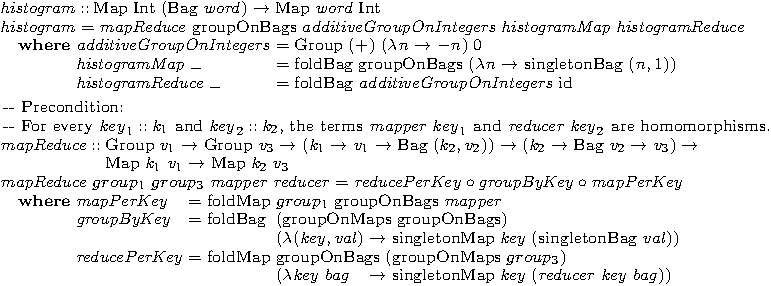
\includegraphics{pldi14/fig-mapReduce.pdf}
\caption{The $\Gl$-term $\HISTOGRAM$ with Haskell-like syntactic
  sugar. $\Term{additiveGroupOnIntegers}$ is the abelian group induced on
  integers by addition $(\mathbb{Z}, +, 0, -)$.}
\label{fig:case-study-pseudocode}
\end{figure*}

  
For base types with no known incrementalization strategy,
the precise interfaces for differentiation and
proof plugins can guide the implementation effort. These
interfaces could also from the basis for a library of
differentiation plugins that work well together.

Rewriting whole programs in our language would be an excessive
requirements. Instead, we embed our object language as an EDSL in
some more expressive meta-language (Scala in our case study), so
that embedded programs are reified. The embedded language can be
made to resemble the metalanguage~\citep{rompf2010lightweight}.
To incrementalize a part of a computation, we write it in our
embedded object language, invoke $\DERIVE$ on the embedded
program, optionally optimize the resulting programs and finally
invoke them. The metalanguage also acts as a macro system for the
object language, as usual. This allows us to simulate polymorphic
collections such as $\Bag*[\Gi]$ even though the object language is
simply-typed; technically, our plugin exposes a family of base
types to the object language.

\pg{Explain how we construct changes? The metalanguage can then
  construct changes in different ways?}



  \begin{oldSec}
\subsection{Methodology}
\label{ssec:methodology}


\begin{itemize}
\item We identify (classes of) base types which are relevant for
  our application, together with any relevant equational properties.
\item We define change representations for these base
  types.
\pg{Here we should give some criteria, if we can.}
\pg{For instance, restrictions on change structures which are
  erased become additional invariant for the change types.}
\pg{For instance, we should
  discuss the point of this paragraph:
``Furthermore, derivatives need to inspect the intensional
structure of changes, which are typically small, without applying
them to their base value, which is typically big. The interface
to do this depends on the specific change structure, hence we
specify no generic operation to allow this.''
}
\item We design for each (class of) base type a relevant set of
  primitives.  Where
  useful, we provide optimized derivatives for such primitives.
  We try to define primitives which capture
  incrementalizable computation skeletons; if such primitives are
  not general enough, we can add additional primitives which are
  more general but whose derivatives are less efficient.
\item We transform target programs to use our primitives.
\end{itemize}

\pg{I need self-maintainability and predicting nil changes here
  to discuss the example. So maybe the example should just be
  part of the case study.}
For instance, \citet{GlucheGrust97Incr} incrementalize bags for a
first-order language. By adapting/extending those techniques, we
can integrate bags into our higher-order language.

\pg{We should say dictionary, not map, for reduced ambiguity with the map operation.}
Using similar techniques, we also implemented support for the
operation on maps needed in our case study.

\pg{This section should also explain where changes come from.}
\end{oldSec}



\subsection{Predicting nil changes}
Handling changes to all inputs can induce excessive overhead in incremental
programs~\citep{Acar09}. It is also often
unnecessary; for instance, the function argument of $\Term{fold}$ in 
\cref{sec:intro} does not change since it is a closed subterm of the program, so
$\Term{fold}$ will receive a nil change for it.
A (conservative) static analysis can detect changes that are guaranteed to be nil at runtime. 
We can then specialize derivatives that receive this change, so that they need not
inspect the change at runtime.

For our case study, we have implemented a simple static analysis which
detects and propagates information about closed terms. The analysis is not interesting and 
we omit details for lack of space.



% Emacs, this is -*- latex -*-!

\subsection{Self-maintainability}
\label{sec:performance-cons}
\label{ssec:self-maint}

\begin{oldSec}
On its own, deriving $\Gl$-abstractions, applications and
variables (\cref{fig:correctness:derive}) does not improve performance.
It only relates the computations embodied in the primitives in
an incremental and higher-order setting, and provides a method to
generalize the vast quantity of research on first-order incremental
computation in the field of databases.
Our first approach toward performance gain is based on the idea of \emph{self-maintainable uses of primitives};
other approaches are certainly feasible. We did not formalize the
optimizations or prove them correct.
\end{oldSec}

In databases, a self-maintainable view~\citep{Gupta99MMV} is a function that can
update its result from input changes alone, without looking at
the actual input. By analogy, we call a derivative
\emph{self-maintainable} if it uses no
base parameters, only their changes. Self-maintainable derivatives
describe efficient incremental computations: since they do not
use their base input, their running time does not have to depend on the input
size.

\begin{examples}
$\Derive{\MERGE} = \Lam {x\; \D x\; y \; \D y}{\Merge{\D x}{\D y}}$
is self-maintainable with the
change structure $\ChangeStruct{\Bag{S}}$ described in
\cref{ssec:change-structures}, because it does not use the base
inputs $x$ and $y$.
Other derivatives are self-maintainable only in certain contexts.
The derivative of element-wise function application
$\App*{\App\MAP f}{\mathit{xs}}$ ignores the original
value of the bag $\mathit{xs}$ if the changes to
%
$f$ are always nil, because the underlying primitive $\FOLDBAG$
is self-maintainable in this case (as discussed in next section).
%
We take advantage of this by implementing a specialized
derivative for $\FOLDBAG$.

We have seen in \cref{ssec:differentiation} that $\Derivative$
needlessly recomputes $\Merge\Xs\Ys$. However, the result is a
base input to $\FOLD'$.
%
In next section, we'll replace $\FOLD'$ by a self-maintainable
derivative (based again on $\FOLDBAG$) and will avoid this
recomputation.
\end{examples}

%% Rationale for previous statement. Too complicated; left out.
%deriving a closed term without primitives yields a term that is
%self-maintainable whenever its higher-order arguments receive
%self-maintainable changes.
%The default rule $\Derive{c} = \Diff c c$ does not yield
%self-maintainable derivatives, because $\DIFF$ and $\APPLY$ use
%the input~$x$ in a significant way (\cref{fig:diff-apply}).
%However,

To conservatively predict whether a derivative is going to be
self-maintainable (and thus efficient), one can inspect whether
the program restricts itself to (conditionally) self-maintainable
primitives, like $\MERGE$ (always) or $\MAP \APP f$ (only if $\D
f$ is nil, which is guaranteed when $f$ is a closed term).

%% From the author response.
%It is possible to give a conservative approximation of whether a program's derivative is self-maintainable:
%If the original program only uses primitives with fully
%self-maintainable derivatives, the derivative of the program will
%be self-maintainable, too. We can syntactically approximate full
%self-maintainability of a primitive by checking whether the code
%of its derivative uses the $x$ variable (in addition to $\D x$) \pg{bind x! What about multiple arguments?}. For
%instance, the derivative of $\MERGE$ uses only $\D x$ and $\D y$, never $x$
%or $y$, and is hence fully self-maintainable. The derivative of
%$\FOLDBAG$ uses both $f$ and $\D f$; it is only self-maintainable
%sometimes (when df is the nil change).

\begin{oldSec}
Sometimes we can safely replace the derivative of a primitive by
a self-maintainable term, in which case we call it a
\emph{self-maintainable use of a primitive.}
Terms have self-maintainable derivatives if they use
primitives in a self-maintainable manner.

\pg{As Klaus points out, this is not true until we fix the set of
  changes - discussed in \#265. So we should specify the set of
  changes, or use a different example. We should also motivate
  it.}
%
\pg{Agreed: Convert to bags and to our running example, using foldBag.}
To illustrate, suppose $\MAP$ is a primitive of sets of
integers,
and changes to sets consist of insertions and deletions only.
The term
\[
\Lam x {\MapT {\Lam*n {n + 1}} x}
\]
contains a self-maintainable use of $\MAP$, because any change to
the input set~$x$, say $\{\App\INSERT5, \App\DELETE7\}$, can be
converted to an output change, say $\{\App\INSERT6,
\App\DELETE8\}$, without looking at $x$ itself. The use of $\MAP$
in the following term is not self-maintainable:
\[
\Lam x {\MapT {\Lam*n {n + \Sum* x}} x}.
\]
Even one insertion to the input set~$x$ generates a sweeping
change over all elements of the output set that is impossible to
express in terms of insertions and deletions without knowledge of $x$.

\pg{Before this, show that some of our primitives are
  self-maintainable, and some are self-maintainable if some
  inputs are nil.}
Our prototype optimization framework proceeds in two steps.
\begin{enumerate}
\item A static analysis identifies when changes are guaranteed to be nil.
\item During the differentiation transformation, $\DERIVE$
selects an appropriate self-maintainable function whenever possible,
considering the results of the static analysis.
\end{enumerate}
Due to space constraint, we cannot go into details of those
steps.
%
\yc{link to code}
%
\end{oldSec}

To avoid recomputing base arguments for self-maintainable derivatives
(which never need them), we
currently employ lazy evaluation.  Since we could use standard techniques for dead-code
elimination~\citep{Appel97} instead, laziness is not central to our
approach.

A significant restriction is that not-self-maintainable derivatives can require expensive computations to supply their base
arguments, which can be expensive to compute. Since they are also
computed while running the base program, one could reuse the previously
computed value through memoization or extensions of static
caching (as discussed in \cref{ssec:staticmemo}). We leave implementing these optimizations for future work. As a consequence,
our current implementation delivers good results only if
most derivatives are self-maintainable.

\begin{oldSec} % ID=Appel97
\pg{Do not remove without universal agreement. I don't think the paper can avoid discussing this aspect. }
One important issue is left. In a call-by-value
implementation of lambda calculus, running the program
\[
\Derive{\App{s}{t}} = \App{\App{\Derive{s}}{t}}{\Derive{t}}
\]
computes $t$
again, even though it was computed in the base program, thus
leading to wasteful repeated computation.
However, we claim this is a simpler problem to solve.
Three possibilities arise:
\begin{enumerate}
\item $t$ is very cheap to compute (for instance, it is a
  literal), so the problem does not occur.
\item $t$ is passed to a function which does not use it, hence
  we can avoid computing it using separate optimization steps, by
  executing the derivative with a lazy semantics (as done in our
  benchmarks) or (we expect) by using known techniques for
  interprocedural dead-code elimination~\citep{Appel97}.
\item Otherwise, since the term $t$
  was already computed while running the base
  program, we can save its value for use in the derivative.
  Approaches to
  implement this include memoization~\pg{cite} and extensions of
  static caching (as discussed in Sec.~\ref{sec:rw}).
  We leave investigating the different
  approaches to future work.
\end{enumerate}
\end{oldSec}

\begin{oldSec} % ID=Gupta99MMV
We next analyze when $t$ is going to be unused.
Inspecting the definition of $\DERIVE$ shows that only derivatives of (functions
containing) primitives can use $t$. For instance,
$\Derive{\Lam{x}{x}} = \Lam{x}{\Lam{\D x}{\D x}}$ does not use its
base input $x$, because $\Derive{x} = \D x$.
\pg{Make this more tentative. Remove 'prove'.}
It's easy to prove
by induction that if derivatives of primitives appearing in $s$
do not use their base input, neither does $s$.\footnote{Function
  changes coming from outside the program are not covered by this
  proof and are possible counterexamples.}

We term primitives whose derivative does not use their base input
self-maintainable, by analogy with the database concept of
self-maintainable views~\citep{Gupta99MMV}. \ko{Give example of 
self-maintainable and non-self-maintainable primitive}. 
We then extend this to programs: a
closed program is self-maintainable if its result does not depend
on base inputs or base intermediate results.
%
For programs which do not depend on functions as parameters (and
whose derivatives hence do not have function changes as
parameters), it should be straightforward to prove that being
self-maintainable is equivalent to only using self-maintainable
primitives.

Hence, we can argue informally that if a program only uses
self-maintainable primitives, its derivative will not recompute
base intermediate results (except if they are computed for
unrelated reasons). In our case study (Sec.~\ref{sec:eval}),
such derivatives are already
extremely efficient.

\pg{This should be somehow better integrated in the rest of the section.}
\end{oldSec}


\subsection{Case study}
\label{sec:plugins}


We perform a case study on a nontrivial realistic program to
demonstrate that \ILC\ can speed it up.
We take the MapReduce-based skeleton of the
word-count example~\citep{Lammel07}. We define a
suitable differentiation plugin, adapt the program to use it and show
that incremental computation is faster than recomputation.
%
We designed and implemented the differentiation plugin 
following the requirements of the corresponding proof plugin,
even though we did not formalize
the proof plugin (e.g. in Agda).
For lack of space, we focus on base types
which are crucial for our example and its performance, that is,
collections.
%
The plugin also implements tuples, tagged unions, Booleans and
integers with the usual introduction and elimination forms, with
few optimizations for their derivatives.

$\WORDCOUNT$ takes a map
from document IDs to documents and produces a map
from words appearing in the input to the count of their
appearances, that is, a histogram:
\[
\HasType \WORDCOUNT {\Fun {\HashMap \DOCUMENTID \DOCUMENT} {\HashMap \WORD \Int}}
\]
For simplicity, instead of modeling strings, we model documents
as bags of words and document IDs as integers. Hence, what we implement is:
\[
\HasType \HISTOGRAM {\Fun {\HashMap \Int {\Bag*[a]}} {\HashMap a \Int}}
\]
We model words by integers ($a = Int$), but treat them parametrically.
Other than that, we adapt directly
\citeauthor{Lammel07}'s code to our language.
\pg{But it cannot accept all the same parameters... Ah, but it
  depends on which foldMap we call. OK.}
\Cref{fig:case-study-pseudocode} shows the $\Gl$-term
$\HISTOGRAM$.

% Emacs, this is -*- latex -*-!
\begin{figure}

\centering

\lstinputlisting[language=scala,
firstline=10,
escapechar=|,
literate=
{=>}{$\Rightarrow\,$}2
{>=}{$\ge\;$}2
{<-}{$\leftarrow\;$}2
{!=}{$\ne\;$}2
{Abelian-group-based}{\text{Abelian-group-based }}1
{<}{$<$}2
{bag1}{{bag$_1$}}4
{bag2}{{bag$_2$}}4
{value1}{{value$_1$}}6
{value2}{{value$_2$}}6
{dict1}{{dict$_1$}}5
{dict2}{{dict$_2$}}5
{v1}{{v$_1$}}2
{v2}{{v$_2$}}2
{???}{$\ldots$}3
]{pldi14/mapReduce.scala}
\caption[A Scala implementation of primitives for bags and maps]{A Scala implementation of primitives for bags and maps.
In the code, we call $\boxplus$, $\boxminus$ and $e$ respectively \emph{merge}, \emph{inverse}, and \emph{zero}.
We also omit the relatively standard primitives.\pg{Can we now move this code to an appendix, since we explain so much in text?}}
\label{fig:primitives}
\end{figure}


\pg{Why does 'target language' show up all of a sudden? Shouldn't
  we say that we generate Scala code for execution
  \textbf{elsewhere}? Right now, we say it in next section. Confusing.}
%
\Cref{fig:primitives} shows a simplified
Scala implementation of the primitives
used in \cref{fig:case-study-pseudocode}.
As bag primitives, we provide constructors and a fold operation,
following \citet{GlucheGrust97Incr}. The constructors for bags
are $\Empty$ (constructing the empty bag), $\SINGLETON$
(constructing a bag with one element), $\MERGE$ (constructing the
merge of two bags) and $\NEGATE$ ($\Negate{b}$ constructs a bag
with the same elements as $b$ but negated multiplicities); all but $\SINGLETON$ represent
abelian group operations.
%
Unlike for usual ADT constructors, the same bag can be
constructed in different ways, which are equivalent by the equations defining abelian groups;
for instance, since $\MERGE$ is commutative, $\Merge{x}{y} = \Merge{y}{x}$.
%
Folding on a bag will represent the bag through constructors in
an arbitrary way, and then replace constructors with arguments;
to ensure a well-defined result, the arguments of fold should
respect the same equations, that is, they should form an abelian group;
for instance, the binary operator should be commutative.
%
Hence, the fold operator $\FOLDBAG$ can be defined to take a
function (corresponding to $\SINGLETON$) and an abelian group
(for the other constructors). $\FOLDBAG$ is then defined by equations:
%
\begin{alignat*}{2}
&  \HasType{\FOLDBAG}{\mathbf{Group}\; \Gt \to (\Gs \to \Gt) \to &&\Bag[\Gs] \to \Gt}\\
&  \App{\FoldBag {g @ (\_, \boxplus, \boxminus, e)}{f}}{\Empty}
    &&= e \displaybreak[0]\\
&  \App{\FoldBag {g @ (\_, \boxplus, \boxminus, e)}{f}}{\Merge* {b_1} {b_2}}
   &&= \App{\FoldBag{g}{f}}{b_1} \displaybreak[0]\\
&&& \boxplus
  \App{\FoldBag{g}{f}}{b_1} \displaybreak[0]\\
&  \App{\FoldBag {g @ (\_, \boxplus, \boxminus, e)}{f}}{\Negate* b}
   && = \boxminus \; \App*{\FoldBag{g}{f}}{b}\displaybreak[0]\\
&  \App{\FoldBag {g @ (\_, \boxplus, \boxminus, e)}{f}}{\Singleton*{v}}
   &&= \App{f}{v}
\end{alignat*}
%
If $g$ is a group,
these equations specify $\App{\FOLDBAG} g$ precisely~\citep{GlucheGrust97Incr}.
%
Moreover, the first three equations mean that $\FoldBag{g}{f}$ is \emph{abelian group
  homomorphism} between the abelian group on bags and the group
$g$ (because those equations coincide with the definition).
%
\Cref{fig:primitives} shows an implementation of $\FOLDBAG$ as
specified above.
Moreover, all functions which deconstruct a bag can be expressed in
terms of $\FOLDBAG$ with suitable arguments.
%
For instance, we can sum the elements of a bag of integers with
$\FoldBag{\Term{gZ}}{\Lam*{x}{x}}$, where
$\Term{gZ}$ is the abelian group on integers defined in
\cref{ssec:change-structures}.
Users of $\FOLDBAG$ can define different abelian groups to specify
different operations (for instance, to multiply floating-point numbers).

If $g$ and $f$ do not change, $\FoldBag{g}{f}$ has a self-maintainable
derivative.
By the equations above,
\pg{Non-standard alignment, because the last line doesn't fit.}
\begin{align*}
& \FoldBag{g}{f} \Update*{b}{\D b}\displaybreak[0]\\
=\;& \FoldBag{g}{f} {(\Merge b {\D b})}\\
=\;& \App{\FoldBag{g}{f}}{b}  \boxplus \App{\FoldBag{g}{f}}{\D b} \\
=\;& \Update{\App{\FoldBag{g}{f}}{b}}{\Term{GroupChange} \; g \; \left(\App{\FoldBag{g}{f}}{\D b}\right)}
\end{align*}
We will describe the $\Term{GroupChange}$ change constructor in a moment.
Before that, we note that as a consequence, the derivative of $\FoldBag{g}{f} $ is
\[
\Lam{b \; db} \Term{GroupChange} \; g \; \left(\App{\FoldBag{g}{f}}{\D b}\right)\text{,}
\]
and we can see it does not use $b$: as desired, it is
\emph{self-maintainable}. Additional restrictions are require to
make $\FOLDMAP$'s derivative self-maintainable. Those restrictions require the
precondition on $\Term{mapReduce}$ in
\cref{fig:case-study-pseudocode}. $\Term{foldMapGen}$ has the
same implementation but without those restrictions; as a
consequence, its derivative is not self-maintainable, but it is more generally applicable.
Lack of space prevents us from giving more details.

To define $\Term{GroupChange}$, we need a suitable erased change
structure on $\Gt$, such that $\UPDATE$ will be equivalent to
$\boxplus$. Since there might be multiple groups on $\Gt$, we
\emph{allow the changes to specify a group}, and have
$\UPDATE$ delegate to $\boxplus$:
\begin{align*}
& \Change{\Gt} = \Term{Replace}\; \Gt \mid \Term{GroupChange} \Abelian*{\Gt} \Gt \\
& \Update{v}{(\Term{Replace} \; u)} = u\\
& \Update{v}{(\Term{GroupChange} \; (\bullet, \Term{inverse}, \Term{zero})\; dv)} = v \bullet dv\\
& \Diff{v}{u} = \Term{Replace}\; v
\end{align*}
That is, a change between two values is either simply the new
value (which replaces the old one, triggering recomputation),
or their difference (computed with abelian group
operations, like in the changes structures for groups from
\cref{ssec:change-structures}. The operator $\DIFF$
does not know which group to use, so it does not take advantage
of the group structure.
However, $\FOLDBAG$ is now able to generate a group change.
% Rewrite:
%derivatives of primitives like $\FOLDBAG$ can
%use the group structure they have available when producing changes.
%
\pg{Clarify about user-defined groups.}

We rewrite $\Program$ in terms of $\FOLDBAG$ to take advantage of
group-based changes.
{\DeriveProgramEnv
\begin{align*}
&\Term{id}=\Lam{x}{x}\\
&G_+ = (\mathbb Z, +, -, 0)\\
&\Program = \Lam{\Xs}{\Lam{\Ys}{\FOLDBAG~G_+~\Term{id}~(\Merge\Xs\Ys)}}\\
&\Derive\Program=\\
&\zero
\Lam{\Xs}{\Lam{\DXs}{}}\Lam{\Ys}{\Lam{\DYs}{}}\\
&\one
\FOLDBAG'~G_+~G_+'~\Term{id}~\Term{id}'\\
&\two
(\Merge\Xs\Ys)\\
&\two
(\MERGE'~\Xs~\DXs~\Ys~\DYs)
\end{align*}
}%
It is now possible to write down the derivative of $\FOLDBAG$.
{\DeriveProgramEnv
\begin{align*}
&\text{(if static analysis detects that $\D G$ and $\D f$
are nil changes)}\\
&\FOLDBAG'=\Derive{\FOLDBAG}=\\
&\zero
\Lam{G}{\Lam{\D G}{\Lam{f}{\Lam{\D f}{
\Lam{\Zs}{\Lam{\DZs}{}}}}}}\\
&\one
\Term{GroupChange}~G~
(\FOLDBAG~G~f~\DZs)
\end{align*}
}%
We know from \cref{ssec:plugin} that
\[
\MERGE'=\Lam{u}{\Lam{\D u}{\Lam{v}{\Lam{\D v}{\Merge{\D u}{\D v}}}}}.
\]
Inlining $\FOLDBAG'$ and $\MERGE'$ gives us a more readable term
$\beta$-equivalent to the derivative of $\Program$:
{\DeriveProgramEnv
\begin{align*}
&\Derive\Program=\\
&\zero
\Lam{\Xs}{\Lam{\DXs}{}}\Lam{\Ys}{\Lam{\DYs}{}}
%
\FOLDBAG~G_+~\Term{id}~
(\MERGE~\DXs~\DYs).
\end{align*}
}%

\begin{oldSec}
Function destructing bags must be homomorphisms between abelian
groups~\citep{GlucheGrust97Incr}, and can all be defined in terms
of $\FOLDBAG$. More in general, bags form an abelian
\emph{collection group}.
%
%To incrementalize bags, we reuse the change structure on bags
%described in \cref{ssec:change-structures}.
%
An abelian group on $\Gi$ can be lifted to an abelian collection
group on $(\HashMap{\kappa}{\Gi})$ through \emph{mapGroup}, so that we
can apply similar ideas to maps. The resulting primitives for map
are expressive enough to efficiently incrementalize our example
program.

Destructing an abelian collection group produces a value in an
abelian group (such as integers or abelian collection groups). To
avoid hardcoding which group to use, we define a general change
structure for abelian groups. After erasure, the change structure is as follows
(cf.~\cref{fig:change-operations,fig:case-study-pseudocode}):\footnote{For clarity, we use ADTs and pattern matching instead of sum types.}
...

The derivative of $\App{\FOLDBAG}{f}$ is efficient on $\Term{Update}$ changes when $df$ is
known to be a nil change; in that case,
$\App{\FOLDBAG}{f}$ is a homomorphism, hence self-maintainable (\cref{sec:performance-cons}). To see why, take any homomorphism $\HasType f {\Fun \Gs \Gt}$ 
between user-defined
abelian groups $G_\Gs$ and $G_\Gt$, and suppose
$\D v = \HasType{\Term{Update} \; (G_\Gs, u)}{\Change \Gs}$. By homomorphism properties,
\begin{align*}
\App f {\Update*{v}{\D v}}
&= \App f {(v \bullet_\Gs u)}
= \App* f v  \bullet_\Gt \App* f u \\
&= \Update{\App* f v}{\Term{Update} \;(G_\Gt, \App f u)}.
\end{align*}
The derivative of $f$ on
$\Term{Update}$ changes is then $\App{\App{f'}{v}}{(\Term{Update} \; (G_\Gs, u))} = \Term{Update} \; (G_\Gt, \App f u)$,
by \cref{def:derivatives}.
$f'$
requires no information about $v$, therefore it is
self-maintainable. That is the
principle behind all derivatives in the plugin that are faster
than recomputation.
\end{oldSec}

\begin{oldSec}
\subsubsection{Bags}

We apply \citeauthor{GlucheGrust97Incr}'s approach to view
maintenance based on monoid- and group-homomorphisms
\citep{GlucheGrust97Incr}. An operation $f$ on a collection is
effectively incrementalized if the collection type forms a group
$G$, and $f$ is a homomorphism from $G$ to some group over its
result type. Bags with signed multiplicities%
%
\footnote{Bags with signed multiplicities correspond to databases
described in \citet{Koch10IQE}, where tuples are allowed to have
negative multiplicities. Bag elements with negative
multiplicities represent deletion of themselves.}
%
form the free abelian group over their element type; their nice
properties are particularly suitable for our purposes.
Incremental computation based on noncommutative groups requires
caching intermediate results, and we leave it for future work.

Bag constructors $\Empty$, $\SINGLETON$, $\MERGE$ are identical
to those used in \citet{GlucheGrust97Incr}. We add a primitive
$\NEGATE$ to create bags with negative multiplicities.
% listing order follows argument order of $\FOLDBAG$.
\begin{align*}
\HasTypeAligned{\MERGE}
  {\Fun{\Fun{\Bag[\Gi]}{\Bag[\Gi]}}{\Bag[\Gi]}}
\\
\HasTypeAligned{\NEGATE}
  {\Fun{\Gi}{\Bag[\Gi]}}
\\
\HasTypeAligned{\Empty}
  {\Bag[\Gi]}
\\
\HasTypeAligned{\SINGLETON}
  {\Fun{\Gi}{\Bag[\Gi]}}
\end{align*}
If we consider $\NEGATE$ to be another bag constructor, then a
natural elimination form of bags is the primitive $\FOLDBAG$:
\begin{align*}
\HasTypeAligned\FOLDBAG
  {\Fun {\Abelian \Gi}
    {\Fun {\Fun*{\Gi}{\Gt}} {\Gt}}}
\\
\Abelian\Gi
  & =      \Fun*{\Base\Gi}{\Fun{\Base\Gi}{\Base\Gi}} \\
  & \times \Fun*{\Base\Gi}{\Base\Gi} \\
  & \times \Base*\Gi.
\end{align*}
\citet{GlucheGrust97Incr} implement many object query language
views in terms of $\FOLDBAG$ to show that they are
homomorphisms and easily incrementalized. Since our framework
supports higher-order functions, we can actually offer
$\FOLDBAG$ to users, who are then free to write all kinds of
easily incrementalized homomorphisms
(\cref{foldBag-homomorphism}).

% Actually, the fact & lemma below talk about functions in the
% semantic domain. Semantic brackets are left out by abusing
% notation.
\begin{definition}[Semantics of bag primitives]~
\begin{subdefinition}
\item $\Eval{\Bag[\Gi]}$ is the free abelian group with basis $\Eval\Gi$.
\item $\MERGE$ evaluates to the binary operator of the free abelian
group.
\item $\NEGATE$ evaluates to the function that takes every
element of $\Eval{\Bag[\Gi]}$ to its inverse in the free abelian
group.
\item $\Empty$ evaluates to the identity element of the free
abelian group.
\item\label{foldBag-homomorphism} If
$\HasType{G_\tau}{\Abelian\tau}$ evaluates to an abelian group,
then for every term $\HasType f {\Fun\Gi\Gt}$, the term
$\App*{\App\FOLDBAG{G_\tau}}{f}$ evaluates to the unique
homomorphism%
\footnote{ The universal property of free abelian groups
guarantees the existence and uniqueness of such a homomorphism. A
constructive proof of the universal property doubles as a
specification of $\FOLDBAG$. } %
from the free abelian group on $\Gi$ to the group denoted by
$G_\tau$.
\end{subdefinition}
\end{definition}

\subsubsection{Maps}

There is no obvious abelian group structure on maps as there is
on bags. However, $\HashMap\Gk\Gi$ can be thought of as (possibly
infinite) vectors over nullable values of type $\Gi$ indexed by
all values of type $\Gk$. It suggests the group structure on maps
as an indexed direct product of a group structure on $\Gi$. The
formulation would be more elegant if there were dependent type
support in the object language.

These are the primitives on maps.
\begin{align*}
\HasTypeAligned\MAKEMAP
  {\Fun\Gk{\Fun\Gi{\HashMap\Gk\Gi}}}
\\
\HasTypeAligned\LOOKUP
  {\Fun\Gk{\Fun{\Map\Gk\Gi}{\Maybe\Gi}}}
\\
\HasTypeAligned\LIFTGROUP
  \Fun{\Abelian\Gi}{\Abelian{\HashMap\Gk\Gi}}
\\
\HasTypeAligned\FOLDMAP
  \Fun{\Abelian\Gi}
    {\Fun{\Abelian\Gt} \\ & \qquad
      {\Fun{ \Fun*\Gk{\Fun\Gi\Gt} }
        {\Fun{\HashMap\Gk\Gi} \Gt}}}
\end{align*}

\begin{definition}[Semantics of map primitives]~
\begin{subdefinition}
\item $\Eval{\Map\Gk\Gi}$ is the set of partial functions from
$\Eval\Gk$ to $\Eval\Gi$ defined only at a finite number of
points.
\item $\MAKEMAP$ evaluates to the function that converts a
key-value pair to the corresponding partial function defined at
1 point.
\item $\LOOKUP$ evaluates to the standard lookup function on
maps.
\item $\LIFTGROUP$ evaluates to a function that maps abelian
groups $G_\Gi$ over $\Eval\Gi$ to the abelian group formed by
direct product of copies of $G_\Gi$ indexed by $\Eval\Gk$. Its
identity element, binary operation and inverse function are the
empty map, map merge and map negation.
\item Given a map $\HasType m {\HashMap\Gk\Gi}$, abelian groups
$G_\Gi$, $G_\Gt$, and a function $\HasType f
{\Fun\Gk{\Fun\Gi\Gt}}$ such that $\App*fk$ is a homomorphism from
$G_\Gi$ to $G_\Gt$ for every $\HasType k\Gk$, the term
\[
\App{\App{\App{\App\FOLDMAP{G_\Gi}}{G_\Gt}}f}m
\]
evaluates to a value in $\Eval\Gt$ by the following steps (we
write $m(k)$ for the value of the map $m$ at key $k$).
\begin{enumerate}
\item Replace each $m(k)$ by $\App*{\App fk}{m(k)}$ to create the
map $\HasType{m'}{\HashMap\Gk\Gt}$.
\item Sum all values of $m'$ by the binary operation of $G_\Gt$.
\end{enumerate}
Since both steps are homomorphisms,
$\App*{\App{\App\FOLDMAP{G_\Gi}}{G_\Gt}}f$ is a homomorphism
from $\App*\LIFTGROUP{G_\Gi}$ to $G_\Gt$.
% to the unique homomorphism%
% \footnote{The existence and uniqueness of such a homomorphism is
% guaranteed by the universal property of indexed direct product
% as a product in the category of abelian groups.} %
% from $\App*\LIFTGROUP{G_\Gi}$ to $G_\Gt$ that agrees with
% $\App*fk$ for every $\HasType k \Gk$.
%
\end{subdefinition}
\end{definition}

Since our object language lacks dependent types, the user has to
make sure that the higher-order argument of $\FOLDMAP$ gives
rise to homomorphisms. This is the price paid for the
expressivity of user-defined groups.

\end{oldSec}
% Below are previous formulations.

% OLDSEC: rephrased skeleton & pointers
\begin{oldSec}
We perform a case study applying our technique to a MapReduce
skeleton. To this end, we implemented in Scala a language plugin
supporting some collections. We restricted ourselves to
primitives whose derivatives could be made self-maintainable.

To this end, we recast and extend some ideas by
\citet{GlucheGrust97Incr} and \citet{Koch10IQE} in our framework.
The collections we consider are maps and bags with negative
multiplicities. We use negative multiplicites to represent
removal of elements.%
%
\footnote{Our framework allows having standard bags as base types
  and bags with negative multiplicities as their change type. We
  leave this and a few other extension for future work.}
%
Bag elements must be comparable for equality, and this excludes
functions. Moreover, storing functions in data is hard because
the derivative of code extracting and using the function must
also have access to the derivative of that function. We plan to
augment base programs to also store function derivatives together
with the functions, but leave this for future work. \pg{Say
  something more.}

\pg{Write instantiation for bags.}
\begin{figure}[h]
\begin{align*}
\Change[\Bag \iota]{b} & = \Bag \iota\\
\Diff[\Bag \iota]{x}{y} & = \Merge x {\Negate*y}\\[\eqsep]
\Apply[\Bag \iota]{\D x}{x} & = \Merge x y
\end{align*}
%\caption{Term difference and change application.}
%\label{fig:plug-diff-apply}
\end{figure}
\end{oldSec}

% OLDSEC: skeleton.
% Refer for ideas.
\begin{oldSec}
We will illustrate a fully instantiated differentiation framework
by the simplest plugin expressive enough for nontrivial
applications. We will not prove the properties required of the
plugin for correctness to hold, but we believe that they are
true.

We designed the plugin around abelian groups.
Abelian groups are good for incrementalizing folds over a
collection because the irrelevance of folding order and the
possibility of removing an element from the fold via its inverse
means that we don't have to save any intermediate result. We
shall not investigate the caching aspect of incrementalization;
we do it later.

Some base types have changes based on abelian groups. Other base
types (sums) don't, but are still useful. Our plugin does not
make everything efficient. We give some primitives fast
derivatives now, and plan to support more and more primitives to
allow more and more fast derivatives.

By the way, we forbid functions in collections because nil
changes to functions have computation content and can't be
discarded. [Illustrating example: Klaus's f]

\subsection*{Details}

Listing: base types, their change types, DIFF, UPDATE

Those fall into 2 categories: those whose change we don't care
about (simply use replacement), and those whose change we care
about (change is either replacement value, or user-supplied
abelian group together with a group element.

Listing: derivatives

We can talk about foldBag and foldMap alone, leaving
everything else the difference with itself (that is, stupid
derivative by recomputation).
\end{oldSec}

% OLDSEC: abelian groups
% Refer to it when discussing AbelianDerivation traits.
\begin{oldSec}
Our approach is parametric in the concrete representation of
changes of type $\Change{\tau}$ as long as changes support the
operations listed in \cref{fig:change-operations}).
The update operator $\Apply{\D x}{x}$ updates a value $x$ with a
change $\D x$. The difference operator $\Diff{y}{x}$ computes the
change from $x$ to $y$.
And the nil change operator $\Nil{x}$
denotes the change that updates the value $x$ into itself.

In fact, if $\tau$ forms a group $\langle \tau, 0, +, -\rangle$,
we can define $\Diff{v_2}{v_1} = v_2 + (- v_1)$; for some groups,
we can use the resulting definition for incremental computation
\pg{not clear what this means yet}, as we will see later.
However, many interesting datatypes do not form groups, such as
functions or lists (\citet{GlucheGrust97Incr} introduce a group
structure for lists, but it is too restrictive\pg{elaborate});
hence we introduce here a more general abstraction, which can be
implemented via groups \pg{reorder this with the previous
  paragraph}.

\pg{I write $\cdot-\cdot$ for a binary operation, but I need something better.}
For instance, we can take $\tau$ to be the set of integers $\bz$. Integers are
the support of the commutative group $(\bz, \cdot + \cdot, 0, -\cdot)$, hence they are equipped
with a difference operation $\cdot-\cdot = \Gl x y. x + (-y)$. We can thus represent
changes for relative numbers with relative numbers: $\Diff{v_2}{v_1} = v_2 -
v_1$.

More formally, take an arbitrary type $\tau$ and values $v_1, v_2$ of
these type. We can describe the difference between these two values
with $\D v = \Diff{v_2}{v_1}$: this evaluates to a change $\D v$ which is
valid for $v_1$. Moreover, we can apply \pg{is this the term to use?} this change to a value
with $\Apply{\D v}v$. We have the guarantee that
$\Apply{\left(\Diff{v_2}{v_1}\right)}{v_1} = v_2$. In general, if we
apply changes to values for which they are not valid, our axioms do
not specify the result. Moreover, our axioms for arbitrary base types
only guarantee that a change $\Diff{v_2}{v_1}$ is valid for $v_1$,
even though, for many implementations of changes, $\Diff{v_2}{v_1}$ is
valid for values other than $v_1$. This is the case in particular if
the base type forms a group and we define changes reusing this group
structure, as we did for integers. In interesting applications, however, changes
are not generated directly by $\DIFF$.

Moreover, if $\D v$ is a valid change, we also have
$\Diff{\left(\Apply{\D v}v\right)}v = \D v$.

Our presentation of the behavior of changes on a datatype forms
an algebraic specification (excluding the concept of validity and
the properties which only apply to valid changes). In particular,
we can define a signature having sorts $\tau$ and $\Change{\tau}$,
the functions from \cref{fig:change-operations}
and equations (or axioms):
\begin{align*}
\Apply{\Diff*{s₂}{s₁}}{s₁} &= s₂\\
\Apply{\Nil{s}}{s} &= s\\
\end{align*}
\pg{Check which ones we have already proven.}

Since this set of axioms is algebraic (that is, purely first
order), we know from universal algebra~\citep{Mitchell1996foundations} that equational reasoning
is sound and complete for all models (implementations) of this
algebraic specification.

Moreover, we can show that those axioms are consistent by
providing models implementing them. \pg{Resume}
%Additionally, we have two implementations of those axioms.
\pg{A couple more axioms need to be checked.}
%
% (s₂ ⊝ (ds ⊕ s₁)) ∘ ds &= s₂ ⊝ s₁ (?)
%
% Special case:
%	(ds ⊕ s) ⊝ s = ds (EDIT: only if ds is valid for s).
%
% Therorems:
%
%s ⊝ s = nil s
%(s₁ ⊝ s₂) ∘ (s₂ ⊝ s₃) = s₁ ⊝ s₃
\end{oldSec}

\subsection{Benchmark results}

Our results show (\cref{fig:graph}) that our program reacts to input changes
in essentially constant time, as expected, hence orders of magnitude faster than
recomputation. Constant factors are small enough that the speedup is apparent on realistic input sizes.

For lack of space, details on benchmarking results and inputs
are available in the extended version of our paper (Appendix A).

Two important lessons from the evaluations are:
\begin{itemize}
\item As anticipated in \cref{ssec:self-maint}, to achieve good performance our current
  implementation requires some form of dead code elimination, such as laziness.
%Either laziness or dead-code elimination is required for
%good performance ().
\item Incrementalization increases code size significantly.
  Analyzing and addressing this increase is left for future work.
\end{itemize}

\begin{figure}
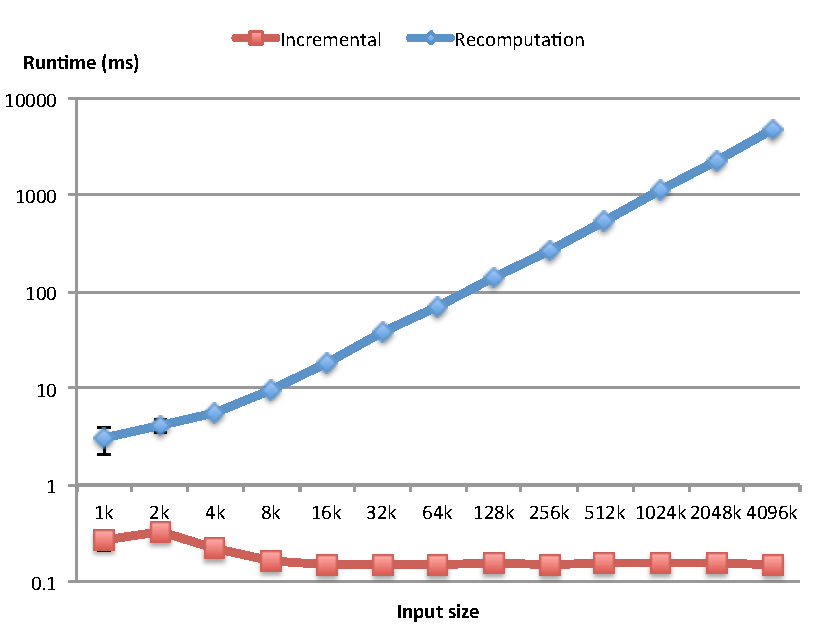
\includegraphics[keepaspectratio,width=8.5cm]{pldi14/HistogramGenerated-new.pdf}
\caption{Performance results in log-log scale, with input size on
  the x-axis and runtime in ms on the y-axis. Confidence
  intervals are shown by the whiskers; most whiskers are
  too small to be visible.}
\label{fig:graph}
\end{figure}


% Emacs, this is -*- latex -*-!
\chapter{Related work}
\label{sec:rw}

Existing work on incremental computation can be divided into two
groups: Static incrementalization and dynamic incrementalization.
Static approaches analyze a program statically and generate an incremental
version of it. Dynamic approaches create dynamic dependency graphs while
the program runs and propagate changes along these graphs.

The trade-off between the two is that static approaches have the potential
to be faster because no dependency tracking at runtime is needed, whereas
dynamic approaches can support more expressive programming languages.
%
\ILC\ is a static approach, but compared to the other static
approaches it supports more expressive languages.

In the remainder of this section, we analyze the relation to the
most closely related prior works. \Citet{Ramalingam93}, \citet{Gupta99MMV}
and \citet{Acar06} discuss further related work.


\section{Dynamic approaches}
One of the most advanced dynamic approach to incrementalization is
self-adjusting computation, which has been applied to Standard ML
and large subsets of C~\citep{Acar09,Hammer11}.
In this approach, programs execute on the original
input in an enhanced runtime environment that tracks the
dependencies between values in a \emph{dynamic
  dependence graph}~\citep{Acar06}; intermediate results are
memoized.
Later, changes to the input propagate through
dependency graphs from changed inputs to results,
updating both intermediate and final results;
this processing is often more efficient than recomputation.

However, creating dynamic
dependence graphs imposes a large constant-factor overhead during
runtime, ranging from 2 to 30 in reported
experiments~\citep{Acar09EAS,Acar10TDT}, and affecting the
initial run of the program on its base input.
\citet{Acar10TDT} show how to support high-level data
types in the context of self-adjusting computation; however, the
approach still requires expensive runtime bookkeeping during the initial run.
Our approach, like other static ones, uses a standard runtime
environment and has no overhead
during base computation, but may be less efficient when processing
changes. This pays off if the initial input is 
big compared to its changes.


\citet{Chen11} have developed a static transformation for purely
functional programs, but this transformation just provides a superior interface to use
the runtime support with less boilerplate, and does not reduce
this performance overhead. Hence, it is still a dynamic approach, unlike
the transformation this work presents.

Another property of self-adjusting computation
is that incrementalization is only efficient if the program has a suitable
computation structure. For instance, a program
folding the elements of a bag with a left or right fold will not
have efficient incremental behavior; instead, it's necessary that
the fold be shaped like a balanced tree. In general,
incremental computations become efficient only if they are \emph{stable}~\citep{Acar05}.
Hence one may need to massage the program to make it efficient. Our methodology is 
different: Since we do not aim to incrementalize arbitrary programs written in standard
programming languages, we can select primitives that have efficient derivatives and thereby require 
the programmer to use them.

Functional reactive programming \citep{Elliott:1997:FRA:258948.258973}
can also be seen as a dynamic approach to incremental computation;
recent work by \citet{Maier2013} has
focused on speeding up reactions to input changes by making them
incremental on collections. \citet{Willis08} use dynamic techniques
 to incrementalize JQL queries.

\section{Static approaches}
\pg{If we discuss partial evaluation, we should compare to
  \citep{Sundaresh91}}
Static approaches analyze a program at compile-time and produce an
incremental version that efficiently updates the output
of the original program according to changing inputs.

Static approaches have the potential to be more efficient than dynamic approaches,
because no bookkeeping at runtime is required. Also, the computed incremental
versions can often be optimized using standard compiler techniques
such as constant folding or inlining.
However, none of them support first-class functions; some
approaches have further restrictions.

Our aim is to apply static incrementalization to more expressive languages;
in particular, \ILC\ supports first-class functions and an open
set of base types with associated primitive operations.

\subsection{Finite differencing}
\label{sec:finite-diff}
\citet{Paige82FDC} present derivatives for a first-order language
with a fixed set of primitives.
\citet{Blakeley:1986:EUM} apply these ideas to a class of relational queries.
The database community extended
this work to queries on relational data, such as in \emph{algebraic
  differencing}~\citep{Gupta99MMV}, which inspired our work and
terminology. However, most of this work does not apply to nested
collections or algebraic data types, but only to relational
(flat) data, and no previous approach handles first-class
functions. Incremental support is typically designed
monolithically for a whole language, rather than piecewise.
Improving on algebraic differencing, \citet{Koch10IQE}
\emph{guarantees} asymptotic speedups with a compositional query
transformation and delivers huge speedup in realistic benchmarks,
though still for a first-order database language.
\pg{continue with new work, discuss why we don't do iterated differentiation.}

More general (non-relational) data types are considered in the work by \citet{GlucheGrust97Incr};
our support for bags and the use of groups is inspired by their work,
but their architecture is still rather restrictive: they lack
support for function changes and restrict incrementalization to
self-maintainable views, without hinting at a possible solution.

\subsection{Static memoization}
\label{ssec:staticmemo}
\citeauthor{Liu00}'s work~\citep{Liu00} allows to incrementalize a first-order base
program $f(\Old{x})$ to compute $f(\New{x})$, knowing how
$\New{x}$ is related to $\Old{x}$. To this end, they transform
$f(\New{x})$ into an incremental program which reuses the
intermediate results produced while computing $f(\Old{x})$, the
base program. To this end, (i) first the base program is
transformed to save all its intermediate results, then (ii) the
incremental program is transformed to reuse those intermediate
results, and finally (iii) intermediate results which are not
needed are pruned from the base program. However, to reuse
intermediate results, the incremental program must often be
rearranged, using some form of equational reasoning, into some
equivalent program where partial results appear literally. For
instance, if the base program $f$ uses a left fold to sum the
elements of a list of integers $\Old{x}$, accessing them from the
head onwards, and $\New{x}$ prepends a new element $h$ to the
list, at no point does $f(\New{x})$ recompute the same results.
But since addition is commutative on integers, we can rewrite
$f(\New{x})$ as $f(\Old{x}) + h$. The author's CACHET system will
try to perform such rewritings automatically, but it is not
guaranteed to succeed. Similarly, CACHET will try to synthesize
any additional results which can be computed cheaply by the base
program to help make the incremental program more efficient.

Since it is hard to fully automate such reasoning, we move
equational reasoning to the plugin design phase. A 
plugin provides general-purpose higher-order primitives for which
the plugin authors have devised efficient derivatives (by using
equational reasoning in the design phase). Then, the
differentiation algorithm computes incremental
versions of user programs without requiring further user intervention.
It would be useful to combine \ILC\ with some form of static
caching to make the computation of derivatives which
are not self-maintainable more efficient. We plan to do so
in future work.
%Our approach is instead fully automatic, and will always produce
%a result, which in the worst case will merely be slow;
%% they can also fail and then 'produce a slow program'.
%
%we envision the use of directed rewrite rules for further
%optimization of programs, instead of undirected search.
%% Not so important.

\chapter{Conclusion}
\label{ssec:future}
In this part we have presented \ILC, an approach to lifting incremental computations
on first-order programs to incremental computations on higher-order
programs. We have presented a machine-checked correctness proof 
of a formalization of \ILC\ and an initial experimental evaluation
in the form of an implementation, a sample plugin for maps and bags,
and a non-trivial example that was incrementalized successfully and
efficiently. 

\pg{Revise}
Our work opens several avenues of future work. Our current implementation
is not efficient on derivatives that are not self-maintainable.
However, as discussed
(Sec.~\ref{ssec:self-maint}), we will study how
to memoize intermediate results to address this limitation. Our next
step will be to develop language plugins which
have efficient non-self-maintainable primitives.

Another area of future work is adding support for algebraic data
types (including recursive types), polymorphism, subtyping, general recursion
and other collection types. While support for algebraic data
types could subsume support for specific collections, many
collections have additional algebraic properties that enable faster
incrementalization (like bags). Even lists (which have fewer algebraic properties)
can benefit from special support~\citep{Maier2013}.

Moreover, we intend to apply \ILC{} to optimize queries on
collections in the context of the \textsc{SQuOpt}
project~\citep{GiarrussoAOSD13}, which was a motivation for this
work; in particular, \textsc{SQuOpt} can automatically rewrite
queries to use database-style indexes, and \ILC{} enables
updating those indexes when input data changes.

\begin{oldSec}
Our derivatives accept arbitrary changes for all inputs. We plan
to stage the code that updates the inputs through lightweight
modular staging~\citep{rompf2010lightweight}, analyze it to
predict changes and specialize the derivative to the result of
this analysis. For instance, if we need to update $\Term{f} \;
\Term{bag}$ after $\Term{bagNew} = \Term{insert} \; \Term{el} \;
\Term{bagOld}$, we can infer that $\Term{dbag}$ is an insertion
and specialize $f'$ to such a change.
\end{oldSec}

Finally, we intend to perform a full and thorough experimental evaluation
to demonstrate that \ILC\ can incrementalize large-scale practical programs.


\part{Static caching}
\label{part:caching}
\chapter{POPL}
\newcommand{\poplPath}[1]{popl18/#1}
% Emacs, this is -*- latex -*-!
%% ODER: format ==         = "\mathrel{==}"
%% ODER: format /=         = "\neq "
%
%
\makeatletter
\@ifundefined{lhs2tex.lhs2tex.sty.read}%
  {\@namedef{lhs2tex.lhs2tex.sty.read}{}%
   \newcommand\SkipToFmtEnd{}%
   \newcommand\EndFmtInput{}%
   \long\def\SkipToFmtEnd#1\EndFmtInput{}%
  }\SkipToFmtEnd

\newcommand\ReadOnlyOnce[1]{\@ifundefined{#1}{\@namedef{#1}{}}\SkipToFmtEnd}
\usepackage{amstext}
\usepackage{amssymb}
\usepackage{stmaryrd}
\DeclareFontFamily{OT1}{cmtex}{}
\DeclareFontShape{OT1}{cmtex}{m}{n}
  {<5><6><7><8>cmtex8
   <9>cmtex9
   <10><10.95><12><14.4><17.28><20.74><24.88>cmtex10}{}
\DeclareFontShape{OT1}{cmtex}{m}{it}
  {<-> ssub * cmtt/m/it}{}
\newcommand{\texfamily}{\fontfamily{cmtex}\selectfont}
\DeclareFontShape{OT1}{cmtt}{bx}{n}
  {<5><6><7><8>cmtt8
   <9>cmbtt9
   <10><10.95><12><14.4><17.28><20.74><24.88>cmbtt10}{}
\DeclareFontShape{OT1}{cmtex}{bx}{n}
  {<-> ssub * cmtt/bx/n}{}
\newcommand{\tex}[1]{\text{\texfamily#1}}	% NEU

\newcommand{\Sp}{\hskip.33334em\relax}


\newcommand{\Conid}[1]{\mathit{#1}}
\newcommand{\Varid}[1]{\mathit{#1}}
\newcommand{\anonymous}{\kern0.06em \vbox{\hrule\@width.5em}}
\newcommand{\plus}{\mathbin{+\!\!\!+}}
\newcommand{\bind}{\mathbin{>\!\!\!>\mkern-6.7mu=}}
\newcommand{\rbind}{\mathbin{=\mkern-6.7mu<\!\!\!<}}% suggested by Neil Mitchell
\newcommand{\sequ}{\mathbin{>\!\!\!>}}
\renewcommand{\leq}{\leqslant}
\renewcommand{\geq}{\geqslant}
\usepackage{polytable}

%mathindent has to be defined
\@ifundefined{mathindent}%
  {\newdimen\mathindent\mathindent\leftmargini}%
  {}%

\def\resethooks{%
  \global\let\SaveRestoreHook\empty
  \global\let\ColumnHook\empty}
\newcommand*{\savecolumns}[1][default]%
  {\g@addto@macro\SaveRestoreHook{\savecolumns[#1]}}
\newcommand*{\restorecolumns}[1][default]%
  {\g@addto@macro\SaveRestoreHook{\restorecolumns[#1]}}
\newcommand*{\aligncolumn}[2]%
  {\g@addto@macro\ColumnHook{\column{#1}{#2}}}

\resethooks

\newcommand{\onelinecommentchars}{\quad-{}- }
\newcommand{\commentbeginchars}{\enskip\{-}
\newcommand{\commentendchars}{-\}\enskip}

\newcommand{\visiblecomments}{%
  \let\onelinecomment=\onelinecommentchars
  \let\commentbegin=\commentbeginchars
  \let\commentend=\commentendchars}

\newcommand{\invisiblecomments}{%
  \let\onelinecomment=\empty
  \let\commentbegin=\empty
  \let\commentend=\empty}

\visiblecomments

\newlength{\blanklineskip}
\setlength{\blanklineskip}{0.66084ex}

\newcommand{\hsindent}[1]{\quad}% default is fixed indentation
\let\hspre\empty
\let\hspost\empty
\newcommand{\NB}{\textbf{NB}}
\newcommand{\Todo}[1]{$\langle$\textbf{To do:}~#1$\rangle$}

\EndFmtInput
\makeatother
%
%
%
%
%
%
% This package provides two environments suitable to take the place
% of hscode, called "plainhscode" and "arrayhscode". 
%
% The plain environment surrounds each code block by vertical space,
% and it uses \abovedisplayskip and \belowdisplayskip to get spacing
% similar to formulas. Note that if these dimensions are changed,
% the spacing around displayed math formulas changes as well.
% All code is indented using \leftskip.
%
% Changed 19.08.2004 to reflect changes in colorcode. Should work with
% CodeGroup.sty.
%
\ReadOnlyOnce{polycode.fmt}%
\makeatletter

\newcommand{\hsnewpar}[1]%
  {{\parskip=0pt\parindent=0pt\par\vskip #1\noindent}}

% can be used, for instance, to redefine the code size, by setting the
% command to \small or something alike
\newcommand{\hscodestyle}{}

% The command \sethscode can be used to switch the code formatting
% behaviour by mapping the hscode environment in the subst directive
% to a new LaTeX environment.

\newcommand{\sethscode}[1]%
  {\expandafter\let\expandafter\hscode\csname #1\endcsname
   \expandafter\let\expandafter\endhscode\csname end#1\endcsname}

% "compatibility" mode restores the non-polycode.fmt layout.

\newenvironment{compathscode}%
  {\par\noindent
   \advance\leftskip\mathindent
   \hscodestyle
   \let\\=\@normalcr
   \let\hspre\(\let\hspost\)%
   \pboxed}%
  {\endpboxed\)%
   \par\noindent
   \ignorespacesafterend}

\newcommand{\compaths}{\sethscode{compathscode}}

% "plain" mode is the proposed default.
% It should now work with \centering.
% This required some changes. The old version
% is still available for reference as oldplainhscode.

\newenvironment{plainhscode}%
  {\hsnewpar\abovedisplayskip
   \advance\leftskip\mathindent
   \hscodestyle
   \let\hspre\(\let\hspost\)%
   \pboxed}%
  {\endpboxed%
   \hsnewpar\belowdisplayskip
   \ignorespacesafterend}

\newenvironment{oldplainhscode}%
  {\hsnewpar\abovedisplayskip
   \advance\leftskip\mathindent
   \hscodestyle
   \let\\=\@normalcr
   \(\pboxed}%
  {\endpboxed\)%
   \hsnewpar\belowdisplayskip
   \ignorespacesafterend}

% Here, we make plainhscode the default environment.

\newcommand{\plainhs}{\sethscode{plainhscode}}
\newcommand{\oldplainhs}{\sethscode{oldplainhscode}}
\plainhs

% The arrayhscode is like plain, but makes use of polytable's
% parray environment which disallows page breaks in code blocks.

\newenvironment{arrayhscode}%
  {\hsnewpar\abovedisplayskip
   \advance\leftskip\mathindent
   \hscodestyle
   \let\\=\@normalcr
   \(\parray}%
  {\endparray\)%
   \hsnewpar\belowdisplayskip
   \ignorespacesafterend}

\newcommand{\arrayhs}{\sethscode{arrayhscode}}

% The mathhscode environment also makes use of polytable's parray 
% environment. It is supposed to be used only inside math mode 
% (I used it to typeset the type rules in my thesis).

\newenvironment{mathhscode}%
  {\parray}{\endparray}

\newcommand{\mathhs}{\sethscode{mathhscode}}

% texths is similar to mathhs, but works in text mode.

\newenvironment{texthscode}%
  {\(\parray}{\endparray\)}

\newcommand{\texths}{\sethscode{texthscode}}

% The framed environment places code in a framed box.

\def\codeframewidth{\arrayrulewidth}
\RequirePackage{calc}

\newenvironment{framedhscode}%
  {\parskip=\abovedisplayskip\par\noindent
   \hscodestyle
   \arrayrulewidth=\codeframewidth
   \tabular{@{}|p{\linewidth-2\arraycolsep-2\arrayrulewidth-2pt}|@{}}%
   \hline\framedhslinecorrect\\{-1.5ex}%
   \let\endoflinesave=\\
   \let\\=\@normalcr
   \(\pboxed}%
  {\endpboxed\)%
   \framedhslinecorrect\endoflinesave{.5ex}\hline
   \endtabular
   \parskip=\belowdisplayskip\par\noindent
   \ignorespacesafterend}

\newcommand{\framedhslinecorrect}[2]%
  {#1[#2]}

\newcommand{\framedhs}{\sethscode{framedhscode}}

% The inlinehscode environment is an experimental environment
% that can be used to typeset displayed code inline.

\newenvironment{inlinehscode}%
  {\(\def\column##1##2{}%
   \let\>\undefined\let\<\undefined\let\\\undefined
   \newcommand\>[1][]{}\newcommand\<[1][]{}\newcommand\\[1][]{}%
   \def\fromto##1##2##3{##3}%
   \def\nextline{}}{\) }%

\newcommand{\inlinehs}{\sethscode{inlinehscode}}

% The joincode environment is a separate environment that
% can be used to surround and thereby connect multiple code
% blocks.

\newenvironment{joincode}%
  {\let\orighscode=\hscode
   \let\origendhscode=\endhscode
   \def\endhscode{\def\hscode{\endgroup\def\@currenvir{hscode}\\}\begingroup}
   %\let\SaveRestoreHook=\empty
   %\let\ColumnHook=\empty
   %\let\resethooks=\empty
   \orighscode\def\hscode{\endgroup\def\@currenvir{hscode}}}%
  {\origendhscode
   \global\let\hscode=\orighscode
   \global\let\endhscode=\origendhscode}%

\makeatother
\EndFmtInput
%
% Emacs, this is -*- latex -*-!

%
%
% First, let's redefine the forall, and the dot.
%
%
% This is made in such a way that after a forall, the next
% dot will be printed as a period, otherwise the formatting
% of `comp_` is used. By redefining `comp_`, as suitable
% composition operator can be chosen. Similarly, period_
% is used for the period.
%
\ReadOnlyOnce{forall.fmt}%
\makeatletter

% The HaskellResetHook is a list to which things can
% be added that reset the Haskell state to the beginning.
% This is to recover from states where the hacked intelligence
% is not sufficient.

\let\HaskellResetHook\empty
\newcommand*{\AtHaskellReset}[1]{%
  \g@addto@macro\HaskellResetHook{#1}}
\newcommand*{\HaskellReset}{\HaskellResetHook}

\global\let\hsforallread\empty

\newcommand\hsforall{\global\let\hsdot=\hsperiodonce}
\newcommand*\hsperiodonce[2]{#2\global\let\hsdot=\hscompose}
\newcommand*\hscompose[2]{#1}

\AtHaskellReset{\global\let\hsdot=\hscompose}

% In the beginning, we should reset Haskell once.
\HaskellReset

\makeatother
\EndFmtInput


% https://github.com/conal/talk-2015-essence-and-origins-of-frp/blob/master/mine.fmt
% Complexity notation:






% If an argument to a formatting directive starts with let, lhs2TeX likes to
% helpfully prepend a space to the let, even though that's seldom desirable.
% Write lett to prevent that.













































% Hook into forall.fmt:
% Add proper spacing after forall-generated dots.











% We shouldn't use /=, that means not equal (even if it can be overriden)!







% XXX



%  format `stoup` = "\blackdiamond"






% Cancel the effect of \; (that is \thickspace)



% Use as in |vapply vf va (downto n) v|.
% (downto n) is parsed as an application argument, so we must undo the produced
% spacing.

% indexed big-step eval
% without environments
% big-step eval
% change big-step eval








% \, is 3mu, \! is -3mu, so this is almost \!\!.


\def\deriveDefCore{%
\begin{align*}
  \ensuremath{\Derive{\lambda (\Varid{x}\typcolon\sigma)\to \Varid{t}}} &= \ensuremath{\lambda (\Varid{x}\typcolon\sigma)\;(\Varid{dx}\typcolon\Delta \sigma)\to \Derive{\Varid{t}}} \\
  \ensuremath{\Derive{\Varid{s}\;\Varid{t}}} &= \ensuremath{\Derive{\Varid{s}}\;\Varid{t}\;\Derive{\Varid{t}}} \\
  \ensuremath{\Derive{\Varid{x}}} &= \ensuremath{\Varid{dx}} \\
  \ensuremath{\Derive{\Varid{c}}} &= \ensuremath{\DeriveConst{\Varid{c}}}
\end{align*}
}


% Drop unsightly numbers from function names. The ones at the end could be
% formatted as subscripts, but not the ones in the middle.




\section{Introduction}

Incremental computation is often desirable: after computing an output from some
input, we often need to produce new outputs corresponding to changed inputs. One
can simply rerun the same \emph{base program} on the new input; but instead,
incremental computation transforms the input change to an output change. This
can be desirable because more efficient.

Incremental computation could also be desirable because the changes themselves
are of interest: Imagine a typechecker explaining how some change to input
source propagates to changes to the typechecking result. More generally, imagine
a program explaining how some change to its input propagates through a
computation into changes to the output.

ILC (Incremental $\lambda$-Calculus)~\citep{CaiEtAl2014ILC} is
a recent approach to incremental computation for higher-order languages.
ILC represents changes from an old value \ensuremath{\Varid{v}_{1}} to an updated value \ensuremath{\Varid{v}_{2}} as a
first-class value written \ensuremath{\Varid{dv}}. ILC also transforms statically \emph{base programs}
to \emph{incremental programs} or \emph{derivatives}: derivatives produce
output changes from changes to all their inputs. Since functions are first-class
values, ILC introduces a notion of function changes.

However, as mentioned by \citeauthor{CaiEtAl2014ILC} and as we explain below,
ILC as currently defined does not allow reusing intermediate results created by the
base computation during the incremental computation. That restricts ILC to
supporting efficiently only \emph{self-maintainable computations}, a rather
restrictive class: for instance, mapping self-maintainable functions on a sequence is
self-maintainable, but dividing numbers isn't! In this paper, we remove this
limitation.

% non-blinded
% In this paper, we address this restriction as we promised in previous work.
%In keeping with our approach, we try to avoid forcing unnecessary overhead onto
%the computation.

To remember intermediate results, many incrementalization approaches rely on
forms of memoization: one uses hashtables to memoize function results, or
dynamic dependence graphs~\citep{Acar05} to remember the computation trace.
However, such data structures often remember results that might not be reused;
moreover, the data structures themselves (as opposed to their values) occupy
additional memory, looking up intermediate results has a cost in time, and
typical general-purpose optimizers cannot predict results from memoization
lookups. Instead, ILC aims to produce purely functional programs that are
suitable for further optimizations.

We eschew memoization: instead, we transform programs to
\emph{cache-transfer style (CTS)}, following ideas from \citet{Liu95}. CTS functions
output \emph{caches} of intermediate results along with their primary results. Caches
are just nested tuples whose structure is derived from code, and accessing them
does not involve looking up keys depending on inputs. We also extend
differentiation to produce \emph{CTS derivatives}, which can extract from caches
any intermediate results they need.
%\pg{they can also extract inputs, but I can't explain it here.}
This approach was inspired and pioneered by \citeauthor{Liu95} for untyped
first-order functional languages, but we integrate
it with ILC and extend it to higher-order typed languages.

% \pg{we don't!}
%and then use program transformation techniques to eliminate unneeded state.
%
While CTS functions still produce additional intermediate data structures,
produced programs can be subject to further optimizations.
We believe static analysis of a CTS function and its CTS derivative can identify
and remove unneeded state (similar to what has been done by \citeauthor{Liu95}),
as we discuss in \cref{sec:cache-pruning}.
We leave a more careful analysis to future work.

We prove most of our formalization correct in Coq
To support non-simply-typed programs, all our proofs
are for untyped $\lambda$-calculus, while previous ILC correctness proofs were
restricted to simply-typed $\lambda$-calculus.
Unlike previous ILC proofs, we simply define which changes are valid
via a \emph{logical relation}, then show the fundamental property for this
logical relation (see \cref{sec:ilc-background}). To extend this proof to
untyped $\lambda$-calculus, we switch to \emph{step-indexed} logical relations.

To support differentiation on our case studies, we also represent function changes
as closures that can be inspected, to support manipulating them more efficiently
and detecting at runtime when a function change is \emph{nil} hence need not be
applied. To show this representation is correct, we also use closures in our
mechanized proof.

Unlike plain ILC, typing programs in CTS is challenging, because the shape of
caches for a function depends on the function implementation.
Our case studies show how to non-trivially embed resulting programs in typed
languages, at least for our case studies, but our proofs support an untyped
target language.

In sum, we present the following contributions:
\pg{revise more, add sections; this is getting redundant with the text.}
\begin{itemize}
\item via examples, we motivate extending ILC to remember intermediate
  results (\cref{sec:cts-motivation});
\item we give a novel proof of correctness for ILC for untyped
  $\lambda$-calculus, based on step-indexed logical relations
  (\cref{sec:sound-derive});
\item building on top of ILC-style differentiation, we show how to transform
  untyped higher-order programs to \emph{cache-transfer-style}~(CTS)~%
  (\cref{sec:transformation});
\item we show that programs and derivatives in cache-transfer style
  \emph{simulate} correctly their non-CTS variants (\cref{sec:transformation-soundness});
\item we mechanize in Coq most of our proofs%
\begin{poplForPopl}
% PG: I'm commenting this out, assuming that we fix this soon
%, save for a few straightforward lemmas
 (see supplementary material)%
\end{poplForPopl}
;
\item we perform performance case studies (in \cref{sec:case-studies}) applying
  (by hand) extension of this technique to Haskell programs, and incrementalize
  efficiently also programs that do not admit self-maintainable derivatives.
\end{itemize}

\pg{Try merging with contributions if we can.}
The rest of the paper is organized as follows. \Cref{sec:cts-motivation} summarizes
ILC and motivates the extension to cache-transfer style.
\Cref{sec:formalization} presents our formalization and proofs.
\iftoggle{poplForThesis}{
\Cref{sec:case-studies} presents our case studies and benchmarks.
\Cref{sec:cts-limitations} discusses limitations and future work.
}{
\Cref{sec:case-studies} discusses our case studies, benchmarks,
limitations and future work.
}
\Cref{sec:cts-rw}
discusses related work and \cref{sec:conclusions} concludes.

% Emacs, this is -*- latex -*-!
%% ODER: format ==         = "\mathrel{==}"
%% ODER: format /=         = "\neq "
%
%
\makeatletter
\@ifundefined{lhs2tex.lhs2tex.sty.read}%
  {\@namedef{lhs2tex.lhs2tex.sty.read}{}%
   \newcommand\SkipToFmtEnd{}%
   \newcommand\EndFmtInput{}%
   \long\def\SkipToFmtEnd#1\EndFmtInput{}%
  }\SkipToFmtEnd

\newcommand\ReadOnlyOnce[1]{\@ifundefined{#1}{\@namedef{#1}{}}\SkipToFmtEnd}
\usepackage{amstext}
\usepackage{amssymb}
\usepackage{stmaryrd}
\DeclareFontFamily{OT1}{cmtex}{}
\DeclareFontShape{OT1}{cmtex}{m}{n}
  {<5><6><7><8>cmtex8
   <9>cmtex9
   <10><10.95><12><14.4><17.28><20.74><24.88>cmtex10}{}
\DeclareFontShape{OT1}{cmtex}{m}{it}
  {<-> ssub * cmtt/m/it}{}
\newcommand{\texfamily}{\fontfamily{cmtex}\selectfont}
\DeclareFontShape{OT1}{cmtt}{bx}{n}
  {<5><6><7><8>cmtt8
   <9>cmbtt9
   <10><10.95><12><14.4><17.28><20.74><24.88>cmbtt10}{}
\DeclareFontShape{OT1}{cmtex}{bx}{n}
  {<-> ssub * cmtt/bx/n}{}
\newcommand{\tex}[1]{\text{\texfamily#1}}	% NEU

\newcommand{\Sp}{\hskip.33334em\relax}


\newcommand{\Conid}[1]{\mathit{#1}}
\newcommand{\Varid}[1]{\mathit{#1}}
\newcommand{\anonymous}{\kern0.06em \vbox{\hrule\@width.5em}}
\newcommand{\plus}{\mathbin{+\!\!\!+}}
\newcommand{\bind}{\mathbin{>\!\!\!>\mkern-6.7mu=}}
\newcommand{\rbind}{\mathbin{=\mkern-6.7mu<\!\!\!<}}% suggested by Neil Mitchell
\newcommand{\sequ}{\mathbin{>\!\!\!>}}
\renewcommand{\leq}{\leqslant}
\renewcommand{\geq}{\geqslant}
\usepackage{polytable}

%mathindent has to be defined
\@ifundefined{mathindent}%
  {\newdimen\mathindent\mathindent\leftmargini}%
  {}%

\def\resethooks{%
  \global\let\SaveRestoreHook\empty
  \global\let\ColumnHook\empty}
\newcommand*{\savecolumns}[1][default]%
  {\g@addto@macro\SaveRestoreHook{\savecolumns[#1]}}
\newcommand*{\restorecolumns}[1][default]%
  {\g@addto@macro\SaveRestoreHook{\restorecolumns[#1]}}
\newcommand*{\aligncolumn}[2]%
  {\g@addto@macro\ColumnHook{\column{#1}{#2}}}

\resethooks

\newcommand{\onelinecommentchars}{\quad-{}- }
\newcommand{\commentbeginchars}{\enskip\{-}
\newcommand{\commentendchars}{-\}\enskip}

\newcommand{\visiblecomments}{%
  \let\onelinecomment=\onelinecommentchars
  \let\commentbegin=\commentbeginchars
  \let\commentend=\commentendchars}

\newcommand{\invisiblecomments}{%
  \let\onelinecomment=\empty
  \let\commentbegin=\empty
  \let\commentend=\empty}

\visiblecomments

\newlength{\blanklineskip}
\setlength{\blanklineskip}{0.66084ex}

\newcommand{\hsindent}[1]{\quad}% default is fixed indentation
\let\hspre\empty
\let\hspost\empty
\newcommand{\NB}{\textbf{NB}}
\newcommand{\Todo}[1]{$\langle$\textbf{To do:}~#1$\rangle$}

\EndFmtInput
\makeatother
%
%
%
%
%
%
% This package provides two environments suitable to take the place
% of hscode, called "plainhscode" and "arrayhscode". 
%
% The plain environment surrounds each code block by vertical space,
% and it uses \abovedisplayskip and \belowdisplayskip to get spacing
% similar to formulas. Note that if these dimensions are changed,
% the spacing around displayed math formulas changes as well.
% All code is indented using \leftskip.
%
% Changed 19.08.2004 to reflect changes in colorcode. Should work with
% CodeGroup.sty.
%
\ReadOnlyOnce{polycode.fmt}%
\makeatletter

\newcommand{\hsnewpar}[1]%
  {{\parskip=0pt\parindent=0pt\par\vskip #1\noindent}}

% can be used, for instance, to redefine the code size, by setting the
% command to \small or something alike
\newcommand{\hscodestyle}{}

% The command \sethscode can be used to switch the code formatting
% behaviour by mapping the hscode environment in the subst directive
% to a new LaTeX environment.

\newcommand{\sethscode}[1]%
  {\expandafter\let\expandafter\hscode\csname #1\endcsname
   \expandafter\let\expandafter\endhscode\csname end#1\endcsname}

% "compatibility" mode restores the non-polycode.fmt layout.

\newenvironment{compathscode}%
  {\par\noindent
   \advance\leftskip\mathindent
   \hscodestyle
   \let\\=\@normalcr
   \let\hspre\(\let\hspost\)%
   \pboxed}%
  {\endpboxed\)%
   \par\noindent
   \ignorespacesafterend}

\newcommand{\compaths}{\sethscode{compathscode}}

% "plain" mode is the proposed default.
% It should now work with \centering.
% This required some changes. The old version
% is still available for reference as oldplainhscode.

\newenvironment{plainhscode}%
  {\hsnewpar\abovedisplayskip
   \advance\leftskip\mathindent
   \hscodestyle
   \let\hspre\(\let\hspost\)%
   \pboxed}%
  {\endpboxed%
   \hsnewpar\belowdisplayskip
   \ignorespacesafterend}

\newenvironment{oldplainhscode}%
  {\hsnewpar\abovedisplayskip
   \advance\leftskip\mathindent
   \hscodestyle
   \let\\=\@normalcr
   \(\pboxed}%
  {\endpboxed\)%
   \hsnewpar\belowdisplayskip
   \ignorespacesafterend}

% Here, we make plainhscode the default environment.

\newcommand{\plainhs}{\sethscode{plainhscode}}
\newcommand{\oldplainhs}{\sethscode{oldplainhscode}}
\plainhs

% The arrayhscode is like plain, but makes use of polytable's
% parray environment which disallows page breaks in code blocks.

\newenvironment{arrayhscode}%
  {\hsnewpar\abovedisplayskip
   \advance\leftskip\mathindent
   \hscodestyle
   \let\\=\@normalcr
   \(\parray}%
  {\endparray\)%
   \hsnewpar\belowdisplayskip
   \ignorespacesafterend}

\newcommand{\arrayhs}{\sethscode{arrayhscode}}

% The mathhscode environment also makes use of polytable's parray 
% environment. It is supposed to be used only inside math mode 
% (I used it to typeset the type rules in my thesis).

\newenvironment{mathhscode}%
  {\parray}{\endparray}

\newcommand{\mathhs}{\sethscode{mathhscode}}

% texths is similar to mathhs, but works in text mode.

\newenvironment{texthscode}%
  {\(\parray}{\endparray\)}

\newcommand{\texths}{\sethscode{texthscode}}

% The framed environment places code in a framed box.

\def\codeframewidth{\arrayrulewidth}
\RequirePackage{calc}

\newenvironment{framedhscode}%
  {\parskip=\abovedisplayskip\par\noindent
   \hscodestyle
   \arrayrulewidth=\codeframewidth
   \tabular{@{}|p{\linewidth-2\arraycolsep-2\arrayrulewidth-2pt}|@{}}%
   \hline\framedhslinecorrect\\{-1.5ex}%
   \let\endoflinesave=\\
   \let\\=\@normalcr
   \(\pboxed}%
  {\endpboxed\)%
   \framedhslinecorrect\endoflinesave{.5ex}\hline
   \endtabular
   \parskip=\belowdisplayskip\par\noindent
   \ignorespacesafterend}

\newcommand{\framedhslinecorrect}[2]%
  {#1[#2]}

\newcommand{\framedhs}{\sethscode{framedhscode}}

% The inlinehscode environment is an experimental environment
% that can be used to typeset displayed code inline.

\newenvironment{inlinehscode}%
  {\(\def\column##1##2{}%
   \let\>\undefined\let\<\undefined\let\\\undefined
   \newcommand\>[1][]{}\newcommand\<[1][]{}\newcommand\\[1][]{}%
   \def\fromto##1##2##3{##3}%
   \def\nextline{}}{\) }%

\newcommand{\inlinehs}{\sethscode{inlinehscode}}

% The joincode environment is a separate environment that
% can be used to surround and thereby connect multiple code
% blocks.

\newenvironment{joincode}%
  {\let\orighscode=\hscode
   \let\origendhscode=\endhscode
   \def\endhscode{\def\hscode{\endgroup\def\@currenvir{hscode}\\}\begingroup}
   %\let\SaveRestoreHook=\empty
   %\let\ColumnHook=\empty
   %\let\resethooks=\empty
   \orighscode\def\hscode{\endgroup\def\@currenvir{hscode}}}%
  {\origendhscode
   \global\let\hscode=\orighscode
   \global\let\endhscode=\origendhscode}%

\makeatother
\EndFmtInput
%
% Emacs, this is -*- latex -*-!

%
%
% First, let's redefine the forall, and the dot.
%
%
% This is made in such a way that after a forall, the next
% dot will be printed as a period, otherwise the formatting
% of `comp_` is used. By redefining `comp_`, as suitable
% composition operator can be chosen. Similarly, period_
% is used for the period.
%
\ReadOnlyOnce{forall.fmt}%
\makeatletter

% The HaskellResetHook is a list to which things can
% be added that reset the Haskell state to the beginning.
% This is to recover from states where the hacked intelligence
% is not sufficient.

\let\HaskellResetHook\empty
\newcommand*{\AtHaskellReset}[1]{%
  \g@addto@macro\HaskellResetHook{#1}}
\newcommand*{\HaskellReset}{\HaskellResetHook}

\global\let\hsforallread\empty

\newcommand\hsforall{\global\let\hsdot=\hsperiodonce}
\newcommand*\hsperiodonce[2]{#2\global\let\hsdot=\hscompose}
\newcommand*\hscompose[2]{#1}

\AtHaskellReset{\global\let\hsdot=\hscompose}

% In the beginning, we should reset Haskell once.
\HaskellReset

\makeatother
\EndFmtInput


% https://github.com/conal/talk-2015-essence-and-origins-of-frp/blob/master/mine.fmt
% Complexity notation:






% If an argument to a formatting directive starts with let, lhs2TeX likes to
% helpfully prepend a space to the let, even though that's seldom desirable.
% Write lett to prevent that.













































% Hook into forall.fmt:
% Add proper spacing after forall-generated dots.











% We shouldn't use /=, that means not equal (even if it can be overriden)!







% XXX



%  format `stoup` = "\blackdiamond"






% Cancel the effect of \; (that is \thickspace)



% Use as in |vapply vf va (downto n) v|.
% (downto n) is parsed as an application argument, so we must undo the produced
% spacing.

% indexed big-step eval
% without environments
% big-step eval
% change big-step eval








% \, is 3mu, \! is -3mu, so this is almost \!\!.


\def\deriveDefCore{%
\begin{align*}
  \ensuremath{\Derive{\lambda (\Varid{x}\typcolon\sigma)\to \Varid{t}}} &= \ensuremath{\lambda (\Varid{x}\typcolon\sigma)\;(\Varid{dx}\typcolon\Delta \sigma)\to \Derive{\Varid{t}}} \\
  \ensuremath{\Derive{\Varid{s}\;\Varid{t}}} &= \ensuremath{\Derive{\Varid{s}}\;\Varid{t}\;\Derive{\Varid{t}}} \\
  \ensuremath{\Derive{\Varid{x}}} &= \ensuremath{\Varid{dx}} \\
  \ensuremath{\Derive{\Varid{c}}} &= \ensuremath{\DeriveConst{\Varid{c}}}
\end{align*}
}


% Drop unsightly numbers from function names. The ones at the end could be
% formatted as subscripts, but not the ones in the middle.




\section{Introducing Cache-Transfer Style}
\label{sec:cts-motivation}
In this section we motivate cache-transfer style (CTS).
\Cref{sec:ilc-background} summarizes a reformulation of ILC, so we recommend it
also to readers familiar with \citet{CaiEtAl2014ILC}.
In \cref{sec:motivating-example} we consider a minimal first-order example, namely an
average function. We incrementalize it using ILC, explain why the result is
inefficient, and show that remembering results via cache-transfer style enables
efficient incrementalization with asymptotic speedups.
In \cref{sec:higher-order-example} we consider a higher-order example that
requires not just cache-transfer style but also efficient support for both nil
and non-nil function changes, together with the ability to detect nil changes.

\subsection{Background}
\label{sec:ilc-background}
ILC considers simply-typed programs, and assumes that base types and primitives
come with support for incrementalization.

The ILC framework describes changes as first-class values, and types them using
dependent types. To each type \ensuremath{\Conid{A}} we associate a type \ensuremath{\Delta \Conid{A}} of changes for
\ensuremath{\Conid{A}}, and an \emph{update operator} \ensuremath{\oplus \mathrel{:\mkern-1mu:}\Conid{A}\to \Delta \Conid{A}\to \Conid{A}}, that updates an
initial value with a change to compute an updated value.
We also consider changes for evaluation environments, which contain changes for
each environment entry.

A change \ensuremath{\Varid{da}\mathrel{:\mkern-1mu:}\Delta \Conid{A}} can be \emph{valid} from \ensuremath{\Varid{a}_{1}\mathrel{:\mkern-1mu:}\Conid{A}} to \ensuremath{\Varid{a}_{2}\mathrel{:\mkern-1mu:}\Conid{A}}, and we write
then \ensuremath{\vvcreltau{\Varid{a}_{2}}{\Conid{A}}{\Varid{a}_{1}}{\Varid{da}}}. Then \ensuremath{\Varid{a}_{1}} is the \emph{source} or \emph{initial value}
for \ensuremath{\Varid{da}}, and \ensuremath{\Varid{a}_{2}} is the \emph{destination} or \emph{updated value} for \ensuremath{\Varid{da}}.
From \ensuremath{\vvcreltau{\Varid{a}_{2}}{\Conid{A}}{\Varid{a}_{1}}{\Varid{da}}} follows that \ensuremath{\Varid{a}_{2}} coincides with \ensuremath{\Varid{a}_{1}\oplus \Varid{da}}, but
validity imposes additional invariants that are useful during
incrementalization.
A change can be valid for more than one source, but a change \ensuremath{\Varid{da}} and a source
\ensuremath{\Varid{a}_{1}} uniquely determine the destination \ensuremath{\Varid{a}_{2}\mathrel{=}\Varid{a}_{1}\oplus \Varid{da}}.
To avoid ambiguity, we always consider a change together with a specific source.

Each type comes with its definition of validity: Validity is a ternary
\emph{logical relation}.
%
For function types \ensuremath{\Conid{A}\to \Conid{B}}, we
define \ensuremath{\Delta (\Conid{A}\to \Conid{B})\mathrel{=}\Conid{A}\to \Delta \Conid{A}\to \Delta \Conid{B}}, and say that
a function change \ensuremath{\Varid{df}\mathrel{:\mkern-1mu:}\Delta (\Conid{A}\to \Conid{B})} is valid from \ensuremath{\Varid{f}_{1}\mathrel{:\mkern-1mu:}\Conid{A}\to \Conid{B}} to \ensuremath{\Varid{f}_{2}\mathrel{:\mkern-1mu:}\Conid{A}\to \Conid{B}} (that is, \ensuremath{\vvcreltau{\Varid{f}_{2}}{\Conid{A}\to \Conid{B}}{\Varid{f}_{1}}{\Varid{df}}}) if and only if \ensuremath{\Varid{df}} maps valid input
changes to valid output changes; by that,
we mean that if \ensuremath{\vvcreltau{\Varid{a}_{2}}{\Conid{A}}{\Varid{a}_{1}}{\Varid{da}}}, then \ensuremath{\vvcreltau{\Varid{f}_{2}\;\Varid{a}_{2}}{\Conid{B}}{\Varid{f}_{1}\;\Varid{a}_{1}}{\Varid{df}\;\Varid{a}_{1}\;\Varid{da}}}.
Source and destination of \ensuremath{\Varid{df}\;\Varid{a}_{1}\;\Varid{da}}, that is \ensuremath{\Varid{f}_{1}\;\Varid{a}_{1}} and \ensuremath{\Varid{f}_{2}\;\Varid{a}_{2}}, are the result of
applying two different functions, that is \ensuremath{\Varid{f}_{1}} and \ensuremath{\Varid{f}_{2}}.

\pg{Rewritten to generalize ``derivative''.}
ILC expresses incremental programs as \emph{derivatives}. Generalizing previous
usage, we simply say derivative for all terms produced by differentiation.
If \ensuremath{\Varid{dE}} is a valid environment change from \ensuremath{\Conid{E}_{1}} to \ensuremath{\Conid{E}_{2}}, and term \ensuremath{\Varid{t}} is
well-typed and can be evaluated against environments \ensuremath{\Conid{E}_{1},\Conid{E}_{2}},
then term \ensuremath{\iderive{\Varid{t}}}, the derivative of \ensuremath{\Varid{t}}, evaluated against \ensuremath{\Varid{dE}}, produces
a change from \ensuremath{\Varid{v}_{1}} to \ensuremath{\Varid{v}_{2}}, where \ensuremath{\Varid{v}_{1}} is the value of \ensuremath{\Varid{t}} in environment \ensuremath{\Conid{E}_{1}},
and \ensuremath{\Varid{v}_{2}} is the value of \ensuremath{\Varid{t}} in environment \ensuremath{\Conid{E}_{2}}. This correctness property follows
immediately the \emph{fundamental property} for the logical relation of
validity and can be proven accordingly; we give a step-indexed variant of this
proof in \cref{sec:sound-derive}.
%\pg{For now, omit citations to my PhD thesis, especially to chapters.}
%~\citep[Ch.~12]{GiarrussoPhD2018}.
If \ensuremath{\Varid{t}} is a function and \ensuremath{\Varid{dE}} is a nil change (that is, its source \ensuremath{\Conid{E}_{1}} and
destination \ensuremath{\Conid{E}_{2}} coincide), then \ensuremath{\iderive{\Varid{t}}} produces a nil function change and
is also a derivative according to \citet{CaiEtAl2014ILC}.

To support incrementalization, one must define change types and validity for
each base type, and a correct derivative for each primitive. Functions written
in terms of primitives can be differentiated automatically.
As in all approaches to incrementalization (see \cref{sec:cts-rw}), one cannot
incrementalize efficiently an arbitrary program: ILC limits the effort to base
types and primitives.

\subsection{A first-order motivating example: computing averages}
\label{sec:motivating-example}
% XXX I'm not happy with these variable names.
Suppose we need to compute the average \ensuremath{\Varid{y}} of a bag of numbers \ensuremath{\Varid{xs}\mathrel{:\mkern-1mu:}\Conid{Bag}\;\mathbb{Z}},
and that whenever we receive a change \ensuremath{\Varid{dxs}\mathrel{:\mkern-1mu:}\Delta (\Conid{Bag}\;\mathbb{Z})} to this bag we
need to compute the change \ensuremath{\Varid{dy}} to the average \ensuremath{\Varid{y}}.

%For simplicity, we omit ominus... we use

In fact, we expect multiple consecutive updates to our bag. Hence, we say we have
an initial bag \ensuremath{\Varid{xs}_{1}} and compute its average \ensuremath{\Varid{y}_{1}} as \ensuremath{\Varid{y}_{1}\mathrel{=}\Varid{avg}\;\Varid{xs}_{1}}, and then consecutive changes
\ensuremath{\Varid{dxs}_{1},\Varid{dxs}_{2},\ldots}. Change \ensuremath{\Varid{dxs}_{1}} goes from \ensuremath{\Varid{xs}_{1}} to \ensuremath{\Varid{xs}_{2}},
\ensuremath{\Varid{dxs}_{2}} goes from \ensuremath{\Varid{xs}_{2}} to \ensuremath{\Varid{xs}_{3}}, and so on. We need to compute \ensuremath{\Varid{y}_{2}\mathrel{=}\Varid{avg}\;\Varid{xs}_{2}},
\ensuremath{\Varid{y}_{3}\mathrel{=}\Varid{avg}\;\Varid{xs}_{3}}, but more quickly than we would by calling \ensuremath{\Varid{avg}} again.

We can compute the average through the following function (that we present in Haskell):
\begin{hscode}\SaveRestoreHook
\column{B}{@{}>{\hspre}l<{\hspost}@{}}%
\column{3}{@{}>{\hspre}l<{\hspost}@{}}%
\column{8}{@{}>{\hspre}l<{\hspost}@{}}%
\column{13}{@{}>{\hspre}l<{\hspost}@{}}%
\column{E}{@{}>{\hspre}l<{\hspost}@{}}%
\>[B]{}\Varid{avg}\;\Varid{xs}\mathrel{=}{}\<[E]%
\\
\>[B]{}\hsindent{3}{}\<[3]%
\>[3]{}\mathbf{let}\;{}\<[8]%
\>[8]{}\Varid{s}\mathrel{=}{}\<[13]%
\>[13]{}\Varid{sum}\;\Varid{xs}{}\<[E]%
\\
\>[8]{}\Varid{n}\mathrel{=}{}\<[13]%
\>[13]{}\Varid{length}\;\Varid{xs}{}\<[E]%
\\
\>[8]{}\Varid{r}\mathrel{=}{}\<[13]%
\>[13]{}\Varid{div}\;\Varid{s}\;\Varid{n}{}\<[E]%
\\
\>[B]{}\hsindent{3}{}\<[3]%
\>[3]{}\mathbf{in}\;{}\<[8]%
\>[8]{}\Varid{r}{}\<[E]%
\ColumnHook
\end{hscode}\resethooks
We write this function in \emph{A'-normal form} (A'NF), a small variant of
\emph{A-normal form} (ANF)~\cite{sabry1993reasoning} that we introduce. In
A'NF, programs bind to a variable the result of each function call in \ensuremath{\Varid{avg}},
instead of using it directly; unlike plain ANF, A'NF also binds the result of
tail calls such as \ensuremath{\Varid{div}\;\Varid{s}\;\Varid{n}} in \ensuremath{\Varid{avg}}. A'NF simplifies conversion to
cache-transfer style.

We can incrementalize efficiently both \ensuremath{\Varid{sum}} and \ensuremath{\Varid{length}} by generating via
ILC their derivatives \ensuremath{\Varid{dsum}} and \ensuremath{\Varid{dlength}}, assuming a language plugin
supporting bags supporting folds.

But division is more challenging. To be sure, we can write the following
derivative:
\begin{hscode}\SaveRestoreHook
\column{B}{@{}>{\hspre}l<{\hspost}@{}}%
\column{3}{@{}>{\hspre}l<{\hspost}@{}}%
\column{8}{@{}>{\hspre}l<{\hspost}@{}}%
\column{E}{@{}>{\hspre}l<{\hspost}@{}}%
\>[B]{}\Varid{ddiv}\;\Varid{a}_{1}\;\Varid{da}\;\Varid{b}_{1}\;\Varid{db}\mathrel{=}{}\<[E]%
\\
\>[B]{}\hsindent{3}{}\<[3]%
\>[3]{}\mathbf{let}\;{}\<[8]%
\>[8]{}\Varid{a}_{2}\mathrel{=}\Varid{a}_{1}\oplus \Varid{da}{}\<[E]%
\\
\>[8]{}\Varid{b}_{2}\mathrel{=}\Varid{b}_{1}\oplus \Varid{db}{}\<[E]%
\\
\>[B]{}\hsindent{3}{}\<[3]%
\>[3]{}\mathbf{in}\;{}\<[8]%
\>[8]{}\Varid{div}\;\Varid{a}_{2}\;\Varid{b}_{2}\ominus \Varid{div}\;\Varid{a}_{1}\;\Varid{b}_{1}{}\<[E]%
\ColumnHook
\end{hscode}\resethooks
Function \ensuremath{\Varid{ddiv}} computes the difference between the updated and the original
result without any special optimization, but still takes $O(1)$ for machine
integers. But unlike other derivatives, \ensuremath{\Varid{ddiv}} uses its base inputs \ensuremath{\Varid{a}_{1}} and
\ensuremath{\Varid{b}_{1}}, that is, it is not \emph{self-maintainable}~\citep{CaiEtAl2014ILC}.

Because \ensuremath{\Varid{ddiv}} is not self-maintainable, a derivative calling it will not be
efficient. To wit, let us look at \ensuremath{\Varid{davg}}, the derivative of \ensuremath{\Varid{avg}}:

\begin{hscode}\SaveRestoreHook
\column{B}{@{}>{\hspre}l<{\hspost}@{}}%
\column{3}{@{}>{\hspre}l<{\hspost}@{}}%
\column{8}{@{}>{\hspre}l<{\hspost}@{}}%
\column{12}{@{}>{\hspre}l<{\hspost}@{}}%
\column{15}{@{}>{\hspre}l<{\hspost}@{}}%
\column{E}{@{}>{\hspre}l<{\hspost}@{}}%
\>[B]{}\Varid{davg}\;\Varid{xs}\;\Varid{dxs}\mathrel{=}{}\<[E]%
\\
\>[B]{}\hsindent{3}{}\<[3]%
\>[3]{}\mathbf{let}\;{}\<[8]%
\>[8]{}\Varid{s}{}\<[12]%
\>[12]{}\mathrel{=}{}\<[15]%
\>[15]{}\Varid{sum}\;\Varid{xs}{}\<[E]%
\\
\>[8]{}\Varid{ds}{}\<[12]%
\>[12]{}\mathrel{=}\Varid{dsum}\;\Varid{xs}\;\Varid{dxs}{}\<[E]%
\\
\>[8]{}\Varid{n}{}\<[12]%
\>[12]{}\mathrel{=}{}\<[15]%
\>[15]{}\Varid{length}\;\Varid{xs}{}\<[E]%
\\
\>[8]{}\Varid{dn}{}\<[12]%
\>[12]{}\mathrel{=}\Varid{dlength}\;\Varid{xs}\;\Varid{dxs}{}\<[E]%
\\
\>[8]{}\Varid{r}{}\<[12]%
\>[12]{}\mathrel{=}\Varid{div}\;\Varid{s}\;\Varid{n}{}\<[E]%
\\
\>[8]{}\Varid{dr}{}\<[12]%
\>[12]{}\mathrel{=}\Varid{ddiv}\;\Varid{s}\;\Varid{ds}\;\Varid{n}\;\Varid{dn}{}\<[E]%
\\
\>[B]{}\hsindent{3}{}\<[3]%
\>[3]{}\mathbf{in}\;{}\<[8]%
\>[8]{}\Varid{dr}{}\<[E]%
\ColumnHook
\end{hscode}\resethooks

This function recomputes \ensuremath{\Varid{s}}, \ensuremath{\Varid{n}} and \ensuremath{\Varid{r}} just like in \ensuremath{\Varid{avg}}, but \ensuremath{\Varid{r}} is not
used so its recomputation can easily be removed by later optimizations. On the
other hand, derivative \ensuremath{\Varid{ddiv}} will use the values of its base inputs \ensuremath{\Varid{a}_{1}} and \ensuremath{\Varid{b}_{1}},
so derivative \ensuremath{\Varid{davg}} will need to recompute \ensuremath{\Varid{s}} and \ensuremath{\Varid{n}} and save no time over
recomputation!
If \ensuremath{\Varid{ddiv}} were instead a \emph{self-maintainable} derivative, the computations
of \ensuremath{\Varid{s}} and \ensuremath{\Varid{n}} would also be unneeded and could be optimized away.
\citeauthor{CaiEtAl2014ILC} leave efficient support for non-self-maintainable
derivatives for future work.
%Let's enjoy self-righteous self-bashing!

\pg{TODO: caches mostly do not contain actual intermediate results, but other
  caches; the only exception is for the ``leaves'', that is primitives.}
To avoid recomputation we must simply remember intermediate results as needed.
Executing \ensuremath{\Varid{davg}\;\Varid{xs}_{1}\;\Varid{dxs}_{1}} will compute exactly the
same \ensuremath{\Varid{s}} and \ensuremath{\Varid{n}} as executing \ensuremath{\Varid{avg}\;\Varid{xs}_{1}}, so we must just save and reuse them,
without needing to use memoization proper.
Hence, we CTS-convert each function \ensuremath{\Varid{f}} to a \emph{CTS function} \ensuremath{\Varid{fC}} and a \emph{CTS
derivative} \ensuremath{\Varid{dfC}}: CTS function \ensuremath{\Varid{fC}} produces, together with its final result, a
\emph{cache}, that the caller must pass to CTS derivative \ensuremath{\Varid{dfC}}. A cache is just a tuple of
values, containing information from subcalls---either inputs (as we explain in a
bit), intermediate results or
\emph{subcaches}, that is caches returned from further function calls.
%
In fact,
typically only primitive functions like \ensuremath{\Varid{div}} need to recall actual result;
automatically transformed functions only need to remember subcaches or inputs.
% Callers must be updated to remember
% the cache |c1| produced by CTS function |fC x| and pass it to \emph{CTS
%   derivative} |dfC|, invoked as |dfC x dx c1|.

% A first version of |avgC| and |davgC| in CTS is hence:
% \begin{code}
% data AvgC = AvgC SumC LengthC DivC
% avgC :: [Int] -> (Int, AvgC)

% avgC xs =
%   let  (s, cs1)  = sumC xs
%        (n, cn1)  = lengthC xs
%        (r, cr1)  = s `divC` n
%   in   (r, AvgC cs1 cn1 cr1)

% davgC :: [Int] -> Dt ^ [Int] -> AvgC -> (Dt ^ Int, AvgC)
% davgC xs dxs (AvgC cs1 cn1 cr1) =
%   let  (ds, cs2)  = dsumC xs dxs cs1
%        (dn, cn2)  = dlengthC xs dxs cn1
%        (dr, cr2)  = ddivC s ds n dn cr1
%        in   (dr, AvgC cs2 cn2 cr2)
% \end{code}
% %
CTS conversion is simplified by first converting to A'NF, where all results of
subcomputations are bound to variables: we just collect all caches in scope and
return them.
% it is easy to return caches for all
% subcomputation results when writing |avgC| and |davgC|: we just collect together
% all caches in scope.

As an additional step, we avoid always passing base inputs to derivatives by
defining \ensuremath{\Delta (\Conid{A}\to \Conid{B})\mathrel{=}\Delta \Conid{A}\to \Delta \Conid{B}}.
Instead of always passing a base input and possibly not using it, we can simply
assume that primitives whose derivative needs a base input store the input in
the cache.
%needing a base store it in the cache together with the needed intermediate results.

To make the translation uniform, we stipulate all functions in the program are
transformed to CTS, using a (potentially empty) cache. Since the
type of the cache for a function \ensuremath{\Varid{f}\mathrel{:\mkern-1mu:}\Conid{A}\to \Conid{B}} depends on implementation of \ensuremath{\Varid{f}}, we
introduce for each function \ensuremath{\Varid{f}} a type for its cache \ensuremath{\Conid{FC}}, so that CTS function
\ensuremath{\Varid{fC}} has type \ensuremath{\Conid{A}\to (\Conid{B},\Conid{FC})} and CTS derivative \ensuremath{\Varid{dfC}} has type \ensuremath{\Delta \Conid{A}\to \Conid{FC}\to (\Delta \Conid{B},\Conid{FC})}.

The definition of \ensuremath{\Conid{FC}} is only needed inside \ensuremath{\Varid{fC}} and \ensuremath{\Varid{dfC}}, and it can be
hidden in other functions to keep implementation details hidden in transformed
code; because of limitations of Haskell modules, we can only hide such
definitions from functions in other modules.

Since functions of the same type translate to functions of different types, the
translation does not preserve well-typedness in a higher-order language in
general, but it works well in our case studies
(\cref{sec:case-studies}); \cref{sec:incr-an-aver} shows how to map such functions. We
return to this point briefly in~\cref{sec:hiding-cache-type}.

%Using this variation, |avgC| stays the same but |davgC| becomes:
CTS-converting our example produces the following code:
\begin{hscode}\SaveRestoreHook
\column{B}{@{}>{\hspre}l<{\hspost}@{}}%
\column{3}{@{}>{\hspre}l<{\hspost}@{}}%
\column{8}{@{}>{\hspre}l<{\hspost}@{}}%
\column{13}{@{}>{\hspre}l<{\hspost}@{}}%
\column{18}{@{}>{\hspre}l<{\hspost}@{}}%
\column{19}{@{}>{\hspre}l<{\hspost}@{}}%
\column{E}{@{}>{\hspre}l<{\hspost}@{}}%
\>[B]{}\mathbf{data}\;\Conid{AvgC}\mathrel{=}\Conid{AvgC}\;\Conid{SumC}\;\Conid{LengthC}\;\Conid{DivC}{}\<[E]%
\\
\>[B]{}\Varid{avgC}\mathrel{:\mkern-1mu:}\Conid{Bag}\;\mathbb{Z}\to (\mathbb{Z},\Conid{AvgC}){}\<[E]%
\\[\blanklineskip]%
\>[B]{}\Varid{avgC}\;\Varid{xs}\mathrel{=}{}\<[E]%
\\
\>[B]{}\hsindent{3}{}\<[3]%
\>[3]{}\mathbf{let}\;{}\<[8]%
\>[8]{}(\Varid{s},\Varid{cs}_{1}){}\<[18]%
\>[18]{}\mathrel{=}\Varid{sumC}\;\Varid{xs}{}\<[E]%
\\
\>[8]{}(\Varid{n},\Varid{cn}_{1}){}\<[18]%
\>[18]{}\mathrel{=}\Varid{lengthC}\;\Varid{xs}{}\<[E]%
\\
\>[8]{}(\Varid{r},\Varid{cr}_{1}){}\<[18]%
\>[18]{}\mathrel{=}\Varid{s}\mathbin{`\Varid{divC}`}\Varid{n}{}\<[E]%
\\
\>[B]{}\hsindent{3}{}\<[3]%
\>[3]{}\mathbf{in}\;{}\<[8]%
\>[8]{}(\Varid{r},\Conid{AvgC}\;\Varid{cs}_{1}\;\Varid{cn}_{1}\;\Varid{cr}_{1}){}\<[E]%
\\[\blanklineskip]%
\>[B]{}\Varid{davgC}\mathrel{:\mkern-1mu:}\Delta (\Conid{Bag}\;\mathbb{Z})\to \Conid{AvgC}\to (\Delta \mathbb{Z},\Conid{AvgC}){}\<[E]%
\\
\>[B]{}\Varid{davgC}\;\Varid{dxs}\;(\Conid{AvgC}\;\Varid{cs}_{1}\;\Varid{cn}_{1}\;\Varid{cr}_{1})\mathrel{=}{}\<[E]%
\\
\>[B]{}\hsindent{3}{}\<[3]%
\>[3]{}\mathbf{let}\;{}\<[8]%
\>[8]{}(\Varid{ds},\Varid{cs}_{2}){}\<[19]%
\>[19]{}\mathrel{=}\Varid{dsumC}\;\Varid{dxs}\;\Varid{cs}_{1}{}\<[E]%
\\
\>[8]{}(\Varid{dn},\Varid{cn}_{2}){}\<[19]%
\>[19]{}\mathrel{=}\Varid{dlengthC}\;\Varid{dxs}\;\Varid{cn}_{1}{}\<[E]%
\\
\>[8]{}(\Varid{dr},\Varid{cr}_{2}){}\<[19]%
\>[19]{}\mathrel{=}\Varid{ddivC}\;\Varid{ds}\;\Varid{dn}\;\Varid{cr}_{1}{}\<[E]%
\\
\>[8]{}\mathbf{in}\;{}\<[13]%
\>[13]{}(\Varid{dr},\Conid{AvgC}\;\Varid{cs}_{2}\;\Varid{cn}_{2}\;\Varid{cr}_{2}){}\<[E]%
\ColumnHook
\end{hscode}\resethooks

In the above program, \ensuremath{\Varid{sumC}} and \ensuremath{\Varid{lengthC}} are self-maintainable, that is they
need no base inputs and can be transformed to use empty caches. On the other
hand, \ensuremath{\Varid{ddiv}} is not self-maintainable, so we transform it to remember and use
its base inputs.
%Hence, we show an altered version of |div| called |divC| and the associated derivative |ddivC|:
\begin{hscode}\SaveRestoreHook
\column{B}{@{}>{\hspre}l<{\hspost}@{}}%
\column{3}{@{}>{\hspre}l<{\hspost}@{}}%
\column{8}{@{}>{\hspre}l<{\hspost}@{}}%
\column{12}{@{}>{\hspre}l<{\hspost}@{}}%
\column{E}{@{}>{\hspre}l<{\hspost}@{}}%
\>[B]{}\Varid{divC}\;\Varid{a}\;\Varid{b}\mathrel{=}(\Varid{a}\mathbin{\Varid{`div`}}\Varid{b},(\Varid{a},\Varid{b})){}\<[E]%
\\
\>[B]{}\Varid{ddivC}\;\Varid{da}\;\Varid{db}\;(\Varid{a}_{1},\Varid{b}_{1})\mathrel{=}{}\<[E]%
\\
\>[B]{}\hsindent{3}{}\<[3]%
\>[3]{}\mathbf{let}\;{}\<[8]%
\>[8]{}\Varid{a}_{2}{}\<[12]%
\>[12]{}\mathrel{=}\Varid{a}_{1}\oplus \Varid{da}{}\<[E]%
\\
\>[8]{}\Varid{b}_{2}{}\<[12]%
\>[12]{}\mathrel{=}\Varid{b}_{1}\oplus \Varid{db}{}\<[E]%
\\
\>[B]{}\hsindent{3}{}\<[3]%
\>[3]{}\mathbf{in}\;{}\<[8]%
\>[8]{}(\Varid{div}\;\Varid{a}_{2}\;\Varid{b}_{2}\ominus \Varid{div}\;\Varid{a}_{1}\;\Varid{b}_{1},(\Varid{a}_{2},\Varid{b}_{2})){}\<[E]%
\ColumnHook
\end{hscode}\resethooks
Crucially, \ensuremath{\Varid{ddivC}} must return an updated cache to ensure correct
incrementalization, so that application of further changes works correctly. In
general, if \ensuremath{(\Varid{y},\Varid{c}_{1})\mathrel{=}\Varid{fC}\;\Varid{x}} and \ensuremath{(\Varid{dy},\Varid{c}_{2})\mathrel{=}\Varid{dfC}\;\Varid{dx}\;\Varid{c}_{1}}, then \ensuremath{(\Varid{y}\oplus \Varid{dy},\Varid{c}_{2})} must equal the result of the base function \ensuremath{\Varid{fC}} applied to the new input \ensuremath{\Varid{x}\oplus \Varid{dx}}, that is \ensuremath{(\Varid{y}\oplus \Varid{dy},\Varid{c}_{2})\mathrel{=}\Varid{fC}\;(\Varid{x}\oplus \Varid{dx})}.

Finally, to use these functions, we need to adapt the caller. Let's first show
how to deal with a sequence of changes: imagine that \ensuremath{\Varid{dxs}_{1}} is a valid change
for \ensuremath{\Varid{xs}}, and that \ensuremath{\Varid{dxs}_{2}} is a valid change for \ensuremath{\Varid{xs}\oplus \Varid{dxs}_{1}}. To update the
average for both changes, we can then call the \ensuremath{\Varid{avgC}} and \ensuremath{\Varid{davgC}} as follows:

\begin{hscode}\SaveRestoreHook
\column{B}{@{}>{\hspre}l<{\hspost}@{}}%
\column{3}{@{}>{\hspre}l<{\hspost}@{}}%
\column{8}{@{}>{\hspre}l<{\hspost}@{}}%
\column{17}{@{}>{\hspre}l<{\hspost}@{}}%
\column{34}{@{}>{\hspre}l<{\hspost}@{}}%
\column{E}{@{}>{\hspre}l<{\hspost}@{}}%
\>[B]{}\mbox{\onelinecomment  A simple example caller with two consecutive changes}{}\<[E]%
\\
\>[B]{}\Varid{avgDAvgC}\mathrel{:\mkern-1mu:}\Conid{Bag}\;\mathbb{Z}\to \Delta (\Conid{Bag}\;\mathbb{Z})\to \Delta (\Conid{Bag}\;\mathbb{Z})\to {}\<[E]%
\\
\>[B]{}\hsindent{3}{}\<[3]%
\>[3]{}(\mathbb{Z},\Delta \mathbb{Z},\Delta \mathbb{Z},\Conid{AvgC}){}\<[E]%
\\
\>[B]{}\Varid{avgDAvgC}\;\Varid{xs}\;\Varid{dxs}_{1}\;\Varid{dxs}_{2}\mathrel{=}{}\<[E]%
\\
\>[B]{}\hsindent{3}{}\<[3]%
\>[3]{}\mathbf{let}\;{}\<[8]%
\>[8]{}(\Varid{res}_{1},{}\<[17]%
\>[17]{}\Varid{cache}_{1})\mathrel{=}\Varid{avgC}\;{}\<[34]%
\>[34]{}\Varid{xs}{}\<[E]%
\\
\>[8]{}(\Varid{dres}_{1},{}\<[17]%
\>[17]{}\Varid{cache}_{2})\mathrel{=}\Varid{davgC}\;{}\<[34]%
\>[34]{}\Varid{dxs}_{1}\;\Varid{cache}_{1}{}\<[E]%
\\
\>[8]{}(\Varid{dres}_{2},{}\<[17]%
\>[17]{}\Varid{cache}_{3})\mathrel{=}\Varid{davgC}\;{}\<[34]%
\>[34]{}\Varid{dxs}_{2}\;\Varid{cache}_{2}{}\<[E]%
\\
\>[B]{}\hsindent{3}{}\<[3]%
\>[3]{}\mathbf{in}\;{}\<[8]%
\>[8]{}(\Varid{res}_{1},\Varid{dres}_{1},\Varid{dres}_{2},\Varid{cache}_{3}){}\<[E]%
\ColumnHook
\end{hscode}\resethooks
Incrementalization guarantees that the produced changes update the output
correctly in response to the input changes: that is, we have \ensuremath{\Varid{res}_{1}\oplus \Varid{dres}_{1}\mathrel{=}\Varid{avg}\;(\Varid{xs}\oplus \Varid{dxs}_{1})} and \ensuremath{\Varid{res}_{1}\oplus \Varid{dres}_{1}\oplus \Varid{dres}_{2}\mathrel{=}\Varid{avg}\;(\Varid{xs}\oplus \Varid{dxs}_{1}\oplus \Varid{dxs}_{2})}. We also return the last cache to allow further updates to
be processed.

Alternatively, we can try writing a caller that gets an initial input and a
(lazy) list of changes, does incremental computation, and prints updated
outputs:
\begin{hscode}\SaveRestoreHook
\column{B}{@{}>{\hspre}l<{\hspost}@{}}%
\column{3}{@{}>{\hspre}l<{\hspost}@{}}%
\column{7}{@{}>{\hspre}l<{\hspost}@{}}%
\column{E}{@{}>{\hspre}l<{\hspost}@{}}%
\>[B]{}\Varid{processChangeList}\;(\Varid{dxsN}\typcolon\Varid{dxss})\;\Varid{yN}\;\Varid{cacheN}\mathrel{=}\mathbf{do}{}\<[E]%
\\
\>[B]{}\hsindent{3}{}\<[3]%
\>[3]{}\mathbf{let}\;(\Varid{dy},\Varid{cacheN'})\mathrel{=}\Varid{avg'}\;\Varid{dxsN}\;\Varid{cacheN}{}\<[E]%
\\
\>[3]{}\hsindent{4}{}\<[7]%
\>[7]{}\Varid{yN'}\mathrel{=}\Varid{yN}\oplus \Varid{dy}{}\<[E]%
\\
\>[B]{}\hsindent{3}{}\<[3]%
\>[3]{}\Varid{print}\;\Varid{yN'}{}\<[E]%
\\
\>[B]{}\hsindent{3}{}\<[3]%
\>[3]{}\Varid{processChangeList}\;\Varid{dxss}\;\Varid{yN'}\;\Varid{cacheN'}{}\<[E]%
\\[\blanklineskip]%
\>[B]{}\mbox{\onelinecomment  Example caller with multiple consecutive}{}\<[E]%
\\
\>[B]{}\mbox{\onelinecomment  changes}{}\<[E]%
\\
\>[B]{}\Varid{someCaller}\;\Varid{xs}_{1}\;\Varid{dxss}\mathrel{=}\mathbf{do}{}\<[E]%
\\
\>[B]{}\hsindent{3}{}\<[3]%
\>[3]{}\mathbf{let}\;(\Varid{y}_{1},\Varid{cache}_{1})\mathrel{=}\Varid{avgC}\;\Varid{xs}_{1}{}\<[E]%
\\
\>[B]{}\hsindent{3}{}\<[3]%
\>[3]{}\Varid{processChangeList}\;\Varid{dxss}\;\Varid{y}_{1}\;\Varid{cache}_{1}{}\<[E]%
\ColumnHook
\end{hscode}\resethooks
% XXX the subfunctions haven't been transformed yet.
% Explain WHAT THE HECK happened, in general.

More in general, we produce both an augmented base function and a derivative,
where the augmented base function communicates with the derivative by returning
a cache. The contents of this cache are determined statically, and can be
accessed by tuple projections without dynamic lookups.
% mention initial runs and incremental updates.
In the rest of the paper, we use the above idea to develop a correct
transformation that allows incrementalizing programs using cache-transfer style.

We'll return to this example in~\cref{sec:incr-an-aver}.
% XXX mention other contributions: prove correctness, show how to use it, evaluate it...

\subsection{A higher-order motivating example: nested loops}
\label{sec:higher-order-example}

Next, we consider CTS differentiation on a minimal higher-order
example. To incrementalize this example, we enable detecting nil function
changes at runtime by representing function changes as closures that can be
inspected by incremental programs. We'll return to this example
in~\cref{sec:incr-nest-loop}.

We take an example of nested loops over sequences, implemented in terms of
standard Haskell functions \ensuremath{\Varid{map}} and \ensuremath{\Varid{concat}}. For simplicity, we compute the
Cartesian product of inputs:
\begin{hscode}\SaveRestoreHook
\column{B}{@{}>{\hspre}l<{\hspost}@{}}%
\column{3}{@{}>{\hspre}l<{\hspost}@{}}%
\column{5}{@{}>{\hspre}l<{\hspost}@{}}%
\column{E}{@{}>{\hspre}l<{\hspost}@{}}%
\>[3]{}\Varid{cartesianProduct}\mathrel{:\mkern-1mu:}\Conid{Sequence}\;\Varid{a}\to \Conid{Sequence}\;\Varid{b}\to \Conid{Sequence}\;(\Varid{a},\Varid{b}){}\<[E]%
\\
\>[3]{}\Varid{cartesianProduct}\;\Varid{xs}\;\Varid{ys}\mathrel{=}{}\<[E]%
\\
\>[3]{}\hsindent{2}{}\<[5]%
\>[5]{}\Varid{concatMap}\;(\lambda \Varid{x}\to \Varid{map}\;(\lambda \Varid{y}\to (\Varid{x},\Varid{y}))\;\Varid{ys})\;\Varid{xs}{}\<[E]%
\\
\>[3]{}\Varid{concatMap}\;\Varid{f}\;\Varid{xs}\mathrel{=}\Varid{concat}\;(\Varid{map}\;\Varid{f}\;\Varid{xs}){}\<[E]%
\ColumnHook
\end{hscode}\resethooks
Computing \ensuremath{\Varid{cartesianProduct}\;\Varid{xs}\;\Varid{ys}} loops over each element \ensuremath{\Varid{x}} from sequence
\ensuremath{\Varid{xs}} and \ensuremath{\Varid{y}} from sequence \ensuremath{\Varid{ys}}, and produces a list of pairs \ensuremath{(\Varid{x},\Varid{y})}, taking
quadratic time $O(n^2)$ (we assume for simplicity that \ensuremath{\left|{\Varid{xs}}\right|} and \ensuremath{\left|{\Varid{ys}}\right|}
are both $O(n)$).
Adding a fresh element to either
\ensuremath{\Varid{xs}} or \ensuremath{\Varid{ys}} generates an output change containing $\Theta(n)$ fresh pairs:
hence derivative \ensuremath{\Varid{dcartesianProduct}} must take at least linear time. Thanks to
specialized derivatives \ensuremath{\Varid{dmap}} and \ensuremath{\Varid{dconcat}} for primitives \ensuremath{\Varid{map}} and \ensuremath{\Varid{concat}},
\ensuremath{\Varid{dcartesianProduct}} has asymptotically optimal time complexity. To achieve this
complexity, \ensuremath{\Varid{dmap}\;\Varid{f}\;\Varid{df}} must detect when \ensuremath{\Varid{df}} is a nil function change and avoid
applying it to unchanged input elements.
% We consider \emph{total} derivatives, that is
% derivatives with respect to changes for all inputs. Hence,

To simplify the transformations we describe, we $\lambda$-lift
programs\pg{citation} before differentiating and transforming them.
\begin{hscode}\SaveRestoreHook
\column{B}{@{}>{\hspre}l<{\hspost}@{}}%
\column{3}{@{}>{\hspre}l<{\hspost}@{}}%
\column{5}{@{}>{\hspre}l<{\hspost}@{}}%
\column{10}{@{}>{\hspre}l<{\hspost}@{}}%
\column{E}{@{}>{\hspre}l<{\hspost}@{}}%
\>[3]{}\Varid{cartesianProduct}\;\Varid{xs}\;\Varid{ys}\mathrel{=}{}\<[E]%
\\
\>[3]{}\hsindent{2}{}\<[5]%
\>[5]{}\Varid{concatMap}\;(\Varid{mapPair}\;\Varid{ys})\;\Varid{xs}{}\<[E]%
\\[\blanklineskip]%
\>[3]{}\Varid{mapPair}\;\Varid{ys}\mathrel{=}\lambda \Varid{x}\to \Varid{map}\;(\Varid{pair}\;\Varid{x})\;\Varid{ys}{}\<[E]%
\\[\blanklineskip]%
\>[3]{}\Varid{pair}\;\Varid{x}\mathrel{=}\lambda \Varid{y}\to (\Varid{x},\Varid{y}){}\<[E]%
\\[\blanklineskip]%
\>[3]{}\Varid{concatMap}\;\Varid{f}\;\Varid{xs}\mathrel{=}{}\<[E]%
\\
\>[3]{}\hsindent{2}{}\<[5]%
\>[5]{}\mathbf{let}\;{}\<[10]%
\>[10]{}\Varid{yss}\mathrel{=}\Varid{map}\;\Varid{f}\;\Varid{xs}{}\<[E]%
\\
\>[3]{}\hsindent{2}{}\<[5]%
\>[5]{}\mathbf{in}\;{}\<[10]%
\>[10]{}\Varid{concat}\;\Varid{yss}{}\<[E]%
\ColumnHook
\end{hscode}\resethooks
\pg{show derivatives here? probably use already the caching variant.}
Suppose we add an element to either \ensuremath{\Varid{xs}} or \ensuremath{\Varid{ys}}.\pg{what about both?}
%Incrementalizing this program using ILC is not straightforward.
If change \ensuremath{\Varid{dys}} adds one element to \ensuremath{\Varid{ys}}, then \ensuremath{\Varid{dmapPair}\;\Varid{ys}\;\Varid{dys}}, the argument
to \ensuremath{\Varid{dconcatMap}}, is a non-nil function change taking constant time, so \ensuremath{\Varid{dconcatMap}}
must apply it to each element of \ensuremath{\Varid{xs}\oplus \Varid{dxs}}.\pg{show reuse of previous results/caches.}

Suppose next that change \ensuremath{\Varid{dxs}} adds one element to \ensuremath{\Varid{xs}} and \ensuremath{\Varid{dys}} is a nil change
for \ensuremath{\Varid{ys}}. Then \ensuremath{\Varid{dmapPair}\;\Varid{ys}\;\Varid{dys}} is a nil function change. And we must detect
this dynamically.\pg{Why do we care about detection?}
If a function change \ensuremath{\Varid{df}\mathrel{:\mkern-1mu:}\Delta (\Conid{A}\to \Conid{B})} is represented as a
function, and \ensuremath{\Conid{A}} is infinite, one cannot detect dynamically that it is a nil change.
To enable runtime nil change detection, we apply closure
conversion on function changes: a function change \ensuremath{\Varid{df}}, represented as a closure is
nil for \ensuremath{\Varid{f}} only if all environment changes it contains are also nil, and if the
contained function is a derivative of \ensuremath{\Varid{f}}'s function.

\section{Formalization}
\label{sec:formalization}
In this section, we formalize cache-transfer-style (CTS) differentiation and formally
prove its soundness with respect to differentiation. We furthermore
present a novel proof of correctness for differentiation itself.

To simplify the proof, we encode many invariants of input and output programs by
defining input and output languages with a suitably restricted abstract syntax:
Restricting the input language simplifies the transformations, while restricting
the output languages simplifies the semantics. Since base programs and
derivatives have different shapes, we define different syntactic categories of
\emph{base terms} and \emph{change terms}.
% following the example of...

We define and prove sound three transformations, across two languages: first, we
present a variant of differentiation (as defined by
\citet{CaiEtAl2014ILC}), going from base terms of language $\source$ to change
terms of $\source$, and we prove it sound with respect to non-incremental
evaluation.
%
Second, we define CTS conversion as a pair of
transformations going from base terms of $\source$: CTS translation
produces CTS versions of base functions as base terms in $\target$,
and CTS differentiation produces CTS derivatives as change terms
in $\target$.

As source language for CTS differentiation,
we use a core language named~$\source$.  This
language is a common target of a compiler front-end for a functional
programming language: in this language, terms are written in
$\lambda$-lifted and in A'-normal form (A'NF), so that every
intermediate result is named and can be reused
and stored in a cache by CTS conversion (as described in
\cref{sec:cts-motivation}).

The target language for CTS differentiation is
named~$\target$. Programs in this target language are also
$\lambda$-lifted and in A'NF\@. But additionally, in these
programs every toplevel function $\tf$ produces a cache which is to be
conveyed to the derivatives of $\tf$.

The rest of this section is organized as follows.
\Cref{sec:sourcelanguage} presents
syntax and semantics of source language~$\source$.
\Cref{sec:stat-diff-source} defines differentiation, and \cref{sec:sound-derive}
proves it correct.
\Cref{sec:targetlanguage} presents
syntax and semantics of target language~$\source$.
\Cref{sec:transformation} define CTS conversion, and
\cref{sec:transformation-soundness} proves it correct.
Most of the formalization has been mechanized in Coq (the proofs of some
straightforward lemmas are left for future work).


\input{\poplPath{source-language}}
\input{\poplPath{static-differentiation}}
\input{\poplPath{static-differentiation-soundness}}
\input{\poplPath{target-language}}
\input{\poplPath{transformation}}
\input{\poplPath{soundness}}
% Emacs, this is -*- latex -*-!
%% ODER: format ==         = "\mathrel{==}"
%% ODER: format /=         = "\neq "
%
%
\makeatletter
\@ifundefined{lhs2tex.lhs2tex.sty.read}%
  {\@namedef{lhs2tex.lhs2tex.sty.read}{}%
   \newcommand\SkipToFmtEnd{}%
   \newcommand\EndFmtInput{}%
   \long\def\SkipToFmtEnd#1\EndFmtInput{}%
  }\SkipToFmtEnd

\newcommand\ReadOnlyOnce[1]{\@ifundefined{#1}{\@namedef{#1}{}}\SkipToFmtEnd}
\usepackage{amstext}
\usepackage{amssymb}
\usepackage{stmaryrd}
\DeclareFontFamily{OT1}{cmtex}{}
\DeclareFontShape{OT1}{cmtex}{m}{n}
  {<5><6><7><8>cmtex8
   <9>cmtex9
   <10><10.95><12><14.4><17.28><20.74><24.88>cmtex10}{}
\DeclareFontShape{OT1}{cmtex}{m}{it}
  {<-> ssub * cmtt/m/it}{}
\newcommand{\texfamily}{\fontfamily{cmtex}\selectfont}
\DeclareFontShape{OT1}{cmtt}{bx}{n}
  {<5><6><7><8>cmtt8
   <9>cmbtt9
   <10><10.95><12><14.4><17.28><20.74><24.88>cmbtt10}{}
\DeclareFontShape{OT1}{cmtex}{bx}{n}
  {<-> ssub * cmtt/bx/n}{}
\newcommand{\tex}[1]{\text{\texfamily#1}}	% NEU

\newcommand{\Sp}{\hskip.33334em\relax}


\newcommand{\Conid}[1]{\mathit{#1}}
\newcommand{\Varid}[1]{\mathit{#1}}
\newcommand{\anonymous}{\kern0.06em \vbox{\hrule\@width.5em}}
\newcommand{\plus}{\mathbin{+\!\!\!+}}
\newcommand{\bind}{\mathbin{>\!\!\!>\mkern-6.7mu=}}
\newcommand{\rbind}{\mathbin{=\mkern-6.7mu<\!\!\!<}}% suggested by Neil Mitchell
\newcommand{\sequ}{\mathbin{>\!\!\!>}}
\renewcommand{\leq}{\leqslant}
\renewcommand{\geq}{\geqslant}
\usepackage{polytable}

%mathindent has to be defined
\@ifundefined{mathindent}%
  {\newdimen\mathindent\mathindent\leftmargini}%
  {}%

\def\resethooks{%
  \global\let\SaveRestoreHook\empty
  \global\let\ColumnHook\empty}
\newcommand*{\savecolumns}[1][default]%
  {\g@addto@macro\SaveRestoreHook{\savecolumns[#1]}}
\newcommand*{\restorecolumns}[1][default]%
  {\g@addto@macro\SaveRestoreHook{\restorecolumns[#1]}}
\newcommand*{\aligncolumn}[2]%
  {\g@addto@macro\ColumnHook{\column{#1}{#2}}}

\resethooks

\newcommand{\onelinecommentchars}{\quad-{}- }
\newcommand{\commentbeginchars}{\enskip\{-}
\newcommand{\commentendchars}{-\}\enskip}

\newcommand{\visiblecomments}{%
  \let\onelinecomment=\onelinecommentchars
  \let\commentbegin=\commentbeginchars
  \let\commentend=\commentendchars}

\newcommand{\invisiblecomments}{%
  \let\onelinecomment=\empty
  \let\commentbegin=\empty
  \let\commentend=\empty}

\visiblecomments

\newlength{\blanklineskip}
\setlength{\blanklineskip}{0.66084ex}

\newcommand{\hsindent}[1]{\quad}% default is fixed indentation
\let\hspre\empty
\let\hspost\empty
\newcommand{\NB}{\textbf{NB}}
\newcommand{\Todo}[1]{$\langle$\textbf{To do:}~#1$\rangle$}

\EndFmtInput
\makeatother
%
%
%
%
%
%
% This package provides two environments suitable to take the place
% of hscode, called "plainhscode" and "arrayhscode". 
%
% The plain environment surrounds each code block by vertical space,
% and it uses \abovedisplayskip and \belowdisplayskip to get spacing
% similar to formulas. Note that if these dimensions are changed,
% the spacing around displayed math formulas changes as well.
% All code is indented using \leftskip.
%
% Changed 19.08.2004 to reflect changes in colorcode. Should work with
% CodeGroup.sty.
%
\ReadOnlyOnce{polycode.fmt}%
\makeatletter

\newcommand{\hsnewpar}[1]%
  {{\parskip=0pt\parindent=0pt\par\vskip #1\noindent}}

% can be used, for instance, to redefine the code size, by setting the
% command to \small or something alike
\newcommand{\hscodestyle}{}

% The command \sethscode can be used to switch the code formatting
% behaviour by mapping the hscode environment in the subst directive
% to a new LaTeX environment.

\newcommand{\sethscode}[1]%
  {\expandafter\let\expandafter\hscode\csname #1\endcsname
   \expandafter\let\expandafter\endhscode\csname end#1\endcsname}

% "compatibility" mode restores the non-polycode.fmt layout.

\newenvironment{compathscode}%
  {\par\noindent
   \advance\leftskip\mathindent
   \hscodestyle
   \let\\=\@normalcr
   \let\hspre\(\let\hspost\)%
   \pboxed}%
  {\endpboxed\)%
   \par\noindent
   \ignorespacesafterend}

\newcommand{\compaths}{\sethscode{compathscode}}

% "plain" mode is the proposed default.
% It should now work with \centering.
% This required some changes. The old version
% is still available for reference as oldplainhscode.

\newenvironment{plainhscode}%
  {\hsnewpar\abovedisplayskip
   \advance\leftskip\mathindent
   \hscodestyle
   \let\hspre\(\let\hspost\)%
   \pboxed}%
  {\endpboxed%
   \hsnewpar\belowdisplayskip
   \ignorespacesafterend}

\newenvironment{oldplainhscode}%
  {\hsnewpar\abovedisplayskip
   \advance\leftskip\mathindent
   \hscodestyle
   \let\\=\@normalcr
   \(\pboxed}%
  {\endpboxed\)%
   \hsnewpar\belowdisplayskip
   \ignorespacesafterend}

% Here, we make plainhscode the default environment.

\newcommand{\plainhs}{\sethscode{plainhscode}}
\newcommand{\oldplainhs}{\sethscode{oldplainhscode}}
\plainhs

% The arrayhscode is like plain, but makes use of polytable's
% parray environment which disallows page breaks in code blocks.

\newenvironment{arrayhscode}%
  {\hsnewpar\abovedisplayskip
   \advance\leftskip\mathindent
   \hscodestyle
   \let\\=\@normalcr
   \(\parray}%
  {\endparray\)%
   \hsnewpar\belowdisplayskip
   \ignorespacesafterend}

\newcommand{\arrayhs}{\sethscode{arrayhscode}}

% The mathhscode environment also makes use of polytable's parray 
% environment. It is supposed to be used only inside math mode 
% (I used it to typeset the type rules in my thesis).

\newenvironment{mathhscode}%
  {\parray}{\endparray}

\newcommand{\mathhs}{\sethscode{mathhscode}}

% texths is similar to mathhs, but works in text mode.

\newenvironment{texthscode}%
  {\(\parray}{\endparray\)}

\newcommand{\texths}{\sethscode{texthscode}}

% The framed environment places code in a framed box.

\def\codeframewidth{\arrayrulewidth}
\RequirePackage{calc}

\newenvironment{framedhscode}%
  {\parskip=\abovedisplayskip\par\noindent
   \hscodestyle
   \arrayrulewidth=\codeframewidth
   \tabular{@{}|p{\linewidth-2\arraycolsep-2\arrayrulewidth-2pt}|@{}}%
   \hline\framedhslinecorrect\\{-1.5ex}%
   \let\endoflinesave=\\
   \let\\=\@normalcr
   \(\pboxed}%
  {\endpboxed\)%
   \framedhslinecorrect\endoflinesave{.5ex}\hline
   \endtabular
   \parskip=\belowdisplayskip\par\noindent
   \ignorespacesafterend}

\newcommand{\framedhslinecorrect}[2]%
  {#1[#2]}

\newcommand{\framedhs}{\sethscode{framedhscode}}

% The inlinehscode environment is an experimental environment
% that can be used to typeset displayed code inline.

\newenvironment{inlinehscode}%
  {\(\def\column##1##2{}%
   \let\>\undefined\let\<\undefined\let\\\undefined
   \newcommand\>[1][]{}\newcommand\<[1][]{}\newcommand\\[1][]{}%
   \def\fromto##1##2##3{##3}%
   \def\nextline{}}{\) }%

\newcommand{\inlinehs}{\sethscode{inlinehscode}}

% The joincode environment is a separate environment that
% can be used to surround and thereby connect multiple code
% blocks.

\newenvironment{joincode}%
  {\let\orighscode=\hscode
   \let\origendhscode=\endhscode
   \def\endhscode{\def\hscode{\endgroup\def\@currenvir{hscode}\\}\begingroup}
   %\let\SaveRestoreHook=\empty
   %\let\ColumnHook=\empty
   %\let\resethooks=\empty
   \orighscode\def\hscode{\endgroup\def\@currenvir{hscode}}}%
  {\origendhscode
   \global\let\hscode=\orighscode
   \global\let\endhscode=\origendhscode}%

\makeatother
\EndFmtInput
%
% Emacs, this is -*- latex -*-!

%
%
% First, let's redefine the forall, and the dot.
%
%
% This is made in such a way that after a forall, the next
% dot will be printed as a period, otherwise the formatting
% of `comp_` is used. By redefining `comp_`, as suitable
% composition operator can be chosen. Similarly, period_
% is used for the period.
%
\ReadOnlyOnce{forall.fmt}%
\makeatletter

% The HaskellResetHook is a list to which things can
% be added that reset the Haskell state to the beginning.
% This is to recover from states where the hacked intelligence
% is not sufficient.

\let\HaskellResetHook\empty
\newcommand*{\AtHaskellReset}[1]{%
  \g@addto@macro\HaskellResetHook{#1}}
\newcommand*{\HaskellReset}{\HaskellResetHook}

\global\let\hsforallread\empty

\newcommand\hsforall{\global\let\hsdot=\hsperiodonce}
\newcommand*\hsperiodonce[2]{#2\global\let\hsdot=\hscompose}
\newcommand*\hscompose[2]{#1}

\AtHaskellReset{\global\let\hsdot=\hscompose}

% In the beginning, we should reset Haskell once.
\HaskellReset

\makeatother
\EndFmtInput


% https://github.com/conal/talk-2015-essence-and-origins-of-frp/blob/master/mine.fmt
% Complexity notation:






% If an argument to a formatting directive starts with let, lhs2TeX likes to
% helpfully prepend a space to the let, even though that's seldom desirable.
% Write lett to prevent that.













































% Hook into forall.fmt:
% Add proper spacing after forall-generated dots.











% We shouldn't use /=, that means not equal (even if it can be overriden)!







% XXX



%  format `stoup` = "\blackdiamond"






% Cancel the effect of \; (that is \thickspace)



% Use as in |vapply vf va (downto n) v|.
% (downto n) is parsed as an application argument, so we must undo the produced
% spacing.

% indexed big-step eval
% without environments
% big-step eval
% change big-step eval








% \, is 3mu, \! is -3mu, so this is almost \!\!.


\def\deriveDefCore{%
\begin{align*}
  \ensuremath{\Derive{\lambda (\Varid{x}\typcolon\sigma)\to \Varid{t}}} &= \ensuremath{\lambda (\Varid{x}\typcolon\sigma)\;(\Varid{dx}\typcolon\Delta \sigma)\to \Derive{\Varid{t}}} \\
  \ensuremath{\Derive{\Varid{s}\;\Varid{t}}} &= \ensuremath{\Derive{\Varid{s}}\;\Varid{t}\;\Derive{\Varid{t}}} \\
  \ensuremath{\Derive{\Varid{x}}} &= \ensuremath{\Varid{dx}} \\
  \ensuremath{\Derive{\Varid{c}}} &= \ensuremath{\DeriveConst{\Varid{c}}}
\end{align*}
}


% Drop unsightly numbers from function names. The ones at the end could be
% formatted as subscripts, but not the ones in the middle.




\section{Incrementalization case studies}
\label{sec:case-studies}
\label{sec:cts-case-studies}

In this section, we investigate whether our transformations incrementalize
efficiently programs in a typed language such as Haskell.
And indeed, after providing support for the needed bulk operations on sequences,
bags and maps, we successfully transform a few case studies and obtain efficient
incremental programs, that is ones for which incremental computation is faster
than from scratch recomputation.

We type CTS programs by by associating to each function \ensuremath{\Varid{f}} a cache type \ensuremath{\Conid{FC}}.
We can transform programs that use higher-order functions by making closure
construction explicit.

We illustrate those points on three case studies: average computation over bags of
integers, a nested loop over two sequences and a more involved example inspired
by \citeauthor{Koch14}'s work on incrementalizing database queries.

In all cases, we confirm that results are consistent between from scratch
recomputation and incremental evaluation.

Our benchmarks were compiled by GHC 8.0.2. They were run on a 2.60GHz dual core
Intel i7-6600U CPU with 12GB of RAM running Ubuntu 16.04.

\subsection{Averaging integers bags}
\label{sec:incr-an-aver}

Section \cref{sec:motivating-example} motivates our transformation with a
running example of computing the average over a bag of integers.
We represent bags as maps from elements to (possibly negative) multiplicities.
Earlier work \citep{CaiEtAl2014ILC,Koch14} represents bag changes as bags
of removed and added elements: to update element \ensuremath{\Varid{a}} with change \ensuremath{\Varid{da}}, one removes
\ensuremath{\Varid{a}} and adds \ensuremath{\Varid{a}\oplus \Varid{da}}. Instead, our bag changes contain element changes: a
valid bag change is either a replacement change (with a new bag) or a list of atomic
changes.
An atomic change contains an element \ensuremath{\Varid{a}}, a valid change for that element
\ensuremath{\Varid{da}}, a multiplicity \ensuremath{\Varid{n}} and a change to that multiplicity \ensuremath{\Varid{dn}}. Updating a bag
with an atomic change means removing \ensuremath{\Varid{n}} occurrences of \ensuremath{\Varid{a}} and
inserting \ensuremath{\Varid{n}\oplus \Varid{dn}} occurrences of updated element \ensuremath{\Varid{a}\oplus \Varid{da}}.
% Incremental functions can handle such changes
% In other representations, modifying an element
% when representing bag changes as
% bags of additions and removals~\citep{CaiEtAl2014ILC,Koch14}, element ch
% When represe
% In contrast to
% Compared to a representation of bag changes as bags as in
% \citet{CaiEtAl2014ILC} this representation allows us to represent changes to
% elements more directly making some programs more incremental.

\begin{hscode}\SaveRestoreHook
\column{B}{@{}>{\hspre}l<{\hspost}@{}}%
\column{E}{@{}>{\hspre}l<{\hspost}@{}}%
\>[B]{}\mathbf{type}\;\Conid{Bag}\;\Varid{a}\mathrel{=}\Conid{Map}\;\Varid{a}\;\mathbb{Z}{}\<[E]%
\\
\>[B]{}\mathbf{type}\;\Delta (\Conid{Bag}\;\Varid{a})\mathrel{=}\Conid{Replace}\;(\Conid{Bag}\;\Varid{a})\mid \Conid{Ch}\;[\mskip1.5mu \Conid{AtomicChange}\;\Varid{a}\mskip1.5mu]{}\<[E]%
\\
\>[B]{}\mathbf{data}\;\Conid{AtomicChange}\;\Varid{a}\mathrel{=}\Conid{AtomicChange}\;\Varid{a}\;(\Delta \Varid{a})\;\mathbb{Z}\;(\Delta \mathbb{Z}){}\<[E]%
\ColumnHook
\end{hscode}\resethooks

This change type enables both users and derivatives to express efficiently various bag
changes, such as inserting a single element or changing a single element, but
also changing some but not all occurrences of an element in a bag.

\begin{hscode}\SaveRestoreHook
\column{B}{@{}>{\hspre}l<{\hspost}@{}}%
\column{E}{@{}>{\hspre}l<{\hspost}@{}}%
\>[B]{}\Varid{insertSingle}\mathrel{:\mkern-1mu:}\Varid{a}\to \Delta (\Conid{Bag}\;\Varid{a}){}\<[E]%
\\
\>[B]{}\Varid{insertSingle}\;\Varid{a}\mathrel{=}\Conid{Ch}\;[\mskip1.5mu \Conid{AtomicChange}\;\Varid{a}\;\NilC{\Varid{a}}\;\mathrm{0}\;(\Conid{Ch}\;\mathrm{1})\mskip1.5mu]{}\<[E]%
\\[\blanklineskip]%
\>[B]{}\Varid{changeSingle}\mathrel{:\mkern-1mu:}\Varid{a}\to \Delta \Varid{a}\to \Delta (\Conid{Bag}\;\Varid{a}){}\<[E]%
\\
\>[B]{}\Varid{changeSingle}\;\Varid{a}\;\Varid{da}\mathrel{=}\Conid{Ch}\;[\mskip1.5mu \Conid{AtomicChange}\;\Varid{a}\;\Varid{da}\;\mathrm{1}\;\NilC{\mathrm{1}}\mskip1.5mu]{}\<[E]%
\ColumnHook
\end{hscode}\resethooks

Based on this change structure, we provide efficient primitives and their
derivatives. The CTS variant of \ensuremath{\Varid{map}}, that we call \ensuremath{\Varid{mapC}} takes a function
\ensuremath{\Varid{fC}} in CTS and a bag \ensuremath{\Varid{as}} and produces a bag and a cache. Because \ensuremath{\Varid{map}} is not
self-maintainable the cache stores the arguments \ensuremath{\Varid{fC}} and \ensuremath{\Varid{as}}. In addition the
cache stores for each invocation of \ensuremath{\Varid{fC}}, and therefore for each distinct element
in \ensuremath{\Varid{as}}, the result of \ensuremath{\Varid{fC}} of type \ensuremath{\Varid{b}} and the cache of type \ensuremath{\Varid{c}}.
The incremental function \ensuremath{\Varid{dmapC}} has to produce an
updated cache. We check that this is the same cache that \ensuremath{\Varid{mapC}} would produce
when applied to updated inputs using the QuickCheck library.

Following ideas inspired by~\citet{Rossberg2010fing}, all higher-order functions
(and typically, also their caches) are parametric over cache types of their
function arguments. Here, functions \ensuremath{\Varid{mapC}} and \ensuremath{\Varid{dmapC}} and cache type \ensuremath{\Conid{MapC}}
are parametric over the cache type \ensuremath{\Varid{c}} of \ensuremath{\Varid{fC}} and \ensuremath{\Varid{dfC}}.
\begin{hscode}\SaveRestoreHook
\column{B}{@{}>{\hspre}l<{\hspost}@{}}%
\column{3}{@{}>{\hspre}l<{\hspost}@{}}%
\column{E}{@{}>{\hspre}l<{\hspost}@{}}%
\>[B]{}\Varid{map}\mathrel{:\mkern-1mu:}(\Varid{a}\to \Varid{b})\to \Conid{Bag}\;\Varid{a}\to \Conid{Bag}\;\Varid{b}{}\<[E]%
\\[\blanklineskip]%
\>[B]{}\mathbf{type}\;\Conid{MapC}\;\Varid{a}\;\Varid{b}\;\Varid{c}\mathrel{=}(\Varid{a}\to (\Varid{b},\Varid{c}),\Conid{Bag}\;\Varid{a},\Conid{Map}\;\Varid{a}\;(\Varid{b},\Varid{c})){}\<[E]%
\\
\>[B]{}\Varid{mapC}\mathrel{:\mkern-1mu:}(\Varid{a}\to (\Varid{b},\Varid{c}))\to \Conid{Bag}\;\Varid{a}\to (\Conid{Bag}\;\Varid{b},\Conid{MapC}\;\Varid{a}\;\Varid{b}\;\Varid{c}){}\<[E]%
\\
\>[B]{}\Varid{dmapC}\mathrel{:\mkern-1mu:}(\Delta \Varid{a}\to \Varid{c}\to (\Delta \Varid{b},\Varid{c}))\to \Delta (\Conid{Bag}\;\Varid{a})\to {}\<[E]%
\\
\>[B]{}\hsindent{3}{}\<[3]%
\>[3]{}\Conid{MapC}\;\Varid{a}\;\Varid{b}\;\Varid{c}\to (\Delta (\Conid{Bag}\;\Varid{b}),\Conid{MapC}\;\Varid{a}\;\Varid{b}\;\Varid{c}){}\<[E]%
\ColumnHook
\end{hscode}\resethooks

We wrote the \ensuremath{\Varid{length}} and \ensuremath{\Varid{sum}} function used in our benchmarks in terms of
primitives \ensuremath{\Varid{map}} and \ensuremath{\Varid{foldGroup}}. We applied our transformations to get
\ensuremath{\Varid{lengthC}}, \ensuremath{\Varid{dlengthC}}, \ensuremath{\Varid{sumC}} and \ensuremath{\Varid{dsumC}}. This transformation could in
principle be automated. Implementing the CTS variant and CTS derivative of
primitives efficiently requires manual work.


We evaluate whether we can produce an updated result with \ensuremath{\Varid{davgC}} faster than
by from scratch recomputation with \ensuremath{\Varid{avg}}. We use the \ensuremath{\Varid{criterion}} library for
benchmarking. The benchmarking code and our raw results are available in the
supplementarty material. We fix an initial bag of size \ensuremath{\Varid{n}}. It contains the
integers
from \ensuremath{\mathrm{1}} to \ensuremath{\Varid{n}}. We define a sequence of consecutive changes of length \ensuremath{\Varid{r}}
as the insertion of \ensuremath{\mathrm{1}}, the deletion of \ensuremath{\mathrm{1}}, the insertion of \ensuremath{\mathrm{2}}, the deletion
of \ensuremath{\mathrm{2}} and so on. We update the initial bag with these changes, one after
another, to obtain a sequence of input bags.

We measure the time taken by from scratch recomputation. We apply \ensuremath{\Varid{avg}} to
each input bag in the sequence and fully force all results. We report the time
from scratch recomputation takes as this measured time divided by the number \ensuremath{\Varid{r}}
of input bags. We measure the time taken by our CTS variant \ensuremath{\Varid{avgC}} similarly.
We make sure to fully force all results and caches \ensuremath{\Varid{avgC}} produces on the sequence
of input bags.

We measure the time taken by our CTS derivative \ensuremath{\Varid{davgC}}. We assume a fully
forced initial result and cache. We apply \ensuremath{\Varid{davgC}} to each change in the
sequence of bag changes using the cache from the previous invocation. We then
apply the result change to the previous result. We fully force the obtained
sequence of results. Finally we measure the time taken to only produce the sequence
of result changes without applying them.

Because of laziness, choosing what exactly to measure is tricky.
We ensure that reported times include the entire cost of computing the whole
sequence of results. To measure this cost, we ensure any thunks within the
sequence are forced. We need not force any partial results, such as output
changes or caches. Doing so would distort the results because forcing the whole
cache can cost asymptotically more than running derivatives. However, not using
the cache at all underestimates the cost of incremental computation. Hence, we
measure a sequence of consecutive updates, each using the cache produced by the
previous one.

\begin{figure}
  \footnotesize
  \begin{subfigure}[l]{0.495\linewidth}
  \begin{tikzpicture}
    \begin{axis}[
        width=\linewidth,
        height=\linewidth,
        xlabel=input size,
        ylabel=time in milliseconds,
        y filter/.code={\pgfmathparse{#1*1000}\pgfmathresult},
        legend pos=north west
      ]
      \addplot table[x=size, y=from_scratch, col sep=comma]{\poplPath{benchmark-results/average.csv}};
      \addlegendentry{original}
      \addplot table[x=size, y=caching, col sep=comma]{\poplPath{benchmark-results/average.csv}};
      \addlegendentry{caching}
      \addplot table[x=size, y=change_only, col sep=comma]{\poplPath{benchmark-results/average.csv}};
      \addlegendentry{change only}
      \addplot table[x=size, y=incremental, col sep=comma]{\poplPath{benchmark-results/average.csv}};
      \addlegendentry{incremental}
    \end{axis}
  \end{tikzpicture}
  \caption{Benchmark results for \ensuremath{\Varid{avg}}}
  \label{fig:average-results}
\end{subfigure}
\hfill
\begin{subfigure}[r]{0.495\linewidth}
  \begin{tikzpicture}
    \begin{axis}[
        width=\linewidth,
        height=\linewidth,
        xlabel=input size,
        ylabel=time in milliseconds,
        y filter/.code={\pgfmathparse{#1*1000}\pgfmathresult},
        legend pos=north west
      ]
      \addplot table[x=size, y=from_scratch, col sep=comma]{\poplPath{benchmark-results/indexedJoin.csv}};
      \addlegendentry{original}
      \addplot table[x=size, y=caching, col sep=comma]{\poplPath{benchmark-results/indexedJoin.csv}};
      \addlegendentry{caching}
      \addplot table[x=size, y=change_only, col sep=comma]{\poplPath{benchmark-results/indexedJoin.csv}};
      \addlegendentry{change only}
      \addplot table[x=size, y=incremental, col sep=comma]{\poplPath{benchmark-results/indexedJoin.csv}};
      \addlegendentry{incremental}
    \end{axis}
  \end{tikzpicture}
  \caption{Benchmark results for \ensuremath{\Varid{totalPrice}}}
  \label{fig:indexedJoin-results}
\end{subfigure}
\end{figure}

The plot in \cref{fig:average-results} shows execution time versus the size
\ensuremath{\Varid{n}} of the initial input. To produce the initial result and cache, \ensuremath{\Varid{avgC}} takes
longer than the original \ensuremath{\Varid{avg}} function takes to produce just the result. This
is to be expected. Producing the result incrementally is much faster than from
scratch recomputation. This speedup increases with the size of the initial bag.
For an initial bag size of 800 incrementally updating the result is 70 times faster
than from scratch recomputation.

The difference between only producing the output change versus producing
the output change and updating the result is very small in this example. This is
to be expected because in this example the result is an integer and updating
and evaluating an integer is fast. We will see an example where there is a
bigger difference between the two.


\subsection{Nested loops over two sequences}
\label{sec:incr-nest-loop}

We implemented incremental sequences and related primitives following \citet{Firsov2016purely}: our
change operations and first-order operations (such as \ensuremath{\Varid{concat}}) reuse their
implementation. On the other hand, we must extend higher-order operations such
as \ensuremath{\Varid{map}} to handle non-nil function changes and caching. A correct and efficient
CTS incremental \ensuremath{\Varid{dmapC}} function has to work differently depending on whether the
given function change is nil or not: For a non-nil function change it has to
go over the input sequence; for a nil function change it can avoid that.

\ps{Briefly describe change structure for sequences}

Consider the running example again, this time in A'NF\@. The partial application of
a lambda lifted function constructs a closure. We made that explicit with a
\ensuremath{\Varid{closure}} function.

\begin{hscode}\SaveRestoreHook
\column{B}{@{}>{\hspre}l<{\hspost}@{}}%
\column{3}{@{}>{\hspre}l<{\hspost}@{}}%
\column{5}{@{}>{\hspre}l<{\hspost}@{}}%
\column{E}{@{}>{\hspre}l<{\hspost}@{}}%
\>[3]{}\Varid{cartesianProduct}\;\Varid{xs}\;\Varid{ys}\mathrel{=}\mathbf{let}{}\<[E]%
\\
\>[3]{}\hsindent{2}{}\<[5]%
\>[5]{}\Varid{mapPairYs}\mathrel{=}\Varid{closure}\;\Varid{mapPair}\;\Varid{ys}{}\<[E]%
\\
\>[3]{}\hsindent{2}{}\<[5]%
\>[5]{}\Varid{xys}\mathrel{=}\Varid{concatMap}\;\Varid{mapPairYs}\;\Varid{xs}{}\<[E]%
\\
\>[3]{}\hsindent{2}{}\<[5]%
\>[5]{}\mathbf{in}\;\Varid{xys}{}\<[E]%
\\[\blanklineskip]%
\>[3]{}\Varid{mapPair}\;\Varid{ys}\mathrel{=}\lambda \Varid{x}\to \mathbf{let}{}\<[E]%
\\
\>[3]{}\hsindent{2}{}\<[5]%
\>[5]{}\Varid{pairX}\mathrel{=}\Varid{closure}\;\Varid{pair}\;\Varid{x}{}\<[E]%
\\
\>[3]{}\hsindent{2}{}\<[5]%
\>[5]{}\Varid{xys}\mathrel{=}\Varid{map}\;\Varid{pairX}\;\Varid{ys}{}\<[E]%
\\
\>[3]{}\hsindent{2}{}\<[5]%
\>[5]{}\mathbf{in}\;\Varid{xys}{}\<[E]%
\ColumnHook
\end{hscode}\resethooks

While the only valid change for closed functions is their nil change, for closures
we can have non-nil function changes. We represent closed functions and closures
as variants of the same type. Correspondingly we represent changes to a closed
function and changes to a closure as variants of the same type of function changes.
We inspect this representation at runtime to find out if a function change
is a nil change.
\begin{hscode}\SaveRestoreHook
\column{B}{@{}>{\hspre}l<{\hspost}@{}}%
\column{3}{@{}>{\hspre}l<{\hspost}@{}}%
\column{5}{@{}>{\hspre}l<{\hspost}@{}}%
\column{E}{@{}>{\hspre}l<{\hspost}@{}}%
\>[3]{}\mathbf{data}\;\Conid{Fun}\;\Varid{a}\;\Varid{b}\;\Varid{c}\;\mathbf{where}{}\<[E]%
\\
\>[3]{}\hsindent{2}{}\<[5]%
\>[5]{}\Conid{Closed}\mathrel{:\mkern-1mu:}(\Varid{a}\to (\Varid{b},\Varid{c}))\to \Conid{Fun}\;\Varid{a}\;\Varid{b}\;\Varid{c}{}\<[E]%
\\
\>[3]{}\hsindent{2}{}\<[5]%
\>[5]{}\Conid{Closure}\mathrel{:\mkern-1mu:}(\Varid{e}\to \Varid{a}\to (\Varid{b},\Varid{c}))\to \Varid{e}\to \Conid{Fun}\;\Varid{a}\;\Varid{b}\;\Varid{c}{}\<[E]%
\\[\blanklineskip]%
\>[3]{}\mathbf{data}\;\Delta (\Conid{Fun}\;\Varid{a}\;\Varid{b}\;\Varid{c})\;\mathbf{where}{}\<[E]%
\\
\>[3]{}\hsindent{2}{}\<[5]%
\>[5]{}\Conid{DClosed}\mathrel{:\mkern-1mu:}(\Delta \Varid{a}\to \Varid{c}\to (\Delta \Varid{b},\Varid{c}))\to \Delta (\Conid{Fun}\;\Varid{a}\;\Varid{b}\;\Varid{c}){}\<[E]%
\\
\>[3]{}\hsindent{2}{}\<[5]%
\>[5]{}\Conid{DClosure}\mathrel{:\mkern-1mu:}(\Delta \Varid{e}\to \Delta \Varid{a}\to \Varid{c}\to (\Delta \Varid{b},\Varid{c}))\to \Delta \Varid{e}\to \Delta (\Conid{Fun}\;\Varid{a}\;\Varid{b}\;\Varid{c}){}\<[E]%
\ColumnHook
\end{hscode}\resethooks

We have also evaluated another representation of function changes with different
tradeoffs where we use defunctionalization instead of closure conversion.
\begin{poplForThesis}
We discuss the use of defunctionalization in \cref{ch:defunc-fun-changes}.
\end{poplForThesis}

We use the same benchmark setup as in the benchmark for the average computation on bags.
The input for size \ensuremath{\Varid{n}} is a pair of sequences \ensuremath{(\Varid{xs},\Varid{ys})}. Each sequence
initially contains the integers from \ensuremath{\mathrm{1}} to \ensuremath{\Varid{n}}. Updating the result in reaction
to a change \ensuremath{\Varid{dxs}} to \ensuremath{\Varid{xs}} takes less time than updating the result in reaction
to a change \ensuremath{\Varid{dys}} to \ensuremath{\Varid{ys}}. The reason is that when \ensuremath{\Varid{dys}} is a nil change we
dynamically detect that the function change passed to \ensuremath{\Varid{dconcatMapc}} is the nil
change and avoid looping over \ensuremath{\Varid{xs}} entirely.

We benchmark changes to the outer sequence \ensuremath{\Varid{xs}} and the inner sequence \ensuremath{\Varid{ys}}
separately. In both cases the sequence of changes are insertions and deletions of
different numbers at different positions.
When we benchmark changes to the outer sequence \ensuremath{\Varid{xs}}
we take this sequence of changes for \ensuremath{\Varid{xs}} and all changes to \ensuremath{\Varid{ys}} will be nil
changes. When we benchmark changes to the inner sequence \ensuremath{\Varid{ys}} we take this sequence
of changes for \ensuremath{\Varid{ys}} and all changes to \ensuremath{\Varid{xs}} will be nil changes.

\begin{figure}
  \footnotesize
  \begin{subfigure}[l]{0.495\linewidth}
  \begin{tikzpicture}
    \begin{axis}[
        width=\linewidth,
        height=\linewidth,
        xlabel=input size,
        ylabel=time in seconds,
        legend pos=north west
      ]
      \addplot table[x=size, y=from_scratch, col sep=comma]{\poplPath{benchmark-results/nestedLoopInner.csv}};
      \addlegendentry{original}
      \addplot table[x=size, y=caching, col sep=comma]{\poplPath{benchmark-results/nestedLoopInner.csv}};
      \addlegendentry{caching}
      \addplot table[x=size, y=change_only, col sep=comma]{\poplPath{benchmark-results/nestedLoopInner.csv}};
      \addlegendentry{change only}
      \addplot table[x=size, y=incremental, col sep=comma]{\poplPath{benchmark-results/nestedLoopInner.csv}};
      \addlegendentry{incremental}
    \end{axis}
  \end{tikzpicture}
  \caption{Benchmark results for cartesian product changing \emph{inner} sequence.}
  \label{fig:nestedLoopInner-results}
\end{subfigure}
\hfill
\begin{subfigure}[r]{0.495\linewidth}
  \begin{tikzpicture}
    \begin{axis}[
        width=\linewidth,
        height=\linewidth,
        xlabel=input size,
        ylabel=time in seconds,
        legend pos=north west
      ]
      \addplot table[x=size, y=from_scratch, col sep=comma]{\poplPath{benchmark-results/nestedLoopOuter.csv}};
      \addlegendentry{original}
      \addplot table[x=size, y=caching, col sep=comma]{\poplPath{benchmark-results/nestedLoopOuter.csv}};
      \addlegendentry{caching}
      \addplot table[x=size, y=change_only, col sep=comma]{\poplPath{benchmark-results/nestedLoopOuter.csv}};
      \addlegendentry{change only}
      \addplot table[x=size, y=incremental, col sep=comma]{\poplPath{benchmark-results/nestedLoopOuter.csv}};
      \addlegendentry{incremental}
    \end{axis}
  \end{tikzpicture}
  \caption{Benchmark results for Cartesian product changing \emph{outer} sequence.}
  \label{fig:nestedLoopOuter-results}
\end{subfigure}
\end{figure}

In this example preparing the cache takes much longer than from scratch
recomputation. The speedup of incremental computation over from scratch
recomputation increases with the size of the initial sequences. It reaches
\ensuremath{\mathrm{2.5}} for a change to the inner sequences and \ensuremath{\mathrm{8.8}} for a change to the outer
sequence when the initial sequences have size \ensuremath{\mathrm{800}}. Producing and fully forcing
only the changes to the results is \ensuremath{\mathrm{5}} times faster for a change to the inner
sequence and \ensuremath{\mathrm{370}} times faster for a change to the outer sequence.

While we do get speedups for both kinds of
changes (to the inner and to the outer sequence) the speedups for changes to the
outer sequence are bigger.
Due to our benchmark methodology we have to fully force updated results. This alone
takes time quadratic in the size of the input sequences \ensuremath{\Varid{n}}. Threrefore we also
report the time it takes to produce and fully force only the output changes which
is of a lower time complexity.


\subsection{Indexed joins of two bags}
\label{sec:incr-an-index}

As expected, we found that we can compose functions into larger and more complex programs and
apply CTS differentiation to get a fast incremental program.

For this example imagine we have a bag of orders and a bag of line items. An
order is a pair of an integer key and an exchange rate represented as an integer.
A line item is a pair of a key of a corresponding order and a price represented
as an integer. The price of an order is the sum of the prices of the
corresponding line items multiplied by the exchange rate. We want to find the
total price defined as the sum of the prices of all orders.

To do so efficiently we build an index for line items and an index for orders.
We represent indexes as maps. We build a map from order key to the sum of the
prices of corresponding line items. Because orders are not necessarily unique
by key and because multiplication distributes over addition we can build an index
mapping each order key to the sum of all exchange rates for this order key.
We then compute the total price by merging the two maps by key, multiplying
corresponding sums of exchange rates and sums of prices. We compute the total
price as the sum of those products.

Because our indexes are maps we need a change structure for maps. We generalize
the change structure for bags by generalizing from multiplicities to arbitrary
values as long as they have a group structure. A change to a map is either a
replacement change (with a new map) or a list of atomic changes. An atomic
change is a key \ensuremath{\Varid{k}}, a valid change to that key \ensuremath{\Varid{dk}}, a value \ensuremath{\Varid{a}} and a valid
change to that value \ensuremath{\Varid{da}}. To update a map with an atomic change means to use
the group structure of the type of \ensuremath{\Varid{a}} to subtract \ensuremath{\Varid{a}} at key \ensuremath{\Varid{k}} and to add \ensuremath{\Varid{a}\oplus \Varid{da}} at key \ensuremath{\Varid{k}\oplus \Varid{dk}}.

\begin{hscode}\SaveRestoreHook
\column{B}{@{}>{\hspre}l<{\hspost}@{}}%
\column{E}{@{}>{\hspre}l<{\hspost}@{}}%
\>[B]{}\mathbf{type}\;\Delta (\Conid{Map}\;\Varid{k}\;\Varid{a})\mathrel{=}\Conid{Replace}\;(\Conid{Map}\;\Varid{k}\;\Varid{a})\mid \Conid{Ch}\;[\mskip1.5mu \Conid{AtomicChange}\;\Varid{k}\;\Varid{a}\mskip1.5mu]{}\<[E]%
\\
\>[B]{}\mathbf{data}\;\Conid{AtomicChange}\;\Varid{k}\;\Varid{a}\mathrel{=}\Conid{AtomicChange}\;\Varid{k}\;(\Delta \Varid{k})\;\Varid{a}\;(\Delta \Varid{a}){}\<[E]%
\ColumnHook
\end{hscode}\resethooks

Bags have a group structure as long as the elements have a group structure. Maps
have a group structure as long as the values have a group structure. This means
for example that we can efficiently incrementalize programs on maps from keys
to bags of elements. We implemented efficient caching and incremental primitives
for maps and verified their correctness with QuickCheck.

To build the indexes, we use a \ensuremath{\Varid{groupBy}} function built from primitive
functions \ensuremath{\Varid{foldMapGroup}} on bags and \ensuremath{\Varid{singleton}} for bags
and maps respectively. While computing the indexes with \ensuremath{\Varid{groupBy}} is
self-maintainable, merging them is not. We need to cache and incrementally
update the intermediately created indexes to avoid recomputing them.

\begin{hscode}\SaveRestoreHook
\column{B}{@{}>{\hspre}l<{\hspost}@{}}%
\column{3}{@{}>{\hspre}l<{\hspost}@{}}%
\column{E}{@{}>{\hspre}l<{\hspost}@{}}%
\>[B]{}\mathbf{type}\;\Conid{Order}\mathrel{=}(\mathbb{Z},\mathbb{Z}){}\<[E]%
\\
\>[B]{}\mathbf{type}\;\Conid{LineItem}\mathrel{=}(\mathbb{Z},\mathbb{Z}){}\<[E]%
\\[\blanklineskip]%
\>[B]{}\Varid{totalPrice}\mathrel{:\mkern-1mu:}\Conid{Bag}\;\Conid{Order}\to \Conid{Bag}\;\Conid{LineItem}\to \mathbb{Z}{}\<[E]%
\\
\>[B]{}\Varid{totalPrice}\;\Varid{orders}\;\Varid{lineItems}\mathrel{=}\mathbf{let}{}\<[E]%
\\
\>[B]{}\hsindent{3}{}\<[3]%
\>[3]{}\Varid{orderIndex}\mathrel{=}\Varid{groupBy}\;\Varid{fst}\;\Varid{orders}{}\<[E]%
\\
\>[B]{}\hsindent{3}{}\<[3]%
\>[3]{}\Varid{orderSumIndex}\mathrel{=}\Varid{\Conid{Map}.map}\;(\Varid{\Conid{Bag}.foldMapGroup}\;\Varid{snd})\;\Varid{orderIndex}{}\<[E]%
\\
\>[B]{}\hsindent{3}{}\<[3]%
\>[3]{}\Varid{lineItemIndex}\mathrel{=}\Varid{groupBy}\;\Varid{fst}\;\Varid{lineItems}{}\<[E]%
\\
\>[B]{}\hsindent{3}{}\<[3]%
\>[3]{}\Varid{lineItemSumIndex}\mathrel{=}\Varid{\Conid{Map}.map}\;(\Varid{\Conid{Bag}.foldMapGroup}\;\Varid{snd})\;\Varid{lineItemIndex}{}\<[E]%
\\
\>[B]{}\hsindent{3}{}\<[3]%
\>[3]{}\Varid{merged}\mathrel{=}\Varid{\Conid{Map}.merge}\;\Varid{orderSumIndex}\;\Varid{lineItemSumIndex}{}\<[E]%
\\
\>[B]{}\hsindent{3}{}\<[3]%
\>[3]{}\Varid{total}\mathrel{=}\Varid{\Conid{Map}.foldMapGroup}\;\Varid{multiply}\;\Varid{merged}{}\<[E]%
\\
\>[B]{}\hsindent{3}{}\<[3]%
\>[3]{}\mathbf{in}\;\Varid{total}{}\<[E]%
\ColumnHook
\end{hscode}\resethooks

This example is inspired by \citet{Koch14}.
%
Unlike them, we don't automate indexing, so to get good performance we start
from a program that explicitly uses indexes.
% While indexing arise automatically
% from their transformations,
% to get good performance we must start from a program
% that explicitly uses indexes

We evaluate the performace in the same way we did for the average computation on bags. The
initial input of size \ensuremath{\Varid{n}} is a pair of bags where both contain the pairs
\ensuremath{(\Varid{i},\Varid{i})} for \ensuremath{\Varid{i}} between \ensuremath{\mathrm{1}} and \ensuremath{\Varid{n}}. The sequence of changes are alternations
between insertion and deletion of pairs \ensuremath{(\Varid{j},\Varid{j})} for different \ensuremath{\Varid{j}}. We
alternate the insertions and deletions between the orders bag and the line items
bag.

Our CTS derivative of the original program produces updated results much faster
than from scratch recomputation and again the speedup increases with the size
of the initial bags. For an initial size of the two bags of \ensuremath{\mathrm{800}}
incrementally updating the result is 180 times faster than from scratch
recomputation.


\iftoggle{poplForThesis}{\section}{\subsection}{Limitations and future work}
\iftoggle{poplForThesis}{\let \limSection = \subsection}{\let \limSection = \subsubsection}
\label{sec:cts-limitations}
% Knowing myself, I'm probably doing this too much.
In this section we describe limitations to be addressed in future work.

\pg{Commenting this out, don't believe it any more in general. Unless we
  do a group fold, we need to run \ensuremath{\ominus }!}
% \subsubsection{Inductive data types and structural recursion}

% We believe that we can extend our transformation to work with folds over inductive
% data types.
% Derivatives for folds still need be written by hand, but mainly to handle
% structural insertions or deletions; value changes can be handled by the main
% transformation.
% General recursive functions induce recursive cache types.

% DOES THIS MEAN WE NEVER NEED ANY MAINTENANCE? Probably not. But where do we fail?

  % XXX no idea how to actually explain this, so don't at this point.

  % but only for one
  % reason. When our tree undergoes a structural change, such as inserting an
  % element, existing elements can be shuffled around. Intermediate results must
  % be shuffled around in a corresponding way.

% \paragraph{Associative incremental folds}
% Associative folds are a common case study in incremental literature; we don't
% claim this example is original. However, many implementations mix intermediate
% results for \emph{a single fold} together with the input finger tree, as
% described even by Cormen (2nd ed., Ch. 14). Our implementation stores results in
% a separate parallel tree, and thus allows performing different computations
% \emph{modularly}, without modifying the input tree.

% % unclear
% %This is only possible because we update input and cache in lockstep.
% \ps{Note it here so we don't forget to say a few words}


% pg: We say enough earlier, re expressiveness.
% \subsubsection{Incremental programs on sum types}

% We believe that our transformation can be extended to work on programs that
% use sum types. For example a change structure for |Either| could be

% \begin{code}
%   data Dt (Either a b) =
%     ChangeLeft a (Dt a) |
%     ChangeLeftToRight a b |
%     ChangeRight b (Dt b) |
%     ChangeRightToLeft b a
% \end{code}

% When a value changes from |Left a| to |Right b| we would use |`ominus`| to
% produce a change in the result. Every change structure can support |`ominus`|
% by adjoining a replacement change. In this case a change from |Left a| to
% |Right b| would trigger recomputation.
% \ps{Just some notes}


\limSection{Hiding the cache type}
\label{sec:hiding-cache-type}
%\ps{A limitation that the defunctionalization solution did not have}

In our experiments, functions of the same type \ensuremath{\Varid{f}_{1},\Varid{f}_{2}\mathrel{:\mkern-1mu:}\Conid{A}\to \Conid{B}} can be
transformed to CTS functions \ensuremath{\Varid{f}_{1}\mathrel{:\mkern-1mu:}\Conid{A}\to (\Conid{B},\Conid{C}_{1}),\Varid{f}_{2}\mathrel{:\mkern-1mu:}\Conid{A}\to (\Conid{B},\Conid{C}_{2})} with
different cache types \ensuremath{\Conid{C}_{1},\Conid{C}_{2}}, since cache types depend on the implementation.
We can fix this problem with some runtime overhead by using a single cache type \ensuremath{\Conid{Cache}},
defined as a tagged union of all cache types. If we defunctionalize function
changes, we can index this cache type with tags representing functions, but
other approaches are possible and we omit details.
We conjecture (but have not proven) this fix gives a type-preserving
translation, but leave this question for future work.
% indexed by a GADT representing the different
% functions in the program (similarly to defunctionalized functions)~\citep{GiarrussoPhD2018}.

% Our transformation adds the type of the cache to function types. It possibly
% transforms functions with equal type to functions with different types. This
% means that our transformation makes some well-typed programs ill-typed.

% For example we can't in general store functions in a homogeneous collection.

% Another example:

% \begin{code}
%   selectFirst :: (a -> b) -> (a -> b) -> (a -> b)
%   selectFirst f g = f
% \end{code}

% \ps{This becomes more limiting with ifthenelse}
% \ps{Just noting it}


\limSection{Nested bags}

Our implementation of bags makes nested bags overly slow: we represent bags as
tree-based maps from elements to multiplicity, so looking up a bag \ensuremath{\Varid{b}} in a bag
of bags takes time proportional to the size of \ensuremath{\Varid{b}}. Possible solutions in this
case include shredding, like done by \citep{Koch2016incremental}. We have no
such problem for nested sequences, or other nested data which can be addressed
in $O(1)$.
% the element size
% % The presented language plugin for bags is less efficient on nested bags than
% % it could be:
% The tree-based implementation of maps that we rely on compares keys (in this case
% bag elements) for insert and lookup. If the elements themselves are bags, this
% comparison is rather slow.
%
% We believe that another implementation based on hashmaps together with hash-consing
% could solve this problem.
% \ps{Handwavy, just noting}


\limSection{Proper tail calls}
\label{sec:tail-calls}
CTS transformation conflicts with proper tail calls, as it turns most tail calls
into non-tail calls.
In \ensuremath{\Conid{A'NF}} syntax, tail calls such as \ensuremath{\mathbf{let}\;\Varid{y}\mathrel{=}\Varid{f}\;\Varid{x}\;\mathbf{in}\;\Varid{g}\;\Varid{y}} become \ensuremath{\mathbf{let}\;\Varid{y}\mathrel{=}\Varid{f}\;\Varid{x}\;\mathbf{in}\;\mathbf{let}\;\Varid{z}\mathrel{=}\Varid{g}\;\Varid{y}\;\mathbf{in}\;\Varid{z}}, and in CTS that becomes \ensuremath{\mathbf{let}\;(\Varid{y},\Varid{c}_{\Varid{y}})\mathrel{=}\Varid{f}\;\Varid{x}\;\mathbf{in}\;\mathbf{let}\;(\Varid{z},\Varid{c}_{\Varid{z}})\mathrel{=}\Varid{g}\;\Varid{y}\;\mathbf{in}\;(\Varid{z},(\Varid{c}_{\Varid{y}},\Varid{c}_{\Varid{z}}))}, where the call to \ensuremath{\Varid{g}} is genuinely \emph{not} in tail
position.
% An optimizer could still restore some tail calls, turning e.g. |let (y, c_y) = f
% x in (y, c_y)| back into |f x|.
This prevents recursion on deeply nested data structures like long lists: but such
programs incrementalize inefficiently if deeply nested data is affected, so
it is advisable to replace lists by other sequences anyway. It's unclear whether
such fixes are available for other uses of tail calls.
% \pg{Which ones? I can only think of CPS but CTS-transforming a CPS program as
% a normal one makes no sense.}

\limSection{Pervasive replacement values}
\label{sec:annoying-replacement}
Thanks to replacement changes, we can compute a change from any \ensuremath{\Varid{v}_{1}} to any \ensuremath{\Varid{v}_{2}}
in constant time. \citet{CaiEtAl2014ILC} use a difference operator \ensuremath{\ominus } instead, but
it's hard to implement \ensuremath{\ominus } in constant time on values of non-constant size.
So our formalization and implementation allow replacement values everywhere to
ensure all computations can be incrementalized in some sense.
Supporting replacement changes introduces overhead even if they are not used,
because it prevents writing self-maintainable CTS derivatives. Hence, to improve
performance, one should consider dropping support for replacement values and
restricting supported computations.
Consider a call to a binary CTS derivative \ensuremath{\Varid{dfc}\;\Varid{da}\;\Varid{db}\;\Varid{c}_{1}} after computing \ensuremath{(\Varid{y}_{1},\Varid{c}_{1})\mathrel{=}\Varid{fc}\;\Varid{a}_{1}\;\Varid{b}_{1}}: if \ensuremath{\Varid{db}} is a replacement change \ensuremath{\mathbin{!}\Varid{b}_{2}}, then \ensuremath{\Varid{dfc}} must compute
a result afresh by invoking \ensuremath{\Varid{fc}\;\Varid{a}_{2}\;\Varid{b}_{2}}, and \ensuremath{\Varid{a}_{2}\mathrel{=}\Varid{a}_{1}\oplus \Varid{da}} requires
remembering previous input \ensuremath{\Varid{a}_{1}} inside \ensuremath{\Varid{c}_{1}}. By the same argument, \ensuremath{\Varid{c}_{1}} must
also remember input \ensuremath{\Varid{b}_{1}}. Worse, replacement values are only needed to handle
cases where incremental computation reduces to recomputation, because the new
input is completely different, or because the condition of an \ensuremath{\mathbf{if}} expression
changed. Such changes to conditions are forbidden by other
works~\citep{Koch2016incremental}, we believe for similar reasons.

%New in the thesis, include in paper?
\begin{poplForThesis}
\limSection{Recomputing updated values}
\label{sec:cts-limit-reupdate}
In some cases, the same updated input might be recomputed more than once.
If a derivative \ensuremath{\Varid{df}} needs some base input \ensuremath{\Varid{x}} (that is, if \ensuremath{\Varid{df}} is not
self-maintainable), \ensuremath{\Varid{df}}'s input cache will contain a copy of \ensuremath{\Varid{x}}, and \ensuremath{\Varid{df}}'s
output cache will contain its updated value \ensuremath{\Varid{x}\oplus \Varid{dx}}. When all or most
derivatives are self-maintainable this is convenient, because in most cases
updated inputs will not need to be computed. But if most derivatives are not self-maintainable, the same updated input might be computed multiple times: specifically,
if derivative \ensuremath{\Varid{dh}} calls functions \ensuremath{\Varid{df}} and \ensuremath{\Varid{dg}}, and both \ensuremath{\Varid{df}} and \ensuremath{\Varid{dg}} need
the same base input \ensuremath{\Varid{x}}, caches for both \ensuremath{\Varid{df}} and \ensuremath{\Varid{dg}} will contain the updated
value of \ensuremath{\Varid{x}\oplus \Varid{dx}}, computed independently. Worse, because of pervasive
replacement values (\cref{sec:annoying-replacement}), derivatives in our case
studies tend to not be self-maintainable.
%On the other hand, it appears that the slowdown factor is a function of the program text,
% Not clear: a loop calling |df| will recompute |x `oplus` dx| once per iteration.

In some cases, such repeated updates should be removable by a standard optimizer
after inlining and common-subexpression elimination, but it is unclear how often this happens.
To solve this problem, derivatives could take and return both old inputs \ensuremath{\Varid{x}_{1}}
and updated ones \ensuremath{\Varid{x}_{2}\mathrel{=}\Varid{x}_{1}\oplus \Varid{dx}}, and \ensuremath{\Varid{x}_{2}} could be computed at the single
location where \ensuremath{\Varid{dx}} is bound. In this case, to avoid updates for unused base
inputs we would have to rely more on absence analysis
(\cref{sec:cache-pruning}); pruning function inputs appears easier than pruning
caches. Otherwise, computations of updated inputs that are not used, in a lazy
context, might cause space leaks, where thunks for \ensuremath{\Varid{x}_{2}\mathrel{=}\Varid{x}_{1}\oplus \Varid{dx}_{1}}, \ensuremath{\Varid{x}_{3}\mathrel{=}\Varid{x}_{2}\oplus \Varid{dx}_{2}} and so on might accumulate and grow without bounds.
\end{poplForThesis}

\limSection{Cache pruning via absence analysis}
\label{sec:cache-pruning}
To reduce memory usage and runtime overhead, it should be possible to
automatically remove from transformed programs any caches or cache fragments
that are not used (directly or indirectly) to compute outputs. \Citet{Liu00}
performs this transformation on CTS programs by using
\emph{absence analysis}, which was later extended to higher-order languages by
\citet{Sergey2014modular}. In lazy languages, absence analysis removes thunks
that are not needed to compute the output. We conjecture that, as long as the
analysis is extended to \emph{not} treat caches as part of the output, it should
be able to remove unused caches or inputs (assuming unused inputs exist, see
\cref{sec:annoying-replacement}).
% shown how to approach the problem for first-order languages by a first-order
% static analysis called \emph{absence analysis}, and because this analysis was
% later extended to higher-order languages by \citet{Sergey2014modular}.
% In a lazy
% program, \emph{absence analysis} identifies thunks that are not going to be
% evaluated, so that they can be later removed. As long as the cache is treated as
% a product of thunks (or \emph{negative product}), absence analysis can be
% applied directly to find out which intermediate results can be dropped.

% But GHC's implementation of absence analysis and optimizations appears to not
% remove unused intermediate results from caches (or even to detect that such
% results are unused). We conjecture the analysis is not aware that the cache is
% only shared between functions |fc| and derivatives |df| (even if we
% enforce that through existential types, or by avoiding the cache ever being
% returned).
% Such removal already happens when the functions are suitably combined
% together, %PG show example, clarify it is rather limited.
% so we are satisfied with leaving this for future work.


\limSection{Unary vs n-ary abstraction}
\label{sec:nary-abstraction}
We only show our transformation correct for unary functions and tuples. But many
languages provide efficient support for applying curried functions such as \ensuremath{\Varid{div}\mathrel{:\mkern-1mu:}\mathbb{Z}\to \mathbb{Z}\to \mathbb{Z}}, via either the \emph{push-enter} or \emph{eval-apply} evaluation
model. For instance, invoking \ensuremath{\Varid{div}\;\Varid{m}\;\Varid{n}} should not require the overhead of a
function invocation for each argument~\citep{Marlow2006making}. Naively
transforming such a curried functions to CTS would produce a function \ensuremath{\Varid{divc}} of
type \ensuremath{\mathbb{Z}\to (\mathbb{Z}\to (\mathbb{Z},\Conid{DivC}_{2})),\Conid{DivC}_{1})} with \ensuremath{\Conid{DivC}_{1}\mathrel{=}()}, which adds
excessive overhead.%
\footnote{In \cref{sec:cts-motivation} and our evaluation we use curried functions
and never need to use this naive encoding, but only because we always invoke
functions of known arity.}
Based on preliminary experiments, we believe we can straightforwardly combine our
approach with a push-enter or eval-apply evaluation strategy for
transformed curried functions. Alternatively, we expect that translating
Haskell to Strict Core~\citep{Bolingbroke2009types} would take care of turning
Haskell into a language where function types describe their arity, which our
transformation can easily take care of.
We leave a more proper investigation for future work.

% Emacs, this is -*- latex -*-!
%% ODER: format ==         = "\mathrel{==}"
%% ODER: format /=         = "\neq "
%
%
\makeatletter
\@ifundefined{lhs2tex.lhs2tex.sty.read}%
  {\@namedef{lhs2tex.lhs2tex.sty.read}{}%
   \newcommand\SkipToFmtEnd{}%
   \newcommand\EndFmtInput{}%
   \long\def\SkipToFmtEnd#1\EndFmtInput{}%
  }\SkipToFmtEnd

\newcommand\ReadOnlyOnce[1]{\@ifundefined{#1}{\@namedef{#1}{}}\SkipToFmtEnd}
\usepackage{amstext}
\usepackage{amssymb}
\usepackage{stmaryrd}
\DeclareFontFamily{OT1}{cmtex}{}
\DeclareFontShape{OT1}{cmtex}{m}{n}
  {<5><6><7><8>cmtex8
   <9>cmtex9
   <10><10.95><12><14.4><17.28><20.74><24.88>cmtex10}{}
\DeclareFontShape{OT1}{cmtex}{m}{it}
  {<-> ssub * cmtt/m/it}{}
\newcommand{\texfamily}{\fontfamily{cmtex}\selectfont}
\DeclareFontShape{OT1}{cmtt}{bx}{n}
  {<5><6><7><8>cmtt8
   <9>cmbtt9
   <10><10.95><12><14.4><17.28><20.74><24.88>cmbtt10}{}
\DeclareFontShape{OT1}{cmtex}{bx}{n}
  {<-> ssub * cmtt/bx/n}{}
\newcommand{\tex}[1]{\text{\texfamily#1}}	% NEU

\newcommand{\Sp}{\hskip.33334em\relax}


\newcommand{\Conid}[1]{\mathit{#1}}
\newcommand{\Varid}[1]{\mathit{#1}}
\newcommand{\anonymous}{\kern0.06em \vbox{\hrule\@width.5em}}
\newcommand{\plus}{\mathbin{+\!\!\!+}}
\newcommand{\bind}{\mathbin{>\!\!\!>\mkern-6.7mu=}}
\newcommand{\rbind}{\mathbin{=\mkern-6.7mu<\!\!\!<}}% suggested by Neil Mitchell
\newcommand{\sequ}{\mathbin{>\!\!\!>}}
\renewcommand{\leq}{\leqslant}
\renewcommand{\geq}{\geqslant}
\usepackage{polytable}

%mathindent has to be defined
\@ifundefined{mathindent}%
  {\newdimen\mathindent\mathindent\leftmargini}%
  {}%

\def\resethooks{%
  \global\let\SaveRestoreHook\empty
  \global\let\ColumnHook\empty}
\newcommand*{\savecolumns}[1][default]%
  {\g@addto@macro\SaveRestoreHook{\savecolumns[#1]}}
\newcommand*{\restorecolumns}[1][default]%
  {\g@addto@macro\SaveRestoreHook{\restorecolumns[#1]}}
\newcommand*{\aligncolumn}[2]%
  {\g@addto@macro\ColumnHook{\column{#1}{#2}}}

\resethooks

\newcommand{\onelinecommentchars}{\quad-{}- }
\newcommand{\commentbeginchars}{\enskip\{-}
\newcommand{\commentendchars}{-\}\enskip}

\newcommand{\visiblecomments}{%
  \let\onelinecomment=\onelinecommentchars
  \let\commentbegin=\commentbeginchars
  \let\commentend=\commentendchars}

\newcommand{\invisiblecomments}{%
  \let\onelinecomment=\empty
  \let\commentbegin=\empty
  \let\commentend=\empty}

\visiblecomments

\newlength{\blanklineskip}
\setlength{\blanklineskip}{0.66084ex}

\newcommand{\hsindent}[1]{\quad}% default is fixed indentation
\let\hspre\empty
\let\hspost\empty
\newcommand{\NB}{\textbf{NB}}
\newcommand{\Todo}[1]{$\langle$\textbf{To do:}~#1$\rangle$}

\EndFmtInput
\makeatother
%
%
%
%
%
%
% This package provides two environments suitable to take the place
% of hscode, called "plainhscode" and "arrayhscode". 
%
% The plain environment surrounds each code block by vertical space,
% and it uses \abovedisplayskip and \belowdisplayskip to get spacing
% similar to formulas. Note that if these dimensions are changed,
% the spacing around displayed math formulas changes as well.
% All code is indented using \leftskip.
%
% Changed 19.08.2004 to reflect changes in colorcode. Should work with
% CodeGroup.sty.
%
\ReadOnlyOnce{polycode.fmt}%
\makeatletter

\newcommand{\hsnewpar}[1]%
  {{\parskip=0pt\parindent=0pt\par\vskip #1\noindent}}

% can be used, for instance, to redefine the code size, by setting the
% command to \small or something alike
\newcommand{\hscodestyle}{}

% The command \sethscode can be used to switch the code formatting
% behaviour by mapping the hscode environment in the subst directive
% to a new LaTeX environment.

\newcommand{\sethscode}[1]%
  {\expandafter\let\expandafter\hscode\csname #1\endcsname
   \expandafter\let\expandafter\endhscode\csname end#1\endcsname}

% "compatibility" mode restores the non-polycode.fmt layout.

\newenvironment{compathscode}%
  {\par\noindent
   \advance\leftskip\mathindent
   \hscodestyle
   \let\\=\@normalcr
   \let\hspre\(\let\hspost\)%
   \pboxed}%
  {\endpboxed\)%
   \par\noindent
   \ignorespacesafterend}

\newcommand{\compaths}{\sethscode{compathscode}}

% "plain" mode is the proposed default.
% It should now work with \centering.
% This required some changes. The old version
% is still available for reference as oldplainhscode.

\newenvironment{plainhscode}%
  {\hsnewpar\abovedisplayskip
   \advance\leftskip\mathindent
   \hscodestyle
   \let\hspre\(\let\hspost\)%
   \pboxed}%
  {\endpboxed%
   \hsnewpar\belowdisplayskip
   \ignorespacesafterend}

\newenvironment{oldplainhscode}%
  {\hsnewpar\abovedisplayskip
   \advance\leftskip\mathindent
   \hscodestyle
   \let\\=\@normalcr
   \(\pboxed}%
  {\endpboxed\)%
   \hsnewpar\belowdisplayskip
   \ignorespacesafterend}

% Here, we make plainhscode the default environment.

\newcommand{\plainhs}{\sethscode{plainhscode}}
\newcommand{\oldplainhs}{\sethscode{oldplainhscode}}
\plainhs

% The arrayhscode is like plain, but makes use of polytable's
% parray environment which disallows page breaks in code blocks.

\newenvironment{arrayhscode}%
  {\hsnewpar\abovedisplayskip
   \advance\leftskip\mathindent
   \hscodestyle
   \let\\=\@normalcr
   \(\parray}%
  {\endparray\)%
   \hsnewpar\belowdisplayskip
   \ignorespacesafterend}

\newcommand{\arrayhs}{\sethscode{arrayhscode}}

% The mathhscode environment also makes use of polytable's parray 
% environment. It is supposed to be used only inside math mode 
% (I used it to typeset the type rules in my thesis).

\newenvironment{mathhscode}%
  {\parray}{\endparray}

\newcommand{\mathhs}{\sethscode{mathhscode}}

% texths is similar to mathhs, but works in text mode.

\newenvironment{texthscode}%
  {\(\parray}{\endparray\)}

\newcommand{\texths}{\sethscode{texthscode}}

% The framed environment places code in a framed box.

\def\codeframewidth{\arrayrulewidth}
\RequirePackage{calc}

\newenvironment{framedhscode}%
  {\parskip=\abovedisplayskip\par\noindent
   \hscodestyle
   \arrayrulewidth=\codeframewidth
   \tabular{@{}|p{\linewidth-2\arraycolsep-2\arrayrulewidth-2pt}|@{}}%
   \hline\framedhslinecorrect\\{-1.5ex}%
   \let\endoflinesave=\\
   \let\\=\@normalcr
   \(\pboxed}%
  {\endpboxed\)%
   \framedhslinecorrect\endoflinesave{.5ex}\hline
   \endtabular
   \parskip=\belowdisplayskip\par\noindent
   \ignorespacesafterend}

\newcommand{\framedhslinecorrect}[2]%
  {#1[#2]}

\newcommand{\framedhs}{\sethscode{framedhscode}}

% The inlinehscode environment is an experimental environment
% that can be used to typeset displayed code inline.

\newenvironment{inlinehscode}%
  {\(\def\column##1##2{}%
   \let\>\undefined\let\<\undefined\let\\\undefined
   \newcommand\>[1][]{}\newcommand\<[1][]{}\newcommand\\[1][]{}%
   \def\fromto##1##2##3{##3}%
   \def\nextline{}}{\) }%

\newcommand{\inlinehs}{\sethscode{inlinehscode}}

% The joincode environment is a separate environment that
% can be used to surround and thereby connect multiple code
% blocks.

\newenvironment{joincode}%
  {\let\orighscode=\hscode
   \let\origendhscode=\endhscode
   \def\endhscode{\def\hscode{\endgroup\def\@currenvir{hscode}\\}\begingroup}
   %\let\SaveRestoreHook=\empty
   %\let\ColumnHook=\empty
   %\let\resethooks=\empty
   \orighscode\def\hscode{\endgroup\def\@currenvir{hscode}}}%
  {\origendhscode
   \global\let\hscode=\orighscode
   \global\let\endhscode=\origendhscode}%

\makeatother
\EndFmtInput
%
% Emacs, this is -*- latex -*-!

%
%
% First, let's redefine the forall, and the dot.
%
%
% This is made in such a way that after a forall, the next
% dot will be printed as a period, otherwise the formatting
% of `comp_` is used. By redefining `comp_`, as suitable
% composition operator can be chosen. Similarly, period_
% is used for the period.
%
\ReadOnlyOnce{forall.fmt}%
\makeatletter

% The HaskellResetHook is a list to which things can
% be added that reset the Haskell state to the beginning.
% This is to recover from states where the hacked intelligence
% is not sufficient.

\let\HaskellResetHook\empty
\newcommand*{\AtHaskellReset}[1]{%
  \g@addto@macro\HaskellResetHook{#1}}
\newcommand*{\HaskellReset}{\HaskellResetHook}

\global\let\hsforallread\empty

\newcommand\hsforall{\global\let\hsdot=\hsperiodonce}
\newcommand*\hsperiodonce[2]{#2\global\let\hsdot=\hscompose}
\newcommand*\hscompose[2]{#1}

\AtHaskellReset{\global\let\hsdot=\hscompose}

% In the beginning, we should reset Haskell once.
\HaskellReset

\makeatother
\EndFmtInput


% https://github.com/conal/talk-2015-essence-and-origins-of-frp/blob/master/mine.fmt
% Complexity notation:






% If an argument to a formatting directive starts with let, lhs2TeX likes to
% helpfully prepend a space to the let, even though that's seldom desirable.
% Write lett to prevent that.













































% Hook into forall.fmt:
% Add proper spacing after forall-generated dots.











% We shouldn't use /=, that means not equal (even if it can be overriden)!







% XXX



%  format `stoup` = "\blackdiamond"






% Cancel the effect of \; (that is \thickspace)



% Use as in |vapply vf va (downto n) v|.
% (downto n) is parsed as an application argument, so we must undo the produced
% spacing.

% indexed big-step eval
% without environments
% big-step eval
% change big-step eval








% \, is 3mu, \! is -3mu, so this is almost \!\!.


\def\deriveDefCore{%
\begin{align*}
  \ensuremath{\Derive{\lambda (\Varid{x}\typcolon\sigma)\to \Varid{t}}} &= \ensuremath{\lambda (\Varid{x}\typcolon\sigma)\;(\Varid{dx}\typcolon\Delta \sigma)\to \Derive{\Varid{t}}} \\
  \ensuremath{\Derive{\Varid{s}\;\Varid{t}}} &= \ensuremath{\Derive{\Varid{s}}\;\Varid{t}\;\Derive{\Varid{t}}} \\
  \ensuremath{\Derive{\Varid{x}}} &= \ensuremath{\Varid{dx}} \\
  \ensuremath{\Derive{\Varid{c}}} &= \ensuremath{\DeriveConst{\Varid{c}}}
\end{align*}
}


% Drop unsightly numbers from function names. The ones at the end could be
% formatted as subscripts, but not the ones in the middle.




\section{Related work}
\label{sec:cts-rw}
Of all research on incremental computation in both programming languages and
databases~\citep{Gupta99MMV,Ramalingam93}, we discuss the most closely related works.
\begin{poplForThesis}
Other related work, more closely to cache-transfer style, is
discussed in \cref{sec:rw}.
\end{poplForThesis}

\paragraph{Previous work on cache-transfer-style}
\citet{Liu00}'s work has been the fundamental inspiration to this work, but
her approach has no correctness proof and is restricted to a first-order untyped
language (in part because no absence analysis for higher-order languages was
available). Moreover, while the idea of cache-transfer-style is similar, it's
unclear if her approach to incrementalization would extend to higher-order
programs.
% while her approach to absence analysis was based on available
% technology that did not extend to higher-order programs unlike
% \citet{Sergey2014modular}'s.

\citet{Firsov2016purely} also approach incrementalization by code
transformation, but their approach does not deal with changes to functions.
Instead of transforming functions written in terms of primitives, they provide
combinators to write CTS functions and derivatives together. On the other hand,
they extend their approach to support mutable caches, while restricting to
immutable ones as we do might lead to a logarithmic slowdown.

\paragraph{Finite differencing}
Incremental computation on collections or databases by finite differencing has a long
tradition~\citep{Paige82FDC,Blakeley:1986:EUM}. The most recent and
impressive line of work is the one on DBToaster~\citep{Koch10IQE,Koch14}, which
is a highly efficient approach to incrementalize queries over bags by combining
iterated finite differencing with other program transformations. They show
asymptotic speedups both in theory and through experimental evaluations.
Changes are only allowed for datatypes that form groups (such as bags or certain
maps), but not for instance for lists or sets. Similar ideas were recently
extended to higher-order and nested computation~\citep{Koch2016incremental},
though still restricted to datatypes that can be turned into groups.
% DBToaster relies on iterated differentiation to

% Like
\paragraph{Logical relations}
To study correctness of incremental programs we use a logical relation among
initial values \ensuremath{\Varid{v}_{1}}, updated values \ensuremath{\Varid{v}_{2}} and changes \ensuremath{\Varid{dv}}.
To define a logical relation for an untyped $\lambda$-calculus we use a
\emph{step-indexed} logical relation,
following~\citep{Appel01,Ahmed2006stepindexed};
in particular, our definitions are closest to the ones by \citet{Acar08}, who
also works with an untyped language, big-step semantics and (a different form
of) incremental computation. However, their logical relation does not mention
changes explicitly, since they do not have first-class status in their system.
Moreover, we use environments rather than substitution, and use a slightly
different step-indexing for our semantics.

% \paragraph{Other work not using change structures}

% in other approaches, a change for an atomic value |a1| simply describes an
% atomic value |a1| replacing it.
% %Self-adjusting computation
% In ILC, we can define changes for |a1 :: A| using a richer language, but the richer
% this language is, the more effort is needed to perform case analysis on it. This
% affects derivatives of primitives handling changes of type |Dt ^ T|.
% % there is a tension between  tradeoff between

% % A precedent is used by
% % \citet{Cicek2016type} to study a type system that describes complexity of
% % self-adjusting computation in the presence of control flow changes during
% % incremental evaluation.

\paragraph{Dynamic incrementalization}
The approaches to incremental computation with the widest applicability are
in the family of self-adjusting computation~\citep{Acar05,Acar09}, including its
descendant Adapton \citep{Hammer2014adapton}.
These approaches incrementalize programs by combining memoization and change
propagation: after creating a trace of base computations, updated inputs are
compared with old ones in $O(1)$ to find corresponding outputs, which are
updated to account for input modifications. Compared to self-adjusting
computation, Adapton only updates results when they are demanded. As usual,
incrementalization is not efficient on arbitrary programs.
To incrementalize efficiently a program must be designed so that input changes
produce small changes to the computation trace; refinement type systems have
been designed to assist in this task~\citep{Cicek2016type,Hammer2016typeda}.
Instead of comparing inputs by pointer equality, Nominal
Adapton~\citep{Hammer2015} introduces first-class labels to identify matching
inputs, enabling reuse in more situations.

Recording traces has often significant overheads in both space and time
(slowdowns of ~20-30$\times$ are common), though
\citet{Acar10TDT} alleviate that by with datatype-specific support for tracing
higher-level operations, while \citet{Chen2014} reduce that overhead by
optimizing traces to not record redundant entries, and by logging chunks of
operations at once, which reduces memory overhead but also potential speedups.

% Emacs, this is -*- latex -*-!
%% ODER: format ==         = "\mathrel{==}"
%% ODER: format /=         = "\neq "
%
%
\makeatletter
\@ifundefined{lhs2tex.lhs2tex.sty.read}%
  {\@namedef{lhs2tex.lhs2tex.sty.read}{}%
   \newcommand\SkipToFmtEnd{}%
   \newcommand\EndFmtInput{}%
   \long\def\SkipToFmtEnd#1\EndFmtInput{}%
  }\SkipToFmtEnd

\newcommand\ReadOnlyOnce[1]{\@ifundefined{#1}{\@namedef{#1}{}}\SkipToFmtEnd}
\usepackage{amstext}
\usepackage{amssymb}
\usepackage{stmaryrd}
\DeclareFontFamily{OT1}{cmtex}{}
\DeclareFontShape{OT1}{cmtex}{m}{n}
  {<5><6><7><8>cmtex8
   <9>cmtex9
   <10><10.95><12><14.4><17.28><20.74><24.88>cmtex10}{}
\DeclareFontShape{OT1}{cmtex}{m}{it}
  {<-> ssub * cmtt/m/it}{}
\newcommand{\texfamily}{\fontfamily{cmtex}\selectfont}
\DeclareFontShape{OT1}{cmtt}{bx}{n}
  {<5><6><7><8>cmtt8
   <9>cmbtt9
   <10><10.95><12><14.4><17.28><20.74><24.88>cmbtt10}{}
\DeclareFontShape{OT1}{cmtex}{bx}{n}
  {<-> ssub * cmtt/bx/n}{}
\newcommand{\tex}[1]{\text{\texfamily#1}}	% NEU

\newcommand{\Sp}{\hskip.33334em\relax}


\newcommand{\Conid}[1]{\mathit{#1}}
\newcommand{\Varid}[1]{\mathit{#1}}
\newcommand{\anonymous}{\kern0.06em \vbox{\hrule\@width.5em}}
\newcommand{\plus}{\mathbin{+\!\!\!+}}
\newcommand{\bind}{\mathbin{>\!\!\!>\mkern-6.7mu=}}
\newcommand{\rbind}{\mathbin{=\mkern-6.7mu<\!\!\!<}}% suggested by Neil Mitchell
\newcommand{\sequ}{\mathbin{>\!\!\!>}}
\renewcommand{\leq}{\leqslant}
\renewcommand{\geq}{\geqslant}
\usepackage{polytable}

%mathindent has to be defined
\@ifundefined{mathindent}%
  {\newdimen\mathindent\mathindent\leftmargini}%
  {}%

\def\resethooks{%
  \global\let\SaveRestoreHook\empty
  \global\let\ColumnHook\empty}
\newcommand*{\savecolumns}[1][default]%
  {\g@addto@macro\SaveRestoreHook{\savecolumns[#1]}}
\newcommand*{\restorecolumns}[1][default]%
  {\g@addto@macro\SaveRestoreHook{\restorecolumns[#1]}}
\newcommand*{\aligncolumn}[2]%
  {\g@addto@macro\ColumnHook{\column{#1}{#2}}}

\resethooks

\newcommand{\onelinecommentchars}{\quad-{}- }
\newcommand{\commentbeginchars}{\enskip\{-}
\newcommand{\commentendchars}{-\}\enskip}

\newcommand{\visiblecomments}{%
  \let\onelinecomment=\onelinecommentchars
  \let\commentbegin=\commentbeginchars
  \let\commentend=\commentendchars}

\newcommand{\invisiblecomments}{%
  \let\onelinecomment=\empty
  \let\commentbegin=\empty
  \let\commentend=\empty}

\visiblecomments

\newlength{\blanklineskip}
\setlength{\blanklineskip}{0.66084ex}

\newcommand{\hsindent}[1]{\quad}% default is fixed indentation
\let\hspre\empty
\let\hspost\empty
\newcommand{\NB}{\textbf{NB}}
\newcommand{\Todo}[1]{$\langle$\textbf{To do:}~#1$\rangle$}

\EndFmtInput
\makeatother
%
%
%
%
%
%
% This package provides two environments suitable to take the place
% of hscode, called "plainhscode" and "arrayhscode". 
%
% The plain environment surrounds each code block by vertical space,
% and it uses \abovedisplayskip and \belowdisplayskip to get spacing
% similar to formulas. Note that if these dimensions are changed,
% the spacing around displayed math formulas changes as well.
% All code is indented using \leftskip.
%
% Changed 19.08.2004 to reflect changes in colorcode. Should work with
% CodeGroup.sty.
%
\ReadOnlyOnce{polycode.fmt}%
\makeatletter

\newcommand{\hsnewpar}[1]%
  {{\parskip=0pt\parindent=0pt\par\vskip #1\noindent}}

% can be used, for instance, to redefine the code size, by setting the
% command to \small or something alike
\newcommand{\hscodestyle}{}

% The command \sethscode can be used to switch the code formatting
% behaviour by mapping the hscode environment in the subst directive
% to a new LaTeX environment.

\newcommand{\sethscode}[1]%
  {\expandafter\let\expandafter\hscode\csname #1\endcsname
   \expandafter\let\expandafter\endhscode\csname end#1\endcsname}

% "compatibility" mode restores the non-polycode.fmt layout.

\newenvironment{compathscode}%
  {\par\noindent
   \advance\leftskip\mathindent
   \hscodestyle
   \let\\=\@normalcr
   \let\hspre\(\let\hspost\)%
   \pboxed}%
  {\endpboxed\)%
   \par\noindent
   \ignorespacesafterend}

\newcommand{\compaths}{\sethscode{compathscode}}

% "plain" mode is the proposed default.
% It should now work with \centering.
% This required some changes. The old version
% is still available for reference as oldplainhscode.

\newenvironment{plainhscode}%
  {\hsnewpar\abovedisplayskip
   \advance\leftskip\mathindent
   \hscodestyle
   \let\hspre\(\let\hspost\)%
   \pboxed}%
  {\endpboxed%
   \hsnewpar\belowdisplayskip
   \ignorespacesafterend}

\newenvironment{oldplainhscode}%
  {\hsnewpar\abovedisplayskip
   \advance\leftskip\mathindent
   \hscodestyle
   \let\\=\@normalcr
   \(\pboxed}%
  {\endpboxed\)%
   \hsnewpar\belowdisplayskip
   \ignorespacesafterend}

% Here, we make plainhscode the default environment.

\newcommand{\plainhs}{\sethscode{plainhscode}}
\newcommand{\oldplainhs}{\sethscode{oldplainhscode}}
\plainhs

% The arrayhscode is like plain, but makes use of polytable's
% parray environment which disallows page breaks in code blocks.

\newenvironment{arrayhscode}%
  {\hsnewpar\abovedisplayskip
   \advance\leftskip\mathindent
   \hscodestyle
   \let\\=\@normalcr
   \(\parray}%
  {\endparray\)%
   \hsnewpar\belowdisplayskip
   \ignorespacesafterend}

\newcommand{\arrayhs}{\sethscode{arrayhscode}}

% The mathhscode environment also makes use of polytable's parray 
% environment. It is supposed to be used only inside math mode 
% (I used it to typeset the type rules in my thesis).

\newenvironment{mathhscode}%
  {\parray}{\endparray}

\newcommand{\mathhs}{\sethscode{mathhscode}}

% texths is similar to mathhs, but works in text mode.

\newenvironment{texthscode}%
  {\(\parray}{\endparray\)}

\newcommand{\texths}{\sethscode{texthscode}}

% The framed environment places code in a framed box.

\def\codeframewidth{\arrayrulewidth}
\RequirePackage{calc}

\newenvironment{framedhscode}%
  {\parskip=\abovedisplayskip\par\noindent
   \hscodestyle
   \arrayrulewidth=\codeframewidth
   \tabular{@{}|p{\linewidth-2\arraycolsep-2\arrayrulewidth-2pt}|@{}}%
   \hline\framedhslinecorrect\\{-1.5ex}%
   \let\endoflinesave=\\
   \let\\=\@normalcr
   \(\pboxed}%
  {\endpboxed\)%
   \framedhslinecorrect\endoflinesave{.5ex}\hline
   \endtabular
   \parskip=\belowdisplayskip\par\noindent
   \ignorespacesafterend}

\newcommand{\framedhslinecorrect}[2]%
  {#1[#2]}

\newcommand{\framedhs}{\sethscode{framedhscode}}

% The inlinehscode environment is an experimental environment
% that can be used to typeset displayed code inline.

\newenvironment{inlinehscode}%
  {\(\def\column##1##2{}%
   \let\>\undefined\let\<\undefined\let\\\undefined
   \newcommand\>[1][]{}\newcommand\<[1][]{}\newcommand\\[1][]{}%
   \def\fromto##1##2##3{##3}%
   \def\nextline{}}{\) }%

\newcommand{\inlinehs}{\sethscode{inlinehscode}}

% The joincode environment is a separate environment that
% can be used to surround and thereby connect multiple code
% blocks.

\newenvironment{joincode}%
  {\let\orighscode=\hscode
   \let\origendhscode=\endhscode
   \def\endhscode{\def\hscode{\endgroup\def\@currenvir{hscode}\\}\begingroup}
   %\let\SaveRestoreHook=\empty
   %\let\ColumnHook=\empty
   %\let\resethooks=\empty
   \orighscode\def\hscode{\endgroup\def\@currenvir{hscode}}}%
  {\origendhscode
   \global\let\hscode=\orighscode
   \global\let\endhscode=\origendhscode}%

\makeatother
\EndFmtInput
%
% Emacs, this is -*- latex -*-!

%
%
% First, let's redefine the forall, and the dot.
%
%
% This is made in such a way that after a forall, the next
% dot will be printed as a period, otherwise the formatting
% of `comp_` is used. By redefining `comp_`, as suitable
% composition operator can be chosen. Similarly, period_
% is used for the period.
%
\ReadOnlyOnce{forall.fmt}%
\makeatletter

% The HaskellResetHook is a list to which things can
% be added that reset the Haskell state to the beginning.
% This is to recover from states where the hacked intelligence
% is not sufficient.

\let\HaskellResetHook\empty
\newcommand*{\AtHaskellReset}[1]{%
  \g@addto@macro\HaskellResetHook{#1}}
\newcommand*{\HaskellReset}{\HaskellResetHook}

\global\let\hsforallread\empty

\newcommand\hsforall{\global\let\hsdot=\hsperiodonce}
\newcommand*\hsperiodonce[2]{#2\global\let\hsdot=\hscompose}
\newcommand*\hscompose[2]{#1}

\AtHaskellReset{\global\let\hsdot=\hscompose}

% In the beginning, we should reset Haskell once.
\HaskellReset

\makeatother
\EndFmtInput


% https://github.com/conal/talk-2015-essence-and-origins-of-frp/blob/master/mine.fmt
% Complexity notation:






% If an argument to a formatting directive starts with let, lhs2TeX likes to
% helpfully prepend a space to the let, even though that's seldom desirable.
% Write lett to prevent that.













































% Hook into forall.fmt:
% Add proper spacing after forall-generated dots.











% We shouldn't use /=, that means not equal (even if it can be overriden)!







% XXX



%  format `stoup` = "\blackdiamond"






% Cancel the effect of \; (that is \thickspace)



% Use as in |vapply vf va (downto n) v|.
% (downto n) is parsed as an application argument, so we must undo the produced
% spacing.

% indexed big-step eval
% without environments
% big-step eval
% change big-step eval








% \, is 3mu, \! is -3mu, so this is almost \!\!.


\def\deriveDefCore{%
\begin{align*}
  \ensuremath{\Derive{\lambda (\Varid{x}\typcolon\sigma)\to \Varid{t}}} &= \ensuremath{\lambda (\Varid{x}\typcolon\sigma)\;(\Varid{dx}\typcolon\Delta \sigma)\to \Derive{\Varid{t}}} \\
  \ensuremath{\Derive{\Varid{s}\;\Varid{t}}} &= \ensuremath{\Derive{\Varid{s}}\;\Varid{t}\;\Derive{\Varid{t}}} \\
  \ensuremath{\Derive{\Varid{x}}} &= \ensuremath{\Varid{dx}} \\
  \ensuremath{\Derive{\Varid{c}}} &= \ensuremath{\DeriveConst{\Varid{c}}}
\end{align*}
}


% Drop unsightly numbers from function names. The ones at the end could be
% formatted as subscripts, but not the ones in the middle.




\iftoggle{poplForThesis}{
\section{Chapter conclusion}
}{
\section{Conclusions}
}
\label{sec:conclusions}
\label{sec:cts-conclusion}

We have presented a program transformation which turns a functional
program into its derivative and efficiently shares redundant
computations between them thanks to a statically computed
cache. Although our first practical case studies show promising
results, it remains now to integrate this transformation into a
realistic compiler.

% \acks
% % OMIT in blinded version.
% We thank Cai Yufei, Tillmann Rendel, Lourdes del Carmen González Huesca, Klaus
% Ostermann, Sebastian Erdweg, ... for helpful discussions on this project.


% Emacs, this is -*- latex -*-!
%% ODER: format ==         = "\mathrel{==}"
%% ODER: format /=         = "\neq "
%
%
\makeatletter
\@ifundefined{lhs2tex.lhs2tex.sty.read}%
  {\@namedef{lhs2tex.lhs2tex.sty.read}{}%
   \newcommand\SkipToFmtEnd{}%
   \newcommand\EndFmtInput{}%
   \long\def\SkipToFmtEnd#1\EndFmtInput{}%
  }\SkipToFmtEnd

\newcommand\ReadOnlyOnce[1]{\@ifundefined{#1}{\@namedef{#1}{}}\SkipToFmtEnd}
\usepackage{amstext}
\usepackage{amssymb}
\usepackage{stmaryrd}
\DeclareFontFamily{OT1}{cmtex}{}
\DeclareFontShape{OT1}{cmtex}{m}{n}
  {<5><6><7><8>cmtex8
   <9>cmtex9
   <10><10.95><12><14.4><17.28><20.74><24.88>cmtex10}{}
\DeclareFontShape{OT1}{cmtex}{m}{it}
  {<-> ssub * cmtt/m/it}{}
\newcommand{\texfamily}{\fontfamily{cmtex}\selectfont}
\DeclareFontShape{OT1}{cmtt}{bx}{n}
  {<5><6><7><8>cmtt8
   <9>cmbtt9
   <10><10.95><12><14.4><17.28><20.74><24.88>cmbtt10}{}
\DeclareFontShape{OT1}{cmtex}{bx}{n}
  {<-> ssub * cmtt/bx/n}{}
\newcommand{\tex}[1]{\text{\texfamily#1}}	% NEU

\newcommand{\Sp}{\hskip.33334em\relax}


\newcommand{\Conid}[1]{\mathit{#1}}
\newcommand{\Varid}[1]{\mathit{#1}}
\newcommand{\anonymous}{\kern0.06em \vbox{\hrule\@width.5em}}
\newcommand{\plus}{\mathbin{+\!\!\!+}}
\newcommand{\bind}{\mathbin{>\!\!\!>\mkern-6.7mu=}}
\newcommand{\rbind}{\mathbin{=\mkern-6.7mu<\!\!\!<}}% suggested by Neil Mitchell
\newcommand{\sequ}{\mathbin{>\!\!\!>}}
\renewcommand{\leq}{\leqslant}
\renewcommand{\geq}{\geqslant}
\usepackage{polytable}

%mathindent has to be defined
\@ifundefined{mathindent}%
  {\newdimen\mathindent\mathindent\leftmargini}%
  {}%

\def\resethooks{%
  \global\let\SaveRestoreHook\empty
  \global\let\ColumnHook\empty}
\newcommand*{\savecolumns}[1][default]%
  {\g@addto@macro\SaveRestoreHook{\savecolumns[#1]}}
\newcommand*{\restorecolumns}[1][default]%
  {\g@addto@macro\SaveRestoreHook{\restorecolumns[#1]}}
\newcommand*{\aligncolumn}[2]%
  {\g@addto@macro\ColumnHook{\column{#1}{#2}}}

\resethooks

\newcommand{\onelinecommentchars}{\quad-{}- }
\newcommand{\commentbeginchars}{\enskip\{-}
\newcommand{\commentendchars}{-\}\enskip}

\newcommand{\visiblecomments}{%
  \let\onelinecomment=\onelinecommentchars
  \let\commentbegin=\commentbeginchars
  \let\commentend=\commentendchars}

\newcommand{\invisiblecomments}{%
  \let\onelinecomment=\empty
  \let\commentbegin=\empty
  \let\commentend=\empty}

\visiblecomments

\newlength{\blanklineskip}
\setlength{\blanklineskip}{0.66084ex}

\newcommand{\hsindent}[1]{\quad}% default is fixed indentation
\let\hspre\empty
\let\hspost\empty
\newcommand{\NB}{\textbf{NB}}
\newcommand{\Todo}[1]{$\langle$\textbf{To do:}~#1$\rangle$}

\EndFmtInput
\makeatother
%
%
%
%
%
%
% This package provides two environments suitable to take the place
% of hscode, called "plainhscode" and "arrayhscode". 
%
% The plain environment surrounds each code block by vertical space,
% and it uses \abovedisplayskip and \belowdisplayskip to get spacing
% similar to formulas. Note that if these dimensions are changed,
% the spacing around displayed math formulas changes as well.
% All code is indented using \leftskip.
%
% Changed 19.08.2004 to reflect changes in colorcode. Should work with
% CodeGroup.sty.
%
\ReadOnlyOnce{polycode.fmt}%
\makeatletter

\newcommand{\hsnewpar}[1]%
  {{\parskip=0pt\parindent=0pt\par\vskip #1\noindent}}

% can be used, for instance, to redefine the code size, by setting the
% command to \small or something alike
\newcommand{\hscodestyle}{}

% The command \sethscode can be used to switch the code formatting
% behaviour by mapping the hscode environment in the subst directive
% to a new LaTeX environment.

\newcommand{\sethscode}[1]%
  {\expandafter\let\expandafter\hscode\csname #1\endcsname
   \expandafter\let\expandafter\endhscode\csname end#1\endcsname}

% "compatibility" mode restores the non-polycode.fmt layout.

\newenvironment{compathscode}%
  {\par\noindent
   \advance\leftskip\mathindent
   \hscodestyle
   \let\\=\@normalcr
   \let\hspre\(\let\hspost\)%
   \pboxed}%
  {\endpboxed\)%
   \par\noindent
   \ignorespacesafterend}

\newcommand{\compaths}{\sethscode{compathscode}}

% "plain" mode is the proposed default.
% It should now work with \centering.
% This required some changes. The old version
% is still available for reference as oldplainhscode.

\newenvironment{plainhscode}%
  {\hsnewpar\abovedisplayskip
   \advance\leftskip\mathindent
   \hscodestyle
   \let\hspre\(\let\hspost\)%
   \pboxed}%
  {\endpboxed%
   \hsnewpar\belowdisplayskip
   \ignorespacesafterend}

\newenvironment{oldplainhscode}%
  {\hsnewpar\abovedisplayskip
   \advance\leftskip\mathindent
   \hscodestyle
   \let\\=\@normalcr
   \(\pboxed}%
  {\endpboxed\)%
   \hsnewpar\belowdisplayskip
   \ignorespacesafterend}

% Here, we make plainhscode the default environment.

\newcommand{\plainhs}{\sethscode{plainhscode}}
\newcommand{\oldplainhs}{\sethscode{oldplainhscode}}
\plainhs

% The arrayhscode is like plain, but makes use of polytable's
% parray environment which disallows page breaks in code blocks.

\newenvironment{arrayhscode}%
  {\hsnewpar\abovedisplayskip
   \advance\leftskip\mathindent
   \hscodestyle
   \let\\=\@normalcr
   \(\parray}%
  {\endparray\)%
   \hsnewpar\belowdisplayskip
   \ignorespacesafterend}

\newcommand{\arrayhs}{\sethscode{arrayhscode}}

% The mathhscode environment also makes use of polytable's parray 
% environment. It is supposed to be used only inside math mode 
% (I used it to typeset the type rules in my thesis).

\newenvironment{mathhscode}%
  {\parray}{\endparray}

\newcommand{\mathhs}{\sethscode{mathhscode}}

% texths is similar to mathhs, but works in text mode.

\newenvironment{texthscode}%
  {\(\parray}{\endparray\)}

\newcommand{\texths}{\sethscode{texthscode}}

% The framed environment places code in a framed box.

\def\codeframewidth{\arrayrulewidth}
\RequirePackage{calc}

\newenvironment{framedhscode}%
  {\parskip=\abovedisplayskip\par\noindent
   \hscodestyle
   \arrayrulewidth=\codeframewidth
   \tabular{@{}|p{\linewidth-2\arraycolsep-2\arrayrulewidth-2pt}|@{}}%
   \hline\framedhslinecorrect\\{-1.5ex}%
   \let\endoflinesave=\\
   \let\\=\@normalcr
   \(\pboxed}%
  {\endpboxed\)%
   \framedhslinecorrect\endoflinesave{.5ex}\hline
   \endtabular
   \parskip=\belowdisplayskip\par\noindent
   \ignorespacesafterend}

\newcommand{\framedhslinecorrect}[2]%
  {#1[#2]}

\newcommand{\framedhs}{\sethscode{framedhscode}}

% The inlinehscode environment is an experimental environment
% that can be used to typeset displayed code inline.

\newenvironment{inlinehscode}%
  {\(\def\column##1##2{}%
   \let\>\undefined\let\<\undefined\let\\\undefined
   \newcommand\>[1][]{}\newcommand\<[1][]{}\newcommand\\[1][]{}%
   \def\fromto##1##2##3{##3}%
   \def\nextline{}}{\) }%

\newcommand{\inlinehs}{\sethscode{inlinehscode}}

% The joincode environment is a separate environment that
% can be used to surround and thereby connect multiple code
% blocks.

\newenvironment{joincode}%
  {\let\orighscode=\hscode
   \let\origendhscode=\endhscode
   \def\endhscode{\def\hscode{\endgroup\def\@currenvir{hscode}\\}\begingroup}
   %\let\SaveRestoreHook=\empty
   %\let\ColumnHook=\empty
   %\let\resethooks=\empty
   \orighscode\def\hscode{\endgroup\def\@currenvir{hscode}}}%
  {\origendhscode
   \global\let\hscode=\orighscode
   \global\let\endhscode=\origendhscode}%

\makeatother
\EndFmtInput
%
%
%
% First, let's redefine the forall, and the dot.
%
%
% This is made in such a way that after a forall, the next
% dot will be printed as a period, otherwise the formatting
% of `comp_` is used. By redefining `comp_`, as suitable
% composition operator can be chosen. Similarly, period_
% is used for the period.
%
\ReadOnlyOnce{forall.fmt}%
\makeatletter

% The HaskellResetHook is a list to which things can
% be added that reset the Haskell state to the beginning.
% This is to recover from states where the hacked intelligence
% is not sufficient.

\let\HaskellResetHook\empty
\newcommand*{\AtHaskellReset}[1]{%
  \g@addto@macro\HaskellResetHook{#1}}
\newcommand*{\HaskellReset}{\HaskellResetHook}

\global\let\hsforallread\empty

\newcommand\hsforall{\global\let\hsdot=\hsperiodonce}
\newcommand*\hsperiodonce[2]{#2\global\let\hsdot=\hscompose}
\newcommand*\hscompose[2]{#1}

\AtHaskellReset{\global\let\hsdot=\hscompose}

% In the beginning, we should reset Haskell once.
\HaskellReset

\makeatother
\EndFmtInput


% https://github.com/conal/talk-2015-essence-and-origins-of-frp/blob/master/mine.fmt
% Complexity notation:






% If an argument to a formatting directive starts with let, lhs2TeX likes to
% helpfully prepend a space to the let, even though that's seldom desirable.
% Write lett to prevent that.













































% Hook into forall.fmt:
% Add proper spacing after forall-generated dots.











% We shouldn't use /=, that means not equal (even if it can be overriden)!







% XXX



%  format `stoup` = "\blackdiamond"






% Cancel the effect of \; (that is \thickspace)



% Use as in |vapply vf va (downto n) v|.
% (downto n) is parsed as an application argument, so we must undo the produced
% spacing.

% indexed big-step eval
% without environments
% big-step eval
% change big-step eval








% \, is 3mu, \! is -3mu, so this is almost \!\!.


\def\deriveDefCore{%
\begin{align*}
  \ensuremath{\Derive{\lambda (\Varid{x}\typcolon\sigma)\to \Varid{t}}} &= \ensuremath{\lambda (\Varid{x}\typcolon\sigma)\;(\Varid{dx}\typcolon\Delta \sigma)\to \Derive{\Varid{t}}} \\
  \ensuremath{\Derive{\Varid{s}\;\Varid{t}}} &= \ensuremath{\Derive{\Varid{s}}\;\Varid{t}\;\Derive{\Varid{t}}} \\
  \ensuremath{\Derive{\Varid{x}}} &= \ensuremath{\Varid{dx}} \\
  \ensuremath{\Derive{\Varid{c}}} &= \ensuremath{\DeriveConst{\Varid{c}}}
\end{align*}
}


% Drop unsightly numbers from function names. The ones at the end could be
% formatted as subscripts, but not the ones in the middle.



\chapter{Defunctionalizing function changes}
\label{ch:defunc-fun-changes}

In~\cref{ch:derive-formally}, and throughout most of~\cref{part:incr}, we represent
function changes as functions, which can only be applied.
However, incremental programs often inspect changes to decide how to
react to them most efficiently. Also inspecting function changes would help
performance further.
Representing function changes as closures, as we do in~\cref{ch:cts}
and~\cref{ch:bsos}, allows implementing some operations more efficient, but is
not fully satisfactory.
In this chapter, we address these restrictions by \emph{defunctionalizing}
functions and function changes, so that we can inspect both at runtime without
restrictions.

% In particular, by encoding functions and functions changes as
% values of algebraic datatypes, it becomes possible to test whether the function
% change is a nil change for the function.

Once we defunctionalize function changes, we can detect at runtime whether a
function change is nil. As we have mentioned in \cref{sec:plugins}, nil function
changes can typically be handled more efficiently. For instance, consider \ensuremath{\Varid{t}\mathrel{=}\Varid{map}\;\Varid{f}\;\Varid{xs}}, a term that maps function \ensuremath{\Varid{f}} to each element of sequence \ensuremath{\Varid{xs}}. In
general, \ensuremath{\Derive{\Varid{t}}\mathrel{=}\Varid{dmap}\;\Varid{f}\;\Varid{df}\;\Varid{xs}\;\Varid{dxs}} must handle any change in \ensuremath{\Varid{dxs}} (which
we assume to be small) but also apply function change \ensuremath{\Varid{df}} to each element of
\ensuremath{\Varid{xs}} (which we assume to be big). However, if \ensuremath{\Varid{df}} is nil we can skip this step,
decreasing time complexity of \ensuremath{\Varid{dmap}\;\Varid{f}\;\Varid{df}\;\Varid{xs}\;\Varid{dxs}} from \ensuremath{\Conid{O}\;(\left|{\Varid{xs}}\right|\mathbin{+}\left|{\Varid{dxs}}\right|)}
to \ensuremath{\Conid{O}\;(\left|{\Varid{dxs}}\right|)}.

We will also present a change structure on defunctionalized function changes,
and show that operations on defunctionalized function changes become cheaper.
% and show its benefits.\pg{Furthermore, other operations on function and
%   function changes become cheaper, such as |`oplus`|, |nilc|, and so on.}
%Moreover, as we have discussed

% \chapter{Defunctionalizing function changes}
% \label{ch:defunc-fun-changes}
% If we represent function changes as functions, we can only apply them. This and
% other problems are vastly simplified if we instead defunctionalize function
% changes. Furthermore, assembling changes for functions becomes easier if the
% functions are defunctionalized as well.

% In this chapter, we show how to systematically incrementalize such
% defunctionalized programs by systematic program transformation.

% \subsection{Avoiding the closed-world assumption}
% \pg{Move this somewhere better.}

% \pg{cite Uroboro.}

% Defunctionalization as usually defined can only be performed on a closed
% program. Using open algebraic datatypes can lift this restriction, though
% usually at the cost of exhaustiveness checking.

% Representing changes as data instead of functions is not a goal per se. Rather,
% our goal is defining other primitive operations on function changes beyond
% application, and that is not possible if function changes are represented as
% functions. However, this problem could also be solved by representing function
% changes as more general \emph{codata} using copatterns. Codata generalize
% functions; while functions can only be \emph{observed} by applying them to an
% argument, codata can support further observations. Moreover, when defining
% codata using copatterns, the codata definition fixes a set of observations,
% while new generators can be defined in the entire program, similarly to how
% functions can be defined in a whole programs.

% Hence we could potentially represent changes as codata. We leave this for future
% work.

\section{Setup}
\label{sec:change-struct-tc}

We write incremental programs based on ILC by manually writing Haskell code,
containing both manually-written plugin code, and code that is transformed
systematically, based on informal generalizations and variants of
\ensuremath{\Derive{\text{\textendash}}}. Our main goal is to study variants of differentiation and of
encodings in Haskell, while also studying language plugins for non-trivial
primitives, such as different sorts of collections. We make liberal use of GHC
extensions where needed.

Code in this chapter has been extracted and type-checked, though we elide a few
details (mostly language extensions and imports from the standard library).
Code in this \lcnamecref{ch:defunc-fun-changes} is otherwise self-contained.
We have also tested a copy of this code more extensively.

As sketched before, we define change structure inside Haskell.
%We choose for now a different subset of operations.
\begin{hscode}\SaveRestoreHook
\column{B}{@{}>{\hspre}l<{\hspost}@{}}%
\column{3}{@{}>{\hspre}l<{\hspost}@{}}%
\column{E}{@{}>{\hspre}l<{\hspost}@{}}%
\>[B]{}\mathbf{class}\;\Conid{ChangeStruct}\;\Varid{t}\;\mathbf{where}{}\<[E]%
\\
\>[B]{}\hsindent{3}{}\<[3]%
\>[3]{}\mbox{\onelinecomment  Next line declares \ensuremath{\Delta \Varid{t}} as an injective type function}{}\<[E]%
\\
\>[B]{}\hsindent{3}{}\<[3]%
\>[3]{}\mathbf{type}\;\Delta \Varid{t}\mathrel{=}\Varid{r}\mid \Varid{r}\to \Varid{t}{}\<[E]%
\\[\blanklineskip]%
\>[B]{}\hsindent{3}{}\<[3]%
\>[3]{}(\oplus)\mathrel{:\mkern-1mu:}\Varid{t}\to \Delta \Varid{t}\to \Varid{t}{}\<[E]%
\\
\>[B]{}\hsindent{3}{}\<[3]%
\>[3]{}\Varid{oreplace}\mathrel{:\mkern-1mu:}\Varid{t}\to \Delta \Varid{t}{}\<[E]%
\\[\blanklineskip]%
\>[B]{}\mathbf{class}\;\Conid{ChangeStruct}\;\Varid{t}\Rightarrow\Conid{NilChangeStruct}\;\Varid{t}\;\mathbf{where}{}\<[E]%
\\
\>[B]{}\hsindent{3}{}\<[3]%
\>[3]{}\NilC{}\mathrel{:\mkern-1mu:}\Varid{t}\to \Delta \Varid{t}{}\<[E]%
\\[\blanklineskip]%
\>[B]{}\mathbf{class}\;\Conid{ChangeStruct}\;\Varid{a}\Rightarrow\Conid{CompChangeStruct}\;\Varid{a}\;\mathbf{where}{}\<[E]%
\\
\>[B]{}\hsindent{3}{}\<[3]%
\>[3]{}\mbox{\onelinecomment  Compose change \ensuremath{\Varid{dx}_{1}} with \ensuremath{\Varid{dx}_{2}}, so that}{}\<[E]%
\\
\>[B]{}\hsindent{3}{}\<[3]%
\>[3]{}\mbox{\onelinecomment  \ensuremath{\Varid{x}\oplus (\Varid{dx}_{1}\circledcirc \Varid{dx}_{2})\equiv\Varid{x}\oplus \Varid{dx}_{1}\oplus \Varid{dx}_{2}}.}{}\<[E]%
\\
\>[B]{}\hsindent{3}{}\<[3]%
\>[3]{}(\circledcirc )\mathrel{:\mkern-1mu:}\Delta \Varid{a}\to \Delta \Varid{a}\to \Delta \Varid{a}{}\<[E]%
\ColumnHook
\end{hscode}\resethooks
%ocompose :: Dt^t -> Dt^t -> Dt^t
With this code we define type classes \ensuremath{\Conid{ChangeStruct}}, \ensuremath{\Conid{NilChangeStruct}} and
\ensuremath{\Conid{CompChangeStruct}}. We explain each of the declared members in turn.

First, type \ensuremath{\Delta \Varid{t}} represents the change type for type \ensuremath{\Varid{t}}. To improve Haskell
type inference, we declare that \ensuremath{\Delta} is injective, so that \ensuremath{\Delta \Varid{t}_{1}\mathrel{=}\Delta \Varid{t}_{2}}
implies \ensuremath{\Varid{t}_{1}\mathrel{=}\Varid{t}_{2}}. This forbids some potentially useful change structures, but
in exchange it makes type inference vastly more usable.

Next, we declare \ensuremath{\oplus }, \ensuremath{\NilC{}} and \ensuremath{\circledcirc } as available to object programs.
%
Last, we introduce \ensuremath{\Varid{oreplace}} to construct replacement
changes, characterized by the \emph{absorption law} \ensuremath{\Varid{x}\oplus \Varid{oreplace}\;\Varid{y}\mathrel{=}\Varid{y}}
for all \ensuremath{\Varid{x}}.
Function \ensuremath{\Varid{oreplace}} encodes \ensuremath{\mathbin{!}\Varid{t}}, that is the bang operator. We use a different
notation because \ensuremath{\mathbin{!}} is reserved for other purposes in Haskell.

These typeclasses omit operation \ensuremath{\ominus } intentionally: we do \emph{not}
require that change structures support a proper difference operation.
Nevertheless, as discussed \ensuremath{\Varid{b}\ominus \Varid{a}} can be expressed through \ensuremath{\Varid{oreplace}\;\Varid{b}}.

We can then differentiate Haskell functions---even polymorphic ones. We show a
few trivial examples to highlight how derivatives are encoded in Haskell,
especially polymorphic ones.
\begin{hscode}\SaveRestoreHook
\column{B}{@{}>{\hspre}l<{\hspost}@{}}%
\column{3}{@{}>{\hspre}l<{\hspost}@{}}%
\column{13}{@{}>{\hspre}l<{\hspost}@{}}%
\column{E}{@{}>{\hspre}l<{\hspost}@{}}%
\>[B]{}\mbox{\onelinecomment  The standard \ensuremath{\Varid{id}} function:}{}\<[E]%
\\
\>[B]{}\Varid{id}\mathrel{:\mkern-1mu:}\Varid{a}\to \Varid{a}{}\<[E]%
\\
\>[B]{}\Varid{id}\;\Varid{x}\mathrel{=}\Varid{x}{}\<[E]%
\\
\>[B]{}\mbox{\onelinecomment  and its derivative:}{}\<[E]%
\\
\>[B]{}\Varid{did}\mathrel{:\mkern-1mu:}\Varid{a}\to \Delta \Varid{a}\to \Delta \Varid{a}{}\<[E]%
\\
\>[B]{}\Varid{did}\;\Varid{x}\;\Varid{dx}\mathrel{=}\Varid{dx}{}\<[E]%
\\[\blanklineskip]%
\>[B]{}\mathbf{instance}\;({}\<[13]%
\>[13]{}\Conid{NilChangeStruct}\;\Varid{a},\Conid{ChangeStruct}\;\Varid{b})\Rightarrow{}\<[E]%
\\
\>[13]{}\Conid{ChangeStruct}\;(\Varid{a}\to \Varid{b})\;\mathbf{where}{}\<[E]%
\\
\>[B]{}\hsindent{3}{}\<[3]%
\>[3]{}\mathbf{type}\;\Delta (\Varid{a}\to \Varid{b})\mathrel{=}\Varid{a}\to \Delta \Varid{a}\to \Delta \Varid{b}{}\<[E]%
\\
\>[B]{}\hsindent{3}{}\<[3]%
\>[3]{}\Varid{f}\oplus \Varid{df}\mathrel{=}\lambda \Varid{x}\to \Varid{f}\;\Varid{x}\oplus \Varid{df}\;\Varid{x}\;\NilC{\Varid{x}}{}\<[E]%
\\
\>[B]{}\hsindent{3}{}\<[3]%
\>[3]{}\Varid{oreplace}\;\Varid{f}\mathrel{=}\lambda \Varid{x}\;\Varid{dx}\to \Varid{oreplace}\;(\Varid{f}\;(\Varid{x}\oplus \Varid{dx})){}\<[E]%
\\[\blanklineskip]%
\>[B]{}\mathbf{instance}\;({}\<[13]%
\>[13]{}\Conid{NilChangeStruct}\;\Varid{a},\Conid{ChangeStruct}\;\Varid{b})\Rightarrow{}\<[E]%
\\
\>[13]{}\Conid{NilChangeStruct}\;(\Varid{a}\to \Varid{b})\;\mathbf{where}{}\<[E]%
\\
\>[B]{}\hsindent{3}{}\<[3]%
\>[3]{}\NilC{\Varid{f}}\mathrel{=}\Varid{oreplace}\;\Varid{f}{}\<[E]%
\\[\blanklineskip]%
\>[B]{}\mbox{\onelinecomment  Same for \ensuremath{\Varid{apply}}:}{}\<[E]%
\\
\>[B]{}\Varid{apply}\mathrel{:\mkern-1mu:}(\Varid{a}\to \Varid{b})\to \Varid{a}\to \Varid{b}{}\<[E]%
\\
\>[B]{}\Varid{apply}\;\Varid{f}\;\Varid{x}\mathrel{=}\Varid{f}\;\Varid{x}{}\<[E]%
\\
\>[B]{}\Varid{dapply}\mathrel{:\mkern-1mu:}(\Varid{a}\to \Varid{b})\to \Delta (\Varid{a}\to \Varid{b})\to \Varid{a}\to \Delta \Varid{a}\to \Delta \Varid{b}{}\<[E]%
\\
\>[B]{}\Varid{dapply}\;\Varid{f}\;\Varid{df}\;\Varid{x}\;\Varid{dx}\mathrel{=}\Varid{df}\;\Varid{x}\;\Varid{dx}{}\<[E]%
\ColumnHook
\end{hscode}\resethooks
\paragraph{Which polymorphism?}
As visible here, polymorphism does not cause particular problems. However, we
only support ML (or prenex) polymorphism, not first-class
polymorphism, for two reasons.


First, with first-class polymorphism, we can encode
existential types \ensuremath{\exists \Conid{X}\hsforall \hsdot{\circ }{\mathpunct{.}}\Conid{T}}, and two values \ensuremath{\Varid{v}_{1},\Varid{v}_{2}} of the same existential type
\ensuremath{\exists \Conid{X}\hsforall \hsdot{\circ }{\mathpunct{.}}\Conid{T}} can hide different types \ensuremath{\Conid{T}_{1},\Conid{T}_{2}},
Hence, a change between \ensuremath{\Varid{v}_{1}} and \ensuremath{\Varid{v}_{2}} requires handling changes between types.
While we discuss such topics in~\cref{ch:diff-parametricity-system-f}, we avoid
them here.

Second, prenex polymorphism is a small extension of simply-typed lambda calculus
metatheoretically. We can treat prenex-polymorphic definitions as families of
monomorphic (hence simply-typed) definitions; to each definition we can apply
all the ILC theory we developed to show differentiation is correct.
% Alternatively, we can regard type variables as additional base types without
% primitives, so that we can treat our function definitions as one functions.

\section{Defunctionalization}
Defunctionalization is a whole-program transformation that turns a program
relying on first-class functions into a first-order program. The resulting
program is expressed in a first-order language (often a subset of the original
language); closures are encoded by data values, which embed both the closure
environment and a tag to distinguish different function. Defunctionalization
also generates a function that interprets encoded closures, which we call
\ensuremath{\Varid{applyFun}}.

% We have multiple versions of the same definitions, hide the version numbers in
% LaTeX output.





% Here indexes are not to be hidden.



In a typed language, defunctionalization can be done using generalized algebraic
datatypes (GADTs)~\citep{Pottier2004polymorphic}. Each first-class function of
type \ensuremath{\sigma\to \tau} is replaced by a value of a new GADT \ensuremath{\Conid{Fun}\;\sigma\;\tau}, that
represents defunctionalized function values and has a constructor for each
different function. If a first-class function \ensuremath{\Varid{t}_{1}} closes over \ensuremath{\Varid{x}\mathrel{:\mkern-1mu:}\tau_{1}}, the
corresponding constructor \ensuremath{\Conid{C}_{1}} will take \ensuremath{\Varid{x}\mathrel{:\mkern-1mu:}\tau_{1}} as an argument. The
interpreter for defunctionalized function values has type signature \ensuremath{\Varid{applyFun}\mathrel{:\mkern-1mu:}\Conid{Fun}\;\sigma\;\tau\to \sigma\to \tau}. The resulting programs are expressed in a
first-order subset of the original programming language.
In defunctionalized programs, all remaining functions are first-order top-level
functions.

For instance, consider the program on sequences in \cref{fig:defunc-example}.
\begin{figure}[h]
\texths %drop extra space around figure
% From https://tex.stackexchange.com/a/186335/1340
\begin{hscode}\SaveRestoreHook
\column{B}{@{}>{\hspre}l<{\hspost}@{}}%
\column{E}{@{}>{\hspre}l<{\hspost}@{}}%
\>[B]{}\Varid{successors}\mathrel{:\mkern-1mu:}[\mskip1.5mu \mathbb{Z}\mskip1.5mu]\to [\mskip1.5mu \mathbb{Z}\mskip1.5mu]{}\<[E]%
\\
\>[B]{}\Varid{successors}\;\Varid{xs}\mathrel{=}\Varid{map}\;(\lambda \Varid{x}\to \Varid{x}\mathbin{+}\mathrm{1})\;\Varid{xs}{}\<[E]%
\\[\blanklineskip]%
\>[B]{}\Varid{nestedLoop}\mathrel{:\mkern-1mu:}[\mskip1.5mu \sigma\mskip1.5mu]\to [\mskip1.5mu \tau\mskip1.5mu]\to [\mskip1.5mu (\sigma,\tau)\mskip1.5mu]{}\<[E]%
\\
\>[B]{}\Varid{nestedLoop}\;\Varid{xs}\;\Varid{ys}\mathrel{=}\Varid{concatMap}\;(\lambda \Varid{x}\to \Varid{map}\;(\lambda \Varid{y}\to (\Varid{x},\Varid{y}))\;\Varid{ys})\;\Varid{xs}{}\<[E]%
\\[\blanklineskip]%
\>[B]{}\Varid{map}\mathrel{:\mkern-1mu:}(\sigma\to \tau)\to [\mskip1.5mu \sigma\mskip1.5mu]\to [\mskip1.5mu \tau\mskip1.5mu]{}\<[E]%
\\
\>[B]{}\Varid{map}\;\Varid{f}\;[\mskip1.5mu \mskip1.5mu]\mathrel{=}[\mskip1.5mu \mskip1.5mu]{}\<[E]%
\\
\>[B]{}\Varid{map}\;\Varid{f}\;(\Varid{x}\typcolon\Varid{xs})\mathrel{=}\Varid{f}\;\Varid{x}\typcolon\Varid{map}\;\Varid{f}\;\Varid{xs}{}\<[E]%
\\[\blanklineskip]%
\>[B]{}\Varid{concatMap}\mathrel{:\mkern-1mu:}(\sigma\to [\mskip1.5mu \tau\mskip1.5mu])\to [\mskip1.5mu \sigma\mskip1.5mu]\to [\mskip1.5mu \tau\mskip1.5mu]{}\<[E]%
\\
\>[B]{}\Varid{concatMap}\;\Varid{f}\;\Varid{xs}\mathrel{=}\Varid{concat}\;(\Varid{map}\;\Varid{f}\;\Varid{xs}){}\<[E]%
\ColumnHook
\end{hscode}\resethooks
\caption{A small example program for defunctionalization.}
\label{fig:defunc-example}
\end{figure}

In this program, the first-class function values arise from evaluating the three
terms \ensuremath{\lambda \Varid{y}\to (\Varid{x},\Varid{y})}, that we call \ensuremath{\Varid{pair}}, \ensuremath{\lambda \Varid{x}\to \Varid{map}\;(\lambda \Varid{y}\to (\Varid{x},\Varid{y}))\;\Varid{ys}},
that we call \ensuremath{\Varid{mapPair}}, and \ensuremath{\lambda \Varid{x}\to \Varid{x}\mathbin{+}\mathrm{1}}, that we call \ensuremath{\Varid{addOne}}.
Defunctionalization creates a type \ensuremath{\Conid{Fun}\;\sigma\;\tau} with a constructor for each
of the three terms, respectively \ensuremath{\Conid{Pair}}, \ensuremath{\Conid{MapPair}} and \ensuremath{\Conid{AddOne}}.
Both \ensuremath{\Varid{pair}} and \ensuremath{\Varid{mapPair}} close over some free variables, so their
corresponding constructors will take an argument
for each free variable; for \ensuremath{\Varid{pair}} we have
%
\[\ensuremath{\Varid{x}\mathrel{:\mkern-1mu:}\sigma\vdash\lambda \Varid{y}\to (\Varid{x},\Varid{y})\mathrel{:\mkern-1mu:}\tau\to (\sigma,\tau)},\]
%
while for \ensuremath{\Varid{mapPair}} we have
%
\[\ensuremath{\Varid{ys}\mathrel{:\mkern-1mu:}[\mskip1.5mu \tau\mskip1.5mu]\vdash\lambda \Varid{x}\to \Varid{map}\;(\lambda \Varid{y}\to (\Varid{x},\Varid{y}))\;\Varid{ys}\mathrel{:\mkern-1mu:}\sigma\to [\mskip1.5mu (\sigma,\tau)\mskip1.5mu]}.\]
%
Hence, the type of defunctionalized functions \ensuremath{\Conid{Fun}\;\sigma\;\tau} and its
interpreter \ensuremath{\Varid{applyFun}} become:

\begin{hscode}\SaveRestoreHook
\column{B}{@{}>{\hspre}l<{\hspost}@{}}%
\column{3}{@{}>{\hspre}l<{\hspost}@{}}%
\column{13}{@{}>{\hspre}l<{\hspost}@{}}%
\column{15}{@{}>{\hspre}l<{\hspost}@{}}%
\column{23}{@{}>{\hspre}c<{\hspost}@{}}%
\column{23E}{@{}l@{}}%
\column{27}{@{}>{\hspre}l<{\hspost}@{}}%
\column{34}{@{}>{\hspre}l<{\hspost}@{}}%
\column{39}{@{}>{\hspre}l<{\hspost}@{}}%
\column{E}{@{}>{\hspre}l<{\hspost}@{}}%
\>[B]{}\mathbf{data}\;\Conid{Fun}\;\sigma\;\tau\;\mathbf{where}{}\<[E]%
\\
\>[B]{}\hsindent{3}{}\<[3]%
\>[3]{}\Conid{AddOne}{}\<[13]%
\>[13]{}\mathrel{:\mkern-1mu:}{}\<[27]%
\>[27]{}\Conid{Fun}\;\mathbb{Z}\;{}\<[39]%
\>[39]{}\mathbb{Z}{}\<[E]%
\\
\>[B]{}\hsindent{3}{}\<[3]%
\>[3]{}\Conid{Pair}{}\<[13]%
\>[13]{}\mathrel{:\mkern-1mu:}\sigma{}\<[23]%
\>[23]{}\to {}\<[23E]%
\>[27]{}\Conid{Fun}\;\tau\;{}\<[39]%
\>[39]{}(\sigma,\tau){}\<[E]%
\\
\>[B]{}\hsindent{3}{}\<[3]%
\>[3]{}\Conid{MapPair}{}\<[13]%
\>[13]{}\mathrel{:\mkern-1mu:}[\mskip1.5mu \tau\mskip1.5mu]{}\<[23]%
\>[23]{}\to {}\<[23E]%
\>[27]{}\Conid{Fun}\;\sigma\;{}\<[39]%
\>[39]{}[\mskip1.5mu (\sigma,\tau)\mskip1.5mu]{}\<[E]%
\\[\blanklineskip]%
\>[B]{}\Varid{applyFun}\mathrel{:\mkern-1mu:}{}\<[15]%
\>[15]{}\Conid{Fun}\;\sigma\;\tau\to {}\<[34]%
\>[34]{}\sigma\to \tau{}\<[E]%
\\
\>[B]{}\Varid{applyFun}\;{}\<[15]%
\>[15]{}\Conid{AddOne}\;{}\<[34]%
\>[34]{}\Varid{x}\mathrel{=}\Varid{x}\mathbin{+}\mathrm{1}{}\<[E]%
\\
\>[B]{}\Varid{applyFun}\;{}\<[15]%
\>[15]{}(\Conid{Pair}\;\Varid{x})\;{}\<[34]%
\>[34]{}\Varid{y}\mathrel{=}(\Varid{x},\Varid{y}){}\<[E]%
\\
\>[B]{}\Varid{applyFun}\;{}\<[15]%
\>[15]{}(\Conid{MapPair}\;\Varid{ys})\;{}\<[34]%
\>[34]{}\Varid{x}\mathrel{=}\Varid{mapDF}\;(\Conid{Pair}\;\Varid{x})\;\Varid{ys}{}\<[E]%
\ColumnHook
\end{hscode}\resethooks

We need to also transform the rest of the program accordingly.

\begin{figure}[h!]
\texths %drop extra space around figure
% From https://tex.stackexchange.com/a/186335/1340
\begin{hscode}\SaveRestoreHook
\column{B}{@{}>{\hspre}l<{\hspost}@{}}%
\column{E}{@{}>{\hspre}l<{\hspost}@{}}%
\>[B]{}\Varid{successors}\mathrel{:\mkern-1mu:}[\mskip1.5mu \mathbb{Z}\mskip1.5mu]\to [\mskip1.5mu \mathbb{Z}\mskip1.5mu]{}\<[E]%
\\
\>[B]{}\Varid{successors}\;\Varid{xs}\mathrel{=}\Varid{map}\;(\lambda \Varid{x}\to \Varid{x}\mathbin{+}\mathrm{1})\;\Varid{xs}{}\<[E]%
\\[\blanklineskip]%
\>[B]{}\Varid{nestedLoopDF}\mathrel{:\mkern-1mu:}[\mskip1.5mu \sigma\mskip1.5mu]\to [\mskip1.5mu \tau\mskip1.5mu]\to [\mskip1.5mu (\sigma,\tau)\mskip1.5mu]{}\<[E]%
\\
\>[B]{}\Varid{nestedLoopDF}\;\Varid{xs}\;\Varid{ys}\mathrel{=}\Varid{concatMapDF}\;(\Conid{MapPair}\;\Varid{ys})\;\Varid{xs}{}\<[E]%
\\[\blanklineskip]%
\>[B]{}\Varid{mapDF}\mathrel{:\mkern-1mu:}\Conid{Fun}\;\sigma\;\tau\to [\mskip1.5mu \sigma\mskip1.5mu]\to [\mskip1.5mu \tau\mskip1.5mu]{}\<[E]%
\\
\>[B]{}\Varid{mapDF}\;\Varid{f}\;[\mskip1.5mu \mskip1.5mu]\mathrel{=}[\mskip1.5mu \mskip1.5mu]{}\<[E]%
\\
\>[B]{}\Varid{mapDF}\;\Varid{f}\;(\Varid{x}\typcolon\Varid{xs})\mathrel{=}\Varid{applyFun}\;\Varid{f}\;\Varid{x}\typcolon\Varid{mapDF}\;\Varid{f}\;\Varid{xs}{}\<[E]%
\\[\blanklineskip]%
\>[B]{}\Varid{concatMapDF}\mathrel{:\mkern-1mu:}\Conid{Fun}\;\sigma\;[\mskip1.5mu \tau\mskip1.5mu]\to [\mskip1.5mu \sigma\mskip1.5mu]\to [\mskip1.5mu \tau\mskip1.5mu]{}\<[E]%
\\
\>[B]{}\Varid{concatMapDF}\;\Varid{f}\;\Varid{xs}\mathrel{=}\Varid{concat}\;(\Varid{mapDF}\;\Varid{f}\;\Varid{xs}){}\<[E]%
\ColumnHook
\end{hscode}\resethooks
\caption{Defunctionalized program.}
\label{prog:defunc-curried}
\end{figure}

Some readers might notice this program still uses first-class function, because
it encodes multi-argument functions through currying. To get a fully first-order
program, we encode multi-arguments functions using tuples instead of currying.%
\footnote{Strictly speaking, the resulting program is still not first-order,
  because in Haskell multi-argument data constructors, such as the pair
  constructor $(\mathord{,})$ that we use, are still first-class curried functions, unlike
  for instance in OCaml. To make this program truly first-order, we must
  formalize tuple constructors as a term constructor, or formalize these
  function definitions as multi-argument functions. At this point, this
  discussion is merely a technicality that does not affect our goals, but it
  becomes relevant if we formalize the resulting first-order
  language as in~\cref{sec:formalization}.}
%
Using tuples our example becomes:
\begin{hscode}\SaveRestoreHook
\column{B}{@{}>{\hspre}l<{\hspost}@{}}%
\column{16}{@{}>{\hspre}l<{\hspost}@{}}%
\column{44}{@{}>{\hspre}l<{\hspost}@{}}%
\column{E}{@{}>{\hspre}l<{\hspost}@{}}%
\>[B]{}\Varid{applyFun}\mathrel{:\mkern-1mu:}{}\<[16]%
\>[16]{}(\Conid{Fun}\;\sigma\;\tau,\sigma)\to {}\<[44]%
\>[44]{}\tau{}\<[E]%
\\
\>[B]{}\Varid{applyFun}\;{}\<[16]%
\>[16]{}(\Conid{AddOne},\Varid{x}){}\<[44]%
\>[44]{}\mathrel{=}\Varid{x}\mathbin{+}\mathrm{1}{}\<[E]%
\\
\>[B]{}\Varid{applyFun}\;{}\<[16]%
\>[16]{}(\Conid{Pair}\;\Varid{x},\Varid{y}){}\<[44]%
\>[44]{}\mathrel{=}(\Varid{x},\Varid{y}){}\<[E]%
\\
\>[B]{}\Varid{applyFun}\;{}\<[16]%
\>[16]{}(\Conid{MapPair}\;\Varid{ys},\Varid{x}){}\<[44]%
\>[44]{}\mathrel{=}\Varid{mapDF}\;(\Conid{Pair}\;\Varid{x},\Varid{ys}){}\<[E]%
\\[\blanklineskip]%
\>[B]{}\Varid{mapDF}\mathrel{:\mkern-1mu:}(\Conid{Fun}\;\sigma\;\tau,[\mskip1.5mu \sigma\mskip1.5mu])\to [\mskip1.5mu \tau\mskip1.5mu]{}\<[E]%
\\
\>[B]{}\Varid{mapDF}\;(\Varid{f},[\mskip1.5mu \mskip1.5mu])\mathrel{=}[\mskip1.5mu \mskip1.5mu]{}\<[E]%
\\
\>[B]{}\Varid{mapDF}\;(\Varid{f},\Varid{x}\typcolon\Varid{xs})\mathrel{=}\Varid{applyFun}\;(\Varid{f},\Varid{x})\typcolon\Varid{mapDF}\;(\Varid{f},\Varid{xs}){}\<[E]%
\\[\blanklineskip]%
\>[B]{}\Varid{concatMapDF}\mathrel{:\mkern-1mu:}(\Conid{Fun}\;\sigma\;[\mskip1.5mu \tau\mskip1.5mu],[\mskip1.5mu \sigma\mskip1.5mu])\to [\mskip1.5mu \tau\mskip1.5mu]{}\<[E]%
\\
\>[B]{}\Varid{concatMapDF}\;(\Varid{f},\Varid{xs})\mathrel{=}\Varid{concat}\;(\Varid{mapDF}\;(\Varid{f},\Varid{xs})){}\<[E]%
\\[\blanklineskip]%
\>[B]{}\Varid{nestedLoopDF}\mathrel{:\mkern-1mu:}([\mskip1.5mu \sigma\mskip1.5mu],[\mskip1.5mu \tau\mskip1.5mu])\to [\mskip1.5mu (\sigma,\tau)\mskip1.5mu]{}\<[E]%
\\
\>[B]{}\Varid{nestedLoopDF}\;(\Varid{xs},\Varid{ys})\mathrel{=}\Varid{concatMapDF}\;(\Conid{MapPair}\;\Varid{ys},\Varid{xs}){}\<[E]%
\ColumnHook
\end{hscode}\resethooks

However, we'll often write such defunctionalized programs using Haskell's
typical curried syntax, as in \cref{prog:defunc-curried}. Such programs must not
contain partial applications.
% \pg{Revise this.} But for now we'll avoid using tuples and stick to currying, as
% it makes for more idiomatic Haskell syntax.

In general, defunctionalization creates a constructor \ensuremath{\Conid{C}} of type \ensuremath{\Conid{Fun}\;\sigma\;\tau} for each first-class function expression \ensuremath{\Gamma\vdash\Varid{t}\typcolon\sigma\to \tau} in the
source program.\footnote{We only need codes for functions that are used as
  first-class arguments, not for other functions, though codes for the latter
  can be added as well.}
%
While lambda expression \ensuremath{\Varid{l}} closes \emph{implicitly} over environment \ensuremath{\rho\typcolon\Eval{\Gamma}}, \ensuremath{\Conid{C}} closes over it explicitly: the values bound to free variables
in environment \ensuremath{\rho} are passed as arguments to constructor \ensuremath{\Conid{C}}. As a standard
optimization, we only includes variables that actually occur free in \ensuremath{\Varid{l}}, not
all those that are bound in the context where \ensuremath{\Varid{l}} occurs.

\subsection{Defunctionalization with separate function codes}
Next, we show a slight variant of defunctionalization, that we use to achieve
our goals with less code duplication, even at the expense of some efficiency; we
call this variant \emph{defunctionalization with separate function codes}.

We first encode contexts as types and environments as values. Empty environments
are encoded as empty tuples. Environments for a context such as \ensuremath{\Varid{x}\mathrel{:\mkern-1mu:}\tau_{1},\Varid{y}\mathrel{:\mkern-1mu:}\tau_{2},\ldots} are encoded as values of type \ensuremath{\tau_{1}\times\tau_{2}\times\ldots}

In this defunctionalization variant, instead of defining directly a GADT of
defunctionalized functions \ensuremath{\Conid{Fun}\;\sigma\;\tau}, we define a GADT of \emph{function
  codes} \ensuremath{\Conid{Code}\;\Varid{env}\;\sigma\;\tau}, whose values contain no environment. Type \ensuremath{\Conid{Code}}
is indexed not just by \ensuremath{\sigma} and \ensuremath{\tau} but also by the type of environments,
and has a constructor for each first-class function expression in the source
program, like \ensuremath{\Conid{Fun}\;\sigma\;\tau} does in conventional defunctionalization. We then
define \ensuremath{\Conid{Fun}\;\sigma\;\tau} as a pair of a function code of type \ensuremath{\Conid{Code}\;\Varid{env}\;\sigma\;\tau}
and an environment of type \ensuremath{\Varid{env}}.

As a downside, separating function codes adds a few indirections to the memory
representation of closures: for instance we use \ensuremath{(\Conid{AddOne},())} instead of
\ensuremath{\Conid{AddOne}}, and \ensuremath{(\Conid{Pair},\mathrm{1})} instead of \ensuremath{\Conid{Pair}\;\mathrm{1}}.

As an upside, with separate function codes we can define many operations
generically across all function codes (see \cref{sec:defunc-func-changes}),
instead of generating definitions matching on each function. What's more, we
later define operations that use raw function codes and need no environment; we
could alternatively define function codes without using them in the
representation of function values, at the expense of even more code duplication.
%
Code duplication is especially relevant because we currently perform
defunctionalization by hand, though we are confident it would be conceptually
straightforward to automate the process.\pg{Revise this.}

Defunctionalizing the program with separate function codes produces the
following GADT of function codes:
\begin{hscode}\SaveRestoreHook
\column{B}{@{}>{\hspre}l<{\hspost}@{}}%
\column{3}{@{}>{\hspre}l<{\hspost}@{}}%
\column{13}{@{}>{\hspre}l<{\hspost}@{}}%
\column{30}{@{}>{\hspre}l<{\hspost}@{}}%
\column{43}{@{}>{\hspre}l<{\hspost}@{}}%
\column{50}{@{}>{\hspre}l<{\hspost}@{}}%
\column{E}{@{}>{\hspre}l<{\hspost}@{}}%
\>[B]{}\mathbf{type}\;\Conid{Env}\;\Varid{env}\mathrel{=}(\Conid{CompChangeStruct}\;\Varid{env},\Conid{NilTestable}\;\Varid{env}){}\<[E]%
\\
\>[B]{}\mathbf{data}\;\Conid{Code}\;\Varid{env}\;\sigma\;\tau\;\mathbf{where}{}\<[E]%
\\
\>[B]{}\hsindent{3}{}\<[3]%
\>[3]{}\Conid{AddOne}{}\<[13]%
\>[13]{}\mathrel{:\mkern-1mu:}{}\<[30]%
\>[30]{}\Conid{Code}\;()\;{}\<[43]%
\>[43]{}\mathbb{Z}\;{}\<[50]%
\>[50]{}\mathbb{Z}{}\<[E]%
\\
\>[B]{}\hsindent{3}{}\<[3]%
\>[3]{}\Conid{Pair}{}\<[13]%
\>[13]{}\mathrel{:\mkern-1mu:}{}\<[30]%
\>[30]{}\Conid{Code}\;\sigma\;{}\<[43]%
\>[43]{}\tau\;{}\<[50]%
\>[50]{}(\sigma,\tau){}\<[E]%
\\
\>[B]{}\hsindent{3}{}\<[3]%
\>[3]{}\Conid{MapPair}{}\<[13]%
\>[13]{}\mathrel{:\mkern-1mu:}\Conid{Env}\;\sigma\Rightarrow{}\<[30]%
\>[30]{}\Conid{Code}\;[\mskip1.5mu \tau\mskip1.5mu]\;{}\<[43]%
\>[43]{}\sigma\;{}\<[50]%
\>[50]{}[\mskip1.5mu (\sigma,\tau)\mskip1.5mu]{}\<[E]%
\ColumnHook
\end{hscode}\resethooks
In this definition, type \ensuremath{\Conid{Env}} names a set of typeclass constraints on the type
of the environment, using the \ensuremath{\Conid{ConstraintKinds}} GHC language
extension.
Satisfying these constraints is necessary to implement a few operations on
functions.
We also require an interpretation function
\ensuremath{\Varid{applyCode}} for function codes. If \ensuremath{\Varid{c}} is the code for a function \ensuremath{\Varid{f}\mathrel{=}\lambda \Varid{x}\to \Varid{t}},
calling \ensuremath{\Varid{applyCode}\;\Varid{c}} computes \ensuremath{\Varid{f}}'s output from an environment \ensuremath{\Varid{env}} for \ensuremath{\Varid{f}}
and an argument for \ensuremath{\Varid{x}}.
\begin{hscode}\SaveRestoreHook
\column{B}{@{}>{\hspre}l<{\hspost}@{}}%
\column{16}{@{}>{\hspre}l<{\hspost}@{}}%
\column{40}{@{}>{\hspre}l<{\hspost}@{}}%
\column{48}{@{}>{\hspre}l<{\hspost}@{}}%
\column{55}{@{}>{\hspre}c<{\hspost}@{}}%
\column{55E}{@{}l@{}}%
\column{58}{@{}>{\hspre}l<{\hspost}@{}}%
\column{E}{@{}>{\hspre}l<{\hspost}@{}}%
\>[B]{}\Varid{applyCode}\mathrel{:\mkern-1mu:}{}\<[16]%
\>[16]{}\Conid{Code}\;\Varid{env}\;\sigma\;\tau\to {}\<[40]%
\>[40]{}\Varid{env}\to {}\<[48]%
\>[48]{}\sigma\to {}\<[58]%
\>[58]{}\tau{}\<[E]%
\\
\>[B]{}\Varid{applyCode}\;{}\<[16]%
\>[16]{}\Conid{AddOne}\;{}\<[40]%
\>[40]{}()\;{}\<[48]%
\>[48]{}\Varid{x}{}\<[55]%
\>[55]{}\mathrel{=}{}\<[55E]%
\>[58]{}\Varid{x}\mathbin{+}\mathrm{1}{}\<[E]%
\\
\>[B]{}\Varid{applyCode}\;{}\<[16]%
\>[16]{}\Conid{Pair}\;{}\<[40]%
\>[40]{}\Varid{x}\;{}\<[48]%
\>[48]{}\Varid{y}{}\<[55]%
\>[55]{}\mathrel{=}{}\<[55E]%
\>[58]{}(\Varid{x},\Varid{y}){}\<[E]%
\\
\>[B]{}\Varid{applyCode}\;{}\<[16]%
\>[16]{}\Conid{MapPair}\;{}\<[40]%
\>[40]{}\Varid{ys}\;{}\<[48]%
\>[48]{}\Varid{x}{}\<[55]%
\>[55]{}\mathrel{=}{}\<[55E]%
\>[58]{}\Varid{mapDF}\;(\Conid{F}\;(\Conid{Pair},\Varid{x}))\;\Varid{ys}{}\<[E]%
\ColumnHook
\end{hscode}\resethooks
The implementation of \ensuremath{\Varid{applyCode}\;\Conid{MapPair}} only works because of the \ensuremath{\Conid{Env}\;\sigma}
constraint for constructor \ensuremath{\Conid{MapPair}}: this constraint is required when
constructing the defunctionalized function value that we pass as argument to \ensuremath{\Varid{mapDF}}.

We represent defunctionalized function values through type \ensuremath{\Conid{RawFun}\;\Varid{env}\;\sigma\;\tau},
a type synonym of the product of \ensuremath{\Conid{Code}\;\Varid{env}\;\sigma\;\tau} and \ensuremath{\Varid{env}}. We encode type \ensuremath{\sigma\to \tau} through type \ensuremath{\Conid{Fun}\;\sigma\;\tau}, defined as \ensuremath{\Conid{RawFun}\;\Varid{env}\;\sigma\;\tau} where
\ensuremath{\Varid{env}} is existentially bound. We add constraint \ensuremath{\Conid{Env}\;\Varid{env}} to the definition of
\ensuremath{\Conid{Fun}\;\sigma\;\tau}, because implementing \ensuremath{\oplus } on function changes will require
using \ensuremath{\oplus } on environments.
\begin{hscode}\SaveRestoreHook
\column{B}{@{}>{\hspre}l<{\hspost}@{}}%
\column{3}{@{}>{\hspre}l<{\hspost}@{}}%
\column{E}{@{}>{\hspre}l<{\hspost}@{}}%
\>[B]{}\mathbf{type}\;\Conid{RawFun}\;\Varid{env}\;\sigma\;\tau\mathrel{=}(\Conid{Code}\;\Varid{env}\;\sigma\;\tau,\Varid{env}){}\<[E]%
\\
\>[B]{}\mathbf{data}\;\Conid{Fun}\;\sigma\;\tau\;\mathbf{where}{}\<[E]%
\\
\>[B]{}\hsindent{3}{}\<[3]%
\>[3]{}\Conid{F}\mathrel{:\mkern-1mu:}\Conid{Env}\;\Varid{env}\Rightarrow\Conid{RawFun}\;\Varid{env}\;\sigma\;\tau\to \Conid{Fun}\;\sigma\;\tau{}\<[E]%
\ColumnHook
\end{hscode}\resethooks
To interpret defunctionalized function values, we wrap \ensuremath{\Varid{applyCode}} in a new
version of \ensuremath{\Varid{applyFun}}, having the same interface as the earlier \ensuremath{\Varid{applyFun}}.
\begin{hscode}\SaveRestoreHook
\column{B}{@{}>{\hspre}l<{\hspost}@{}}%
\column{E}{@{}>{\hspre}l<{\hspost}@{}}%
\>[B]{}\Varid{applyFun}\mathrel{:\mkern-1mu:}\Conid{Fun}\;\sigma\;\tau\to \sigma\to \tau{}\<[E]%
\\
\>[B]{}\Varid{applyFun}\;(\Conid{F}\;(\Varid{code},\Varid{env}))\;\Varid{arg}\mathrel{=}\Varid{applyCode}\;\Varid{code}\;\Varid{env}\;\Varid{arg}{}\<[E]%
\ColumnHook
\end{hscode}\resethooks
The rest of the source program is defunctionalized like before, using the new
definition of \ensuremath{\Conid{Fun}\;\sigma\;\tau} and of \ensuremath{\Varid{applyFun}}.

% Not shown.
\pg{show this maybe?}

\subsection{Defunctionalizing function changes}
\label{sec:defunc-func-changes}
Defunctionalization encodes function values as pairs of function codes and
environments. In ILC, a function value can change because the environment
changes or because the whole closure is replaced by a different one, with a
different function code and different environment. For now, we focus on
environment changes for simplicity. To allow inspecting function changes, we
defunctionalize them as well, but treat them specially.

Assume we want to defunctionalize a function change \ensuremath{\Varid{df}} with type \ensuremath{\Delta (\sigma\to \tau)\mathrel{=}\sigma\to \Delta \sigma\to \Delta \tau}, valid for function \ensuremath{\Varid{f}\typcolon\sigma\to \tau}.
Instead of transforming type \ensuremath{\Delta (\sigma\to \tau)} into \ensuremath{\Conid{Fun}\;\sigma\;(\Conid{Fun}\;\Delta \sigma\;\Delta \tau)}, we transform \ensuremath{\Delta (\sigma\to \tau)} into a new type \ensuremath{\Conid{DFun}\;\sigma\;\tau}, the
change type of \ensuremath{\Conid{Fun}\;\sigma\;\tau} (\ensuremath{\Delta (\Conid{Fun}\;\sigma\;\tau)\mathrel{=}\Conid{DFun}\;\sigma\;\tau}).
%
To apply \ensuremath{\Conid{DFun}\;\sigma\;\tau} we introduce an interpreter \ensuremath{\Varid{dapplyFun}\mathrel{:\mkern-1mu:}\Conid{Fun}\;\sigma\;\tau\to \Delta (\Conid{Fun}\;\sigma\;\tau)\to \Delta (\sigma\to \tau)}, or equivalently \ensuremath{\Varid{dapplyFun}\mathrel{:\mkern-1mu:}\Conid{Fun}\;\sigma\;\tau\to \Conid{DFun}\;\sigma\;\tau\to \sigma\to \Delta \sigma\to \Delta \tau}, which also
serves as derivative of \ensuremath{\Varid{applyFun}}.
\pg{Or maybe we first do CTS and then defunctionalization?}

Like we did for \ensuremath{\Conid{Fun}\;\sigma\;\tau}, we define \ensuremath{\Conid{DFun}\;\sigma\;\tau} using function
codes. That is, \ensuremath{\Conid{DFun}\;\sigma\;\tau} pairs a function code \ensuremath{\Conid{Code}\;\Varid{env}\;\sigma\;\tau}
together with an environment change and a change structure for the environment
type.

\begin{hscode}\SaveRestoreHook
\column{B}{@{}>{\hspre}l<{\hspost}@{}}%
\column{E}{@{}>{\hspre}l<{\hspost}@{}}%
\>[B]{}\mathbf{data}\;\Conid{DFun}\;\sigma\;\tau\mathrel{=}\forall \Varid{env}\hsforall \hsdot{\circ }{\mathpunct{.}}\Conid{ChangeStruct}\;\Varid{env}\Rightarrow\Conid{DF}\;(\Delta \Varid{env},\Conid{Code}\;\Varid{env}\;\sigma\;\tau){}\<[E]%
\ColumnHook
\end{hscode}\resethooks

Without separate function codes, the definition of \ensuremath{\Conid{DFun}} would have to include
one case for each first-class function.

\subsubsection{Environment changes}
\label{sec:defunc-env-changes}
Instead of defining change structures for environments, we encode environments
using tuples and define change structures for tuples.

We define first change structures for empty tuples and pairs:
\cref{sec:envs-without-base-inputs-intro}
\pg{Maybe these change structures are needed earlier?}
\begin{hscode}\SaveRestoreHook
\column{B}{@{}>{\hspre}l<{\hspost}@{}}%
\column{3}{@{}>{\hspre}l<{\hspost}@{}}%
\column{E}{@{}>{\hspre}l<{\hspost}@{}}%
\>[B]{}\mathbf{instance}\;\Conid{ChangeStruct}\;()\;\mathbf{where}{}\<[E]%
\\
\>[B]{}\hsindent{3}{}\<[3]%
\>[3]{}\mathbf{type}\;\Delta ()\mathrel{=}(){}\<[E]%
\\
\>[B]{}\hsindent{3}{}\<[3]%
\>[3]{}\text{\textunderscore}\oplus \text{\textunderscore}\mathrel{=}(){}\<[E]%
\\
\>[B]{}\hsindent{3}{}\<[3]%
\>[3]{}\Varid{oreplace}\;\text{\textunderscore}\mathrel{=}(){}\<[E]%
\\
\>[B]{}\mathbf{instance}\;(\Conid{ChangeStruct}\;\Varid{a},\Conid{ChangeStruct}\;\Varid{b})\Rightarrow\Conid{ChangeStruct}\;(\Varid{a},\Varid{b})\;\mathbf{where}{}\<[E]%
\\
\>[B]{}\hsindent{3}{}\<[3]%
\>[3]{}\mathbf{type}\;\Delta (\Varid{a},\Varid{b})\mathrel{=}(\Delta \Varid{a},\Delta \Varid{b}){}\<[E]%
\\
\>[B]{}\hsindent{3}{}\<[3]%
\>[3]{}(\Varid{a},\Varid{b})\oplus (\Varid{da},\Varid{db})\mathrel{=}(\Varid{a}\oplus \Varid{da},\Varid{b}\oplus \Varid{db}){}\<[E]%
\\
\>[B]{}\hsindent{3}{}\<[3]%
\>[3]{}\Varid{oreplace}\;(\Varid{a}_{2},\Varid{b}_{2})\mathrel{=}(\Varid{oreplace}\;\Varid{a}_{2},\Varid{oreplace}\;\Varid{b}_{2}){}\<[E]%
\ColumnHook
\end{hscode}\resethooks

To define change structures for $n$-uples of other arities we have two choices,
which we show on triples \ensuremath{(\Varid{a},\Varid{b},\Varid{c})} and can be easily generalized.

We can encode triples as nested pairs \ensuremath{(\Varid{a},(\Varid{b},(\Varid{c},())))}. Or we can define
change structures for triples directly:

\begin{hscode}\SaveRestoreHook
\column{B}{@{}>{\hspre}l<{\hspost}@{}}%
\column{3}{@{}>{\hspre}l<{\hspost}@{}}%
\column{13}{@{}>{\hspre}l<{\hspost}@{}}%
\column{E}{@{}>{\hspre}l<{\hspost}@{}}%
\>[B]{}\mathbf{instance}\;({}\<[13]%
\>[13]{}\Conid{ChangeStruct}\;\Varid{a},\Conid{ChangeStruct}\;\Varid{b},{}\<[E]%
\\
\>[13]{}\Conid{ChangeStruct}\;\Varid{c})\Rightarrow\Conid{ChangeStruct}\;(\Varid{a},\Varid{b},\Varid{c})\;\mathbf{where}{}\<[E]%
\\[\blanklineskip]%
\>[B]{}\hsindent{3}{}\<[3]%
\>[3]{}\mathbf{type}\;\Delta (\Varid{a},\Varid{b},\Varid{c})\mathrel{=}(\Delta \Varid{a},\Delta \Varid{b},\Delta \Varid{c}){}\<[E]%
\\
\>[B]{}\hsindent{3}{}\<[3]%
\>[3]{}(\Varid{a},\Varid{b},\Varid{c})\oplus (\Varid{da},\Varid{db},\Varid{dc})\mathrel{=}(\Varid{a}\oplus \Varid{da},\Varid{b}\oplus \Varid{db},\Varid{c}\oplus \Varid{dc}){}\<[E]%
\\
\>[B]{}\hsindent{3}{}\<[3]%
\>[3]{}\Varid{oreplace}\;(\Varid{a}_{2},\Varid{b}_{2},\Varid{c}_{2})\mathrel{=}(\Varid{oreplace}\;\Varid{a}_{2},\Varid{oreplace}\;\Varid{b}_{2},\Varid{oreplace}\;\Varid{c}_{2}){}\<[E]%
\ColumnHook
\end{hscode}\resethooks

Generalizing from pairs and triples, one can define similar instances for
$n$-uples in general (say, for values of $n$ up to some high threshold).
%

% In fact, we can also replace a function value by another one with different
% code. However, for now we set aside support for this case; as we will see, for
% that case we can simply support replacing a function value with a new code and
% associated environment, that is, simply support a replacement change.

\subsubsection{Validity and ⊕ on defunctionalized function changes}
A function change \ensuremath{\Varid{df}} is valid for \ensuremath{\Varid{f}} if \ensuremath{\Varid{df}} has the same function code as
\ensuremath{\Varid{f}} and if \ensuremath{\Varid{df}}'s environment change is valid for \ensuremath{\Varid{f}}'s environment:
\[\ensuremath{\validfromto{\Conid{Fun}\;\sigma\;\tau}{\Conid{F}\;\rho_{1}\;\Varid{c}}{\Conid{DF}\;\D\rho\;\Varid{c}}{\Conid{F}\;\rho_{2}\;\Varid{c}}\mathrel{=}\validfromto{\Varid{env}}{\rho_{1}}{\D\rho}{\rho_{2}}}\] where \ensuremath{\Varid{c}} is a function code of type \ensuremath{\Conid{Code}\;\Varid{env}\;\sigma\;\tau}, and
where \ensuremath{\Varid{c}}'s type binds the type variable \ensuremath{\Varid{env}} we use on the right-hand side.

Next, we implement \ensuremath{\oplus } on function changes to match our definition of
validity, as required. We only need \ensuremath{\Varid{f}\oplus \Varid{df}} to give a result if \ensuremath{\Varid{df}} is a
valid change for \ensuremath{\Varid{f}}. Hence, if the function code embedded in \ensuremath{\Varid{df}} does not
match the one in \ensuremath{\Varid{f}}, we give an error.\footnote{We originally specified
\ensuremath{\oplus } as a total function to avoid formalizing partial functions, but as
mentioned in \cref{sec:change-intro}, we do not rely on the behavior of
\ensuremath{\oplus } on invalid changes.}
However, our first attempt does not typecheck, since the typechecker does not
know whether the environment and the environment change have compatible types.
\begin{hscode}\SaveRestoreHook
\column{B}{@{}>{\hspre}l<{\hspost}@{}}%
\column{3}{@{}>{\hspre}l<{\hspost}@{}}%
\column{5}{@{}>{\hspre}l<{\hspost}@{}}%
\column{7}{@{}>{\hspre}l<{\hspost}@{}}%
\column{E}{@{}>{\hspre}l<{\hspost}@{}}%
\>[B]{}\mathbf{instance}\;\Conid{ChangeStruct}\;(\Conid{Fun}\;\sigma\;\tau)\;\mathbf{where}{}\<[E]%
\\
\>[B]{}\hsindent{3}{}\<[3]%
\>[3]{}\mathbf{type}\;\Delta (\Conid{Fun}\;\sigma\;\tau)\mathrel{=}\Conid{DFun}\;\sigma\;\tau{}\<[E]%
\\
\>[B]{}\hsindent{3}{}\<[3]%
\>[3]{}\Conid{F}\;(\Varid{env},\Varid{c}_{1})\oplus \Conid{DF}\;(\Varid{denv},\Varid{c}_{2})\mathrel{=}{}\<[E]%
\\
\>[3]{}\hsindent{2}{}\<[5]%
\>[5]{}\mathbf{if}\;\Varid{c}_{1}\equiv\Varid{c}_{2}\;\mathbf{then}{}\<[E]%
\\
\>[5]{}\hsindent{2}{}\<[7]%
\>[7]{}\Conid{F}\;(\Varid{env}\oplus \Varid{denv})\;\Varid{c}_{1}{}\<[E]%
\\
\>[3]{}\hsindent{2}{}\<[5]%
\>[5]{}\mathbf{else}{}\<[E]%
\\
\>[5]{}\hsindent{2}{}\<[7]%
\>[7]{}\Varid{error}\;\text{\ttfamily \char34 Invalid~function~change~in~oplus\char34}{}\<[E]%
\ColumnHook
\end{hscode}\resethooks

In particular, \ensuremath{\Varid{env}\oplus \Varid{denv}} is reported as ill-typed, because we don't
know that \ensuremath{\Varid{env}} and \ensuremath{\Varid{denv}} have compatible types. Take \ensuremath{\Varid{c}_{1}\mathrel{=}\Conid{Pair},\Varid{c}_{2}\mathrel{=}\Conid{MapPair},\Varid{f}\mathrel{=}\Conid{F}\;(\Varid{env},\Conid{Pair})\mathrel{:\mkern-1mu:}\sigma\to \tau} and \ensuremath{\Varid{df}\mathrel{=}\Conid{DF}\;(\Varid{denv},\Conid{MapPair})\mathrel{:\mkern-1mu:}\Delta (\sigma\to \tau)}. Assume we evaluate \ensuremath{\Varid{f}\oplus \Varid{df}\mathrel{=}\Conid{F}\;(\Varid{env},\Conid{Pair})\oplus \Conid{DF}\;(\Varid{denv},\Conid{MapPair})}: there, indeed, \ensuremath{\Varid{env}\mathrel{:\mkern-1mu:}\sigma} and \ensuremath{\Varid{denv}\mathrel{:\mkern-1mu:}[\mskip1.5mu \tau\mskip1.5mu]}, so
\ensuremath{\Varid{env}\oplus \Varid{denv}} is not type-correct. Yet, evaluating \ensuremath{\Varid{f}\oplus \Varid{df}} would
\emph{not} fail, because \ensuremath{\Conid{MapPair}} and \ensuremath{\Conid{Pair}} are different, \ensuremath{\Varid{c}_{1}\equiv\Varid{c}_{2}} will
return false and \ensuremath{\Varid{env}\oplus \Varid{denv}} won't be evaluated. But the typechecker does
not know that.

Hence, we need an equality operation that produces a witness of type equality. We
define the needed infrastructure with few lines of code. First, we need a GADT
of witnesses of type equality; we can borrow from GHC's standard library its
definition, which is just:

\pg{add link, not ``in GHC 8.0''}
\begin{hscode}\SaveRestoreHook
\column{B}{@{}>{\hspre}l<{\hspost}@{}}%
\column{3}{@{}>{\hspre}l<{\hspost}@{}}%
\column{E}{@{}>{\hspre}l<{\hspost}@{}}%
\>[B]{}\mbox{\onelinecomment  From \ensuremath{\Conid{\Conid{Data}.\Conid{Type}.Equality}}}{}\<[E]%
\\
\>[B]{}\mathbf{data}\;\tau_{1}\mathrel{:\mkern-1mu\sim\mkern-1mu:}\tau_{2}\;\mathbf{where}{}\<[E]%
\\
\>[B]{}\hsindent{3}{}\<[3]%
\>[3]{}\Conid{Refl}\mathrel{:\mkern-1mu:}\tau\mathrel{:\mkern-1mu\sim\mkern-1mu:}\tau{}\<[E]%
\ColumnHook
\end{hscode}\resethooks
If \ensuremath{\Varid{x}} has type \ensuremath{\tau_{1}\mathrel{:\mkern-1mu\sim\mkern-1mu:}\tau_{2}} and matches pattern \ensuremath{\Conid{Refl}}, then by standard
GADT typing rules \ensuremath{\tau_{1}} and \ensuremath{\tau_{2}} are equal.
Even if \ensuremath{\tau_{1}\mathrel{:\mkern-1mu\sim\mkern-1mu:}\tau_{2}} has only constructor \ensuremath{\Conid{Refl}}, a match is necessary
since \ensuremath{\Varid{x}} might be bottom. Readers familiar with type theory, Agda or Coq will
recognize that \ensuremath{\mathrel{:\mkern-1mu\sim\mkern-1mu:}} resembles Agda's propositional equality or Martin-Löf's
identity types, even though it can only represents equality between types and
not between values.

Next, we implement function \ensuremath{\Varid{codeMatch}} to compare codes. For equal codes, this
operation produces a witness that their environment types match.\footnote{%
If a code is polymorphic in the environment type, it must take as argument a
representation of its type argument, to be used to implement \ensuremath{\Varid{codeMatch}}.
We represent type arguments at runtime via instances of \ensuremath{\Conid{Typeable}}, and omit
standard details here.}
Using this operation, we can complete the above instance of
\ensuremath{\Conid{ChangeStruct}\;(\Conid{Fun}\;\sigma\;\tau)}.

% codeMatch1 :: Code1 env1 sigma1 tau1 -> Code1 env2 sigma2 tau2 -> IsEq (env1, sigma1, tau1) (env2, sigma2, tau2)
\begin{hscode}\SaveRestoreHook
\column{B}{@{}>{\hspre}l<{\hspost}@{}}%
\column{3}{@{}>{\hspre}l<{\hspost}@{}}%
\column{5}{@{}>{\hspre}l<{\hspost}@{}}%
\column{7}{@{}>{\hspre}l<{\hspost}@{}}%
\column{E}{@{}>{\hspre}l<{\hspost}@{}}%
\>[B]{}\Varid{codeMatch}\mathrel{:\mkern-1mu:}\Conid{Code}\;\Varid{env}_{1}\;\sigma\;\tau\to \Conid{Code}\;\Varid{env}_{2}\;\sigma\;\tau\to \Conid{Maybe}\;(\Varid{env}_{1}\mathrel{:\mkern-1mu\sim\mkern-1mu:}\Varid{env}_{2}){}\<[E]%
\\
\>[B]{}\Varid{codeMatch}\;\Conid{AddOne}\;\Conid{AddOne}\mathrel{=}\Conid{Just}\;\Conid{Refl}{}\<[E]%
\\
\>[B]{}\Varid{codeMatch}\;\Conid{Pair}\;\Conid{Pair}\mathrel{=}\Conid{Just}\;\Conid{Refl}{}\<[E]%
\\
\>[B]{}\Varid{codeMatch}\;\Conid{MapPair}\;\Conid{MapPair}\mathrel{=}\Conid{Just}\;\Conid{Refl}{}\<[E]%
\\
\>[B]{}\Varid{codeMatch}\;\text{\textunderscore}\;\text{\textunderscore}\mathrel{=}\Conid{Nothing}{}\<[E]%
\\[\blanklineskip]%
\>[B]{}\mathbf{instance}\;\Conid{ChangeStruct}\;(\Conid{Fun}\;\sigma\;\tau)\;\mathbf{where}{}\<[E]%
\\
\>[B]{}\hsindent{3}{}\<[3]%
\>[3]{}\mathbf{type}\;\Delta (\Conid{Fun}\;\sigma\;\tau)\mathrel{=}\Conid{DFun}\;\sigma\;\tau{}\<[E]%
\\
\>[B]{}\hsindent{3}{}\<[3]%
\>[3]{}\Conid{F}\;(\Varid{c}_{1},\Varid{env})\oplus \Conid{DF}\;(\Varid{c}_{2},\Varid{denv})\mathrel{=}{}\<[E]%
\\
\>[3]{}\hsindent{2}{}\<[5]%
\>[5]{}\mathbf{case}\;\Varid{codeMatch}\;\Varid{c}_{1}\;\Varid{c}_{2}\;\mathbf{of}{}\<[E]%
\\
\>[5]{}\hsindent{2}{}\<[7]%
\>[7]{}\Conid{Just}\;\Conid{Refl}\to \Conid{F}\;(\Varid{c}_{1},\Varid{env}\oplus \Varid{denv}){}\<[E]%
\\
\>[5]{}\hsindent{2}{}\<[7]%
\>[7]{}\Conid{Nothing}\to \Varid{error}\;\text{\ttfamily \char34 Invalid~function~change~in~oplus\char34}{}\<[E]%
\ColumnHook
\end{hscode}\resethooks

\subsubsection{Applying function changes}
After defining environment changes, we define an incremental interpretation
function \ensuremath{\Varid{dapplyCode}}. If \ensuremath{\Varid{c}} is the code for a function \ensuremath{\Varid{f}\mathrel{=}\lambda \Varid{x}\to \Varid{t}}, as
discussed, calling \ensuremath{\Varid{applyCode}\;\Varid{c}} computes the output of \ensuremath{\Varid{f}} from an environment
\ensuremath{\Varid{env}} for \ensuremath{\Varid{f}} and an argument for \ensuremath{\Varid{x}}. Similarly, calling \ensuremath{\Varid{dapplyCode}\;\Varid{c}}
computes the output of \ensuremath{\Derive{\Varid{f}}} from an environment \ensuremath{\Varid{env}} for \ensuremath{\Varid{f}}, an
environment change \ensuremath{\Varid{denv}} valid for \ensuremath{\Varid{env}}, an argument for \ensuremath{\Varid{x}} and an argument
change \ensuremath{\Varid{dx}}.

% To implement function application, we first need to define how to interpret the
% function code for |f| as the derivative of |f| \pg{nonsense sentence.}, that is,
% a mapping from function codes to the behavior of their derivatives.
% %
% We define hence |dapplyCode1| for the interpreter of function codes
% |applyCode1|.

In our example, we have
\begin{hscode}\SaveRestoreHook
\column{B}{@{}>{\hspre}l<{\hspost}@{}}%
\column{3}{@{}>{\hspre}l<{\hspost}@{}}%
\column{17}{@{}>{\hspre}l<{\hspost}@{}}%
\column{41}{@{}>{\hspre}l<{\hspost}@{}}%
\column{49}{@{}>{\hspre}l<{\hspost}@{}}%
\column{60}{@{}>{\hspre}l<{\hspost}@{}}%
\column{70}{@{}>{\hspre}l<{\hspost}@{}}%
\column{83}{@{}>{\hspre}c<{\hspost}@{}}%
\column{83E}{@{}l@{}}%
\column{86}{@{}>{\hspre}l<{\hspost}@{}}%
\column{E}{@{}>{\hspre}l<{\hspost}@{}}%
\>[B]{}\Varid{dapplyCode}\mathrel{:\mkern-1mu:}{}\<[17]%
\>[17]{}\Conid{Code}\;\Varid{env}\;\sigma\;\tau\to {}\<[41]%
\>[41]{}\Varid{env}\to {}\<[49]%
\>[49]{}\Delta \Varid{env}\to {}\<[60]%
\>[60]{}\sigma\to {}\<[70]%
\>[70]{}\Delta \sigma\to {}\<[86]%
\>[86]{}\Delta \tau{}\<[E]%
\\
\>[B]{}\Varid{dapplyCode}\;{}\<[17]%
\>[17]{}\Conid{AddOne}\;{}\<[41]%
\>[41]{}()\;{}\<[49]%
\>[49]{}()\;{}\<[60]%
\>[60]{}\Varid{x}\;{}\<[70]%
\>[70]{}\Varid{dx}{}\<[83]%
\>[83]{}\mathrel{=}{}\<[83E]%
\>[86]{}\Varid{dx}{}\<[E]%
\\
\>[B]{}\Varid{dapplyCode}\;{}\<[17]%
\>[17]{}\Conid{Pair}\;{}\<[41]%
\>[41]{}\Varid{x}\;{}\<[49]%
\>[49]{}\Varid{dx}\;{}\<[60]%
\>[60]{}\Varid{y}\;{}\<[70]%
\>[70]{}\Varid{dy}{}\<[83]%
\>[83]{}\mathrel{=}{}\<[83E]%
\>[86]{}(\Varid{dx},\Varid{dy}){}\<[E]%
\\
\>[B]{}\Varid{dapplyCode}\;{}\<[17]%
\>[17]{}\Conid{MapPair}\;{}\<[41]%
\>[41]{}\Varid{ys}\;{}\<[49]%
\>[49]{}\Varid{dys}\;{}\<[60]%
\>[60]{}\Varid{x}\;{}\<[70]%
\>[70]{}\Varid{dx}{}\<[83]%
\>[83]{}\mathrel{=}{}\<[83E]%
\\
\>[B]{}\hsindent{3}{}\<[3]%
\>[3]{}\Varid{dmapDF}\;(\Conid{F}\;(\Conid{Pair},\Varid{x}))\;(\Conid{DF}\;(\Conid{Pair},\Varid{dx}))\;\Varid{ys}\;\Varid{dys}{}\<[E]%
\ColumnHook
\end{hscode}\resethooks

On top of \ensuremath{\Varid{dapplyCode}} we can define \ensuremath{\Varid{dapplyFun}}, which functions as a
a derivative for \ensuremath{\Varid{applyFun}} and allows applying function changes:
\begin{hscode}\SaveRestoreHook
\column{B}{@{}>{\hspre}l<{\hspost}@{}}%
\column{3}{@{}>{\hspre}l<{\hspost}@{}}%
\column{5}{@{}>{\hspre}l<{\hspost}@{}}%
\column{E}{@{}>{\hspre}l<{\hspost}@{}}%
\>[B]{}\Varid{dapplyFun}\mathrel{:\mkern-1mu:}\Conid{Fun}\;\sigma\;\tau\to \Conid{DFun}\;\sigma\;\tau\to \sigma\to \Delta \sigma\to \Delta \tau{}\<[E]%
\\
\>[B]{}\Varid{dapplyFun}\;(\Conid{F}\;(\Varid{c}_{1},\Varid{env}))\;(\Conid{DF}\;(\Varid{c}_{2},\Varid{denv}))\;\Varid{x}\;\Varid{dx}\mathrel{=}{}\<[E]%
\\
\>[B]{}\hsindent{3}{}\<[3]%
\>[3]{}\mathbf{case}\;\Varid{codeMatch}\;\Varid{c}_{1}\;\Varid{c}_{2}\;\mathbf{of}{}\<[E]%
\\
\>[3]{}\hsindent{2}{}\<[5]%
\>[5]{}\Conid{Just}\;\Conid{Refl}\to \Varid{dapplyCode}\;\Varid{c}_{1}\;\Varid{env}\;\Varid{denv}\;\Varid{x}\;\Varid{dx}{}\<[E]%
\\
\>[3]{}\hsindent{2}{}\<[5]%
\>[5]{}\Conid{Nothing}\to \Varid{error}\;\text{\ttfamily \char34 Invalid~function~change~in~dapplyFun\char34}{}\<[E]%
\ColumnHook
\end{hscode}\resethooks

% \pg{resume}
% Next, we add support for derivatives and function changes.
% % We can start by
% % simply adding a derivative for |applyFun1|:
% % \begin{code}
% % dapplyFun1 :: Fun1 sigma tau -> DFun1 sigma tau -> sigma -> Dt^sigma -> Dt^tau
% % dapplyFun1 (F1 (c1, env)) (DF1 (c2, denv)) = undefined
% % \end{code}
% \begin{code}
% dapplyFun1 :: Fun1 sigma tau -> DFun1 sigma tau -> sigma -> Dt^sigma -> Dt^tau
% dapplyFun1 (F1 (c1, env)) (DF1 (c2, denv)) x dx =
%   case codeMatch1 c1 c2 of
%     Just Refl -> dapplyCode1 c1 env denv x dx
%     Nothing -> error "Invalid function change in dapplyFun"
% \end{code}

However, we can also implement further accessors that inspect function changes.
We can now finally detect if a change is nil. To this end, we first define a
typeclass that allows testing changes to determine if they're nil:
\begin{hscode}\SaveRestoreHook
\column{B}{@{}>{\hspre}l<{\hspost}@{}}%
\column{3}{@{}>{\hspre}l<{\hspost}@{}}%
\column{E}{@{}>{\hspre}l<{\hspost}@{}}%
\>[B]{}\mathbf{class}\;\Conid{NilChangeStruct}\;\Varid{t}\Rightarrow\Conid{NilTestable}\;\Varid{t}\;\mathbf{where}{}\<[E]%
\\
\>[B]{}\hsindent{3}{}\<[3]%
\>[3]{}\Varid{isNil}\mathrel{:\mkern-1mu:}\Delta \Varid{t}\to \Conid{Bool}{}\<[E]%
\ColumnHook
\end{hscode}\resethooks
Now, a function change is nil only if the contained environment is nil.
\begin{hscode}\SaveRestoreHook
\column{B}{@{}>{\hspre}l<{\hspost}@{}}%
\column{3}{@{}>{\hspre}l<{\hspost}@{}}%
\column{E}{@{}>{\hspre}l<{\hspost}@{}}%
\>[B]{}\mathbf{instance}\;\Conid{NilTestable}\;(\Conid{Fun}\;\sigma\;\tau)\;\mathbf{where}{}\<[E]%
\\
\>[B]{}\hsindent{3}{}\<[3]%
\>[3]{}\Varid{isNil}\mathrel{:\mkern-1mu:}\Conid{DFun}\;\sigma\;\tau\to \Conid{Bool}{}\<[E]%
\\
\>[B]{}\hsindent{3}{}\<[3]%
\>[3]{}\Varid{isNil}\;(\Conid{DF}\;(\Varid{denv},\Varid{code}))\mathrel{=}\Varid{isNil}\;\Varid{denv}{}\<[E]%
\ColumnHook
\end{hscode}\resethooks
However, this definition of \ensuremath{\Varid{isNil}} only works given a typeclass instance for
\ensuremath{\Conid{NilTestable}\;\Varid{env}}; we need to add this requirement as a constraint, but we
cannot add it to \ensuremath{\Varid{isNil}}'s type signature since type variable \ensuremath{\Varid{env}} is not in
scope there.
Instead, we must add the constraint where we introduce it by existential
quantification, just like the constraint \ensuremath{\Conid{ChangeStruct}\;\Varid{env}}. In particular, we
can reuse the constraint \ensuremath{\Conid{Env}\;\Varid{env}}.
\begin{hscode}\SaveRestoreHook
\column{B}{@{}>{\hspre}l<{\hspost}@{}}%
\column{3}{@{}>{\hspre}l<{\hspost}@{}}%
\column{E}{@{}>{\hspre}l<{\hspost}@{}}%
\>[B]{}\mathbf{data}\;\Conid{DFun}\;\sigma\;\tau\mathrel{=}{}\<[E]%
\\
\>[B]{}\hsindent{3}{}\<[3]%
\>[3]{}\forall \Varid{env}\hsforall \hsdot{\circ }{\mathpunct{.}}\Conid{Env}\;\Varid{env}\Rightarrow{}\<[E]%
\\
\>[B]{}\hsindent{3}{}\<[3]%
\>[3]{}\Conid{DF}\;(\Conid{Code}\;\Varid{env}\;\sigma\;\tau,\Delta \Varid{env}){}\<[E]%
\\[\blanklineskip]%
\>[B]{}\mathbf{instance}\;\Conid{NilChangeStruct}\;(\Conid{Fun}\;\sigma\;\tau)\;\mathbf{where}{}\<[E]%
\\
\>[B]{}\hsindent{3}{}\<[3]%
\>[3]{}\NilC{\Conid{F}\;(\Varid{code},\Varid{env})}\mathrel{=}\Conid{DF}\;(\Varid{code},\NilC{\Varid{env}}){}\<[E]%
\\
\>[B]{}\mathbf{instance}\;\Conid{NilTestable}\;(\Conid{Fun}\;\sigma\;\tau)\;\mathbf{where}{}\<[E]%
\\
\>[B]{}\hsindent{3}{}\<[3]%
\>[3]{}\Varid{isNil}\mathrel{:\mkern-1mu:}\Conid{DFun}\;\sigma\;\tau\to \Conid{Bool}{}\<[E]%
\\
\>[B]{}\hsindent{3}{}\<[3]%
\>[3]{}\Varid{isNil}\;(\Conid{DF}\;(\Varid{code},\Varid{denv}))\mathrel{=}\Varid{isNil}\;\Varid{denv}{}\<[E]%
\ColumnHook
\end{hscode}\resethooks

We can then wrap a derivative via function \ensuremath{\Varid{wrapDF}} to return a nil change immediately if at runtime
all input changes turn out to be nil. This was not possible in the setting
described by \citet{CaiEtAl2014ILC}, because
nil function changes could not be detected at runtime, only at compile time.
To do so, we must produce directly a nil change for \ensuremath{\Varid{v}\mathrel{=}\Varid{applyFun}\;\Varid{f}\;\Varid{x}}. To avoid
computing \ensuremath{\Varid{v}}, we assume we can compute a nil change for \ensuremath{\Varid{v}} without access to
\ensuremath{\Varid{v}} via operation \ensuremath{\Varid{onil}} and typeclass \ensuremath{\Conid{OnilChangeStruct}} (omitted here);
argument \ensuremath{\Conid{Proxy}} is a constant required for purely technical reasons.
\begin{hscode}\SaveRestoreHook
\column{B}{@{}>{\hspre}l<{\hspost}@{}}%
\column{3}{@{}>{\hspre}l<{\hspost}@{}}%
\column{5}{@{}>{\hspre}l<{\hspost}@{}}%
\column{E}{@{}>{\hspre}l<{\hspost}@{}}%
\>[B]{}\Varid{wrapDF}\mathrel{:\mkern-1mu:}\Conid{OnilChangeStruct}\;\tau\Rightarrow\Conid{Fun}\;\sigma\;\tau\to \Conid{DFun}\;\sigma\;\tau\to \sigma\to \Delta \sigma\to \Delta \tau{}\<[E]%
\\
\>[B]{}\Varid{wrapDF}\;\Varid{f}\;\Varid{df}\;\Varid{x}\;\Varid{dx}\mathrel{=}{}\<[E]%
\\
\>[B]{}\hsindent{3}{}\<[3]%
\>[3]{}\mathbf{if}\;\Varid{isNil}\;\Varid{df}\;\mathbf{then}{}\<[E]%
\\
\>[3]{}\hsindent{2}{}\<[5]%
\>[5]{}\Varid{onil}\;\Conid{Proxy}\mbox{\onelinecomment  Change-equivalent to \ensuremath{\NilC{\Varid{applyFun}\;\Varid{f}\;\Varid{x}}}}{}\<[E]%
\\
\>[B]{}\hsindent{3}{}\<[3]%
\>[3]{}\mathbf{else}{}\<[E]%
\\
\>[3]{}\hsindent{2}{}\<[5]%
\>[5]{}\Varid{dapplyFun}\;\Varid{f}\;\Varid{df}\;\Varid{x}\;\Varid{dx}{}\<[E]%
\ColumnHook
\end{hscode}\resethooks

\section{Defunctionalization and cache-transfer-style}
%\pg{Read!}
We can combine the above ideas with cache-transfer-style (\cref{ch:cts}). We
show the details quickly.

Combining the above with caching, we can use defunctionalization as described to
implement the following interface for functions in caches. For extra generality,
we use extension \ensuremath{\Conid{ConstraintKinds}} to allow instances to define the required
typeclass constraints.
\begin{hscode}\SaveRestoreHook
\column{B}{@{}>{\hspre}l<{\hspost}@{}}%
\column{3}{@{}>{\hspre}l<{\hspost}@{}}%
\column{5}{@{}>{\hspre}l<{\hspost}@{}}%
\column{E}{@{}>{\hspre}l<{\hspost}@{}}%
\>[B]{}\mathbf{class}\;\Conid{FunOps}\;\Varid{k}\;\mathbf{where}{}\<[E]%
\\
\>[B]{}\hsindent{3}{}\<[3]%
\>[3]{}\mathbf{type}\;\Conid{Dk}\;\Varid{k}\mathrel{=}(\Varid{dk}\mathrel{:\mkern-1mu:}\mathbin{*}\to \mathbin{*}\to \mathbin{*}\to \mathbin{*}\to \mathbin{*})\mid \Varid{dk}\to \Varid{k}{}\<[E]%
\\[\blanklineskip]%
\>[B]{}\hsindent{3}{}\<[3]%
\>[3]{}\mathbf{type}\;\Conid{ApplyCtx}\;\Varid{k}\;\Varid{i}\;\Varid{o}\mathrel{:\mkern-1mu:}\Conid{Constraint}{}\<[E]%
\\
\>[B]{}\hsindent{3}{}\<[3]%
\>[3]{}\Varid{apply}\mathrel{:\mkern-1mu:}\Conid{ApplyCtx}\;\Varid{k}\;\Varid{i}\;\Varid{o}\Rightarrow\Varid{k}\;\Varid{i}\;\Varid{o}\;\Varid{cache}\to \Varid{i}\to (\Varid{o},\Varid{cache}){}\<[E]%
\\[\blanklineskip]%
\>[B]{}\hsindent{3}{}\<[3]%
\>[3]{}\mathbf{type}\;\Conid{DApplyCtx}\;\Varid{k}\;\Varid{i}\;\Varid{o}\mathrel{:\mkern-1mu:}\Conid{Constraint}{}\<[E]%
\\
\>[B]{}\hsindent{3}{}\<[3]%
\>[3]{}\Varid{dApply}\mathrel{:\mkern-1mu:}\Conid{DApplyCtx}\;\Varid{k}\;\Varid{i}\;\Varid{o}\Rightarrow{}\<[E]%
\\
\>[3]{}\hsindent{2}{}\<[5]%
\>[5]{}\Conid{Dk}\;\Varid{k}\;\Varid{i}\;\Varid{o}\;\Varid{cache}_{1}\;\Varid{cache}_{2}\to \Delta \Varid{i}\to \Varid{cache}_{1}\to (\Delta \Varid{o},\Varid{cache}_{2}){}\<[E]%
\\[\blanklineskip]%
\>[B]{}\hsindent{3}{}\<[3]%
\>[3]{}\mathbf{type}\;\Conid{DerivCtx}\;\Varid{k}\;\Varid{i}\;\Varid{o}\mathrel{:\mkern-1mu:}\Conid{Constraint}{}\<[E]%
\\
\>[B]{}\hsindent{3}{}\<[3]%
\>[3]{}\Varid{deriv}\mathrel{:\mkern-1mu:}\Conid{DerivCtx}\;\Varid{k}\;\Varid{i}\;\Varid{o}\Rightarrow{}\<[E]%
\\
\>[3]{}\hsindent{2}{}\<[5]%
\>[5]{}\Varid{k}\;\Varid{i}\;\Varid{o}\;\Varid{cache}\to \Conid{Dk}\;\Varid{k}\;\Varid{i}\;\Varid{o}\;\Varid{cache}\;\Varid{cache}{}\<[E]%
\\[\blanklineskip]%
\>[B]{}\hsindent{3}{}\<[3]%
\>[3]{}\mathbf{type}\;\Conid{FunUpdCtx}\;\Varid{k}\;\Varid{i}\;\Varid{o}\mathrel{:\mkern-1mu:}\Conid{Constraint}{}\<[E]%
\\
\>[B]{}\hsindent{3}{}\<[3]%
\>[3]{}\Varid{funUpdate}\mathrel{:\mkern-1mu:}\Conid{FunUpdCtx}\;\Varid{k}\;\Varid{i}\;\Varid{o}\Rightarrow{}\<[E]%
\\
\>[3]{}\hsindent{2}{}\<[5]%
\>[5]{}\Varid{k}\;\Varid{i}\;\Varid{o}\;\Varid{cache}_{1}\to \Conid{Dk}\;\Varid{k}\;\Varid{i}\;\Varid{o}\;\Varid{cache}_{1}\;\Varid{cache}_{2}\to \Varid{k}\;\Varid{i}\;\Varid{o}\;\Varid{cache}_{2}{}\<[E]%
\\[\blanklineskip]%
\>[B]{}\hsindent{3}{}\<[3]%
\>[3]{}\Varid{isNilFun}\mathrel{:\mkern-1mu:}\Conid{Dk}\;\Varid{k}\;\Varid{i}\;\Varid{o}\;\Varid{cache}_{1}\;\Varid{cache}_{2}\to \Conid{Maybe}\;(\Varid{cache}_{1}\mathrel{:\mkern-1mu\sim\mkern-1mu:}\Varid{cache}_{2}){}\<[E]%
\\[\blanklineskip]%
\>[B]{}\Varid{updatedDeriv}\mathrel{:\mkern-1mu:}{}\<[E]%
\\
\>[B]{}\hsindent{3}{}\<[3]%
\>[3]{}(\Conid{FunOps}\;\Varid{k},\Conid{FunUpdCtx}\;\Varid{k}\;\Varid{i}\;\Varid{o},\Conid{DerivCtx}\;\Varid{k}\;\Varid{i}\;\Varid{o})\Rightarrow{}\<[E]%
\\
\>[B]{}\hsindent{3}{}\<[3]%
\>[3]{}\Varid{k}\;\Varid{i}\;\Varid{o}\;\Varid{cache}_{1}\to \Conid{Dk}\;\Varid{k}\;\Varid{i}\;\Varid{o}\;\Varid{cache}_{1}\;\Varid{cache}_{2}\to \Conid{Dk}\;\Varid{k}\;\Varid{i}\;\Varid{o}\;\Varid{cache}_{2}\;\Varid{cache}_{2}{}\<[E]%
\\
\>[B]{}\Varid{updatedDeriv}\;\Varid{f}\;\Varid{df}\mathrel{=}\Varid{deriv}\;(\Varid{f}\mathbin{`\Varid{funUpdate}`}\Varid{df}){}\<[E]%
\ColumnHook
\end{hscode}\resethooks
Type constructor \ensuremath{\Varid{k}} defines the specific constructor for the function type.
In this interface, the type of function changes \ensuremath{\Conid{DK}\;\Varid{k}\;\Varid{i}\;\Varid{o}\;\Varid{cache}_{1}\;\Varid{cache}_{2}}
represents functions (encoded by type constructor \ensuremath{\Conid{Dk}\;\Varid{k}}) with inputs of type
\ensuremath{\Varid{i}}, outputs of type \ensuremath{\Varid{o}}, input cache type \ensuremath{\Varid{cache}_{1}} and output cache type
\ensuremath{\Varid{cache}_{2}}. Types \ensuremath{\Varid{cache}_{1}} and \ensuremath{\Varid{cache}_{2}} coincide for typical function changes, but
can be different for replacement function changes, or more generally for
function changes across functions with different implementations and cache types.
Correspondingly, \ensuremath{\Varid{dApply}} supports applying such changes across closures with
different implementations: unfortunately, unless the two implementations are
similar, the cache content cannot be reused.

To implement this interface it is sufficient to define a type of codes that
admits an instance of type-class \ensuremath{\Conid{Codelike}}. Earlier definitions of
\ensuremath{\Varid{codeMatch}}, \ensuremath{\Varid{applyFun}} and \ensuremath{\Varid{dapplyFun}}, adapted to cache-transfer style.
\begin{hscode}\SaveRestoreHook
\column{B}{@{}>{\hspre}l<{\hspost}@{}}%
\column{3}{@{}>{\hspre}l<{\hspost}@{}}%
\column{5}{@{}>{\hspre}l<{\hspost}@{}}%
\column{E}{@{}>{\hspre}l<{\hspost}@{}}%
\>[B]{}\mathbf{class}\;\Conid{Codelike}\;\Varid{code}\;\mathbf{where}{}\<[E]%
\\
\>[B]{}\hsindent{3}{}\<[3]%
\>[3]{}\Varid{codeMatch}\mathrel{:\mkern-1mu:}\Varid{code}\;\Varid{env}_{1}\;\Varid{a}_{1}\;\Varid{r}_{1}\;\Varid{cache}_{1}\to \Varid{code}\;\Varid{env}_{2}\;\Varid{a}_{2}\;\Varid{r}_{2}\;\Varid{cache}_{2}\to {}\<[E]%
\\
\>[3]{}\hsindent{2}{}\<[5]%
\>[5]{}\Conid{Maybe}\;((\Varid{env}_{1},\Varid{cache}_{1})\mathrel{:\mkern-1mu\sim\mkern-1mu:}(\Varid{env}_{2},\Varid{cache}_{2})){}\<[E]%
\\
\>[B]{}\hsindent{3}{}\<[3]%
\>[3]{}\Varid{applyCode}\mathrel{:\mkern-1mu:}\Varid{code}\;\Varid{env}\;\Varid{a}\;\Varid{b}\;\Varid{cache}\to \Varid{env}\to \Varid{a}\to (\Varid{b},\Varid{cache}){}\<[E]%
\\
\>[B]{}\hsindent{3}{}\<[3]%
\>[3]{}\Varid{dapplyCode}\mathrel{:\mkern-1mu:}\Varid{code}\;\Varid{env}\;\Varid{a}\;\Varid{b}\;\Varid{cache}\to \Delta \Varid{env}\to \Delta \Varid{a}\to \Varid{cache}\to (\Delta \Varid{b},\Varid{cache}){}\<[E]%
\ColumnHook
\end{hscode}\resethooks
Typically, a defunctionalized program uses no first-class functions and has a
single type of functions. Having a type class of function codes weakens that
property. We can still use a single type of codes throughout our program; we can
also use different types of codes for different parts of a program, without
allowing for communications between those parts.
% Defining such instances
% %Observe that |dapply| produces caches

On top of the \ensuremath{\Conid{Codelike}} interface, we can define instances of interface \ensuremath{\Conid{FunOps}} and
\ensuremath{\Conid{ChangeStruct}}. To demonstrate this, we show a complete implementation in
\cref{fig:chs-codelike,fig:funops-codelike}.
Similarly to \ensuremath{\oplus }, we can implement \ensuremath{\circledcirc } by comparing codes
contained in function changes; this is not straightforward when using closure
conversion as in \cref{sec:incr-nest-loop}, unless we store even more type
representations.
% In representations using closure conversion , it is
% possible to apply functions to correspondingly caches and to update a function
% with a function change, but it is not possible to define the change composition
% of two function changes.

We can detect nil changes at runtime even in cache-passing style. We can for
instance define function \ensuremath{\Varid{wrapDer1}} which does something trickier than \ensuremath{\Varid{wrapDF}}:
here we assume that \ensuremath{\Varid{dg}} is a derivative taking function change \ensuremath{\Varid{df}} as
argument. Then, if \ensuremath{\Varid{df}} is nil, \ensuremath{\Varid{dg}\;\Varid{df}} must also be nil, so we can return a nil
change directly, together with the input cache.
The input cache has the required type because in this case, the type \ensuremath{\Varid{cache}_{2}} of
the desired output cache has matches type \ensuremath{\Varid{cache}_{1}} of the input cache (because
we have a nil change \ensuremath{\Varid{df}} across them): the return value of \ensuremath{\Varid{isNilFun}} witnesses
this type equality.
\begin{hscode}\SaveRestoreHook
\column{B}{@{}>{\hspre}l<{\hspost}@{}}%
\column{3}{@{}>{\hspre}l<{\hspost}@{}}%
\column{5}{@{}>{\hspre}l<{\hspost}@{}}%
\column{E}{@{}>{\hspre}l<{\hspost}@{}}%
\>[B]{}\Varid{wrapDer1}\mathrel{:\mkern-1mu:}{}\<[E]%
\\
\>[B]{}\hsindent{3}{}\<[3]%
\>[3]{}(\Conid{FunOps}\;\Varid{k},\Conid{OnilChangeStruct}\;\Varid{r'})\Rightarrow{}\<[E]%
\\
\>[B]{}\hsindent{3}{}\<[3]%
\>[3]{}(\Conid{Dk}\;\Varid{k}\;\Varid{i}\;\Varid{o}\;\Varid{cache}_{1}\;\Varid{cache}_{2}\to \Varid{f}\;\Varid{cache}_{1}\to (\Delta \Varid{r'},\Varid{f}\;\Varid{cache}_{2}))\to {}\<[E]%
\\
\>[B]{}\hsindent{3}{}\<[3]%
\>[3]{}(\Conid{Dk}\;\Varid{k}\;\Varid{i}\;\Varid{o}\;\Varid{cache}_{1}\;\Varid{cache}_{2}\to \Varid{f}\;\Varid{cache}_{1}\to (\Delta \Varid{r'},\Varid{f}\;\Varid{cache}_{2})){}\<[E]%
\\
\>[B]{}\Varid{wrapDer1}\;\Varid{dg}\;\Varid{df}\;\Varid{c}\mathrel{=}{}\<[E]%
\\
\>[B]{}\hsindent{3}{}\<[3]%
\>[3]{}\mathbf{case}\;\Varid{isNilFun}\;\Varid{df}\;\mathbf{of}{}\<[E]%
\\
\>[3]{}\hsindent{2}{}\<[5]%
\>[5]{}\Conid{Just}\;\Conid{Refl}\to (\Varid{onil}\;\Conid{Proxy},\Varid{c}){}\<[E]%
\\
\>[3]{}\hsindent{2}{}\<[5]%
\>[5]{}\Conid{Nothing}\to \Varid{dg}\;\Varid{df}\;\Varid{c}{}\<[E]%
\ColumnHook
\end{hscode}\resethooks

We can also hide the difference between difference cache types by defining a
uniform type of caches, \ensuremath{\Conid{Cache}\;\Varid{code}}.
To hide caches, we can use a pair of a cache (of type \ensuremath{\Varid{cache}})
and a code for that cache type. When applying a function (change) to a cache, or
when composing the function, we can compare the function code with the cache
code.

In this code we have not shown support for replacement values for functions; we
leave details to our implementation.

\begin{figure}[p]
\texths %drop extra space around figure
% From https://tex.stackexchange.com/a/186335/1340
\begin{hscode}\SaveRestoreHook
\column{B}{@{}>{\hspre}l<{\hspost}@{}}%
\column{3}{@{}>{\hspre}l<{\hspost}@{}}%
\column{5}{@{}>{\hspre}l<{\hspost}@{}}%
\column{7}{@{}>{\hspre}l<{\hspost}@{}}%
\column{E}{@{}>{\hspre}l<{\hspost}@{}}%
\>[B]{}\mathbf{type}\;\Conid{RawFun}\;\Varid{a}\;\Varid{b}\;\Varid{code}\;\Varid{env}\;\Varid{cache}\mathrel{=}(\Varid{code}\;\Varid{env}\;\Varid{a}\;\Varid{b}\;\Varid{cache},\Varid{env}){}\<[E]%
\\
\>[B]{}\mathbf{type}\;\Conid{RawDFun}\;\Varid{a}\;\Varid{b}\;\Varid{code}\;\Varid{env}\;\Varid{cache}\mathrel{=}(\Varid{code}\;\Varid{env}\;\Varid{a}\;\Varid{b}\;\Varid{cache},\Delta \Varid{env}){}\<[E]%
\\[\blanklineskip]%
\>[B]{}\mathbf{data}\;\Conid{Fun}\;\Varid{a}\;\Varid{b}\;\Varid{code}\mathrel{=}\forall \Varid{env}\hsforall \;\Varid{cache}\hsdot{\circ }{\mathpunct{.}}\Conid{Env}\;\Varid{env}\Rightarrow{}\<[E]%
\\
\>[B]{}\hsindent{3}{}\<[3]%
\>[3]{}\Conid{F}\;(\Conid{RawFun}\;\Varid{a}\;\Varid{b}\;\Varid{code}\;\Varid{env}\;\Varid{cache}){}\<[E]%
\\
\>[B]{}\mathbf{data}\;\Conid{DFun}\;\Varid{a}\;\Varid{b}\;\Varid{code}\mathrel{=}\forall \Varid{env}\hsforall \;\Varid{cache}\hsdot{\circ }{\mathpunct{.}}\Conid{Env}\;\Varid{env}\Rightarrow{}\<[E]%
\\
\>[B]{}\hsindent{3}{}\<[3]%
\>[3]{}\Conid{DF}\;(\Conid{RawDFun}\;\Varid{a}\;\Varid{b}\;\Varid{code}\;\Varid{env}\;\Varid{cache}){}\<[E]%
\\[\blanklineskip]%
\>[B]{}\mbox{\onelinecomment  This cache is not indexed by \ensuremath{\Varid{a}} and \ensuremath{\Varid{b}}}{}\<[E]%
\\
\>[B]{}\mathbf{data}\;\Conid{Cache}\;\Varid{code}\mathrel{=}\forall \Varid{a}\hsforall \;\Varid{b}\;\Varid{env}\;\Varid{cache}\hsdot{\circ }{\mathpunct{.}}\Conid{C}\;(\Varid{code}\;\Varid{env}\;\Varid{a}\;\Varid{b}\;\Varid{cache})\;\Varid{cache}{}\<[E]%
\\[\blanklineskip]%
\>[B]{}\mbox{\onelinecomment  Wrapper}{}\<[E]%
\\
\>[B]{}\mathbf{data}\;\Conid{FunW}\;\Varid{code}\;\Varid{a}\;\Varid{b}\;\Varid{cache}\;\mathbf{where}{}\<[E]%
\\
\>[B]{}\hsindent{3}{}\<[3]%
\>[3]{}\Conid{W}\mathrel{:\mkern-1mu:}\Conid{Fun}\;\Varid{a}\;\Varid{b}\;\Varid{code}\to \Conid{FunW}\;\Varid{code}\;\Varid{a}\;\Varid{b}\;(\Conid{Cache}\;\Varid{code}){}\<[E]%
\\[\blanklineskip]%
\>[B]{}\mathbf{data}\;\Conid{DFunW}\;\Varid{code}\;\Varid{a}\;\Varid{b}\;\Varid{cache}_{1}\;\Varid{cache}_{2}\;\mathbf{where}{}\<[E]%
\\
\>[B]{}\hsindent{3}{}\<[3]%
\>[3]{}\Conid{DW}\mathrel{:\mkern-1mu:}\Conid{DFun}\;\Varid{a}\;\Varid{b}\;\Varid{code}\to \Conid{DFunW}\;\Varid{code}\;\Varid{a}\;\Varid{b}\;(\Conid{Cache}\;\Varid{code})\;(\Conid{Cache}\;\Varid{code}){}\<[E]%
\\[\blanklineskip]%
\>[B]{}\Varid{derivFun}\mathrel{:\mkern-1mu:}\Conid{Fun}\;\Varid{a}\;\Varid{b}\;\Varid{code}\to \Conid{DFun}\;\Varid{a}\;\Varid{b}\;\Varid{code}{}\<[E]%
\\
\>[B]{}\Varid{derivFun}\;(\Conid{F}\;(\Varid{code},\Varid{env}))\mathrel{=}\Conid{DF}\;(\Varid{code},\NilC{\Varid{env}}){}\<[E]%
\\[\blanklineskip]%
\>[B]{}\Varid{oplusBase}\mathrel{:\mkern-1mu:}\Conid{Codelike}\;\Varid{code}\Rightarrow\Conid{Fun}\;\Varid{a}\;\Varid{b}\;\Varid{code}\to \Conid{DFun}\;\Varid{a}\;\Varid{b}\;\Varid{code}\to \Conid{Fun}\;\Varid{a}\;\Varid{b}\;\Varid{code}{}\<[E]%
\\
\>[B]{}\Varid{oplusBase}\;(\Conid{F}\;(\Varid{c}_{1},\Varid{env}))\;(\Conid{DF}\;(\Varid{c}_{2},\Varid{denv}))\mathrel{=}{}\<[E]%
\\
\>[B]{}\hsindent{3}{}\<[3]%
\>[3]{}\mathbf{case}\;\Varid{codeMatch}\;\Varid{c}_{1}\;\Varid{c}_{2}\;\mathbf{of}{}\<[E]%
\\
\>[3]{}\hsindent{2}{}\<[5]%
\>[5]{}\Conid{Just}\;\Conid{Refl}\to {}\<[E]%
\\
\>[5]{}\hsindent{2}{}\<[7]%
\>[7]{}\Conid{F}\;(\Varid{c}_{1},\Varid{env}\oplus \Varid{denv}){}\<[E]%
\\
\>[3]{}\hsindent{2}{}\<[5]%
\>[5]{}\text{\textunderscore}\to \Varid{error}\;\text{\ttfamily \char34 INVALID~call~to~oplusBase!\char34}{}\<[E]%
\\[\blanklineskip]%
\>[B]{}\Varid{ocomposeBase}\mathrel{:\mkern-1mu:}\Conid{Codelike}\;\Varid{code}\Rightarrow\Conid{DFun}\;\Varid{a}\;\Varid{b}\;\Varid{code}\to \Conid{DFun}\;\Varid{a}\;\Varid{b}\;\Varid{code}\to \Conid{DFun}\;\Varid{a}\;\Varid{b}\;\Varid{code}{}\<[E]%
\\
\>[B]{}\Varid{ocomposeBase}\;(\Conid{DF}\;(\Varid{c}_{1},\Varid{denv}_{1}))\;(\Conid{DF}\;(\Varid{c}_{2},\Varid{denv}_{2}))\mathrel{=}{}\<[E]%
\\
\>[B]{}\hsindent{3}{}\<[3]%
\>[3]{}\mathbf{case}\;\Varid{codeMatch}\;\Varid{c}_{1}\;\Varid{c}_{2}\;\mathbf{of}{}\<[E]%
\\
\>[3]{}\hsindent{2}{}\<[5]%
\>[5]{}\Conid{Just}\;\Conid{Refl}\to {}\<[E]%
\\
\>[5]{}\hsindent{2}{}\<[7]%
\>[7]{}\Conid{DF}\;(\Varid{c}_{1},\Varid{denv}_{1}\circledcirc \Varid{denv}_{2}){}\<[E]%
\\
\>[3]{}\hsindent{2}{}\<[5]%
\>[5]{}\text{\textunderscore}\to \Varid{error}\;\text{\ttfamily \char34 INVALID~call~to~ocomposeBase!\char34}{}\<[E]%
\\[\blanklineskip]%
\>[B]{}\mathbf{instance}\;\Conid{Codelike}\;\Varid{code}\Rightarrow\Conid{ChangeStruct}\;(\Conid{Fun}\;\Varid{a}\;\Varid{b}\;\Varid{code})\;\mathbf{where}{}\<[E]%
\\
\>[B]{}\hsindent{3}{}\<[3]%
\>[3]{}\mathbf{type}\;\Delta (\Conid{Fun}\;\Varid{a}\;\Varid{b}\;\Varid{code})\mathrel{=}\Conid{DFun}\;\Varid{a}\;\Varid{b}\;\Varid{code}{}\<[E]%
\\
\>[B]{}\hsindent{3}{}\<[3]%
\>[3]{}(\oplus)\mathrel{=}\Varid{oplusBase}{}\<[E]%
\\[\blanklineskip]%
\>[B]{}\mathbf{instance}\;\Conid{Codelike}\;\Varid{code}\Rightarrow\Conid{NilChangeStruct}\;(\Conid{Fun}\;\Varid{a}\;\Varid{b}\;\Varid{code})\;\mathbf{where}{}\<[E]%
\\
\>[B]{}\hsindent{3}{}\<[3]%
\>[3]{}\NilC{\Conid{F}\;(\Varid{c},\Varid{env})}\mathrel{=}\Conid{DF}\;(\Varid{c},\NilC{\Varid{env}}){}\<[E]%
\\[\blanklineskip]%
\>[B]{}\mathbf{instance}\;\Conid{Codelike}\;\Varid{code}\Rightarrow\Conid{CompChangeStruct}\;(\Conid{Fun}\;\Varid{a}\;\Varid{b}\;\Varid{code})\;\mathbf{where}{}\<[E]%
\\
\>[B]{}\hsindent{3}{}\<[3]%
\>[3]{}\Varid{df}_{1}\circledcirc\Varid{df}_{2}\mathrel{=}\Varid{ocomposeBase}\;\Varid{df}_{1}\;\Varid{df}_{2}{}\<[E]%
\\[\blanklineskip]%
\>[B]{}\mathbf{instance}\;\Conid{Codelike}\;\Varid{code}\Rightarrow\Conid{NilTestable}\;(\Conid{Fun}\;\Varid{a}\;\Varid{b}\;\Varid{code})\;\mathbf{where}{}\<[E]%
\\
\>[B]{}\hsindent{3}{}\<[3]%
\>[3]{}\Varid{isNil}\;(\Conid{DF}\;(\Varid{c},\Varid{env}))\mathrel{=}\Varid{isNil}\;\Varid{env}{}\<[E]%
\ColumnHook
\end{hscode}\resethooks
\caption{Implementing change structures using \ensuremath{\Conid{Codelike}} instances.}
\label{fig:chs-codelike}
\end{figure}

\begin{figure}[p]
\texths %drop extra space around figure
% From https://tex.stackexchange.com/a/186335/1340
\begin{hscode}\SaveRestoreHook
\column{B}{@{}>{\hspre}l<{\hspost}@{}}%
\column{3}{@{}>{\hspre}l<{\hspost}@{}}%
\column{5}{@{}>{\hspre}l<{\hspost}@{}}%
\column{7}{@{}>{\hspre}l<{\hspost}@{}}%
\column{E}{@{}>{\hspre}l<{\hspost}@{}}%
\>[B]{}\Varid{applyRaw}\mathrel{:\mkern-1mu:}\Conid{Codelike}\;\Varid{code}\Rightarrow\Conid{RawFun}\;\Varid{a}\;\Varid{b}\;\Varid{code}\;\Varid{env}\;\Varid{cache}\to \Varid{a}\to (\Varid{b},\Varid{cache}){}\<[E]%
\\
\>[B]{}\Varid{applyRaw}\;(\Varid{code},\Varid{env})\mathrel{=}\Varid{applyCode}\;\Varid{code}\;\Varid{env}{}\<[E]%
\\[\blanklineskip]%
\>[B]{}\Varid{dapplyRaw}\mathrel{:\mkern-1mu:}\Conid{Codelike}\;\Varid{code}\Rightarrow\Conid{RawDFun}\;\Varid{a}\;\Varid{b}\;\Varid{code}\;\Varid{env}\;\Varid{cache}\to \Delta \Varid{a}\to \Varid{cache}\to (\Delta \Varid{b},\Varid{cache}){}\<[E]%
\\
\>[B]{}\Varid{dapplyRaw}\;(\Varid{code},\Varid{denv})\mathrel{=}\Varid{dapplyCode}\;\Varid{code}\;\Varid{denv}{}\<[E]%
\\[\blanklineskip]%
\>[B]{}\Varid{applyFun}\mathrel{:\mkern-1mu:}\Conid{Codelike}\;\Varid{code}\Rightarrow\Conid{Fun}\;\Varid{a}\;\Varid{b}\;\Varid{code}\to \Varid{a}\to (\Varid{b},\Conid{Cache}\;\Varid{code}){}\<[E]%
\\
\>[B]{}\Varid{applyFun}\;(\Conid{F}\;\Varid{f}\mathrel{@}(\Varid{code},\Varid{env}))\;\Varid{arg}\mathrel{=}{}\<[E]%
\\
\>[B]{}\hsindent{3}{}\<[3]%
\>[3]{}(\Varid{id}\mathbin{* \mkern-5mu * \mkern-5mu *}\Conid{C}\;\Varid{code})\mathbin{\$}\Varid{applyRaw}\;\Varid{f}\;\Varid{arg}{}\<[E]%
\\[\blanklineskip]%
\>[B]{}\Varid{dapplyFun}\mathrel{:\mkern-1mu:}\Conid{Codelike}\;\Varid{code}\Rightarrow\Conid{DFun}\;\Varid{a}\;\Varid{b}\;\Varid{code}\to \Delta \Varid{a}\to \Conid{Cache}\;\Varid{code}\to (\Delta \Varid{b},\Conid{Cache}\;\Varid{code}){}\<[E]%
\\
\>[B]{}\Varid{dapplyFun}\;(\Conid{DF}\;(\Varid{code}_{1},\Varid{denv}))\;\Varid{darg}\;(\Conid{C}\;\Varid{code}_{2}\;\Varid{cache}_{1})\mathrel{=}{}\<[E]%
\\
\>[B]{}\hsindent{3}{}\<[3]%
\>[3]{}\mathbf{case}\;\Varid{codeMatch}\;\Varid{code}_{1}\;\Varid{code}_{2}\;\mathbf{of}{}\<[E]%
\\
\>[3]{}\hsindent{2}{}\<[5]%
\>[5]{}\Conid{Just}\;\Conid{Refl}\to {}\<[E]%
\\
\>[5]{}\hsindent{2}{}\<[7]%
\>[7]{}(\Varid{id}\mathbin{* \mkern-5mu * \mkern-5mu *}\Conid{C}\;\Varid{code}_{1})\mathbin{\$}\Varid{dapplyCode}\;\Varid{code}_{1}\;\Varid{denv}\;\Varid{darg}\;\Varid{cache}_{1}{}\<[E]%
\\
\>[3]{}\hsindent{2}{}\<[5]%
\>[5]{}\text{\textunderscore}\to \Varid{error}\;\text{\ttfamily \char34 INVALID~call~to~dapplyFun!\char34}{}\<[E]%
\\[\blanklineskip]%
\>[B]{}\mathbf{instance}\;\Conid{Codelike}\;\Varid{code}\Rightarrow\Conid{FunOps}\;(\Conid{FunW}\;\Varid{code})\;\mathbf{where}{}\<[E]%
\\
\>[B]{}\hsindent{3}{}\<[3]%
\>[3]{}\mathbf{type}\;\Conid{Dk}\;(\Conid{FunW}\;\Varid{code})\mathrel{=}\Conid{DFunW}\;\Varid{code}{}\<[E]%
\\
\>[B]{}\hsindent{3}{}\<[3]%
\>[3]{}\Varid{apply}\;(\Conid{W}\;\Varid{f})\mathrel{=}\Varid{applyFun}\;\Varid{f}{}\<[E]%
\\
\>[B]{}\hsindent{3}{}\<[3]%
\>[3]{}\Varid{dApply}\;(\Conid{DW}\;\Varid{df})\mathrel{=}\Varid{dapplyFun}\;\Varid{df}{}\<[E]%
\\
\>[B]{}\hsindent{3}{}\<[3]%
\>[3]{}\Varid{deriv}\;(\Conid{W}\;\Varid{f})\mathrel{=}\Conid{DW}\;(\Varid{derivFun}\;\Varid{f}){}\<[E]%
\\
\>[B]{}\hsindent{3}{}\<[3]%
\>[3]{}\Varid{funUpdate}\;(\Conid{W}\;\Varid{f})\;(\Conid{DW}\;\Varid{df})\mathrel{=}\Conid{W}\;(\Varid{f}\oplus \Varid{df}){}\<[E]%
\\
\>[B]{}\hsindent{3}{}\<[3]%
\>[3]{}\Varid{isNilFun}\;(\Conid{DW}\;\Varid{df})\mathrel{=}{}\<[E]%
\\
\>[3]{}\hsindent{2}{}\<[5]%
\>[5]{}\mathbf{if}\;\Varid{isNil}\;\Varid{df}\;\mathbf{then}{}\<[E]%
\\
\>[5]{}\hsindent{2}{}\<[7]%
\>[7]{}\Conid{Just}\;\Conid{Refl}{}\<[E]%
\\
\>[3]{}\hsindent{2}{}\<[5]%
\>[5]{}\mathbf{else}{}\<[E]%
\\
\>[5]{}\hsindent{2}{}\<[7]%
\>[7]{}\Conid{Nothing}{}\<[E]%
\ColumnHook
\end{hscode}\resethooks
\caption{Implementing \ensuremath{\Conid{FunOps}} using \ensuremath{\Conid{Codelike}} instances.}
\label{fig:funops-codelike}
\end{figure}

%  LocalWords:  dapplyFun dapply oreplace ChangeStruct Codelike RawFun

% Emacs, this is -*- latex -*-!
%% ODER: format ==         = "\mathrel{==}"
%% ODER: format /=         = "\neq "
%
%
\makeatletter
\@ifundefined{lhs2tex.lhs2tex.sty.read}%
  {\@namedef{lhs2tex.lhs2tex.sty.read}{}%
   \newcommand\SkipToFmtEnd{}%
   \newcommand\EndFmtInput{}%
   \long\def\SkipToFmtEnd#1\EndFmtInput{}%
  }\SkipToFmtEnd

\newcommand\ReadOnlyOnce[1]{\@ifundefined{#1}{\@namedef{#1}{}}\SkipToFmtEnd}
\usepackage{amstext}
\usepackage{amssymb}
\usepackage{stmaryrd}
\DeclareFontFamily{OT1}{cmtex}{}
\DeclareFontShape{OT1}{cmtex}{m}{n}
  {<5><6><7><8>cmtex8
   <9>cmtex9
   <10><10.95><12><14.4><17.28><20.74><24.88>cmtex10}{}
\DeclareFontShape{OT1}{cmtex}{m}{it}
  {<-> ssub * cmtt/m/it}{}
\newcommand{\texfamily}{\fontfamily{cmtex}\selectfont}
\DeclareFontShape{OT1}{cmtt}{bx}{n}
  {<5><6><7><8>cmtt8
   <9>cmbtt9
   <10><10.95><12><14.4><17.28><20.74><24.88>cmbtt10}{}
\DeclareFontShape{OT1}{cmtex}{bx}{n}
  {<-> ssub * cmtt/bx/n}{}
\newcommand{\tex}[1]{\text{\texfamily#1}}	% NEU

\newcommand{\Sp}{\hskip.33334em\relax}


\newcommand{\Conid}[1]{\mathit{#1}}
\newcommand{\Varid}[1]{\mathit{#1}}
\newcommand{\anonymous}{\kern0.06em \vbox{\hrule\@width.5em}}
\newcommand{\plus}{\mathbin{+\!\!\!+}}
\newcommand{\bind}{\mathbin{>\!\!\!>\mkern-6.7mu=}}
\newcommand{\rbind}{\mathbin{=\mkern-6.7mu<\!\!\!<}}% suggested by Neil Mitchell
\newcommand{\sequ}{\mathbin{>\!\!\!>}}
\renewcommand{\leq}{\leqslant}
\renewcommand{\geq}{\geqslant}
\usepackage{polytable}

%mathindent has to be defined
\@ifundefined{mathindent}%
  {\newdimen\mathindent\mathindent\leftmargini}%
  {}%

\def\resethooks{%
  \global\let\SaveRestoreHook\empty
  \global\let\ColumnHook\empty}
\newcommand*{\savecolumns}[1][default]%
  {\g@addto@macro\SaveRestoreHook{\savecolumns[#1]}}
\newcommand*{\restorecolumns}[1][default]%
  {\g@addto@macro\SaveRestoreHook{\restorecolumns[#1]}}
\newcommand*{\aligncolumn}[2]%
  {\g@addto@macro\ColumnHook{\column{#1}{#2}}}

\resethooks

\newcommand{\onelinecommentchars}{\quad-{}- }
\newcommand{\commentbeginchars}{\enskip\{-}
\newcommand{\commentendchars}{-\}\enskip}

\newcommand{\visiblecomments}{%
  \let\onelinecomment=\onelinecommentchars
  \let\commentbegin=\commentbeginchars
  \let\commentend=\commentendchars}

\newcommand{\invisiblecomments}{%
  \let\onelinecomment=\empty
  \let\commentbegin=\empty
  \let\commentend=\empty}

\visiblecomments

\newlength{\blanklineskip}
\setlength{\blanklineskip}{0.66084ex}

\newcommand{\hsindent}[1]{\quad}% default is fixed indentation
\let\hspre\empty
\let\hspost\empty
\newcommand{\NB}{\textbf{NB}}
\newcommand{\Todo}[1]{$\langle$\textbf{To do:}~#1$\rangle$}

\EndFmtInput
\makeatother
%
%
%
%
%
%
% This package provides two environments suitable to take the place
% of hscode, called "plainhscode" and "arrayhscode". 
%
% The plain environment surrounds each code block by vertical space,
% and it uses \abovedisplayskip and \belowdisplayskip to get spacing
% similar to formulas. Note that if these dimensions are changed,
% the spacing around displayed math formulas changes as well.
% All code is indented using \leftskip.
%
% Changed 19.08.2004 to reflect changes in colorcode. Should work with
% CodeGroup.sty.
%
\ReadOnlyOnce{polycode.fmt}%
\makeatletter

\newcommand{\hsnewpar}[1]%
  {{\parskip=0pt\parindent=0pt\par\vskip #1\noindent}}

% can be used, for instance, to redefine the code size, by setting the
% command to \small or something alike
\newcommand{\hscodestyle}{}

% The command \sethscode can be used to switch the code formatting
% behaviour by mapping the hscode environment in the subst directive
% to a new LaTeX environment.

\newcommand{\sethscode}[1]%
  {\expandafter\let\expandafter\hscode\csname #1\endcsname
   \expandafter\let\expandafter\endhscode\csname end#1\endcsname}

% "compatibility" mode restores the non-polycode.fmt layout.

\newenvironment{compathscode}%
  {\par\noindent
   \advance\leftskip\mathindent
   \hscodestyle
   \let\\=\@normalcr
   \let\hspre\(\let\hspost\)%
   \pboxed}%
  {\endpboxed\)%
   \par\noindent
   \ignorespacesafterend}

\newcommand{\compaths}{\sethscode{compathscode}}

% "plain" mode is the proposed default.
% It should now work with \centering.
% This required some changes. The old version
% is still available for reference as oldplainhscode.

\newenvironment{plainhscode}%
  {\hsnewpar\abovedisplayskip
   \advance\leftskip\mathindent
   \hscodestyle
   \let\hspre\(\let\hspost\)%
   \pboxed}%
  {\endpboxed%
   \hsnewpar\belowdisplayskip
   \ignorespacesafterend}

\newenvironment{oldplainhscode}%
  {\hsnewpar\abovedisplayskip
   \advance\leftskip\mathindent
   \hscodestyle
   \let\\=\@normalcr
   \(\pboxed}%
  {\endpboxed\)%
   \hsnewpar\belowdisplayskip
   \ignorespacesafterend}

% Here, we make plainhscode the default environment.

\newcommand{\plainhs}{\sethscode{plainhscode}}
\newcommand{\oldplainhs}{\sethscode{oldplainhscode}}
\plainhs

% The arrayhscode is like plain, but makes use of polytable's
% parray environment which disallows page breaks in code blocks.

\newenvironment{arrayhscode}%
  {\hsnewpar\abovedisplayskip
   \advance\leftskip\mathindent
   \hscodestyle
   \let\\=\@normalcr
   \(\parray}%
  {\endparray\)%
   \hsnewpar\belowdisplayskip
   \ignorespacesafterend}

\newcommand{\arrayhs}{\sethscode{arrayhscode}}

% The mathhscode environment also makes use of polytable's parray 
% environment. It is supposed to be used only inside math mode 
% (I used it to typeset the type rules in my thesis).

\newenvironment{mathhscode}%
  {\parray}{\endparray}

\newcommand{\mathhs}{\sethscode{mathhscode}}

% texths is similar to mathhs, but works in text mode.

\newenvironment{texthscode}%
  {\(\parray}{\endparray\)}

\newcommand{\texths}{\sethscode{texthscode}}

% The framed environment places code in a framed box.

\def\codeframewidth{\arrayrulewidth}
\RequirePackage{calc}

\newenvironment{framedhscode}%
  {\parskip=\abovedisplayskip\par\noindent
   \hscodestyle
   \arrayrulewidth=\codeframewidth
   \tabular{@{}|p{\linewidth-2\arraycolsep-2\arrayrulewidth-2pt}|@{}}%
   \hline\framedhslinecorrect\\{-1.5ex}%
   \let\endoflinesave=\\
   \let\\=\@normalcr
   \(\pboxed}%
  {\endpboxed\)%
   \framedhslinecorrect\endoflinesave{.5ex}\hline
   \endtabular
   \parskip=\belowdisplayskip\par\noindent
   \ignorespacesafterend}

\newcommand{\framedhslinecorrect}[2]%
  {#1[#2]}

\newcommand{\framedhs}{\sethscode{framedhscode}}

% The inlinehscode environment is an experimental environment
% that can be used to typeset displayed code inline.

\newenvironment{inlinehscode}%
  {\(\def\column##1##2{}%
   \let\>\undefined\let\<\undefined\let\\\undefined
   \newcommand\>[1][]{}\newcommand\<[1][]{}\newcommand\\[1][]{}%
   \def\fromto##1##2##3{##3}%
   \def\nextline{}}{\) }%

\newcommand{\inlinehs}{\sethscode{inlinehscode}}

% The joincode environment is a separate environment that
% can be used to surround and thereby connect multiple code
% blocks.

\newenvironment{joincode}%
  {\let\orighscode=\hscode
   \let\origendhscode=\endhscode
   \def\endhscode{\def\hscode{\endgroup\def\@currenvir{hscode}\\}\begingroup}
   %\let\SaveRestoreHook=\empty
   %\let\ColumnHook=\empty
   %\let\resethooks=\empty
   \orighscode\def\hscode{\endgroup\def\@currenvir{hscode}}}%
  {\origendhscode
   \global\let\hscode=\orighscode
   \global\let\endhscode=\origendhscode}%

\makeatother
\EndFmtInput
%
%
%
% First, let's redefine the forall, and the dot.
%
%
% This is made in such a way that after a forall, the next
% dot will be printed as a period, otherwise the formatting
% of `comp_` is used. By redefining `comp_`, as suitable
% composition operator can be chosen. Similarly, period_
% is used for the period.
%
\ReadOnlyOnce{forall.fmt}%
\makeatletter

% The HaskellResetHook is a list to which things can
% be added that reset the Haskell state to the beginning.
% This is to recover from states where the hacked intelligence
% is not sufficient.

\let\HaskellResetHook\empty
\newcommand*{\AtHaskellReset}[1]{%
  \g@addto@macro\HaskellResetHook{#1}}
\newcommand*{\HaskellReset}{\HaskellResetHook}

\global\let\hsforallread\empty

\newcommand\hsforall{\global\let\hsdot=\hsperiodonce}
\newcommand*\hsperiodonce[2]{#2\global\let\hsdot=\hscompose}
\newcommand*\hscompose[2]{#1}

\AtHaskellReset{\global\let\hsdot=\hscompose}

% In the beginning, we should reset Haskell once.
\HaskellReset

\makeatother
\EndFmtInput


% https://github.com/conal/talk-2015-essence-and-origins-of-frp/blob/master/mine.fmt
% Complexity notation:






% If an argument to a formatting directive starts with let, lhs2TeX likes to
% helpfully prepend a space to the let, even though that's seldom desirable.
% Write lett to prevent that.













































% Hook into forall.fmt:
% Add proper spacing after forall-generated dots.











% We shouldn't use /=, that means not equal (even if it can be overriden)!







% XXX



%  format `stoup` = "\blackdiamond"






% Cancel the effect of \; (that is \thickspace)



% Use as in |vapply vf va (downto n) v|.
% (downto n) is parsed as an application argument, so we must undo the produced
% spacing.

% indexed big-step eval
% without environments
% big-step eval
% change big-step eval








% \, is 3mu, \! is -3mu, so this is almost \!\!.


\def\deriveDefCore{%
\begin{align*}
  \ensuremath{\Derive{\lambda (\Varid{x}\typcolon\sigma)\to \Varid{t}}} &= \ensuremath{\lambda (\Varid{x}\typcolon\sigma)\;(\Varid{dx}\typcolon\Delta \sigma)\to \Derive{\Varid{t}}} \\
  \ensuremath{\Derive{\Varid{s}\;\Varid{t}}} &= \ensuremath{\Derive{\Varid{s}}\;\Varid{t}\;\Derive{\Varid{t}}} \\
  \ensuremath{\Derive{\Varid{x}}} &= \ensuremath{\Varid{dx}} \\
  \ensuremath{\Derive{\Varid{c}}} &= \ensuremath{\DeriveConst{\Varid{c}}}
\end{align*}
}


% Drop unsightly numbers from function names. The ones at the end could be
% formatted as subscripts, but not the ones in the middle.


% \chapter{Incrementalizing programs}

% \chapter{Incrementalizing primitives}
% \section{A generalized group fold}
% \pg{Status: very tentative}
% We have discussed how groups can induce change structures in one way (with
% change type |da| equal to base type |a| and with the support of the group).%
% \footnote{Technically, to consider a group on programs, we need to use groups in
%   the syntactic category of types and programs.}

% A more general way takes a group uses a base type |a|, a group |G = (da, +, -,
% e)|, and a function |`oplus` : a -> da -> a| and defines a change structure
% where:
% \begin{itemize}
% \item the change type is constantly |da| for all elements of |a|;
% \item the associative change composition operation |`ocompose` : da -> da -> da|
%   is given by the group operation |+|;
% \item the nil change is the neutral group element |e|;
% \item change application is given by |`oplus`|.
% \end{itemize}

% In such a change structure we obtain a few peculiar extra members:
% \begin{itemize}
% \item the unary group inverse operation |-| doubles as a change negation
%   operation, such that |dx `ocompose` (- dx) = nil|.
% \end{itemize}

% We can additionally require an operation |elLift: A -> DA| lifting elements to changes.

% Given such a change structure, we can define a \emph{group fold} over a
% collection type constructor |T|: |groupFold: (Group da, ChangeStruct a da) => (a
% -> da) -> T a -> da|. Such an operation would generalize the one used by
% \citet{CaiEtAl2014ILC}, dropping the requirement that |a = da|. Thanks to change negation, a
% derivative |dgroupFold| could react to the removal of collection elements.

% \chapter{Incrementalization beyond ILC}
% \label{ch:inc-more-programs}
% \pg{Only a very rough sketch for now}

% In previous chapters we have shown how to apply finite differencing to
% programs with first-class functions. With finite differencing we can
% incrementalize a few programs, but for others we run into problems:

% \begin{enumerate}
% \item The incremental computation does not have accesss to intermediate results
%   from the original computation.
% \item Since function changes are represented as functions, they cannot be
%   inspected at runtime, preventing a few optimizations. For instance, applying a
%   derivative to a nil change always produces a nil change, but we never take
%   advantage of this to optimize derivatives, except sometimes at compile time.
% \item Applying a derivative to a nil change always produce a nil change, but we
%   never take advantage of this to optimize derivatives, except sometimes at
%   compile time.
% \end{enumerate}

% To show these limitations
% % \item No support for change composition: there is no direct way to compose a
% %   sequence of changes |dx1, dx2, dx3, ...| across |x0, x1, x2, x3, ...| and
% %   produce a single change, except by applying all those changes and computing a
% %   difference with |x0 `oplus` dx1 `oplus` dx2 `oplus` dx3|.

% % \item Change structures must provide a difference operation, even though most
% %   often we are not supposed to use it.

% \chapter{Misc to integrate}
% \subsection{Applying function changes to composed changes}
% \pg{Move somewhere else. About lists?}
% \pg{No subscript for |`ocompose`| here?}

% \pg{Status: this is still text where I figure this out.}

% To implement change composition |da1 `ocompose` da2|, we can represent changes
% by lists of individual or \emph{atomic} changes. Change composition is then just
% concatenation. We can then extend functions on atomic changes to functions on
% changes. Next, we show how.

% Imagine, in the setting of \citet{CaiEtAl2014ILC} extended with change composition, applying
% one function change |df| to a composed argument change |da1 `ocompose` da2|,
% where |f1 `oplus` df = f2|, |a1 `oplus` da1 = a2| and |a2 `oplus` da2 = a3|. We
% want to compute incrementally the difference |db| between |f2 a3| and |f1 a1|.
% The change |db1 = df a1 da1| goes from |f1 a1| to |f2 a2|. With a change |db2|
% going from |f2 a2| to |f2 a3|, we can assemble the desired change as |db = db1
% `ocompose` db2|.

% However, to compute |db2| incrementally we cannot apply |df| to |da2|: |df a2
% da2| gives the difference between |f1 a2| and |f2 a3|, but |db2| should be the
% difference between |f2 a2| and |f2 a3|. Hence, we need to compute a nil change
% for |f2|.

% Doing that efficiently from the available elements is hard. However, with
% defunctionalized changes this becomes much easier (assuming the function code
% stays the same). Given the code of |f1| and |f2| we can produce a derivative for
% the base function; we can then combine that derivative with an updated
% environment. \pg{continue and clarify}
% % Why are these methods around?
% % \begin{code}
% % derPreDFun1 :: (ChangeStruct a, NilChangeStruct env) => Code env a b -> env -> Dt^env -> a -> Dt^a -> Dt^b
% % derPostDFun1 :: (ChangeStruct a, NilChangeStruct env) => Code env a b -> env -> Dt^env -> a -> Dt^a -> Dt^b
% % \end{code}

% % \subsection{Replacing functions without necessarily recomputing}
% % If a function change replaces a base function with a different one, in general
% % we must simply call the new function and produce a replacement change. However,
% % this can be wasteful if we replace a function by a similar one.
% %
% % Luckily we can add special cases to |derApplyDFun1|. To get started, suppose for
% % instance we replace |(+1)| by |(+2)|. Instead of replacing all the results, we
% % can add a specialized pattern match producing an equivalent change that however
% % is not a replacement one:
% %
% % \begin{code}
% % derApplyDFun1 :: (ChangeStruct a, NilChangeStruct env) =>
%   % Code env a b -> env -> DCode env a b -> Dt^env -> a -> Dt^a -> Dt^b
% % derApplyDFun1 (P Add1 _()) (DP (Replace Add2) ()) = +1 -- As a change
% % ...
% % derApplyDFun1 (P _f _env) (DP (Replace newF) newEnv) = oreplace (newF newEnv)
% % \end{code}
% %
% % This is enabled by defunctionalizing both base functions and changes.

% \section{Mapping changeable functions over sequences}
% \label{sec:map-seq}
% \pg{By far not done.}

% In this section we demonstrate how we can incrementalize by hand |map| and
% |concatMap| over collections, in a way that is compatible with and allows for
% ``deep'' changes to single sequence elements.

% We assume from previous sections knowledge of:
% \begin{itemize}
% \item cache-passing style
% \item defunctionalized function changes
% \end{itemize}

% and assume, for simplicity, the following type of sequence changes:
% \pg{single or atomic?}
% \begin{code}
% data SeqSingleChange a
%   =  Insert    { idx :: Int, x :: a }
%   |  Remove    { idx :: Int }
%   |  ChangeAt  { idx :: Int, dx :: Dt ^ a }
% data SeqChange a = Seq (SeqSingleChange a)
% type Dt (Seq a) = SeqChange a
% \end{code}

% Let us incrementalize |ys = map f xs : Seq b|, with |f : a -> b| and |xs : Seq
% a|. We want to compute the output change |dys| when |xs| changes by |dxs| and
% |f| changes by |df|.

% If |df| is not a nil change we must apply it to each element of |xs| to compute
% changes to each element of |ys|.\pg{Write definition using change composition.}
% Since looping over |xs| would take linear time,
% we want to avoid it if posssible: we need to detect whether |df| is a nil change
% or not. Sometimes we can detect this statically\pg{reference to section}, but
% more often we only detect this dynamically. So we assume that |Dt (a -> b)|
% supports detecting nil changes via |isNil|.

% Let us first assume that |df| is a nil change; let us moreover assume that |dxss
% : Dt (Seq a)| contains only one simple change |dxs : SeqSingleChange a|. If
% |dxs| simply adds or removes an element |x|, we can simply add or remove the
% corresponding element |y = f x| from |ys|.
% %
% Assume now |dxs| changes an element, that is, |dxs = ChangeAt idx dx| where |idx|
% is the index of the changed element |x = xs !! idx|, and |dx : Dt ^ el| is the
% element change. The output change will then be |ChangeAt idx dy| where |dy = df x
% dx|. Producing this change is a self-maintainable process only if |df| is itself
% self-maintainable.

% Since |f| might produce intermediate results that are needed by the derivative,
% we should use a cache-passing version of |f|, and adapt |map| accordingly. And
% |df| might not be self-maintainable, so we better make the base input available
% to |dmap| by storing it in a cache for |map|. Hence we use as interface:

% \begin{code}
% data MapCache a b cache = ...
% getFc :: MapCache a b cache -> Fun a b cache
% getCaches :: MapCache a b cache -> Seq cache
% mapC :: Fun a b cache -> Seq a -> (Seq b, MapCache a b cache)

% dmapC ::
%   DFun a b cache1 cache2 -> Dt (Seq a) ->
%   MapCache a b cache -> (Dt (Seq b), MapCache a b cache)
% \end{code}

% So the implementation of |dmapCSingle| for an element change is:
% \pg{typecheck this}
% \begin{code}
% dmapCSingle ::
%   DFun a b cache1 cache2 -> SeqSingleChange a ->
%   MapCache a b cache -> (Dt (Seq b), MapCache a b cache)
% dmapCSingle dfc (ChangeAt idx dx) mapCache1 = (singleton (ChangeAt idx dy), mapCache2)
%   where
%     caches1 = getCaches mapCache1
%     cx1 = caches1 `index` idx
%     (dy, cx2) = dfc dx cx
%     caches2 = update idx cx2 caches1
%     mapCache2 = mapCache1 { getCaches = caches2 }
% \end{code}
% where we assume the following interface for operating on sequences (as supplied by |Data.Seq|):
% \begin{code}
% singleton :: a -> Seq a
% index :: Seq a -> Int -> a
% update :: Int -> a -> Seq a -> Seq a
% \end{code}

% % \chapter{Static caching}
% % \label{sec:static-caching}
% % \pg{Write it!}

% % \section{Motivating Cache-passing Style}

% % \pg{It'd be nice to type the smart approach to cache type variables. We can't
% %   generally. It would be good to characterize when it can be used, but we don't
% %   do that either. Instead, we just show examples of what would be possible.}
% % %
% % \pg{We conjecture that we can type using free type variables:
% %   \begin{itemize}
% %   \item we can probably thread type variables where possible and use the packing trick elsewhere.
% % \end{itemize}
% % }

% % \pg{In fact, assume a combinator |mapInt : (Int -> Int) -> List Int -> List
% %   Int|. We can't prove that |mapInt f| uses its argument as we expect, maybe it
% %   does nothing on the list elements, or maybe it maps |inc| on (some of) them.
% %   Many such behaviors are allowed by its type; but our translation turns these
% %   |mapInt| variants with the same type into functions with different cache
% %   types. Mapping different functions over different elements produces.}




% \chapter{Conclusions}
% \pg{Plan for things that complete the original paper's story: add them by
%   revising that text and in that chapter.}

% Show Bibliography in TOC, % from https://tex.stackexchange.com/a/98995/1340
\cleardoublepage
\phantomsection
\addcontentsline{toc}{chapter}{Bibliography}

\bibliography{Bibs/DB,Bibs/ProgLang,Bibs/SoftEng,Bibs/own}
% Emacs, this is -*- latex -*-!
%% ODER: format ==         = "\mathrel{==}"
%% ODER: format /=         = "\neq "
%
%
\makeatletter
\@ifundefined{lhs2tex.lhs2tex.sty.read}%
  {\@namedef{lhs2tex.lhs2tex.sty.read}{}%
   \newcommand\SkipToFmtEnd{}%
   \newcommand\EndFmtInput{}%
   \long\def\SkipToFmtEnd#1\EndFmtInput{}%
  }\SkipToFmtEnd

\newcommand\ReadOnlyOnce[1]{\@ifundefined{#1}{\@namedef{#1}{}}\SkipToFmtEnd}
\usepackage{amstext}
\usepackage{amssymb}
\usepackage{stmaryrd}
\DeclareFontFamily{OT1}{cmtex}{}
\DeclareFontShape{OT1}{cmtex}{m}{n}
  {<5><6><7><8>cmtex8
   <9>cmtex9
   <10><10.95><12><14.4><17.28><20.74><24.88>cmtex10}{}
\DeclareFontShape{OT1}{cmtex}{m}{it}
  {<-> ssub * cmtt/m/it}{}
\newcommand{\texfamily}{\fontfamily{cmtex}\selectfont}
\DeclareFontShape{OT1}{cmtt}{bx}{n}
  {<5><6><7><8>cmtt8
   <9>cmbtt9
   <10><10.95><12><14.4><17.28><20.74><24.88>cmbtt10}{}
\DeclareFontShape{OT1}{cmtex}{bx}{n}
  {<-> ssub * cmtt/bx/n}{}
\newcommand{\tex}[1]{\text{\texfamily#1}}	% NEU

\newcommand{\Sp}{\hskip.33334em\relax}


\newcommand{\Conid}[1]{\mathit{#1}}
\newcommand{\Varid}[1]{\mathit{#1}}
\newcommand{\anonymous}{\kern0.06em \vbox{\hrule\@width.5em}}
\newcommand{\plus}{\mathbin{+\!\!\!+}}
\newcommand{\bind}{\mathbin{>\!\!\!>\mkern-6.7mu=}}
\newcommand{\rbind}{\mathbin{=\mkern-6.7mu<\!\!\!<}}% suggested by Neil Mitchell
\newcommand{\sequ}{\mathbin{>\!\!\!>}}
\renewcommand{\leq}{\leqslant}
\renewcommand{\geq}{\geqslant}
\usepackage{polytable}

%mathindent has to be defined
\@ifundefined{mathindent}%
  {\newdimen\mathindent\mathindent\leftmargini}%
  {}%

\def\resethooks{%
  \global\let\SaveRestoreHook\empty
  \global\let\ColumnHook\empty}
\newcommand*{\savecolumns}[1][default]%
  {\g@addto@macro\SaveRestoreHook{\savecolumns[#1]}}
\newcommand*{\restorecolumns}[1][default]%
  {\g@addto@macro\SaveRestoreHook{\restorecolumns[#1]}}
\newcommand*{\aligncolumn}[2]%
  {\g@addto@macro\ColumnHook{\column{#1}{#2}}}

\resethooks

\newcommand{\onelinecommentchars}{\quad-{}- }
\newcommand{\commentbeginchars}{\enskip\{-}
\newcommand{\commentendchars}{-\}\enskip}

\newcommand{\visiblecomments}{%
  \let\onelinecomment=\onelinecommentchars
  \let\commentbegin=\commentbeginchars
  \let\commentend=\commentendchars}

\newcommand{\invisiblecomments}{%
  \let\onelinecomment=\empty
  \let\commentbegin=\empty
  \let\commentend=\empty}

\visiblecomments

\newlength{\blanklineskip}
\setlength{\blanklineskip}{0.66084ex}

\newcommand{\hsindent}[1]{\quad}% default is fixed indentation
\let\hspre\empty
\let\hspost\empty
\newcommand{\NB}{\textbf{NB}}
\newcommand{\Todo}[1]{$\langle$\textbf{To do:}~#1$\rangle$}

\EndFmtInput
\makeatother
%
%
%
%
%
%
% This package provides two environments suitable to take the place
% of hscode, called "plainhscode" and "arrayhscode". 
%
% The plain environment surrounds each code block by vertical space,
% and it uses \abovedisplayskip and \belowdisplayskip to get spacing
% similar to formulas. Note that if these dimensions are changed,
% the spacing around displayed math formulas changes as well.
% All code is indented using \leftskip.
%
% Changed 19.08.2004 to reflect changes in colorcode. Should work with
% CodeGroup.sty.
%
\ReadOnlyOnce{polycode.fmt}%
\makeatletter

\newcommand{\hsnewpar}[1]%
  {{\parskip=0pt\parindent=0pt\par\vskip #1\noindent}}

% can be used, for instance, to redefine the code size, by setting the
% command to \small or something alike
\newcommand{\hscodestyle}{}

% The command \sethscode can be used to switch the code formatting
% behaviour by mapping the hscode environment in the subst directive
% to a new LaTeX environment.

\newcommand{\sethscode}[1]%
  {\expandafter\let\expandafter\hscode\csname #1\endcsname
   \expandafter\let\expandafter\endhscode\csname end#1\endcsname}

% "compatibility" mode restores the non-polycode.fmt layout.

\newenvironment{compathscode}%
  {\par\noindent
   \advance\leftskip\mathindent
   \hscodestyle
   \let\\=\@normalcr
   \let\hspre\(\let\hspost\)%
   \pboxed}%
  {\endpboxed\)%
   \par\noindent
   \ignorespacesafterend}

\newcommand{\compaths}{\sethscode{compathscode}}

% "plain" mode is the proposed default.
% It should now work with \centering.
% This required some changes. The old version
% is still available for reference as oldplainhscode.

\newenvironment{plainhscode}%
  {\hsnewpar\abovedisplayskip
   \advance\leftskip\mathindent
   \hscodestyle
   \let\hspre\(\let\hspost\)%
   \pboxed}%
  {\endpboxed%
   \hsnewpar\belowdisplayskip
   \ignorespacesafterend}

\newenvironment{oldplainhscode}%
  {\hsnewpar\abovedisplayskip
   \advance\leftskip\mathindent
   \hscodestyle
   \let\\=\@normalcr
   \(\pboxed}%
  {\endpboxed\)%
   \hsnewpar\belowdisplayskip
   \ignorespacesafterend}

% Here, we make plainhscode the default environment.

\newcommand{\plainhs}{\sethscode{plainhscode}}
\newcommand{\oldplainhs}{\sethscode{oldplainhscode}}
\plainhs

% The arrayhscode is like plain, but makes use of polytable's
% parray environment which disallows page breaks in code blocks.

\newenvironment{arrayhscode}%
  {\hsnewpar\abovedisplayskip
   \advance\leftskip\mathindent
   \hscodestyle
   \let\\=\@normalcr
   \(\parray}%
  {\endparray\)%
   \hsnewpar\belowdisplayskip
   \ignorespacesafterend}

\newcommand{\arrayhs}{\sethscode{arrayhscode}}

% The mathhscode environment also makes use of polytable's parray 
% environment. It is supposed to be used only inside math mode 
% (I used it to typeset the type rules in my thesis).

\newenvironment{mathhscode}%
  {\parray}{\endparray}

\newcommand{\mathhs}{\sethscode{mathhscode}}

% texths is similar to mathhs, but works in text mode.

\newenvironment{texthscode}%
  {\(\parray}{\endparray\)}

\newcommand{\texths}{\sethscode{texthscode}}

% The framed environment places code in a framed box.

\def\codeframewidth{\arrayrulewidth}
\RequirePackage{calc}

\newenvironment{framedhscode}%
  {\parskip=\abovedisplayskip\par\noindent
   \hscodestyle
   \arrayrulewidth=\codeframewidth
   \tabular{@{}|p{\linewidth-2\arraycolsep-2\arrayrulewidth-2pt}|@{}}%
   \hline\framedhslinecorrect\\{-1.5ex}%
   \let\endoflinesave=\\
   \let\\=\@normalcr
   \(\pboxed}%
  {\endpboxed\)%
   \framedhslinecorrect\endoflinesave{.5ex}\hline
   \endtabular
   \parskip=\belowdisplayskip\par\noindent
   \ignorespacesafterend}

\newcommand{\framedhslinecorrect}[2]%
  {#1[#2]}

\newcommand{\framedhs}{\sethscode{framedhscode}}

% The inlinehscode environment is an experimental environment
% that can be used to typeset displayed code inline.

\newenvironment{inlinehscode}%
  {\(\def\column##1##2{}%
   \let\>\undefined\let\<\undefined\let\\\undefined
   \newcommand\>[1][]{}\newcommand\<[1][]{}\newcommand\\[1][]{}%
   \def\fromto##1##2##3{##3}%
   \def\nextline{}}{\) }%

\newcommand{\inlinehs}{\sethscode{inlinehscode}}

% The joincode environment is a separate environment that
% can be used to surround and thereby connect multiple code
% blocks.

\newenvironment{joincode}%
  {\let\orighscode=\hscode
   \let\origendhscode=\endhscode
   \def\endhscode{\def\hscode{\endgroup\def\@currenvir{hscode}\\}\begingroup}
   %\let\SaveRestoreHook=\empty
   %\let\ColumnHook=\empty
   %\let\resethooks=\empty
   \orighscode\def\hscode{\endgroup\def\@currenvir{hscode}}}%
  {\origendhscode
   \global\let\hscode=\orighscode
   \global\let\endhscode=\origendhscode}%

\makeatother
\EndFmtInput
%
%
%
% First, let's redefine the forall, and the dot.
%
%
% This is made in such a way that after a forall, the next
% dot will be printed as a period, otherwise the formatting
% of `comp_` is used. By redefining `comp_`, as suitable
% composition operator can be chosen. Similarly, period_
% is used for the period.
%
\ReadOnlyOnce{forall.fmt}%
\makeatletter

% The HaskellResetHook is a list to which things can
% be added that reset the Haskell state to the beginning.
% This is to recover from states where the hacked intelligence
% is not sufficient.

\let\HaskellResetHook\empty
\newcommand*{\AtHaskellReset}[1]{%
  \g@addto@macro\HaskellResetHook{#1}}
\newcommand*{\HaskellReset}{\HaskellResetHook}

\global\let\hsforallread\empty

\newcommand\hsforall{\global\let\hsdot=\hsperiodonce}
\newcommand*\hsperiodonce[2]{#2\global\let\hsdot=\hscompose}
\newcommand*\hscompose[2]{#1}

\AtHaskellReset{\global\let\hsdot=\hscompose}

% In the beginning, we should reset Haskell once.
\HaskellReset

\makeatother
\EndFmtInput


% https://github.com/conal/talk-2015-essence-and-origins-of-frp/blob/master/mine.fmt
% Complexity notation:






% If an argument to a formatting directive starts with let, lhs2TeX likes to
% helpfully prepend a space to the let, even though that's seldom desirable.
% Write lett to prevent that.













































% Hook into forall.fmt:
% Add proper spacing after forall-generated dots.











% We shouldn't use /=, that means not equal (even if it can be overriden)!







% XXX



%  format `stoup` = "\blackdiamond"






% Cancel the effect of \; (that is \thickspace)



% Use as in |vapply vf va (downto n) v|.
% (downto n) is parsed as an application argument, so we must undo the produced
% spacing.

% indexed big-step eval
% without environments
% big-step eval
% change big-step eval








% \, is 3mu, \! is -3mu, so this is almost \!\!.


\def\deriveDefCore{%
\begin{align*}
  \ensuremath{\Derive{\lambda (\Varid{x}\typcolon\sigma)\to \Varid{t}}} &= \ensuremath{\lambda (\Varid{x}\typcolon\sigma)\;(\Varid{dx}\typcolon\Delta \sigma)\to \Derive{\Varid{t}}} \\
  \ensuremath{\Derive{\Varid{s}\;\Varid{t}}} &= \ensuremath{\Derive{\Varid{s}}\;\Varid{t}\;\Derive{\Varid{t}}} \\
  \ensuremath{\Derive{\Varid{x}}} &= \ensuremath{\Varid{dx}} \\
  \ensuremath{\Derive{\Varid{c}}} &= \ensuremath{\DeriveConst{\Varid{c}}}
\end{align*}
}


% Drop unsightly numbers from function names. The ones at the end could be
% formatted as subscripts, but not the ones in the middle.


\chapter{More on our formalization}
\section{Mechanizing plugins modularly and limitations}
\label{sec:modularity-limits}
Next, we discuss our mechanization of language plugins in Agda, and its
limitations. For the concerned reader, we can say these limitations affect
essentially how modular our proofs are, and not their cogency.

In essence, it's not possible to express in Agda the correct interface for
language plugins, so some parts of language plugins can't be modularized as desirable.
Alternatively, we can mechanize any fixed language plugin together with
the main formalization, which is not truly modular, or mechanize a core
formulation parameterized on a language plugin, which that runs into a few
limitations, or encode plugins so they can be modularized and deal with encoding
overhead.

This section requires some Agda knowledge not provided here, but
we hope that readers familiar with both Haskell and Coq will be
able to follow along.

Our mechanization is divided into multiple Agda modules. Most
modules have definitions that depend on language plugins,
directly or indirectly. Those take definitions from language
plugins as \emph{module parameters}.

For instance, STLC object types are formalized through Agda type
\ensuremath{\Conid{Type}}, defined in module \ensuremath{\Conid{\Conid{Parametric}.\Conid{Syntax}.Type}}. The latter is
parameterized over \ensuremath{\Conid{Base}}, the type of base types.

For instance, \ensuremath{\Conid{Base}} can support a base type of integers, and a
base type of bags of elements of type \ensuremath{\iota} (where \ensuremath{\iota\typcolon\Conid{Base}}). Simplifying a few details, our definition is equivalent
to the following Agda code:
\begin{hscode}\SaveRestoreHook
\column{B}{@{}>{\hspre}l<{\hspost}@{}}%
\column{3}{@{}>{\hspre}l<{\hspost}@{}}%
\column{5}{@{}>{\hspre}l<{\hspost}@{}}%
\column{11}{@{}>{\hspre}c<{\hspost}@{}}%
\column{11E}{@{}l@{}}%
\column{12}{@{}>{\hspre}c<{\hspost}@{}}%
\column{12E}{@{}l@{}}%
\column{14}{@{}>{\hspre}l<{\hspost}@{}}%
\column{15}{@{}>{\hspre}l<{\hspost}@{}}%
\column{32}{@{}>{\hspre}l<{\hspost}@{}}%
\column{48}{@{}>{\hspre}l<{\hspost}@{}}%
\column{E}{@{}>{\hspre}l<{\hspost}@{}}%
\>[B]{}\mathbf{module}\;\Conid{\Conid{Parametric}.\Conid{Syntax}.Type}\;(\Conid{Base}\typcolon\Conid{Set})\;\mathbf{where}{}\<[E]%
\\
\>[B]{}\hsindent{3}{}\<[3]%
\>[3]{}\mathbf{data}\;\Conid{Type}\typcolon\Conid{Set}\;\mathbf{where}{}\<[E]%
\\
\>[3]{}\hsindent{2}{}\<[5]%
\>[5]{}\Varid{base}{}\<[11]%
\>[11]{}\typcolon{}\<[11E]%
\>[14]{}\;(\iota\typcolon\Conid{Base}){}\<[48]%
\>[48]{}\to \Conid{Type}{}\<[E]%
\\
\>[3]{}\hsindent{2}{}\<[5]%
\>[5]{}\text{\textunderscore}\mathord{\Rightarrow}\text{\textunderscore}{}\<[11]%
\>[11]{}\typcolon{}\<[11E]%
\>[14]{}\;(\sigma\typcolon\Conid{Type}){}\<[32]%
\>[32]{}\to (\tau\typcolon\Conid{Type})\to \Conid{Type}{}\<[E]%
\\[\blanklineskip]%
\>[B]{}\mbox{\onelinecomment  Elsewhere, in plugin:}{}\<[E]%
\\[\blanklineskip]%
\>[B]{}\mathbf{data}\;\Conid{Base}\typcolon\Conid{Set}\;\mathbf{where}{}\<[E]%
\\
\>[B]{}\hsindent{3}{}\<[3]%
\>[3]{}\Varid{baseInt}{}\<[12]%
\>[12]{}\typcolon{}\<[12E]%
\>[15]{}\;\Conid{Base}{}\<[E]%
\\
\>[B]{}\hsindent{3}{}\<[3]%
\>[3]{}\Varid{baseBag}{}\<[12]%
\>[12]{}\typcolon{}\<[12E]%
\>[15]{}\;(\iota\typcolon\Conid{Base})\to \Conid{Base}{}\<[E]%
\\
\>[B]{}\mbox{\onelinecomment  ...}{}\<[E]%
\ColumnHook
\end{hscode}\resethooks

But with these definitions, we only have bags of elements of base type. If
\ensuremath{\iota} is a base type, \ensuremath{\Varid{base}\;(\Varid{baseBag}\;\iota)} is the type of bags with elements
of type \ensuremath{\Varid{base}\;\iota}. Hence, we have bags of elements of base type. But we don't
have a way to encode \ensuremath{\Conid{Bag}\;\tau} if \ensuremath{\tau} is an arbitrary non-base type, such as
\ensuremath{\Varid{base}\;\Varid{baseInt}\Rightarrow\Varid{base}\;\Varid{baseInt}} (the encoding of object type \ensuremath{\mathbb{Z}\to \mathbb{Z}}).
%
Can we do better? If we ignore modularization, we can define types through the
following mutually recursive datatypes:

\begin{hscode}\SaveRestoreHook
\column{B}{@{}>{\hspre}l<{\hspost}@{}}%
\column{3}{@{}>{\hspre}l<{\hspost}@{}}%
\column{5}{@{}>{\hspre}l<{\hspost}@{}}%
\column{11}{@{}>{\hspre}c<{\hspost}@{}}%
\column{11E}{@{}l@{}}%
\column{14}{@{}>{\hspre}l<{\hspost}@{}}%
\column{17}{@{}>{\hspre}l<{\hspost}@{}}%
\column{32}{@{}>{\hspre}l<{\hspost}@{}}%
\column{48}{@{}>{\hspre}l<{\hspost}@{}}%
\column{E}{@{}>{\hspre}l<{\hspost}@{}}%
\>[B]{}\textbf{mutual}{}\<[E]%
\\
\>[B]{}\hsindent{3}{}\<[3]%
\>[3]{}\mathbf{data}\;\Conid{Type}\typcolon\Conid{Set}\;\mathbf{where}{}\<[E]%
\\
\>[3]{}\hsindent{2}{}\<[5]%
\>[5]{}\Varid{base}{}\<[11]%
\>[11]{}\typcolon{}\<[11E]%
\>[14]{}\;(\iota\typcolon\Conid{Base}\;\Conid{Type}){}\<[48]%
\>[48]{}\to \Conid{Type}{}\<[E]%
\\
\>[3]{}\hsindent{2}{}\<[5]%
\>[5]{}\text{\textunderscore}\mathord{\Rightarrow}\text{\textunderscore}{}\<[11]%
\>[11]{}\typcolon{}\<[11E]%
\>[14]{}\;(\sigma\typcolon\Conid{Type}){}\<[32]%
\>[32]{}\to (\tau\typcolon\Conid{Type})\to \Conid{Type}{}\<[E]%
\\[\blanklineskip]%
\>[B]{}\hsindent{3}{}\<[3]%
\>[3]{}\mathbf{data}\;\Conid{Base}\typcolon\Conid{Set}\;\mathbf{where}{}\<[E]%
\\
\>[3]{}\hsindent{2}{}\<[5]%
\>[5]{}\Varid{baseInt}{}\<[14]%
\>[14]{}\typcolon{}\<[17]%
\>[17]{}\;\Conid{Base}{}\<[E]%
\\
\>[3]{}\hsindent{2}{}\<[5]%
\>[5]{}\Varid{baseBag}{}\<[14]%
\>[14]{}\typcolon{}\<[17]%
\>[17]{}\;(\iota\typcolon\Conid{Type})\to \Conid{Base}{}\<[E]%
\ColumnHook
\end{hscode}\resethooks

So far so good, but these types have to be defined together. We
can go a step further by defining:

\begin{hscode}\SaveRestoreHook
\column{B}{@{}>{\hspre}l<{\hspost}@{}}%
\column{3}{@{}>{\hspre}l<{\hspost}@{}}%
\column{5}{@{}>{\hspre}l<{\hspost}@{}}%
\column{11}{@{}>{\hspre}c<{\hspost}@{}}%
\column{11E}{@{}l@{}}%
\column{14}{@{}>{\hspre}l<{\hspost}@{}}%
\column{17}{@{}>{\hspre}l<{\hspost}@{}}%
\column{32}{@{}>{\hspre}l<{\hspost}@{}}%
\column{48}{@{}>{\hspre}l<{\hspost}@{}}%
\column{E}{@{}>{\hspre}l<{\hspost}@{}}%
\>[B]{}\textbf{mutual}{}\<[E]%
\\
\>[B]{}\hsindent{3}{}\<[3]%
\>[3]{}\mathbf{data}\;\Conid{Type}\typcolon\Conid{Set}\;\mathbf{where}{}\<[E]%
\\
\>[3]{}\hsindent{2}{}\<[5]%
\>[5]{}\Varid{base}{}\<[11]%
\>[11]{}\typcolon{}\<[11E]%
\>[14]{}\;(\iota\typcolon\Conid{Base}\;\Conid{Type}){}\<[48]%
\>[48]{}\to \Conid{Type}{}\<[E]%
\\
\>[3]{}\hsindent{2}{}\<[5]%
\>[5]{}\text{\textunderscore}\mathord{\Rightarrow}\text{\textunderscore}{}\<[11]%
\>[11]{}\typcolon{}\<[11E]%
\>[14]{}\;(\sigma\typcolon\Conid{Type}){}\<[32]%
\>[32]{}\to (\tau\typcolon\Conid{Type})\to \Conid{Type}{}\<[E]%
\\[\blanklineskip]%
\>[B]{}\hsindent{3}{}\<[3]%
\>[3]{}\mathbf{data}\;\Conid{Base}\;(\Conid{Type}\typcolon\Conid{Set})\typcolon\Conid{Set}\;\mathbf{where}{}\<[E]%
\\
\>[3]{}\hsindent{2}{}\<[5]%
\>[5]{}\Varid{baseInt}{}\<[14]%
\>[14]{}\typcolon{}\<[17]%
\>[17]{}\;\Conid{Base}\;\Conid{Type}{}\<[E]%
\\
\>[3]{}\hsindent{2}{}\<[5]%
\>[5]{}\Varid{baseBag}{}\<[14]%
\>[14]{}\typcolon{}\<[17]%
\>[17]{}\;(\iota\typcolon\Conid{Type})\to \Conid{Base}\;\Conid{Type}{}\<[E]%
\ColumnHook
\end{hscode}\resethooks

Here, \ensuremath{\Conid{Base}} takes the type of object types as a parameter, and
\ensuremath{\Conid{Type}} uses \ensuremath{\Conid{Base}\;\Conid{Type}} to tie the recursion. This definition
still works, but only as long as \ensuremath{\Conid{Base}} and \ensuremath{\Conid{Type}} are defined together.

If we try to separate the definitions of \ensuremath{\Conid{Base}} and \ensuremath{\Conid{Type}} into
different modules, we run into trouble.
\begin{hscode}\SaveRestoreHook
\column{B}{@{}>{\hspre}l<{\hspost}@{}}%
\column{3}{@{}>{\hspre}l<{\hspost}@{}}%
\column{5}{@{}>{\hspre}l<{\hspost}@{}}%
\column{11}{@{}>{\hspre}c<{\hspost}@{}}%
\column{11E}{@{}l@{}}%
\column{12}{@{}>{\hspre}c<{\hspost}@{}}%
\column{12E}{@{}l@{}}%
\column{14}{@{}>{\hspre}l<{\hspost}@{}}%
\column{15}{@{}>{\hspre}l<{\hspost}@{}}%
\column{32}{@{}>{\hspre}l<{\hspost}@{}}%
\column{48}{@{}>{\hspre}l<{\hspost}@{}}%
\column{E}{@{}>{\hspre}l<{\hspost}@{}}%
\>[B]{}\mathbf{module}\;\Conid{\Conid{Parametric}.\Conid{Syntax}.Type}\;(\Conid{Base}\typcolon\Conid{Set}\to \Conid{Set})\;\mathbf{where}{}\<[E]%
\\
\>[B]{}\hsindent{3}{}\<[3]%
\>[3]{}\mathbf{data}\;\Conid{Type}\typcolon\Conid{Set}\;\mathbf{where}{}\<[E]%
\\
\>[3]{}\hsindent{2}{}\<[5]%
\>[5]{}\Varid{base}{}\<[11]%
\>[11]{}\typcolon{}\<[11E]%
\>[14]{}\;(\iota\typcolon\Conid{Base}\;\Conid{Type}){}\<[48]%
\>[48]{}\to \Conid{Type}{}\<[E]%
\\
\>[3]{}\hsindent{2}{}\<[5]%
\>[5]{}\text{\textunderscore}\mathord{\Rightarrow}\text{\textunderscore}{}\<[11]%
\>[11]{}\typcolon{}\<[11E]%
\>[14]{}\;(\sigma\typcolon\Conid{Type}){}\<[32]%
\>[32]{}\to (\tau\typcolon\Conid{Type})\to \Conid{Type}{}\<[E]%
\\[\blanklineskip]%
\>[B]{}\mbox{\onelinecomment  Elsewhere, in plugin:}{}\<[E]%
\\[\blanklineskip]%
\>[B]{}\mathbf{data}\;\Conid{Base}\;(\Conid{Type}\typcolon\Conid{Set})\typcolon\Conid{Set}\;\mathbf{where}{}\<[E]%
\\
\>[B]{}\hsindent{3}{}\<[3]%
\>[3]{}\Varid{baseInt}{}\<[12]%
\>[12]{}\typcolon{}\<[12E]%
\>[15]{}\;\Conid{Base}\;\Conid{Type}{}\<[E]%
\\
\>[B]{}\hsindent{3}{}\<[3]%
\>[3]{}\Varid{baseBag}{}\<[12]%
\>[12]{}\typcolon{}\<[12E]%
\>[15]{}\;(\iota\typcolon\Conid{Type})\to \Conid{Base}\;\Conid{Type}{}\<[E]%
\ColumnHook
\end{hscode}\resethooks

Here, \ensuremath{\Conid{Type}} is defined for an arbitrary function on types \ensuremath{\Conid{Base}\typcolon\Conid{Set}\to \Conid{Set}}. However, this definition is rejected by Agda's
\emph{positivity checker}. Like Coq, Agda forbids defining
datatypes that are not strictly positive, as they can introduce
inconsistencies.
\pg{Add the ``Bad'' example from Agda's wiki, with link for credit.}

The above definition of \ensuremath{\Conid{Type}} is \emph{not} strictly positive,
because we could pass to it as argument \ensuremath{\Conid{Base}\mathrel{=}\lambda \tau\to (\tau\to \tau)} so that \ensuremath{\Conid{Base}\;\Conid{Type}\mathrel{=}\Conid{Type}\to \Conid{Type}}, making \ensuremath{\Conid{Type}} occur in
a negative position. However, the actual uses of \ensuremath{\Conid{Base}} we are
interested in are fine. The problem is that we cannot inform the
positivity checker that \ensuremath{\Conid{Base}} is supposed to be a strictly
positive type function, because Agda doesn't supply the needed
expressivity.

This problem is well-known. It could be solved if Agda function spaces supported
positivity annotations,\footnote{As discussed in
  \url{https://github.com/agda/agda/issues/570} and
  \url{https://github.com/agda/agda/issues/2411}.} or by encoding a universe of
strictly-positive type constructors. This encoding is not fully transparent and
adds hard-to-hide noise to
development~\citep{Schwaab2013modular}.\footnote{Using pattern synonyms and
  \texttt{DISPLAY} pragmas might successfully hide this noise.}
Few alternatives remain:
\begin{itemize}
\item We can forbid types from occurring in base types, as we did in our
  original paper~\citep{CaiEtAl2014ILC}. There we did not discuss at all a
  recursive definition of base types.
\item We can use the modular mechanization, disable positivity checking and risk
  introducing inconsistencies. We tried this successfully in a branch of that
  formalization. We believe we did not introduce inconsistencies in that branch
  but have no hard evidence.
\item We can simply combine the core formalization with a sample plugin. This is
  not truly modular because the core modularization can only be reused by
  copy-and-paste. Moreover, in dependently-typed languages the content of a
  definition can affect whether later definitions typecheck, so alternative
  plugins using the same interface might not typecheck.\footnote{Indeed, if
    \ensuremath{\Conid{Base}} were not strictly positive, the application \ensuremath{\Conid{Type}\;\Conid{Base}} would be
    ill-typed as it would fail positivity checking, even though \ensuremath{\Conid{Base}\typcolon\Conid{Set}\to \Conid{Set}} does not require \ensuremath{\Conid{Base}} to be strictly positive.}
\end{itemize}

Sadly, giving up on modularity altogether appears the more conventional choice.
Either way, as we claimed at the outset, these modularity concerns only limit
the modularity of the mechanized proofs, not their cogency.

\end{document}
%%% Local Variables:
%%% mode: latex
%%% TeX-master: t
%%% End:
